\documentclass[11pt, a4paper]{report}
\usepackage{Custom}
\pagestyle{headings}
\makeindex[intoc]

\begin{document}

\reversemarginpar
\setcounter{tocdepth}{2}

\title{Compendium: Mathematics \& Physics}
\author{Nicolas Dewolf}
\maketitle

\tableofcontents

\chapter{Introduction}

This compendium has it roots in the need of a (then) compact summary of important theorems and formulas during physics and mathematics classes at university. When the interest in more (and more exotic) subjects grew, this collection lost its compactness and became the chaos it now is.

\section{Conventions}

Definitions, properties and formulas marked by a dagger symbol $^\dag$ are explained and/or derived in one of the appendices. This has been done such that the summary itself contains only core notions and theorems.

Definitions of words in the middle of a text will be indicated by the use of \textbf{bold font}. Terminology that has been defined in the past but that receives a new meaning/nuance will be indicated by \textit{italic text}. Notions that have not been defined in this summary but that are relevant are also indicated by \textit{italic text}.

Vectors in Euclidean space will be denoted by a bold font letter with an arrow above: $\vector{a}$. Vectors in Minkowski space (4-vectors) and differential forms will be written without the arrow: $\mathbf{a}$. Matrices and tensors will always be represented by capital letters and dependent on the context we will use bold font or normal font. Objects from a general category will be denoted by a lower or upper case letter (depending on the context) while the categories themselves will be denoted by names in \textbf{bold font}.

Important references will be indicated at the beginning of each chapter.

\part{Set Theory \& Algebra}
\chapter{Set Theory}

\section{Collections}

	\begin{notation}\label{set:function_set}
		\nomenclature[S_YX]{$Y^X$}{Set of functions from a set $X$ to a set $Y$.}
		Let $X, Y$ be two sets. The set of maps $f:X\rightarrow Y$ is denoted by $Y^X$.
	\end{notation}

	\newdef{Power set}{\index{power!set}\label{set:power_set}
		\nomenclature[S_P]{$P(S), 2^S$}{Power set of $S$.}
	    	Let $S$ be a set. The power set is defined as the set of all subsets of $S$ and is (often) denoted by $P(S)$ or $2^S$. The existence of this set is enforced by the \textit{axiom of power set}.
	}
	\result{$S\subset P(S)$}

	\newdef{Collection}{\index{collection}
		Let $A$ be a set. A collection of elements in A is a subset of $A$.
	}
	\newdef{Family}{\index{family}
		Let $A$ be a set and let $I$ be another set, called the \textbf{index set}. A family of elements of $A$ is a map $f:I\rightarrow A$. A family with index set $I$ is often denoted by $(x_i)_{i\in I}$. In contrast to collections a family can 'contain' multiple copies of a single element.
	}
	
	\newdef{Helly family}{\index{Helly family}\label{set:helly_family}
		A Helly family of order $k$ is a pair $(X, F)$ with $F\subset 2^X$ such that for every finite $G\subset F$:
		\begin{gather}
			\bigcap_{V\in G}V = \emptyset\implies \exists H\subseteq G: \left(\bigcap_{V\in H}V = \emptyset\right) \land \Big(|H| \leq k\Big)
		\end{gather}
		A Helly family of order 2 is sometimes said to have the \textbf{Helly property}.
	}
	
	\newdef{Diagonal}{\index{diagonal}
		Let $S$ be a set. The diagonal of $S$ is defined as follows:
		\begin{gather}
			\Delta_S = \{(a, a)\in S\times S: a\in S\}
		\end{gather}
	}

	\newdef{Partition}{\index{partition}
    		A  partition of $X$ is a family of disjoint subsets $(A_i)_{i\in I} \subset X$ such that $\bigcup_{i\in I}A_i = X$.
	}
	\newdef{Refinement}{\index{refinement}
    		Let $P$ be a partition of $X$. A refinement $P'$ of $P$ is a collection of subsets such that every $A\in P$ can be written as a disjoint union of elements in $P'$. Hence $P'$ is also a partition.
	}
    
	\newdef{Cover}{\index{cover}
		A cover of $S$ is a collection of sets $\mathcal{F}\subseteq2^S$ such that
		\begin{gather}
			\label{set:cover}
			\bigcup_{V\in\mathcal{F}}V = S
		\end{gather}
	}

\section{Set operations}

    	\newdef{Symmetric difference}{\index{symmetric difference}
        	\begin{gather}
			\label{set:symmetric_difference}
	                A\Delta B = (A\backslash B)\cup(B\backslash A)
		\end{gather}
        }

    	\newdef{Complement}{\index{complement}
            	Let $\Omega$ be the universal set . Let $E\subseteq\Omega$. The complement of $E$ is defined as:
                \begin{gather}
			\label{set:complement}
	                E^c = \Omega \backslash E
		\end{gather}
	}

        \newformula{de Morgan's laws}{\index{de Morgan's laws}
        	\begin{gather}
        	    	\label{set:de_morgan_union}
			\left(\bigcup_i A_i\right)^c = \bigcap_i A_i^c
		\end{gather}
        	\begin{gather}
            		\label{set:de_morgan_intersection}
			\left(\bigcap_i A_i\right)^c = \bigcup_i A_i^c
		\end{gather}
        }
        
        \newdef{Converse relation}{\label{set:converse}\index{converse}
        	Consider a relation $R\subset X\times Y$ between two sets $X, Y$. The converse relation $R^t$ is defined as follows:
        	\begin{gather}
        		R^t = \{(y, x)\in Y\times X:(x, y)\in R\}
        	\end{gather}
        }
        \newdef{Composition of relations}{\label{set:relational_composition}\index{composition!of relations}
        	Consider two relations $R\subset X\times Y$ and $S\subset Y\times Z$ between three sets $X, Y$ and $Z$. The composition $S\circ R$ is defined as follows:
        	\begin{gather}
        		S\circ R = \{(x, z)\in X\times Z|\exists y\in Y: (x, y)\in R\land (y, z)\in S\}
        	\end{gather}
        }

\section{Ordered sets}
\subsection{Posets}
	
	\newdef{Preordered set}{\index{preorder}
		A preordered set is a set equipped with a reflexive and transitive binary relation.
	}
	\newdef{Partially ordered set}{\index{poset}\label{set:poset}
		A set $P$ equipped with a binary relation $\leq$ is called a partially ordered set (\textbf{poset}) if the following 3 axioms are fulfilled for all elements $a,b,c\in P$:
		\begin{enumerate}
			\item Reflexivity: $a\leq a$
			\item Antisymmetry: $a\leq b \land b\leq a\implies a = b$
			\item Transitivity: $a\leq b\land b\leq c\implies a\leq c$
		\end{enumerate}
		It is a preordered set for which the binary relation is also anti-symmetric.
	}
	\newdef{Totally ordered set}{\index{order}\index{totality}\label{set:total_order}
		A poset $P$ with the property that for all $a,b\in P: a\leq b$ or $b\leq a$ is called a (non-strict) totally ordered set. This property is called \textbf{totality}.
	}
	\newdef{Strict total order}{
		A non-strict order $\leq$ has an associated strict order $<$ that satisfies $a<b \iff a\leq b\land a\neq b$.
	}
	
	\newdef{Maximal element}{
		An element $m$ of a poset $P$ is maximal if for every $p\in P$, $m\leq p$ implies that $m=p$.
	}
        
	\newdef{Chain}{\index{chain}
		A totally ordered subset of a poset is called a chain.
	}
	\begin{theorem}[Zorn's lemma\footnotemark]\index{Zorn's lemma}\label{set:zorns_lemma}
		\footnotetext{This theorem is equivalent to the \textit{axiom of choice}.}
		Let $(P, \leq)$ be a poset. If every chain in $P$ has an upper bound in $P$, then $P$ has a maximal element.
	\end{theorem}

	\newdef{Directed\footnotemark\ set}{\index{directed set}\index{filtered set|see{directed set}}
		\label{set:directed_set}
		\footnotetext{Sometimes called an \textit{upward} directed set. Downward directed sets are analogously defined with a lower bound for every two elements. Directed sets are also sometimes called \textbf{filtered sets}.}
		A directed set is a set $X$ equipped with a preorder $\leq$ and with the additional property that every 2-element subset has an upper bound, i.e. for every two elements $a, b\in X$ there exists an element $c\in X$ such that $a\leq c\land b\leq c$.
	}
	\newdef{Net}{\index{net}\label{set:net}
		A net on a set $X$ is a subset of $X$ indexed by a directed set $I$.
	}

\subsection{Bounds}

    	\newdef{Supremum}{\index{supremum}\label{set:supremum}
        	The supremum $\sup(X)$ of a poset $X$ is the smallest upper bound of $X$.
        }
        \newdef{Infimum}{\index{infimum}\label{set:infimum}
        	The infimum $\inf(X)$ of a poset $X$ is the greatest lower bound of $X$.
        }
        
        \newdef{Maximum}{\index{maximum}\label{set:maximum}
        	If $\sup(X)\in X$ the supremum is called the maximum of $X$. This is denoted by $\max(X)$.
        }
        \newdef{Minimum}{\index{minimum}\label{set:minimum}
        	If $\inf(X)\in X$ the supremum is called the minimum of $X$. This is denoted by $\min(X)$.
        }


\subsection{Lattices}

	\newdef{Semilattice}{\index{join}\index{meet}
		A poset $(P, \leq)$ for which every 2-element subset has a supremum (also called a \textbf{join}) in $P$ is called a join-semillatice. Similarly, a poset $(P, \leq)$ for which every 2-element subset has an infimum (also called a \textbf{meet}) in $P$ is called a meet-semilattice.
	}
	\begin{notation}
		The join of $\{a, b\}$ is denoted by $a\land b$. The meet of $\{a, b\}$ is denoted by $a\lor b$.
	\end{notation}
	\newdef{Lattice}{\index{lattice!set theory}
		A poset $(P, \leq)$ is called a lattice if it is both a join- and a meet-semilattice.
	}
	The above definition also allows for a purely algebraic formulation:
	\newadef{Lattice}{
		A lattice is an algebraic structure that contains the operations $\land, \lor$ and the constants $\top, \bot$ which satisfy the following axioms:
		\begin{enumerate}
			\item Both $\land$ and $\lor$ are idempotent, commutative and associative.
			\item They satisfy the \textbf{absorption laws}:
			\begin{gather}
				a\lor (a\land b) = a\qquad\qquad a\land (a\lor b) = a
			\end{gather}
			\item $\top$ and $\bot$ are the respective identities of $\land$ and $\lor$
		\end{enumerate}
		To go from this definition to the order-theoretic one we set $a\leq b \iff a\land b=a$ (there exists an equivalent relation for the join).
	}
	
	\newdef{Bounded lattice}{
		A lattice $(P, \leq)$ is called bounded if it contains a greatest element (denoted by $\top$ or 1) and a smallest element (denoted by $\bot$ or 0) such that:
		\begin{gather}
			\bot\leq x\leq\top
		\end{gather}
		for all $x\in P$. These elements are the identities for the join and meet operations:
		\begin{gather}
			x\land\top=x\qquad\qquad x\lor\bot=x
		\end{gather}
	}
	
	\newdef{Frame}{\index{frame!set theory}\label{set:frame}
		A poset $(P, \leq)$ which admits all joins\footnote{When working with categories this has to be restricted to "all small joins", or equivalently, the index category should be a set.} and all finite limits and for which the \textbf{infinite distributivity law} is satisfied:
		\begin{gather}
			y\wedge\left(\bigvee_{i\in I}x_i\right) = \bigvee_{i\in I}\left(y\wedge x_i\right)
		\end{gather}
	}
	
	\newdef{Heyting algebra}{\index{Heyting!algebra}\index{complement}\label{set:heyting}
		A bounded lattice $H$ such that for every two elements $a, b\in H$ there exists a greatest element $x\in H$ for which
		\begin{gather}
			a\wedge x\leq b
		\end{gather}
		This element is denoted by $a\rightarrow b$. The \textbf{pseudo-complement} $\neg a$ of an element $a\in H$ is then defined as $a\rightarrow\bot$.
	}
	\newdef{Boolean algebra}{\index{law of excluded middle}\index{Boolean!algebra}
		A Boolean algebra is a Heyting algebra in which the \textit{law of excluded middle} holds:
		\begin{gather}
			\forall x: \neg\neg x=x
		\end{gather}
		or equivalently:
		\begin{gather}
			\forall x: x\lor\neg x=\top
		\end{gather}
	}

\subsection{Real numbers}\index{real numbers}

	\begin{axiom}
		The set of real numbers is an ordered field $(\mathbb{R},+,\cdot,<)$
	\end{axiom}
	\begin{axiom}[Dedekind completeness]\index{Dedekind!completeness}
		Every non-empty subset of $\mathbb{R}$ that is bounded above has a supremum.
	\end{axiom}
        
        \begin{axiom}
		The rational numbers form a subset of the real numbers: $\mathbb{Q}\subset\mathbb{R}$
	\end{axiom}
        \sremark{There is only one way to extend the field of rational numbers to the field of reals such that it satisfies the two previous axioms. This means that for every possible construction, their exists a bijection between the two.}
        
        \newdef{Extended real line}{
        	\begin{gather}
			\label{calculus:extended_real_line}
			\overline{\mathbb{R}} = \mathbb{R}\cup\{-\infty,\infty\} = [-\infty, \infty]
		\end{gather}
        }

\subsection{Filter}
	\newdef{Filter}{\index{filter}
		Let $X$ be a partially ordered set. A family $\mathcal{F}\subseteq2^X$ is a filter on $X$ if it satisfies following conditions:
		\begin{enumerate}
			\item $\emptyset\not\in\mathcal{F}$
			\item $\forall A, B \in\mathcal{F}:A\cap B\in\mathcal{F}$
			\item If $A\in\mathcal{F}$ and $A\subseteq B$ then $B\in\mathcal{F}$
		\end{enumerate}
	}

\section{Algebra of sets}
	
	\newdef{Algebra of sets}{\index{algebra!of sets}\label{set:algebra_of_sets}
	    	A collection $\mathcal{F}$ of subsets of $X$ is a called an algebra over $X$ if it is closed under finite unions, finite intersections and complements. The pair $(X,\mathcal{F})$ is also called a \textbf{field of sets}.
	}
	
\subsection{\texorpdfstring{$\sigma$}{Sigma}-algebra}
    
	\newdef{$\sigma$-algebra}{\index{$\sigma$-algebra}\label{set:sigma_algebra}
	    	A collection of sets $\Sigma$ is a $\sigma$-algebra over a set $X$ if it satisfies the following 3 axioms:
        	\begin{enumerate}
			\item $X\in\Sigma$
        		\item Closed under complements: $\forall E\in\Sigma: E^c\in\Sigma$
		        \item Closed under countable unions: $\forall\{E_i\}_{i=1}^n\subset\Sigma:\bigcup_{i=1}^nE_i\in\Sigma$
		\end{enumerate}
	}
	\begin{remark}
    		Axioms $(2)$ and $(3)$ together with de Morgan's laws\footnotemark\ imply that a $\sigma$-algebra is also closed under countable intersections.
    		\footnotetext{See equations \ref{set:de_morgan_union} and \ref{set:de_morgan_intersection}.}
	\end{remark}
	
	\begin{result}
		Every algebra of sets is also a $\sigma$-algebra.
	\end{result}
    
	\begin{property}
		The intersection of a family of $\sigma$-algebras is again a $\sigma$-algebra.
	\end{property}
    
	\begin{definition}
		A $\sigma$-algebra $\mathcal{G}$ is said to be generated by a collection of sets $\mathcal{A}$ if
        	\begin{gather}
			\label{set:generated_sigma_algebra}
        		\mathcal{G} = \bigcap\{\mathcal{F}:\mathcal{F} \text{ is a } \sigma\text{-algebra that contains } \mathcal{A}\}
		\end{gather}
	        It is the smallest $\sigma$-algebra containing $\mathcal{A}$.
	\end{definition}
	\begin{notation}\label{set:notation:generated_sigma_algebra}
		The $\sigma$-algebra generated by a collection of sets $\mathcal{A}$ is often denoted by $\mathcal{F}_\mathcal{A}$ or $\sigma(\mathcal{A})$.
	\end{notation}
    
	\newdef{Borel set}{\index{Borel!set}
    		Let $\mathcal{B}$ be the $\sigma$-algebra generated by all open\footnotemark\ sets $O\subset X$. The elements $B\in\mathcal{B}$ are called Borel sets.
    		\footnotetext{For $X=\mathbb{R}$ we find that open, closed and half-open (both types) intervals generate the same $\sigma$-algebra.}
	}

	\newdef{Product $\sigma$-algebra}{\label{set:product_of_sigma_algebras}
		The smallest $\sigma$-algebra containing the products $A_1\times A_2$ for all $A_1\in\mathcal{F}_1, A_2\in\mathcal{F}_2$ is called the product $\sigma$-algebra of $\mathcal{F}_1$ and $\mathcal{F}_2$.
	}
	\begin{notation}
		The product $\sigma$-algebra of $\mathcal{F}_1$ and $\mathcal{F}_2$ is denoted by $\mathcal{F}_1\times\mathcal{F}_2$.
	\end{notation}
    
	\begin{adefinition}
		The product $\sigma$-algebra $\mathcal{F}$ can also be equivalently defined in the following two ways:
        	\begin{itemize}
			\item $\mathcal{F}$ is generated by the collection
	            		\[\mathcal{C} = \{A_1\times \Omega_2:A_1\in\mathcal{F}_1\}\cup\{\Omega_1\times A_2:A_2\in\mathcal{F}_2\}\]
		        \item $\mathcal{F}$ is the smallest $\sigma$-algebra such that the following projections are measurable (see \ref{lebesgue:measurable_function}):
			        \[\text{Pr}_1:\Omega\rightarrow\Omega_1:(\omega_1,\omega_2)\mapsto\omega_1\]
        	    		\[\text{Pr}_2:\Omega\rightarrow\Omega_2:(\omega_1,\omega_2)\mapsto\omega_2\]
		\end{itemize}
	\end{adefinition}
    	\sremark{Previous definitions can easily be generalized to higher dimensions.}
    
\subsection{Monotone class}
	
	\newdef{Monotone class}{\index{monotone!class}
    		Let $\mathcal{A}$ be a collection of sets. $\mathcal{A}$ is called a monotone class if it has the following two properties:
        	\begin{enumerate}
			\item For every increasing sequence $A_1\subset A_2\subset ...$\ :\[\bigcup_{i=1}^{+\infty}A_i\in\mathcal{A}\]
		        \item For every decreasing sequence $A_1\supset A_2\supset ...$\ :\[\bigcap_{i=1}^{+\infty}A_i\in\mathcal{A}\]
		\end{enumerate}
	}

	\begin{theorem}[Monotone class theorem]\label{set:theorem:monotone_class}
		Let $\mathcal{A}$ be an algebra of sets \ref{set:algebra_of_sets}. If $\mathcal{G}_\mathcal{A}$ is the smallest monotone class containing $\mathcal{A}$ then it coincides with the $\sigma$-algebra generated by $\mathcal{A}$.
	\end{theorem}

\section{Functions}
\subsection{Domain}
	
	\newdef{Domain}{\index{domain}
	    	Let $f:X\rightarrow Y$ be a function. The set $X$, containing the arguments of $f$, is called the domain of $f$.
	}
	\begin{notation}
		The domain of $f$ is denoted by $\text{dom}(f)$.
	\end{notation}
    
	\newdef{Support}{\index{support}
	    	Let $f:X\rightarrow\mathbb{R}$ be a function with an arbitrary domain $X$. The support of $f$ is defined as the set of points where $f$ is non-zero.
	}
	\begin{notation}
		The support of $f$ is denoted by $\text{supp}(f)$
	\end{notation}
	\sremark{The support of a function is a subset of its domain.}
    
	\begin{notation}
    		Let $X, Y$ be two sets. The set of functions $\{f:X\rightarrow Y\}$ is often denoted by $X^Y$.
	\end{notation}
    
\subsection{Codomain}

	\newdef{Codomain}{\index{codomain}
	    	Let $f:X\rightarrow Y$ be a function. The set $Y$, containing (at least) all the output values of $f$, is called the codomain of $f$.
	}
	\newdef{Image}{\index{image}
    		Let $f:X\rightarrow Y$ be a function. The following subset of $Y$ is called the image of $f$:
        	\begin{gather}
        	    	\{y\in Y\ |\ \exists x\in X:f(x) = y\}
	        \end{gather}
		It is denoted by $\text{im}(f)$.
	}
    
	\newdef{Level set}{\index{level set}
	    	Let $f:X\rightarrow\mathbb{R}$ be a real-valued function and let $c\in\mathbb{R}$. The following set is called the level set of $f$:
	        \begin{gather}
	        	\label{set:level_set}
			L_c(f) = \{x\in X:f(x) = c\}
		\end{gather}
	        For $X=\mathbb{R}^2$ the level set is called a \textbf{level curve} and for $X = \mathbb{R}^3$ it is called the \textbf{level surface}.
	}
	
\subsection{Classes of functions}

	\newdef{Injective}{\label{set:injective}
		A function $f:A\rightarrow B$ is called injective or \textbf{one-to-one} if the following condition is satisfied:
	    	\begin{gather}
		        \forall a, a'\in A:f(a)=f(a')\implies a=a'
		\end{gather}
	}
	\newnot{Injective map}{\[f:A\hookrightarrow B\]}
	\newdef{Surjective}{\label{set:surjective}
		A function $f:A\rightarrow B$ is called surjective or \textbf{onto} if the following condition is satisfied:
	    	\begin{gather}
		        \forall b\in B, \exists a\in A:f(a) = b
		\end{gather}
	}
	\newnot{Surjective map}{\[f:A\twoheadrightarrow B\]}
	\newnot{Isomorphic}{If two sets $X, Y$ are isomorphic we denote this by\[X\cong Y\]}
    
\section{Axiomatization}
\subsection{ZFC}

	The following set of axioms and axiom schemes gives a basis for axiomatic set theory whih fixes a number of issues in naieve set theory where one takes the notion of set for granted. This theory is called \textbf{Zermelo-Frenkel} set theory (ZF). When extended with the axiom of choice (see further) it is called ZFC, where the C stand for "choice".
	
	\begin{axiom}[Extensionality]\index{extensionality}
		\begin{gather}
			\forall x, y:\forall z\big[z\in x \iff z\in y\big]\implies x=y
		\end{gather}
	\end{axiom}
	
	\begin{axiom}[Regularity]\index{regularity}
		\begin{gather}
			\forall x:\exists z\big[z\in x\big]\implies \exists a\big[a\in x \land \neg\exists b(b\in a \land b\in x)\big]
		\end{gather}
		This axiom says that for every non-empty set $x$ one can find an element $a\in x$ such that $x$ and $a$ are disjoint. Among other things this axiom implies that no set can contain itself.
	\end{axiom}
	
	The following axiom is technically not an axiom but an axiom schema.
	\begin{axiom}[Specification]\index{specification}
		For every predicate $\varphi$ one obtains an axiom:
		\begin{gather}
			\forall w_1, ..., w_n, A:\exists B:\forall x\big[x\in B\iff(x\in A\land \varphi(x, w_1, ..., w_n, A)\big]
		\end{gather}
		This axiom (schema) says that for every set $x$ one can build another set of elements in $x$ which satisfy a given predicate. By the axiom of extensionality this subset $B\subseteq A$ is unique.
	\end{axiom}

\subsection{Material set theory}

	ZF(C) is an instance of material set theory. Every element of a set is a set itself and hence has internal structure.

	\newdef{Pure set}{\index{pure!set}
		A set $U$ is pure if for every sequence $x_n\in x_{n-1} \in\cdots\in x_1\in U$ all the elements $x_i$ are also sets.
	}
	\newdef{Urelement\footnotemark}{\index{urelement}\index{atom}
		\footnotetext{Sometimes called an \textbf{atom}.}
		An object which is not a set.
	}

\subsection{Universes}

	\newdef{Grothendieck universe}{\index{Grothendieck!universe}
		A Grothendieck universe $U$ is a set satisfying following axioms:
		\begin{enumerate}
			\item Transitivity: If $x\in U$ and $y\in x$ then $y\in U$
			\item Power set: If $x\in U$ then $P(x)\in U$
			\item If $x, y\in U$ then $\{x, y\}\in U$
			\item Unions: If $I\in U$ and $\{x_i\}_{i\in I} \subset U$ then $\bigcup_{i\in I}x_i\in U$
		\end{enumerate}
	}

\subsection{Structural set theory}

	In contrast to material set theory the fundamental notions are sets and relations between them. An element of a set does not have any internal structure and so only becomes relevant if one specifies axtra structure (or relations) on the sets. This impies that elements of sets are not sets themselves as this is a meaningless statement since by default they lack internal structure. Even stronger, it is meaningless to compare two elements if one does not provide relations or extra structure on the sets.

\subsection{ETCS}

	As this axiomatization 

	\sremark{ETCS is the abbreviation of `'Elementary Theory of the Category of Sets''.}

	\begin{axiom}
		The category of sets is a well-pointed (elementary) topos 
	\end{axiom}

\chapter{Algebra}

\section{Groups}

    	\newdef{Semigroup}{\index{semigroup}
        	Let $G$ be a set equipped with a binary operation $\star$. $(G,\star)$ is a semigroup if it satisfies following axioms:
		\begin{enumerate}
			\item $G$ is closed under $\star$
        	        \item $\star$ is asssociative
		\end{enumerate}
        }
        
        \newdef{Monoid}{\index{monoid}
        	Let $M$ be a set equipped with a binary operation $\star$. $(M,\star)$ is a monoid if it satisfies following axioms:
        	\begin{enumerate}
			\item $M$ is closed under $\star$
			\item $\star$ is associative
			\item $M$ contains an identity element with respect to $\star$
		\end{enumerate}
        }
        
        \newdef{Group}{\index{group}
        	Let $G$ be a set equipped with a binary operation $\star$. $(G,\star)$ is a group if it satisfies following axioms:
		\begin{enumerate}
			\item $G$ is closed under $\star$
			\item $\star$ is asssociative
			\item $G$ has an identity element with respect to $\star$
			\item Every element in $G$ has an inverse element with respect to $\star$
		\end{enumerate}
        }
        
        \newdef{Commutative group\footnotemark}{\index{commutativity}\index{Abel!Abelian group}
        	\footnotetext{Also called an Abelian group.}
        	Let $(G, \star)$ be a group. If $\star$ is commutative, then $G$ is called a commutative group.
        }

\subsection{Cosets}

        \newdef{Coset}{\index{coset}\index{normal!group}\label{group:coset}
        	Let $G$ be a group and $H$ a subgroup of $G$. The left coset of $H$ with respect to $g\in G$ is defined as the set
            \begin{equation}
            	gH = \{gh: h\in H\}
            \end{equation}
            The right coset is analogously defined as $Hg$. If for all $g\in G$ the left and right cosets coincide then the subgroup $H$ is said to be a \textbf{normal subgroup}. The sets of left and right cosets are denoted by $G/H$ and $H\backslash G$ respectively.
        }
        
        \newdef{Quotient group}{\index{quotient!group}\label{group:quotient_group}
        	Let $G$ be a group and $N$ a normal subgroup. The quotient group $G/N$ is defined as the set of cosets of $N$ in $G$. This set can be turned into a group itself by equipping it with a product such that the product of $aN$ and $bN$ is $(aN)(bN)$. The fact that $N$ is a normal subgroup can be used to rewrite this as $(aN)(bN) = (ab)N$.
        }
        
        \newdef{Center}{\index{center}
        	The center of a group is defined as follows:
            \begin{equation}
            	\label{group:center}
                Z(G) = \{z\in G: \forall g\in G , zg = gz\}
            \end{equation}
            This set is a normal subgroup of $G$.
        }

\subsection{Order}
        
        \newdef{Order of a group}{\index{order}
        	The number of elements in the group. It is denoted by $|G|$ or $\text{ord}(G)$.
        }
        \newdef{Order of an element}{
        	The order of an element $a\in G$ is the smallest integer $n$ such that
        	\begin{equation}
        		a^n = e
        	\end{equation}
        	where $e$ is the identity element of $G$.
        }
        
        \newdef{Torsion group}{\index{torsion}\label{group:torsion_group}
        	A torsion group is a group for which all element have finite order. The torsion set $\text{Tor}(G)$ of a group $G$ is the set of all elements $a\in G$ that have finite order. For Abelian groups, $\text{Tor}(G)$ is a subgroup.
        }


\subsection{Symmetric and alternating groups}

	\newdef{Symmetric group}{
        	The symmetric group $S_n$ or $\text{Sym}_n$ of the set $V = \{1, 2, ..., n\}$ is defined as the set of all permutations of $V$. The number $n$ is called the \textbf{degree} of the symmetric group. The symmetric group $\text{Sym}(X)$ of a finite set $X$ is analogously defined.
        }
        \newdef{Alternating group}{
        	The alternating group $A_n$ is the subgroup of $S_n$ containing all even permutations.
        }
        
        \newdef{Cycle}{\index{cycle}
        	A $k$-cycle is a permutation of the form $(a_1\ a_2\ ...\ a_k)$ sending $a_i$ to $a_{i+1}$ (and $a_k$ to $a_1$). A \textbf{cycle decomposition} of an arbitrary permutation is the decomposition into a product of disjoint cycles.
        }
        \begin{formula}
        	Let $\tau$ be a $k$-cycle. Then $\tau$ is $k$-cyclic (hence the name \textit{cycle}):
            	\begin{equation}
            		\tau^k = \mathbbm{1}_G
	        \end{equation}
        \end{formula}
        \begin{example}
        	Consider the set $\{1, 2, 3, 4, 5, 6\}$. The permutation $\sigma:x\mapsto x+2\ (\text{mod } 6)$ can be written using the cycle decomposition $\sigma = (1\ 3\ 5)(2\ 4\ 6)$.
        \end{example}
        
        \newdef{Transposition}{\index{transposition}
        	A permutation which exchanges two elements but lets the other ones unchanged.
        }

\subsection{Direct product}

	\newdef{Direct product}{\index{direct product! of groups}\label{group:direct_product}
		Let $G, H$ be two groups. The direct product $G\otimes H$ is defined as the set-theoretic Cartesian product $G\times H$ equipped with a binary operation $\cdot$ such that:
		\begin{equation}
			(g_1, h_1)\cdot(g_2, h_2) = (g_1g_2, h_1h_2)
		\end{equation}
		where the operations on the right hand side are the group operations in $G$ and $H$. The structure $G\otimes H = (G\times H, \cdot)$ forms a group.
	}
	\begin{notation}
		When the groups are Abelian, the direct product is sometimes called the \textbf{direct sum} and is denoted by $\oplus$.
	\end{notation}
	
	\newdef{Inner semidirect product}{\index{split}
		Let $G$ be a group, $H$ a subgroup of $G$ and $N$ a normal subgroup of $G$. $G$ is said to be the inner semidirect product of $H$ and $N$, denoted by $N\rtimes H$, if it satifies the following equivalent statements:
		\begin{itemize}
			\item $G = NH$ where $N\cap H = \{\mathbbm{1}\}$.
			\item For every $g\in G$ there exist unique $n\in N, h\in H$ such that $g=nh$.
			\item For every $g\in G$ there exist unique $h\in H, n\in N$ such that $g=hn$.
			\item There exists a group homomorphism $\rho:G\rightarrow H$ which satisfies $\rho|_H = \mathbbm{1}$ and $\ker(\rho)=N$.
			\item The composition of the natural embedding $i:H\rightarrow G$ and the projection $\pi:G\rightarrow G/N$ is an isomorphism between $H$ and $G/N$.
		\end{itemize}
		$G$ is also said to \textbf{split} over $N$.
	}
	\newdef{Outer semidirect product}{
		Let $G, H$ be two groups and let $\varphi:H\rightarrow\text{Aut}(G)$ be a group homomorphism. The outer semidirect product $G\rtimes_\varphi H$ is defined as the set-theoretic Cartesian product $G\times H$ equipped with a binary relation $\cdot$ such that:
		\begin{equation}
			(g_1, h_1)\cdot(g_2, h_2) = (g_1\varphi(h_1)(g_1), h_1h_2)
		\end{equation}
		The structure $(G\rtimes_\varphi H, \cdot)$ forms a group.
		
		By noting that the set $N = \{(g, \mathbbm{1}_H)|g\in G\}$ is a normal subgroup isomorphic to $G$ and that the set $B = \{(\mathbbm{1}_G, h)|h\in H\}$ is a subgroup isomorphic to $H$ we can also construct the outer semidirect product $G\rtimes_\varphi H$ as the inner semidirect product $N\rtimes H$.
	}
	
	\begin{remark}
		The direct product of groups is a special case of the outer semidirect product where the group homomorphism is given by the trivial map $\varphi:h\mapsto \mathbbm{1}_G$.
	\end{remark}


\subsection{Free groups}

	\newdef{Free Abelian group}{\index{free!group}\index{basis}\index{rank}
		An abelian group $G$ with generators $\{g_i\}_{i\in I}$ is said to be freely generated if every element $g\in G$ can be uniquely written as a formal linear combination of the generators:
		\begin{equation}
			G = \left\{\left.\sum_ia_ig_i\right|a_i\in\mathbb{Z}\right\}
		\end{equation}
		The set of generators $\{g_i\}_{i\in I}$ is then called a \textbf{basis}\footnote{In analogy with the basis of a vector space.}\ of $G$. The number of elements in the basis is called the \textbf{rank} of $G$.
	}
	\begin{property}
		Consider a free group $G$. Let $H\subset G$ be a subgroup. Then $H$ is also free.
	\end{property}
	
	\begin{theorem}\label{group:theorem:free_group}
		Let $G$ be a finitely generated Abelian group of rank $n$, i.e. its basis has $n$ elements. This group can be constructed in two different ways:
		\begin{equation}
			G = F/H
		\end{equation}
		where both $F, H$ are freely and finitely generated Abelian groups. The second decomposition is:
		\begin{equation}
			G = A\oplus T\qquad\text{where}\qquad T = Z_{h_1}\oplus\cdots\oplus Z_{h_m}
		\end{equation}
		where $A$ is a freely and finitely generated group of rank $n-m$ and all $Z_{h_i}$ are cyclic groups of order $h_i$. The group $T$ is called the torsion subgroup\footnote{See also definition \ref{group:torsion_group}.}. The rank $n-m$ and the numbers $h_i$ are unique.
	\end{theorem}

\subsection{Group presentations}

	\newdef{Relations}{\index{relation}
		Let $G$ be a group. If the product of a number of elements $g\in G$ is equal to the identity $e$ then this product is called a relation on $G$.
	}
	\newdef{Complete set of relations}{
		Let $H$ be a group generated by a subgroup $G$. Let $R$ be a set of relations on $G$. If $H$ is uniquely (up to an isomorphism) determined by $G$ and $R$ then the set of relations is said to be complete.
	}

	\newdef{Presentation}{\index{presentation}
		Let $H$ be a group generated by a subgroup $G$ and a complete set of relations $R$ on $G$. The pair $(G, R)$ is called a presentation of $H$.
		
		It is clear that every group can have many different presentations and that it is (very) difficult to tell if two groups are isomorphic by just looking at their presentations.
	}

\subsection{Group actions}

        \newdef{Group homomorphism}{\index{homomorphism!of groups}
        	A group homomorphism $\Phi:G\rightarrow H$ is a map satisfying $\forall g, h \in G$
		\begin{equation}
            		\Phi(gh) = \Phi(g)\Phi(h)
	        \end{equation}
        }
        
        \newdef{Kernel}{\index{kernel}
        	The kernel of a group homomorphism $\Phi:G\rightarrow H$ is defined as the set
        	\begin{equation}
            		K = \{g\in G: \Phi(g) = \mathbbm{1}_H\}
	        \end{equation}
        }
        
        \begin{theorem}[First isomorphism theorem]\index{isomorphism!theorem}\label{group:theorem:first_isomorphism_theorem}
        	Let $G, H$ be a groups and let $\varphi:G\rightarrow H$ be a group homomorphism. If $\varphi$ is surjective than $G/\ker\varphi\cong H$.
        \end{theorem}
        
        \newdef{Group action}{\index{group!action}\label{group:group_action}
        	Let $G$ be a group. Let $V$ be a set. A map $\rho: G\times V \rightarrow V$ is called an action of $G$ on $V$ if it satisfies the following conditions:
        	\begin{itemize}
                	\item Identity: $\rho(\mathbbm{1}_G, v) = v$
                	\item Compatibility: $\rho(gh, v) = \rho(g, \rho(h, v))$
		\end{itemize}
		For all $g, h \in G$ and $v\in V$. The set V is called a (left) \textbf{G-space}.
        }
        \begin{remark}\label{group:permutation_remark}
        	A group action can alternatively be defined as a group homomorphism from $G$ to $\text{Sym}(V)$. It assigns a permutation of $V$ to every element $g\in G$.
	\end{remark}
        
        \begin{notation}
        	The action $\rho(g, v)$ is often denoted by $g\cdot v$ or even $gv$.
        \end{notation}
        
	\newdef{Orbit}{\index{orbit}
		The orbit of an element $x\in X$ with respect to a group $G$ is defined as the set:
		\begin{equation}
			\label{group:orbit}
			G\cdot x = \{g\cdot x|g\in G\}
		\end{equation}
		The relation $p\sim q \iff \exists g\in G: p = g\cdot q$ induces an equivalence relation for which the equivalence classes coincide with the orbits of $G$. The set of equivalence classes $X/\sim$ (sometimes denoted by $X/G$) is called the \textbf{orbit space}.
	}
	\newdef{Stabilizer}{\index{stabilizer}\index{isotropy group}
		The stabilizer group or \textbf{isotropy group} of an element $x\in X$ with respect to a group $G$ is defined as the set:
		\begin{equation}
			G_x = \{g\in G|g \cdot x = x\}
		\end{equation}
		This is a subgroup of $G$.
	}
	
	\newdef{Free action}{\index{free}\label{group:free_action}
		A group action is free if $g\cdot x = x$ implies $g = e$ for every $x\in X$. Equivalently, a group action is free if the stabilizer group of all elements is trivial.
	}
	\newdef{Faithful action\footnotemark}{\index{faithful!action}\label{group:faithful_action}
		\footnotetext{A faithful action is also called an \textbf{effective} action.}
		A group action is faithful if the homomorphism $G\rightarrow\text{Sym}(X)$ is injective. Alternatively, a group action is faithful if for every two group elements $g, h\in G$ there exists an element $x\in X$ such that $g\cdot x\neq h\cdot x$.
	}
	
	\newdef{Transitive action}{\index{transitive!action}\label{group:transitive}
		A group action is transitive if for every two elements $x, y\in X$ there exists a group element $g\in G$ such that $g\cdot x = y$. Equivalently we can say that there is only one orbit.
	}
	\newdef{Homogeneous space}{\index{homogeneous!space}
		If the group action of a group $G$ on a $G$-space $X$ is transitive, then $X$ is said to be a homogeneous space.
	}
	\begin{property}[$\dag$]\label{group:transitive_action_property}
		Let $X$ be a set and let $G$ be a group such that the action of $G$ on $X$ is transitive. Then their exists a bijection $X\cong G/G_x$ where $G_x$ is the stabilizer of any element $x\in X$.
	\end{property}
        
        \newdef{G-module}{\index{module}
        	Let $G$ be a group. Let $M$ be a commutative group. $M$ equipped with a left group action $\varphi:G\times M\rightarrow M$ is a (left) G-module if $\varphi$ satisfies the following equation (distributivity):
		\begin{equation}
            		\label{group:g_module}
                	g\cdot(a+b) = g\cdot a + g\cdot b
	        \end{equation}
        	where $a, b\in M$ and $g\in G$.
        }
        \newdef{G-module homomorphism}{\index{homomorphism!of G-modules}\index{equivariant}\label{group:equivariant}
        	A G-module homomorphism is a map $f:V\rightarrow W$ satisfying
	        \begin{equation}
        	    	g\cdot f(v) = f(g\cdot v)
        	\end{equation}
        	where the $\cdot$ symbol represents the group action in $W$ and $V$ respectively. It is sometimes called a \textbf{G-map}, a \textbf{G-equivariant map} or an \textbf{intertwining map}.
        }
        
\section{Rings}
	
	\newdef{Ring}{\index{ring}
		Let $R$ be a set equipped with two binary operations $+,\cdot$ (called addition and multiplication). $(R,+,\cdot)$ is a ring if it satisfies the following axioms:
    		\begin{enumerate}
			\item $(R,+)$ is a commutative group.
			\item $(R,\cdot)$ is a monoid.
			\item Multiplication is distributive with respect to addition.
		\end{enumerate}
	}
	
	\newdef{Unit}{\index{unit}
		An invertible element of ring $(R, +, \cdot)$. The set of units forms a group under multiplication.
	}

\subsection{Ideals}\index{ideal}

    	\newdef{Ideal}{\label{linalgebra:ideal}
    		Let $(R,+,\cdot)$ be a ring with $(R,+)$ its additive group. A subset $I\subseteq R$ is called an ideal\footnotemark\ of $R$ if it satisfies the following conditions:
        	\begin{enumerate}
			\item $(I,+)$ is a subgroup of $(R,+)$
                	\item $\forall n\in I, \forall r\in R:(n\cdot r), (r\cdot n)\in I$
		\end{enumerate}
		\footnotetext{More generally: two-sided ideal}
        }
        
        \newdef{Unit ideal}{Let $(R,+,\cdot)$ be a ring. $R$ itself is called the unit ideal.}
        \newdef{Proper ideal}{Let $(R,+,\cdot)$ be a ring. A subset $I\subset R$ is said to be a proper ideal if it is an ideal of $R$ and if it is not equal to $R$.}
        \newdef{Prime ideal}{
        	Let $(R,+,\cdot)$ be a ring. A proper ideal $I$ is a prime ideal if for any $a,b\in R$ the following relation holds:
        	\begin{equation}
        		ab\in I\implies \text a\in I \vee b\in I
        	\end{equation}
        }
        \newdef{Maximal ideal}{Let $(R,+,\cdot)$ be a ring. A proper ideal $I$ is said to be maximal if there exists no other proper ideal $T$ in R such that $I\subset T$.}
        \newdef{Minimal ideal}{A proper ideal is said to be minimal if it contains no other nonzero ideal.}
        
	\begin{construct}[Generating set of an ideal]\index{generating set! of an ideal}\label{group:generating_set_ideal}
		Let $R$ be a ring and let $X$ be a subset of $R$. The two-sided ideal generated by $X$ is defined as the intersection of all two-sided ideals containing $X$. An explicit construction is given by:
		\begin{equation}
			I = \left\{\left.\sum_{i=1}^n l_ix_ir_i\ \right\vert\ \forall i\leq n: l_i, r_i\in R\text{ and } x_i\in X\right\}
		\end{equation}
		Left and right ideals are generated in a similar fashion.
	\end{construct}

\subsection{Modules}
	
	\newdef{$R$-Module}{\index{module}
		Let $(R, +, \cdot)$ be a ring. A set $X$ is an $R$-module if it satisfies the same axioms as those of a vector space \ref{linalgebra:vector_space} but where the scalars are only elements of a ring instead of a field.
	}
	
	\begin{property}\label{algebra:module_basis}
		For a general $R$-module the existence of a basis is not guaranteed unless $R$ is a division ring. See construction \ref{linalgebra:hamel_basis} to see how this basis can be constructed.
	\end{property}
	\begin{result}
		As every field is in particular a division ring, the existence of a basis follows from the above property for $R$-modules.
	\end{result}
	
	\newdef{Free module}{\index{free!module}
		A module is said to be free if it admits a basis.
	}
	
	\newdef{Projective module}{\index{projective!module}
		A module $P$ is said to be projective if:
		\begin{equation}
			P\oplus M = F
		\end{equation}
		where $M$ is a module and $F$ is a free module.
	}

\subsection{Graded rings}
	
	\newdef{Graded ring}{\index{graded}\label{group:graded_ring}
		Let $R$ be a ring that can be written as the direct sum of Abelian groups $A_k$:
		\begin{equation}
			R = \bigoplus_{k\in\mathbb{N}}A_k
		\end{equation}
		If $R$ has the property that for every $i, j\in\mathbb{N}: A_i\star A_j\subseteq A_{i+j}$, where $\star$ is the ring multiplication, then $R$ is said to be a graded ring. The elements of the space $A_k$ are said to be \textbf{homogeneous of degree $k$}.
	}
	
	\newformula{Graded commutativity}{\index{commutativity!graded}
		Let $m = \deg v$ and let $n = \deg w$. If
		\begin{equation}
			\label{group:graded_commutativity}
			vw = (-1)^{mn}wv
		\end{equation}
		for all elements $v, w$ of the graded ring then it is said to be a graded-commutative ring.
	}

\section{Rings}
	
	\newdef{Ring}{\index{ring}
		Let $R$ be a set equipped with two binary operations $+,\cdot$ (called addition and multiplication). $(R,+,\cdot)$ is a ring if it satisfies the following axioms:
    		\begin{enumerate}
			\item $(R,+)$ is a commutative group.
			\item $(R,\cdot)$ is a monoid.
			\item Multiplication is distributive with respect to addition.
		\end{enumerate}
	}
	
	\newdef{Unit}{\index{unit}
		An invertible element of ring $(R, +, \cdot)$. The set of units forms a group under multiplication.
	}
	
	\newdef{Integral domain}{\index{domain!integral}\label{alg:integral_domain}
		A commutative ring $R$ in which the product of two nonzero elements is again nonzero.
	}
	
	\begin{construct}[Localization]\index{localization}
		Let $R$ be a commutative ring and let $S$ be a multiplicative monoid in $R$. We first define an equivalence relation $\sim$ on $R\times S$ in the following way:
		\begin{equation}
			(r_1, s_1)\sim(r_2, s_2) \iff \exists t\in S: t(r_1s_2 - r_2s_1) = 0
		\end{equation}
		
		The set $R^* = (R\times S)/\sim$, called the localization of $R$ with respect to $S$, can now be turned into a ring by defining an addition and a multiplication. By writing $(r, s)\in R^*$ as the formal fraction $\frac{r}{s}$ we obtain the familiar operations of fractions:
		\begin{itemize}
			\item $\displaystyle\frac{r_1}{s_1} + \frac{r_2}{s_2} = \frac{r_1s_2 + r_2s_1}{s_1s_2}$
			\item $\displaystyle\frac{r_1}{s_1}\cdot\frac{r_2}{s_2} = \frac{r_1r_2}{s_1s_2}$
		\end{itemize}
	\end{construct}
	\remark{The localization of $R$ with respect to the monoid $S$ can be interpreted as the ring obtained by collapsing $S$ into a single unit of $R$.}
	
	\begin{notation}
		The localization of $R$ with respect to $S$ is often denoted by $S^{-1}R$. For specific cases different notations are sometimes used. For example choose an element $f\in R$, then $R_f$ denotes the localization of $R$ with respect to the set of powers of $f$, i.e. $S=\{f^n:n\in\mathbb{N}\}$. This is called the \textbf{localization at the element} $f$. Another example occurs when working with prime ideals: Let $P$ be a prime ideal, then it is not hard to show that $R\backslash P$ is multiplicatively closed. The localization of $R$ by this set is denoted by $R_P$ and called the \textbf{localization at the prime ideal} $P$.
	\end{notation}
	
	\newdef{Valuation}{\index{valuation}
		Let $K$ be a field and let $\Gamma$ be a totally ordered Abelian group\footnote{See definition \ref{group:total_order}.}. First we extend the group law of $\Gamma$ to the union $\Gamma\cup\{\infty\}$ in the following way:
		\begin{itemize}
			\item $g+\infty = \infty + g=\infty$ for all $g\in\Gamma$
			\item $g\leq\infty$ for all $g\in\Gamma$
		\end{itemize}
		A valuation of $K$ is a map $\nu:K\rightarrow\Gamma\cup\{\infty\}$ such that:
		\begin{enumerate}
			\item $\nu(a) = \infty \iff a = 0$
			\item $\nu(ab) = \nu(a) + \nu(b)$
			\item $\min(\nu(a), \nu(b))\leq\nu(a + b)$ where the equality holds if and only if $\nu(a)\neq\nu(b)$
		\end{enumerate}
	}

\subsection{Ideals}\index{ideal}

    	\newdef{Ideal}{\label{linalgebra:ideal}
    		Let $(R,+,\cdot)$ be a ring with $(R,+)$ its additive group. A subset $I\subseteq R$ is called an ideal\footnotemark\ of $R$ if it satisfies the following conditions:
        	\begin{enumerate}
			\item $(I,+)$ is a subgroup of $(R,+)$
                	\item $\forall n\in I, \forall r\in R:(n\cdot r), (r\cdot n)\in I$
		\end{enumerate}
		\footnotetext{More generally: two-sided ideal}
        }
        
        \newdef{Unit ideal}{Let $(R,+,\cdot)$ be a ring. $R$ itself is called the unit ideal.}
        \newdef{Proper ideal}{Let $(R,+,\cdot)$ be a ring. A subset $I\subset R$ is said to be a proper ideal if it is an ideal of $R$ and if it is not equal to $R$.}
        \newdef{Prime ideal}{
        	Let $(R,+,\cdot)$ be a ring. A proper ideal $I$ is a prime ideal if for any $a,b\in R$ the following relation holds:
        	\begin{equation}
        		ab\in I\implies \text a\in I \vee b\in I
        	\end{equation}
        }
        \newdef{Maximal ideal}{Let $(R,+,\cdot)$ be a ring. A proper ideal $I$ is said to be maximal if there exists no other proper ideal $T$ in R such that $I\subset T$.}
        \newdef{Minimal ideal}{A proper ideal is said to be minimal if it contains no other nonzero ideal.}
        
        \begin{property}
        	Every maximal ideal is prime.
        \end{property}
        
	\begin{construct}[Generating set of an ideal]\index{ideal!generating set}\label{group:generating_set_ideal}
		Let $R$ be a ring and let $X$ be a subset of $R$. The two-sided ideal generated by $X$ is defined as the intersection of all two-sided ideals containing $X$. An explicit construction is given by:
		\begin{equation}
			I = \left\{\left.\sum_{i=1}^n l_ix_ir_i\ \right\vert\ \forall n\in\mathbb{N}:\forall l_i, r_i\in R\text{ and } x_i\in X\right\}
		\end{equation}
		Left and right ideals are generated in a similar fashion.
	\end{construct}
	\begin{notation}
		Let the ideal $I$ be generated by the elements $\{f_i\}_{i\in I}$. One in general uses the following notation:
		\begin{gather}
			I = (f_1, f_2, \ldots)
		\end{gather}
	\end{notation}
	
	\newdef{Principal ideal}{\index{ideal!principal}
		An ideal which is generated by a single element.
	}
	\newdef{Principal ideal domain}{\index{domain!principal ideal}
		An integral domain\footnote{See definition \ref{alg:integral_domain}.} in which every ideal is principal.
	}
	
	\begin{construct}[Extension]\index{extension!ideal}
        	Let $I$ be an ideal of a ring $R$ and let $\iota:R\rightarrow S$ be a ring morphism. The extension of $I$ with respect to $\iota$ is the ideal generated by the set $\iota(I)$.
        \end{construct}
	
	\newdef{Local ring}{\index{local!ring}\label{algebra:local_ring}
		A local ring is a ring for which a unique maximal left ideal exists.\footnote{This also implies that there exists a unique maximal right ideal and that these ideals coincide.}
	}
	\begin{property}
		\label{algebra:local_ring_invertible}
		A ring $R$ is local if and only if there exists a maximal ideal $M$ such that every element in $R\backslash M$ is invertible.
	\end{property}
	
	\begin{property}
		\label{algebra:localization_local_ring}
		The localization of a ring $R$ with respect to a prime ideal $P$ is a local ring, where the maximal ideal is the extension of $P$ with respect to the ring morphism $\iota:R\rightarrow R^*$. Equivalently this says that the maximal ideal is given by $PR_P$.
	\end{property}
	
	\newdef{Residue field}{\index{residue!field}
		Consider a local ring $R$ and let $I$ be its maximal ideal. The quotient ring $R/I$ forms a field, called the residue field.
	}

\subsection{Modules}
	
	\newdef{$R$-Module}{\index{module}
		Let $(R, +, \cdot)$ be a ring. A set $X$ is an $R$-module if it satisfies the same axioms as those of a vector space \ref{linalgebra:vector_space} but where the scalars are only elements of a ring instead of a field.
	}
	
	\newdef{Free module}{\index{free!module}
		A module is said to be free if it admits a basis.
	}
	
	\begin{property}\label{algebra:module_basis}
		For a general $R$-module the existence of a basis is not guaranteed unless $R$ is a division ring. See construction \ref{linalgebra:hamel_basis} to see how this basis can be constructed.
	\end{property}
	\begin{result}
		As every field is in particular a division ring, the existence of a basis follows from the above property for $R$-modules.
	\end{result}
	
	\newdef{Projective module}{\index{projective!module}
		A module $P$ is said to be projective if:
		\begin{equation}
			P\oplus M = F
		\end{equation}
		where $M$ is a module and $F$ is a free module.
	}
	
	\begin{example}[Dual numbers]\index{dual!numbers}
		Let $R$ be a ring. The $R$-algebra of dual numbers over $R$, often denoted by $R[\varepsilon]$, is defined as the free $R$-module with basis $1, \varepsilon$ where $\varepsilon^2 = 0$.
	\end{example}

\subsection{Semisimple modules}\index{semisimple!module}

	\newdef{Semisimple ring}{
		A ring is said to be semisimple if it is semisimple as a module over itself.
	}
	\begin{theorem}
		A ring is semisimple if and only if it is Artinian and its Jacobson radical vanishes.
	\end{theorem}

\subsection{Graded rings}
	
	\newdef{Graded ring}{\index{graded}\label{group:graded_ring}
		Let $R$ be a ring that can be written as the direct sum of Abelian groups $A_k$:
		\begin{equation}
			R = \bigoplus_{k\in\mathbb{N}}A_k
		\end{equation}
		If $R$ has the property that for every $i, j\in\mathbb{N}: A_i\star A_j\subseteq A_{i+j}$, where $\star$ is the ring multiplication, then $R$ is said to be a graded ring. The elements of the space $A_k$ are said to be \textbf{homogeneous of degree $k$}.
	}
	
	\newformula{Graded commutativity}{\index{commutativity!graded}
		Let $m = \deg v$ and let $n = \deg w$. If
		\begin{equation}
			\label{group:graded_commutativity}
			vw = (-1)^{mn}wv
		\end{equation}
		for all elements $v, w$ of the graded ring then it is said to be a graded-commutative ring.
	}


\section{Other algebraic structures}
\subsection{Direct systems}

	\newdef{Direct system}{\index{direct!system}
		Let $(I, \leq)$ be a directed set\footnote{See definition \ref{set:directed_set}.}. Let $\{A_i\}_{i\in I}$ be a family of algebraic objects (groups, rings, ...) and let $\{f_{ij}:A_i\rightarrow A_j\}_{i,j\in I}$ be a set of morphisms with the following properties:
		\begin{itemize}
			\item For every $i\in I$: $f_{ii} = e_i$, where $e_i$ is the identity in $A_i$.
			\item For every $i\leq j\leq k\in I$: $f_{ik} = f_{jk}\circ f_{ij}$.
		\end{itemize}
		The pair $(A_i, f_{ij})$ is called a direct system over I.
	}

	\newdef{Direct limit\footnotemark}{\index{direct!limit}\index{inductive limit}
		\footnotetext{Also called a \textbf{inductive limit}.}
		Consider a direct system $(A_i, f_{ij})$ over a (directed) set $I$. The direct limit $A$ of this direct system is defined as follows:
		\begin{gather}
			\label{direct_limit}
			\varinjlim A_i = \left.\bigsqcup_{i\in I}A_i\right/\sim
		\end{gather}
		where the equivalence relation is given by $x\in A_i\sim y\in A_j\iff\exists k\in I: f_{ik}(x) = f_{jk}(y)$. Informally put: two elements are equivalent if they eventually become the same.
		
		The algebraic operations on $A$ are defined such that the inclusion maps $\phi_i:A_i\rightarrow A$ are morphisms.
	}
	
\subsection{Inverse systems}

	\newdef{Inverse system}{\index{inverse!system}
		Let $(I, \leq)$ be a directed set\footnote{See definition \ref{set:directed_set}.}. Let $\{A_i\}_{i\in I}$ be a family of algebraic objects (groups, rings, ...) and let $\{f_{ij}:A_j\rightarrow A_i\}_{i,j\in I}$ be a set of morphisms with the following properties:
		\begin{itemize}
			\item For every $i\in I$: $f_{ii} = e_i$, where $e_i$ is the identity in $A_i$.
			\item For every $i\leq j\leq k\in I$: $f_{ik} = f_{ij}\circ f_{jk}$.
		\end{itemize}
		The pair $(A_i, f_{ij})$ is called an inverse system over I.
	}
	
	\newdef{Inverse limit\footnotemark}{\index{inverse!limit}\index{projective!limit}
		\footnotetext{Also called a \textbf{projective limit}.}
		Consider an inverse system $(A_i, f_{ij})$ over a (directed) set $I$. The inverse limit $A$ of this inverse system is defined as follows:
		\begin{gather}
			\label{inverse_limit}
			\varprojlim A_k = \left.\left\{\vec{a}\in\prod_{i\in I}A_i\right\vert a_i=f_{ij}(a_j), \forall i\leq j\in I\right\}
		\end{gather}
		For all $i\in I$ there exists a \textbf{natural projection} $\pi_i:\varprojlim A_k\rightarrow A_i$.
	}
	
	\begin{uproperty}
		Let $A$ be the inverse limit of a given inverse system. For any other inverse limit $A'$ over the same inverse system, there exists a unique isomorphism $\phi:A\rightarrow A'$.
	\end{uproperty}
	
	\begin{remark}
		The direct and inverse limit are each other's (categorical) dual. The former is a colimit while the latter is a limit in category theory.
	\end{remark}

\subsection{Exact sequences}

	\newdef{Exact sequence}{\index{exact!sequence}
		Consider a sequence (finite or infinite) of algebraic structures and their corresponding homomorphisms:
		\begin{gather}
			A_0\xrightarrow{\Phi_1}A_1\xrightarrow{\Phi_2}\cdots\xrightarrow{\Phi_n}A_n
		\end{gather}
		The sequence is exact if for every $k\in\mathbb{N}: \text{im}(\Phi_k) = \text{ker}(\Phi_{k+1})$. This implies that $\Phi_{k+1}\circ\Phi_k = 0$ for all $h\in\mathbb{N}$. It follows that exact sequences are a special type of chain complex as defined in definition \ref{group:chain_complex}.
	}
	
	\newdef{Short exact sequence}{
		A short exact sequence is an exact sequence of the form:
		\begin{gather}
			\label{short_exact_sequence}
			0\rightarrow A_0\xrightarrow{\Phi_1}A_1\xrightarrow{\Phi_2} A_3\rightarrow0
		\end{gather}
		A long exact sequence is an infinite exact sequence.
	}
	
	\begin{property}
		\index{epimorphism}\index{monomorphism}\index{bimorphism}
		Looking at some small examples we can derive some important constraints for certain exact sequences and especially for short exact sequences. Consider the sequence
		\[
			0\rightarrow A\xrightarrow{\Phi} B
		\]
		This sequence can only be exact if $\Phi$ is an injective homomorphism (\textbf{monomorphism}). This follows from the fact that the only element in the image of the map $0\rightarrow A$ is 0 because the map is a homomorphism. The kernel of $\Phi$ is thus trivial which implies that $\Phi$ is injective.
		
		Analogously, the sequence
		\[
			A\xrightarrow{\Psi}B\rightarrow0
		\]
		is exact if $\Psi$ is a surjective homomorphism (\textbf{epimorphism}). This follows from the fact that the kernel of the map $B\rightarrow0$ and thus the image of $\Psi$ is all of $B$ which implies that $\Psi$ is surjective.
		
		It follows that the sequence
		\[
			0\rightarrow A\xrightarrow{\Sigma}B\rightarrow0
		\]
		is exact if $\Sigma$ is a \textbf{bimorphism} (which is often an isomorphism).
	\end{property}

\section{Integers}
\subsection{Partition}
	\newdef{Composition}{\index{composition}
		Let $n\in\mathbb{N}$. A $k$-composition of $n$ is a $k$-tuple $(t_1, ..., t_k)$ such that $\sum_{i=1}^kt_k = n$.
	}
	\newdef{Partition}{\index{partition}
		Let $n\in\mathbb{N}$. A partition of $n$ is an ordered composition of $n$.
	}
	
	\newdef{Young diagram\footnotemark}{\index{Young!diagram}\index{Ferrers diagram}
		\footnotetext{Sometimes called a \textbf{Ferrers diagram}.}
		A Young diagram is a visual representation of the partition of an integer $n$. It is a left justified system of boxes, where every row corresponds to a part of the partition.
		\begin{figure}[!ht]
			\centering
			\ydiagram{5, 4, 4, 1}
			\caption{A Young diagram representing the partition $(5, 4, 4, 1)$ of 14.}
			\label{fig:young_diagram}
		\end{figure}
	}
	\newdef{Conjugate partition}{
		Let $\lambda$ be a partition of $n$ with Young diagram $\mathcal{D}$. The conjugate partition $\lambda'$ is obtained by reflecting $\mathcal{D}$ across its main diagonal.
	}
	\begin{example}
		Conjugating diagram \ref{fig:young_diagram} gives us the partition $(4, 3, 3, 3, 1)$ which is represented by:
		\begin{figure}[!ht]
			\centering
			\ydiagram{4, 3, 3, 3, 1}
			\caption{A Young diagram representing the partition $(4, 3, 3, 3, 1)$ of 14.}
			\label{fig:young_diagram_conj}
		\end{figure}
	\end{example}
	
	\newdef{Young tableau}{\index{Young!tableaux}
		Consider a Young diagram of shape $\lambda$. A standard young tableau of shape $\lambda$ is a filling of the corresponding Young diagram such that every column and row is non-increasing.
	}
	
	\begin{formula}[Hook length formula]\index{hook length}
		The \textbf{hook} $H_{i,j}$ is defined as the part of a Young diagram given by the cell $(i,j)$ together with all cells below and to the right of $(i,j)$. Given a hook $H_{i,j}$ we define the hook length $h_{i,j}$ as the sum of all elements in $H_{i,j}$.
		
		The number of all possible standard Young tableaux of shape $\lambda$ (where $\lambda$ defines a partition of $n$) is given by the following formula:
		\begin{gather}
			f^\lambda = \frac{n!}{\prod_{(i,j)\in\lambda}h_{i,j}}
		\end{gather}
	\end{formula}
	
	\newdef{Young tabloid}{
		A Young tabloid of shape $\lambda$ is defined as the equivalence class of Young tableaux which are connected by permuting the elements within a row. These are often drawn in the following way:
		\begin{figure}[!ht]
			\centering
			\ytableausetup{boxsize=normal,tabloids}\begin{ytableau}1&2&3&5&8\\ 4&6&9&10\\ 7&11&12&14\\ 15\end{ytableau}
			\caption{A Young tabloid associated to the Young diagram in figure \ref{fig:young_diagram}.}
			\label{fig:young_tabloid}
		\end{figure}
	}
	
\subsection{Superpartition}

	\newdef{Superpartition}{
		Let $n\in\mathbb{N}$. A superpartition in the $m$-fermion sector is a sequence of integers of the following form:
		\begin{gather}
			\Lambda = (\Lambda_1, ..., \Lambda_m;\Lambda_{m+1}, ..., \Lambda_N)
		\end{gather}
		where the first $m$ numbers are strictly ordered, i.e. $\Lambda_i>\Lambda_{i+1}$ for all $i< m$, and the last $N-m$ numbers form a normal partition.
		
		Both sequences, separated by a semicolon, form in fact distinct partitions themself. The first one represents the antisymmetric fermionic sector (this explains the strict order) and the second one represents the symmetric bosonic sector. This amounts to the following notation:\[\Lambda = (\lambda^a;\lambda^s)\]
		The degree of the superpartition is given by $n\equiv|\Lambda|=\sum_{i=1}^N$.
	}
	\begin{notation}
		A superpartition of degree $n$ in the $m$-fermion sector is said to be a superpartition of $(n|m)$. To every superpartition $\Lambda$ we can also associate a unique partition $\Lambda^*$ by removing the semicolon and reordering the numbers such that they form a partition of $n$. The superpartition $\Lambda$ can then be represented by the Young diagram belonging to $\Lambda^*$ where the rows belonging to the fermionic sector are ended by a circle.
	\end{notation}
	
\section{Galois theory}

	\newdef{Field extension}{\index{field!extension}
		Let $k$ be a field. A field extension of $k$ is a field $K$ such that $k\subset K$ and such that the operations of $k$ coincide with the ones of $K$ restricted to $k$.
	}
	\begin{notation}
		A field extension $K$ of $k$ is often denoted by $K/k$.
	\end{notation}


\part{Category Theory}
\chapter{Category theory}
\section{Categories and subcategories}

\nomenclature[S_Grp]{$\textbf{Grp}$}{Category of groups and group homomorphisms.}

	\newdef{Subcategory}{\index{full!subcategory}
		Let $\bf C$ be a category. A subcategory $\bf S$ of $\bf C$ consists of a subcollection of objects ob$_S$ and a subcollection of morphisms hom$_S$ that satisfy following conditions:
		\begin{itemize}
			\item For every object in $\ob{S}$ the identity morphism is an element of hom$_S$.
			\item For every morphism in hom$_S$ both the source and target are elements of $\ob{\bf S}$.
			\item For every pair of morphisms in hom$_S$ the composition is also an element of hom$_S$.
		\end{itemize}
		A subcategory is said to be \textbf{full} if for every two objects $X, Y\in\ob{S}:$
		\begin{equation}
			\textbf{S}(X, Y) = \textbf{C}(X, Y)
		\end{equation}
	}
	
	\newdef{Small category}{\index{small}
		A category $\bf C$ is said to be small if both $\ob{C}$ and hom$(\bf C)$ are sets. A category $\bf C$ is said to be locally small if for every two objects $X, Y\in\ob{C}$ the collection of morphisms $\textbf{C}(X, Y)$ is a set.
		
		A category equivalent to a small category is said to be \textbf{essentially small}.
	}
	
	\newdef{Opposite category}{
		Let $\bf C$ be a category. The opposite category $\textbf{C}^{op}$ is defined by reversing all arrows in $\bf C$.
	}
	\begin{property}
		From the definition of the opposite category it easily follows that
		\begin{equation}
			(\textbf{C}^{op})^{op} = \textbf{C}
		\end{equation}
		i.e. $op$ is an involution.
	\end{property}
	
	\newdef{Skeletal category}{\index{category!skeletal}
		A category is said to be skeletal if isomorphic objects are identical, i.e. every isomorphism is an identity morphism. The \textbf{skeleton} of a category is an equivalent skeletal category (often taken to be a subcategory).
	}
	
	\newdef{Enriched category}{\index{category!enriched}
	        Let $(\bf M, \otimes, \mathbf{1})$ be a monoidal category\footnote{See definition \ref{category:monoidal_category} further below.}. An enriched category over $\bf M$, also called an $\mathbf{M}$-category, consists of following elements:
	        \begin{itemize}
	                \item A collection of objects $\ob{C}$.
	                \item For every pair of object $A, B\in\ob{C}$ there is an object $\textbf{C}(A, B)\in\ob{M}$ for which the following morphisms exist:
	                \begin{itemize}
	                        \item id$_A: \mathbf{1}\rightarrow\textbf{C}(A,A)$
	                        \item $\circ_{ABC}:\textbf{C}(B, C)\otimes\textbf{C}(A, B)\rightarrow\textbf{C}(A, C)$ replacing the usual composition
	                \end{itemize}
	        \end{itemize}
	        The associativity and identity morphisms from ordinary categories are given by commutative diagrams of the id and $\circ$ morphisms together with the associators and unitors in $\textbf{M}$.
	}

	\newdef{Category with weak equivalences}{\index{weak!equivalence}\label{category:weak_equivalence}
		A category $\textbf{C}$ with a subcategory $\textbf{W}$ such that:
		\begin{itemize}
			\item $\textbf{W}$ contains all isomorphisms in $\textbf{C}$.
			\item Any two composable morphisms $f, g\in\text{hom}_W$ satisfy the 2-out-of-3 property: If any two of $\{f, g, f\circ g\}$ are in $\textbf{W}$ then so is the third.
		\end{itemize}
	}

\section{Functors}

	\newdef{Covariant functor}{\index{functor}
		Let $\textbf{A}, \textbf{B}$ be categories. A (covariant) functor $F$ is a map $\textbf{A}\rightarrow\textbf{B}$ satisfying following conditions:
		\begin{itemize}
			\item $F$ maps every object $X\in\ob{A}$ to an object $FX\in\ob{B}$.
			\item $F$ maps every morphism $\phi\in\textbf{A}(X, Y)$ to a morphism $F(\phi)\in\textbf{B}(FX, FY)$.
			\item $F(\mathbbm{1}_X) = \mathbbm{1}_{FX}$
			\item $F(\phi\circ\psi) = F(\phi)\circ F(\psi)$
		\end{itemize}
	}
	\newdef{Contravariant functor}{
		Let $A, B$ be categories. A contravariant functor $F$ is a map $A\rightarrow B$ satisfying following conditions:
		\begin{itemize}
			\item $F$ maps every object $X\in\ob{A}$ to an object $FX\in\ob{B}$.
			\item $F$ maps every morphism $\phi\in\textbf{A}(X, Y)$ to a morphism $F(\phi)\in\textbf{B}(FY, FX)$.
			\item $F(\mathbbm{1}_X) = \mathbbm{1}_{FX}$
			\item $F(\phi\circ\psi) = F(\psi)\circ F(\phi)$
		\end{itemize}
	}
	\remark{A contravariant functor can also be defined as a covariant functor from the opposite category. Therefore from now on we will drop the word \textit{covariant} when talking about functors. Furthermore, a contravariant functor $G:\textbf{C}^{op}\rightarrow\textbf{Set}$ is often called a \textbf{presheaf}.\index{presheaf}}
	
	\newdef{Dagger category\footnotemark}{\index{category!dagger}\index{involution}\label{cat:dagger_category}
		\footnotetext{Also called a \textbf{$\dag$-category}.}
		A category equipped with a contravariant endofunctor, i.e. a functor $\dag:\textbf{C}^{op}\rightarrow\textbf{C}$, such that:
		\begin{itemize}
			\item $\forall C\in\ob{C}: \mathbbm{1}_C^\dag = \mathbbm{1}_C$
			\item $\dag\circ\dag = \mathbbm{1}_C$
		\end{itemize}
		The second property says that $\dag$ is an \textbf{involutive} functor.
	}
	\remark{The concept of a dagger structure allows the usual definition of unitary and self-adjoint morphisms.}
	\begin{property}
		The unitary morphisms in a dagger category form a groupoid\footnote{See definition \ref{cat:groupoid}.}.
	\end{property}
	
	\newdef{Faithful functor}{\index{faithful}
		A functor $\func{F}{C}{D}$ is said to be faithful if the map \[\textbf{C}(X, Y)\rightarrow\textbf{D}(FX, FY)\] is injective for all objects $X, Y\in\ob{C}$.
	}
	\newdef{Full functor}{\index{full}
		A functor $\func{F}{C}{D}$ is said to be full if the map \[\textbf{C}(X, Y)\rightarrow\textbf{D}(FX, FY)\] is surjective for all objects $X, Y\in\ob{C}$.
	}
	
	\begin{example}[hom-functor]
		Let $\textbf{C}$ be a locally small category. Every object $X\in\ob{C}$ induces a functor $\func{h^X}{C}{Set}$ defined as follows:
		\begin{itemize}
			\item $h^X$ maps every object $Y\in\ob{C}$ to the set $\textbf{C}(X, Y)$.
			\item For all $Y, Z\in\ob{C}$, $h^X$ maps every morphism $f\in\textbf{C}(Y, Z)$ to the morphism $f\circ-:\textbf{C}(X, Y)\rightarrow\textbf{C}(X, Z):g\mapsto f\circ g$.
		\end{itemize}
	\end{example}
	\remark{The contravariant hom-functor $h_X$ is defined by replacing $\textbf{C}(X, -)$ by $\textbf{C}(-, X)$.}
	
	\newdef{Comma category}{\index{category!comma}
		Let $\textbf{A}, \textbf{B}$ and $\textbf{C}$ be three categories and let $\func{F}{A}{C}$ and $\func{G}{B}{C}$ be two functors. The comma category $F\downarrow G$ is defined as follows:
		\begin{itemize}
			\item Objects are triples $(A, B, \gamma)$ where $A\in\ob{A}, B\in\ob{B}$ and $\gamma:FA\rightarrow GB\in\text{hom}(\textbf{C})$.
			\item Morphisms $(A, B, \gamma)\rightarrow(K, L, \sigma)$ are pairs $(f, g)$ where $f:A\rightarrow K\in\text{hom}(\textbf{A})$ and $g:B\rightarrow L\in\text{hom}(\textbf{B})$ such that $\sigma\circ F(f) = G(g)\circ\gamma$.
			\item Composition of morphisms is defined componentwise.
		\end{itemize}
	}
	\newdef{Slice category}{\index{category!slice}
		Let \textbf{C} be a category and let $c\in\ob{C}$. The slice category $\textbf{C}/c$ of $\textbf{C}$ over $c$ is defined as follows:
		\begin{itemize}
			\item The objects are morphisms in $\textbf{C}$ with codomain $c$.
			\item The morphisms $f\rightarrow g$ are morphisms $h$ in $\textbf{C}$ such that $g\circ h = f$.
		\end{itemize}
	}	

\section{Natural transformations}

	\newdef{Natural transformation}{\index{natural!transformation}
		Let $F, G$ be two functors between the categories $\textbf{C}$ and $\textbf{D}$. A natural transformation $\psi$ from $F$ to $G$ consists of a collection of morphisms satisfying two conditions:
		\begin{itemize}
			\item For every object $X\in\ob{C}$ there exists a morphism $\psi_X:FX\rightarrow GX$ in $\text{hom}(\textbf{D})$. This morphism is called the \textbf{component} of $\psi$ at $X$.
			\item For every morphism $f\in\textbf{C}(X, Y)$ we have $\psi_Y\circ F(f) = G(f)\circ\psi_X$.
		\end{itemize}
		It is often said that \textbf{$\psi_X$ is natural in $X$}.
	}
	\begin{notation}
		A natural transformation $\psi$ from a functor $F$ to a functor $G$ is denoted by $\psi: F\Rightarrow G$.\footnote{This is in analogy with the notation for general 2-morphisms. See section \ref{cat:higher_category_theory} for more information.}
	\end{notation}
	
	\begin{example}[Representations]
	        When considering representations as a functor $\rho:\text{Grp}\rightarrow\text{FinVect}$ we see that the intertwiners\footnote{See definition \ref{group:equivariant}.} arise as natural transformations.
	\end{example}
	
	\begin{definition}[Functor category]\index{functor!category}
		Let $C$ be a small category and let $D$ be a category. The functors $\func{F}{C}{D}$ form the objects of a category with the natural transformations as morphisms. This category is denoted by $[\textbf{C}, \textbf{D}]$ or $\textbf{D}^{\textbf{C}}$ (analogous to \ref{set:function_set}).
	\end{definition}
	
	\newdef{Representable functor}{\index{functor!representable}
		Let $\textbf{C}$ be a locally small category. A functor $\func{F}{C}{Set}$ is said to be representable if there exists an object $X\in\ob{C}$ such that $F$ is naturally isomorphic to $h^X$. The pair $(X, \psi)$, where $\psi$ is the natural isomorphism, is called a \textbf{representation} of $F$.
	}
	\remark{A similar definition holds for presheafs $G:\textbf{C}^{op}\rightarrow\textbf{Set}$. In this case hom$(X, -)$ has to be replaced by hom$(-, X)$.
	
	\begin{theorem}[Yoneda's lemma]\index{Yoneda}
		Let $\textbf{C}$ be a locally small category and let $\func{F}{C}{Set}$ be a functor. For every object $X\in\ob{C}$ there exists a natural isomorphism\footnotemark\ between the set of natural transformations \emph{Nat}$(h^X, F)$ and $FX$.
		\footnotetext{Here we used the fact that Nat$(h^-, -)$ can be seen as a functor $\textbf{Set}^{\textbf{C}}\times\textbf{C}\rightarrow\textbf{Set}$.}
	\end{theorem}
	\sremark{The image of a natural transformation $\psi\in\text{Nat}(h^X, F)$ is given by $\psi_X(\mathbbm{1}_X)$.}
	\begin{result}[Yoneda embedding]
		When $F$ is another hom-functor $h^Y$ we obtain the following result:
		\begin{equation}
			\text{Nat}(h^X, h^Y)\cong\textbf{C}(Y, X)
		\end{equation}
		where one should pay attention to the right hand side where $Y$ appears in the first argument.
		
		Let $\text{hom}(f, -)$ denote the natural transformation corresponding to the morphism $f\in\textbf{C}(Y,X)$. The functor $h^-$ mapping an object $X\in\ob{C}$ to its hom-functor $\textbf{C}(X, -)$ and a morphism $f\in\textbf{C}(Y, X)$ to the natural transformation hom$_C(f, -)$ can also be interpreted as a covariant functor $G:\textbf{C}^{op}\rightarrow\textbf{Set}^{\textbf{C}}$. This way we see that Yoneda's lemma gives us a fully faithful functor (i.e. an embedding) $h^-$ from the opposite category $\textbf{C}^{op}$ to the functor category $\textbf{Set}^{\textbf{C}}$.
		
		As usual all of this can be done for contravariant functors. This gives us an embedding $h_-:\textbf{C}\hookrightarrow\textbf{Set}^{\textbf{C}^{op}}$, called the Yoneda embedding. 
	\end{result}
	
\section{Adjunctions}

	\newdef{Hom-set adjunction}{\index{adjunction}
		Let $\func{F}{C}{D}$ and $\func{G}{D}{C}$ be two functors. These functors form a hom-set adjunction (often just called an adjunction) if the following isomorphism is natural in $a, b$:
		\begin{equation}
			\text{hom}_D(Fa, b)\cong\text{hom}_C(a, Gb)
		\end{equation}
		The functor $F$ (resp. G) is called the left (resp. right) adjoint\footnote{Sometimes the word \textbf{adjunct} is used (French versus Latin).}.
	}
	
	\newdef{Unit-counit adjunction}{\index{triangle!identities}\index{unit}\index{zig-zag|see{triangle identity}}
		Let $\func{F}{C}{D}$ and $\func{G}{D}{C}$ be two functors. These functors form a unit-counit adjunction if there exist natural transformations
		\begin{align}
			\varepsilon: F\circ G\Rightarrow 1_D\\
			\eta: 1_C\Rightarrow G\circ F
		\end{align}
		such that the following compositions are identity morphisms:
		\begin{align}
			F\xrightarrow{F\eta}FGF\xrightarrow{\varepsilon F}F\\
			G\xrightarrow{\eta G}GFG\xrightarrow{G\varepsilon}G
		\end{align}
		These identities are sometimes called the \textbf{triangle identities} or \textbf{zig-zag identities} (the latter results from the shape of the associated string diagram). The transformations $\varepsilon$ and $\eta$ are called the \textbf{unit} and \textbf{counit} respectively.
	}
	
	\begin{property}
		Every hom-set adjuction induces a unit-counit adjunction. Let $\Phi_{a, b}$ be the natural isomorphism associated to the hom-set adjunction $F\dashv G$. The unit $\varepsilon_d$ is obtained as the adjunct $\Phi^{-1}_{Gd, d}(1_{Gd})$ of the identity morphism on $Gd\in\ob{C}$ and the counit $\eta_c$ is analogously defined as the adjunct $\Phi_{c, Fc}(1_{Fc})$ of the identity morphism at $Fc\in\ob{D}$.
		
		Similarly every unit-counit adjunction induces a hom-set adjunction. Consider a morphism $f:Fc\rightarrow d$. The (right) adjunct $\tilde{f}$ is defined as the composition \[Gf\circ\eta_c:c\rightarrow (G\circ F)c\rightarrow Gd\] Similarly, consider a morphism $\tilde{g}:c\rightarrow Gd$. The (left) adjunct $g$ is defined as the composition \[\varepsilon_d\circ F\tilde{g}: Fc\rightarrow (F\circ G)d\rightarrow d\]
	\end{property}

	Now it should be obvious that the above definition of a unit-counit adjunction can be generalized to general 2-categories:
	\newdef{Adjunction}{\index{adjunction}
		Let \textbf{C} be a 2-category. An adjunction in \textbf{C} is a pair of 1-morphisms $F:a\rightarrow b$ and $G:b\rightarrow a$ together with 2-morphisms $\varepsilon:F\circ G\Rightarrow 1_b$ and $\eta:1_a\Rightarrow G\circ F$ that satisfy the zig-zag identities.
	}
	
	\begin{remark}[Duals and adjunctions]
		If one looks at the defining relations of duals in a rigid monoidal category one should see that these are in fact the same as the defining relations of the unit and counit of an adjunction. This is a consequence of the fact that a 2-category with a single object can be regarded as a (strict) monoidal category where the composition in the 2-category becomes the tensor product in the monoidal category. Similarly adjoint 1-morphisms in the 2-category become duals in the monoidal category.
	\end{remark}


\section{Initial and terminal objects}

	\newdef{Initial object}{
		An object $O$ in a category $\textbf{C}$ is called initial if for every other object $P$ there exists a unique morphism $\iota_P:O\rightarrow P$.
	}
	\newdef{Terminal object}{
		An object $O$ in a category $\textbf{C}$ is called terminal if for every other object $P$ there exists a unique morphism $\tau_P:P\rightarrow O$. This object is sometimes denoted by $\mathbf{1}$.
	}
	\begin{property}
		If an initial (resp. terminal) object exists, then it is unique (possibly up to isomorphism).
	\end{property}
	\newdef{Well-pointed category}{
		A category is said to be well-pointed if the terminal object is a generator\footnote{See definition \ref{cat:generator}.}.
	}
	
	\newdef{Zero object}{\index{zero!object}\label{cat:zero_object}
		An object which is both initial and terminal. The zero object is often denoted by $\mathbf{0}$.
	}
	\begin{property}[Zero morphism]
		From the definition of the zero object it follows that for any two objects $A, B$ there exists a unique morphism $0_{AB}:A\rightarrow0\rightarrow B$.
	\end{property}
	\newdef{Pointed category}{\index{pointed!category}
		A category is said to be pointed if it contains a zero object.
	}
	
	\newdef{Global element}{\index{global!element}\label{category:global_element}
		Let $\textbf{C}$ be a category with terminal object $\mathbf{1}$. A global element of an object $X\in\ob{C}$ is a morphism $\mathbf{1}\rightarrow X$.
	}
	\begin{remark}
		In the category \textbf{Set} the elements of a set $S$ are in one-to-one correspondence with the global elements of $S$ and one has the important property (axiom) that two functions $f, g:S\rightarrow S'$ coincide if their evaluation at every element $s\in S$ is equal or equivalently if the precompositions with global elements coincide.
		
		However this way of checking equality can fail in other categories. Consider for example \textbf{Grp}. In this category the terminal object is $0 = \{e\}$. The only morphism from this group to any other group $G$ is the one mapping $e$ to the unit in $G$ ($0$ is also an initial object in \textbf{Grp}). It is obvious that precomposition with this morphism tells us nothing about the equality of other morphisms. To recover the technique used in \textbf{Set} one needs to generalize the notion of "element":
	\end{remark}
	\newdef{Generalized element}{\index{shape}
		Let $\textbf{C}$ be category and consider an object $X$ in $\textbf{C}$. For any object $Y\in\ob{C}$ one calls a morphism $Y\rightarrow X$ a generalized element of $X$. The morphisms $Y\rightarrow X$ are also called $\textbf{Y-elements}$ in $X$ or elements of \textbf{shape} $Y$ in $X$.
	}

\section{Diagrams and limits}

	\newdef{Diagram}{\index{diagram}
		A diagram in $\textbf{C}$ with index category $\textbf{I}$ is a (covariant) functor $\func{D}{I}{C}$.
	}
	
	\newdef{Cone}{\index{cone}
		Let $\func{D}{I}{C}$ be a diagram. A cone from $a\in\ob{C}$ to $D$ consists of a family of morphisms $\psi_i:a\rightarrow Di, \forall i\in\ob{I}$ such that $\psi_j = Df\circ\psi_i$ for all morphisms $f:i\rightarrow j\in\text{hom}(\textbf{I})$, as depicted in figure \ref{fig:cone_component}.
		
		\begin{figure}[ht!]
			\centering
			\begin{subfigure}[b]{0.49\textwidth}
				\centering
				\begin{tikzpicture}
					\matrix (m) [matrix of math nodes,row sep=3em,column sep=3em, minimum width=1em, ampersand replacement=\&]{
						\&a\&\\
						Di\vphantom{(}\&\&Df(i)\\
					};
					\draw[->] (m-1-2) -- (m-2-1) node[pos=0.5, above left]{$\psi_i$};
					\draw[->] (m-1-2) -- (m-2-3) node[pos=0.5, above right]{$\psi_{f(i)}$};
					\draw[->] (m-2-1) -- (m-2-3) node[pos=0.5, below]{$Df$};
				\end{tikzpicture}
				\caption{Component of cone over $D$.}
				\label{fig:cone_component}
			\end{subfigure}
			\begin{subfigure}[b]{0.49\textwidth}
				\centering
				\begin{tikzpicture}
					\matrix (m) [matrix of math nodes,row sep=3em,column sep=3em, minimum width=1em, ampersand replacement=\&]{
						a\vphantom{b}\&\&b\\
						\&Di\&\\
					};
					\draw[->] (m-1-1) -- (m-2-2) node[pos=0.5, below left]{$\psi_i$};
					\draw[->] (m-1-3) -- (m-2-2) node[pos=0.5, below right]{$\phi_i$};
					\draw[->] (m-1-1) -- (m-1-3) node[pos=0.5, above]{$f$};
				\end{tikzpicture}
				\caption{Morphism of cones.}
				\label{fig:cone_morphism}
			\end{subfigure}
			\label{fig:cone}
		\end{figure}
	}
	\begin{adefinition}\index{diagonal!functor}
		This definition can be reformulated by defining an additional functor\footnote{The notation $\Delta_a$ tells us that $\Delta:C\rightarrow [\textbf{I},\textbf{C}]$ is the \textbf{diagonal functor}, i.e. $\Delta(c)$ is the constant functor from $\textbf{I}$ to $\textbf{C}$ with target object $c$.} $\Delta_a:\textbf{I}\rightarrow\textbf{C}$ which maps every element $i\in\ob{I}$ to $a$ and every morphism $g\in\text{hom}(\textbf{I})$ to $1_a$. The morphisms $\psi_c$ can then be seen as the components of a natural transformation $\psi:\Delta_a\Rightarrow D$. Hence a cone $(a, \psi)$ is an element of $[\textbf{I}, \textbf{C}](\Delta_a, D)$.
	\end{adefinition}

	\newdef{Morphism of cones}{\index{morphism!of cones}
		Let $\func{D}{I}{C}$ be a diagram and let $(a, \psi), (b, \phi)$ be cones to $D$. A morphism between these cones is a morphism of the apexes $f:a\rightarrow b$ such that the diagrams of the form \ref{fig:cone_morphism} commute for all $i\in\ob{I}$. The cones to $D$ together with these morphisms form a category $\textbf{Cone}(D)$, in fact this can easily be seen to be the comma category $(\Delta \downarrow D)$.
	}
	
	\newdef{Limit}{\index{limit}
		Consider a diagram $\func{D}{I}{C}$. The limit $\lim D$ of this diagram, if it exists, is the terminal object of the category $\textbf{Cone}(D)$.
	}
	This definition gives us following universal property:
	\begin{uproperty}
		Let $\func{D}{I}{C}$ be a diagram and let $\lim D$ be its limit. For every cone $(a, \psi)\in\textbf{Cone}(D)$ there exists a unique morphism $f:c\rightarrow\lim D$.
	\end{uproperty}
	
	\begin{example}[Terminal object]
		A terminal object $\mathbf{1}$ is a limit over the empty diagram.
	\end{example}
	
	\newdef{Equalizer}{\index{equalizer}
		Consider following diagram:\[X\overset{f}{\underset{g}{\rightrightarrows}} Y\] The limit of this diagram is called the equalizer of $f$ and $g$. Explicitly the equalizer is the universal object $E$ together with a morphism $e: E\rightarrow X$ such that $f\circ e = g\circ e$.
	}
	
	\newdef{Finitely complete category}{\index{finitely!complete}
		A category is said to be finitely complete if it has a terminal object and if all equalizers and all finite products exist.
	}
	\newadef{Finitely complete category}{
		A category is said to be finitely complete if all finite limits exist.
	}
	
	\newdef{Span}{\index{span}
		A span in a category $C$ is a diagram of the form \ref{fig:cat_span}.
		
		Let $\Lambda$ be the category with three objects $\{-1, 0, 1\}$ and two morphisms $i:0\rightarrow -1$ and $j:0\rightarrow 1$. By the above definition of a diagram a span in $C$ is equivalent to a functor $\func{S}{\Lambda}{C}$.
	}
	
	\newdef{Pullback\footnotemark}{\index{pullback}\label{cat:pullback}
		\footnotetext{Also called a \textbf{fibre product} or \textbf{Cartesian square}.}
		The pullback of two morphisms $f:A\rightarrow C$ and $g:B\rightarrow C$ is defined as the limit of cospan \ref{fig:pullback}.
	}
	\begin{figure}[!ht]
		\centering
		\begin{subfigure}[b]{0.49\textwidth}
			\centering
			\begin{tikzpicture}
				\matrix (m) [matrix of math nodes,row sep=2em,column sep=2em, minimum width=1em, ampersand replacement=\&]{
					\&S\&\\
					A\&\&B\\
				};
				\draw[->] (m-1-2) -- (m-2-1) node[pos=0.5, above left]{$f$};
				\draw[->] (m-1-2) -- (m-2-3) node[pos=0.5, above right]{$g$};
			\end{tikzpicture}
			\caption{Span (category theory).}
			\label{fig:cat_span}
		\end{subfigure}
		\begin{subfigure}[b]{0.49\textwidth}
			\centering
			\begin{tikzpicture}
				\matrix (m) [matrix of math nodes,row sep=2em,column sep=2em, minimum width=1em, ampersand replacement=\&]{
					A\&\&B\\
					\&C\&\\
				};
				\draw[->] (m-1-1) -- (m-2-2) node[pos=0.5, below left]{$f$};
				\draw[->] (m-1-3) -- (m-2-2) node[pos=0.5, below right]{$g$};
			\end{tikzpicture}
			\caption{Cospan.}
			\label{fig:pullback}
		\end{subfigure}
		\caption{}
	\end{figure}
	
	\begin{notation}[Pullback]
		The pullback of two morphisms $f:A\rightarrow C$ and $g:B\rightarrow C$ is often denoted by $A\times_C B$.
	\end{notation}
	
	\begin{property}
		If a terminal object $\mathbf{1}$ exists then the pullback $A\times_{\mathbf{1}}B$ is equal to the (Cartesian) product  $A\times B$.
	\end{property}
	\newdef{Pushout}{\index{pushout}
		The dual notion of a pullback, i.e. the colimit of a span.
	}

	
\section{Morphisms}

	\newdef{Monomorphism}{\index{monomorphism}
		Let \textbf{C} be a category. A morphism $\mu\in\textbf{C}(A, B)$ is called a mono\footnote{Sometimes just a \textbf{mono} or a \textbf{monic} morphism.} if for every object $X\in\ob{C}$ and every two morphisms $\alpha_1, \alpha_2\in\textbf{C}(X, A)$ such that $\mu\circ\alpha_1 = \mu\circ\alpha_2$ we can conclude that $\alpha_1=\alpha_2$.
	}
	\newdef{Epimorphism}{\index{epimorphism}
		Let \textbf{C} be a category. A morphism $\varepsilon\in\textbf{C}(A, B)$ is called an epimorphism\footnote{Sometimes just an \textbf{epi} or an \textbf{epic} morphism.} if for every object $X\in\ob{C}$ and every two morphisms $\alpha_1, \alpha_2\in\textbf{C}(B, X)$ such that $\alpha_1\circ\varepsilon = \alpha_2\circ\varepsilon$ we can conclude that $\alpha_1=\alpha_2$.
	}
	
	\newdef{Balanced category}{\index{category!balanced}\label{category:balanced}
		A category is said to be balanced if every monic epi is an isomorphism.
	}
	
	\begin{property}[Global elements]
		Every global element\footnote{See definition \ref{category:global_element}.} is monic.
	\end{property}
	\begin{property}[Equalizing morphism]
		Consider an equalizer $(E, e)$. The equalizing morphism $e$ is monic.
	\end{property}

	\newdef{Regular monomorphism}{\index{regular!morphism}
		A mono is said to be regular if it arises as an equalizer of two parallel morphisms.
	}
	\begin{property}[Regular bimorphism]\label{category:regular_iso}
		A monic regular epimorphism is an isomorphism. Analogously so is an epic regular monomorphism is an isomorphism.
	\end{property}
	
	\newdef{Injective object}{\index{injective!object}
		Let \textbf{C} be an category. An object $I\in\ob{C}$ is said to be injective if for every $A, B\in\ob{C}$, mono $f:A\rightarrow B$ and morphism $g:A\rightarrow I$ there exists a morphism $\phi:B\rightarrow I$ such that $\phi\circ f = g$.
		\begin{figure}[ht!]
			\centering
			\begin{subfigure}[b]{0.49\textwidth}
				\centering
				\begin{tikzpicture}
					\matrix (m) [matrix of math nodes,row sep=7em,column sep=7em, minimum width=2em, ampersand replacement=\&]{
						A\&B\\
						I\&\\
					};
					\draw[right hook ->] (m-1-1) -- (m-1-2) node[pos=0.5, above]{$f$};
					\draw[->] (m-1-1) -- (m-2-1) node[pos=0.5, left]{$g$};
					\draw[dashed, ->] (m-1-2) -- (m-2-1) node[pos=0.5, below right]{$\phi$};
				\end{tikzpicture}
				\caption{Injective object $I$.}
				\label{fig:injective_object}
			\end{subfigure}
			\begin{subfigure}[b]{0.49\textwidth}
				\centering
				\begin{tikzpicture}
					\matrix (m) [matrix of math nodes,row sep=7em,column sep=7em, minimum width=2em, ampersand replacement=\&]{
						A\&B\\
						\&P\\
					};
					\draw[->>] (m-1-1) -- (m-1-2) node[pos=0.5, above]{$f$};
					\draw[->] (m-2-2) -- (m-1-2) node[pos=0.5, right]{$g$};
					\draw[dashed, ->] (m-2-2) -- (m-1-1) node[pos=0.5, below left]{$\phi$};
				\end{tikzpicture}
				\caption{Projective object $P$.}
				\label{fig:projective_object}
			\end{subfigure}
		\end{figure}
	}
	
	Dually one can construct:
	\newdef{Projective object}{\index{projective!object}
		Let \textbf{C} be an category. An object $P\in\ob{C}$ is said to be projective if for every $A, B\in\ob{C}$, epi $f:A\rightarrow B$ and morphism $g:P\rightarrow A$ there exists a morphism $\phi:P\rightarrow B$ such that $f\circ\phi = g$.
	}
	
	\newdef{Subobject}{\index{subobject}
		Let \textbf{C} be a category and let $A\in\ob{C}$ be any object. A subobject $B$ of $A$ is a mono $B\hookrightarrow A$.
		
		In fact one should work up to isomorphism and hence the complete definition goes as follows. A subobject $B$ of $A$ in the category \textbf{C} is an isomorphism class of monos $i:B\hookrightarrow A$ in the slice category $\textbf{C}/A$.
	}
	\newdef{Well-powered category}{\index{category!well-powered}
		A category \textbf{C} is said to be well-powered if for every object $A\in\ob{C}$ the class of subobjects \textbf{Sub}$(A)$ is small.
	}
	
	\newdef{Generator\footnotemark}{\index{generator}\label{cat:generator}
		\footnotetext{Also called a \textbf{separator}.}
		Let \textbf{C} be a category. A collection of objects $\{O_i\in\ob{C}\}$ is called a collection of generators for \textbf{C} if, given any two objects $A, B\in\ob{C}$ and any two morphisms $f, g:A\rightarrow B$, we have that $f\neq g\implies\exists j\in I, h_j\in\textbf{C}(O_i, A): f\circ h_j\neq g\circ h_j$.
	}
	
	\newdef{Decategorification}{
		Let \textbf{C} be a (essentially) small category. The set of isomorphism classes of \textbf{C} is called the decategorification of \textbf{C}. This is given by a functor \[K:\textbf{Cat}\rightarrow\textbf{Set}\]
	}
	
	\newdef{Lift}{\index{lift}
		A lift of a morphism $f:A\rightarrow B$ along an epi $e:X\rightarrow B$ is a morphisms $\tilde{f}:A\rightarrow X$ satisfying $f = e\circ\tilde{f}$.
	}
	\newdef{Lifting property}{\index{orthogonal}
		A morphism $f:A\rightarrow B$ has the left lifting property with respect to a morphism $g:C\rightarrow D$ if for every commutative diagram
		\begin{figure}[ht!]
			\centering
			\begin{tikzcd}[ampersand replacement=\&, row sep=4em,column sep=4em, minimum width=2em]
				A \arrow[r] \arrow[d, "f"'] \& C \arrow[d, "g"]\\
				B \arrow[ur, "\psi"] \arrow[r] \& D
			\end{tikzcd}
			\caption{Left lifting property.}
			\label{fig:lifting_property}
		\end{figure}
		there exists a morphism $\psi:B\rightarrow C$ such that the triangles commute. The morphism $g$ is also said to have the right lifting property with respect to $f$. If the morphism $\psi$ is unique then $f$ and $g$ are said to be \textbf{orthogonal}.
	}
	
	\newdef{Weak factorization system}{\index{weak!factorization}\label{category:wfc}
		Consider a category \textbf{C}. A pair $(L, R)$ of classes of morphisms in \textbf{C} is called a weak factorization system (WFS) if it satisfies the folllowing 3 properties:
		\begin{itemize}
			\item Every morphism in \textbf{C} factors as a composition $g\circ f$ where $f\in L$ and $g\in R$.
			\item $L$ consists of the morphisms in \textbf{C} that have the left lifting property with respect to morphisms in $R$.
			\item $R$ consists of the morphisms in \textbf{C} that have the right lifting property with respect to morphisms in $L$.
		\end{itemize}
	}

\section{Abelian categories}

	\newdef{Preadditive category}{
		A (locally small) category enriched over \textbf{Ab}, i.e. every hom-set is an Abelian group and composition is bilinear.
	}
	
	\begin{property}\index{zero!object}
		Let \textbf{A} be a preadditive category and let $X\in\ob{A}$. The following statements are equivalent:
		\begin{itemize}
			\item $X$ is an initial object.
			\item $X$ is a final object.
			\item $\mathbbm{1}_X$ = 0
		\end{itemize}
		Any initial/terminal object is hence a zero object\footnote{See definition \ref{cat:zero_object}.}.
	\end{property}
	\begin{property}
		In a preadditive category the finite products $\prod_{i\in I}X_i$ are isomorphic to the finite coproducts $\bigsqcup_{i\in I} X_i$ (which are called \textbf{direct sums} in this context). If a product $X\times Y$ exists then so does the coproduct $X\sqcup Y$ and if the coproduct exists then so does the product.
	\end{property}
	
	\newdef{Additive category}{
		A preadditive category in which all finite products (and hence coproducts) exist.
	}
	
	In a preadditive category one can define the classical notions from (homological) algebra such as images and kernels:
	\newdef{Kernel}{\index{kernel}
		Let $f:X\rightarrow Y$ be a morphism. A\footnote{Note the word \textit{a}. The kernel of a morphism is determined up to an isomoprhism.} kernel is a morphism $k:Z\rightarrow X$ such that:
		\begin{itemize}
			\item $f\circ k = 0$
			\item Universal property: for every other morphism $k':Z'\rightarrow X$ there exists a unique morphism $h:Z'\rightarrow Z$ such that $k\circ h = k'$.
		\end{itemize}
	}
	\begin{notation}[Kernel]
		If the kernel of $f:X\rightarrow Y$ exists then it is denoted by $\ker(f)\rightarrow X$.
	\end{notation}
	
	\newdef{Cokernel}{
		Let $f:X\rightarrow Y$ be a morphism. A cokernel is a morphism $p:Y\rightarrow Z$ such that:
		\begin{itemize}
			\item $p\circ f = 0$
			\item Universal property: for every other morphism $p':Y\rightarrow Z'$ there exists a unique morphism $h:Z\rightarrow Z'$ such that $h\circ p = p'$.
		\end{itemize}
	}
	\begin{notation}[Kernel]
		If the cokernel of $f:X\rightarrow Y$ exists then it is denoted by $Y\rightarrow\text{coker}(f)$.
	\end{notation}
	\remark{The name and notation of the kernel\footnote{Similarly for the cokernel.} (in the categorical sense) is explained by remarking that by Yoneda's lemma the morphism \[\ker(f)\rightarrow X\] represents the functor \[F:Z\mapsto\ker\Big(\textbf{C}(Z, X)\rightarrow\textbf{C}(Z, Y)\Big)\]}

	\newdef{Simple object}{\index{simple!object}
		Let \textbf{C} be an Abelian category. An object $A\in\ob{C}$ is said to be simple if the only subobjects of $A$ are $\mathbf{0}$ and $A$ itself. An object is said to be semisimple if it is a direct sum of simple obejcts.
	}
	\newdef{Semisimple category}{
		A category is said to be semisimple if every object is semisimple (where generally the direct sums are taken over finite index sets).
	}

\section{Monoidal categories}

	\newdef{Monoidal category\footnotemark}{\index{monoidal!category}\index{tensor!product}
	\label{category:monoidal_category}
		\footnotetext{Sometimes called a \textbf{tensor} category.}
		A category \textbf{C} equipped with a bifunctor \[-\otimes -:\textbf{C}\times\textbf{C}\rightarrow\textbf{C}\] called the \textbf{tensor product} or \textbf{monoidal product}, together with a distinct object $\mathbf{1}$, called the \textbf{unit object}, and 3 natural isomorphisms, called the \textbf{coherence maps}:
		\begin{itemize}
			\item \textbf{Associator}: $\alpha_{A, B, C}:(A\otimes B)\otimes C\cong A\otimes(B\otimes C)$
			\item \textbf{Left unitor}: $\lambda_A:\mathbf{1}\otimes A\cong A$
			\item \textbf{Right unitor}: $\rho_A: A\otimes\mathbf{1}\cong A$
		\end{itemize}
		such that the \textbf{triangle} and \textbf{pentagon} diagrams commute. (See figures \ref{fig:triangle_diagram} and \ref{fig:pentagon_diagram}.)
		
		\begin{figure}[ht!]
			\centering
			\begin{tikzpicture}
				\matrix (m) [matrix of math nodes,row sep=4em,column sep=4em,minimum width=2em, ampersand replacement=\&]{
					(A\otimes\mathbf{1})\otimes B\&\&A\otimes(\mathbf{1}\otimes B)\\
					\&A\otimes B\&\\
				};
				
				\draw[->] (m-1-1) -- (m-1-3) node[pos=0.5, above]{$\alpha_{A, \mathbf{1}, B}$};
				\draw[->] (m-1-1) -- (m-2-2) node[pos=0.5, below left]{$\rho_A\otimes\mathbbm{1}$};
				\draw[->] (m-1-3) -- (m-2-2) node[pos=0.5, below right]{$\mathbbm{1}\otimes\lambda_B$};
			\end{tikzpicture}
			\caption{Triangle diagram.}
			\label{fig:triangle_diagram}
		\end{figure}
		\begin{figure}[ht!]
			\centering
			\begin{tikzpicture}
				\matrix (m) [matrix of math nodes,row sep=4em,column sep=-2em,minimum width=1em, ampersand replacement=\&]{
					\&((A\otimes B)\otimes C)\otimes D\&\&(A\otimes (B\otimes C))\otimes D\&\\
					(A\otimes B)\otimes(C\otimes D)\&\&\&\&A\otimes((B\otimes C)\otimes D)\\
					\&\&A\otimes(B\otimes (C\otimes D))\&\&\\
				};
				
				\draw[->] (m-1-2) -- (m-1-4) node[pos=0.5, above]{$\alpha_{A, B, C}\otimes\mathbbm{1}$};
				\draw[->] (m-1-2) -- (m-2-1) node[pos=0.5, above left]{$\alpha_{A\otimes B, C, D}$};
				\draw[->] (m-2-1) -- (m-3-3) node[pos=0.5, below left]{$\alpha_{A, B, C\otimes D}$};
				\draw[->] (m-1-4) -- (m-2-5) node[pos=0.5, above right]{$\alpha_{A, B\otimes C, D}$};
				\draw[->] (m-2-5) -- (m-3-3) node[pos=0.5, below right]{$\mathbbm{1}\otimes\alpha_{B, C, D}$};
			\end{tikzpicture}
			\caption{Pentagon diagram.}
			\label{fig:pentagon_diagram}
		\end{figure}
	}
	
	\newdef{Strict monoidal category}{
		A monoidal category is called strict if the associator $\alpha$ and the unitors $\lambda,\rho$ are identity morphisms.
	}
	
	\newdef{Scalar}{\index{scalar}
		In a monoidal category the scalars are defined as the endomorphisms $\mathbf{1}\rightarrow\mathbf{1}$.
	}
	\begin{property}
		The set of scalars forms a commutative monoid.
	\end{property}
	\begin{property}
		Every scalar $s:\mathbf{1}\rightarrow\mathbf{1}$ induces a natural transformation \[s_A:A\cong\mathbf{1}\otimes A\xrightarrow{s\otimes\mathbbm{1}}\mathbf{1}\otimes A\cong A\] satisfying the "usual" rules of scalar multiplication in linear algebra:
		\begin{itemize}
			\item $s\diamond(s'\diamond f) = (s\circ s')\diamond f$
			\item $(s\diamond f)\circ(s'\diamond g) = (s\circ s')\diamond(f\circ g)$
			\item $(s\diamond f)\otimes(s'\diamond g) = (s\circ s')\diamond(f\otimes g)$
		\end{itemize}
		where $s\diamond f$ denotes $f\circ s_A = s_B\circ f$.
	\end{property}
	
	\newdef{Weak inverse}{\index{weak!inverse}
		Let $(\textbf{C},\otimes, \mathbf{1})$ be a monoidal category. Consider an object $X\in\ob{C}$. An object $Y\in\ob{C}$ is called a weak inverse of $X$ if it satisfies $X\otimes Y\cong\mathbf{1}$.
	}
	\remark{One can show that the existence of a one-sided weak inverse (as in the definition above) is sufficient to prove that it is in fact a two-sided weak inverse, i.e. $Y\otimes X\cong\mathbf{1}$.}
	
	\begin{theorem}[MacLane's coherence theorem]\index{coherence!theorem}
		Let $\textbf{C}, \textbf{D}$ be monoidal categories. Any two natural transformations $\eta, \varepsilon:F\Rightarrow G$ constructed solely from the associator $\alpha$ and the unitors $\lambda,\rho$ coincide.
	\end{theorem}
	
	\newdef{Closed monoidal category}{
		A monoidal category $(\textbf{C}, \otimes, \mathbf{1})$ is said to be closed monoidal if for every object $B\in\ob{C}$ there exists a a right adjoint\footnote{See definition \ref{category:internal_hom} of an \textit{internal hom} for more information.} to the tensor product functor $-\otimes B:\textbf{C}\rightarrow\textbf{C}$, i.e.:
		\begin{equation}
			\forall A, C\in\ob{C}:\exists B\Rightarrow C\in\ob{C}:\textbf{C}(A\otimes B, C)\cong\textbf{C}(A, B\Rightarrow C)
		\end{equation}
		where the isomorphism is natural in $A, C\in\ob{C}$.
	}
	
\subsection{Monoidal functors}
	
	\newdef{Monoidal functor}{\index{monoidal!functor}\index{coherence!maps}
		Let $(\textbf{C}, \otimes, \mathbf{1}_C), (\textbf{D}, \circledast, \mathbf{1}_D)$ be two monoidal categories. A functor $\func{F}{C}{D}$ is said to be monoidal if there exists:
		\begin{itemize}
			\item A natural isomorphism $\psi_{A, B}: FA\circledast FB\Rightarrow F(A\otimes B)$ such that the following diagram commutes:
			\begin{figure}[ht!]
				\centering
				\begin{tikzpicture}
					\matrix (m) [matrix of math nodes,row sep=4em,column sep=4em, minimum width=1em, ampersand replacement=\&]{
						(FA\circledast FB)\circledast FC\&FA\circledast(FB\circledast FC)\\
						F(A\otimes B)\circledast FC\&FA\circledast F(B\otimes C)\\
						F\Big((A\otimes B)\otimes C\Big)\&F\Big(A\otimes (B\otimes C)\Big)\\
					};
					\draw[->] (m-1-1) -- (m-1-2) node[pos=0.5, above]{$\alpha_{\textbf{D}}$};
					\draw[->] (m-3-1) -- (m-3-2) node[pos=0.5, below]{$F(\alpha_{\textbf{C}})$};
					
					\draw[->] (m-1-1) -- (m-2-1) node[pos=0.5, left]{$\psi_{A, B}\circledast\mathbbm{1}$};
					\draw[->] (m-2-1) -- (m-3-1) node[pos=0.5, left]{$\psi_{A\otimes B, C}$};
					\draw[->] (m-1-2) -- (m-2-2) node[pos=0.5, right]{$\mathbbm{1}\circledast\psi_{B, C}$};
					\draw[->] (m-2-2) -- (m-3-2) node[pos=0.5, right]{$\psi_{A, B\otimes C}$};
				\end{tikzpicture}
			\end{figure}

			\item An isomorphism $\phi: \mathbf{1}_D\rightarrow F\mathbf{1}_C$ for the following two diagrams commute:
			
		\end{itemize}
	}
	\remark{The morphisms $\psi_{A, B}$ and $\phi$ are also called \textbf{coherence maps} or \textbf{structure morphisms}.}
	
	\begin{property}
		For every monoidal functor $F$ there exists a canonical isomorphism $\phi:\mathbf{1}_D\rightarrow F\mathbf{1}_C$ defined by following commutative diagram:
		\begin{figure}[ht!]
			\centering
			\begin{tikzpicture}
				\matrix (m) [matrix of math nodes,row sep=4em,column sep=4em, minimum width=1em, ampersand replacement=\&]{
					\mathbf{1}_D\circledast F\mathbf{1}_C\&F\mathbf{1}_C\\
					F\mathbf{1}_C\circledast F\mathbf{1}_C\&F(\mathbf{1}_C\otimes\mathbf{1}_C)\\
				};
				\draw[->] (m-1-1) -- (m-1-2) node[pos=0.5, above]{$\lambda_{\textbf{D}}$};
				\draw[->] (m-2-1) -- (m-2-2) node[pos=0.5, below]{$\psi_{\mathbf{1}_C, \mathbf{1}_C}$};
			
				\draw[->] (m-1-1) -- (m-2-1) node[pos=0.5, left]{$\phi\circledast\mathbbm{1}$};
				\draw[->] (m-2-2) -- (m-1-2) node[pos=0.5, right]{$F(\lambda_{\textbf{C}})$};
			\end{tikzpicture}
		\end{figure}
		
		This isomorphism also makes the two diagrams\footnote{These are often added as a defining condition for monoidal functors.} in figure \ref{fig:unitality} commute for all $X\in\ob{C}$.
		\begin{figure}[ht!]
			\centering
			\begin{subfigure}[b]{0.49\textwidth}
				\centering
				\begin{tikzpicture}
					\matrix (m) [matrix of math nodes,row sep=4em,column sep=4em, minimum width=1em, ampersand replacement=\&]{
						FA\circledast\mathbf{1}_D\&FA\circledast F\mathbf{1}_C\\
						FA\&F(A\otimes\mathbf{1}_C)\\
					};
					\draw[->] (m-1-1) -- (m-1-2) node[pos=0.5, above]{$\mathbbm{1}\circledast\phi$};
					\draw[->] (m-2-2) -- (m-2-1) node[pos=0.5, below]{$F(\rho_{\textbf{C}})$};
				
					\draw[->] (m-1-1) -- (m-2-1) node[pos=0.5, left]{$\rho_{\textbf{D}}$};
					\draw[->] (m-1-2) -- (m-2-2) node[pos=0.5, right]{$\psi_{A, \mathbf{1}_C}$};
				\end{tikzpicture}
			\end{subfigure}
			\begin{subfigure}[b]{0.49\textwidth}
				\centering
				\begin{tikzpicture}
					\matrix (m) [matrix of math nodes,row sep=4em,column sep=4em, minimum width=1em, ampersand replacement=\&]{
						\mathbf{1}_D\circledast FB\&F\mathbf{1}_C\circledast FB\\
						FB\&F(\mathbf{1}_C\otimes B)\\
					};
					\draw[->] (m-1-1) -- (m-1-2) node[pos=0.5, above]{$\phi\circledast\mathbbm{1}$};
					\draw[->] (m-2-2) -- (m-2-1) node[pos=0.5, below]{$F(\lambda_{\textbf{C}})$};
				
					\draw[->] (m-1-1) -- (m-2-1) node[pos=0.5, left]{$\lambda_{\textbf{D}}$};
					\draw[->] (m-1-2) -- (m-2-2) node[pos=0.5, right]{$\psi_{\mathbf{1}_C, B}$};
				\end{tikzpicture}
			\end{subfigure}
			\caption{Unitality diagrams.}
			\label{fig:unitality}
		\end{figure}
	\end{property}
	
	\newdef{Lax monoidal functor}{\index{lax!monoidal functor}
		A lax monoidal functor is defined as a monoidal functor for which the coherence maps are merely morphisms and not isomorphisms.
	}
	\begin{notation}
		A (lax) monoidal functor $F$ together with its coherence maps $\psi_{A, B}$ and $\phi$ is sometimes denoted by the triple $(F, \phi, \psi)$ or just $(F, \psi)$.
	\end{notation}
	
	\newdef{Monoidal natural transformation}{
		A natural transformation $\eta$ between (lax) monoidal functors $(F, \psi, \phi_F)$ and $(G, \sigma_G, \phi_G)$ is said to be (lax) monoidal if it makes the following diagrams commute:
		\begin{figure}[ht!]
			\centering
			\begin{subfigure}[b]{0.49\textwidth}
				\centering
				\begin{tikzpicture}
					\matrix (m) [matrix of math nodes,row sep=4em,column sep=4em, minimum width=1em, ampersand replacement=\&]{
						\&\mathbf{1}_D\&\\
						F\mathbf{1}_C\&\&G\mathbf{1}_C\\
					};
					\draw[->] (m-1-2) -- (m-2-1) node[pos=0.5, above left]{$\phi_F$};
					\draw[->] (m-1-2) -- (m-2-3) node[pos=0.5, above right]{$\phi_G$};
					\draw[->] (m-2-1) -- (m-2-3) node[pos=0.5, below]{$\eta_{\mathbf{1}_C}$};
				\end{tikzpicture}
			\end{subfigure}
			\begin{subfigure}[b]{0.49\textwidth}
				\centering
				\begin{tikzpicture}
					\matrix (m) [matrix of math nodes,row sep=4em,column sep=4em, minimum width=1em, ampersand replacement=\&]{
						FA\circledast FB\&F(A\otimes B)\\
						GA\circledast GB\&G(A\otimes B)\\
					};
					\draw[->] (m-1-1) -- (m-1-2) node[pos=0.5, above]{$\psi_{A, B}$};
					\draw[->] (m-2-1) -- (m-2-2) node[pos=0.5, below]{$\sigma_{A, B}$};
				
					\draw[->] (m-1-1) -- (m-2-1) node[pos=0.5, left]{$\eta_A\circledast\eta_B$};
					\draw[->] (m-1-2) -- (m-2-2) node[pos=0.5, right]{$\eta_{A\otimes B}$};
				\end{tikzpicture}
			\end{subfigure}
			\caption{Monoidal natural transformation.}
			\label{fig:monoidal_natural_transformation}
		\end{figure}
	}
	
	\newdef{Monoidal equivalence}{\index{monoidal!equivalence}
		Two monoidal categories $\textbf{C}, \textbf{D}$ are monoidally equivalent if there exist monoidal functors $\func{F}{C}{D}$ and $\func{G}{D}{C}$ such that there exist monoidal natural isomorphisms $\eta:\mathbbm{1}_C\Rightarrow G\circ F$ and $\varepsilon:F\circ G\Rightarrow\mathbbm{1}_D$.
	}

	\begin{theorem}[MacLane's strictness theorem]\index{MacLane}
		Every monoidal category is monoidally equivalent to a strict monoidal category.
	\end{theorem}

\subsection{Braided categories}

	\newdef{Braided monoidal category}{\index{braiding}
		Let $(\textbf{C}, \otimes, \mathbf{1})$ be a monoidal category. $\textbf{C}$ is called a braided monoidal category if it comes equipped with a natural isomorphism \[\sigma_{A, B}:A\otimes B\cong B\otimes A\]
		such that the following two \textbf{hexagon} diagrams commute:
		
		\begin{figure}[ht!]
			\centering
			\begin{subfigure}[b]{0.75\textwidth}
				\centering
				\begin{tikzpicture}
					\matrix (m) [matrix of math nodes,row sep=2em,column sep=2.5em, minimum width=1em, ampersand replacement=\&]{
						\&(A\otimes B)\otimes C\&\\
						(B\otimes A)\otimes C\&\&A\otimes(B\otimes C)\\
						B\otimes (A\otimes C)\&\&(B\otimes C)\otimes A\\
						\&B\otimes(C\otimes A)\&\\
					};
					\draw[->] (m-1-2) -- (m-2-1) node[pos=0.5, above left]{$\sigma_{A, B}\otimes\mathbbm{1}$};
					\draw[->] (m-1-2) -- (m-2-3) node[pos=0.5, above right]{$\alpha_{A, B, C}$};
					
					\draw[->] (m-2-1) -- (m-3-1) node[pos=0.5, left]{$\alpha_{B, A, C}$};
					\draw[->] (m-2-3) -- (m-3-3) node[pos=0.5, right]{$\sigma_{A, B\otimes C}$};
					
					\draw[->] (m-3-1) -- (m-4-2) node[pos=0.5, below left]{$\mathbbm{1}\otimes\sigma_{C, A}$};
					\draw[->] (m-3-3) -- (m-4-2) node[pos=0.5, below right]{$\alpha_{B, C, A}$};
				\end{tikzpicture}
			\end{subfigure}
			\begin{subfigure}[b]{0.75\textwidth}
				\centering
				\begin{tikzpicture}
					\matrix (m) [matrix of math nodes,row sep=1.5em,column sep=1.5em, minimum width=1em, ampersand replacement=\&]{
						\&A\otimes(B\otimes C)\&\\
						A\otimes(C\otimes B)\&\&(A\otimes B)\otimes C\\
						(A\otimes C)\otimes B\&\&C\otimes(A\otimes B)\\
						\&(C\otimes A)\otimes B\&\\
					};
					\draw[->] (m-1-2) -- (m-2-1) node[pos=0.5, above left]{$\mathbbm{1}\otimes\sigma_{B, C}$};
					\draw[->] (m-1-2) -- (m-2-3) node[pos=0.5, above right]{$\alpha^{-1}_{A, B, C}$};
					
					\draw[->] (m-2-1) -- (m-3-1) node[pos=0.5, left]{$\alpha^{-1}_{A, C, B}$};
					\draw[->] (m-2-3) -- (m-3-3) node[pos=0.5, right]{$\sigma_{A\otimes B,C}$};
					
					\draw[->] (m-3-1) -- (m-4-2) node[pos=0.5, below left]{$\sigma_{A, C}\otimes\mathbbm{1}$};
					\draw[->] (m-3-3) -- (m-4-2) node[pos=0.5, below right]{$\alpha^{-1}_{C, A, B}$};
				\end{tikzpicture}
			\end{subfigure}
			\caption{Hexagon diagrams.}
			\label{fig:hexagon_diagrams}
		\end{figure}	
		
		The isomorphism $\sigma$ is called the \textbf{braiding} (morphism).
	}
	\begin{property}\index{Yang-Baxter}
		The braiding $\sigma_{A, A}$ satisfies the Yang-Baxter equation. More generally the braiding $\sigma$ satisfies the following equation for all objects $A, B, C\in\ob{C}$:
		\begin{equation}
			(\sigma_{B,C}\otimes\mathbbm{1})\circ(\mathbbm{1}\otimes\sigma_{A,C})\circ(\sigma_{A,B}\otimes\mathbbm{1}) = (\mathbbm{1}\otimes\sigma_{A,B})\circ(\sigma_{A,C}\otimes\mathbbm{1})\circ(\mathbbm{1}\otimes\sigma_{B,C})
		\end{equation}
	\end{property}
	\remark{When drawing the above equality using string diagrams one sees that the Yang-Baxter equation is equal to the invariance of string diagrams under a \textit{Reidemeister III move}.}

	\newdef{Symmetric monoidal category}{
		A braided monoidal category where the braiding $\sigma$ satisfies:
		\begin{equation}
			\sigma_{X, Y} \circ \sigma_{Y, X} = \mathbbm{1}
		\end{equation}
	}
	
\subsection{Duals}
	
	\newdef{Dual object}{\index{dual!object}
		Let $(\textbf{C}, \otimes, \mathbf{1})$ be a monoidal category and let $A\in\ob{C}$. A left dual\footnote{Analogously, $A$ is called the \textbf{right dual} of $A^*$. The right dual of $B$ is often denoted by $^*B$.} $A^*$ of $A$ is an object in $\textbf{C}$ together with two morphisms $\eta:\mathbf{1}\rightarrow A\otimes A^*$ and $\varepsilon:A^*\otimes A\rightarrow\mathbf{1}$, called the \textbf{unit} and \textbf{counit} morphisms\footnote{Also called the \textbf{coevaluation} and \textbf{evaluation} morphisms.}, such that the diagrams \ref{fig:dual_object1} and \ref{fig:dual_object2} commute.
		\begin{figure}[ht!]
			\centering
			\begin{tikzpicture}
				\matrix (m) [matrix of math nodes,row sep=4em,column sep=2em, minimum width=1em, ampersand replacement=\&]{
					\&\&A\&\&\\
					\mathbf{1}\otimes A\&\&\&\&A\otimes\mathbf{1}\\
					\&(A\otimes A^*)\otimes A\&\&A\otimes(A^*\otimes A)\&\\
				};
				\draw[->] (m-2-1) -- (m-1-3) node[pos=0.5, above left]{$\lambda_A$};
				\draw[->] (m-2-1) -- (m-3-2) node[pos=0.5, below left]{$\eta\otimes\mathbbm{1}$};
				\draw[->] (m-3-2) -- (m-3-4) node[pos=0.5, below]{$\alpha_{A, A^*, A}$};
				\draw[->] (m-3-4) -- (m-2-5) node[pos=0.5, below right]{$\mathbbm{1}\otimes\varepsilon$};
				\draw[->] (m-2-5) -- (m-1-3) node[pos=0.5, above right]{$\rho_A$};
			\end{tikzpicture}
			\caption{Dual object I.}
			\label{fig:dual_object1}
		\end{figure}
		\begin{figure}[ht!]
			\centering
			\begin{tikzpicture}
				\matrix (m) [matrix of math nodes,row sep=4em,column sep=2em, minimum width=1em, ampersand replacement=\&]{
					\&\&A^*\&\&\\
					A^*\otimes\mathbf{1}\&\&\&\&\mathbf{1}\otimes A^*\\
					\&A^*\otimes(A\otimes A^*)\&\&(A^*\otimes A)\otimes A^*\&\\
				};
				\draw[->] (m-2-1) -- (m-1-3) node[pos=0.5, above left]{$\rho_{A^*}$};
				\draw[->] (m-2-1) -- (m-3-2) node[pos=0.5, below left]{$\mathbbm{1}\otimes\eta$};
				\draw[->] (m-3-2) -- (m-3-4) node[pos=0.5, below]{$\alpha^{-1}_{A^*, A, A^*}$};
				\draw[->] (m-3-4) -- (m-2-5) node[pos=0.5, below right]{$\varepsilon\otimes\mathbbm{1}$};
				\draw[->] (m-2-5) -- (m-1-3) node[pos=0.5, above right]{$\lambda_{A^*}$};
			\end{tikzpicture}
			\caption{Dual object II.}
			\label{fig:dual_object2}
		\end{figure}
		
		If the object $A^*$ and the morphisms $\eta, \varepsilon$ exist then $A$ is said to be \textbf{dualizable}.
	}
	\begin{property}[Braided categories]
		In a braided monoidal category the left and right duals of an object coincide.
	\end{property}
	
	\newdef{Rigid category\footnotemark}{\index{category!rigid}\index{category!autonomous}
		\footnotetext{Also called an \textbf{autonomous category}.}
		A monoidal category in which all duals exist. If only left (resp. right) duals exist then the category is said to be left (resp. right) rigid.
	}
	\newdef{Compact closed category}{\index{category!compact closed}
		A symmetric rigid category is also called a compact closed category.
	}
	
	\begin{example}[FinVect]\index{dual!space}\index{resolution!of the identity}
		Consider the category of finite-dimensional vector spaces \textbf{FinVect} (assume that the base field is $\mathbb{R}$). The categorical dual of a vector space $V$ is the algebraic dual $V^*$. The unit morphism is given by the \textit{resolution of the identity}:
		\begin{equation}
			\eta: \mathbf{1}\rightarrow V\otimes V^*:1\mapsto\sum_{i=1}^{\dim(V)}e_i\otimes \phi^i
		\end{equation}
		where $\{e_i\}$ and $\{\phi^i\}$ are bases of $V$ and $V^*$ respectively.
	\end{example}
	
	\newdef{Trace}{\index{trace}
		Let $(\textbf{C}, \otimes, \mathbf{1})$ be a rigid category. Let $f\in\hom_C(A, A^{**})$. The left and right (categorical or quantum) traces of $f$ are defined as the following morphisms in End$_C(\mathbf{1})$:
		\begin{align}
			\text{tr}^L(f)&:\varepsilon_{A^*}\circ(f\otimes\mathbbm{1})\circ\eta_A\\
			\text{tr}^R(f)&:\varepsilon_{^{**}A}\circ(\mathbbm{1}\otimes f)\circ\eta_{^*A}
		\end{align}
	}
	\begin{property}
		Following linear algebra-like properties hold for the categorical trace:
		\begin{itemize}
			\item $\text{tr}^L(f) = \text{tr}^R(f^*)$
			\item $\text{tr}^L(f\otimes g) = \text{tr}^L(f)\text{tr}^L(g)$
			\item In additive categories: $\text{tr}^L(f\oplus g) = \text{tr}^L(f) + \text{tr}^L(g)$
		\end{itemize}
		where the second and third property can be stated analogously for the right trace.
	\end{property}
	
	\newdef{Symmetric monoidal dagger category}{\index{category!dagger}
		A symmetric monoidal category $(\textbf{C}, \otimes, \mathbf{1})$ which also carries the structure of a dagger category\footnote{See definition \ref{cat:dagger_category}.} such that:
		\begin{equation}
			(f\otimes g)^\dag = f^\dag\otimes g^\dag
		\end{equation}
		and such that the coherence and braiding morphisms are unitary.
	}
	\newdef{Dagger-compact category}{
		A symmetric monoidal dagger category which is also a compact closed category such that the following diagram commutes:
		\begin{figure}[ht!]
			\centering
			\begin{tikzpicture}
				\matrix (m) [matrix of math nodes,row sep=4em,column sep=2em, minimum width=1em, ampersand replacement=\&]{
					\&\mathbf{1}\&\\
					A^*\otimes A\&\&a\otimes A^*\\
				};
				\draw[->] (m-1-2) -- (m-2-1) node[pos=0.5, above left]{$\eta$};
				\draw[->] (m-1-2) -- (m-2-3) node[pos=0.5, above right]{$\varepsilon^\dag$};
				\draw[->] (m-2-3) -- (m-2-1) node[pos=0.5, below]{$\sigma_{A, A^*}$};
			\end{tikzpicture}
			\caption{Dagger-compact category.}
			\label{fig:dagger_compact_category}
		\end{figure}
	}
	
\subsection{Fusion categories}

	\newdef{Pivotal category}{\index{pivotal structure}
		Let \textbf{C} be a rigid monoidal category. A pivotal structure on \textbf{C} is a monoidal natural isomorphism $a_A:A\cong A^{**}$.
	}
	
	\newdef{Dimension}{\index{dimension}
		Let $(\textbf{C}, a)$ be a pivotal category and consider an object $V\in\ob{C}$. The dimension of $V$ is defined as follows:
		\begin{equation}
			\label{category:pivotal_dimension}
			\dim_a(V) := \text{tr}^L(a_V)
		\end{equation}
	}
	
	\newdef{Spherical category}{\index{spherical structure}
		Let $(\textbf{C}, a)$ be a pivotal category. If the left and right traces (with respect to $a$) coincide in \textbf{C}, or equivalently if for all objects the left and right dimensions coincide, then the pivotal structure is said to be spherical.
	}
	
	\newdef{$k$-Linear category}{\index{category!linear}
		Let \textbf{Vect}$_k$ denote the category of vector spaces over the base field $k$. A $k$-linear category is a category enriched over \textbf{Vect}$_k$.
	}

\section{Internal structures}\index{internal}

	\newdef{Internal hom\footnotemark}{\label{category:internal_hom}
		\footnotetext{Also called an \textbf{inner hom}.}
		Let $(\textbf{C}, \otimes, \mathbf{1})$ be a symmetric monoidal category. In this setting one can generalize the \textit{currying} procedure, i.e. the identification of maps $X\times Y\rightarrow Z$ with maps $X\rightarrow(Y\rightarrow Z)$. If the object exists, the internal hom is defined as follows:
		\begin{equation}
			\text{hom}(A\otimes B, C) = \text{hom}(A, \underline{\text{hom}}(B, C))
		\end{equation}
		Hence it is the right adjoint of the tensoring functor $-\otimes B$.
	}
	\begin{notation}
		A different, but frequently used, notation is $A\Rightarrow B$. However we will not use this as it might confuse with the notation for 2-morphisms.
	\end{notation}
	
	\begin{example}[Cartesian closed categories]
		In case of Cartesian categories, where the monoidal structure is given by the ordinary product, the internal hom object $\underline{\text{hom}}(a, b)$ is given by the exponential object $b^a$.
	\end{example}
	
	\newdef{Internal category}{\label{cat:internal_category}
		Let $C$ be a category. A category $D$ internal to $C$ consists of following objects:
		\begin{itemize}
			\item An object $D_0\in\ob{C}$ of objects.
			\item An object $D_1\in\ob{C}$ of morphisms.
			\item Source and target morphisms $s, t\in\text{hom}_C(D_1, D_0)$.
			\item An identity-assigning morphism $e\in\text{hom}_C(D_0, D_1)$ such that \[s\circ e = \mathbbm{1}_{D_0}\qquad\qquad\qquad t\circ e = \mathbbm{1}_{D_0}\]
			\item A composition morphism $c:D_1\times_{D_0}D_1\rightarrow D_1$ such that the following equations hold:
			\begin{align*}
				s\circ c = s\circ\pi_1\qquad\qquad&\qquad\qquad t\circ c = t\circ\pi_2\\
				\pi_1 = c\circ(e\times_{D_0}\mathbbm{1})\qquad\qquad&\qquad\qquad c\circ(\mathbbm{1}\times_{D_0}e)=\pi_2\\
				c\circ(c\times_{D_0}\mathbbm{1}) &= c\circ(\mathbbm{1}\times_{D_0}c)
			\end{align*}
			where $\pi_1, \pi_2$ are the canonical projections associated with the pullback\footnote{See definition \ref{cat:pullback}.} $D_1\times_{D_0}D_1$.
		\end{itemize}		
	}
	\begin{remark}
		To make the above definition work it is required that all pullbacks of the source and target morphisms exist.
	\end{remark}

\section{Higher category theory}\label{cat:higher_category_theory}
\subsection{\texorpdfstring{$n$-Categories}{n-Categories}}

	\newdef{$n$-Category}{\index{n-category}
		A (strict) $n$-category consists of:
		\begin{itemize}
			\item Objects, called 0-morphisms.
			\item 1-morphisms going between 0-morphisms.
			\item ...
			\item $n$-morphisms going between $(n-1)$-morphisms.
		\end{itemize}
		such that the composition of $k$-morphisms ($\forall k\leq n$) is associative and satisfies the unit laws as required in an ordinary category.
	}
	\begin{example}[2-Category]
		In a 2-category one can compose 2-morphisms in two different ways:
		\begin{enumerate}
			\item Horizontal composition:
			Consider the 2-morphisms $\alpha:f\Rightarrow g$ and $\beta:f'\Rightarrow g'$ where $f'\circ f, g'\circ g$ are well-defined. These 2-morphisms can be composed as: \[\beta\circ\alpha: f'\circ f\Rightarrow g'\circ g\]
			\item Vertical composition:
			Consider the 2-morphisms $\alpha:f\Rightarrow g$ and $\beta:g\Rightarrow h$ where $f, g$ and $h$ have the same domain and codomain. These 2-morphisms can be composed as: \[\beta\cdot\alpha: f\Rightarrow h\]
		\end{enumerate}
		Furthermore, the horizontal and vertical composition should satisfy an interchange law:
		\begin{equation}
			(\alpha\cdot\beta)\circ(\gamma\cdot\delta) = (\alpha\circ\gamma)\cdot(\beta\circ\delta)
		\end{equation}
	\end{example}
	
	\remark{$n$-Morphisms are also often called \textbf{$n$-cells}.}
	
	\begin{property}[Monoidal categories as 2-categories]\index{monoidal!category}
		Consider a monoidal category $(C, \otimes, \mathbf{1})$. From this monoidal category one can construct the so-called \textbf{delooping} $\mathbf{B}C$, which is a bicategory, in the following way:
		\begin{itemize}
			\item There is a single object $\ast$.
			\item The 1-morphisms in $\mathbf{B}C$ are the objects in $C$.
			\item The 2-morphisms in $\mathbf{B}C$ are the morphisms in $C$.
			\item Horizontal composition in $\mathbf{B}C$ is the tensor product in $C$.
			\item Vertical composition in $\mathbf{B}C$ is composition in $C$.
		\end{itemize}
		Conversely every 2-category with a single object comes from a monoidal category. Hence the 2-category of (pointed) 2-categories with a single object and the 2-category of monoidal categories are equivalent.
	\end{property}
	
	\begin{example}
		The classical example of a 1-category is \textbf{Set}, the classical example of a 2-category is \textbf{Cat}.
	\end{example}

\section{Groupoids}

	\newdef{Groupoid}{\index{groupoid}\label{cat:groupoid}
		\nomenclature[S_Grpd]{$\textbf{Grpd}$}{Category of groupoids.}
		A (small) groupoid $\mathcal{G}$ is a small category in which all morphisms are invertible.
	}
	
	\newdef{Core}{\index{core}
		Let \textbf{C} be a (small) category. The core Core$(\textbf{C})\in\textbf{Grpd}$ of \textbf{C} is defined as the maximal subgroupoid of \textbf{C}.
	}
	
	\newdef{Orbit}{\index{orbit}
		Let $\mathcal{G}$ be a groupoid with $O, M$ respectively the set of objects and morphisms. On $O$ one can define an equivalence $a\sim b$ if there exists a morphism $\phi:a\rightarrow b$. The equivalence classes are called orbits and the set of orbits is denoted by $O/M$.
	}
	\newdef{Transitive component}{\index{transitive!component}
		Let $\mathcal{G}$ be a groupoid with $O, M$ respectively the set of objects and morphisms. Let $s, t$ denote the source and target maps on $M$. Given an orbit $o\in O/M$ one defines the transitive component of $M$ associated to $o$ as $s^{-1}(o)$ or equivalently $t^{-1}(o)$.
	}
	\begin{property}
		Every groupoid is a (disjoint) union of its transitive components.
	\end{property}
	\newdef{Transitive groupoid}{\index{transitive!groupoid}
		A groupoid $\mathcal{G}$ is said to be transitive if for all objects $x, y\in\ob(\mathcal{G})$, where $x\neq y$, the set hom$_{\mathcal{G}}(x, y)\neq\emptyset$.
	}
	
	\newdef{Lie groupoid\footnotemark}{\index{Lie!groupoid}
		\footnotetext{Similarly one can define \textit{topological groupoids, \'etal\'e groupoids}, ...}
		A groupoid internal to \textbf{Diff}. As noted in the remark below definition \ref{cat:internal_category} the pullbacks of the source and target morphisms should exist. In \textbf{Diff} this is equivalent to assuming that the source and target morphisms should be (surjective) submersions.
	}
	\remark{In the Ehresmannian approach one gives the manifold of composable morphisms $D_1\times_{D_0}D_1$ as part of the data. Hence we do not have to assume anything about the source and target morphisms.}
	
	\newdef{2-Groupoid}{
		A 2-groupoid is a 2-category in which all 1-morphisms are invertible and every 2-morphisms has a 'vertical' inverse. The 'horizontal' inverse can be constructed from the other inverses.
	}
	\newdef{2-Group}{
		A 2-group is defined as a 2-groupoid with only one object. From this it follows that the set of 1-morphisms forms a group and so does the set of 2-morphisms under horizontal composition. The 2-morphisms do not form a group under vertical composition\footnote{Because the sources/targets may not match up.}.
	}
	
\section{Model categories}

	\newdef{Model structure}{
		Let $C$ be a category. A model structure on $C$ consists of 3 classes of morphisms
		\begin{enumerate}
			\item Weak equivalences $W$
			\item Fibrations $Fib$
			\item Cofibrations $Cof$
		\end{enumerate}
		which satisfy the following two conditions:
		\begin{itemize}
			\item $W$ turns $C$ into a category with weak equivalences (see \ref{category:weak_equivalence}).
			\item $(Cof, Fib\cap W)$ and $(Cof\cap W, Fib)$ are weak factorization systems on $C$ (see \ref{category:wfc}).
		\end{itemize}
	}
	
	\newdef{Model category}{\index{model!category}
		A complete and cocomplete category equipped with a model structure.
	}

\section{Operad theory}
\subsection{Operads}

	\newdef{Plain operad\footnotemark}{\index{operad}\index{arity}
		\footnotetext{Also called a \textbf{non-symmetric operad} or \textbf{non-$\Sigma$ operad}.}
		Let $\mathcal{O} = \{P(n)\}_{n\in\mathbb{N}}$ be a sequence of sets, called \textbf{$n$-ary operations} ($n$ is the \textbf{arity}). The set $\mathcal{O}$ is called a plain operad if it satisfies following axioms:
		\begin{enumerate}
			\item $P(1)$ contains an identity element $\mathbbm{1}$.
			\item For all positive integers $n, k_1, ..., k_n$ there exists a composition
			\begin{equation}
				\circ:P(n)\times P(k_1)\times\cdots\times P(k_n)\rightarrow P(k_1+\cdots k_n):(\psi, \theta_1, ..., \theta_n)\mapsto \psi\circ(\theta_1, ..., \theta_n)
			\end{equation}
			that satisfies two additional axioms:
			\begin{itemize}
				\item Identity:
				\begin{equation}
					\theta\circ (\mathbbm{1}, ..., \mathbbm{1}) = \mathbbm{1}\circ\theta = \theta
				\end{equation}
				\item Associativity:
				\begin{align}
					\psi\circ\Big(\theta_1\circ&(\theta_{1, 1}, ..., \theta_{1, k_1}), ..., \theta_n\circ(\theta_{n, 1}, ..., \theta_{n, k_n})\Big)\nonumber\\
					&= \Big(\psi\circ(\theta_1, ..., \theta_n)\Big) \circ (\theta_{1,1}, ..., \theta_{1, k_1}, \theta_{2, 1}, ..., \theta_{n, k_n})
				\end{align}
			\end{itemize}
		\end{enumerate}
	}
	\remark{If one represents the operad using planar tree diagrams the associativity obtains a nice intuitive form. When combining planar tree diagrams in three layers the associativity axiom says that one can first glue the first two layers together or one can first glue the last two layers together.}
	
	\begin{example}\index{endomorphism!operad}
		\nomenclature[S_endop]{$\mathcal{E}$nd}{Endomorphism operad}
		Consider a vector space $V$. For every $n\in\mathbb{N}$ one can define the endomorphism algebra End$(V^{\otimes n}, V)$. The endomorphism operad $\mathcal{E}\text{nd}(V)$ is defined as $\{\text{End}(V^{\otimes n}, V)\}_{n\in\mathbb{N}}$.
	\end{example}

        \newdef{$O$-algebra}{\index{algebra!over an operad}
                An object $X$ is called an algebra over an operad $O$ if there exist morphisms $O(n)\times X^n\rightarrow X$ for every $n\in\mathbb{N}$ satisfying the usual composition and identity laws. Alternatively this can be rephrased as the existence of a (plain) operad morphism $O(n)\rightarrow\mathcal{E}\text{nd}(X)$.
        }
        
        \begin{example}[Categorical $O$-algebra]
                An $O$-algebra in the category Cat.
        \end{example}

\chapter{\difficult{Topos theory}}\label{chapter:topos}

    The main reference for this chapter is \cite{johnstone}. Other useful references include \cite{caramello}. For an introduction to stacks and descent see \cite{vistoli}.

\section{Elementary topoi}

    \newdef{Subobject classifier}{\index{subobject!classifier}
        Consider a finitely complete category (in fact the existence of a terminal object suffices). A subobject classifier is a mono\footnote{The symbol for this morphism will become clear in subsection \ref{cat:internal_logic}.} $\texttt{true}:1\hookrightarrow\Omega$ from the terminal object such that for every mono $\phi:a\hookrightarrow b$ there exists a unique morphism $\chi:b\rightarrow\Omega$ such that the following pullback square exists:
        \begin{figure}[ht!]
            \centering
            \begin{tikzpicture}
                \node (A) at (0, 0) {$a$};
                \node (B) at (0, -2) {$b$};
                \node (1) at (2, 0) {$1$};
                \node (O) at (2, -2) {$\Omega$};
                \draw[->] (A) -- node[above]{$!$} (1);
                \draw[right hook->] (A) -- node[left]{$\phi$} (B);
                \draw[right hook->] (1) -- node[right]{$\texttt{true}$} (O);
                \draw[->] (B) -- node[above]{$\chi!$} (O);
            \end{tikzpicture}
            \caption{Subobject classifier.}
            \label{fig:subobject_classifier}
        \end{figure}
    }
    \begin{adefinition}
        Consider a well-powered category $\mathbf{C}$. The assignment of subobjects $\text{Sub}(a)$ to an object $a\in\ob{C}$ is a contravariant functor $\text{Sub}:\mathbf{C}\rightarrow\mathbf{Set}$. A subobject classifier $\Omega$ is a representation of this functor, i.e. the following isomorphism is natural in $a$:
        \begin{gather}
            \text{Sub}(a)\cong\mathbf{C}(a, \Omega).
        \end{gather}
    \end{adefinition}

    \begin{example}
        The category $\mathbf{Set}$ has a subobject classifier, namely the 2-element set.
    \end{example}

    \newdef{Elementary topos}{\index{topos!elementary}
        An elementary topos is a finitely complete Cartesian closed category containing a subobject classifier. Equivalently, one can define an elementary topos as a finitely complete category in which all power objects exist.

        The power object $Pa$ of $a$ is related to the subobject classifier $\Omega$ by the following relation:
        \begin{gather}
            Pa = \Omega^a.
        \end{gather}
    }
    \begin{remark}[Finite colimits]
        The original definition by \textit{Lawvere} also required the existence of finite colimits. However, it can be proven that finite cocompleteness follows from the other axioms.
    \end{remark}

    \begin{theorem}[Fundamental theorem of topos theory]\index{fundamental theorem!of topos theory}
        Let $\mathcal{C}$ be a topos. For every object $c\in\ob{C}$ the slice category $\mathbf{C}/c$ is also a topos. The subobject classifier is given by $\pi_2:\Omega\times c\rightarrow c$.
    \end{theorem}

    \begin{property}[Balanced]
        All monos in a topos are regular. Hence, every mono arises as an equalizer and every epic equalizer is necessarily an isomorphism. It follows that every topos is balanced (see definition \ref{category:balanced}).
    \end{property}

    \begin{property}[Epi-mono factorization]\index{image}
        Every morphism $f:a\rightarrow b$ in a topos factorizes uniquely as an epi followed by a mono:
        \begin{gather}
            a\overset{e}{\twoheadrightarrow} c\overset{m}{\rightarrowtail} b.
        \end{gather}
        The mono is called the \textbf{image} of $f$.
    \end{property}

\section{Internal logic}\label{cat:internal_logic}

    In this subsection we consider finitely complete categories which admit a subobject classifier (they don't have to be a topos).

    \newdef{Truth value}{\index{truth value}
        A global element of the subobject classifier, i.e. a morphism $1\rightarrow\Omega$. The subobject classifier $\Omega$ is therefore sometimes called the \textbf{object of truth values}.
    }

    \begin{property}[Internal Heyting algebra]
        For all objects $x$ in an elementary topos, the poset of subobjects $\text{Sub}(x)$ has the structure of a Heyting algebra \ref{set:heyting}. Hence every topos canonically gives an external Heyting algebra, namely $\text{Sub}(1)$. Furthermore, every power object is an internal Heyting algebra. This in particular includes the subobject classifier $\Omega=P1$.
    \end{property}

\section{Geometric morphisms}

    \newdef{Base change}{\index{base change}
        Consider a category $\mathbf{C}$ with pullbacks. For every morphism $f:a\rightarrow b$ one can define a functor $f^*:\mathbf{C}/b\rightarrow\mathbf{C}/a$. This functor acts by pullback along $f$.
    }

    \newdef{Logical morphism}{\index{morphism!logical}
        Let $\mathcal{E}, \mathcal{F}$ be (elementary) topoi. A morphism $f:\mathcal{E}\rightarrow\mathcal{F}$ is called a logical morphism if it preserves finite limits, exponential objects and subobject classifiers.
    }
    \begin{property}
        If a logical morphism has a left adjoint then it also has a right adjoint.
    \end{property}

    \newdef{Geometric morphism}{\index{morphism!geometric}\index{direct!image}\index{inverse!image}
        Let $\mathcal{E}, \mathcal{F}$ be (elementary) topoi. A geometric morphism $f:\mathcal{E}\rightarrow\mathcal{F}$ consists of an adjunction \[\mathcal{E}\adj{f^*}{f_*}\mathcal{F}\] where the left adjoint preserves finite limits, i.e. is left exact. The right adjoint $f_*$ is called the \textbf{direct image} part of $f$ and the left adjoint is called the \textbf{inverse image} part. If $f^*$ itself has a left adjoint, then $f$ is said to be \textbf{essential}.
    }

    \newdef{Geometric embedding}{\index{embedding}
        A geometric morphism for which the direct image part is fully faithful.
    }
    \begin{property}[Characterization of geometric embeddings]\label{topos:characterization_embedding}
        Let $f:\mathcal{E}\rightarrow\mathcal{F}$ be a geometric embedding and let $W\subset\text{hom}(\mathcal{E})$ be the collection of morphisms that are mapped to isomorphisms under $f^*$. $\mathcal{F}$ is equivalent to the full subcategory of $\mathcal{E}$ on $W$-local objects. It is also equivalent to the localization\footnote{See definition \ref{cat:localization}.} $\mathcal{E}[W^{-1}]$ at $W$.
    \end{property}

    \begin{property}[Base change]
        The base change functors on a topos are logical and admit a left adjoint (this is just the postcomposition functor). This implies that these functors can be refined to essential geometric morphisms.
    \end{property}

    \begin{example}[Topological spaces]\label{topos:topological_spaces}
        Every continuous map $f:X\rightarrow Y$ induces a geometric morphism
        \begin{gather}
            \mathbf{Sh}(X)\adj{f^*}{f_*}\mathbf{Sh}(Y)
        \end{gather}
        where the direct image functor $f_*$ is defined as follows:
        \begin{gather}
            f_*F(U) := F(f^{-1}U)
        \end{gather}
        for any sheaf $F\in\mathbf{Sh}(X)$ and any open subset $U\in\mathbf{Open}(Y)$. The inverse image functor $f^*$ is defined using the equivalence between sheaves on topological spaces and \'etal\'e bundles as noted above. Consider a sheaf $E\in\mathbf{Sh}(Y)$ as a bundle $\pi:E\rightarrow Y$. The inverse image of $E$ along a continuous function $f:X\rightarrow Y$ is just the pullback of $\pi$ and $f$.
    \end{example}

    By the previous example the global elements $\ast\rightarrow X$ of a topological space induce geometric morphisms of the form $\mathbf{Sh}(\ast)\rightarrow\mathbf{Sh}(X)$. By noting that $\mathbf{Sh}(\ast)=\mathbf{Set}$ we obtain the following generalization:
    \newdef{Point}{\index{point}
        A point of a topos $\mathcal{E}$ is a geometric morphism $\mathbf{Set}\rightarrow\mathcal{E}$.
    }

    \newnot{Category of topoi}{
        \nomenclature[S_Topos]{$\mathbf{Topos}$}{The 2-category of (elementary) topoi and geometric morphisms.}
        The category of elementary topoi and geometric morphisms is a 2-category. We will denote this category by $\mathbf{Topos}$.

        In fact to obtain the structure of a 2-category we need to define an appropriate notion of 2-morphism. Because a geometric morphism consists of an adjunction one can consider two distinct conventions, namely one can choose the 2-morphisms in $\mathbf{Topos}$ to be natural transformations $f^*\Rightarrow g^*$ (with associated transformations $g_*\Rightarrow f_*$) or one can choose them to be natural transformations $f_*\Rightarrow g_*$ (and associated transformations $g^*\Rightarrow f^*$). We will follow \cite{johnstone} and use the inverse image convention, i.e. a 2-morphism $f\Rightarrow g$ consists of natural transformations $f^*\Rightarrow g^*$ and $g_*\Rightarrow f_*$.
    }

\section{Grothendieck topos}\label{section:grothendieck_topos}

    \newdef{Sieve}{\index{sieve}
        Let $\mathbf{C}$ be a small category. A sieve $S$ on $\mathbf{C}$ is a fully faithfull discrete fibration $S\hookrightarrow\mathbf{C}$.

        A sieve $S$ on an object $c\in\mathbf{C}$ is a sieve in the slice category $\mathbf{C}/c$. This means that $S$ is a subset of $\text{ob}(\mathbf{C}/c)$ that is closed under precomposition, i.e. if $b\rightarrow c\in S$ and $a\rightarrow b\in\text{hom}(\mathbf{C})$ then the composition $a\rightarrow b\rightarrow c\in S$.

        All of this can be summarized by saying that a sieve on an object $c\in\ob{C}$ is a subfunctor of the hom-functor $\mathbf{C}(-,c)$.
    }

    \begin{example}[Maximal sieve]
        Let $\mathbf{C}$ be a category. The maximal sieve on $c\in\ob{C}$ is the collection of all morphisms $\{f\in\text{hom}(\mathbf{C})\mid\cod(f) = c\}$ or equivalently all of $\text{ob}(\mathbf{C}/c)$.
    \end{example}
    \begin{example}[Pullback sieve]
        Consider a morphism $f:a\rightarrow b$. Given a sieve $S$ on $b$ one can construct the pullback sieve $f^*S$ on $a$ as the sieve of morphisms in $S$ which factor through $f$:
        \begin{gather}
            f^*S(a) = \big\{(g:c\rightarrow a)\,\big\vert\,f\circ g\in S(b)\big\}.
        \end{gather}
    \end{example}

    \newprop{Presheaf topos}{\index{presheaf!topos}\label{topoi:presheaf_topos}
        Consider the presheaf category $\mathbf{Psh}(\mathbf{C})$ for an arbitrary (small) category $\mathbf{C}$. This category is in fact an elementary topos where the subobject classifier is defined on each object in the following way:
        \begin{gather}
            \underline{\Omega}(c) := \{S\mid S\text{ is a sieve on }c\}.
        \end{gather}
        The action on a morphism $f:a\rightarrow b$ in $\mathbf{C}$ gives the morphism $\underline{\Omega}(f)$ which sends a sieve $S$ to its pullback sieve $f^*S$.

        The morphism $\texttt{true}:\underline{\mathbf{1}}\hookrightarrow\underline{\Omega}$ is defined as the natural transformation assigning to every object its maximal sieve. For every subobject $\underline{K}\hookrightarrow\underline{X}$ the characteristic morphism $\chi_K$ is defined as follows: Consider an object $c\in\ob{C}$ and element $x\in\underline{X}(c)$. The component $\chi_K|_c$ is then given by
        \begin{gather}
            \chi_K|_c(x) = \{f\in\mathbf{C}(d, c)\mid\underline{X}(f)(x)\in\underline{K}(d)\}.
        \end{gather}
    }

    The following definition is due to Giraud (the original definition used the notion of a \textit{cover}, see at the end of this section):
    \newdef{Grothendieck topology}{\index{Grothendieck!topology}\index{covering!sieve}\index{cover}
        A Grothendieck topology on a category is a function $J$ assigning to every object a collection of sieves satisfying the following conditions:
        \begin{itemize}
            \item \textbf{Identity}\footnote{This condition can be rephrased in terms of isomorphisms: Sieves generated by an isomorphism are covering sieves. The name itself stems from the fact that the maximal sieve is generated from the identity morphism.}: For every object $c$ the maximal sieve $M_c$ is an element of $J(c)$.
            \item \textbf{Base change}: If $S\in J(c)$ then $f^*S\in J(d)$ for every morphism $f:d\rightarrow c$.
            \item \textbf{Locality}: Consider a sieve $S$ on $c$. If there exists a sieve $R\in J(c)$ such that for every morphism $(f:d\rightarrow c)\in R$ the pullback sieve $f^*S\in J(d)$, then $S\in J(c)$.
        \end{itemize}
        The sieves in $J$ are called ($J$-)\textbf{covering sieves}. A collection of morphisms with codomain $c\in\ob{C}$ is called a \textbf{cover}\footnote{Sometimes this term is also used to denote any collection of morphism with common codomain $c$, i.e. without reference to a covering sieve.} of $c$ if the sieve generated by thse morphisms is a covering sieve on $c$.
    }
    \begin{example}[Topological spaces]
        These conditions have the following interpretation in the case of topological coverings:
        \begin{itemize}
            \item The collection of all open subsets covers a space $U$.
            \item If $\{U_i\}_{i\in I}$ covers $U$ then $\{U_i\cap V\}_{i\in I}$ covers $U\cap V$.
            \item If $\{U_i\}_{i\in I}$ covers $U$ and if for every $i\in I$ the collection $\{U_{ij}\}_{j\in J_i}$ covers $U_i$ then $\{U_{ij}\}_{i\in I, j\in J_i}$ covers $U$.
        \end{itemize}

        The canonical Grothendieck topology on $\mathbf{Open}(X)$ is given by the sieves $S=\{U_i\hookrightarrow U\}_{i\in I}$ where $\bigcup_{i\in I}U_i = U$. This topology is denoted by $J_{\mathbf{Open}(X)}$.
    \end{example}

    \newdef{Site}{\index{site}
        A (small) category equipped with a Grothendieck topology $J$.
    }

    \newdef{Matching family}{\index{matching!family}\label{topoi:matching_family}
        Consider a presheaf $F\in\mathbf{Psh(C)}$ together with a sieve $S$ on $c\in\ob{C}$. A matching family for $S$ with respect to $F$ is a natural transformation $\alpha:S\Rightarrow F$ between $S$, regarded as a subfunctor of $\mathbf{C}(-, c)$, and $F$.

        More explicitly it is an assignment of an element $x_f\in Fd$ to every morphism $(f:d\rightarrow c)\in S$ such that
        \begin{gather}
            F(g)(x_f) = x_{f\circ g}
        \end{gather}
        for all morphisms $g:e\rightarrow d$. Equivalently, a matching family for $S$ with respect to $F$ is a set of elements $\{x_f\}_{f\in S}$ such that for all covering morphisms $f:d\rightarrow c, g:e\rightarrow c\in S$ and all morphisms $f':z\rightarrow d, g': z\rightarrow e$ such that $f\circ f'=g\circ g'$ the following equations holds:
        \begin{gather}
            \label{topoi:matching_family_condition}
            F(f')(x_f) = F(g')(x_g).
        \end{gather}

        Given such a matching family one calls an element $z\in Fc$ an \textbf{amalgamation} if it satisfies
        \begin{gather}
            F(f)(z) = x_f
        \end{gather}
        for all morphisms $f\in S(d)$. The existence of such an element can also be stated in terms of natural transformations: Consider the obvious inclusion $\iota_S$ of $S$ into the the hom-functor $\mathbf{C}(-,c)$. Every morphism with codomain $c$ can be obtained from the identity morphism by precomposition and hence a natural transformation $\mathbf{C}(-,c)\Rightarrow F$ is determined by its action on the identity morphisms $\mathbbm{1}_c$. The existence of an amalgamation is thus equivalent to the existence of an extension of $S$ along $\iota_S$.
    }
    \remark{If the base category has all pullbacks, for example if it is a topos on its own, then one can restrict the above commuting diagrams to the pullback diagrams of morphisms in the sieve $S$.}

    \newdef{Sheaf}{\index{sheaf}\index{presheaf!separated}\label{topoi:sheaf}
        \nomenclature[S_Shsite]{$\mathbf{Sh}(\mathbf{C}, J)$}{Category of $J$-sheaves on a site $(\mathbf{C}, J)$.}
        Consider a site $(\mathbf{C}, J)$. A presheaf $F$ on $\mathbf{C}$ is called a $J$-sheaf if every matching family for any covering sieve (on any object in $\mathbf{C}$) in $J$ admits a unique amalgamation\footnote{If there exists at most one amalgamation then the presheaf is said to be \textbf{separated}.} or equivalently if all sieves admit a unique extension to representable presheafs.

        The category $\mathbf{Sh}(\mathbf{C}, J)$ of $J$-sheaves on the site $(\mathbf{C}, J)$ is the full subcategory of $\widehat{\mathbf{C}}$ on the presheaves which satisfy the above condition.
    }
    We can also restate this definition in terms of local objects \ref{cat:local_object}:
    \newadef{Sheaf}{\index{descent}\label{topoi:local_object_sheaf}
        By definition every covering sieve admits a morphism into the Yoneda embedding: $\eta:S\hookrightarrow\mathcal{Y}c$. If we denote the collection of all these morphisms by $\mathcal{S}$, then a presheaf is a sheaf if and only if it is $\mathcal{S}$-local, i.e. if the following morphism is an isomorphism for all $\eta\in\mathcal{S}$:
        \begin{gather}
            Fc\cong\mathbf{Psh}(\mathcal{Y}c, F)\xrightarrow{\mathbf{Psh}(\eta, F)}\mathbf{Psh}(S, F).
        \end{gather}
        This is also called the \textbf{descent condition} of ordinary sheafs. In this context the collection of matching families $\text{Match}(S, P)$ for a sieve $S$ with respect to a presheaf $F$ is often called the \textbf{descent object} of $S$ with repsect to $P$.
    }

    \begin{example}[Topological spaces]
        The usual category of sheaves $\mathbf{Sh}(X)$ on a topological space $X$ is obtained as the category of sheaves on the site $(\mathbf{Open}(X), J_{\text{open}(X)})$. Since the morphisms in the covering sieves are exactly the inclusion maps $U_i\hookrightarrow U$, the pullback of two such morphisms is given by the intersection $U_i\cap U_j$. Hence the condition for a matching family, as formulated in equation \ref{topoi:matching_family} above, gives the second part of definition \ref{sheaf:def}. The uniqueness of an amalgamation is equivalent to the first part of that definition.
    \end{example}

    \begin{example}[Canonical topology]\index{topology!canonical}
        The canonical topology on a category is the largest Grothendieck topology for which all representable presheafs are sheafs. A subcanonical topology is then defined as a subtopology of the canonical one, i.e. any Grothendieck topology for which all representable presheafs are sheafs.
    \end{example}
    \begin{example}[Minimal and maximal topologies]
        The minimal Grothendieck topology on a category is the one for which only the maximal sieves are covering sieves. In this topology all presheafs are sheafs. The maximal Grothendieck topology is the one for which all sieves are covering sieves. In this topology only the terminal element of the associated presheaf category is a sheaf.
    \end{example}

    \newdef{Grothendieck topos}{\index{Grothendieck|seealso{topos}}\index{topos!Grothendieck}
        A category equivalent to the category of sheaves on a (small) site. This site is often called the \textbf{site of definition} for the given topos.
    }
    \begin{property}
        Every Grothendieck topos is an elementary topos.
    \end{property}

    \begin{property}
        For every Grothendieck topos there exists a site of definition for which the Grothendieck topology is (sub)canonical.
    \end{property}

    \begin{construct}[Sheafification]\index{sheafification}
        Given a presheaf $\mathcal{F}$ we can construct a sheaf $\overline{\mathcal{F}}$ along the same lines of construction \ref{sheaf:colimit_construction}.
    \end{construct}

    \newdef{Global sections functor}{\index{global!sections}
        Every Grothendieck topos $\mathcal{E}$ admits a geometric morphism to $\mathbf{Set}$, where the left adjoint assigns to an object $X$ its set of global elements:
        \begin{gather}
            \Gamma:\mathcal{E}\rightarrow\mathbf{Set}:X\mapsto\mathcal{E}(1,X).
        \end{gather}
        When $\mathcal{E}$ is the sheaf topos over a topological space, this is exactly the global sections functor \ref{sheaf:global_sections_functor}. The left adjoint assigns to every set $S$ the copower $S\cdot1\equiv\bigsqcup_{s\in S}1$. When $\mathcal{E}$ is a sheaf topos, this adjoint is exactly the constant sheaf functor and is sometimes denoted by $\mathrm{LConst}$.
    }

    A different approach for defining sheaf topoi is through an embedding of sheafs into presheafs.
    \newdef{Local isomorphism}{\index{local!isomorphism}
        A system of local isomorphisms in $\mathbf{Psh}(\mathbf{C})$ is a class of morphisms in $\mathbf{Psh}(\mathbf{C})$ forming a system of weak equivalences \ref{cat:weak_equivalence} closed under pullbacks along morphisms out of representable presheafs.
    }
    \begin{property}[Local isomorphisms and Grothendieck topologies]
        A system of local isos induces a \textit{system of local epis} in the following way: $f:X\rightarrow Y$ is a local epi if $\im(f)\rightarrow Y$ is a local iso. A Grothendieck topology is defined by declaring a presheaf $F\in\mathbf{Psh}(\mathbf{C})$ to be a covering sieve at $X\in\ob{C}$ if $F\hookrightarrow\mathcal{Y}X$ is a local epi.
    \end{property}

    \newadef{Sheaf topos}{\index{topos}
        A category $\mathbf{Sh}(\mathbf{C})$ equipped with a geometric embedding into $\mathbf{Psh}(\mathbf{C})$.

        \begin{proof}[Proof of equivalence]
            By property \ref{topos:characterization_embedding} such a category is equivalent to the full subcategory on $S$-local presheaves for some system of local isomorphisms $S$ and therefore also to a sheaf topos in the sense of Grothendieck by the property above.
        \end{proof}
    }
    \begin{remark}[Descent condition]
        This is essentially a restatement of the descent condition \ref{topoi:local_object_sheaf}: Covering sieves, regarded as subfunctors, are in particular local isomorphisms. Stability of sieves under pullback together with the co-Yoneda lemma \ref{cat:ninja_yoneda}, which says that every presheaf is a colimit of representables, then generate the full collection of local isomorphisms.
    \end{remark}

    As a last point we also introduce the weaker notion of coverages:
    \newdef{Coverage}{\index{coverage}\label{topoi:coverage}
        Let $\mathbf{C}$ be a category. A coverage on $\mathbf{C}$ is a map assigning to every object $c\in\ob{C}$ a collection of families $\{f:d\rightarrow c\}\subset\text{hom}(\mathbf{C})$ satisfying the following condition: If $\{f:d\rightarrow c\}$ is a \textbf{covering family} on $c$, then for every morphism $g:c'\rightarrow c$ there exists a covering family $\{f':d'\rightarrow c'\}$ on $c'$ such that every composite $g\circ f'$ factors through some $f$.
    }
    It should be clear that every coverage generates a sieve (the smallest sieve containing the coverage). Furthermore, although coverages are weaker and easier to handle, they are in fact equivalent for the purpose of sheaf theory:
    \begin{property}
        Consider a covering family $C$ and let $S_C$ be the sieve it generates. A presheaf is a sheaf for $C$ if and only if it is a sheaf for $S_C$.
    \end{property}

\subsection{Topological sheaves}

    See chapter \ref{chapter:sheaf} for the application of sheaves to topology.

    \begin{property}[Presheaf topos]\label{topoi:sheaf_topos}
        Consider the presheaf category $\mathbf{Psh}(X) = \widehat{\mathbf{Open}(X)}$ over a topological space $X$. This category is an elementary topos where the subobject classifier $\Omega$ is defined as follows:
        \begin{gather}
            \Omega(U) := \{V:V\text{ is an open subset of }U\}.
        \end{gather}
    \end{property}
    \remark{In fact the presheaf category $\mathbf{Psh}(\mathbf{C})$ for any (small) category $\mathbf{C}$ is an elementary topos. See property \ref{topoi:presheaf_topos} below.}

    \begin{construct}[Sheaves and \'etal\'e bundles]\label{topos:etale_adjunction}
        Let $X$ be a topological space. The functor \[I:\mathbf{Open}(X)\rightarrow\mathbf{Top}/X:U\mapsto(U\hookrightarrow X)\] induces the following adjunction:
        \begin{gather}
            \mathbf{Top}/X\adj{E}{\Gamma}\mathbf{Psh}(X).
        \end{gather}
        The slice category on the right-hand side is equivalently the category of (topological) bundles\footnote{See chapter \ref{chapter:bundles}.} over $X$. Both directions of the adjunction have a clear interpretation. The right adjoint assigns to every bundle its sheaf of local sections. The left adjoint assigns to every presheaf its bundle of germs.

        By restricting to the subcategories on which this adjunction becomes an adjoint equivalence we obtain the \textbf{\'etal\'e space} and \textbf{sheaf} categories respectively:
        \begin{gather}
            \mathbf{Et}(X)\cong\mathbf{Sh}(X).
        \end{gather}
        The category on the right is the category of sheaves on a topological space $X$. The category on the left is the full subcategory on local homeomorphisms, i.e. \'etal\'e spaces as defined in chapter \ref{chapter:sheaf}.
    \end{construct}

    \begin{property}[Associated sheaf]
        The inclusion functor $\mathbf{Sh}(X)\hookrightarrow\mathbf{Psh}(X)$ admits a left adjoint. This is exactly the sheafification functor which assigns to every presheaf its associated sheaf. This functor is given by the composition $\Gamma\circ E$.\footnote{This amounts to construction \ref{sheaf:etale_construction}.}

        The fact that the counit of adjunction \ref{topos:etale_adjunction} restricts to an isomorphism on the full subcategory $\mathbf{Sh}(X)$ is equivalent to the fact that the sheafification of a sheaf $\Gamma$ is again $\Gamma$.
    \end{property}

    \newdef{Petit and gros topoi}{\index{topos!petit \& gros}
        Consider a topological space $X$ together with its category of opens $\mathbf{Op}(X)$. The petit topos over $X$ is defined as the usual sheaf topos $\mathbf{Sh}(X)$. It represents $X$ as some kind of generalized space. (By construction \ref{topos:etale_adjunction} the objects in a small topos are the \'etale spaces over a given base space.) However, we can also build a topos whose objects are generalized spaces. To this end we choose a site $S$ of ''probes'' and call the sheaf topos $\mathbf{Sh}(S)$ a gros topos. (See section \ref{section:smooth_spaces} for more information.)
    }

    \begin{property}[Localic reflection]\index{localic reflection}
        Mapping a topological space to its sheaf of continuous sections defines a functor $\func{\mathbf{Sh}}{Top}{Topos}$ by example \ref{topos:topological_spaces}. When restricted to the full subcategory of sober spaces \ref{topology:sober_space} this functor becomes fully faithful. When generalizing to sober locales, we even obtain a reflective inclusion \ref{cat:reflective_inclusion}.

        This property states that we lose no information when regarding (sober) topological spaces as sheaf topoi. This also explains the name ''petit topos''.
    \end{property}

\subsection{Lawvere-Tierney topology}

    \newdef{Lawvere-Tierney topology}{\index{Lawvere-Tierney}
        As noted in section \ref{cat:internal_logic} on the internal logic of elementary topoi, the subobject classifier $\Omega$ has the structure of an internal Heyting algebra and in particular that of a meet-semilattice (where the meet is given by the pullback of morphisms). This internal poset, viewed as an internal category, admits the construction of a closure operator\footnote{See definition \ref{cat:closure_operator}.} $j:\Omega\rightarrow\Omega$ satisfying the following condition:
        \begin{gather}
            j\circ\land = \land\circ(j\times j).
        \end{gather}
        This condition states\footnote{This is not a trivial statement.} that $j$ is (internally) order-preserving.
    }
    \begin{remark}
        The condition satisfied by the unit morphism in the definition of a closure operator can also be reformulated as follows in this context:
        \begin{gather}
            j\circ\texttt{true} = \texttt{true}.
        \end{gather}
    \end{remark}
    The Lawvere-Tierney operator also induces a ''closure operator'' on all posets Sub$(X)$ in the topos. Given an object $X$ and a subobject $U\in\text{Sub}(X)$ one defines the closure $j_\ast(U)\in\text{Sub}(X)$ as the subobject classified by the characteristic map $j\circ\chi_U:X\rightarrow\Omega$.

    \newdef{Dense object}{\index{dense}
        Given a Lawvere-Tierney topology $j:\Omega\rightarrow\Omega$, a subobject $U\in\text{Sub}(X)$ is said to be dense (in $X$) if it satisfies $j_\ast(U) = X$.
    }
    \newadef{Sheaf}{\index{sheaf}
        Given a Lawvere-Tierney topology $j:\Omega\rightarrow\Omega$ on a topos $\mathcal{E}$, one calls an object $S\in\ob{E}$ a $j$-sheaf if for all dense morphisms $U\hookrightarrow X$ the induced map \[\mathcal{E}(X, S)\rightarrow\mathcal{E}(U, S)\] is a bijection.
    }

    \begin{property}
        For the presheaf topos on a small category $\mathbf{C}$, the Grothendieck topologies on $\mathbf{C}$ and Lawvere-Tierney topologies on $\mathbf{Psh}(\mathbf{C})$ are equivalent.
        \begin{proof}[Sketch of proof]
            Since a Grothendieck topology assigns to every object a collection of sieves, we find by property \ref{topoi:presheaf_topos} that $J(c)\subseteq\Omega_{\mathbf{Psh}}(c)$ for all $c\in\ob{C}$. By the base change condition of Grothendieck topologies this relation is natural in $c$ and hence $J$ is a subobject of $\Omega_{\mathbf{Psh}}$. We thus find a characteristic morphism $j:\Omega_{\mathbf{Psh}}\rightarrow\Omega_{\mathbf{Psh}}$ which can be proven (by the other conditions of Grothendieck topologies) to define a Lawvere-Tierney topology on $\mathbf{Psh}(\mathbf{C})$. Conversely, a Lawvere-Tierney topology is a morphism $j:\Omega\rightarrow\Omega$ and hence determines a unique subobject of $\Omega_{\mathbf{Psh}}$, i.e. a unique collection of sieves for every object $c\in\ob{C}$. From the conditions on Lawvere-Tierney topologies one can then prove that this collection satisfies the conditions of a Grothendieck topology.
        \end{proof}
    \end{property}
    \sremark{We can conclude that Lawvere-Tierney topologies generalize Grothendieck topologies from presheaf topoi to general topoi.}

\section{Stacks}\index{stack}

    An important subject, especially in the context of gauge theories in physics, is that of groupoid-valued (pre)sheafs. We first generalize sites to 2-categories:
    \newdef{2-coverage}{\index{coverage}\index{site}
        Virtually the same as an ordinary coverage \ref{topoi:coverage}. However, instead of exact factorization, we only require factorization up to an isomorphism. A 2-category equipped with a 2-coverage is called a \textbf{2-site}.
    }
    As for 1-sites, every coverage generates a unique sieve. It is the full subcategory on those morphisms that factor through a covering map in the given coverage (again up to isomorphism).

    \newdef{2-presheaf}{\index{presheaf}\index{prestack}
        Consider a 2-category $\mathbf{C}$. A 2-presheaf on $\mathbf{C}$ is a pseudofunctor $\cfunc{F}{C}{Cat}$. When $\mathbf{C}$ is the categorification of a 1-category, i.e. it has discrete Hom-categories, we often speak of \textbf{prestacks}.
    }
    As in the case of ordinary categories (Definition \ref{topoi:local_object_sheaf}), one can define 2-sheafs through a descent condition:
    \newdef{2-sheaf}{\label{topoi:2_sheaf}
        A 2-presheaf $\cfunc{F}{C}{Cat}$ on a 2-site $(\mathbf{C},J)$ is said to be a 2-sheaf with respect to $J$ if for all sieves $S\in J$ the following functor is an equivalence:
        \begin{gather}
            Fc\cong\mathbf{Psh}_2(\mathcal{Y}c, F)\rightarrow\mathbf{Psh}_2(S, F)
        \end{gather}
        where the fist equivalence is just the 2-Yoneda lemma.
    }
    \begin{remark}
        It should be noted that 2-(pre)sheafs can also be defined on ordinary (1-)sites. Sieves, regarded as subfunctors of the Yoneda embedding, take values in $\mathbf{Set}$. By composing these with the embedding $\mathbf{Set}\hookrightarrow\mathbf{Cat}$ of sets as (discrete) categories we obtain 2-presheafs (in fact 2-subfunctors of the 2-Yoneda embedding). Often 2-sheafs over 1-sites are called \textbf{stacks} (although this terminology is also used for general 2-sites).
    \end{remark}

    \newdef{Prestack of groupoids}{
        Consider a category $\mathbf{C}$. A prestack of groupoids is a $\mathbf{Grpd}$-valued prestack on $\mathbf{C}$.

        The category of (groupoid-valued) prestacks becomes $\mathbf{Grpd}$-enriched if we take the Hom-object between two prestacks $F,G$ to consist of the following data:
        \begin{itemize}
            \item The objects are natural transformations $\alpha:F\Rightarrow G$ (note that the components are themselves functors).
            \item The morphisms $\mathfrak{m}$ are ''strict modifications'' (see also definition \ref{cat:modification}) in the sense that they map objects in $\mathbf{C}$ to natural transformations satisfying the whiskering condition
            \begin{gather}
                \mathbbm{1}_{Ff}\cdot\mathfrak{m}_b = \mathfrak{m}_a\cdot\mathbbm{1}_{Gf}.
            \end{gather}
        \end{itemize}
    }

    For ordinary sites and presheafs we defined descent in terms of matching families. Since we are now taking values in a 2-category, the matching families are a bit more complex. However, this structure is already familiar in differential geometry and algebraic topology where it is known under the name of the \textit{\v{C}ech nerve}:
    \newdef{\v{C}ech groupoid}{\index{Cech!groupoid}
        Consider a site $(\mathbf{C},J)$. To every covering family $\mathcal{U}:=\{f_i:c_i\rightarrow c\}$ we assign an internal groupoid in presheafs $C(\mathcal{U})$ consisting of the following data:
        \begin{itemize}
            \item $\text{ob}(C(\mathcal{U})) := \bigsqcup_i\mathcal{Y}c_i$, and
            \item $\text{hom}(C(\mathcal{U})) := \bigsqcup_{i,j}\mathcal{Y}c_i\times_{\mathcal{Y}c}\mathcal{Y}c_j$.
        \end{itemize}
        This is equivalent to the ($\mathbf{Grpd}$-valued) presheaf that assigns to every object $d\in\ob{C}$ the groupoid consisting of the following data: Its objects are pairs $(i, g_i:d\rightarrow c_i)$ such that $c_i\in\mathcal{U}$ and Hom-objects between two such pairs consist of a unique arrow if and only if
        \begin{gather}
            f_i\circ g_i = f_j\circ g_j.
        \end{gather}
    }
    If we compare this last equation with the condition for matching families in definition \ref{topoi:matching_family} we could presume that the \v{C}ech groupoid is related to matching families. This intuition is indeed correct:
    \begin{property}[Matching families]\label{topoi:cech_matching_families}
        Any ordinary presheaf $F$ can be considered to be $\mathbf{Grpd}$-valued by the embedding $\mathbf{Set}\hookrightarrow\mathbf{Grpd}$. For any covering family $\mathcal{U}$ there exists an isomorphism
        \begin{gather}
            \cfunccat{C}{Grpd}(C(\mathcal{U}), F)\cong\text{Match}(\mathcal{U}, F).
        \end{gather}
        Note that the left-hand side is an ordinary set since $F$ is $\mathbf{Set}$-valued. Because the \v{C}ech groupoid (co)represents a descent object it is sometimes called a \textbf{codescent object}.
    \end{property}
    It is exactly this (co)descent property of the \v{C}ech groupoid that will be used in chapter \ref{chapter:hdg} to define (higher) smooth groupoids.

    People with some experience in algebraic topology will also notice that the \v{C}ech groupoid only contains the first degrees of the \v{C}ech complex. The full \v{C}ech complex can be obtained from the following construction:
    \newdef{\v{C}ech nerve}{\index{Cech!nerve}
        Consider a morphism $f:d\rightarrow c$ in a category $\mathbf{C}$. The \v{C}ech nerve $C_\bullet(U)$ is the \textit{simplicial object} (see definition \ref{model:simplicial_object}) that is defined as the $(k+1)$-fold pullback of $f$ with itself in degree $k$. For a covering family $\mathcal{U}:=\{f_i:c_i\rightarrow c\}$ we define its \v{C}ech nerve as $C_\bullet(\mathcal{U}):=C_\bullet(\bigsqcup_ic_i\rightarrow c)$.
    }
    For $\infty$-sheafs we will use the full \v{C}ech nerve, however for 2-sheafs and in particular stacks, we will only use its 3-coskeleton. This extra information will encode the \textit{cocycle condition} well-known for example in the study of fibre bundles (see equation \ref{diff:G_cocycle_condition}).

\subsection{Stacks on a 1-site}

    In this section we will use the notion of fibred categories and their equivalence to $\mathbf{Cat}$-valued pseudofunctors (see section \ref{section:fibred_categories}).

    \newdef{Descent datum}{\index{descent}
        Consider a category $\mathbf{C}$ with a covering family $\mathcal{U}:=\{f_i:c_i\rightarrow c\}$ and a fibred $\mathbf{C}$-category $F$. The projections associated to the pullback $c_i\cap c_j:=c_i\times_cc_j$ will be denoted by $\pi_{1,2}$ (and analogously for iterated pullbacks) and their (Catesian) pullback functors (induced by the cleavage on $\mathbf{C}$) will be denoted by $\pi^*$. A descent datum for $\mathcal{U}$ with respect to $F$ is a pair $(\{x_i\},\{f_{ij}\})$ where $\{x_i\}$ is a matching family for $\mathcal{U}$ with respect to $F$ and every $f_{ij}$ is an isomorphism $\pi_1^*x_i\cong \pi_2^*x_j$. This data is required to satisify the following \textbf{cocycle condition}:
        \begin{gather}
            \pi_{13}^*f_{ik} = \pi_{12}^*f_{ij}\circ\pi_{23}^*f_{jk}.
        \end{gather}
        Morphisms $(\{x_i\},\{f_{ij}\})\rightarrow(\{y_i\},\{g_{ij}\})$ between descent data are families of morphisms $\{\phi_i:x_i\rightarrow y_i\}$ that satisfy
        \begin{gather}
            \pi_1^*\phi_i\circ f_{ij} = g_{ij}\circ\pi_2^*\phi_j.
        \end{gather}
        We will denote the category of descent data for $\mathcal{U}$ with respect to $F$ by $\text{Descent}(\mathcal{U}, F)$
    }
    \begin{construct}
        Consider an object $\xi$ in $Fc$. From this object we construct a descent datum as follows: The objects $x_i$ are the pullbacks $f_i^*\xi$ and the isomorphisms $f_{ij}:\pi_2^*f_i^*\xi\cong\pi_1^*f_j^*\xi$ are obtained from the fact that both these objects are (Cartesian) pullbacks of the same morphisms. Arrows in $Fc$ induce morphisms of descent data by (Cartesian) pullbacks along the covering maps.

        This construction defines a functor $Fc\rightarrow\text{Descent}(\mathcal{U}, F)$. (It can be shown that all of this is independent of a choice of cleavage up to equivalence.)
    \end{construct}

    \newdef{Stack}{\index{prestack}\index{stack}
        Consider a fibred category $F$ over a site $(\mathbf{C},J)$.
        \begin{itemize}
            \item $F$ is called a \textbf{separated prestack} if for each covering family $\mathcal{U}$ on $c\in\ob{C}$ the functor $Fc\rightarrow\text{Descent}(\mathcal{U}, F)$ is fully faithful.
            \item $F$ is called a \textbf{stack} if for each covering family $\mathcal{U}$ on $c\in\ob{C}$ the functor $Fc\rightarrow\text{Descent}(\mathcal{U}, F)$ is an equivalence.
        \end{itemize}
        This is a generalization of the descent condition \ref{topoi:local_object_sheaf}. This can be seen by observing that $\text{Descent}(\mathcal{U}, F)\cong\hom_{\mathbf{C}}(S(\mathcal{U}), F)$ where $S(\mathcal{U})$ is the sieve generated by $\mathcal{U}$, regarded as a fibred category.
    }

    A more conceptual (although completely equivalent) generalization from (1-)sheafs to 2-sheafs can be obtained by starting from property \ref{topoi:cech_matching_families}. There it was shown that matching families for (1-)presheafs can be obtained as natural transformations from the \v{C}ech groupoid.
    \begin{property}[Descent data and \v{C}ech nerve]
        Let $C(\mathcal{U})$ denote the 3-coskeleton of the \v{C}ech nerve $C_\bullet(\mathcal{U})$. Pseudonatural transformations $C(\mathcal{U})\rightarrow F$ can be shown to be equivalent to tuples $(x, \{x_i\}, \{x_{ij}\}, \{x_{ijk}\})$ where $x_i\in Fc_i$ that fit into cubes lying in the image of $C_2(\mathcal{U})$ in which all edges consist of Cartesian morphisms. Arrows between such cubes are given by arrows between the vertices that make the ''obvious'' diagrams commute.

        By comparing these cubes to the above definition of descent data we obtain the following equivalence:
        \begin{gather}
            \text{Descent}(\mathcal{U}, F)\cong\cfunccat{C}{Cat}(C(\mathcal{U}), F).
        \end{gather}

        ?? FINISH THIS ??
    \end{property}

    \begin{remark}[1-sheafs]
        Although most of the above looks very abstract and complex compared to ordinary sheafs, it is not really so. In fact, if we restrict to pseudofunctors of the form $\mathbf{C}^{op}\rightarrow\mathbf{Set}$, where we use the embedding $\mathbf{Set}\hookrightarrow\mathbf{Cat}$ to view sets as discrete categories, we obtain ordinary sheafs as a subcategory of stacks. For example: By the equivalence between pseudofunctors and Grothendieck fibrations, we know that the Cartesian pullbacks $f^*$ are in fact just the images of morphism $f$ under the pseudofunctor $F$. This way the condition $\pi_1^*x_i\cong\pi^*_2x_j$ can be rewritten as $Ff'_i(x_i)=Ff'_j(x_j)$, which is nothing but the matching family condition \ref{topoi:matching_family_condition}.
    \end{remark}

\section{Higher topoi}

    In this section we generalize the notion of topos from ordinary category theory to higher category theory. In particular we will consider $\infty$-sheafs. This will requires us to use a suitable foundation for $\infty$-category theory. For this we will use the language of (simplicial) model categories as introduced in chapter \ref{chapter:model_theory}.

    \newdef{\texorpdfstring{$\infty$-groupoid}{Infinity-groupoid}}{\index{groupoid}
        Objects of the full simplicial subcategory of $\mathbf{sSet}_{Quillen}$ on Kan complexes. From property \ref{model:horn_filler} we immediately see how this generalizes the definition of ordinary groupoids: For groupoids we need unique horn fillers (composition in ordinary categories is unique), while for $\infty$-groupoids we allow this up to higher coherence.
    }
    \newdef{\texorpdfstring{$(\infty,1)$-category}{(Infinity,1)-category}}{\index{category}
        An $\infty\mathbf{Grpd}$-enriched category, or equivalently, a simplicially enriched category for which all hom-objects are Kan complexes. The functor category between $(\infty,1)$-categories is defined through the (simplicial) nerve and realization functors \ref{model:nerve}:
        \begin{gather}
            \funccat{C}{D} := |\mathbf{sSet}(N\mathbf{C}, N\mathbf{D})|.
        \end{gather}
    }

    The most straightforward definition of an $\infty$-sheaf generalizes definition \ref{topoi:local_object_sheaf}:
    \newdef{\texorpdfstring{$\infty$-sheaf}{Infinity-sheaf}}{\index{sheaf}
        Consider an $\infty$-site $(\mathbf{C},J)$ and let $S$ denote the collection of monomorphism in $\mathbf{Psh}_\infty(\mathbf{C})$ induced by the covering sieves. An $\infty$-presheaf on $\mathbf{C}$ is called a $J$-sheaf if it is $S$-local. A presheaf with values in an $\infty$-category $\mathbf{D}$ is called a sheaf if the representable $\mathbf{D}(d, F-)$ is a $J$-sheaf for all $d\in\ob{D}$.
    }
    \newdef{\texorpdfstring{$\infty$-stack}{Infinity-stack}}{\index{stack}
        An $(\infty,1)$-sheaf taking values in $\infty\mathbf{Grpd}$.
    }

    ?? PERHAPS MOVE infinity-CATEGORY STUFF TO CHAPTER ''MODEL THEORY'' ??

\subsection{Cohomology}\index{cohomology}

    In this section, cohomology will be generalized to the $\infty$-categorical setting.

    First, take a topological space $X$ and an $\infty$-groupoid $G$. Geometric realization \ref{model:geometric_realization} gives an equivalence $\infty\mathbf{Grpd}\cong\mathbf{Top}$ and, therefore, one can define the intrinsic cohomology of $X$ with coefficients in $G$ as follows:
    \begin{gather}
        H(X;A) := \pi_0\mathbf{Top}(X,|G|).
    \end{gather}
    $X$ can also be identified with its petit ($\infty$-)topos $\mathbf{Sh}_{(\infty,1)}(X)$, in which $X$ sits as the terminal object. From this point of view the intrinsic cohomology of $X$ with coefficients in $G$ is
    \begin{gather}
        \overline{H}(X;G) := \pi_0\mathbf{Sh}_{(\infty,1)}(X)(X,\mathrm{LConst}\,G) \cong \pi_0\Gamma\,\mathrm{LConst}\,G.
    \end{gather}
    This is the \textbf{cohomology with constant coefficients} of $X$ with respect to $G$. If $X$ is paracompact, the two cohomologies coincide: $H(X;G)\cong\overline{H}(X;G)$.

    Now, it is time to pass to general cohomology:
    \newdef{Intrinsic cohomology}{
        Consider a $(\infty,1)$-category $\mathbf{H}$. For every two objects $X,A\in\mathbf{H}$, the hom-space $\mathbf{H}(X,A)$ is an $\infty$-groupoid. Define the following notions:
        \begin{itemize}
            \item The objects $c\in\mathbf{H}(X,A)$ are called \textbf{cocycles}.
            \item The morphism $\lambda\in\mathbf{H}(X,A)$ are called \textbf{coboundaries}.
            \item The set of connected components
            \begin{gather}
                H(X;A):=\pi_0\mathbf{H}(X,A)=\hom_{\mathbf{Ho}(\mathbf{H})}(X,A),
            \end{gather}
            where $\mathbf{Ho}(\mathbf{H})$ is the homotopy category (Section \ref{section:homotopy_category}) of $\mathbf{H}$, is called the intrinsic cohomology of $X$ with coefficients in $A$.
        \end{itemize}
        If the object $A$ admits an $n^{th}$ delooping $\mathbf{B}^nA$, the $n^{th}$ cohomology group of $X$ is defined as
        \begin{gather}
            H^n(X;A):=H(X;\mathbf{B}^nA).
        \end{gather}
    }
    \begin{example}[Singular cohomology]
        Consider a topological space $X$. For every group $G$ one can define the first delooping \ref{cat:group_delooping}, so one can also define the zeroth and first cohomology groups $H^{0,1}(X;G)$. Only when $G$ is Abelian, do higher deloopings exists (in fact, if $G$ is Abelian all higher deloopings exist), and so in this case higher cohomology groups $H^{\geq 2}(X;G)$ can be defined. It can be shown that these coincide with the singular cohomology groups of $X$.
    \end{example}

\section{Cohesion}\index{cohesion}

    In this section we will often talk about (Grothendieck) topoi \textbf{over} some base topos $\mathcal{S}$, i.e. topoi equipped with a geometric morphism to $\mathcal{S}$.

    \newdef{Local topos}{\index{local!topos}
        Consider a topos $\mathcal{E}$ over a base topos $\mathcal{S}$. $\mathcal{E}$ is said to be ($\mathcal{S}$-)local if the geometric morphism $(f^*\dashv f_*):\mathcal{E}\leftrightarrows\mathcal{S}$ admits a right adjoint $f^!$ such that one of the following equivalent statements:
        \begin{itemize}
            \item $f^!$ is fully faithful.
            \item $f^*$ is fully faithful.
            \item $f^!$ is an $\mathcal{S}$-indexed functor \ref{cat:indexed_category}.
            \item $f^!$ is Cartesian closed \ref{cat:cartesian_closed_functor}.
        \end{itemize}
        If we take $\mathcal{S}=\mathbf{Set}$, the conditions are automatically satisfied since all functors are $\mathbf{Set}$-indexed.

        The left and right adjoints are sometimes also called the \textbf{discrete} and \textbf{codiscrete object functors} $\text{Disc}$ and $\text{coDisc}$ (in fact this terminology is applied more generally when $\mathcal{E}$ is just a category). If these functors exist, we say $\mathcal{E}$ has \textbf{(co)discrete objects}. This terminology derives from the case of the forgetful functor $\func{\Gamma}{Top}{Set}$ where the (fully faithful) left and right adjoints equip a set with the (co)discrete topology.
    }
    \begin{property}
        A topos is local if and only if $1$ is tiny \ref{cat:tiny}.
    \end{property}

    \newdef{Locally-connected topos}{\index{locally-connected}
        An object in a category is said to be \textbf{connected} if its representable functor preserves finite coproducts. A topos is said to be \textbf{locally-connected} if all objects can be written as coproducts of connected objects. This defines a functor
        \begin{gather}
            \Pi_0:\mathcal{E}\rightarrow\mathbf{Set}:\bigsqcup_{i\in I}X_i\mapsto I
        \end{gather}
        left adjoint to the constant sheaf functor (which is itself left adjoint to the global section functor). This functor is suitably called the \textbf{connected component functor}.

        A topos is locally-connected if and only if its global section geometric morphism is essential (and the left adjoint is an indexed functor, but this is again automatic over $\mathcal{S}=\mathbf{Set}$). More generally, a topos over some base topos $\mathcal{S}$ is said to be \textbf{locally-connected} if its associated geometric morphism is essential and the left adjoint is $\mathcal{S}$-indexed.
    }

    \newdef{Connected topos}{\index{connected}
        A topos over a base topos is said to be \textbf{connected} if the inverse image part of the associated geometric morphism is fully faithful. For sheaf topoi over a topological space $X$ this is exactly the requirement for $X$ being connected.

        For locally connected topoi this amounts to the property that the left adjoint in its adjoint triple preserves the terminal object. Furthermore, a locally connected topos is said to be \textbf{strongly connected} if the left adjoint in its adjoint triple preserves finite products (in particular turning it into a connected topos).
    }
    \begin{property}
        Every local topos is connected.
    \end{property}

    \newdef{Cohesive topos}{\index{topos!cohesive}
        A local strongly connected topos. This implies the existence of an adjoint quadruple $(\Pi_0,\text{Disc},\Gamma,\text{coDisc})$ where both $\text{Disc}$ and $\text{coDisc}$ are fully faithful.
    }

    \begin{property}[Cohesive modalities]\index{flat}\index{sharp!modality}\index{shape!modality}\index{discrete!object}
        The adjoint quadruple on a cohesive topos induces an adjoint triple of modalities \ref{cat:closure_operator}, i.e. idempotent (co)monads (see Section \ref{section:modal_type_theory} for a formal introduction in the conetxt of type theory):
        \begin{gather}
            (\smallint\dashv\flat\dashv\sharp):=(\text{Disc}\circ\Pi_0\dashv\text{Disc}\circ\Gamma\dashv\text{coDisc}\circ\Gamma).
        \end{gather}
        These are respectively called the \textbf{shape}, \textbf{flat} and \textbf{sharp} modalities. The modal types of the flat and sharp modalities are called the \textbf{discrete} and \textbf{codiscrete objects}, respectively.
    \end{property}

    ?? COMPLETE (e.g. work by Schreiber) ??
\chapter{Homological algebra}\label{chapter:hom_alg}

A reference for this chapter is \cite{weibel, hom_algebra}.

\section{Chain complexes}

	\newdef{Chain complex}{\index{chain!complex}\index{boundary}\index{differential}\index{cycle}\label{group:chain_complex}
		\nomenclature[S_CH]{$C_\bullet$}{Chain complex}
		Let $(A_k)_{k\in\mathbb{Z}}$ be a sequence of algebraic structures together with a sequence $\{\partial_k:A_k\rightarrow A_{k-1}\}_{k\in\mathbb{Z}}$ of morphisms, called the \textbf{boundary operators} or \textbf{differentials}, such that for all $k$:
		\begin{gather}
			\partial_k\circ\partial_{k+1} = 0
		\end{gather}
		This structure is called a chain complex\footnotemark. Elements in $\text{im}(\partial_k)$ are called \textbf{boundaries} and elements in $\text{ker}(\partial_k)$ are called \textbf{cycles}.
		\footnotetext{A \textbf{cochain complex} is constructed similarly. For this structure we consider an ascending order, i.e. $\partial_k:A_k\rightarrow A_{k+1}$.} The chain complex $\{(A_k, \partial_k)\}_{k\in\mathbb{Z}}$ is often denotes by $A_\bullet$.
	}
	
	The morphisms of chain complexes are called \textbf{chain maps} and are defined as a collection of morphisms $\{f_k:A_k\rightarrow B_k\}_{k\in\mathbb{Z}}$ such that for all $k\in\mathbb{Z}$ the following equation holds:
	\begin{gather}
		\partial'_k\circ f_k = f_{k-1}\circ\partial_k
	\end{gather}
	where $\partial_k, \partial'_k$ are the boundary operators of respectively $A_\bullet$ and $B_\bullet$.
	
	\remark{Given a chain (resp. cochain) complex one can easily construct a cochain (resp. chain) complex by setting $C_k' = C_{-k}$.}
	
	\newdef{Chain homology}{\index{homology}\label{group:homology}
		Given a chain complex $C_\bullet$ one can define its homology groups $H_n(C_\bullet)$. Since $\partial^2=0$ the kernel $\ker(\partial_k)$ is a subgroup of the image $\im(\partial_{k+1})$. This way we can define the quotient groups:
		\begin{gather}
			H_n(C_\bullet) := \frac{\ker(\partial_k)}{\im(\partial_{k+1})}
		\end{gather}
		The kernel in this definition is often called the group of \textbf{cycles} and is denoted by $Z_k(C_\bullet)$. The image in this definition is often called the group of \textbf{boundaries} and is denoted by $B_k(C_\bullet)$.
	}
	
	\newdef{Quasi-isomorphism}{
		Consider a chain map $f_\bullet:C_\bullet\rightarrow D_\bullet$. If the induced maps on homology are isomorphisms then $f_\bullet$ is called a quasi-isomorphism.
	}
	
	\newdef{Chain homotopy}{\index{chain!homotopy}
		Two chain maps $f_\bullet, g_\bullet: C_\bullet\rightarrow D_\bullet$ are said to be chain homotopic if there exists a chain map $s_\bullet:C_\bullet\rightarrow D_\bullet$ such that the following equation is satisfied:
		\begin{gather}
			f-g = s\circ\partial_C + \partial_D\circ s
		\end{gather}
		If both $f\circ g$ and $g\circ f$ are chain homotopic to the identity then $C_\bullet$ and $D_\bullet$ are said to be (chain) homotopy equivalent.
	}
	
	\begin{property}
		Every (chain) homotopy equivalence is a quasi-isomorphism.
	\end{property}

\section{Resolutions}

	\nomenclature[S_Ch]{$\textbf{Ch}(\textbf{A})$}{Category of chain complexes with objects in the Abelian category $\textbf{A}$.}
	Consider some Abelian category $\textbf{A}$. Let $\textbf{Ch}(\textbf{A})$ denote the category of chain complexes with objects in $\textbf{A}$. In fact in this and coming sections we will only be interested in chain complex concentrated in positive degree, i.e. $C_k=0$ for all $k<0$, and henceforth we will assume that all chain complexes satisfy this condition.
	
	\newdef{Acyclic complex}{
		A chain complex $C_\bullet\in\mathbf{Ch}(\mathbf{A})$ is said to be acyclic if the sequence \[\cdots\longrightarrow C_{k+1}\longrightarrow C_k\longrightarrow C_{k-1}\longrightarrow\cdots\]
		is exact.
	}
	\sremark{
		Some references, especially the older ones, use a slightly different definition of acyclicity. In their definition the sequence is exact except in degree 0, i.e. $H_0(C_\bullet)\neq0$.
	}
	
	\newdef{Resolution}{\index{augmentation!map}
		Consider an object $X\in\ob{A}$. A resolution of $X$ is given by a chain complex $C_\bullet\in\mathbf{Ch}(\mathbf{A})$ which is acyclic except in degree 0 with the property that $H_0(C_\bullet)\cong X$. This definition is equivalent to stating that there exists an exact sequence of the form
		\begin{gather}
			\cdots\longrightarrow C_1\longrightarrow C_0\overset{\varepsilon}{\longrightarrow} X\longrightarrow 0
		\end{gather}
		The morphism $\varepsilon:C_0\rightarrow X$ is often called the \textbf{augmentation map}.
	}
	
	Often one can or should specialize the type of resolution. For example by considering chain complexes with only injective or projective objects (see figures \ref{fig:injective_object} and \ref{fig:projective_object}), one obtains injective or projective resolutions.
	
	If every object $X\in\ob{A}$ admits a projective (resp. injective) resolution then $\mathbf{A}$ is said to have enough projectives (resp. injectives).

\section{Derived functors}

	Given an additive functor (see definition \ref{additive_functor}) one can define its \textbf{prolongation} on the category of chain complexes:
	\newdef{Prolongation}{
		Let $\func{F}{A}{A'}$ be an additive functor. Consider the categories of chain complexes $\textbf{Ch}(\mathbf{A})$ and $\textbf{Ch}(\mathbf{A'})$. The prolongation of $F$ is a functor $\overline{F}:\textbf{Ch}(\textbf{A})\rightarrow\textbf{Ch}(\textbf{A}')$ obtained by applying $F$ to every object in a chain complex and to every diagram in the definition of a chain map.
	}
	
	To understand and unify the various long exact sequences in (co)homology and to give general statements about these theories we introduce the concept of derived functors.
	
	\newdef{Left derived functor}{\index{functor!derived}
		Let $\mathbf{A}$ be an Abelian category with enough projectives and consider a right exact functor $\func{F}{A}{A'}$. The left derived functors $L_iF$ are defined in the following way. Pick an object $X\in\ob{A}$ and construct a projecive resolution $P_\bullet\xrightarrow{\varepsilon}X\rightarrow0$. Apply the prolongation $\overline{F}$ to this resolution and construct its chain homology $H_\bullet$. The left derived functors are then given by:
		\begin{gather}
			L_iF(X) := H_i(\overline{F}P_\bullet)
		\end{gather}
		Right derived functors (in the case of a left exact functor $F$) can be constructed dually by choosing an injective resolution, applying the prolongation and taking the cohomology of the resulting cochain complex. In the remainder of this section we will always work with left derived functor for simplicity.
	}
	
	\remark{The above construction is valid for covariant functors. For contravariant functors one has to change it slightly. For contravariant functors $F$ one calculates the derived functors of the opposite functor $F^{op}$. This is equivalent to starting with an injective (resp. projective) resolution for the calculation of left (resp. right) derived functors since injective objects are projective in the opposite category and similarly homology becomes cohomology in the opposite category.}
	
	\begin{property}
		If $F$ is exact the above construction immediately implies that the derived functors vanish identically.
	\end{property}
	
	\begin{property}\label{hom:projective_object}
		Consider a right exact functor $F$ together with its left derived functors $L_iF$. If an object $P$ is projective then $L_iF(X)=0$ for all $i\geq1$. This can easily be proven by remarking that every projective object $P$ admits a projective resolution of the form \[\cdots\longrightarrow0\longrightarrow0\longrightarrow P\longrightarrow P\longrightarrow0\]
	\end{property}
	
	Now of course we could wonder why the resolutions used in the construction of derived functors are required to be projective or injective. This seems to be a very strong requirement. The reason for this is that using our definition one obtains naturally isomorphic derived functors, i.e. the result is independent of the resolution used.
	
	However for some cases one would like to work with a more general resolution. For example in the next section, when considering the tensor product it would be great to just work with \textit{flat} modules. To this intent we introduce the following notion:
	\newdef{Acyclic resolution}{\index{acyclic!object}
		Consider a right exact functor $F$ together with its left derived functors $L_iF$. An object $X$ is said to be \textbf{$F$-acyclic} if $L_iF(X)=0$ for all $i\geq 1$. A resolution of an object $Y$ is said to be ($F$-)acyclic if all objects in the resolution are $F$-acyclic.
		
		It can be proven that calculating the derived functors of $F$ with respect to an $F$-acyclic resolution gives functors isomorphic to the ones obtained using the construction introduced above.
	}
	
	One of the motivating applications of derived functors is the relation with the exactness of a functor and the relation to various long exact sequences in (co)homology theories. All of these are a result of the following property:
	\begin{property}
		Let $\func{F}{A}{A'}$ be a right exact (additive) functor (the left exact case proceeds in a similar way). Consider a short exact sequence in $\mathbf{A}$:
		\begin{gather}
			0\longrightarrow A\longrightarrow B\longrightarrow C\longrightarrow 0
		\end{gather}
		Now choose projective resolutions for $A$ and $C$. By the \textit{horseshoe lemma} we obtain a projective resolution for $B$ which fits in a short (split) exact sequence of chain complexes:
		\begin{gather}
			0\longrightarrow A_\bullet\longrightarrow B_\bullet\longrightarrow C_\bullet\longrightarrow 0
		\end{gather}
		Since $F$ is additive and the above sequence is split exact the induced complex is also split exact, i.e. the following sequence is exact
		\begin{gather}
			0\longrightarrow\overline{F}A_\bullet\longrightarrow\overline{F}B_\bullet\longrightarrow\overline{F}C_\bullet\longrightarrow0
		\end{gather}
		is exact and so the \textit{zig-zag lemma} is applicable. This theorem gives us the following long exact sequence in homology:
		\begin{gather}
			\cdots\longrightarrow H_i(\overline{F}B_\bullet)\longrightarrow H_i(\overline{F}C_\bullet) \longrightarrow H_{i-1}(\overline{F}A_\bullet) \longrightarrow H_{i-1}(\overline{F}B_\bullet) \longrightarrow\cdots
		\end{gather}
		These homology groups are by definition the same as the left derived functors ($L_i = H_i\circ\overline{F}$) and accordingly we have a long exact sequence relating the different derived functors.
	\end{property}
	\begin{result}
		By the above long exact sequence of derived functors we see that the first derived functor gives the obstruction to $F$ being an exact functor. Since exact functors have vanishing derived functors we obtain the following result:
		\begin{gather}
			L_1F = 0\implies L_iF=0\ \ \forall i\geq 1
		\end{gather}
	\end{result}

\subsection{Module categories}\label{section:tor_ext}

	Let us first consider the tensor and hom bifunctors $-\otimes-$ and Hom$(-, -)$. The tensor functor is right exact in both arguments while the hom functor is left exact in both arguments and hence we can form the associated left and right derived functors. For simplicity we will always work in the first argument. A proof that the derived functors are \textit{balanced}, i.e. that one can use a projective resolution for either argument and obtain isomorphic results, can be found in the references cited in the beginning of the chapter.
	
	\newdef{Tor-functor}{\index{Tor}
		Consider a finite group $G$ and a $G$-module $B$. The Tor-functors Tor$^n_G(-, B)$ are defined as the left derived functors of the tensor functor $-\otimes_{\mathbb{Z}G} B$.
	}
	
	\newdef{Ext-functor}{\index{Ext}
		Consider a finite group $G$ and a $G$-module $A$. The Ext-functors Ext$_n^G(-, A)$ are defined as the right derived functors of the hom functor Hom$_{\mathbb{Z}G}(-, A)$.
	}
	
	For module categories over a ring one can use a simpler technique. For every module $M$ one can construct a free resolution: Choose a free module which maps $F_0$ onto $M$; then choose a free module $F_1$ which maps onto the kernel of the map $p_0:F_0\rightarrow M$ and so forth. So without further ado we will always assume the resolutions to be free.

\subsection{Group cohomology}

	In this section we will give an application of derived functors. In differen areas of mathematics and physics the concept of group cohomology pops up, e.g. group extensions, projective representations and symmetry-protected topological order. These applications however often start from an a priori ad hoc construction based on maps from a group $G$ to a $G$-module (we will come back to this point further below).
	
	For simplicity we will only consider finite groups and Abelian coefficients groups. Every (Abelian) $G$-module can be regarded as a module over the group ring $\mathbb{Z}G$, i.e. there exists an equivalences of categories between $\mathbf{Ab}$ and $\mathbb{Z}G$-$\mathbf{Mod}$. Assuming the axiom of choice, every module category over a ring has enough projectives and hence it makes sense to define group (co)homology\footnote{In fact most types of (co)homology for rings, algebras and modules can be defined this way.} using derived functors. For groups we will give an explicit construction of a resolution which is not just $\mathbb{Z}G$-projective but even $\mathbb{Z}G$-free.
	
	The homology and cohomology of a finite group $G$ with coefficients in a $G$-module $A$ is defined using the Ext- and Tor-functors defined above:
	\begin{align}
		H^\bullet(G; A) &:= \text{Ext}_{\mathbb{Z}G}^\bullet(\mathbb{Z}, A)\\
		H_\bullet(G; A) &:= \text{Tor}^{\mathbb{Z}G}_\bullet(A, \mathbb{Z})
	\end{align}
	where $\mathbb{Z}$ carries the trivial $G$-module structure. To explicitly calculate the (co)homology groups we have to find a $\mathbb{Z}G$-projective resolution of $\mathbb{Z}$:
	\begin{construct}[Normalized bar resolution]\index{resolution!bar}
		Let $P'_n$ be the free $\mathbb{Z}G$-module on $G^n$. The boundary maps are defined as follows:
		\begin{gather}
			\label{hom_group_boundary}
			\partial_k(g_1, ..., g_k) = g_1(g_2, ..., g_k) + \sum_{i=1}^k (-1)^i(g_1, ..., g_ig_{i+1}, ..., g_k) + (-1)^k (g_1, ..., g_{k-1})
		\end{gather}
		To obtain the normalized bar\footnote{One of the possible explanations for this name is that the formal generating elements are often written as $[g_1|g_2|...|g_k]$.} resolution (in inhomogeneous form) one has to quotient out the submodule of $P'_n$ generated by tuples $(g_1,..., g_n)$ where one of the $g_i$'s is the identity. It can be shown that the resulting quotient modules $P_n$ form a $\mathbb{Z}G$-free (in particular $\mathbb{Z}G$-projective) resolution of $\mathbb{Z}$.
	\end{construct}
	
	To explicitly calculate the cohomology groups $H^k(G; A) = H^k(\text{Hom}_{\mathbb{Z}G}(P_\bullet, A))$ it is often easier to work with a more explicit description of the involved Hom-sets. Since $P'_k$ is the free $\mathbb{Z}G$-module on $G^k$, it is isomorphic (as a module) to $\mathbb{Z}[G^{k+1}]$. This can be seen as follows. The generating set consists of all $k$-tuples of elements in $G$: \[S = \{(g_1, ..., g_k): g_i\in G, \forall i\leq k\}\] Since we generate a module over $\mathbb{Z}G$, we can write every element as formal combination over $\mathbb{Z}$ of elements of the form \[g_0(g_1, ..., g_k)\] where the multiplication, regarded as the (left) $G$-action, between $g_0$ and the $k$-tuple is merely formal. We can now construct a morphism $\varphi$ between this module and $\mathbb{Z}[G^{k+1}]$, which carries the diagonal $G$-action, in the following way. On the generating set $S$ we define $\varphi$ to be:
	\begin{gather}
		\varphi(g_1, ..., g_k) = (e, g_1, g_1g_2, ..., g_1g_2\cdots g_k)
	\end{gather}
	It is not hard to show that morphism is in fact an isomorphism (of $G$-modules) and hence we find that
	\begin{gather}
		H^k(G; A) = H^k(\text{Hom}_{\mathbb{Z}G}(\mathbb{Z}[G^{k+1}], A))
	\end{gather}
	By a little more algebra it can also be shown that this Hom-set is isomorphic to the (set-theoretic) mapping space Map$(G^k, A)$. This space can be given an Abelian group structure induced by the group structure of $A$. Combining these facts we get the following construction for the cohomology of groups:
	\begin{construct}[Group cohomology]
		Let $G$ be a finite group and let $A$ be a $G$-module. Let $C^k$ be the free Abelian group generated by the set-theoretic functions $f:G^k\rightarrow A$ with the property that if any of its arguments is the identity then the result is 0. The boundary maps $\partial^k$, induced by the maps defined in equation \ref{hom_group_boundary}, are given by:
		\begin{gather}
			(\partial^k f)(g_1, ..., g_{k+1}) = g_1\cdot f(g_2, ..., g_{k+1}) + \sum_{i=1}^k(-1)^if(..., g_ig_{i+1}, ...) + (-1)^{k+1}f(g_1, ..., g_k)
		\end{gather}
	\end{construct}
	
	\begin{property}[Finiteness]
		Let $G$ be a finite group and let $A$ be a $G$-module such that the underlying group is finitely generated. Since in this case the Hom-groups are finitely generated, the cohomology groups $G^k(G; A)$ with $k\geq1$ are also finitely generated. Furthermore, they are annihilated by the order of $G$ so in particular they are all torsion. It follows that all cohomology groups are finite.
	\end{property}

\section{Spectral sequences}

	\newdef{Spectral sequence}{\index{spectral sequence}
		Consider a sequence of differential objects $\{(E_i, d_i)\}$. This sequence is called a spectral sequence if it satisfies
		\begin{gather}
			H(E_i, d_i) = E_{i+1}
		\end{gather}
		for every $i$. A morphism of spectral sequences is a collection of morphism $\{\varphi_i\}$ satisfying:
		\begin{itemize}
			\item $\varphi_i\circ d_i = d_i'\circ\varphi_i$
			\item $\varphi_{i+1} = H(\varphi_i)$
		\end{itemize}
	}
	
	\newdef{Exact couple}{\index{exact!couple}
		An exact "couple" is a tuple $(A, B, \alpha, \beta, \gamma)$ such that the diagram \ref{fig:exact_couple} commutes.
		\begin{figure}[!ht]
			\centering
			\begin{subfigure}{0.40\textwidth}
				\centering
				\begin{tikzpicture}
					\matrix (m) [matrix of math nodes,row sep=4em,column sep=4em, minimum width=1em, ampersand replacement=\&]{
						A\&\&A\\
						\&B\&\\
					};
					\draw[->] (m-1-1) -- (m-1-3) node[pos=0.5, above]{$\alpha$};
					\draw[->] (m-1-3) -- (m-2-2) node[pos=0.5, below right]{$\beta$};
					\draw[->] (m-2-2) -- (m-1-1) node[pos=0.5, below left]{$\gamma$};
				\end{tikzpicture}
				\caption{Exact couple.}
				\label{fig:exact_couple}
			\end{subfigure}
			\begin{subfigure}{0.49\textwidth}
				\centering
				\begin{tikzpicture}
					\matrix (m) [matrix of math nodes,row sep=2em,column sep=2em, minimum width=1em, ampersand replacement=\&]{
						A'\&\&\&\&A'\\
						\&A\&\&A\&\\
						\&\&\&\&\\
						\&\&B\&\&\\
						\&\&B'\&\&\\
					};
					\draw[->] (m-1-1) -- (m-1-5) node[pos=0.5, above]{$\alpha'$};
					\draw[->] (m-1-5) -- (m-5-3) node[pos=0.5, below right]{$\beta'$};
					\draw[->] (m-5-3) -- (m-1-1) node[pos=0.5, below left]{$\gamma'$};
					\draw[->] (m-2-2) -- (m-2-4) node[pos=0.5, above]{$\alpha$};
					\draw[->] (m-2-4) -- (m-4-3) node[pos=0.6, above left]{$\beta$};
					\draw[->] (m-4-3) -- (m-2-2) node[pos=0.45, above right]{$\gamma$};
					\draw[->] (m-2-2) -- (m-1-1) node[pos=0.4, above right]{$f$};
					\draw[->] (m-2-4) -- (m-1-5) node[pos=0.4, above left]{$f$};
					\draw[->] (m-4-3) -- (m-5-3) node[pos=0.35, right]{$g$};
				\end{tikzpicture}
				\caption{Morphism of exact couples.}
				\label{fig:exact_couple_morphism}
			\end{subfigure}
			\caption{Exact couples and their morphisms.}
			\label{fig:exact_couples_category}
		\end{figure}
		
		A morphism of exact couples is a pair of morphisms $(f, g):(A, B)\rightarrow (A', B')$ that make the diagram \ref{fig:exact_couple_morphism} commute.
	}


\part{Topology}
\chapter{General Topology}
\section{Topological spaces}

	\newdef{Topology}{\index{topology}
		\nomenclature[S_Top]{$\mathbf{Top}$}{Category of topological spaces.}
    		Let $\Omega$ be a set. Let $\tau\subseteq 2^\Omega$. The set $\tau$ is a topology on $\Omega$ if it satisfies following axioms:
	        \begin{enumerate}
        		\item $\emptyset\in\tau$ and $\Omega\in\tau$
        		\item $\forall\ \mathcal{F}\subseteq\tau: \bigcup_{V\in\mathcal{F}}V \in \tau$
		        \item $\forall\ U, V\in\tau: U\cap V\in\tau$
	        \end{enumerate}
        	Furthermore we call the elements of $\tau$ open sets and the couple $(\Omega, \tau)$ a topological space.
	}
	\sremark{On topological spaces the open sets are thus defined by axioms.}
	
	\begin{property}
		\nomenclature[S_Open]{$\mathbf{Open}(X)$}{Category of open subsets of a topological space $X$.}
		Consider a topological space $(X, \tau)$. Let $U\subseteq V\in\tau$. The inclusion maps $U\hookrightarrow V$ are morphisms. The set of these morphisms together with the topology $\tau$ form a (small) category $\text{Open}(X)$.
	\end{property}

	\newdef{Relative topology\footnotemark}{
		\footnotetext{Sometimes called the \textbf{subspace topology}.}
		Let $(X, \tau_X)$ be a topological space and $Y$ a subset of $X$. We can turn $Y$ into a topological space by equipping it with the following topology:
		\begin{equation}
			\label{topology:relative_topology}
			\tau_\text{rel} = \{U_i\cap Y:U_i\in \tau_X\}
		\end{equation}
	}
	
	\newdef{Disjoint union}{\index{disjoint union}\label{topology:disjoint_union}
		Let $\{X_i\}_{i\in I}$ be a family of topological spaces. Now consider the disjoint union
		\begin{equation}
			X = \bigsqcup_{i\in I} X_i
		\end{equation}
		together with the canonical inclusion maps $\phi_i:X_i\rightarrow X:x_i\mapsto(x_i, i)$. We can turn $X$ into a topological space by equipping it with the following topology:
		\begin{equation}
			\tau_X = \{U\subseteq X| \forall i\in I:\phi_i^{-1}(U)\text{ is open in }X_i\}
		\end{equation}
	}

	\newdef{Quotient space}{\index{quotient!space}
		Let $X$ be a topological space and let $\sim$ be an equivalence relation defined on $X$. The set $X/_\sim$ can be turned into a topological space by equipping it with the following topology:
		\begin{equation}
			\label{topology:quotient_space}
			\tau_\sim = \{U\subseteq X/_\sim|\pi^{-1}(U)\text{ is open in }X\}
		\end{equation}
		where $\pi$ is the canonical surjective map from $X$ to $X/_\sim$.
	}

	\begin{example}[Discrete topology]\index{discrete!topology}
		The discrete topology is the topology such that every subset is open (and thus also closed).
	\end{example}
	
	\begin{example}[Product topology]\index{product!topology}\index{Tychonoff!topology}\label{topology:tychonoff_topology}
		First consider the case where the index set $I$ is finite. The product space $X = \prod_{i\in I}X_i$ can be turned into a topological space by equipping it with the topology generated by the following basis:
		\begin{equation}
			\mathcal{B} = \left\{\left.\prod_{i\in I}U_i\ \right|U_i\in\tau_i\right\}
		\end{equation}
		For general cases (countably infinite and uncountable index sets) the topology can be defined using the canonical projections $\pi_i:X\rightarrow X_i$. The general product topology (\textbf{Tychonoff topology}) is the coarsest (finest) topology such that all projections $\pi_i$ are continuous.
	\end{example}
	
	\newdef{Topological group}{\index{group!topological}
		A topological group is a group $G$ equipped with a topology such that both the multiplication and inversion map are continuous.
	}
	
	
	\newdef{Pointed topological space}{\label{topology:pointed_space}
		Let $x_0\in X$. The triple $(X, \tau, x_0)$ is called a pointed topological space with base point $x_0$.
	}
	\begin{construct}[Suspension]\index{suspension}
		Let $X$ be a topological space. The suspension of $X$ is defined as the following quotient space:
		\begin{equation}
			\label{topology:suspension}
			SX = 	(X\times [0, 1])/\{(x, 0) \sim (y, 0)\text{ and }(x, 1) \sim (y, 1)|x, y\in X\}
		\end{equation}
	\end{construct}
	
	\begin{construct}[Attaching space]\index{attaching space}\label{topology:attaching_space}
		Let $X, Y$ be two topological spaces and consider a subspace $A\subseteq Y$. For every continuous map $f:A\rightarrow X$, called the \textbf{attaching map}, we can construct the attaching space\footnote{Sometimes called the \textbf{adjunction space}.} $X\cup_f Y$ in the following way:
		\begin{equation}
			X\cup_f Y = (X\sqcup Y)/\{A\sim f(A)\}
		\end{equation}
	\end{construct}
	
	\begin{construct}[Join]\index{join}
		Let $\{A_i\}_{i\leq n}$ be a collection of topological spaces. The join, denoted by $A=A_1\circ\cdots\circ A_n$, is defined as follows: Every point of $A$ is defined by an $n$-tuple of non-negative numbers $\{t_i\}_{i\leq n}$ satisfying\footnote{Hence an element of an $n$-simplex. (See definition \ref{topology:simplex}.)} $\sum_it_i=1$ and for each index $i$ such that $t_i\neq 0$ a point $a_i\in A_i$. This point in $A$ is then denoted by $t_1a_1\oplus\cdots\oplus t_na_n$.
		
		In the case of two spaces one has a more intuitive (but equivalent) construction: Let $A, B$ be two topological spaces. The join $A\circ B$ is defined as the quotient space $(A\times B\times [0, 1])/\sim$ where the relation $\sim$ is defined as follows:
		\begin{itemize}
			\item For all $a\in A$ and $b, b'\in B$: $(a, b, 0)\sim(a, b', 0)$
			\item For all $a, a'\in A$ and $b\in B$: $(a, b, 1)\sim(a', b, 1)$
		\end{itemize}
		which can be viewed as collapsing one end of the cilinder $(A\times B)\times[0, 1]$ to $A$ and the other end to $B$.
	\end{construct}
	\begin{property}
		The join induces a monoidal structure on the category \textbf{Top} where the tensor unit is given by the empty space $\emptyset$.
	\end{property}
    
\section{Neighbourhoods}
\subsection{Neighbourhoods}

	\newdef{Neighbourhood}{\index{neighbourhood}
		A set $V\subseteq\Omega$ is a neighbourhood of a point $a\in\Omega$ if there exists an open set $U\in\tau$ such that $a\in U\subseteq V$.
	}
    
	\newdef{Basis}{\index{basis}
	    	Let $\mathcal{B}\subseteq\tau$ be a family of open sets. The family $\mathcal{B}$ is a basis for the topological space $(\Omega, \tau)$ if every $U\in\tau$ can be written as:
	        \begin{equation}
	        	U = \bigcup_{V\in\mathcal{F}}V
	        \end{equation}
	        where $\mathcal{F}\subseteq\mathcal{B}$.
	}
	\newdef{Local basis}{
	    	Let $\mathcal{B}_x$ be a family of open neighbourhoods of a point $x\in\Omega$. $\mathcal{B}_x$ is a local basis of $x$ if every neighbourhood of $x$ contains at least one element in $\mathcal{B}_x$.
	}
    
	\newdef{First-countability}{\index{countable!countable space}
	    	A topological space $(\Omega, \tau)$ is first-countable if for every point $x\in\Omega$ there exists a countable local basis.
	}
	\begin{property}[Decreasing basis]
		Let $x\in\Omega$. If there exists a countable local basis for $x$ then there also exists a countable decreasing local basis for $x$.
	\end{property}
    
	\newdef{Second-countability}{
    		A topological space $(\Omega, \tau)$ is second-countable if there exists a countable global basis.
	}
    
	\begin{property}
	    	Let $X$ be a topological space. The closure of a subset $V$ is given by:
	    	\begin{equation}
	    		\label{topology:closure}
	    		\overline{V} = \{x\in X| \exists \text{ a net } (x_\lambda)_{\lambda\in I} \text{ in } X:x_\lambda\rightarrow x\}
	    	\end{equation}
	    	This implies that the topology on $X$ is completely determined by the convergence of nets\footnote{See definition \ref{set:net}.}.
	\end{property}
	\begin{result}
	    	In first-countable spaces we only have to consider the convergence of sequences.
	\end{result}
    
	\newdef{Germ}{\index{germ}\label{topology:germ}
		Let $X$ be a topological space and let $Y$ be a set. Consider two functions $f, g: X\rightarrow Y$. If there exists a neighbourhood $U$ of a point $x\in X$ such that
		\[f(u) = g(u)\qquad\qquad\forall u\in U\]
		then this property defines an equivalence relation denoted by $f\sim_x g$ and the equivalence classes are called \textbf{germs}.
	}
	
	\begin{property}
		Let the set $Y$ in the previous definition be the set of reals $\mathbb{R}$. Then the germs at a point $p\in X$ satisfy following closure/linearity relations:
		\begin{itemize}
			\item $[f] + [g] = [f+g]$
			\item $\lambda[f] = [\lambda f]$
			\item $[f][g] = [fg]$
		\end{itemize}
		where $[f], [g]$ are two germs at $p$ and $\lambda\in\mathbb{R}$ is a scalar.
	\end{property}
   
\subsection{Separation axioms}\index{separation axioms}

	\newdef{Irreducible}{\index{irreducible!space}
		A topological space is said to be irreducible if it is not the union of two proper closed subsets or equivalently if the intersection of two nonempty open subsets is again nonempty.
	}

	\newdef{$T_0$ axiom\footnotemark}{\index{Kolmogorov!topology}
		\footnotetext{$T_0$ spaces are also said to carry the \textbf{Kolmogorov topology}.}
		A topological space is $T_0$ if for every two distinct points $x, y$ at least one of them has a neighbourhood not containing the other. The points are said to be topologically distinguishable.
	}
	
	\newdef{$T_1$ axiom\footnotemark}{\index{Fr\'echet!topology}
		\footnotetext{$T_1$ spaces are also said to carry the \textbf{Fr\'echet topology}.}
		A topological space is $T_1$ if for every two distinct points $x, y$ there exists a neighbourhood $U$ of $x$ such that $y\not\in U$. The points are said to be separated.
	}

	\newdef{Hausdorff space}{\index{Hausdorff!space}
		A topological space is a Hausdorff space or $T_2$ space if it satisfies the following axiom:
		\begin{equation}
			(\forall x, y \in\Omega)(\exists \text{ neighbourhoods }U, V)(x\in U, y\in V, U\cap V=\emptyset)
		\end{equation}
		This axiom is called the \textbf{Hausdorff separation axiom} or $T_2$ axiom. The points are said to be separated by neighbourhoods.
	}
    	\begin{property}
		Every singleton (and thus also every finite set) is closed in a Hausdorff space.
	\end{property}
	
	\newdef{Urysohn space\footnotemark}{\index{Urysohn!space}
		\footnotetext{Sometimes called a $T_{2\nicefrac{1}{2}}$ space.}
		A topological space is an Urysohn space if every two distinct points are separated by closed neighbourhoods.
	}

	\newdef{Regular space}{\index{regular}\label{topology:regular}
		A topological space is said to be regular if for every closed subset $F$ and every point $x\not\in F$ there exist disjoint open subsets $U, V$ such that $x\in U$ and $F\subset V$.
	}
	\newdef{$T_3$ axiom}{
		A space that is both regular and $T_0$ is $T_3$.
	}

	\newdef{Normal space}{\index{normal}\label{topology:normal}
		A topological space is said to be normal if every two closed subsets have disjoint neighbourhoods.
	}
	\newdef{$T_4$ axiom}{
		A space that is both normal and $T_1$ is $T_4$.
	}
	
	\begin{property}
		A space satisfying the separation axiom $T_k$ also satisfies all separation axioms $T_{i\leq k}$.
	\end{property}
    
\section{Morphisms}
\subsection{Convergence}

	\newdef{Convergence}{\index{convergence}
	    	A sequence $(x_n)_{n\in\mathbb{N}}$ in $X$ is said to converge to a point $a\in X$ if:
	        \begin{equation}
	        	(\forall \text{ neighbourhoods } U \text{ of } a)(\exists N > 0)(\forall n>N)(x_n\in U)
	        \end{equation}
	}

	\begin{property}
	    	Every subsequence of a converging sequence converges to the same point\footnote{This limit does not have to be unique. See the next property for more information.}.
	\end{property}
	\begin{property}\label{topology:theorem:hausdorff_limit}
	    	Let $X$ be a Hausdorff space. The limit of a converging sequence in $X$ is unique.
	\end{property}

\subsection{Continuity}
    
	\newdef{Continuity}{\index{continuity}
    		A function $f:X\rightarrow Y$ is continuous if the inverse image $f^{-1}(U)$ of every open set $U$ is also open.
	}
	\begin{theorem}
    		Let $X$ be a first-countable space. Consider a function $f:X\rightarrow Y$. The following statements are equivalent:
        	\begin{itemize}
        		\item $f$ is continuous
        		\item The sequence $(f(x_n))_{n\in\mathbb{N}}$ converges to $f(a)\in Y$ whenever the sequence $(x_n)_{n\in\mathbb{N}}$ converges to $a\in X$.
	        \end{itemize}
	\end{theorem}
	\begin{result}
	   	If the space $Y$ in the previous theorem is Hausdorff then the limit $f(a)$ does not need to be known because the limit is unique (see \ref{topology:theorem:hausdorff_limit}).
	\end{result}
	\begin{remark}
    		If the space $X$ is not first-countable, we have to consider the convergence of nets \ref{set:net}.
	\end{remark}
    
	\begin{theorem}[Urysohn's lemma]\index{Urysohn!lemma}
    		A topological space X is normal\footnotemark\ if and only if every two closed disjoint subsets $A, B\subset X$ can be separated by a continuous function $f:X\rightarrow [0, 1]$ i.e.
    		\footnotetext{See definition \ref{topology:normal}.}
	    	\begin{equation}
    			\label{topology:urysohns_lemma}
    			f(a) = 0, \forall a\in A\qquad\qquad f(b) = 1, \forall b\in B
    		\end{equation}
	\end{theorem}
	
	\begin{theorem}[Tietze extension theorem]\index{Tietze extension theorem}
		Let $X$ be a normal space and let $A\subset X$ be a closed subset. Consider a continuous function $f:A\rightarrow\mathbb{R}$. There exists a continuous function $F:X\rightarrow\mathbb{R}$ such that $\forall a\in A: F(a) = f(a)$. Furthermore, if the function $f$ is bounded then $F$ can be chosen to be bounded by the same number.
	\end{theorem}
	\sremark{The Tietze extension theorem is equivalent to Urysohn's lemma.}
    
\subsection{Homeomorphisms}
	
	\newdef{Homeomorphism}{\index{homeomorphism}
		A map $f$ is called a homeomorphism if both $f$ and $f^{-1}$ are continuous and bijective.
	}
	\newdef{Diffeomorphism}{\index{diffeomorphism}\label{topology:diffeomorphism}
		A homeomorphism, differentiable of class $C^k$, is called a $C^k$-diffeomorphism.
	}
	
	\newdef{Embedding}{\index{embedding}\label{topology:embedding}
		A continuous map is an embedding if it is a homeomorphism onto its image.
	}
	\newdef{Local homeomorphism}{\index{local!homeomorphism}
		A continuous map $f:X\rightarrow Y$ is a local homeomorphism if for every point $x\in X$ there exists an open neighbourhood $U$ such that $f(U)$ is open and such that $f_U$ is an embedding.
	}
	
	\newdef{Mapping cylinder}{\index{mapping cylinder}
		Let $f:X\rightarrow Y$ be a continuous function. The mapping cylinder $M_f$ is defined as follows:
		\begin{equation}
			M_f = \left([0, 1]\times X\bigsqcup Y\right)/\sim_f
		\end{equation}
		where the equivalence relation $\sim_f$ is generated by the relations $(0, x)\sim f(x)$. From this definition it follows that the "top" of the cylinder is homeomorphic to $X$ and the "base" is homeomorphic to $f(X)\subseteq Y$.
	}
	
	\newdef{Covering space}{\index{covering space}\label{topology:covering_space}
		Consider two topological spaces $X, C$ and a continuous surjective map $\phi:C\rightarrow X$, called the \textbf{covering map}. $C$ is said to be a covering space of $X$ if for all points $x\in X$ there exists a neighbourhood $U$ of $x$ such that $\phi^{-1}(U)$ can be written as a disjoint union $\bigsqcup_i C_i$ of open sets in $C$ such that every set $C_i$ is mapped homeomorphically onto $U$. The neighbourhoods $U$ are said to be \textbf{evenly covered}.
	}
	
	\newdef{Universal covering space}{
		A covering space $C$ is said to be universal if it is simply-connected\footnote{See definition \ref{topology:simply_connected}.}.
	}
	\begin{uproperty}
		Let $X$ be a topological space and let $C_X$ be the universal covering space of $X$, every other covering space $C$ of $X$ is also covered by $C_X$.
	\end{uproperty}
	
	\newdef{Deck transformation}{\index{deck transformation}\label{topology:deck_transformation}
		Let $p:C\rightarrow X$ be a covering map of $X$. The group of deck transformations\footnote{In fact this group forms the automorphism group of $(C, p)$ in the category of covering spaces of $X$.} of $(C, p)$ is given by all homeomorphisms $\varphi$ satisfying $p\circ \varphi = p$.
	}
	
	\newdef{\'Etal\'e space}{\index{etale!space}\index{stalk}\label{topology:etale_space}
		Let $X$ be a topological space. A topological space $Y$ is an \'etal\'e space over $X$ if there exists a continuous surjective map $\pi:Y\rightarrow X$ such that $\pi$ is a local homeomorphism. The preimage $\pi^{-1}(x)$ of a point $x\in X$ is called the \textbf{stalk} of $\pi$ over $x$.
	}
	\begin{property}
		Every covering space is an \'etal\'e space.
	\end{property}
	\newdef{Section}{\index{section!of \'etal\'e spaces}
		A section of an \'etal\'e space $\pi:Y\rightarrow X$ over an open set $U\subseteq X$ is a continuous map $f$ such that $\pi\circ f = \mathbbm{1}_U$.
	}
	
	\newdef{Pseudogroup}{\index{pseudo!group}\label{topology:pseudogroup}
		Let $X$ be a topological space. A collection $\mathcal{G}$ of homeomorphisms $\phi:U\subseteq M\rightarrow M$ such that:
		\begin{itemize}
			\item $\mathbbm{1}_M\in\mathcal{G}$
			\item If $\phi\in\mathcal{G}$ then $\phi^{-1}\in\mathcal{G}$
			\item If $V\subset U$ is open then $\phi|_V\in\mathcal{G}$
			\item If $U=\bigcup_{i\in I}U_i$ and $\phi_i:U_i\rightarrow$ is an element of $\mathcal{G}$ for all $i\in I$ then $\phi\in\mathcal{G}$
			\item If $\phi:U\rightarrow V$ and $\psi:U'\rightarrow V'$ are elements of $\mathcal{G}$ and $V\cap U'\neq\emptyset$ then $\psi\circ\phi|_{\phi^{-1}(V\cap U')}\in\mathcal{G}$
		\end{itemize}
	}
	
\section{Connected spaces}
	
	\newdef{Connected space}{\index{connected}\label{topology:connected}
		A topological space $X$ is connected if it cannot be written as the disjoint union of two non-empty open sets. Equivalently, $X$ is connected if the only clopen sets are $X$ and $\emptyset$.
	}
	
	\begin{property}
		Let $X$ be a connected space. Let $f$ be a function on $X$. If $f$ is locally constant, i.e. for every $x\in X$ there exists a neighbourhood U on which $f$ is constant, then $f$ is constant on all of $X$.
	\end{property}
	
	\begin{theorem}[Intermediate value theorem]\index{intermediate value theorem}\label{topology:theorem:intermediate_value_theorem}
		Let $X$ be a connected space. Let $f:X\rightarrow\mathbb{R}$ be a continuous function. If $a, b\in f(X)$ then for every $c\in ]a, b[$ we have that $c\in f(X)$.
	\end{theorem}

	\newdef{Path-connected space\protect\footnotemark}{\index{arc}\index{path!connected}
		\footnotetext{A similar notion is that of \textbf{arcwise-connectedness} where the function $\varphi$ is required to be a homeomorphism.}
		Let $X$ be a topological space. If for every two points $x, y\in X$ there exists a continuous function $\varphi:[0, 1]\rightarrow X$ (i.e. a \textbf{path}) such that $\varphi(0)=x$ and $\varphi(1)=y$ then the space is said to be path-connected.
	}
	
	\begin{property}
		Every path-connected space is connected.
	\end{property}
	The converse does not hold. There exists however the following (stronger) relation:
	\begin{property}
		A connected and locally path-connected space is path-connected.
	\end{property}
	
	\begin{remark}
		The notions of connectedness and path-connectedness define equivalence relations on the space $X$. The equivalence classes are closed in $X$ and form a cover of $X$.
	\end{remark}

\section{Compact spaces}
\subsection{Compactness}
	
	\newdef{Sequentially compact}{
    		A topological space is sequentially compact if every sequence\footnote{The sequence itself does not have to converge.} has a convergent subsequence.
	}
    
	\newdef{Finite intersection property}{\index{finite intersection property}
    		A family $\mathcal{F}\subseteq2^X$ of subsets has the finite intersection property\footnote{The family is then called a FIP-family.} if every finite subfamily has a non-zero intersection:
        	\begin{equation}
        		\bigcap_{i\in I}V_i \neq \emptyset
        	\end{equation}
        	for all finite index sets $I$.
	}

	\newdef{Locally finite cover}{
		An open cover of a topological space $X$ is said to be locally finite if every $x\in X$ has a neighbourhood that intersects only finitely many sets in the cover of $X$.
	}
    
	\begin{property}
		A first-countable space is sequentially compact if and only if every countable open cover has a finite subcover.
	\end{property}
    
	\newdef{Lindel\"of space}{\index{Lindel\"of!space}
		A space for which every open cover has a countable subcover.
	}
	\begin{property}
		Every second-countable space is also a Lindel\"of space.
	\end{property}
    
	\newdef{Compact space}{\index{compact}
		A topological space $X$ is compact if every open cover of $X$ has a finite subcover.
	}
    
	\begin{theorem}[Heine-Borel\footnotemark]\index{Heine-Borel}
	    	\footnotetext{Also Borel-Lebesgue.}
	    	If a topological space $X$ is sequentially compact and second-countable then every open cover has a finite subcover. This implies that $X$ is compact.
	\end{theorem}
	\begin{theorem}[Heine-Borel on real numbers]
    		A subset of $\mathbb{R}^n$ is compact if and only if it is closed and bounded.
	\end{theorem}
	
	\begin{theorem}[Tychonoff's theorem]\index{Tychonoff!theorem (compactness)}
		Any product\footnote{Finite, countably infinite or even uncountably infinite.} of compact topological spaces is again compact when equipped with the (Tychonoff) product topology \ref{topology:tychonoff_topology}.
	\end{theorem}
	
	\newdef{Relatively compact}{\label{topology:relatively_compact}
		A topological space is called relatively compact if its closure is compact.
	}

	\newdef{Locally compact}{
    		A topological space is locally compact if every point $x\in X$ has a compact neighbourhood.
	}
    
	\begin{theorem}[Dini]\index{Dini}
    		Let $(X, \tau)$ be a compact space. Let $(f_n)_{n\in\mathbb{N}}$ be an increasing sequence of continuous functions $f_n:X\rightarrow\mathbb{R}$. If $(f_n)_n\rightarrow f$ pointwise to a continuous function $f$ then the convergence is uniform.
	\end{theorem}
    
	\newdef{Paracompact space}{\index{paracompactness}\label{topology:paracompact}
		A topological space is paracompact if every open cover has a locally finite open refinement.
	}
	
	\begin{property}
		A paracompact Hausdorff space is normal.
	\end{property}

	\newdef{$\omega$-boundedness}{
		Let $X$ be a topological space. $X$ is said to be $\omega$-bounded if the closure of every countable subset is compact.
	}
 
	\newdef{Partition of unity}{\index{partition!of unity}\label{topology:partition_of_unity}
		Let $\{\varphi_i: X\rightarrow [0, 1]\}_i$ be a collection of continuous functions such that for every $x\in X$:
		\begin{itemize}
			\item For every neighbourhood $U$ of $x$, the set $\{f_i:\text{supp}f_i\cap U \neq \emptyset\}$ is finite.
			\item $\sum_if_i = 1$
		\end{itemize}
	}
	\begin{definition}[Subordinate]
		Consider an open cover $\{V_i\}_{i\in I}$ of $X$, indexed by a set $I$. If there exists a partition of unity, also indexed by $I$, such that $\text{supp}(\varphi_i)\subseteq U_i$, then this partition of unity is said to be \textbf{subordinate} to the open cover.
	\end{definition}
	
	\begin{property}\label{topology:paracompact_partition_unity}
		A paracompact space is Hausdorff if and only if it admits a partition of unity subordinate to any open cover.
	\end{property}
	
	\newdef{Numerable open cover}{\index{numerable}
		An open cover $\{U_i\}_{i\in I}$ of a space $X$ is said to be numerable if $X$ admits a partition of unity subordinate to $\{U_i\}_{i\in I}$.
	}

\subsection{Compactifications}

	\newdef{Dense}{\index{dense}
		A subset $V\subseteq X$ is dense in a topological space $X$ if $\overline{V} = X$.
	}
	\newdef{Separable space}{\index{separable}
		\label{topology:separable}
		A topological space is separable if it contains a countable dense subset.
	}
	\begin{property}
		Every second-countable space is separable.
	\end{property}
    
	\newdef{Compactification}{\index{compactification}
	    	A compact topological space $(X', \tau')$ is a compactification of a topological space $(X, \tau)$ if $X$ is a dense subspace of $X'$.
	}
    
	\begin{example}
		Standard examples of compactifications are the extended real line $\mathbb{R} \cup \{-\infty, +\infty\}$ and the extended complex plane $\mathbb{C}\cup\{\infty\}$ for the real line and the complex plane respectively.
	\end{example}
	\begin{remark*}
		It is important to note that compactifications are not necessarily unique.
	\end{remark*}
    
	\newdef{One-point compactification}{\index{Alexandrov compactification}\label{topology:alexandrov_compactification}
		Let $X$ be a Hausdorff space. A one-point compactification or \textbf{Alexandrov compactification} is a compactification $X'$ such that $X'\setminus X$ is a singleton.
	}
    
\section{Locales}

	\begin{property}
		Consider the poset $\textbf{Open}(X)$ of opens of a topological space $X$. This set is closed under finite intersections (limits) and arbitrary unions (colimits). Furthermore, arbitrary unions distribute over finite intersections:
		\begin{equation}
			V\cap\left(\bigcup_{i\in I}U_i\right) = \bigcup_{i\in I}\left(V\cap U_i\right)
		\end{equation}
		This implies that the poset $\textbf{Open}(X)$ is a frame\footnote{See definition \ref{set:frame}.}.
	\end{property}
	
	\newdef{Locale}{\index{locale}
		The previous property can be used to generalize the notion of topological space to include \textit{pointless spaces}. Let \textbf{Frame} denote the category of frames together with frame homomorphisms. The category of locales is defined as the opposite category: \[\textbf{Loc} = \textbf{Frame}^{op}\]
	}
	\begin{construct}[From locale to topological space]
		There exists an adjunction \[\textbf{Loc}\adj{\iota}{\text{Point}}\textbf{Top}\] where the right adjoint is defined as follows:
		
		Let $L$ be a locale. For a topological space the points are given by continuous maps $\ast\rightarrow X$ and hence by frame morphisms $\textbf{Open}(X)\rightarrow\Omega_{\text{Frame}}=\{0, 1\}$. Generalizing this to locales one defines the set of points of $L$ as the $\Omega_{\text{Loc}}$-elements: \[\text{Point}(L) = \textbf{Loc}(\Omega_{\text{Loc}}, L)\] This set can be given a topology by declaring for every $U\in L$ the set $\{p\in\text{Point}(L) : p^{-1}(U) = 1\}$ to be open.
	\end{construct}

\chapter{Metric spaces}
\section{General definitions}
    	
    	\newdef{Metric}{\index{metric}\index{distance}\label{topology:metric}
        	A metric (or distance) on a set M is a map $d: M\times M\rightarrow\mathbb{R}^+$ that satisfies the following properties:
	        \begin{itemize}
			\item Non-degeneracy: $d(x,y) = 0 \iff x = y$
        	        \item Symmetry: $d(x,y) = d(y,x)$
        	        \item Triangle inequality: $d(x,z) \leq d(x,y) + d(y,z)$\quad $,\forall x,y,z\in M$
		\end{itemize}
        }
        \newdef{Metric space}{
        	A set $M$ equipped with a metric $d$ is called a metric space and is denoted by $(M,d)$.
        }
        
        \newdef{Diameter}{\index{diameter}
        	The diamater of a subset $U\subset M$ is defined as
            \begin{equation}
            	\text{diam}(U) = \sup_{x, y\in U}d(x, y)
            \end{equation}
        }
        \newdef{Bounded}{
        	A subset $U\subseteq M$ is bounded if $\text{diam}(U) < +\infty$.
        }
        
       	\begin{property}
        	Every metric space is a topological space\footnote{See next chapter.}.
        \end{property}
        Multiple topological notions can be reformulated in terms of a metric. The most important of them are given below:
        \newdef{Open ball}{\index{ball}
        	An open ball centered on a point $x_0\in M$ with radius $R>0$ is defined as the set:
		\begin{equation}
			\label{topology:open_ball}
	                \boxed{B(x_0,R) = \{x\in M : d(x,x_0) < R\}}
		\end{equation}
        }
        \newdef{Closed ball}{
        	The closed ball $\overline{B}(x_0,R)$ is defined as the union of the open ball $B(x_0,R)$ and its boundary, i.e. $\overline{B}(x_0,R) = \{x\in M:d(x,x_0) \leq R\}$.
	}
        
        \newdef{Interior point/neighbourhood}{\index{neighbourhood}\index{interior!point}
        	Let $N$ be a subset of $M$. A point $x\in N$ is said to be an interior point of $N$ if there exists an $R>0$ such that $B(x, R)\subset M$. Furthermore, $N$ is said to be a neighbourhood of $x$.
        }
        
        \newdef{Open set}{\index{open}
        	A subset $N\subset M$ is said to be open if every point $x\in N$ is an interior point of $N$.
        }
        \newdef{Closed set}{\index{closed}
        	A subset $V\subset M$ is said to be closed if its complement is open.
	}
        
        \newdef{Limit point}{\index{limit!point}
        	Let $S$ be a subset of $X$. A point $x\in X$ is called a limit point of $S$ if every neighbourhood of $x$ contains at least one point of $S$ different from $x$.
        }
        \newdef{Accumulation point}{
        	Let $x\in X$ be a limit point of $S$. Then $x$ is an accumulation point of $S$ if every open neighbourhood of $x$ contains infinitely many points of $S$. 
        }
        
        \newdef{Convergence}{\index{convergence}
        	A sequence $(x_n)_{n\in\mathbb{N}}:\mathbb{N}\rightarrow M$ in a metric space $(M, d)$ is said to be convergent to a point $a\in M$ if:
            \begin{equation}
				\label{topology:convergence}
                \forall\varepsilon>0:\exists N_0\in\mathbb{N}:\forall n\geq N_0:d(x_n,a)<\varepsilon
			\end{equation}
        }
        \newdef{Continuity}{\index{continuity}
        	Let $(M, d)$ and $(M',d')$ be two metric spaces. A function $f:M\rightarrow M'$ is said to be continuous at a point $a\in$ dom$(f)$ if:
            	\begin{equation}
			\label{metric:continuity}
                	\forall\varepsilon>0:\exists\delta_\varepsilon:\forall x\in\text{dom}(f):d(a,x)<\delta_\varepsilon\implies d'(f(a),f(x))<\varepsilon
		\end{equation}
        }
	\begin{property}
		Let $(M, d)$ be a metric space. The distance function $d:M\times M\rightarrow\mathbb{R}$ is a continuous function.
	\end{property}
	
	\newdef{Uniform continuity}{\index{uniform!continuity}
		Let $(M, d)$ and $(M',d')$ be two metric spaces. A function $f:M\rightarrow M'$ is said to be uniformly continuous if:
            	\begin{equation}
			\label{metric:uniform_continuity}
                	\forall\varepsilon>0:\exists\delta_\varepsilon:\forall x, y\in\text{dom}(f):d(x,y)<\delta_\varepsilon\implies d'(f(x),f(y))<\varepsilon
		\end{equation}
		This is clearly a stronger notion than that of continuity as the number $\varepsilon$ is equal for all points $y\in\text{dom}(f)$.
	}
        
\section{Examples of metrics}

	\newdef{Product space}{\index{product!space}
		Consider the cartesian product \[M = M_1\times M_2\times ... \times M_n\] with $\forall n:(M_n,d_n)$ a metric space. If equipped with the distance function $d(x,y) = \underset{1\leq i\leq n}{\max}\ d_i(x_i,y_i)$ this product is also a metric space. It is called the product metric space.
	}
	\begin{property}\index{projection}
		The projection associated with the set $M_j$ is defined as:
		\begin{equation}
			\label{metric:projection}
			\text{pr}_j:M\rightarrow M_j:(a_1,...,a_n)\mapsto a_j
		\end{equation}
		A sequence in a product metric space $M$ converges if and only if every component $(\text{pr}_j(x_m))_{m\in\mathbb{N}}$ converges in $(M_j, d_j)$.
	\end{property}

	\begin{example}[Supremum distance]
		Let $K\subset\mathbb{R}^n$ be a compact set. Denote the set of continuous functions $f:K\rightarrow\mathbb{C}$ by $\mathcal{C}(K,\mathbb{C})$. The following map defines a metric on $\mathcal{C}(K,\mathbb{C})$:
		\begin{equation}
			\label{topology:supremum_distance}
			d_\infty(f,g) = \sup_{x\in K}|f(x) - g(x)|
		\end{equation}
	\end{example}

	\begin{example}[p-metric]
		We can define following set of metrics on $\mathbb{R}^n$:
		\begin{equation}
			\label{topology:p_metric}
			\boxed{d_p(x,y) = \left(\sum_{i=1}^n|x_i-y_i|^p\right)^{^1/_p}}
		\end{equation}
	\end{example}
        \begin{example}[Chebyshev distance]\index{Chebyshev!distance}
		\begin{equation}
        	    	\label{topology:chebyshev_distance}
        	    	d_\infty(x,y) = \max_{1\leq i\leq n}|x_i - y_i|
		\end{equation}
            	It is also called the \textbf{maximum metric} or $L_\infty$ metric.
	\end{example}
        \begin{remark}
        	This metric is also an example of a product metric defined on the Euclidean product space $\mathbb{R}^n$. The notation $d_\infty$, which is also used for the supremum distance, can be justified if the space $\mathbb{R}^n$ is identified with the set of maps $\{1,...,n\}\rightarrow \mathbb{R}$ equipped with the supremum distance. Another justification is the following relation:
		\begin{equation}
			d_\infty(x,y) = \lim_{p\rightarrow\infty}\ d_p(x,y)
		\end{equation}
		which is also the origin of the name $L_\infty$ metric.
        \end{remark}

\section{Metrizable spaces}    
	
	\newdef{Metrizable space}{\index{metrizable}
		A topological space $X$ is metrizable if it is homeomorphic to a metric space $M$ or equivalently if there exists a metric function $d:X\times X\rightarrow \mathbb{R}$ such that it induces the topology on $X$.
	}
	\begin{theorem}[Urysohn's metrization theorem]\index{Urysohn!metrization theorem}
		Every second-countable $T_3$ space is metrizable.
	\end{theorem}

\section{Compactness in metric spaces}

	\begin{theorem}[Stone]\index{Stone!theorem on paracompactness}
		Every metric space is paracompact.
	\end{theorem}

	\newdef{Totally bounded}{\index{bounded!totally}
		A metric space $M$ is said to be totally bounded if it satisfies the following equivalent statements:
		\begin{itemize}
			\item For every $\varepsilon>0$ there exists a finite cover $\mathcal{F}$ of $M$ with $\forall F\in\mathcal{F}:\text{diam}(F)\leq\varepsilon$.
			\item For every $\varepsilon>0$ there exists a finite subset $E\subset M$ such that $M\subseteq\bigcup_{x\in E}B(x, \varepsilon)$.
		\end{itemize}
	}
	\begin{property}
		Every totally bounded set is bounded and every subset of a totally bounded set is also totally bounded. Furthermore, every totally bounded space is second-countable.
	\end{property}
	
	The following theorem is a generalization of the statement "\textit{a set is compact if and only if it is closed and bounded}" known from Euclidean space $\mathbb{R}^n$.
	\begin{theorem}
		For a metric space $M$ the following statements are equivalent:
		\begin{itemize}
			\item $M$ is compact.
			\item $M$ is sequentially compact.
			\item $M$ is complete and totally bounded.
		\end{itemize}
	\end{theorem}	
	
	\begin{theorem}[Heine-Cantor]\index{Heine!Heine-Cantor theorem}
		Let $M, M'$ be two metric spaces with $M$ being compact. Every continuous function $f:M\rightarrow M'$ is also uniformly continuous.
	\end{theorem}
	

	\newdef{Equicontinuity}{\index{equicontinuity}
		Let $X$ be a topological space and let $M$ be a metric space. A collection $\mathcal{F}$ of maps $X\rightarrow M$ is equicontinuous in $a\in X$ if for all neighbourhoods $U$ of $a$:
		\begin{equation}
			\label{topology:equicontinuity}
			(\forall f\in\mathcal{F})(\forall x\in U)(d(f(x), f(a)) \leq \varepsilon)
		\end{equation}
		for all $\varepsilon\geq 0$.
	}
	
	\begin{property}
		Let $I\subseteq\mathbb{R}$ be an open interval. Let $\mathcal{F}$ be a collection of differentiable functions such that $\{f'(t):f\in\mathcal{F}, t\in I\}$ is bounded. Then $\mathcal{F}$ is equicontinuous.
	\end{property}
	
	\begin{theorem}[Arzel\`a-Ascoli]\index{Arzel\`a-Ascoli}
		Let $K$ be a compact topological space and let $M$ be a complete metric space. The following statements are equivalent for any collection $\mathcal{F}\subseteq C(K, M)$:
		\begin{itemize}
			\item $\mathcal{F}$ is compact with respect to the supremum distance\footnotemark.
			\item $\mathcal{F}$ is equicontinuous, closed under uniform convergence and $\{f(x):f\in\mathcal{F}\}$ is totally bounded for every $x\in K$.
		\end{itemize}
	\end{theorem}
	\footnotetext{See formula \ref{topology:supremum_distance}.}

\section{Complete metric spaces}
	\newdef{Cauchy sequence}{\index{Cauchy!sequence}
		A sequence $(x_n)_{n\in\mathbb{N}}$ in a metric space $(M, d)$ is Cauchy (or has the Cauchy property) if
		\begin{equation}
			\label{topology:cauchy_sequence}
			(\forall\varepsilon>0)(\exists N\in\mathbb{N})(\forall m, n\geq N)(d(x_m, x_n) < \varepsilon)
		\end{equation}
	}
	\begin{property}\leavevmode
		\begin{itemize}
			\item Every closed subset of a complete metric space is complete.
			\item Every complete subset of a metric space is closed.
		\end{itemize}

	\end{property}
    
    \newprop{Cauchy criterion}{\index{Cauchy!criterion}
    	A metric space $(M, d)$ satisfies the Cauchy criterion if a sequence converges to a point $a\in M$  if and only if it is Cauchy.
    }
    \newdef{Completeness}{\index{completeness}
    	A metric space is complete if it satisfies the Cauchy criterion.
    }

\subsection{Injective metric spaces}

        \newdef{Metric retraction}{\index{retraction}
        	Let $(M, d)$ be a metric space. A function $f:X\rightarrow X$ is said to be a retraction of metric spaces if:
        	\begin{itemize}
        		\item $f$ is idempotent
        		\item $f$ is non-expansive, i.e. the following relation holds for all $x, y\in M$:
        			\begin{equation}
		        		d(f(x), f(y)) \leq d(x, y)
        			\end{equation}
        	\end{itemize}
        	The image of $f$ is called a (metric) retract of $M$.
        }
        
        \newdef{Injective metric space}{\index{injective}
		A metric space $M$ is said to be injective if whenever $M$ is isometric to a subspace $Y$ of a metric space $X$ then $Y$ is a metric retract of $X$.
	}
	
	\begin{property}
		Every injective metric space is complete.
	\end{property}
        
\subsection{Convex metric spaces}

	\newdef{Convex space}{\index{convex}
		A metric space $(M, d)$ is said to be convex if for every two points $x, y\in M$ there exists a third point $z\in M$ such that:
		\begin{equation}
			d(x, z) = d(x, y) + d(y, z)
		\end{equation}
	}
	\begin{property}
		A closed subset of Euclidean space is a convex metric space if and only if it is a convex set.
	\end{property}
	
	\newdef{Hyperconvex space}{\index{hyperconvex}
		A convex space for which the set of closed balls has the Helly property\footnote{See definition \ref{set:helly_family}.} is called a hyperconvex space.
	}
	
	\begin{theorem}[Aronszajn \& Panitchpakdi]
		A metric space is injective if and only if it is hyperconvex.	
	\end{theorem}
	
\section{CW complexes}

	\newdef{$n$-cell}{\index{cell}
		An open $n$-cell is a subset of a topological space homeomorphic to the $n$-dimensional open ball. A closed $n$-cell is the image of an $n$-dimensional closed ball under an attaching map\footnote{See definition \ref{topology:attaching_space}.}.
	}
	
	\newdef{CW complex}{\index{CW complex}\label{topology:cw_complex}
		A CW complex is a Hausdorff space $X$ together with a partition of $X$ in open cells satsifying following conditions:
		\begin{itemize}
			\item A subset of $X$ is closed if and only if it meets the closure of each cell in a closed et.
			\item For each open $n$-cell $C$ in the partition there exists an attaching map $f:\overline{B}_n\rightarrow X$ such that:
			\begin{itemize}
				\item $f|_{B_n}$ is homeomorphic to $C$.
				\item $f(\partial \overline{B}_n)$ is covered by a finite number of open cells in the partition, each having dimension smaller than $n$.
			\end{itemize}
		\end{itemize}
		where $\overline{B}_n$ denotes the closed $n$-dimensional ball.
	}
	\newdef{Regular CW complex}{
		A CW complex is called regular if for every open cell $C$ the attaching map $f$ is a homeomorphism onto the closure $\overline{C}$.
	}
	
	\begin{construct}\index{skeleton}
		Every CW complex can, up to isomorphism, be constructed inductively:
		
		First choose a discrete space $X_0$, i.e. a topological space equipped with the discrete topology. This space forms a 0-cell. Then we can add 1-cells $C_1$ using appropriate attaching maps $f:\partial\overline{B}_1\rightarrow X_0$. This way we obtain a 1-dimensional CW complex $X_1$. Inductively one obtains a sequence of nested $n$-dimensional CW complex $X_0\subset X_1\subset\cdots\subset X_n$.
		
		The spaces $X_i$ are also called \textbf{$i$-skeletons}.
	\end{construct}
	\remark{Infinite-dimensional CW complexes can be obtained by taking the direct limit\footnote{See definition \ref{direct_limit}.} of the sequence above.

\chapter{Algebraic Topology}

    References for this chapter are \cite{massey, merry_io}.

\section{Homotopy theory}\label{section:homotopy}
\subsection{Homotopy}

    \newdef{Retraction}{\index{retraction}
        Let $X$ be a topological space and let $A\subset X$ be a subspace. A continuous function $f:X\rightarrow A$ is called a retraction (and $A$ is called a \textbf{retract} of $X$) if it satisfies $f(a)=a$ for all $a\in A$.
    }
    \newdef{Homotopy}{\index{homotopy}
        Let $f, g\in C(X,Y)$ where $X, Y$ are topological spaces. If there exists a continuous function $H:X\times [0, 1]\rightarrow Y$ such that $f(x) = H(x, 0)$ and $g(x) = H(x, 1)$ then $f$ and $g$ are said to be homotopic. This relation induces an equivalence relation on $C(X, Y)$.
    }
    \newdef{Deformation retraction}{
        Let $X$ be a topological space and let $A\subseteq X$ be a subspace. $A$ is called a deformation retract if there exists a homotopy between the identity map on $X$ and a retraction $f:X\rightarrow A$.
    }

    \newdef{Homotopy type}{
        Two topological spaces $X$ and $Y$ are said to be homotopy equivalent, or of the same homotopy type, if there exist continuous functions $f:X\rightarrow Y$ and $g:Y\rightarrow X$ such that $f\circ g$ is homotopic to $\mathbbm{1}_Y$ and $g\circ f$ is homotopic to $\mathbbm{1}_X$. The maps $f, g$ are called \textbf{homotopy equivalences}.
    }
    \begin{property}\index{homeomorphism}
        Every homeomorphism is a homotopy equivalence.
    \end{property}

    \newdef{Null-homotopic}{
        A continuous function is null-homotopic if it is homotopic to a constant function.
    }
    \newdef{Contractible space}{\index{contractible}\label{topology:contractible_space}
        A topological space $X$ is said to be contractible if the identity map $\mathbbm{1}_X$ is null-homotopic or equivalently, if the space is homotopy-equivalent to a point.
    }

\subsection{Homotopy groups}

    In this subsection we will always assume to be working with pointed spaces \ref{topology:pointed_space}. The base point will be denoted by $\ast$.

    \newdef{Loop space}{\index{loop!space}
        \nomenclature[S_zsymOmega]{$\Omega X$}{(Based) loop space on $X$.}
        \nomenclature[S_LX]{$LX$}{Free loop space on $X$.}
        The set of all \textbf{loops} in a pointed topological space $(X, \ast)$, i.e. all continuous maps\footnote{The mapping space is equipped with the compact-open topology.} $\delta:(S^1, t_0)\rightarrow (X, \ast)$ for which $\delta(t_0) = \ast$. This space is denoted by $\Omega X$. It can be equipped with a multiplication operation corresponding to the concatenation of loops\footnote{It should be noted that the speed at which the concatenated loops are traversed is doubled because the parameter $t$ should remain an element of $S^1\cong[0, 1]/_{0\sim1}$.}.

        When one drops the requirement of based loops, i.e. one considers the space of all continuous maps $S^1\rightarrow X$, the resulting space is called the \textbf{free loop space} on $X$. This space is denoted by $LX$.
    }
    \newdef{Loop group}{\label{topology:loop_group}\index{loop!group}
        In the case of topological groups one can define a group structure on the (free) loop space. It can even be turned into a topological group by equipping it with the compact-open topology.
    }

    \newdef{Fundamental group}{\index{group!fundamental}
        The fundamental group $\pi_1(X, x_0)$ is defined as the loop space of $(X, x_0)$ modulo homotopy. As the name implies the fundamental group can be given the structure of a multiplicative group where the operation is inherited from that of the loop space.
    }
    \begin{remark}
        In general, as the notation implies, the fundamental group depends on the base point $x_0$. However when the space $X$ is path-connected, the fundamental groups belonging to different base points are isomorphic. It follows that we can speak of 'the' fundamental group in the case of path-connected spaces.
    \end{remark}

    \newdef{Fundamental groupoid $\clubsuit$}{\index{groupoid!fundamental}\index{Poincar\'e!groupoid}
        Let $X$ be a topological space. The fundamental groupoid\footnote{Sometimes called the \textbf{Poincar\'e groupoid}.} $\mathbf{\Pi}_1(X)$ is the groupoid which has the points of $X$ as objects and the endpoint-preserving homotopy classes of continuous functions $f:S^1\rightarrow X$ as morphisms. The fundamental group $\pi_1(X, a)$ can be recovered as the automorphism group of $a\in\text{ob}(\mathbf{\Pi}_1(X))$.
    }

    \newdef{Simply-connected space}{\index{simply-connected}\label{topology:simply_connected}
        A topological space is said to be simply-connected if it is path-connected and if the fundamental group is trivial.
    }

    \newdef{Universal covering space}{
        A covering space\footnote{See definition \ref{topology:covering_space}.} $C$ is said to be universal if it is simply-connected.
    }
    \begin{uproperty}
        Let $X$ be a topological space and let $\widetilde{X}$ be the universal covering space of $X$. Every other covering space $C$ of $X$ is also covered by $\widetilde{X}$.
    \end{uproperty}
    \begin{property}[Universal cover]\index{deck transformation}
        Consider a topological space $X$ and let $\widetilde{X}$ be its universal covering space. The group of deck transformations\footnote{See definition \ref{topology:deck_transformation}.} Aut$(\widetilde{X})$ is isomorphic to the fundamental group $\pi_1(X)$. Hence we obtain
        \begin{gather}
            X\cong \widetilde{X}/\pi_1(X).
        \end{gather}
    \end{property}

    The definition of a fundamental group can be generalized to arbitrary dimensions in the following way\footnote{Note however that we replace the interval $[0, 1]$ by the sphere $S^1$. This is non-restrictive as we can construct $S^n$ by identifying the boundary of $[0,1]^n$ with the basepoint $x_0$.}:
    \newdef{Homotopy group}{\index{homotopy!group}
        \nomenclature[S_zsymhos]{$\pi_n(X, x_0)$}{$n^{th}$ homotopy space over $X$ with basepoint $x_0$.}
        The homotopy group $\pi_n(X, x_0)$ is defined as the set of homotopy classes of continuous maps $f:S^n\rightarrow X$ based at $x_0\in X$. The set $\pi_0(X, x_0)$ is defined as the set of path-connected components of $X$.
    }

    \begin{property}
        For $n\geq1$ the sets $\pi_n(X, x_0)$ are groups.
    \end{property}
    \begin{property}\label{topology:abelian_homotopy_groups}
        For $n\geq2$  the homotopy groups $\pi_n(X, x_0)$ are Abelian. (This follows from an application of the Eckmann-Hilton argument.)
    \end{property}

    \begin{property}
        If $X$ is path-connected, then the homotopy groups $\pi_n(X, x_0)$ and $\pi_n(X, x_1)$ are isomorphic for all $x_0, x_1\in X$ and all $n\in\mathbb{N}$.
    \end{property}
    \begin{property}
        Homeomorphic spaces have isomorphic homotopy groups $\pi_n$.
    \end{property}

    \begin{formula}
        Let $(X, x_0)$ and $(Y, y_0)$ be pointed topological spaces with homotopy groups $\pi_n(X, x_0)$ and $\pi_n(Y, y_0)$. The homotopy groups of their product is given by
        \begin{gather}
            \pi_n(X\times Y, (x_0, y_0)) = \pi_n(X, x_0)\times\pi_n(Y, y_0).
        \end{gather}
    \end{formula}

    \newdef{$n$-connected space}{\index{connected}
        A topological space is said to be $n$-connected if its first $n$ homotopy groups are trivial.
    }

    \newdef{Weak homotopy equivalence}{\index{homotopy!equivalence}
        A continuous map which induces isomorphisms on all homotopy groups.
    }
    \begin{property}[Homotopy category $\clubsuit$]
        \nomenclature[S_hTop]{\textbf{hTop}}{Homotopy category}
        The homotopy category hTop has as objects the topological spaces and as morphisms the homotopy classes of continuous maps. It is immediately clear that there exists a functor $F:\textbf{Top}\rightarrow\textbf{hTop}$ that maps topological spaces to themselves and continuous maps to their homotopy classes.

        In fact the above definition is often too restrictive. \textit{Quillen} gave a more general construction: The homotopy category (in the sense of Quillen) is obtained as the localization\footnote{See definition \ref{cat:localization}.} of \textbf{Top} with respect to the collection of weak homotopy equivalences.
    \end{property}

    \newdef{Eilenberg-MacLane space}{\index{Eilenberg-MacLane}
        Let $G$ be a group and choose a positive integer $n\in\mathbb{N}_0$. The Eilenberg-MacLane space $K(G, n)$ is a topological space with the following property:
        \begin{gather}
            \pi_i\Big(K(G, n)\Big)=\begin{cases}
                G&i=n\\
                0&i\neq n.
            \end{cases}
        \end{gather}
        It follows from property \ref{topology:abelian_homotopy_groups} above that for $n>1$ the group $G$ has to be Abelian.
    }
    \begin{property}
        For every $G$ and $n$ the space $K(G, n)$ is unique up to weak homotopy equivalence.
    \end{property}
    \begin{property}
        The loop space $\Omega K(G, n)$ is homotopy equivalent to $K(G, n-1)$.
    \end{property}

\subsection{CW complexes}

    \newdef{$n$-cell}{\index{cell}
        An open $n$-cell is a subset of a topological space homeomorphic to the $n$-dimensional open ball. A closed $n$-cell is the image of an $n$-dimensional closed ball under an attaching map\footnote{See definition \ref{topology:attaching_space}.}.
    }

    \newdef{CW complex}{\index{CW!complex}\label{topology:cw_complex}
        A CW complex is a Hausdorff space $X$ together with a partition of $X$ in open cells satisfying following conditions:
        \begin{itemize}
            \item A subset of $X$ is closed if and only if it meets the closure of each cell in a closed set.
            \item For each open $n$-cell $C$ in the partition there exists an attaching map $f:\overline{B}_n\rightarrow X$ such that:
            \begin{itemize}
                \item $f|_{B_n}$ is homeomorphic to $C$.
                \item $f(\partial \overline{B}_n)$ is covered by a finite number of open cells in the partition, each having dimension smaller than $n$.
            \end{itemize}
        \end{itemize}
    }
    \newdef{Regular CW complex}{
        A CW complex is called regular if for every open cell $C$ the attaching map $f$ is a homeomorphism onto the closure $\overline{C}$.
    }
    \newdef{Finite type}{\index{finite!type}
        A CW complex is said to be of finite type if there are only a finite number of cells in each degree.
    }

    \begin{construct}\index{skeleton}
        Every CW complex can, up to isomorphism, be constructed inductively:

        \indent First choose a discrete space $X_0$, i.e. a topological space equipped with the discrete topology. This space forms a 0-cell. Then we can add 1-cells $C_1$ using appropriate attaching maps $f:\partial\overline{B}_1\rightarrow X_0$. This way we obtain a 1-dimensional CW complex $X_1$. Inductively one obtains a sequence of nested $n$-dimensional CW complex $X_0\subset X_1\subset\cdots\subset X_n$.

        The spaces $X_i$ are also called \textbf{$i$-skeletons}.
    \end{construct}
    \remark{Infinite-dimensional CW complexes can be obtained by taking the direct limit\footnote{See definition \ref{direct_limit}.} of the sequence above.}

    \begin{theorem}[Whitehead]\index{Whitehead}
        A continuous map between CW-complexes is a homotopy equivalence if and only if it is a weak homotopy equivalence.
    \end{theorem}
    \begin{theorem}[CW approximation theorem]\index{CW!approximation theorem}
        For every topological space $Y$ there exists a CW complex $X$ together with a weak homotopy equivalence $f:X\rightarrow Y$.
    \end{theorem}

\subsection{Fibrations}

    \newdef{Homotopy lifting property}{
        Consider a continuous map $\pi:E\rightarrow B$ between topological spaces. The map $\pi$ is said to have the homotopy lifting property with respect to a topological space $X$ if for every homotopy $f:X\times[0, 1]\rightarrow B$ and lifting $\widetilde{f}_0:X\rightarrow E$ of $f_0=f|_{X\times\{0\}}$ there exists a homotopy $\widetilde{f}:X\times[0, 1]$ lifting $f$ such that the following diagram commutes:
        \begin{figure}[ht!]
            \centering
            \begin{tikzpicture}
                \matrix (m) [matrix of math nodes,row sep=7em,column sep=7em, minimum width=2em, ampersand replacement=\&]{
                    X \& E\\
                    X\times[0, 1]\& B\\
                };
                \draw[->] (m-1-1) -- (m-1-2) node[pos=0.5, above]{$\widetilde{f}_0$};
                \draw[right hook ->] (m-1-1) -- (m-2-1) node[pos=0.5, left]{$X\times\{0\}$};
                \draw[->] (m-2-1) -- (m-2-2) node[pos=0.5, below]{$f$};
                \draw[->] (m-1-2) -- (m-2-2) node[pos=0.5, right]{$\pi$};
                \draw[dashed, ->] (m-2-1) -- (m-1-2) node[pos=0.5, above]{$\widetilde{f}$};
            \end{tikzpicture}
            \caption{Homotopy lifting property.}
            \label{fig:homotopy_lifting_property}
        \end{figure}

        where $\widetilde{f}$ denotes the lifting of $f$, i.e. $f = \pi\circ\widetilde{f}$.
    }

    \newdef{Hurewicz fibration}{\index{fibration}
        A map $\pi$ satisfying the homotopy lifting property with respect to every topological space $X$ is called a (Hurewicz) fibration.\footnote{If the homotopy lifting property only holds with respect to CW complexes (see definition \ref{topology:cw_complex}) then it is called a \textbf{Serre fibration}.}
    }
    \begin{property}
        Consider a fibration $\pi:E\rightarrow B$ with $B$ path-connected. All fibres, i.e. sets $\pi^{-1}(\{b\})$ where $b\in B$, are homotopy equivalent. Therefore a fibration is often denoted by the diagram $\prin{F}{E}{B}$.
    \end{property}

    \begin{example}[Hopf fibration]\index{Hopf!fibration}
        The Hopf fibration is given by
        \begin{gather}
            \prin{S^1}{S^3}{S^2}.
        \end{gather}
        \textit{Adam's theorem} states that this fibration can be generalized to higher dimensions as $\prin{S^n}{S^{2n+1}}{S^{2n}}$ only for $n\in\{0, 1, 3, 7\}$.
    \end{example}
    \begin{example}
        For all $n\in\mathbb{N}$ the following sequence forms a fibration:
        \begin{gather}
            \prin{\text{SO}(n)}{\text{SO}(n+1)}{S^n}.
        \end{gather}
    \end{example}

\section{Simplicial homology}\label{section:homology}
\subsection{Simplices}

    \newdef{Simplex}{\index{simplex}\index{vertex}\label{topology:simplex}
        A $k$-simplex $\sigma^k = [t_0,\ldots,t_k]$ is defined as the following set:
        \begin{gather}
            \sigma^k := \left\{\sum_{i=0}^k\lambda_it_i:\sum_{i=0}^k\lambda_i = 1\text{ and }\lambda_i\geq0\right\}.
        \end{gather}
        where the points (\textbf{vertices}) $t_i\in\mathbb{R}^n$ are \textbf{affinely independent}, i.e. the vectors $t_i-t_0$ are linearly independent. Equivalently, a simplicial $k$-simplex  is the convex hull of the $k+1$ vertices $\{t_0,\ldots,t_k\}$.
    }
    \begin{remark}[Barycentric coordinates]
        The coordinates $\lambda_i$ from previous definition are called barycentric coordinates. This follows from the fact that the point $\sum_{i=0}^k\lambda_it_i$ represents the barycenter of a gravitational system consisting of masses $\lambda_i$ placed at the points $t_i$.
    \end{remark}
    \newdef{Standard simplex}{\index{simplex!standard}
        \begin{gather}
            \Delta^k := \left\{(x_0,\ldots,x_k)\in\mathbb{R}^{k+1}:\sum_ix_i = 1 \text{ and }x_i\geq0\right\}
        \end{gather}
    }

    \newnot{Face}{\index{face}
        Consider a simplicial $k$-simplex $[v_0,\ldots,v_k]$. The face opposite to the vertex $v_i$ is the simplicial $(k-1)$-simplex $[v_0,\ldots,\hat{v}_i,\ldots,v_k]$ obtained by removing the vertex $v_i$.
    }

    \newdef{Simplicial complex}{\index{simplicial complex}
        A simplicial complex $\mathcal{K}$ is a set of simplices satisfying following conditions:
        \begin{itemize}
            \item If $\sigma$ is a simplex in $\mathcal{K}$ then so are its faces.
            \item If $\sigma_1, \sigma_2\in\mathcal{K}$ then either $\sigma_1\cap\sigma_2 = \emptyset$ or $\sigma_1\cap\sigma_2$ is a face of both $\sigma_1$ and $\sigma_2$.
        \end{itemize}
        A simplicial $k$-complex is a simplicial complex where every simplex has dimension at most $k$.
    }

    \newdef{Path-connectedness}{\index{path!connected}
        Let $\mathcal{K}$ be a simplicial complex. $\mathcal{K}$ is said to be path-connected if every two vertices in $\mathcal{K}$ are connected by edges in $\mathcal{K}$.
    }

    \newdef{Polyhedron}{\index{polyhedron}
        Let $\mathcal{K}$ be a simplicial complex. The polyhedron associated with $\mathcal{K}$ is the topological space constructed by equipping $\mathcal{K}$ with the Euclidean subspace topology.
    }


    \newdef{Triangulable spaces}{\index{triangulation}
        Let $X$ be a topological space and let $\mathcal{K}$ be a polyhedron. If there exists a homeomorphism $\varphi:\mathcal{K}\rightarrow X$ then we say that $X$ is triangulable and we call $\mathcal{K}$ a \textbf{triangulation} of $X$.
    }
    \begin{theorem}
        Let $\mathcal{K}$ be a path-connected polyhedron with basepoint $a_0$. Let $\mathcal{C}\subset\mathcal{K}$ be a contractible 1-dimensional subpolyhedron containing all vertices of $\mathcal{K}$. Let $G$ be the free group generated by the elements $g_{ij}$ corresponding to the ordered 1-simplices $[v_i,v_j]\in\mathcal{C}$.

        The group $G$ is isomorphic to the fundamental group $\pi_1(\mathcal{K}, a_0)$ if the generators $g_{ij}$ satisfy following two relations:
        \begin{itemize}
            \item $g_{ij}g_{jk} = g_{ik}$ for every ordered 2-simplex $[v_i,v_j,v_k]\in\mathcal{K}\backslash\mathcal{C}$
            \item $g_{ij} = e$ if $[v_i,v_j]\in\mathcal{C}$.
        \end{itemize}
    \end{theorem}
    \begin{result}
        From the theorem that homeomorphic spaces have the same homotopy groups it follows that the fundamental group of a triangulable space can be computed by looking at its triangulations.
    \end{result}

    \begin{remark}[Hauptvermutung $\clubsuit$]
        Although the homology invariants (which we will define below) do not depend on the choice of triangulation we should give a remark about the existence of non-equivalent triangulations. Before the construction of a counterexample it was believed, hence the terms \textit{Hauptvermutung} in German or \textit{main conjecture} in English, that every two triangulations of a topological space allowed a common refinement and hence where equivalent for many constructions. However, it was shown that this conjecture is generally false, e.g. for topological manifolds in dimensions 5 and higher there exist an infinite number of non-equivalent triangulations. In dimensions below 4 it was proven by Rad\'o and Moise that the Hauptvermutung holds for topological manifolds (see theorem \ref{manifolds:rado_moise}).
    \end{remark}

\subsection{Simplicial homology}

    \newdef{Chain group}{\index{chain!group}\label{topology:chain_group}
        Let $\mathcal{K}$ be a simplicial $n$-complex. The $k^{th}$ chain group $C_k(\mathcal{K})$ is defined as the free Abelian group generated by the $k$-simplices in $\mathcal{K}$:
        \begin{gather}
            C_k(\mathcal{K}) := \left\{\sum_ia_i\sigma_i:\sigma_i\text{ is a $k$-simplex in $\mathcal{K}$}\text{ and }a_i\in\mathbb{Z}\right\}.
        \end{gather}
        For $k>n$ we define $C_k(\mathcal{K})$ to be $\{0\}$.
    }

    \newdef{Boundary operator}{\index{boundary}
        The boundary operator $\partial_k:C_k(\mathcal{K})\rightarrow C_{k-1}(\mathcal{K})$ is the group morphism defined by following properties:
        \begin{itemize}
            \item \textbf{Linearity}:
                \begin{gather}
                    \partial_k\left(\sum_ia_i\sigma_i\right) = \sum_ia_i\partial_k\sigma_i
                \end{gather}
            \item For every oriented $k$-simplex $[v_0,\ldots,v_k]$:
                \begin{gather}
                    \partial_k[v_0,\ldots,v_k] = \sum_{i=0}^k(-1)^i[v_0,\ldots,\hat{v}_i,\ldots,v_k]
                \end{gather}
            \item The boundary of every 0-chain is the identity 0.
        \end{itemize}
    }
    \remark{The alternating sum comes down the fact that we want the \textit{oriented} boundary.}

    \begin{property}
        The boundary operators satisfy the following relation:
        \begin{gather}
            \label{topology:boundary_operator_relation}
            \partial_k\circ\partial_{k+1} = 0.
        \end{gather}
        This property turns the system $(C_k, \partial_k)$ into a chain complex\footnote{See definition \ref{homalg:chain_complex}.}.
    \end{property}

    \newdef{Cycle group}{\index{cycle}
        The $k^{th}$ cycle group $Z_k(\mathcal{K})$ is defined as the set of $k$-chains $\sigma_k$ such that $\partial_k\sigma_k = 0$. These chains are called \textbf{cycles}.
    }
    \newdef{Boundary group}{
        The $k^{th}$ boundary group $B_k(\mathcal{K})$ is defined as the set of $k$-chains $\sigma_k$ for which there exists a $(k+1)$-chain $N$ such that $\partial_{k+1}N = \sigma_k$. These chains are called \textbf{boundaries}.
    }
    \newdef{Homology group}{\index{homology!simplicial}
        From property \ref{topology:boundary_operator_relation} it follows that $B_k(\mathcal{K})\subset Z_k(\mathcal{K})$ is a subgroup. We can thus define the $k^{th}$ homology group $H_k(\mathcal{K})$ as the following quotient group:
        \begin{gather}
            H_k(\mathcal{K}) := Z_k(\mathcal{K}) / B_k(\mathcal{K}).
        \end{gather}

        Theorem \ref{group:theorem:free_group} tells us that we can write $H_k(\mathcal{K})$ as $G_k\oplus T_k$. Both of these groups tell us something about $\mathcal{K}$. The rank of $G_k$, denoted by $R_k(\mathcal{K})$, is equal to the number of $(k+1)$-dimensional holes in $\mathcal{K}$. The torsion subgroup $T_k$ tells us how the space $\mathcal{K}$ is twisted.
    }

    \begin{property}
        If two topological spaces have the same homotopy type then they have isomorphic homology groups. It follows that homeomorphic spaces have isomorphic homology groups.
    \end{property}
    \begin{result}
        As was the case for the fundamental group, it follows from the definition of a triangulation that we can construct the homology groups for a given triangulable space by looking at its triangulations.
    \end{result}

    \newdef{Betti numbers}{\index{Betti number}
        The ranks $R_k(\mathcal{K})$ are called the Betti numbers of $\mathcal{K}$.
    }
    \begin{formula}[Euler characteristic]\index{Euler!characteristic}\index{Euler-Poincar\'e formula}
        The Euler characteristic of a triangulable space $X$ is defined as follows\footnote{This formula is sometimes called the \textit{Poincar\'e} or \textit{Euler-Poincar\'e} formula.}:
        \begin{gather}
            \chi(X) := \sum_i(-1)^iR_i(X).
        \end{gather}
    \end{formula}

    \begin{construct}
        The definition of homology groups can be generalized by letting the (formal) linear combinations used in the definition of the chain group (see \ref{topology:chain_group}) be of the following form:
        \begin{gather}
            c^k = \sum_ig_i\sigma_i^k
        \end{gather}
        where $G = \{g_i\}$ is an Abelian group and $\sigma_i^k$ are $k$-simplices. The $k^{th}$ homology group of $X$ with coefficients in $G$ is denoted by $H_k(X; G)$.
    \end{construct}
    \begin{property}
        When $G$ is a field, such as $\mathbb{Q}$ or $\mathbb{R}$, the torsion subgroups $T_k$ vanish. The relation between integral homology and homology with coefficients in a group is given by the \textit{Universal coefficient theorem}.
    \end{property}

    \newformula{K\"unneth formula}{\index{K\"unneth formula}
        Let $X, Y$ be two triangulable spaces. The homology groups of the Cartesian product $X\times Y$ with coefficients in a field $F$ is given by
        \begin{gather}
            H_k(X\times Y; F) = \bigoplus_{k = i+j}H_i(X;F)\otimes H_j(Y;F).
        \end{gather}
    }
    \begin{remark*}
        When the requirement of $F$ being a field is relaxed to it merely being a group, the torsion subgroups have to be taken into account. See the literature for this general form.
    \end{remark*}

\subsection{Relative homology}

    In this section we consider a simplicial complex $K$ and a subcomplex $L$.

    \newdef{Relative chain group}{\index{chain}
        The $k$-chain group of $K$ modulo $L$ is defined as the following quotient group:
        \begin{gather}
            C_k(K, L) := C_k(K) / C_k(L).
         \end{gather}
    }
    \newdef{Relative boundary operator}{\index{boundary}
        The relative boundary operator $\overline\partial_k$ is defined as follows (denoting equivalence classes by $[c]$):
        \begin{gather}
            \overline\partial_k[c_k] := [\partial_k c_k]
        \end{gather}
        where $c_k\in C_k(K)$. Because $\partial_kC_k(L)\subseteq C_{k-1}(L)$ this is a well-defined operation.
    }
    \newdef{Relative homology groups}{\index{homology!relative}
        The relative cycle and relative boundary groups are defined analogous to their ordinary counterparts. The relative homology groups are then defined as follows:
        \begin{gather}
            H_k(K, L) := \stylefrac{\ker(\overline\partial_k)}{\im(\overline\partial_{k+1})}.
        \end{gather}
        Elements $h_k\in H_k(K, L)$ can be represented as $h_k=z_k + C_k(L)$ such that $\partial_kz_k\in C_{k-1}(L)$.
    }

    \begin{property}
        Consider two topological spaces $X, Y$ with subspaces $A\subset X, B\subset Y$. If a continuous function $f:X\rightarrow Y$ is a homotopy equivalence such that the restriction to $A$ gives a homotopy equivalence $f|_A:A\rightarrow B$ then ht relative homology groups $H_k(X, A)$ and $H_k(Y, B)$ are isomorphic.
    \end{property}

    \newdef{Homology sequence}{
        Using the relative homology groups we obtain following (long) exact sequence:
        \begin{gather}
            \cdots\rightarrow H_k(L)\xrightarrow{i_\ast}H_k(K)\xrightarrow{j_\ast}H_k(K, L)\xrightarrow{\partial_k}H_{k-1}(L)\rightarrow\cdots
        \end{gather}
        where $i_\ast$ and $j_\ast$ are the homology morphisms induced by the inclusions $i:L\rightarrow K$ and $j:K\rightarrow (K, L)$.
    }

    \begin{theorem}[Excision theorem]\index{excision theorem}\label{topology:theorem:excision}
        Let $U, V$ and $X$ be triangulable spaces such that $U\subset V\subset X$. If the closure $\overline{U}$ is contained in the interior $V\degree$ then
        \begin{gather}
            H_k(X, V) = H_k(X\backslash U, V\backslash U).
        \end{gather}
    \end{theorem}

\subsection{Examples}

    \begin{example}
        Let $X$ be a contractible space.
        \begin{gather}
            H_k(X) =
            \begin{cases}
                \mathbb{Z}&k=0\\
                0&\text{otherwise}
            \end{cases}
        \end{gather}
    \end{example}
    \begin{example}
        Let $P$ be a path-connected polyhedron (or path-connected triangulable space).
        \begin{gather}
            H_0(P) = \mathbb{Z}
        \end{gather}
        Furthermore, every point $p\in P$ determines a generator $\langle p \rangle\in H_0(P)$.
    \end{example}

    \begin{example}
        The homology groups of the $n$-sphere $S^n$ are given by
        \begin{gather}
            H_k(S^n)=
            \begin{cases}
                \mathbb{Z}&k=0\text{ or }k=n\\
                0&\text{otherwise}.
            \end{cases}
        \end{gather}
    \end{example}
    \begin{example}
        Consider the closed (or open) disks $D_n$.
        \begin{gather}
            H_k(D_n, \partial D_n) =
            \begin{cases}
                \mathbb{Z}&k=n\\
                0&\text{otherwise}
            \end{cases}
        \end{gather}
        This holds for any $n$-skeleton $X^n$ of a CW-complex.
    \end{example}

    \newdef{Homology sphere}{\index{homology!sphere}
        A $n$-dimensional manifold having the same homology groups as the $n$-sphere.
    }
    \newdef{Degree}{\index{degree}
        From the example above we know that $H_n(S^n)=\mathbb{Z}$. Given a map $f:S^n\rightarrow S^n$ the induced map $f_*$ on homology is an endomorphism of $\mathbb{Z}$ and hence is of the form $f(x)=dx$ where $d\in\mathbb{Z}$. This coefficient is called the degree of $f$.
    }
    \begin{property}
        Two maps $f:S^n\rightarrow S^n$ have the same degree if and only if they are homotopic.
    \end{property}

    \begin{example}
        Consider a closed, connected and orientable manifold $M$ with $\dim(M) = n$.
        \begin{gather}
            H_n(M) = \mathbb{Z}
        \end{gather}
    \end{example}
    \begin{result}[Orientation]\index{orientation}\index{fundamental!class}
        A choice of orientation of $M$ coincides with a choice of generator for $H_n(M)$. This generator is called the \textbf{fundamental class}. In the case $M$ is disconnected, the fundamental class equals the direct sum of the generators of the connected components\footnote{Following the idea of the additivity axiom (see \ref{topology:eilenberg_steenrod_axioms}).}.

        ?? COMPLETE (LINK WITH DIFFGEOM, EXPAND, ...) ??
    \end{result}

\section{Singular homology}\label{section:singular_homology}

    \newdef{Singular simplex}{\index{simplex!singular}
        Consider the \textbf{standard} $k$-simplex $\Delta^k$. A singular $k$-simplex in a topological space $X$ is defined as a continuous map $\sigma^k:\Delta^k\rightarrow X$.
    }
    \sremark{The name singular comes from the fact that the maps $\sigma^k$ need not be injective.}

    \newdef{$\Delta$-complex}{\index{$\Delta$-complex}
        Let $\{\sigma_\alpha:\Delta^n\rightarrow X\}$ be a collection of morphisms from simplices to $X$ where the dimension $n$ may depend on the subscript $\alpha$. This collection forms a $\Delta$-complex on $X$ if it satisfies the following conditions:
        \begin{itemize}
            \item The restrictions $\sigma_\alpha|_{\overset{\circ}{\Delta}\,^n}$ are injective and every point in $X$ lies in the image of exactly one such restriction.
            \item The restriction of a morphism $\sigma_\alpha$ to the any one of the faces of $\Delta^n$ is equal to some other $\sigma_\beta$.
            \item A set in $X$ is open if and only if it is open in all the inverse images $\sigma_\alpha^{-1}$.
        \end{itemize}

        Similar to a CW-complex or cellular complex these conditions imply that every $\Delta$-complex can be constructed inductively from a (discrete) set of vertices by gluing and identifying edges.
    }

    \newdef{Singular chain group}{\index{chain}
        The singular chain group $S_k(X)$ with coefficients in a group $G$ is defined as the set of formal linear combinations $\sum_ig_i\sigma_i^k$. The basis of this free group is in most cases infinite as there are multiple ways to map $\Delta^k$ to $X$.
    }

    Before continuing we first need to introduce an important concept in the context of simplicial complexes:
    \newdef{Face map}{\index{face!map}
        The face maps are morphisms $\varepsilon_i^k:\Delta^{k-1}\rightarrow\Delta^k$ that map $\Delta^{k-1}$ onto the i$^{th}$ face of $\Delta^k$. They are explicitly given by
        \begin{gather}
            \varepsilon_i^k(s_0,\ldots,s_{k-1}) := (s_0,\ldots,s_{i-1},0,s_i,\ldots,s_{k-1}).
        \end{gather}
        Their defining property is the following relation:
        \begin{gather}
            \varepsilon_i^k\circ\varepsilon_j^{k-1} = \varepsilon_j^k\circ\varepsilon_{i-1}^{k-1}
        \end{gather}
        where $j\leq i$.
    }
    \sremark{Some authors (for example the authors at nLab) call these maps \textit{degeneracy maps} and call what in these notes are called \textit{degeneracy maps} face maps. This is sometimes the consuequence of working in a dual picture.}

    \newdef{Singular boundary operator}{\index{face!map}
        The singular boundary operator $\partial$ (we use the same notation as for simplicial boundary operators) is defined by its linear action on the singular chain group $S_k(X)$. It follows that we only have to know the action on the singular simplices $\sigma^k$.

        The action of the boundary operator on the singular simplex $\sigma^k$ is then given by
        \begin{gather}
            \partial_k\sigma^k = \sum_{i=0}^k(-1)^i\sigma^k\circ\varepsilon^k_i
        \end{gather}
        where the $\varepsilon^k_i$ are the face maps defined above. The singular boundary operators satisfy the same relation as the the simplicial boundary operators:
        \begin{gather}
            \partial_{k-1}\circ\partial_k = 0
        \end{gather}
        and hence define a chain complex.
    }

    \newdef{Singular homology group}{\index{homology!singular}
        The singular homology groups are defined as follows:
        \begin{gather}
            H_k(X; G) := \stylefrac{\ker(\partial_k)}{\im(\partial_{k+1})}.
        \end{gather}
    }

    \begin{theorem}
        For triangulable spaces singular homology is isomorphic to simplicial homology.
    \end{theorem}
    \begin{remark}
        When $X$ is not triangulable the previous theorem is not valid. The singular approach to homology is a more general construction, but it is often more difficult to compute the homology groups (even in the case of triangulable spaces).
    \end{remark}

    \begin{property}[Induced morphism]\index{pushforward}
        Consider a continuous map $f:X\rightarrow Y$ between topological spaces. This induces a map $f_k^S:S^k(X)\rightarrow S^k(Y)$ on the chain groups as follows:
        \begin{gather}
            f_k^S\left(\sum_\sigma c_\sigma\sigma\right) := \sum_\sigma c_\sigma f\circ\sigma.
        \end{gather}
        This map takes cycle (resp. boundary) groups to (subgroups of) cycle (resp. boundary) groups and hence induces a morphism of homology groups\footnote{These induced morphisms are also called \textbf{pushforwards}.}:
        \begin{gather}
            f_\ast:H_k(X)\rightarrow H_k(Y):\langle h \rangle\mapsto \langle f_k^S(h) \rangle.
        \end{gather}
    \end{property}
    \begin{result}
        $H_k$ is a functor $\mathbf{Top}\rightarrow\mathbf{Ab}$ that maps topological spaces to their homology groups and continuous maps $f$ to their pushforward $f_\ast$.
    \end{result}

    \begin{theorem}[Hurewicz]\index{Hurewicz}
        Let $X$ be path-connected. Let $[\cdot]$ and $\langle\cdot\rangle$ denote the equivalence classes in the homotopy and homology groups respectively. Then the map\footnote{Every path (and hence loop) is essentially a singular 1-cycle.} $h:\pi(X)\rightarrow H_1(X):[\gamma]\mapsto\langle\gamma\rangle$ defines a group morphism. Furthermore, this map induces an isomorphism $h':\pi(X)/[\pi(X), \pi(X)]\rightarrow H_1(X)$.

        More generally for every topological space $Y$ and every $n\in\mathbb{N}$ there exists a morphism $h_*:\pi_n(Y)\rightarrow H_n(Y)$. If $Y$ is $(n-1)$-connected then for every $k\leq n$ this morphism is in fact an isomorphism.
    \end{theorem}

    \begin{property}
        Let $X$ be a CW-complex. There exists an isomorphism $[X, K(G, n)]\rightarrow H^n(X; G)$ between the homotopy classes of maps $X\rightarrow K(G, n)$ and the $n^{th}$ singular cohomology of $X$ with coefficients in $G$.

        This morphism takes a map $f$ to the pullback $f^*\psi$ where $\psi$ is the inverse of the Hurewicz isomorphism $\pi_n(K)\rightarrow H_n(K;\mathbb{Z})$ and using the isomorphism $G=H^n(K;G)\cong\text{Hom}(H_n(K;\mathbb{Z}), G)$.
    \end{property}

\section{Axiomatic approach}

    \newdef{Eilenberg-Steenrod axioms}{\index{Eilenberg-Steenrod axioms}\label{topology:eilenberg_steenrod_axioms}
        All homology theories have a set of properties in common. By treating these properties as axioms we can construct homology theories as a sequence of functors $H_k: \text{Top}\times\text{Top}\rightarrow\text{Ab}$. The axioms are as follows:
        \begin{enumerate}
            \item \textbf{Homotopy}: If $f, g$ are homotopic maps then their induced homology maps are the same: \[f\cong g\implies H_k(f) = H_k(g), \forall k\in\mathbb{N}.\]
            \item \textbf{Excision}\footnote{See also theorem \ref{topology:theorem:excision}.}: If $U\subset V\subset X$ and $\overline U\subset V\degree$ then $H_k(X, V) \cong H_k(X\backslash U, V\backslash U)$.
            \item \textbf{Dimension}: If $X$ is a singleton then $H_k(X) = \{0\}$ for all $k\geq1$. The group $H_0(X)$ is called the \textbf{coefficient group} and gives the coefficients used in the linear combinations of the chain group.
            \item \textbf{Additivity}: If $X = \bigsqcup_i X_i$ then $H_k(X)\cong\bigoplus_i H_k(X_i)$.
            \item \textbf{Exactness}: Each pair $(X, A)$, where $A\subset X$, induces a long exact sequence
            \begin{gather}
                \cdots\rightarrow H_k(A)\xrightarrow{i_\ast}H_k(X)\xrightarrow{j_\ast}H_k(X, A)\xrightarrow{\partial_k}H_{k-1}(A)\rightarrow\cdots
            \end{gather}
            where $i_\ast$ and $j_\ast$ are the homology morphisms induced by the inclusions $i:A\rightarrow X$ and $j:X\rightarrow (X, A)$.
        \end{enumerate}
    }
    \begin{remark}
        If the dimension axiom is removed from the set of axioms then we obtain a so-called \textit{extraordinary homology theory}.
    \end{remark}

\section{Equivariant cohomology}

    In this section we will consider topological spaces equipped with a continuous action of a topological group $G$. These spaces will be called topological $G$-spaces or just $G$-spaces.

    \newdef{Equivariant cohomology}{
        Let $X$ be a topological $G$-space for which the $G$-action is free. The equivariant cohomology of $X$ is defined as
        \begin{gather}
            H_G^*(X) := H^*(X/G)
        \end{gather}
        where the $X/G$ is the orbit space with respect to the action of $G$ on $X$.
    }

    ?? COMPLETE (E.G. LECTURES OF TU ON YOUTUBE) ??

\section{\texorpdfstring{Rational homotopy theory $\clubsuit$}{Rational homotopy theory}}

    For the theory on differential graded algebras see chapter \ref{chapter:hda}.

    \newdef{Rational space}{\index{rational!space}
        A simply connected topological space $X$ such that the homotopy groups $\pi_n(X)$ are rational vector spaces.
    }

    \newdef{Rational homotopy equivalence}{\index{rational!homotopy equivalence}
        A continuous function $f:X\rightarrow Y$ for which the induced maps on rational homotopy groups
        \begin{gather}
            \pi_n(f)\otimes\mathbb{Q}:\pi_n(X)\otimes\mathbb{Q}\rightarrow\pi_n(Y)\otimes\mathbb{Q}
        \end{gather}
        are isomorphisms for all $n\in\mathbb{N}$.
    }

    \newdef{Rational homotopy category}{
        Consider the category \textbf{Top} of topological spaces. The rational homotopy category is obtained as the localization of \textbf{Top} with respect to the collection of rational homotopy equivalences.
    }

    \newdef{Polynomial differential forms}{
        Consider the standard $n$-simplex $\Delta^n$ (as a simplicial set \ref{sheaf:standard_simplex}). On this set (and its geoemtric realisation as a manifold with corners) one can define differential forms analogous to those from section \ref{diff:section:forms}: Let $\{t_i\}_{0\leq i\leq n}$ be $n+1$ generators in degree 0 (under geometric realisation these are identified with the barycentric coordinates of the topological $\Delta^n$). Together with $n+1$ associated generators $dt_i$ in degree 1, one can construct the free graded algebra (over $\mathbb{Q}$). To preserve the geometric structure of $\Delta^n$ (after geometric realisation) we have to quotient out the following relation:
        \begin{gather*}
            \sum_{i=0}^n t_i = 1.
        \end{gather*}
        To fully preserve the structure after geometric realisation one also has to quotient out the associated ''differential'' relation:
        \begin{gather*}
            \sum_{i=0}^n dt_i = 0.
        \end{gather*}
        The resulting graded algebra is denoted by $\Omega^\bullet_{\text{poly}}(\Delta^n)$. In degree 0 this complex can be identified with the space of polynomial functions on the topological $\Delta^n$. The ordinary differential forms can be obtained by taking the tensor product of $\Omega^\bullet_{\text{poly}}$ with the space of smooth functions on the topological $\Delta^n$. Under this isomorphism the generators $dt_i$ are identified with the de Rham differentials of the barycentric coordinates.

        Morphisms $f:[m]\rightarrow[n]$ in the simplex category $\Delta$ induce morphisms of simplices and these in turn induce morphisms $F:\Omega^\bullet_{\text{poly}}(\Delta^n)\rightarrow\Omega^\bullet_{\text{poly}}(\Delta^m)$ by the following action on generators:
        \begin{gather}
            F(t_i) := \sum_{f(j)=i}t_j.
        \end{gather}
        It can be seen that this turns the above construction into a functor $\func{\Omega^\bullet_{\text{poly}}}{\Delta^{op}}{dgcAlg}$. By going to the opposite functor and taking a left Kan extension along the Yoneda embedding $\Delta\hookrightarrow\mathbf{sSet}$ one obtains a functor $\func{\Omega^\bullet_{\text{poly}}}{sSet}{dgcAlg^{op}}$. Composition with the singular set functor $\func{\text{Sing}}{Top}{sSet}$ gives the \textbf{piecewise-polynomial differential forms} functor $\Omega^\bullet_{\text{pwpoly}}$.
    }

    \newdef{Relative Sullivan algebra}{\index{Sullivan!algebra}
        An inclusion of dgca's of the form \[(A, d)\hookrightarrow(A\otimes\wedge^\bullet V, d')\] where $A$ is any dgca and $V$ is a graded vector space such that
        \begin{itemize}
            \item there is a well-ordered set $J$ indexing a linear basis $\{e_i\}_{i\in J}$ of $V$.
            \item for all $k\in J$, $V_{<k}:=\text{span}\{e_i:i<k\}$ and all $e_k$ we have that
            \begin{gather}
                d'e_k\in A\otimes\Lambda^\bullet V_{<k}.
            \end{gather}
        \end{itemize}
        If in addition the implication
        \begin{gather}
            i\leq j\implies \deg e_i\leq \deg e_j
        \end{gather}
        holds for all $i,j\in J$ then the relative Sullivan algebra is said to be \textbf{minimal}.
    }
    \begin{remark}
        If the Sullivan algebra is defined relative to the tensor unit $(k, 0)$ (where $k$ is the underlying field) then it is just called a \textbf{Sullivan algebra}.
    \end{remark}

    \newdef{Sullivan model}{\index{Sullivan!model}
        Let $X$ be a simply-connected topological space. A (minimal) Sullivan model for $X$ is a (minimal) Sullivan algebra equipped with a quasi-isomorphism to the dga of piecewise-polynomial differential forms on $X$.
    }
    \begin{property}
        Minimal Sullivan models are unique up to isomorphism.
    \end{property}
\chapter{Sheaf Theory}

\section{Presheafs}

	\newdef{Presheaf}{\index{presheaf}\index{section}
		Let $(X, \tau)$ be a topological space. A presheaf over $X$ consists of an algebraic structure $\mathcal{F}(U)$ for every open set $U\in\tau$ and a morphism $\Phi^U_V:\mathcal{F}(U)\rightarrow \mathcal{F}(V)$ for every two open sets $U, V\in\tau$ with $V\subseteq U$ such that the following conditions are satisfied:
		\begin{enumerate}
			\item $\Phi^U_U = \text{Id}$
			\item If $W\subseteq V\subseteq U$ then $\Phi^U_W = \Phi^V_W\circ\Phi^U_V$.
		\end{enumerate}
		The set $\mathcal{F}(U)$ is called the set of \textbf{sections} over $U$ and the morphisms $\Phi^U_V$ are called the \textbf{restriction maps}.
	}
	
	\newdef{Morphism of presheaves}{\index{morphism!of presheaves}\index{germ}
		Let $\mathcal{F}, \mathcal{F}'$ be two presheaves over a space $X$. A morphism $\mathcal{F}\rightarrow \mathcal{F}'$ is a set of morphisms $\Psi_U:\mathcal{F}(U)\rightarrow \mathcal{F}'(U)$ that commute with the restriction maps $\Phi^U_V$.
	}
	
	\begin{adefinition}[Category theory]
		Using the language of category theory one can more easily introduce presheaves: Let $\mathbf{C}$ be a category and let $X$ be a topological space. A $\mathbf{C}$-valued presheaf on $X$ is a contravariant functor $\mathcal{F}:\text{Open}(X)\rightarrow\mathbf{C}$.
	\end{adefinition}
	
	\begin{example}[Constant presheaf]\label{sheaf:constant_presheaf}
		Let $S$ be any set. The constant presheaf over $X$ with target $S$ is defined by:\[\mathcal{F}(U) = S\] for every open set $U\subseteq X$.
	\end{example}

\section{Sheafs}
	
	\newdef{Sheaf}{\index{sheaf}
		Let $(X, \tau)$ be a topological space. A sheaf $\mathcal{O}_X$ over $X$ is a presheaf $\mathcal{F}$ satisfying the following additional conditions:
		\begin{enumerate}
			\item Locality: Let $\{U_i\in\tau\}$ be an open cover of $U\subseteq X$ and consider sections $s, t\in\mathcal{F}(U)$. If $\forall i: s|_{U_i}=t|_{U_i}$ then $s=t$.
			\item Gluing: Let $\{U_i\in\tau\}$ be an open cover of $U\subseteq X$ and let $\{s_i\in\mathcal{F}(U_i)\}$ be a collection of sections. If $\forall i, j: s_i|_{U_i\cap U_j} = s_j|_{U_i\cap U_j}$ then there exists a section $s\in\mathcal{F}(U)$ such that $\forall i: s|_{U_i} = s_i$.
		\end{enumerate}
	}
	\newdef{Stalk}{\index{stalk}\index{germ}
		Let $x\in X$ and consider the set of all neighbourhoods of $x$. This set can be turned into a directed set\footnote{See definition \ref{set:directed_set}.} by equipping it with the (partial) order relation $U\subset V\implies U\geq V$. This turns the sheaf $\mathcal{F}$ over $X$ into a directed system. The stalk over $x$ is then defined as the following direct limit\footnote{See definition \ref{direct_limit}.}:
		\begin{equation}
			\mathcal{F}_x = \varinjlim_{U\ni x} \mathcal{F}(U)
		\end{equation}
		The equivalence class of a section $s\in\mathcal{F}(U)$ in $\mathcal{F}_x$ is called the \textbf{germ} of $s$ at $x$.
	}
	\begin{notation}
		Similar to the notation of the restriction morphisms we denote the morphism that maps every section to its equivalence class by $\Phi^U_x$.
	\end{notation}
	
	\begin{property}
		Two subsheaves of a sheaf $\mathcal{G}$ over $X$ are equal if and only if their stalks are equal as subsets of $\mathcal{G}_x$ for all points $x\in X$.
	\end{property}
	
	\begin{construct}[Sheafification]\index{sheafification}
		Consider a presheaf $\mathcal{F}$ over a topological space $X$. From this presheaf one can construct a sheaf $\mathcal{F}^\ast$, called the sheafification or \textbf{associated sheaf} of $\mathcal{F}$, in the following way:
		
		First we define a presheaf $\mathcal{G}$ such that:\footnote{Sections in this sheaf are said to be \textit{continuous}. This statement can be made formal using the concept of an \'etal\'e space. (See construction \ref{sheaf:etale_construction}.)}
		\begin{equation}
			\mathcal{G}(U) = \left\{\left.(s_x)_{x\in U}\in\bigsqcup_{x\in U}\mathcal{F}_x\right\vert\forall x\in U: \exists\text{ open }V, t\in\mathcal{F}(V): \forall v\in V: s_v = \Phi^V_v(t)\right\}
		\end{equation}
		where $U\subseteq X$ is open. The restriction maps $\rho^U_V$ are defined by:
		\begin{equation}
			\rho^U_V:(s_x)_{x\in U}\mapsto(s_x)_{x\in V}
		\end{equation}
		It is easily proven that this presheaf is in fact a sheaf and hence we obtain the sheafification by setting $\mathcal{F}^\ast = \mathcal{G}$. This construction also gives a canonical morphism $\varphi:\mathcal{F}\rightarrow\mathcal{F}^\ast$ defined by:
		\begin{equation}
			\varphi(s):U\rightarrow\bigsqcup_{x\in U}\mathcal{F}_x:x \mapsto s_x = \Phi^U_x(s)
		\end{equation}
		where $s\in\mathcal{F}(U)$ and $x\in U$.
	\end{construct}
	\sremark{We see that the sections in $\mathcal{F}^\ast$ arise from (locally) resticting sections in $\mathcal{F}$ to the stalks $\mathcal{F}_x$.}
	
	\begin{uproperty}
		Let $\mathcal{F}$ be a presheaf over $X$ with associated sheaf $\mathcal{F}^\ast$. For any sheaf $\mathcal{G}$ over $X$ and any morphism $\rho:\mathcal{F}\rightarrow\mathcal{G}$ there exists a unique morphism $\sigma:\mathcal{F}^\ast\rightarrow\mathcal{G}$ such that $\rho = \sigma\circ\varphi$ where $\varphi$ is the canonical morphism $\mathcal{F}\rightarrow\mathcal{F}^\ast$.
	\end{uproperty}
	
	\begin{property}
		Let $\mathcal{F}$ be a presheaf over $X$ with associated sheaf $\mathcal{F}^\ast$. The morphism $\varphi:\mathcal{F}\rightarrow\mathcal{F}^\ast$ induces an isomorphism $\varphi_x:\mathcal{F}_x\rightarrow\mathcal{F}^\ast_x$ for all $x\in X$.
	\end{property}
	\begin{property}
		Let $\mathcal{F}$ be a sheaf over $X$ with associated sheaf $\mathcal{F}^\ast$. The morphism $\varphi:\mathcal{F}\rightarrow\mathcal{F}^\ast$ is an isomorphism.
	\end{property}
	
	\begin{construct}[Alternative using \'etal\'e spaces]\label{sheaf:etale_construction}
		Let $\mathcal{F}$ be a presheaf over $X$. Consider the disjoint union
		\begin{equation}
			\overline{\mathcal{F}} = \bigsqcup_{x\in X}\mathcal{F}_x
		\end{equation}
		Define for every local section $s\in\mathcal{F}(U)$ a function $\overline{s}:U\rightarrow\mathcal{F}_x:x\mapsto s_x$ The union $\overline{\mathcal{F}}$ can be turned into an \'etal\'e space\footnote{See definition \ref{topology:etale_space}.} over $X$ by equipping it with the topology with basis
		\begin{equation}
			\{\overline{s}(U)\ |\ U\text{ open in }X, s\in\mathcal{F}(U)\}
		\end{equation}
		The projection map $\pi$ is given by $\pi:s_x\in\mathcal{F}_x\mapsto x$. The sheafification $\mathcal{F}^\ast$ is then given by the sheaf of sections of $\overline{\mathcal{F}}$.
	\end{construct}
	
	\begin{example}[Constant sheaf]
		Consider the constant presheaf over $X$ with target $S$ (see example \ref{sheaf:constant_presheaf}). The constant sheaf, denoted by $S_X$, is defined as the associated sheaf of this presheaf. The stalks over every point $x\in X$ can be identified with $S$. The continuous sections $S_X(U)$ are the locally constant functions $f:U\rightarrow S$.
	\end{example}
	
\section{Resolutions and cohomology}

	\newdef{Global sections functor}{\index{section}
		Let $X$ be a topological space. The global sections functor $\Gamma(X, -)$ is defined as the functor $\Gamma(X, -):\text{Sh}(X)\rightarrow\text{Set}:\mathcal{F}\rightarrow\mathcal{F}(X)$.
	}
	\begin{property}
		The global sections functor is only left exact.
	\end{property}
	
\section{Ringed spaces}

	\newdef{Ringed space}{\index{ringed space}
		A ringed space is a topological space $X$ equipped with a sheaf of rings $\mathcal{O}_X$.
	}
	\newdef{Locally ringed space}{
		A ringed space $(X, \mathcal{O}_X)$ is said to be locally ringed if the stalk over every point $x\in X$ is a local ring\footnote{See definition \ref{algebra:local_ring}.}.
	}

\chapter{Algebraic Geometry}

	One of the standard references for this subject is \cite{redbook}.

\section{Polynomials}
\subsection{Polynomials}\index{polynomial}

	\newdef{Polynomial ring}{
		Let $R$ be a (commutative) ring. The polynomial ring on the indeterminates $X=\{x_i\}_{i\in I}$ is defined as the free commutative $R$-algebra on $X$.
	}

    	\newdef{Degree}{\index{degree}
            \nomenclature[O_deg]{$\deg(f)$}{Degree of the polynomial $f$.}
        	The degree of a polynomial in $x$ is defined as the highest order power in $x$. It is often denoted by $\deg(f)$.
		}
    	\newdef{Monic polynomial}{A polynomial for which the highest order term has coefficient 1.}

		\begin{theorem}[Fundamental theorem of algebra]\index{fundamental theorem!of algebra}\label{linalgebra:fundamental_theorem_of_algebra}
			Consider a polynomial $f\in\mathbb{C}[x]$ with $\deg(f)\geq 1$. Then $f$ has at least 1 root in $\mathbb{C}$.
		\end{theorem}
        \begin{result}
		If $f\in \mathbb{C}[x]$ is a monic polynomial with $\deg(f)\geq1$, we can write:
		\begin{equation*}
			f(x) = \prod_{i=1}^k(x-a_i)^{n_i}
		\end{equation*}
		where $a_1,\ldots, a_k\in\mathbb{C}$ and $n_1,\ldots, n_k\in\mathbb{N}$.
	\end{result}

	\newdef{Transcendental element}{\index{transcendental}\index{algebraic}
		Consider a field $k$ and a field extension $L/k$. An element $x\in L$ for which there exist no nontrivial polynomials $p$ over $k$ such that $p(x) = 0$, is said to be transcendental. Otherwise it is said to be \textbf{algebraic}.
	}

	\newdef{Algebraic dependence}{
		Consider a commutative ring $R$ and a subring $S\subset R$. An element $r\in R$ is said to be algebraically dependent on $S$ if it is the root of a polynomial in $S[x]$.
	}
	As a subcase of the above we have:
	\newdef{Integral dependence}{
		Consider a commutative ring $R$ and a subring $S$. An element $r\in R$ is said to be integrally dependent on $S$ if it is the root of a monic polynomial in $S[x]$.
	}
	\remark{Since every nonzero element in a field is invertible, one can always turn a general polynomial into a monic polynomial. Hence over a field the concepts of algebraic and integral dependence coincide.}

\subsection{Roots}

	\begin{formula}[Vieta]\index{Vieta}
		Consider a polynomial of order $n$. By the fundamental theorem of algebra this polynomial has $n$ complex roots. Vieta's formulas relate the coefficients of the polynomial to its roots:
		\begin{gather}
			\sum_{1\leq I_1\leq\ldots\leq i_k\leq n}\left(\prod_{j=1}^kr_{i_j}\right) = (-1)^k\frac{a_{n-k}}{a_n}
		\end{gather}
		where $k\leq n$. For $k=1$ and $k=n$ this gives
		\begin{align}
			r_1+r_2+\cdots+r_n &= -\frac{a_{n-1}}{a_n}\\
			r_1r_2\cdots r_n &= (-1)^n\frac{a_0}{a_n}.
		\end{align}
	\end{formula}
	\begin{example}
		For quadratic polynomials $ax^2+bx+c$ one recovers the following well-known formulas:
		\begin{align}
			r_1+r_2 &= -\frac{b}{a}\\
			r_1r_2 &= \frac{c}{a}.
		\end{align}
	\end{example}

\subsection{Ideals}

	\begin{theorem}[Weak Nullstellensatz]\index{Nullstellensatz}
		Consider an algebraically closed field $F$ and form the polynomial ring $R=F[x_1, \ldots, x_k]$. An ideal $I\subset R$ is maximal if and only if it is of the form \[(x_1-a_1, \ldots, x_k-a_k)\] with $a_i\in F$ for all $i\leq k$.
	\end{theorem}
	\begin{result}
		There exists a bijection between $F^k$ and the set of maximal ideals of $F[x_1, \ldots, x_k]$.
	\end{result}
	\begin{result}
		Consider a collection of polynomials $\{f_i\}_{i\in I}\subset F[x_1, \ldots, x_k]$. If these polynomials do not have a common zero, then the ideal they generate is the unit ideal.
	\end{result}

\section{Varieties}

	From here on we assume $F$ to be an algebraically closed field.

	\newdef{Algebraic set}{\index{algebraic!set}\index{irreducible!algebraic set}\index{variety}
		Consider a finite set of polynomials in $F[x_1, \ldots, x_k]$. It is not hard to show that the zero locus of these polynomials depends only on the ideal spanned by them and hence we define the algebraic set of associated to an ideal $I\subset F[x_1, \ldots, x_k]$ to be
		\begin{gather}
			V(I) := \{(a_1, \ldots, a_k)\in F^k: f(a_1, \ldots, a_k)=0\ \ \forall f\in I\}.
		\end{gather}
		A set $S\in F^k$ is said to be an \textbf{(affine) algebraic set} if there exists an ideal $I$ such that $S=V(I)$. An algebraic set $S\in F^k$ is said to be \textbf{irreducible} or to be an \textbf{affine variety} if it is not the union of two strictly smaller algebraic sets.
	}

	Given an affine algebraic set $S$, one can define the set $I(S)$ as the ideal of polynomials which vanish on $S$. The following theorem gives an important relation between algebraic sets and ideals.
	\begin{theorem}[Hilbert's Nullstellensatz]
		Let $J$ be an ideal in $F[x_1, \ldots, x_k]$ and let $\sqrt{J}$ denote its radical. The following relation holds for all $J$:
		\begin{gather}
			I(V(J)) = \sqrt{J}.
		\end{gather}
	\end{theorem}
	Similar to the case of the weak Nullstellensatz we obtain the following result
	\begin{result}
		There exists a bijection between the algebraic subsets of $F^k$ and the ideals in $F[x_1, \ldots, x_k]$ which are equal to their radical\footnote{Except for the ideal $(x_1, \ldots, x_k)$.}. The irreducible algebraic sets correspond to the prime ideals (by the \textit{Noetherian decomposition theorem}).
	\end{result}

	\begin{remark}[Projective space]\index{variety!projective}
		Similar constructions and associated results can be given for any projective space. Here one should replace polynomials by homogeneous polynomials. The resulting irreducible sets are called \textbf{projective varieties}.
	\end{remark}

	\newdef{Morphism}{\index{morphism!of varieties}
		Let $V_1\subset F^{k_1}, V_2\subset F^{k_2}$ be two affine varieties. A morphism $\varphi:V_1\rightarrow V_2$ is a function that can be expressed in the following way:
		\begin{gather}
			\varphi(x_1, \ldots, x_{k_1}) = \big(f_1(x_1, \ldots, x_{k_1}), \ldots f_{k_2}(x_1, \ldots, x_{k_1})\big)
		\end{gather}
		where $f_i\in F[x_1, \ldots, x_{k_1}]$ for all $i\leq k_2$.
	}

	\newdef{Coordinate ring}{\index{affine!ring}\index{function!field}\index{rational!function}
		Consider the polynomial ring $F[x_1, \ldots, x_k]$ and let $V$ be an affine variety in $F^k$. The (affine) coordinate ring of $V$ is defined as the following quotient:
		\begin{gather}
			\Gamma(V) := F[x_1, \ldots, x_k]/I(V).
		\end{gather}
		The elements of this ring are the $F$-valued polynomials in the coordinates on $V$. Since $V$ is irreducible we find, by the Nullstellensatz, that $I(V)$ is a prime ideal and hence $\Gamma(V)$ is an integral domain. This property allows us to construct the field of fractions $K(V)$. This field is called the \textbf{function field} of $V$ and the elements of $K(V)$ are called \textbf{rational functions} on $V$.
	}

	It should be noted that every morphism of varieties induces an $F$-morphism on the associated affine ring by precomposition. This gives rise to the following property:
	\begin{property}
		The assignment induced by $\Gamma$ is an equivalence between the category of affine varieties and the category of (finitely generated) integral domains.
	\end{property}

	\newdef{Dimension}{\index{dimension}
		The dimension of an affine variety $V$ is given by the (Krull) dimension of its coordinate ring.
	}

\subsection{Topology}

	A topology in terms of varieties can be constructed in the following way:
	\newdef{Zariski topology}{\index{Zariski!topology}
		A set in $F^k$ is closed exactly if it is an algebraic set. A basis for this topology is given by the zero loci $B_f = \{x\in F^k: f(x)\neq 0\}$ for $f\in F[x_1, \ldots, x_k]$. This topology turns an affine variety into an irreducible space.
	}
	\remark{On an affine variety $\Sigma\subset F^k$ one defines the Zariski topology as the induced topology of the one on $F^k$. A basis for this induced Zariski topology is given by the sets $B_f$ as above but where $f$ is now an element in $\Gamma(\Sigma)$.}

	By dualizing our point of view we can instead focus on the coordinate rings and construct varieties as a derived notion. To this intent we define the structure sheaf\footnote{From here on the knowledge of the content of chapter \ref{chapter:sheaf} on sheaf theory will be a prerequisite.} of a variety:
	\newdef{Structure sheaf}{\index{structure!sheaf}\index{regular!function}
		Consider an affine variety $\Sigma$ and its associated coordinate ring $R$. Now for any point $x\in\Sigma$ one can consider the set of functions $m_x\subset R$ which vanish on $x$. This is a maximal ideal (and in particular a prime ideal) so one can construct the localization of $R$ at $m_x$:
		\begin{gather}
			\mathcal{O}_x := R_{m_x} = \{f/g:f, g\in R\text{ and }g(x)\neq0\}.
		\end{gather}
		For every open $U\subset \Sigma$ we can then define the ring of functions on $U$ as follows:
		\begin{gather}
			\mathcal{O}_\Sigma(U) := \bigcap_{x\in U}\mathcal{O}_x.
		\end{gather}
		This way $\mathcal{O}_\Sigma$ defines a sheaf with stalks given by $\mathcal{O}_x$. By property \ref{algebra:localization_local_ring} all stalks $\mathcal{O}_x$ are local rings and hence $(\Sigma, \mathcal{O}_\Sigma)$ is a locally ringed space. The residue field of these local rings is equal to the base field $F$.

		The elements of $\mathcal{O}_\Sigma(U)$ are called the \textbf{regular functions} on $U$. To make the above construction more explicit: A map $r:\Sigma\rightarrow F$ is said to be regular at a point $x\in\Sigma$ if there exists an open neihgbourhood $U\ni x$ and polynomials $f, g\in R$ with $g\neq0$ and $r=f/g$ on $U$.
	}
	\begin{property}
		Let $f\in R=\Gamma(\Sigma)$ be a function on $\Sigma$ and let $\Sigma_f$ be the complement of the zero locus of $f$. Then we have $\mathcal{O}_\Sigma(\Sigma_f) = R_f$ (where $R_f$ denotes the localization of $R$ at $f$). In particular we find for the global sections functor that
		\begin{gather}
			\Gamma(\Sigma, \mathcal{O}_\Sigma) = R.
		\end{gather}
		This property explains the notation $\Gamma(\Sigma)$ introduced before.
	\end{property}
	\remark{Both the rings $\mathcal{O}_\Sigma(U)$ and $\mathcal{O}_x$ are subrings of the function field $K(\Sigma)$.}

	\newdef{Affine variety}{\index{variety!affine}
		Any topological space $X$ equipped with a sheaf $\mathcal{F}$ (of $F$-valued functions) such that $X$ is isomorphic to an irreducible algebraic set $\Sigma$ and such that $\mathcal{F}$ is isomorphic to the structure sheaf $\mathcal{O}_\Sigma$ is called an affine variety. An open subset of an affine variety is called a \textbf{quasi-affine variety}.

		Using the notion of a regular function we can restate the definition of a morphism of affine varieties. A map between affine varieties $f:\Sigma_1\rightarrow\Sigma_2$ is a morphism of varieties if precomposition by $f$ maps regular functions to regular functions.
	}
	\begin{property}
		If two morphisms coincide on a nonempty open subset then they are equal.
	\end{property}

	\newdef{Generic stalk}{\index{stalk!generic}
		For the construction of the stalk of the structure sheaf over a point $x$ one takes a direct limit over all open sets containing $x$. This way we obtained the local ring $R_{m_x}$ which was a subring of the field of fractions $K(\Sigma)$ of $R$. Now using a similar definition one can recover all of $K(\Sigma)$.

		Instead of taking a direct limit over the open sets containing a certain point $x\in\Sigma$, we take a direct limit over all open sets in $\Sigma$:
		\begin{gather}
			\mathcal{O}_{\tilde{x}} := \varinjlim_{U\subset\Sigma}\mathcal{O}_\Sigma(U).
		\end{gather}
		This stalk is called the generic stalk of $\Sigma$ and it is isomorphic to $K(\Sigma)$.
	}

	A weaker notion is that of a prevariety:
	\newdef{Prevariety}{\index{prevariety}
		Let $X$ be a topological space $X$ equipped with a sheaf $\mathcal{O}_X$ of $F$-valued functions. The space $X$ is said to be a prevariety if $X$ is connected and if there exists a finite covering $\{U_i\}_{i\in I}$ of $X$ such that every couple $(U_i, \mathcal{O}_X|_{U_i})$ forms an affine variety.
	}
	\newdef{Morphism}{\index{morphism!of prevarieties}
		Consider two prevarieties $(X, \mathcal{O}_X)$ and $(Y, \mathcal{O}_Y)$. A morphism between them is a continuous function $f:X\rightarrow Y$ such that
		\begin{gather}
			g\in\Gamma(V, \mathcal{O}_Y) \implies gf\in\Gamma(f^{-1}V, \mathcal{O}_X)
		\end{gather}
		for all open sets $V\subset Y$.
	}

	\remark{It can be shown that every prevariety $X$ is irreducible and hence the open sets form a direct system. This way we can, as in the case of varieties, define the \textbf{generic stalk} of an arbitrary sheaf $\mathcal{F}$. For the structure sheaf $\mathcal{O}_X$ this generic stalk is called the \textbf{function field} $k(X)$. It coincides with the function field of every open affine subset of $X$.

\subsection{Projective varieties}

	The constructions above for affine varieties do not extend to projective spaces. Consider for example a polynomial $f\in F[x_0, \ldots, x_k]$. This polynomial does not form a well-defined function on a projective algebraic set $X=V(I)\subset \mathbb{P}_k(F)$ (where $I$ is homogeneous), even if $f$ is homogeneous, since changing the homogeneous coordinates on $V(I)$ changes the value of $f$. However the ratio of two homogeneous polynomials of the same degree does form a well-defined function on $V(I)$.

	Since the ideal $I$ is homogeneous, the quotient $R=F[x_0, \ldots, x_k]/I$ is a graded integral domain. Let us denote by $F(X)$ the zeroth order part of the localization of $R$ by the homogeneous elements:
	\begin{gather}
		F(X) := \{f/g: f, g\in R_n\text{ for some }n\}.
	\end{gather}
	Now although an element $f\in R_n$ does not form a well-defined function on $X$, it does make sense to say $f(x)\neq0$, since the elements change by a non-zero factor under a change of homogeneous coordinates. Hence we can define a ring $\mathcal{O}_x$ as before:
	\begin{gather}
		\mathcal{O}_x := \{f/g\in F(X): g(x)\neq 0\}.
	\end{gather}
	This ring has a maximal ideal $I_x = \{f/g\in F(x):f(x)=0, g(x)\neq 0\}$ such that all elements in $\mathcal{O}_x$ are invertible and so by property \ref{algebra:local_ring_invertible} $\mathcal{O}_x$ is a local ring. We can then construct a sheaf $\mathcal{O}_X$ using the same procedure as for affine varieties to turn our projective space into a locally ringed space:
	\begin{gather}
		\mathcal{O}_X(U) = \bigcap_{x\in U}\mathcal{O}_x
	\end{gather}

	\begin{property}
		The couple $(X, \mathcal{O}_X)$ is locally isomorphic to an affine variety.
	\end{property}

\section{Schemes}
\subsection{Spectrum of a ring}

	\newdef{Spectrum}{\index{spectrum}\index{Zariski!topology}
		\nomenclature[S_Spec]{Spec$(R)$}{Spectrum of a commutative ring $R$.}
		Let $R$ be a commutative ring. The spectrum Spec$(R)$ is defined as the set of prime ideals of $R$. This set can be turned into a topological space by equipping it with the \textbf{Zariski topology}: Let $V_I$ be the set of prime ideals containing the ideal $I$. The collection of closed sets, inducing the Zariski topology, is given by $\{V_I\}_{I\text{ ideal of }R}$.
	}
	\remark{A basis for the above topology is given by the sets $D_f = \{I_p\not\ni f:f\in R, I_p \text{ is a prime ideal}\}$.}

	\begin{property}
		Spec$(R)$ is a compact $T_0$ space.
	\end{property}

	\newdef{Structure sheaf}{\index{structure!sheaf}
		Given a spectrum $X=$ Spec$(R)$, equipped with its Zariski topology, we can define a sheaf\footnote{In fact this is merely a \textit{B-sheaf} as it is only defined on the basis of the topology. However, every B-sheaf can be extended to a sheaf by taking the appropriate limits.} $\mathcal{O}_X$ by setting $\forall f\in R: \Gamma(D_f, \mathcal{O}_X) = R_f^*$, where $R_f^*$ is the localization of $R$ with respect to the monoid of powers of $f$.
	}

	\begin{property}
		The spectrum Spec$(R)$ together with its structure sheaf forms a ringed space.
	\end{property}

\subsection{Affine schemes}

	\newdef{Affine scheme}{\index{scheme}
		A ringed space, isomorphic to the spectrum Spec$(R)$ for some commutative ring $R$, is called an affine scheme.
	}

\subsection{Zariski tangent space}

	\begin{definition}[Zariski tangent space]\index{Zariski!tangent space}
		Consider a variety $X$ with structure sheaf $\mathcal{O}_X$. At every point $x\in X$ the ring $\mathcal{O}_{X, x}$ is a local ring and hence we obtain a maximal ideal $\mathfrak{m}_x$. The quotient $\mathfrak{m}_x/\mathfrak{m}_x^2$ is a vector space over the residue field $\mathcal{O}_{X, x}/\mathfrak{m}_x$. It is called the Zariski cotangent space at $x\in X$. Its algebraic dual is called the Zariski tangent space at $x\in X$.
	\end{definition}


\part{Calculus}
\chapter{Calculus}

    \minitoc

\section{General definitions}

    \newdef{Domain}{\index{domain}
        A connected, open subset of $\mathbb{R}^n$. (Not to be confused with the domain of a function as in \cref{set:domain}.)
    }

    \newdef{Factorial}{\index{factorial}\label{calculus:factorial}
        \begin{gather}
            n! := n(n-1)\cdots1\,,
        \end{gather}
        where $n\in\mathbb{N}$. The convention is that $0!=1$. (This, for example, agrees with the combinatorial result that there is a unique way to order zero objects.)
    }

    \newdef{Envelope}{\index{envelope}
        Consider a set $\mathcal{F}$ of real-valued functions with common domain $X$. An envelope (function) for $\mathcal{F}$ is any function $F:X\rightarrow\mathbb{R}$ such that
        \begin{gather}
            \forall f\in\mathcal{F},x\in X:|f(x)|\leq F(x)\,.
        \end{gather}
    }

\section{Continuity}\index{continuity}

    \newdef{Darboux function}{\index{Darboux!function}
        A function that has the intermediate value property (\cref{topology:intermediate_value_theorem}).
    }
    \begin{theorem}[Darboux]\index{Darboux!theorem for differentiable functions}
        Every differentiable function defined on a closed interval is Darboux.
    \end{theorem}
    \begin{result}[Bolzano]\index{Bolzano}
        If $f(a)<0$ and $f(b)>0$ (or vice versa), there exists at least one point $x_0$ for which $f(x_0)=0$.
    \end{result}

    \begin{theorem}[Weierstrass's extreme value theorem]\index{Weierstrass!extreme value theorem}
        Let $I=[a,b]$ be a closed interval and let $f:I\rightarrow\mathbb{R}$ be a continuous function. Then $f$ attains a minimum and maximum at least once on $I$.
    \end{theorem}

    \newdef{Absolute continuity}{\index{continuity!absolute}\label{calculus:absolute_continuity}
        A function $f:\mathbb{R}\rightarrow\mathbb{R}$ is said to be absolutely continuous if for every $\varepsilon>0$ there exists a $\delta_\varepsilon>0$ such that for every finite collection of disjoint intervals $]x_i,y_i[$ satisfying
        \begin{gather}
            \sum_i(y_i-x_i)<\delta_\varepsilon\,,
        \end{gather}
        the function $f$ satisfies
        \begin{gather}
            \sum_i|f(y_i)-f(x_i)|<\varepsilon\,.
        \end{gather}
    }

    \begin{property}
        The different types of continuity form the following hierarchy: \[\text{Lipschitz-continuous}\subset\text{absolutely  continuous}\subset\text{uniformly continuous}\subset\text{continuous}\,.\]
    \end{property}

    \newdef{Function of bounded variation}{\index{bounded!variation}
        A function $f$ is said to be of bounded variation on the interval $[a,b]$ if the following quantity is finite:
        \begin{gather}
            V_{a,b}(f) := \sup_{P\in\mathcal{P}}\sum_{i=0}^{|P|-1}|f(x_{i+1})-f(x_i)|\,,
        \end{gather}
        where the supremum is taken over all partitions of $[a,b]$.
    }
    \begin{property}\label{calculus:bounded_variation_decomposition}
        Every function of bounded variation can be decomposed as the difference of two monotonically increasing functions.
    \end{property}

    \begin{example}
        Every absolutely continuous function is of bounded variation.
    \end{example}

\section{Convergence}\index{convergence}

    \newdef{Pointwise convergence}{
        Let $\seq{f}$ be a sequence of functions. The sequence is said to converge pointwise to a limit function $f$ if
        \begin{gather}
            \forall x\in\dom(f_n):\lim_{n\rightarrow\infty}f_n(x) = f(x)\,.
        \end{gather}
    }
    \newdef{Uniform convergence}{
        Let $\seq{f}$ be a sequence of functions. The sequence is said to converge uniformly to a limit function $f$ if
        \begin{gather}
            \lim_{n\rightarrow\infty}\sup_{x\in\dom(f_n)}|f_n(x) - f(x)| = 0\,.
        \end{gather}
    }

    \newdef{Limit superior}{\index{limit}\label{calculus:limit_superior}
        Let $\seq{x}$ be a sequence of real numbers. The limit superior is defined as follows:
        \begin{gather}
            \limsup_{n\rightarrow\infty}x_n := \inf_{n\geq1}\sup_{k\geq n}x_k\,.
        \end{gather}
    }
    \newdef{Limit inferior}{\label{calculus:limit_inferior}
        Let $\seq{x}$ be a sequence of real numbers. The limit superior is defined as follows:
        \begin{gather}
            \liminf_{n\rightarrow\infty}x_n := \sup_{n\geq1}\inf_{k\geq n}x_k\,.
        \end{gather}
    }

    \begin{property}
        A sequence $\seq{x}$ converges pointwise if and only if
        \begin{gather}
            \limsup_{n\rightarrow\infty}x_n = \liminf_{n\rightarrow\infty}x_n\,.
        \end{gather}
    \end{property}

\section{Series}
\subsection{Convergence tests}\index{convergence}

    \begin{property}
        A necessary condition for the convergence of a series $\sum_{i=1}^{+\infty}a_i$ is that
        \begin{gather}
            \lim_{n\rightarrow\infty}a_n=0\,.
        \end{gather}
    \end{property}

    \newprop{Absolute/conditional convergence}{
        If $S'=\sum_{i=1}^{+\infty}|a_i|$ converges, so does $S=\sum_{i=1}^{+\infty}a_i$. In this case, $S$ is said to be absolutely convergent. If $S$ converges but $S'$ does not, $S$ is said to be conditionally convergent.
    }

    \newdef{Majorizing series}{\index{majorization}
        Let $S_a=\sum_{i=1}^{+\infty}a_i$ and $S_b=\sum_{i=1}^{+\infty}b_i$ be two series. The series $S_a$ is said to majorize $S_b$ if for every $k>0$ the partial sums satisfy $S_{a,k}\geq S_{b,k}$, i.e.
        \begin{gather}
            \sum_{i=1}^ka_i\geq\sum_{i=1}^kb_i
        \end{gather}
        for all $k\in\mathbb{N}$.
    }
    \begin{method}[Comparison test]\index{convergence!comparison test}
        Let $S_a,S_b$ be two series such that $S_a$ majorizes $S_b$.
        \begin{itemize}
            \item If $S_b$ diverges, then $S_a$ diverges.
            \item If $S_a$ converges, then $S_b$ converges.
            \item If $S_b$ converges, nothing can be said about $S_a$.
            \item If $S_a$ diverges, nothing can be said about $S_b$.
        \end{itemize}
    \end{method}

    \begin{method}[Maclaurin--Cauchy integral test]\index{convergence!integral test}\index{Maclaurin--Cauchy integral test|see{convergence}}
        Let $f$ be a nonnegative, continuous and monotonically decreasing function defined on the interval $[n,+\infty[$ for some $n\in\mathbb{N}$. If $\int_n^{+\infty}f(x)\,dx$ is convergent, so is $\sum_{k=n}^{+\infty}f(k)$. On the other hand, if the integral is divergent, so is the series.
    \end{method}
    \begin{remark}
        The function does not have to be nonnegative and decreasing on the complete interval. As long as it does on the interval $[N,+\infty[$ for some $N\geq n$, the statement holds. This can be seen by writing $\sum_{k=n}^{+\infty}f(k) = \sum_{k=n}^Nf(k) + \sum_{k=N}^{+\infty}f(k)$ and noting that the first term is always finite (and similarly for the integral).
    \end{remark}

    \begin{property}
        If the integral in the previous theorem converges, the series is bounded in the following way:
        \begin{gather}
            \Int_n^{+\infty} f(x)\,dx\leq\sum_{i=n}^{+\infty} a_i \leq f(n) + \Int_n^{+\infty} f(x)\,dx\,.
        \end{gather}
    \end{property}

    \begin{method}[d'Alembert's ratio test]\index{convergence!ratio test}\index{d'Alembert!ratio test|see{convergence}}
        Consider the quantity
        \begin{gather}
            R := \lim_{n\rightarrow\infty}\left|\frac{a_{n+1}}{a_n}\right|\,.
        \end{gather}
        The following cases can be distinguished:
        \begin{itemize}
            \item $R<1$: the series converges absolutely.
            \item $R>1$: the series does not converge.
            \item $R=1$: the test is inconclusive.
        \end{itemize}
    \end{method}

    \begin{method}[Cauchy's root test]\index{convergence!root test}\index{Cauchy!root test|see{convergence}}
        Consider the quantity
        \begin{gather}
            R := \limsup_{n\rightarrow\infty}\sqrt[n]{|a_n|}\,.
        \end{gather}
        The following cases can be distinguished:
        \begin{itemize}
            \item $R<1$: the series converges absolutely.
            \item $R>1$: the series does not converge.
            \item $R=1$ and the limit approaches strictly from above: the series diverges.
            \item $R=1$: the test is inconclusive.
        \end{itemize}
    \end{method}
    \newdef{Radius of convergences}{\index{convergence!radius}
        The number $1/R$ is called the radius of convergence.
    }
    \begin{remark}
        The root test is stronger than the ratio test. However, if the ratio test can determine the convergence of a series, the radius of convergence of both tests will coincide and, hence, it is a well-defined quantity.
    \end{remark}

    \begin{method}[Gauss's test]\index{convergence!Gauss's test}\label{series:gauss_test}
        If $a_n>0$ for all $n\in\mathbb{N}$, one can write the ratio of successive terms as follows:
        \begin{gather}
            \left|\frac{a_n}{a_{n+1}}\right| = 1 + \frac{h}{n} + \frac{B(n)}{n^k}\,,
        \end{gather}
        where $k>1$ and $B(n)$ is a bounded function when $n\longrightarrow\infty$. The series converges if $h>1$ and diverges otherwise.
    \end{method}

    \newdef{Asymptotic expansion}{\index{asymptotic!expansion}\label{calculus:asymptotic_expansion}
        Let $f:\mathbb{R}\rightarrow\mathbb{R}$ be a continuous function. A series $\sum_{i=0}^{+\infty}a_nx^n$ is called an asymptotic expansion of $f$ if there exists an $N\in\mathbb{N}$ such that
        \begin{gather}
            f(x) - \sum_{i=0}^na_ix^i = O(x^{n+1})
        \end{gather}
        for all $x\in\mathbb{R}$ and $n\geq N$.
    }

\section{Differentiation}\index{differentiation}

    \newformula{Derivative}{\label{calculus:derivative}
        Consider a function $f:\mathbb{R}\rightarrow\mathbb{R}$. If it exists, the following limit is called the derivative of $f$ at $x\in\mathbb{R}$:
        \begin{gather}
            \deriv{f}{x}\equiv f'(x) := \lim_{h\rightarrow0}\frac{f(x+h)-f(x)}{h}\,.
        \end{gather}
        If the derivative exists at every point of some interval $I$, then $f$ is said to be differentiable on $I$. For multivariate functions $f:\mathbb{R}^n\rightarrow\mathbb{R}$, one can similarly define the partial derivatives:
        \begin{gather}
            \pderiv{f}{x_i} := \frac{f(x+he_i)-f(x)}{h}\,,
        \end{gather}
        where $e_i$ is the $i^{\text{th}}$ coordinate vector, i.e.~the partial derivatives determine the rate of change in the coordinate directions.
    }
    \begin{notation}
        Iterated derivatives are often denoted as follows:
        \begin{gather}
            f^{(i)}(x) := \mderiv{i}{f}{x}\,.
        \end{gather}
    \end{notation}

    \begin{theorem}[Mean value theorem]\index{mean!value theorem}\label{calculus:mean_value_theorem}
        Let $f$ be a continuous function defined on the closed interval $[a,b]$ and differentiable on the open interval $]a,b[$. There exists a point $c\in\ ]a,b[$ such that
        \begin{gather}
            f'(c) = \frac{f(b)-f(a)}{b-a}\,.
        \end{gather}
    \end{theorem}

    \newdef{Differentiablity class}{\label{calculus:differentiablity_class}
        A function $f:\mathbb{R}\rightarrow\mathbb{R}$ is said to be of class $C^n$ if it is $n\in\mathbb{N}$ times continuously differentiable, i.e.~$f^{(i)}$ exists and is continuous for $i=1,\ldots,n$. Multivariate functions are said to be of class $C^n$ if all of their partial derivatives are of class $C^{n-1}$ or, by recursion, if all mixed partial derivatives up to order $n$ exists and are continuous.
    }
    \newdef{Smooth function}{\index{smooth!function}\label{calculus:smooth}
        A function $f$ is said to be smooth if it is of class $C^\infty$.
    }

    \begin{theorem}[Boman]\index{Boman}
        Consider a function $f:\mathbb{R}^d\rightarrow\mathbb{R}$. If, for every smooth function $g:\mathbb{R}\rightarrow\mathbb{R}^d$, the composition $f\circ g$ is smooth, the function $f$ is also smooth.
    \end{theorem}

    \begin{property}[Taylor expansion]\index{Taylor!expansion}\index{Maclaurin expansion|see{Taylor}}
        Let $f:\mathbb{R}\rightarrow\mathbb{R}$ be a smooth function. Around every point $x\in\mathbb{R}$, one can express $f$ as the following series:
        \begin{gather}
            f(y) = f(x) + f'(x)(y-x) + \frac{f''(x)}{2}(y-x)^2 + \cdots = \sum_{n=0}^{+\infty}\frac{f^{(n)}(x)}{n!}(y-x)^n\,.
        \end{gather}
        For the special case $x=0$, the name \textbf{Maclaurin series} is sometimes used. A similar expression exists for multivariate functions, where derivatives are replaced by partial derivatives.
    \end{property}

    \newdef{Analytic function}{\index{analytic!function}\label{calculus:analytic}
        A function $f$ is said to be analytic if it is smooth and if its Taylor series expansion around any point $x$ converges to $f$ in some neighbourhood of $x$. The set of analytic functions defined on $V$ is denoted by $C^\omega(V)$.
    }

    \begin{theorem}[Hadamard lemma]\index{Hadamard!lemma}
        Let $f:\mathbb{R}^n\rightarrow\mathbb{R}$ be a smooth function defined on an open, star-convex set $U$. One can expand the function as follows:
        \begin{gather}
            f(x) = f(x_0) + \sum_{i=1}^n(x^i-x^i_0)g_i(x_0)\,,
        \end{gather}
        where all functions $g_i$ are also smooth on $U$.
    \end{theorem}
    From this expression, one can also see that the functions $g_i$, evaluated at 0, give the partial derivatives of $f$. These functions are sometimes called the \textbf{Hadamard quotients}.
    \remark{This lemma gives a finite-order approximation of the Taylor expansion of $f$.}

    \begin{theorem}[Schwarz\footnotemark]\index{Schwarz}\index{Clairaut}\label{calculus:schwarz_theorem}
        \footnotetext{Also called \textbf{Clairaut's theorem}.}
        Consider a function $f\in C^2(\mathbb{R}^n,\mathbb{R})$. The mixed partial derivatives of $f$ coincide for all indices $i,j\leq n$:
        \begin{gather}
            \pderiv{}{x_i}\left(\pderiv{f}{x_j}\right) = \pderiv{}{x_j}\left(\pderiv{f}{x_i}\right)\,.
        \end{gather}
    \end{theorem}

    \begin{formula}[Derivative of \texorpdfstring{$f(x)^{g(x)}$}{f(x)^g(x)}]\label{calculus:derivative_f^g}
        Consider a function of the form \[u(x)=f(x)^{g(x)}\,,\] with $f,g:\mathbb{R}\rightarrow\mathbb{R}$ differentiable. After taking the logarithm and applying the standard rules of differentiation, one can obtain the following expression:
        \begin{gather}
            \left(f(x)^{g(x)}\right)' = f(x)^{g(x)}\left(g'(x)\ln\bigl[f(x)\bigr] + \frac{g(x)}{f(x)}f'(x)\right)\,.
        \end{gather}
    \end{formula}

    \newdef{Euler operator}{\index{Euler!operator}\label{calculus:euler_operator}
        On the space $C^{n>1}(\mathbb{R}^n,\mathbb{R})$, the Euler operator $\mathbb{E}$ is defined as follows:
        \begin{gather}
            \mathbb{E} := \sum_{i=1}^nx_i\pderiv{}{x^i}\,.
        \end{gather}
    }
    \begin{theorem}[Euler]\index{homogeneous!function}\index{Euler!homogeneous function theorem}\label{calculus:euler_homogeneous_functions}
        Let $f$ be a homogeneous function, i.e.
        \begin{gather}
            f(\lambda x_1,\ldots,\lambda x_n) = \lambda^nf(x_1,\ldots,x_n)\,.
        \end{gather}
        This function satisfies the following equality:
        \begin{gather}
            \mathbb{E}(f) = nf(x_1,\ldots,x_n)\,.
        \end{gather}
    \end{theorem}

\section{Integration theory}
\subsection{Riemann integral}\index{integral!Riemann}\index{Riemann|seealso{integral}}

    \newdef{Improper Riemann integral}{\label{calculus:improper_integral}
        \begin{gather}
            \Int_{-\infty}^{+\infty}f(x)\,dx := \lim_{\substack{a\rightarrow-\infty\\b\rightarrow+\infty}}\Int_a^bf(x)\,dx
        \end{gather}
        One-sided improper integrals are defined in a similar fashion.
    }

    \begin{theorem}[First fundamental theorem of calculus]\index{fundamental theorem!of calculus}\label{calculus:first_fundamental_theorem}
        Let $f$ be a continuous function defined on an open interval $I$ and consider any number $c\in I$. Then the integral
        \begin{gather}
            F(x) = \Int_c^xf(x')\,dx'
        \end{gather}
        is differentiable (and uniformly continuous) and gives an antiderivative of $f$:
        \begin{gather}
            \forall x\in I:F'(x)=f(x)\,.
        \end{gather}
    \end{theorem}

    \begin{remark}
        The function $F$ in the previous theorem is called a \textbf{primitive (function)} of $f$. Remark that $F$ is just `a' primitive function, since adding a constant to $F$ does not change anything because the derivative of a constant is zero (the number $c\in\mathbb{R}$ was arbitrary).
    \end{remark}

    \begin{theorem}[Second fundamental theorem of calculus\footnotemark]\index{Newton--Leibniz}\label{calculus:second_fundamental_theorem}
        \footnotetext{Sometimes called the \textbf{Newton--Leibniz} theorem.}
        Consider an integrable function $f:[a,b]\rightarrow\mathbb{R}$. If $F:[a,b]\rightarrow\mathbb{R}$ is an antiderivative of $f$, then
        \begin{gather}
            \Int_a^bf(x)\,dx = F(b) - F(a)\,.
        \end{gather}
    \end{theorem}

    \begin{formula}[Differentiation under the integral sign\footnotemark]\index{Leibniz!integral rule}\label{calculus:leibniz_integral_rule}
        \footnotetext{This is a more general version of the \textit{Leibniz integral rule}.}
        \begin{gather}
            \deriv{}{x}\Int_{a(x)}^{b(x)}f(x,y)\,dy = f\bigl(x,b(x)\bigr)b'(x) - f\bigl(x,a(x)\bigr)a'(x) + \Int_{a(x)}^{b(x)}\pderiv{f(x,y)}{x}\,dy
        \end{gather}
    \end{formula}

    \newdef{Borel transform}{\index{Borel!transform}\label{calculus:borel_transform}
        Consider the following function:
        \begin{gather}
            F(x) := \sum_{n=0}^{+\infty}\frac{a_n}{n!}x^n\,.
        \end{gather}
        If
        \begin{gather}
            \Int_0^{+\infty}e^{-t}F(xt)\,dt<+\infty
        \end{gather}
        for all $x\in\mathbb{R}$, then $F$ is called the Borel transform of
        \begin{gather}
            f(x) = \sum_{n=0}^{+\infty}a_nx^n\,.
        \end{gather}
        Furthermore, the integral gives a convergent expression for $f$.
        \begin{mdframed}[roundcorner=10pt, linecolor=blue, linewidth=1pt]
            \begin{proof}
                The function $F$ is defined as follows:
                \begin{gather*}
                    F(x) := \sum_{n=0}^{+\infty}\frac{a_n}{n!}x^n\,.
                \end{gather*}
                The Borel transform gives:
                \begin{align*}
                    \Int_0^{+\infty}F(xt)e^{-t}\,dt&=\sum_{n=0}^{+\infty}\Int_0^{+\infty}\frac{a_n}{n!}x^nt^ne^{-t}\,dt\\
                    &=\sum_{n=0}^{+\infty}\frac{a_n}{n!}x^n\Int_0^{+\infty}t^ne^{-t}\,dt\\
                    &=\sum_{n=0}^{+\infty}\frac{a_n}{n!}x^n\,\Gamma(n+1)\\
                    &=\sum_{n=0}^{+\infty}a_nx^n\,,
               \end{align*}
               where the definition of the Gamma function (\cref{calculus:gamma_function}) was used on line 3, and the relation~\eqref{calculus:gamma_factorial_relation} between the factorial function and the Gamma function was used on line 4.
            \end{proof}
        \end{mdframed}
    }

    \begin{theorem}[Watson]\index{Watson}
        The Borel transform $F$ is unique if the function $f$ is holomorphic (see \cref{complexcalculus:holomorphic}) on the domain $\{z\in\mathbb{C}\mid|\arg(z)|<\frac{\pi}{2}+\varepsilon\}$.
    \end{theorem}

\subsection{Euler integrals}\index{Euler!integral}

   \newformula{Beta function}{\index{beta function}\label{calculus:beta_function}
       The beta function (also known as the \textbf{Euler integral of the first kind}) is defined as follows:
        \begin{gather}
            B(x,y) := \Int_0^1t^{x-1}(1-t)^{y-1}\,dt\,.
        \end{gather}
    }

   \newformula{Gamma function}{\index{gamma!function}\label{calculus:gamma_function}
       The gamma function (also known as the \textbf{Euler integral of the second kind}) is defined as follows:
        \begin{gather}
            \Gamma(x) := \Int_0^{+\infty}t^{x-1}e^{-t}\,dt\,.
        \end{gather}
    }

    \begin{formula}
        The following formula relates the beta and gamma functions:
        \begin{gather}
            B(x,y) = \frac{\Gamma(x)\Gamma(y)}{\Gamma(x+y)}\,.
        \end{gather}
    \end{formula}

    \begin{property}[Recursion]
        The gamma function satisfies the following recursion relation for all points $x$ in its domain:
        \begin{gather}
            \Gamma(x+1)=z\Gamma(x)\,.
        \end{gather}
    \end{property}

    \newformula{Factorial}{\label{calculus:gamma_factorial_relation}
        For integers $n\in\mathbb{N}$, the gamma function can be expressed in terms of the factorial (\cref{calculus:factorial}):
        \begin{gather}
            \Gamma(n) = (n-1)!\,.
        \end{gather}
    }

    \newformula{Stirling}{\index{Stirling}\label{calculus:stirling}
        This formula (originally stated for the factorial of natural numbers) gives an asymptotic expansion of the gamma function:
        \begin{gather}
            \ln\Gamma(z) \approx z\ln z - z + \frac{1}{2}\ln\left(\frac{2\pi}{z}\right)\,.
        \end{gather}
    }

    \begin{property}[Euler's reflection formula]\index{Euler!reflection formula}\label{calculus:euler_reflection}
        When $x\not\in\mathbb{Z}$, the following formula holds:
        \begin{gather}
            \Gamma(x)\Gamma(1-x) = \frac{\pi}{\sin(\pi x)}\,.
        \end{gather}
    \end{property}

\subsection{Gaussian integrals}\index{Gauss!integral}

    \newformula{$n$-dimensional Gaussian integral}{\index{Wick!lemma}
        An integral of the form
        \begin{gather}
            I\left(A,\vector{b}\right) := \Int_{\mathbb{R}^n}\exp\left(-\frac{1}{2}\vector{x}\cdot A\vector{x} + \vector{b}\cdot\vector{x}\right)\,d^nx\,,
        \end{gather}
        where $A$ is a real symmetric matrix. By performing the transformation $\vector{x}\rightarrow A^{-1}\vector{b}-\vector{x}$ and diagonalizing $A$, one can obtain the following expression:
        \begin{gather}
            \label{calculus:gaussian_integral}
            I\left(A,\vector{b}\right) = \sqrt{\frac{(2\pi)^n}{\det(A)}}\exp\left(\frac{1}{2}\vector{b}\cdot A^{-1}\vector{b}\right)\,.
        \end{gather}
        More generally, one has the following result:
        \begin{gather}
            \Int_{\mathbb{R}^n}\exp\left(-\frac{1}{2}\vector{x}\cdot A\vector{x}\right)f(\vector{x})\,d^nx = \sqrt{\frac{(2\pi)^n}{\det(A)}}\left.\exp\left(\frac{1}{2}\sum_{i,j=1}^nA^{-1}_{ij}\partial_i\partial_j\right)f(\vector{x})\right|_{\vector{x}=0}\,.
        \end{gather}
        This result is sometimes called \textbf{Wick's lemma}.
    }
    \begin{result}
        A functional generalization is given by:
        \begin{align}
            I(iA,iJ) &= \Int\exp\left(-i\Int_{\mathbb{R}^n\times\mathbb{R}^n}\varphi(x)A(x,y)\varphi(y)\,d^nx\,d^ny + i\Int_{\mathbb{R}^n}\varphi(x)J(x)\,d^nx\right)[d\varphi]\nonumber\\
            &= C\det(A)^{-1/2}\exp\left(\frac{i}{2}\Int_{\mathbb{R}^n\times\mathbb{R}^n}J(x)A^{-1}(x,y)J(y)\,d^nx\,d^ny\right)\,,
        \end{align}
        where the analytic continuation $I(iA,iJ)$ of \cref{calculus:gaussian_integral} was used. One should pay attention to the normalization factor $C$ which is infinite in general.
    \end{result}

    \begin{method}[Feynman diagrams]\index{Feynman!diagram}
        The expansion of the exponential in the general expression for Gaussian integrals admits a diagrammatic expression. Let $f(\vector{x})$ be a polynomial function of the coordinates.

        If the number of factors in a monomial is odd, the resulting integral will vanish (since the integral of an odd function over an even domain is zero). For an even number of factors, one gets the following expression:
        \begin{gather}
            \Int_{\mathbb{R}^n}\exp\left(-\frac{1}{2}\vector{x}\cdot A\vector{x}\right)x^{i_1}\cdots x^{i_k}\,d^nx = \sqrt{\frac{(2\pi)^n}{\det(A)}}\sum_{\sigma\in S_k}A^{-1}_{\sigma(i_1)\sigma(i_2)}\cdots A^{-1}_{\sigma(i_{k-1})\sigma(i_k)}\,.
        \end{gather}
        To every coordinate dimension, one can assign a vertex in the plane, i.e.~the object $x_i$ can be interpreted as a real-valued function on the set of $k\in\mathbb{N}$ elements. The sum on the right-hand side above can then be expressed as a `sum' over all possible diagrams, where a factor $A^{-1}_{ij}$ is represented by a line connecting the vertices $i$ and $j$.
    \end{method}

    \begin{example}[Feynman diagrams]
        Some simple examples are given:
        \begin{gather*}
            A^{-1}_{13}A^{-1}_{12}A^{-1}_{24} =
            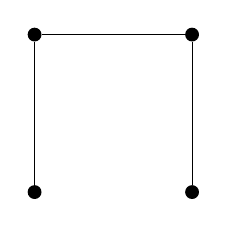
\begin{tikzpicture}[baseline={([yshift=-.5ex]current bounding box.center)}]
                \node[fill, circle, inner sep = 0, minimum size = 5pt] at (0, 0) (1) {};
                \node[fill, circle, inner sep = 0, minimum size = 5pt] at (2, 0) (2) {};
                \node[fill, circle, inner sep = 0, minimum size = 5pt] at (0, -2) (3) {};
                \node[fill, circle, inner sep = 0, minimum size = 5pt] at (2, -2) (4) {};
                \draw (1) -- (2);
                \draw (1) -- (3);
                \draw (2) -- (4);
            \end{tikzpicture}
        \end{gather*}
        Higher powers of a given coordinate would then, for example, give rise to diagrams with loops at a given vertex:
        \begin{gather*}
            A^{-1}_{11}A^{-1}_{12}A^{-1}_{22} =
            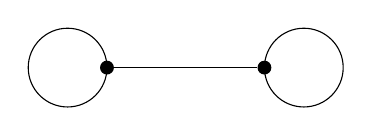
\begin{tikzpicture}[baseline={([yshift=-.5ex]current bounding box.center)}]
                \node[fill, circle, inner sep = 0, minimum size = 5pt] at (0, 0) (1) {};
                \node[fill, circle, inner sep = 0, minimum size = 5pt] at (2, 0) (2) {};
                \draw (-0.5, 0) circle (0.5);
                \draw (1) -- (2);
                \draw (2.5, 0) circle (0.5);
            \end{tikzpicture}
        \end{gather*}
    \end{example}

    \begin{remark}[Normalization]
        In practice, one often divides all Gaussian integrals by the quantity $I(A,0)$ to cancel the normalization factor. In the functional setting, this is even imperative since, as mentioned above, the normalization factor diverges for infinite-dimensional spaces.
    \end{remark}

\subsection{Generalizations}

    \newdef{Henstock--Kurzweil integral\footnotemark}{\index{integral!Henstock--Kurzweil}\index{integral!Perron}\index{integral!Denjoy}\index{integral!Luzin}\index{gauge|seealso{integral, Denjoy}}\index{integral!McShane}
    \footnotetext{Also called the \textbf{Perron}, \textbf{Lusin}, \textbf{(narrow) Denjoy} or \textbf{gauge} integral.}
        Consider the usual definition of the (proper) Riemann integral, where tagged partitions $P$ of $[a,b]$ are chosen and the integral is obtained as the limit of the Riemann sums
        \begin{gather}
            I = \sum_Pf(x_i)(t_i-t_{i-1})
        \end{gather}
        as the mesh size of the partitions goes to zero.

        Now, to obtain the generalized integral, consider a strictly positive function $\delta:[a,b]\mathbb{R}^{>0}$, the \textbf{gauge function}. Given such a gauge, a tagged partition $P$ is said to be \textbf{$\delta$-fine} if
        \begin{gather}
            [t_{i-1},t_i]\subset[x_i-\delta(x_i),x_i+\delta(x_i)]
        \end{gather}
        for subintervals in the partition.\footnote{If the condition $x_i\in[t_{i-1},t_i]$ in the definition of tagged partitions is dropped, the \textbf{McShane integral} is obtained. This can be shown to be equivalent to the \textit{Lebesgue integral} (see \cref{chapter:measure}).}

        If the integral exists, it is given by the number $I\in\mathbb{R}$ such that for all $\varepsilon>0$ there exists a gauge $\delta:[a,b]\rightarrow\mathbb{R}^{>0}$ such that, if $P$ is $\delta$-fine, then
        \begin{gather}
            \left\vert I-\sum_Pf(x_i)(t_i-t_{i-1})\right\vert<\varepsilon\,.
        \end{gather}
    }
    \begin{remark}[Riemann integral]\index{integral!Riemann}
        If the gauge functions are chosen to be constant, the classical $(\varepsilon,\delta)$-definition of ordinary Riemann integrals is obtained.
    \end{remark}

    The following statement can be seen as a refinement of \cref{topology:heine_borel}. Moreover, it is also sometimes known as the \textbf{Borel--Lebesgue theorem}.\index{Borel--Lebesgue}
    \begin{property}[Cousin]\index{Cousin}
        For every gauge $\delta:[a,b]\rightarrow\mathbb{R}^{>0}$, there exists a $\delta$-fine partition. 
    \end{property}

    \begin{property}[Integrability]
        If $f:[a,b]\rightarrow\mathbb{R}$ is bounded, then the following are equivalent:
        \begin{itemize}
            \item $f$ is Henstock--Kurzweil integrable, and
            \item $f$ is \textit{Lebesgue integrable} (see \cref{chapter:measure}).
        \end{itemize}
        More generally, a function $f:[a,b]\rightarrow\mathbb{R}$ is Henstock--Kurzweil integrable if and only if both $f$ and $|f|$ are \textit{Lebesgue integrable}.
    \end{property}

    The following property shows that `improper' Henstock--Kurzweil integrals are only truly improper for unbounded domains.
    \begin{property}[Hake]\index{Hake}
        \begin{gather}
            \Int_a^bf\,dx = \lim_{c\nearrow b}\Int_a^cf\,dx\,,
        \end{gather}
        whenever either side exists.
    \end{property}

    One of the most important arguments for using the Henstock--Kurzweil integral is its refinement of the Second Fundamental Theorem of Calculus~\ref{calculus:second_fundamental_theorem}. Note that the theorem for the Riemann integral required that the derivative was integrable. The gauge integral relaxes this condition.
    \begin{theorem}[Second fundamental theorem of calculus]
        Let $f:[a,b]\rightarrow\mathbb{R}$ be differentiable, then
        \begin{gather}
            \Int_a^xf'(x')\,dx' = f(x)-f(a)\text{\ \ a.e.}
        \end{gather}
    \end{theorem}

\section{Convexity}

    \newdef{Convex set}{\index{convex}\index{hull}\label{calculus:convex}
        A subset of $X$ of a vector space $V$ (\cref{linalgebra:vector_space}) is said to be convex if $x,y\in X$ implies that $\bigl\{\lambda x+(1-\lambda)y\mid\lambda\in[0,1]\bigr\}\subset X$, i.e.~if all straight lines connecting elements of the set are completely contained in that set. The \textbf{convex hull} of a subset $X$ is defined as the smallest convex subset containing $X$.
    }

    \newdef{Extreme point}{\index{extreme!point}\label{calculus:extreme_point}
        Consider a convex set $X$. The extreme points of $X$ are the points $p\in X$ such that, if
        \begin{gather}
            p = \lambda p_1 + (1-\lambda)p_2
        \end{gather}
        for some $p_1,p_2\in X$ and $\lambda\in[0,1]$, then $p_1=p_2=p$.
    }

    \newdef{Convex function}{\label{calculus:convex_function}
        Let $X$ be a convex set. A function $f:X\rightarrow\mathbb{R}$ is said to be convex if for all $x,y\in X$ and $\lambda\in[0,1]$:
        \begin{gather}
            f\bigl(\lambda x + (1-\lambda)y\bigr)\leq t\lambda(x) + (1-\lambda)f(y)\,.
        \end{gather}
        For the definition of a \textbf{concave} function, the inequality has to be turned around.
    }
    \newdef{Linear map}{\index{linear!map}
        A function $f:X\rightarrow\mathbb{R}$ is linear if and only if it is both convex and concave.
    }

    \begin{theorem}[Karamata's inequality]\index{Karamata}
        Consider an interval $I\subset\mathbb{R}$ and let $f:I\rightarrow\mathbb{R}$ be a convex function. If $(x_1,\ldots,x_n)$ is a tuple that majorizes $(y_1,\ldots,y_n)$, i.e.
        \begin{gather}
            \sum_{i=1}^nx_i = \sum_{i=1}^ny_i
        \end{gather}
        and
        \begin{gather}
            x_{(1)} + \cdots + x_{(k)}\geq y_{(1)} + \cdots + y_{(k)}
        \end{gather}
        for all $k\leq n$, where $x_{(i)}$ denotes the $i^{\text{th}}$ largest element of $(x_1,\ldots,x_n)$, then
        \begin{gather}
            \sum_{i=1}^nf(x_i)\geq\sum_{i=1}^nf(y_i)\,.
        \end{gather}
    \end{theorem}

    The following inequality can be derived directly from the definition of convexity by induction.
    \begin{theorem}[Jensen's inequality]\index{Jensen's inequality}\label{calculus:jensen_inequality}
        Let $f$ be a convex function and consider a point $\{a_i\}_{i\leq n}$ in the probability simplex $\Delta^n$ (\cref{topology:standard_simplex}).
        \begin{gather}
            f\left(\sum_{i=1}^na_ix_i\right)\leq\sum_{i=1}^na_if(x_i)\,.
        \end{gather}
    \end{theorem}

    \newdef{Legendre transformation}{\index{Legendre!transformation}\label{calculus:legendre}
        Consider a function $f:\mathbb{R}\rightarrow\mathbb{R}$. In certain cases (especially in physics) it is sometimes useful to replace the argument $x$ by the slope of $f$ at $x$, i.e.~to perform the transformation
        \begin{gather}
            x\longrightarrow f'(x)\,.
        \end{gather}
        However, it should be clear that this transformation is not always well-defined and, even if it is, it does not always preserve all the information contained in $f$.

        These conditions are satisfied exactly if $f$ is convex (or concave). In this case, the Legendre transform of $f$ is defined as
        \begin{gather}
            f^*(x^*) := \sup_x\bigl(x^*x - f(x)\bigr)\,.
        \end{gather}
        Now, consider the case where $f$ is differentiable. The above supremum can then be obtained by differentiating the right-hand side and equating it to zero. This results in $x^* = f'(x)$, which is exactly the transformation that was required. By expressing everything in terms of the Legendre tranformed quantity $x^*$, one can also find the derivative of $f^*$:
        \begin{gather}
            \deriv{f^*}{x^*}(x^*) = x(x^*)\,.
        \end{gather}
    }

    \begin{property}[Alternative characterization]\label{calculus:legendre_condition}
        In fact, up to an additive constant, the condition
        \begin{gather}
            (f^*)' = (f')^{-1}
        \end{gather}
        uniquely determines the Legendre transformation.
    \end{property}
    \begin{remark}
        These definitions can easily be extended to higher dimensions ($n\geq2$).
    \end{remark}

\section{Trigonometry}

    \newdef{Trigonometric functions}{\index{sine}\index{cosine}\index{tangent}
        Consider \cref{fig:right_triangle}. In a right(-angled) triangle, the trigonometric functions of the angle $\theta$ are defined as follows:
        \begin{gather}
                \sin(\theta) := \frac{y}{x}\qquad\qquad
                \cos{\theta} := \frac{z}{x}\qquad\qquad
                \tan(\theta) := \frac{y}{z}
        \end{gather}
    }
    \begin{result}
        \begin{gather}
            \tan(\theta) = \frac{\sin(\theta)}{\cos(\theta)}
        \end{gather}
    \end{result}

    \begin{figure}[ht!]
        \centering
        \begin{tikzpicture}
            \draw (0, 0) node[below left]{$A$} -- node[left]{$z$} (0, 2) node[above left]{$B$} node[below = .5cm, right = .1cm]{$\theta$} -- node[above right]{$x$} (5, 0) node[below right]{$C$} -- node[below]{$y$} (0, 0);
        \end{tikzpicture}
        \caption{Right(-angled) triangle.}
        \label{fig:right_triangle}
    \end{figure}
\chapter{Complex calculus}
\section{Complex algebra}
	
	The set of complex numbers $\mathbb{C}$ forms a 2-dimensional vector space over the field of real numbers. Furthermore the operations of complex addition and complex multiplication also turn the complex numbers into a field.

	\newdef{Complex conjugate}{\index{complex conjugate}
    		The complex conjugate $\overline{z}:a+bi\mapsto a-bi$ is an involution, i.e. $\overset{=}{z} = z$. It is sometimes denoted by $z^*$ instead of $\overline{z}$.
	}
    
	\newformula{Real/imaginary part}{
    		A complex number $z$ can also be written as $\operatorname{Re}(z) + i\operatorname{Im}(z)$ where
        	\begin{equation}
			\operatorname{Re}(z) = \stylefrac{z+\overline{z}}{2}
		\end{equation}
        	\begin{equation}
			\operatorname{Im}(z) = \stylefrac{z - \overline{z}}{2i}
		\end{equation}
	}
	
	\newdef{Riemann sphere}{\index{Riemann!sphere}
		Consider the one-point compactification\footnote{See definition \ref{topology:alexandrov_compactification}.} $\overline{\mathbb{C}} = \mathbb{C}\cup\{\infty\}$. This set is called the Riemann sphere or extended complex plane. The standard operations on $\mathbb{C}$ can be generalized to $\overline{\mathbb{C}}$ in the following way:
		\begin{align}
			z + \infty &= \infty\nonumber\\
			z * \infty &= \infty\\
			\frac{z}{\infty} &= 0\nonumber
		\end{align}
		for all non-zero $z \neq \infty$. As there exists no multiplicative inverse for $\infty$ the Riemann sphere does not form a field.
	}

\section{Holomorphic functions}
        
        \begin{definition}[Holomorphic]\index{holomorphic}
            A function $f$ is holomorphic on an open set $U$ if it is complex differentiable at every point $z_0\in U$. 
        \end{definition}
        
        \begin{theorem}[Cauchy-Riemann conditions]\index{Cauchy!Cauchy-Riemann conditions}
            A function $f(z)$ with real-differentiable real and imaginary parts is holomorphic if and only if it satisfies the following conditions:
            \begin{equation}
                \label{complexcalculus:cauchy_riemann}
                \boxed{\pderiv{u}{x} = \pderiv{v}{y} \text{\qquad and\qquad} \pderiv{u}{y} = -\pderiv{v}{x}}
            \end{equation}
            or equivalently:
            \begin{equation}
                \label{complexcalculus:holomorphic_alternative_condition}
                \boxed{\pderiv{f}{\overline{z}} = 0}
            \end{equation}
        \end{theorem}
        \remark{The condition $f(z)\in C^1(\Omega)$ was made redundant by the Cauchy-Goursat theorem.}

	\begin{property}
		Functions $u,v$ satisfying the CR-conditions are harmonic functions, i.e. they satisfy Laplace's equation.
	\end{property}
    \begin{property}
		Functions $u,v$ satisfying the CR-conditions have orthogonal level curves \ref{set:level_set}.
	\end{property}

\section{Complex integrals}
		In this and further sections, all contours have been chosen to be evaluated counterclockwise (by convention). To obtain results concerning clockwise evaluation, most of the time adding a minus sign is sufficient.
        
        \newdef{Contour}{\index{contour}
        	A contour is a curve $z(t)$ that can be parametrized by
            \begin{equation}
            	\left.
				\begin{array}{c}
                	x = x(t)\\
                    y = y(t)
                \end{array}\right\}
                \rightarrow z(t) = z = x+iy
			\end{equation}
        }
        \newformula{Complex contour integral}{
        	The complex contour integral of a function $f(z) = u(z) + iv(z)$ is defined as the following line integral:
        	\begin{equation}
            	\label{complexcalculus:contour_integral}
				\int_{z_1}^{z_2}f(z)dz = \int_{(x_1,y_1)}^{(x_2,y_2)}[u(x,y) + iv(x,y)](dx + idy)
			\end{equation}
        }
        
        \begin{theorem}[Cauchy's Integral Theorem]\index{Cauchy!integral theorem}
        	Let $\Omega$ be a simply-connected subset of $\mathbb{C}$ and let $f$ be a holomorphic function on $\Omega$. Then for every closed rectifiable contour $C$  in $\Omega$:
            \begin{equation}
				\label{complexcalculus:cauchy_integral_theorem}
                \boxed{\oint_C f(z) dz = 0}
			\end{equation}
        \end{theorem}
        \result{The contour integral of a holomorphic function depends only on the limits of integration and not on the contour connecting them.}
        
        \begin{formula}[Cauchy's Integral Formula]\index{Cauchy!integral formula}
        	Let $\Omega$ be a connected subset of $\mathbb{C}$ and let $f$ be a holomorphic function on $\Omega$. Let $C$ be a contour in $\Omega$. For every point $z_0$ inside $C$ we find:
            \begin{equation}
				\label{complexcalculus:cauchy_integral_formula}
                \boxed{f(z_0) = \frac{1}{2\pi i}\oint_C \frac{f(z)}{z - z_0} dz}
			\end{equation}
        \end{formula}

        \begin{result}[Analytic function]\index{analytic}
			Let $\Omega$ be a connected subset of $\mathbb{C}$ and $C$ a closed contour in $\Omega$. If $f$ is holomorphic on $\Omega$ then $f$ is analytic\footnotemark\ on $\Omega$ and:
            \begin{equation}
				\label{complexcalculus:cauchy_integral_formula_derivative}
                \boxed{f^{(n)}(z_0) = \frac{1}{2\pi i}\oint_C f(z) \frac{n!}{(z - z_0)^{n+1}} dz}
			\end{equation}
            Furthermore, the derivatives are also holomorphic on $\Omega$.
		\end{result}
        \footnotetext{See definition \ref{calculus:analytic}.}
        
        \begin{theorem}[Morera's Theorem]\index{Morera's theorem}
            If $f$ is continuous on a connected open set $\Omega$ and $\oint_C f(z) dz = 0$ for every closed contour $C$ in $\Omega$, then $f$ is holomorphic on $\Omega$.
		\end{theorem}
        
        \begin{definition}[Meromorphic]\index{meromorphic}
			A function $f$ is called meromorphic when it is analytic on the whole complex plane with exception of isolated singularities. 
		\end{definition}
        
\section{Laurent series}
    	\begin{definition}[Laurent series]\index{Laurent!series}
        	\label{complexcalculus:laurent_series}
            If $f$ is function, analytic on an annulus A, then $f$ can be expanded as the following series:
            \begin{equation}
                f(z) = \sum^{\infty}_{n=-\infty} a_n (z - z_0)^n \qquad \text{with} \qquad a_n = \frac{1}{2\pi i} \oint \frac{f(z')}{(z' - z_0)^{n+1}} dz'
			\end{equation}
		\end{definition}
        
        \begin{remark}
			The Laurent series of an analytic function $f$ converges uniformly to $f$ in the ring shaped region ('\textit{annulus}') $R_1 < |z - z_0| < R_2$, with $R_1$ and $R_2$ the distances from $z_0$ to the two closest poles.
        \end{remark}
        
        \newdef{Principal part}{\index{principal part}
        	The principal part of a Laurent series is defined as the sum:
            \[
            	\sum_{n=-\infty}^{-1}a_n(z-z_0)^n
            \]
        }
        
\section{Analytic continuation}
	\begin{theorem}[Schwarz' reflection principle]\index{Schwarz!reflection principle}
		Let $f(z)$ be analytic on the upper half plane. If $f(z)$ is real when $z$ is real then
        \begin{equation}
        	f(\overline{z}) = \overline{f(z)}
        \end{equation}
	\end{theorem}
    
\section{Singularities}
\subsection{Poles}
	\newdef{Pole}{\index{pole}
    	A function $f(z)$ has a pole of order $m>0$ at a point $z_0$ if its Laurent series at $z_0$ satisfies $\forall n<-m:a_n = 0$ and $a_{-m}\neq0$.
    }
    
    \newdef{Essential singularity}{\index{essential singularity}
    	A function $f(z)$ has an essential singularity at a point $z_0$ if its Laurent series at $z_0$ satisfies $\forall n\in\mathbb{N}:a_{-n}\neq0$, i.e. its Laurent series has infinitely many negative degree terms.
    }
    
    \begin{theorem}[Picard's great theorem]\index{Picard!great theorem}
		Let $f(z)$ be an analytic function with an essential singularity at $z_0$. On every punctured neighbourhood of $z_0$, $f(z)$ takes on all possible complex values, with at most a single exception, infinitely many times.
	\end{theorem}
    
    \newmethod{Frobenius transformation}{\index{Frobenius!transformation}
    	To study the behaviour of a function $f(z)$ at $z\rightarrow\infty$, one should apply the Frobenius transformation $h = 1/z$ and study the limit $\lim_{h\rightarrow0}f(h)$.
    }

\subsection{Branch cuts}
	
	\newdef{Branch point}{
    		Let $f(z)$ be a complex valued function. A point $z_0$ such that there exists no neighbourhood $|z-z_0|<\varepsilon$ where $f(z)$ is single valued is called a branch point.
	}
	\newdef{Branch cut}{
    		A line connecting exactly two branch points is called a branch cut. One of the branch points can be at infinity. In case of multiple branch cuts, they do not cross. 
	}
	
	\newformula{Roots}{
    		Let $z\in\mathbb{C}$. The $n^{th}$ roots\footnotemark\ of $z$ are given by:
        	\begin{equation}
			z^{1/n} = \sqrt[n]{|z|}e^{i\frac{\operatorname{arg}(w) + 2\pi k}{n}}
		\end{equation}
        	where $k\in\{0,1,...,n\}$.
		\footnotetext{Also see theorem \ref{linalgebra:fundamental_theorem_of_algebra}.}
	}
	\newformula{Complex logarithm}{\index{logarithm}
    		\begin{equation}
			\operatorname{LN}(z) = \ln(r) + i(\theta + 2\pi k)
		\end{equation}
	}
	From these two formulas it is clear that the complex roots and logarithms are multi-valued functions. To get an unambiguous image it is necessary to fix a value of the parameter $k$. By doing this there will arise curves in the complex plane where the function is discontinuous. These are the branch cuts.
    
    \begin{example}
		Consider the complex function \[f(z) = \stylefrac{1}{\sqrt{(z-z_1)...(z-z_n)}}\] This function has singularities at $z_1,...,z_n$. Furthermore if $n$ is even, this function will have $n$ branch points with no branch points at infinity. This implies that the points can be grouped in pairs connected by non-intersecting branch cuts. If $n$ is odd, this function will have $n$ 'finite' branch points and one branch point at infinity. The 'finite' branch points will be grouped in pairs connected by non-intersecting branch cuts and the remaining branch point will be joined to infinity by a branch cut which does not intersect the others.(See \cite{branchcut} for the proof.)
	\end{example}
    
\subsection{Residue theorem}
	
	\newdef{Residue}{
    		By applying formula \ref{complexcalculus:contour_integral} to a polynomial function we find:
    		\begin{equation}
    			\int_C(z-z_0)^ndz = 2\pi i\delta_{n,-1}
    		\end{equation}
    		where $C$ is a circular contour around the pole $z = z_0$. This means that integrating a Laurent series around a pole isolates the coefficient $a_{-1}$. This coefficient is therefore called the residue of the function at the given pole.
	}
	\begin{notation}
		The residue of a complex function $f(z)$ at a pole $z_0$ is denoted by $\text{Res}[f(z)]_{z=z_0}$.
	\end{notation}
	
	\begin{formula}
    		For a pole of order $m$, the residue is calculated as follows:
		\begin{equation}
			\label{complexcalculus:residue}
            		\operatorname{Res}\left[f(z)\right]_{z=z_j} = a_{-1} = \lim_{z\rightarrow z_0} \stylefrac{1}{(m - 1)!} \left(\pderiv{}{z}\right)^{m-1}\left(f(z)(z-z_0)\right)
		\end{equation}
	        For essential singularities the residue can be found by writing out the Laurent series explicitly.
	\end{formula}

	\begin{theorem}[Residue theorem]\index{Residue theorem}
        	\label{complexcalculus:residue_theorem}
            If $f(z)$ is a meromorphic function in $\Omega$ and if $C$ is a closed contour in $\Omega$ which contains the poles $z_j$ of $f(z)$, then:
            \begin{equation}
                \boxed{\oint_Cf(z)dz = 2\pi i\sum_j \operatorname{Res}\left[f(z)\right]_{z=z_j}}
			\end{equation}
	\end{theorem}
    \remark{For poles on the contour $C$, only half of the residue contributrs to the integral.}

\section{Limit theorems}
    	\begin{theorem}[Small limit theorem]\index{Limit theorem}
			\label{complexcalculus:theorem:small_limit}
            Let $f$ be a function that is holomorphic almost every where on $\mathbb{C}$. Let the contour $C$ be a circular segment with radius $\varepsilon$ and central angle $\alpha$.
            If $z$ is parametrized as $z = \varepsilon e^{i\theta}$ then\[\int_Cf(z)dz = i\alpha A\]
            with \[A = \lim_{\varepsilon\rightarrow0}f(z)\]
		\end{theorem}
        \begin{theorem}[Great limit theorem]
			\label{complexcalculus:theorem:great_limit}
            Let $f$ be a function that is holomorphic almost every where on $\mathbb{C}$. Let the contour $C$ be a circular segment with radius $R$ and central angle $\alpha$.
            If $z$ is parametrized as $z = Re^{i\theta}$ then\[\int_Cf(z)dz = i\alpha B\]
            with \[B = \lim_{R\rightarrow+\infty}f(z)\]
		\end{theorem}
        \begin{theorem}[Jordan's lemma]\index{Jordan}
			\label{complexcalculus:theorem:jordan}
            Let $g$ be a continuous function with $g(z) = f(z)e^{bz}$. Let the contour $C$ be a semicircle lying in the half-plane bounded by the real axis and oriented away of the point $\overline{b}i$. If $z$ is parametrized as $z=Re^{i\theta}$ and \[\lim_{R\rightarrow\infty}f(z) = 0\] then\[\int_Cg(z)dz = 0\]
		\end{theorem}

\chapter{Measure Theory and Lebesgue Integration}
\label{chapter:lebesgue}

\section{Measure}
\subsection{General definitions}

	\newdef{Measure}{\index{measure}\index{$\sigma$-additivity}
    	\label{lebesgue:measure}
		Let $X$ be a set. Let $\Sigma$ be a $\sigma$-algebra over $X$. A function $\mu:\Sigma\rightarrow\overline{\mathbb{R}}$ is called a measure if it satisfies the following conditions:
		\begin{enumerate}
			\item Non-negativity: $\forall E\in\Sigma:\mu(E) \geq0$
            \item Null empty set: $\mu(\emptyset) = 0$
            \item Countable-additivity\footnotemark\ : $\forall i\neq j:E_i\cap E_j=\emptyset\implies\mu\left(\bigcup_{i=1}^\infty E_i\right) = \sum_{i=1}^\infty \mu(E_i)$
		\end{enumerate} 
    }
    \footnotetext{also called $\sigma$-additivity}
    
    \newdef{Measure space}{
    	\label{lebesgue:measure_space}
    	The pair $(X, \Sigma)$ is called a measurable space. The elements $E\in\Sigma$ are called measurable sets. The triplet $(X, \Sigma, \mu)$ is called a measure space.
    }
    
	\newdef{Almost everywhere\footnotemark}{
		\footnotetext{In probability theory this is foten often called \textbf{almost surely}.}
		Let $(X, \Sigma, \mu)$ be a measure space. A property $P$ is said to hold on X almost everywhere (a.e.) if it satisfies the following equation:
	        \begin{equation}
		        \label{lebesgue:almost_everywhere}
        		\mu\left(\{x\in X:\neg P(x)\}\right) = 0
        	\end{equation}
	}
    
    \newdef{Complete measure space}{
    	The measure space $(X,\Sigma,\mu)$ is said to be complete if for every $E\in\Sigma$ with $\mu(E) = 0$ the following property holds for all $A\subset E$:
        \[
        	A\in\Sigma \quad\text{and}\quad \mu(A) = 0
		\]
    }
    \newdef{Completion}{
    	Let $\mathcal{F},\mathcal{G}$ be $\sigma$-algebras over a set $X$. $\mathcal{G}$ is said to be the completion of $\mathcal{F}$ if it is the smallest $\sigma$-algebra such that the measure space $(X,\mathcal{G},\mu)$ is complete.
    }
    
    \newdef{Regular Borel measure}{
    	Let $\mu$ be a non-negative countably additive set function defined on $\mathcal{B}$. $\mu$ is called a regular Borel measure if it satisifes following equations for every Borel set $B$:
    	\begin{equation}
			\label{lebesgue:regular_borel_measure}
            \begin{array}{ccl}
				\mu(B)& =& \inf\{\mu(O):O \text{ open}, O\supset B\}\\
                \mu(B)& =& \sup\{\mu(F):F \text{ closed}, F\subset B\}
			\end{array}
		\end{equation}
    }

	\newdef{\texorpdfstring{$\sigma$-}\ finite measure}{\index{$\sigma$-finite}
    	\label{lebesgue:sigma_finite_measure}
    	Let $(\Omega,\mathcal{F},P)$ be a measure space. The measure $P$ is said to be $\sigma$-finite if there exists a sequence $(A_i)_{i\in\mathbb{N}}$ of measurable sets such that $\bigcup_{i=1}^{+\infty}A_i = \Omega$ with $\forall A_i:P(A_i) < +\infty$.
    }
    
    \begin{method}
    	To show that two measures coincide on a $\sigma$-algebra, it suffices to show that they coincide on the generating sets and apply the monotone class theorem \ref{set:theorem:monotone_class}.
    \end{method}


	\subsection{Lebesgue measure}
    	\newformula{Length of an interval}{\index{length}
        	The length of an open interval $I=(a,b)$ is defined as:
            \begin{equation}
				\label{lebesgue:interval_length}
                l\left(I\right) = b-a
			\end{equation}
        }
        
        \newdef{Null set}{\index{null set}
        	A set $A\subset\mathbb{R}$ is called a null set if it can be covered by a sequence of intervals of arbitrarily small length: $\forall\varepsilon>0$ there exists a sequence $(I_n)_{n\in\mathbb{N}}$ such that
            \begin{equation}
				A \subseteq \bigcup_{n=1}^{+\infty}I_n
			\end{equation}
            with
            \begin{equation}
				\sum_{i=1}^{+\infty}l(I_n) < \varepsilon
			\end{equation}
        }
        \begin{theorem}
			Let $(E_i)_{i\in\mathbb{N}}$ be a sequence of null sets. The union $\bigcup_{i=1}^{+\infty}E_i$ is also null.
		\end{theorem}
        \result{
        	\label{lebesgue:theorem:countable_set_is_null}
            Any countable set is null.
		}
    
    	\newdef{Outer measure}{\index{outer measure}
        	Let $X\subseteq\mathbb{R}$ be an open set. The (Lebesgue) outer measure is defined as:
            \begin{equation}
				\label{lebesgue:outer_measure}
                \boxed{m^*(X) = \inf\left\{\sum_{i=1}^{+\infty} l(I_i)\text{ with }(I_i)_{i\in\mathbb{N}} \text{ a sequence of open intervals that covers }X\right\}}
			\end{equation}
        }
        
        \begin{property}
			Let $I$ be an interval. The outer measure equals the length: $m^*(I) = l(I)$.
		\end{property}
        \begin{property}
			The outer measure is translation invariant: $m^*(A + t) = m^*(A)\quad,\forall A,t$
		\end{property}
        \begin{property}
			$m^*(A) = 0$ if and only if $A$ is null.
		\end{property}
        \begin{property}
			If $A\subset B$ then $m^*(A)\leq m^*(B)$.
		\end{property}
        \begin{property}[Countable subadditivity]
        	For every sequence of sets $(E_i)_{i\in\mathbb{N}}$ the following inequality holds: 
			\begin{equation}
				m^*\left(\bigcup_{i=1}^{+\infty}E_i\right) \leq \sum_{i=1}^{+\infty}m^*(E_i)
			\end{equation}
		\end{property}
        
        \begin{theorem}[Carath\'eodory's criterion / Lebesgue measure]
        	\index{Carath\'eodory!criterion}\index{Lebesgue!measure}\index{measurable!set}
        	Let $X$ be a set. If $X$ satisfies the following equation, it is said to be Lebesgue measurable:
            \begin{equation}
				\label{lebesgue:lebesgue_measure}
                \forall E\subseteq\mathbb{R}:m^*(E) = m^*(E\cap X) + m^*(E\cap X^c)
			\end{equation}
            This is denoted by $X\in\mathcal{M}$ and the outer measure $m^*(X)$ is called the Lebesgue measure of $X$ denoted by $m(X)$.
        \end{theorem}
        \begin{property}
			All null sets and intervals are measurable.
		\end{property}
        \newprop{Countable additivity}{\index{countable!additivity}
        	For every sequence $(E_i)_{i\in\mathbb{N}}$ with $E_i\in\mathcal{M}$ satisfying $i\neq j:E_i\cap E_j = \emptyset$ the following equation holds:
        	\begin{equation}
				\boxed{m\left(\bigcup_{i=1}^{+\infty}E_i\right) = \sum_{i=1}^{+\infty}m(E_i)}
			\end{equation}
        }
        \sremark{Previous property, together with the properties of the outer measure, implies that the Lebesgue measure is indeed a proper measure as defined in \ref{lebesgue:measure}.}
        
        \begin{property}
			$\mathcal{M}$ is a $\sigma$-algebra\footnotemark\ over $\mathbb{R}$. 
		\end{property}
        \footnotetext{See definition \ref{set:sigma_algebra}.}
        
        \begin{theorem}
			For every $A\subset\mathbb{R}$ there exists a sequence $(O_i)_{i\in\mathbb{N}}$ of open sets such that:
            \begin{equation}
            	\label{lebesgue:theorem:open_cover_existence}
				A\subset\bigcap_iO_i\qquad\text{and}\qquad m\left(\bigcap_iO_i\right) = m^*(A)
			\end{equation}
		\end{theorem}
        \begin{theorem}
			For every $E\in\mathcal{M}$ there exists a sequence $(F_i)_{i\in\mathbb{N}}$ of closed sets such that:
            \begin{equation}
            	\label{lebesgue:theorem:closed_cover_existence}
				\bigcup_iF_i\subset E\qquad\text{and}\qquad m\left(\bigcup_iF_i\right) = m(E)
			\end{equation}
		\end{theorem}
        \sremark{The previous 2 theorems imply that the Lebesgue measure is a regular Borel measure \ref{lebesgue:regular_borel_measure}.}
        
        \begin{theorem}
			Let $E\subset\mathbb{R}$. $E\in\mathcal{M}$ if and only if for every $\varepsilon>0$ there exist an open set $O\supset E$ and a closed set $F\subset E$ such that $m^*(O\backslash E) < \varepsilon$ and $m^*(E\backslash F)<\varepsilon$.
		\end{theorem}
        
        \begin{property}
			Let $(A_i)_{i\in\mathbb{N}}$ be a sequence of sets with $\forall i:A_i\in\mathcal{M}$. The following two properties apply:
            \begin{equation}
            	\forall i: A_i\subseteq A_{i+1} \implies m\left(\bigcup_{i=1}^{+\infty}A_i\right) = \lim_{i\rightarrow+\infty}m(A_i)
			\end{equation}
            \begin{equation}
            	\forall i: A_i\supseteq A_{i+1} \land m(A_1)<+\infty\implies m\left(\bigcap_{i=1}^{+\infty}A_i\right) = \lim_{i\rightarrow+\infty}m(A_i)
			\end{equation}
		\end{property}
        \remark{This property is not only valid for the Lebesgue measure but for every countably additive set function.}
        \begin{property}
			The Lebesgue measure $m(X)$ is continuous at $\emptyset$, i.e. if $(A_i)_{i\in\mathbb{N}}\rightarrow\emptyset$ then $\displaystyle\lim_{i\rightarrow+\infty}m(A_i) = 0$.
		\end{property}
        
        \begin{theorem}
			$\mathcal{M}$ is the completion of $\mathcal{B}$.
		\end{theorem}
        \result{
        	\label{lebesgue:theorem:B_in_M}
        	$\mathcal{B}\subset\mathcal{M}\subset\mathcal{F}_{\mathbb{R}}$
		}
        
        \newdef{Restricted Lebesgue measure}{\index{Lebesgue!restricted measure}
        	Let $B\subset\mathbb{R}$ be a measurable set with measure $m(B)>0$. The restriction of the Lebesgue measure to the set $B$ is defined as follows:
            \begin{equation}
				\label{lebesgue:restricted_lebesgue_measure}
                \mathcal{M}_B = \left\{A\cap B:A\in\mathcal{M}\right\}\qquad\text{and}\qquad\forall E\in\mathcal{M}_B:m_B(E) = m(E)
			\end{equation}
            Furthermore, the measure space $(B,\mathcal{M}_B,m_B)$ is complete.
        }
        
    \subsection{Measurable functions}
    	\newdef{Measurable function}{\index{measurable!function}
        	\label{lebesgue:measurable_function}
        	A function $f$ is (Lebesgue) measurable if for every interval $I\subset\mathbb{R}:f^{-1}(I)\in\mathcal{M}$.
        }
        \newdef{Borel measurable function}{\index{Borel!measurable function}
        	\label{lebesgue:borel_measurable_function}
        	A function $f$ is called Borel measurable\footnotemark\ if for every interval $I\subset\mathbb{R}:f^{-1}(I)\in\mathcal{B}$.
        }
        \footnotetext{These functions are often simply called 'Borel functions'.}
        \remark{Inclusion \ref{lebesgue:theorem:B_in_M} implies that every Borel function is also Lebesgue measurable.}
        
        \begin{theorem}
			The class of Lebesgue measurable\footnotemark\ functions defined on $E\in\mathcal{M}$ is closed under multiplication and it forms a vector space.
		\end{theorem}
        \footnotetext{This property is also valid for Borel functions.}
        
        \begin{property}
			Following types of functions are measurable:
            \begin{itemize}
				\item monotone functions
                \item continuous functions
                \item indicator functions
			\end{itemize}
		\end{property}
		\begin{result}
			Let $f,g$ be measurable functions. Let $F:\mathbb{R}\times\mathbb{R}\rightarrow\mathbb{R}$ be a continuous function. The composition $F(f(x), g(x))$ is also measurable.
		\end{result}
        
        \begin{property}
			Let $f$ be a measurable function. The set\footnotemark\ $\{x:f(x) = a\}$ is also measurable for all $a\in\mathbb{R}$.
		\end{property}
        \footnotetext{This set is called the 'level set' of $f$.}

        \begin{theorem}
			Define following functions, which are measurable if $f$ is measurable as a result of previous properties:
            \begin{equation}
				\label{lebesgue:positive_part}
                f^+(x) = \left\{
                \begin{array}{ccc}
					f(x)&\text{if}&f(x)>0\\
                    0&\text{if}&f(x)\leq0
				\end{array}\right. = \max(f,0)
			\end{equation}
            \begin{equation}
				\label{lebesgue:negative_part}
                f^-(x) = \left\{
                \begin{array}{ccc}
					0&\text{if}&f(x)>0\\
                    -f(x)&\text{if}&f(x)\leq0
				\end{array}\right. = \max(-f,0)
			\end{equation}
            The function $f:E\rightarrow\mathbb{R}$ is measurable if and only if both $f^+$ and $f^-$ are measurable. Furthermore $f$ is measurable if $|f|$ is measurable, the converse is false.
		\end{theorem}

	\subsection{Limit operations}
    	\begin{property}
			Let $(f_i)_{i\in\mathbb{N}}$ be a sequence of measurable\footnotemark\ functions. The following operations are measurable:
            \begin{itemize}
				\item $\ds\min_{i\leq k}f_i$ and $\ds\max_{i\leq k}f_i$
                \item $\ds\inf_{i\in\mathbb{N}}f_i$ and $\ds\sup_{i\in\mathbb{N}}f_i$
                \item $\ds\liminf_{i\rightarrow+\infty}f_i$ and $\ds\limsup_{i\rightarrow+\infty}f_i$
			\end{itemize}
		\end{property}
        \footnotetext{This property is also valid for Borel functions.}
        \sremark{The measurability of the limit inferior and limit superior follows from their definitions and from the measurability of the $\inf/\sup$ and $\min/\max$.}
        
        \begin{property}
			Let $f$ be a measurable function. Let $g$ be a function such that $f=g$ almost everywhere. The function $g$ is measurable.
		\end{property}
        \result{A result of the previous two properties is the following: if a sequence of measurable functions converges pointwise a.e. then the limit is also a measurable function.}
	
        \newdef{Essential supremum}{\index{essential!supremum}
        	\begin{equation}
            	\label{lebesgue:essential_supremum}
                \esssup f = \sup\{z:f\geq z\text{ a.e.}\}
			\end{equation}
        }
        \newdef{Essential infimum}{\index{essential!infimum}
        	\begin{equation}
            	\label{lebesgue:essential_infimum}
                \essinf f = \inf\{z:f\leq z\text{ a.e.}\}
			\end{equation}
        }
        \begin{property}
			Let $f$ be a measurable function. $f\leq\esssup f\text{ a.e.}$ and $f\geq\essinf f\text{ a.e.}$ We also have that: $\esssup f\leq\sup f$ and $\essinf f\geq\inf f$, furthermore this last pair of inequalities becomes a pair of equalities if $f$ is continuous.
		\end{property}
        \begin{property}
			Let $f,g$ be measurable functions. $\esssup(f+g)\leq\esssup f + \esssup g$. An analogous inequality holds for the essential infimum.
		\end{property}

\section{Lebesgue integral}
\subsection{Simple functions}

    \newdef{Indicator function}{\index{indicator function}\label{lebesgue:indicator_function}
        \begin{gather}
    	    \mathbbm{1}_A(x) :=
            \begin{cases}
	            1&x\in A\\
                0&x\not\in A.
	        \end{cases}
	    \end{gather}
    }
    \newdef{Simple function}{\index{simple!function}\label{lebesgue:simple_function}
        A function $f:X\rightarrow\mathbb{R}$ on a measurable space $(X,\Sigma)$ that can be expressed as
        \begin{gather}
            f(x) = \sum_{i=1}^na_i\mathbbm{1}_{A_i}(x)
        \end{gather}
        for some $\{a_i\geq0\}_{i\leq n},\{A_i\}_{i\leq n}\subset\Sigma$ and $n\in\mathbb{N}$.
    }
    \begin{definition}[Step function]\index{step function}\label{lebesgue:step_function}
        If $(X,\Sigma)=(\mathbb{R},\mathcal{M})$ and the sets $A_i$ are intervals, the above function is often called a step function.
    \end{definition}

    \newdef{Lebesgue integral of simple functions}{\index{Lebesgue!integral}\label{lebesgue:integral_simple_function}
        Consider a simple function $\varphi$ on a measure space $(X,\Sigma,\mu)$. The Lebesgue integral of $\varphi$ over a measurable set $A\in\Sigma$ with respect to $\mu$ is given by
        \begin{gather}
            \int_A\varphi\,d\mu := \sum_{i=1}^na_i\mu(A\cap A_i).
        \end{gather}
        As usual, if the domain of integration is not mentioned explicitly, an integral over the whole space $X$ is implied.
    }
    \begin{example}
        Let $\mathbbm{1}_\mathbb{Q}$ be the indicator function of the rational numbers. Contrary to the case of Riemann integrals, the above definition makes it possible to integrate the rational indicator function over the real line:
        \begin{gather}
            \int_\mathbb{R}\mathbbm{1}_\mathbb{Q}\,d\lambda = 1\times\lambda(\mathbb{Q}) + 0\times\lambda(\mathbb{R}\backslash\mathbb{Q}) = 0,
        \end{gather}
        where the measure of the rational numbers is 0 because it is a countable set (Corollary \ref{lebesgue:countable_set_is_null}).
    \end{example}

\subsection{Measurable functions}

    \newdef{Integral for nonnegative functions}{\index{Lebesgue!integral}\label{lebesgue:integral}
        The definition for simple functions can be generalized to nonnegative measurable functions $f$ as follows:
        \begin{gather}
            \int_Af\,d\mu := \sup\left\{\int_A\varphi\,d\mu\,\middle\vert\,\varphi\text{ a simple function such that }\varphi\leq f\right\}.
        \end{gather}
        This integral is always nonnegative.
    }

    \begin{formula}
        The following equality allows to change the domain of integrals:
        \begin{gather}
            \label{lebesgue:domain_change}
            \int_Af\,d\mu = \int_Xf\mathbbm{1}_A\,d\mu.
        \end{gather}
    \end{formula}

    \begin{property}
        The Lebesgue integral over a null set is 0.
    \end{property}

    \begin{theorem}[Mean value theorem]\index{mean!value theorem}
        If $a\leq f(x)\leq b$, then $a\lambda(A)\leq\int_Af\,d\lambda\leq b\lambda(A)$.
    \end{theorem}

    \begin{property}
        Let $f$ be a nonnegative measurable function. There exists an increasing sequence $\seq{\varphi}$ of simple functions such that $\varphi_n\nearrow f$. Moreover, if $f$ is bounded on $A\in\Sigma$, the sequence can be chosen to be uniformly convergent on $A$.
    \end{property}

\subsection{Integrable functions}

    \newdef{Integrable function}{\index{integrable}\label{lebesgue:integrable_function}
        Let $A$ be a measurable subset of a measure space $(X,\Sigma,\mu)$. A measurable function $f$ is said to be integrable over $A$ if both $\int_Af^+\,d\mu$ and $\int_Af^-\,d\mu$ are finite. The Lebesgue integral of $f$ over $A$ is then defined as
        \begin{gather}
            \int_Af\,d\mu := \int_Af^+\,d\mu - \int_Af^-\,d\mu.
        \end{gather}
        If only one of the functions $f^+,f^-$ is finite, $f$ is said to be \textbf{quasi-integrable}.
    }

    \begin{property}[Absolute integrability]\label{lebesgue:absolute_integrability}
        $f$ is integrable if and only if $|f|$ is integrable. Furthermore, $\int_A|f|\,d\mu = \int_Af^+\,d\mu + \int_Af^-\,d\mu$.
    \end{property}
    \begin{property}
        Let $f,g$ be integrable functions on a measure space $(X,\Sigma,\mu)$. The following important properties hold:
        \begin{itemize}
            \item\textbf{Linearity}: $\int_A(f+\lambda g)d\mu = \int_Af\,d\mu/\lambda\int_Ag\,d\mu$ for all $\lambda\in\mathbb{R}$
            \item\textbf{Monotonicity}: $f\leq g$ a.e. implies $\int_Af\,d\mu\leq\int_Ag\,d\mu$ and $\forall A\in\Sigma:\int_Af\,d\mu\leq\int_Ag\,d\mu\implies f\leq g$ a.e.
            \item\textbf{Finiteness}: $f$ is finite a.e.
            \item $|\int_Af\,d\mu|\leq\int_A|f|\,d\mu$.
            \item $\int_Af\,d\mu=0,\forall A\in\Sigma\implies f=0$ a.e.
        \end{itemize}
    \end{property}

    \begin{definition}[Lebesgue integrable functions]
        The set of integrable functions over a set $A\in\mathcal{M}$ forms the vector space $\mathcal{L}^1(A)$.
    \end{definition}

    \begin{property}
        Let $f\in\mathcal{L}^1$ and $\varepsilon>0$. There exists a continuous (or step or even simple) function $g$, vanishing outside a finite (or even compact) set, such that $\int|f-g|\,d\mu<\varepsilon$.
    \end{property}

    \newdef{Locally integrable function}{\index{locally!integrable}\label{lebesgue:locally_integrable}
        A measurable function is said to be locally integrable if it is integrable on every compact subset of its domain. The space of locally integrable functions is denoted by $\mathcal{L}^1_{\mathrm{loc}}$.
    }
    \begin{example}
        All continuous functions are locally integrable.
    \end{example}

    \begin{property}[Absolute continuity]\index{continuity!absolute}\label{lebesgue:measure_by_integral}
        Let $f\geq0$ be a measurable function. The mapping $A\mapsto\int_Af\,d\mu$ defines a measure that is $\sigma$-finite if $f$ is locally integrable and finite if $f$ is integrable. Furthermore, this measure is said to be absolutely continuous (with respect to $\mu$). See Section \ref{section:Radon-Nikodym} for a generalization to arbitrary measures.
    \end{property}

\subsection{Convergence theorems}

    \begin{theorem}[Fatou's lemma]\index{Fatou}\label{lebesgue:fatous_lemma}
        Let $\seq{f}$ be a sequence of nonnegative measurable functions.
        \begin{gather}
            \int_A\left(\liminf_{n\rightarrow\infty}f_n\right)\,d\mu \leq \liminf_{n\rightarrow\infty}\int_Af_n\,d\mu
        \end{gather}
    \end{theorem}
    \begin{theorem}[Monotone convergence]\index{monotone!convergence theorem}\label{lebesgue:monotone_convergence_theorem}
        Let $A$ be measurable and let $\seq{f}$ be an increasing sequence of nonnegative measurable functions such that $f_n\nearrow f$ pointwise a.e.
        \begin{gather}
            \int_Af\,d\mu = \lim_{n\rightarrow\infty}\int_Af_n\,d\mu.
        \end{gather}
    \end{theorem}

    \begin{method}\label{lebesgue:linear_proofs}
        To prove results concerning integrable functions in spaces such as $\mathcal{L}^1$ it is often useful to proceed as follows:
        \begin{enumerate}
            \item Verify that the property holds for indicator functions. (This often follows by definition.)
            \item Use linearity to extend the property to simple functions.
            \item Apply the monotone convergence theorem to show that the property holds for all nonnegative measurable functions.
            \item Extend the property to all integrable functions by decomposing $f = f^+-f^-$ and applying linearity again.
        \end{enumerate}
    \end{method}

    \begin{theorem}[Dominated convergence]\index{dominated convergence theorem}\label{lebesgue:dominated_convergence_theorem}
        Let $A$ be measurable set and consider a sequence of measurable functions $\seq{f}$ such that $\forall n\in\mathbb{N}:|f_n|\leq g$ a.e. for some function $g\in\mathcal{L}^1(A)$. If $f_n\rightarrow f$ pointwise a.e., then $f$ is integrable over $A$ and
        \begin{gather}
            \int_Af\,d\mu = \lim_{n\rightarrow\infty}\int_Af_n\,d\mu.
        \end{gather}
    \end{theorem}

    \begin{property}
        Let $\seq{f}$ be a sequence of nonnegative measurable functions
        \begin{gather}
            \int_A\sum_{n=1}^{+\infty}f_n\,d\mu = \sum_{n=1}^{+\infty}\int_Af_n\,d\mu.
        \end{gather}
        One cannot conclude that the right-hand side is finite a.e., so the series on the left-hand side need not be integrable.
    \end{property}

    \begin{theorem}[Beppo Levi\footnotemark]\index{Beppo Levi}\label{lebesgue:beppo_levi}
        \footnotetext{Various other theorems and variants of this theorem can be found in the literature under the same name.}
        Suppose that \[\sum_{i=1}^\infty\int_A|f_n|\,d\mu\] is finite. The series $\sum_{i=1}^\infty f_n(x)$ converges a.e. Furthermore, the series is integrable and
        \begin{gather}
            \int_A\sum_{i=1}^\infty f_n\,d\mu = \sum_{i=1}^\infty\int_Af_n\,d\mu.
        \end{gather}
    \end{theorem}

    \begin{theorem}[Riemann-Lebesgue lemma]\index{Riemann!Riemann-Lebesgue lemma}\label{lebesgue:riemann_lebesue_lemma}
        Let $f\in\mathcal{L}^1(\mathbb{R})$. The sequences \[s_k = \int_{-\infty}^{+\infty}f(x)\sin(kx)dx\] and \[c_k = \int_{-\infty}^{+\infty}f(x)\cos(kx)dx\] both converge to 0.
    \end{theorem}

    \begin{theorem}[Birkhoff ergodicity]\index{ergodic}\index{Birkhoff|seealso{ergodic}}\label{lebesgue:ergodic}
        Let $(X,\Sigma,\mu)$ be a measure space and let $T$ be a $\mu$-ergodic map. For every measurable function $f$ and for $\mu$-almost every element $x\in X$ the integral of $f$ can be computed as an average over the orbit of $x$:
        \begin{gather}
            \lim_{n\rightarrow+\infty}\frac{1}{n+1}\sum_{t=0}^nf(T^n(x)) = \int f\,d\mu.
        \end{gather}
    \end{theorem}

\subsection{Relation to the Riemann integral}

    \begin{property}
        Let $f:[a,b]\rightarrow\mathbb{R}$ be a bounded function.
        \begin{itemize}
            \item $f$ is Riemann-integrable if and only if $f$ is continuous a.e. with respect to the Lebesgue measure on $[a,b]$, i.e. the set of discontinuities of $f$ has measure zero.
            \item Riemann-integrable functions on $[a,b]$ are integrable with respect to the Lebesgue measure on $[a,b]$ and the integrals coincide.
        \end{itemize}
    \end{property}

    \begin{property}
        If $f\geq0$ and the improper Riemann integral \ref{calculus:improper_integral} exists, the Lebesgue integral $\int_{\mathbb{R}}f\,d\mu$ exists and the two integrals coincide. Note that positivity of $f$ is required here. Because the Lebesgue integral is absolute \ref{lebesgue:absolute_integrability}, positive and negative parts cannot cancel (Lebesgue integrals can never be conditionally convergent).
    \end{property}

    The following definition should be compared to \ref{lebesgue:indicator_function} and \ref{distribution:dirac_delta}.
    \newdef{Dirac measure}{\index{Dirac}\label{lebesgue:dirac_measure}
        Define the Dirac measure as follows:
        \begin{gather}
            \delta_a(A) :=
            \begin{cases}
                1&a\in A\\
                0&a\not\in A.
            \end{cases}
        \end{gather}
        Integration with respect to the Dirac measure has the following important property:
        \begin{gather}
            \int f\,d\delta_a = f(a).
        \end{gather}
    }

\section{Examples}
    	\newdef{Dirac measure\footnotemark}{\index{Dirac}
        	\footnotetext{Compare to \ref{distribution:dirac_delta}. }
        	We define the Dirac measure as follows:
            \begin{equation}
				\label{lebesgue:dirac_measure}
                \delta_a(X) = \left\{\begin{array}{cc}
                	1&\text{if } a\in X\\
                    0&\text{if } a\not\in X\\
                \end{array}\right.
			\end{equation}
            The integration with respect to the Dirac measure has the following nice property\footnotemark:
            \begin{equation}
				\int g(x)d\delta_a = g(a)
			\end{equation}
        }
        \footnotetext{This equality can be proved by applying formula \ref{prop:change_of_variable} with $X\equiv a$.}
        \begin{example}
			Let $\mu=\delta_2, X = (-4;1)$ and $Y = (-2;17)$. The following two integrals are easily computed:
            \[\int_Xd\mu = 0\]
            \[\int_Yd\mu = 1\]
		\end{example}

\section{Space of integrable functions}
\subsection{Distance}\index{distance}
	To define a distance between functions, we first have to define some notion of length of a function. Normally this would not be a problem, because we know how to integrate integrable functions, however the fact that two functions differing on a null set have the same integral carries problems with it, i.e. a nonzero function could have a zero length. Therefore we will define the 'length' function on a restricted vector space:\par
    
    \noindent Define the following set of equivalence classes $L^1(E) = \mathcal{L}^1(E)_{/\equiv}$ by introducing the equivalence relation: $f\equiv g$ if and only if $f=g$ a.e.
    \begin{property}
		$L^1(E)$ is a Banach space\footnotemark.
	\end{property}
    \footnotetext{See definition \ref{linalgebra:banach_space}.}
    
    \begin{formula}
		A norm on $L^1(E)$ is given by:
        \begin{equation}
			\label{lebesgue:L1_norm}
            ||f||_1 = \int_E |f|dm
		\end{equation}
	\end{formula}
    
\subsection{Hilbert space \texorpdfstring{$L^2$}{L2}}\index{Hilbert!space|see{L$^2$}}
	\label{lebesgue:section:hilbert_space}
    
    \begin{property}
    	\label{lebesgue:L2_hilbert_space}
		$L^2$ is a Hilbert space\footnotemark.
	\end{property}
    \footnotetext{See definition \ref{hilbert:hilbert_space}.}
	\begin{formula}
		A norm on $L^2(E)$ is given by:
        \begin{equation}
			\label{lebesgue:L2_norm}
            ||f||_2 = \left(\int_E |f|^2dm\right)^{\frac{1}{2}}
		\end{equation}
        This norm is induced by the following inner product:
        \begin{equation}
			\label{lebesgue:L2_inner_product}
            \boxed{\langle f|g \rangle = \int_E f\overline{g}dm}
		\end{equation}
	\end{formula}
    Now instead of deriving $L^2$ from $\mathcal{L}^2$ we do the opposite. We define $\mathcal{L}^2$ as the set of measurable functions for which equation \ref{lebesgue:L2_norm} is finite.
    
    \newdef{Orthogonality}{\index{orthogonality}
    	As $L^2$ is a Hilbert space and thus has an inner product $\langle\cdot|\cdot\rangle$, it is possible to introduce the concept of orthogonality of functions in the following way:
        \begin{equation}
			\label{lebesgue:orthogonal_functions}
            \langle f|g \rangle = 0\implies\text{f and g are orthogonal}
		\end{equation}
        Furthermore it is also possible to introduce the angle between functions in the same way as equation \ref{linalgebra:angle}.
    }
    
    \begin{formula}[Cauchy-Schwarz inequality]\index{Cauchy-Schwarz}
		Let $f,g\in L^2(E,\mathbb{C})$. We have that $fg\in L^1(E\mathbb{C})$ and:
        \begin{equation}
			\label{lebesgue:schwarz_inequality}
            \boxed{\left|\int_E f\overline{g}dm\right|\leq||fg||_1\leq||f||_2||g||_2}
		\end{equation}
	\end{formula}
    \sremark{This follows immediately from formula \ref{lebesgue:holders_inequality}.}
    
    \begin{property}
		If $E$ has finite Lebesgue measure then $L^2(E)\subset L^1(E)$.
	\end{property}
    
\subsection{\texorpdfstring{$L^p$}{Lp} spaces}
	Generalizing the previous two Lebesgue function classes leads us to the notion of $L^p$ spaces with the following norm:
    
    \begin{property}For all $1\leq p\leq+\infty$ $L^p(E)$ is a Banach space with a norm given by:
    	\begin{equation}
			\label{lebesgue:Lp_norm}
            ||f||_p = \left(\int_E |f|^p\ dm\right)^{\frac{1}{p}}
		\end{equation}
    \end{property}
    \remark{Note that $L^2$ is the only $L^p$ space that is also a Hilbert space. The other $L^p$ spaces do not have a norm induced by an inner product.}
    
    \newformula{H\"{o}lder's inequality}{\index{H\"older's inequality}
    	Let $\frac{1}{p} + \frac{1}{q} = 1$ with $p\geq1$. For every $f\in L^p(E)$ and $g\in L^q(E)$ we have that $fg\in L^1(E)$ and:
        \begin{equation}
        	\label{lebesgue:holders_inequality}
			||fg||_1\leq||f||_p||g||_q
		\end{equation}
    }
    \newformula{Minkowski's inequality}{\index{Minkowski!inequality}
    	For every $p\geq1$ and $f,g\in L^p(E)$ we have
        \begin{equation}
			\label{lebesgue:minkowskis_inequality}
            ||f+g||_p\leq||f||_p + ||g||_p
		\end{equation}
    }
    \begin{property}
		If $E$ has finite Lebesgue measure then $L^q(E)\subset L^p(E)$ when $1\leq p\leq q<+\infty$.
	\end{property}
    
\subsection{\texorpdfstring{$L^\infty$}{L-infinity} space of essentially bounded measurable functions}
	\newdef{Essentially bounded function}{
    	Let $f$ be a measurable function satisfying $\esssup |f| <+\infty$. The function $f$ is said to be essentially bounded and the set of all such functions is denoted by $L^\infty(E)$.
    }
    
    \begin{formula}\index{supremum}
		A norm on $L^\infty$ is given by:
        \begin{equation}
			||f||_\infty = \esssup|f|
		\end{equation}	
        This norm is called the \textbf{supremum norm} and it induces the supremum metric \ref{topology:supremum_distance}.
	\end{formula}
    \begin{property}
		$L^\infty$ is a Banach space.
	\end{property}
	
\section{Product measures}
\subsection{Real hyperspace \texorpdfstring{$\mathbb{R}^n$}\ }
	
    The notions of intervals and lengths from the one dimensional case can be generalized to more dimensions in the following way:
    \newdef{Hypercube}{\index{hypercube}
    	Let $I_1, ..., I_n$ be a sequence of intervals.
    	\begin{equation}
			\mathbf{I} = I_1\times...\times I_n
		\end{equation}
    }
    \newdef{Generalized length}{
    	Let $\mathbf{I}$ be a hypercube induced by the sequence of intervals $I_1,...,I_n$. The length of $\mathbf{I}$ is given by:
        \begin{equation}
			l(\mathbf{I}) = \prod_{i=1}^{n}l(I_i)
		\end{equation}
    }
    
\subsection{Construction of the product measure}

    \newprop{General condition}{
    	The general condition for multi-dimensional\newline Lebesgue measures is given by following equation which should hold for all $A_1\in\mathcal{F}_1$ and $A_2\in\mathcal{F}_2$:
    	\begin{equation}
        	\label{lebesgue:product_measure:general_condition}
			\boxed{P(A_1\times A_2) = P_1(A_1)P_2(A_2)}
		\end{equation}
    }

	\newdef{Section}{\index{section}
    	Let $A=A_1\times A_2$. The following two sets are called sections:
        \[
        	A_{\omega_1} = \{\omega_2\in\Omega_2:(\omega_1,\omega_2)\in A\}\subset\Omega_2
        \]
        \[
        	A_{\omega_2} = \{\omega_1\in\Omega_1:(\omega_1,\omega_2)\in A\}\subset\Omega_1
        \]
    }
    \begin{property}
		Let $\mathcal{F} = \mathcal{F}_1\times\mathcal{F}_2$. If $A\in\mathcal{F}$ then for each $\omega_1$, $A_{\omega_1}\in\mathcal{F}_2$ and for each $\omega_2$, $A_{\omega_2}\in\mathcal{F}_1$. Equivalently the sets $\mathcal{G}_1 = \{A\in\mathcal{F}:\forall \omega_1,A_{\omega_1}\in\mathcal{F}_2\}$ and $\mathcal{G}_2 = \{A\in\mathcal{F}:\forall \omega_2, A_{\omega_2}\in\mathcal{F}_1\}$ coincide with the product $\sigma$-algebra $\mathcal{F}$.
	\end{property}
    
    \begin{property}
		The function $A_{\omega_2}\mapsto P(A_{\omega_2})$ is a step function:
        \[
        	P(A_{\omega_2}) = \left\{
            \begin{array}{ccc}
				P_1(A_1)&\text{if}&\omega_2\in A_2\\
                0&\text{if}&\omega_2\not\in A_2
			\end{array}
            \right.
        \]
	\end{property}
    
    \begin{formula}[Product measure]\index{product!measure}
		From previous property it follows that we can write the product measure $P(A)$ in the following way:
        \begin{equation}
			\boxed{P(A) = \int_{\Omega_2} P_1(A_{\omega_2})dP_2(\omega_2)}
		\end{equation}
	\end{formula}
    \begin{property}
		Let $P_1, P_2$ be finite. If $A\in\mathcal{F}$ then the functions
        \[
        	\omega_1\mapsto P_2(A_{\omega_1}) \qquad\qquad \omega_2\mapsto P_1(A_{\omega_2})
        \]
        are measurable with respect to $\mathcal{F}_1$ and $\mathcal{F}_2$ respectively and
        \begin{equation}
			\boxed{\int_{\Omega_2} P_1(A_{\omega_2})dP_2(\omega_2) = \int_{\Omega_1} P_2(A_{\omega_1})dP_1(\omega_1)}
		\end{equation}
        Furthermore the set function $P$ is countably additive and if any other product measure coincides with $P$ on all rectangles, it is equal to $P$ on the whole product $\sigma$-algebra.
	\end{property}

    
\subsection{Fubini's theorem}
	\begin{property}
		Let $f:\Omega_1\times\Omega_2\rightarrow\mathbb{R}$ be a non-negtaive function. If $f$ is measurable with respect to $\mathcal{F}_1\times\mathcal{F}_2$ then for each $\omega_1\in\Omega_1$ the function $\omega_2\mapsto f(\omega_1,\omega_2)$ is measurable with respect to $\mathcal{F}_2$ (and vice versa). There integrals with respect to $P_1$ and $P_2$ respectively are also measurable.
	\end{property}
    \newdef{Section of a function}{\index{section}
    	The functions $\omega_1\mapsto f(\omega_1,\omega_2), \omega_2\mapsto f(\omega_1,\omega_2)$ are called sections of $f$.
	}
    
    \begin{theorem}[Tonelli's theorem]\index{Tonelli's theorem}
		Let $f:\Omega_1\times\Omega_2\rightarrow\mathbb{R}$ be a non-negative function. The following equalities apply:
        \begin{equation}
        	\label{lebesgue:tonelli_theorem}
        	\begin{split}
			\int_{\Omega_1\times\Omega_2}f(\omega_1,\omega_2)d(P_1\times P_2)(\omega_1,\omega_2) = \int_{\Omega_1}\left(\int_{\Omega_2}f(\omega_1,\omega_2)dP_2(\omega_2)\right)dP_1(\omega_1)\\ = \int_{\Omega_2}\left(\int_{\Omega_1}f(\omega_1,\omega_2)dP_1(\omega_1)\right)dP_2(\omega_2)
            \end{split}
		\end{equation}
	\end{theorem}
    
    \begin{result}[Fubini's theorem]\index{Fubini's theorem}
		Let $f\in L^1(\Omega_1\times\Omega_2)$. The sections are integrable in the appropriate spaces. Furthermore the functions $\omega_1\mapsto\int_{\Omega_2} fdP_2$ and $\omega_2\mapsto\int_{\Omega_1}fdP_1$ are in $L^1(\Omega_1)$ and $L^1(\Omega_2)$ respectively and equality \ref{lebesgue:tonelli_theorem} holds.
	\end{result}
    \remark{The previous construction and theorems also apply for higher dimensional product spaces. These thereoms provide a way to construct higher-dimensional Lebesgue measures $m_n$ by defining them as the completion of the product of $n$ one-dimensional Lebesgue measures.}

\section{Radon-Nikodym theorem}\label{section:Radon-Nikodym}

    \begin{definition}[Absolute continuity]\index{continuity!absolute}\label{lebesgue:absolute_continuity}
        Let $(X,\Sigma)$ be a measurable space and let $\mu,\nu$ be two measures defined on this space. Then $\nu$ is said to be absolutely continuous with respect to $\mu$ if
        \begin{gather}
            \forall A\in\Sigma:\mu(A) = 0\implies\nu(A) = 0.
        \end{gather}
        This relation is often denoted by $\nu\ll\mu$.
    \end{definition}

    The following property relates the notion of absolute continuity above with that of Definition \ref{calculus:absolute_continuity}:
    \begin{property}[Absolute continuity]
        Let $\mu,\nu$ be finite measures on a measurable space $(X,\Sigma)$. Then $\nu\ll\mu$ if and only if
        \begin{gather}
            \forall\varepsilon>0:\exists\delta>0:\forall A\in\Sigma:\mu(A)<\delta\implies\nu(A)<\varepsilon.
        \end{gather}
    \end{property}

    \newdef{Singular measures}{\index{measure!singular}\index{orthogonal!measure|see{measure, singular}}
        Consider two measures $\mu,\nu$. If there exists a set $A$ such that $\mu(A)=0=\nu(A^c)$, they are said to be singular (or \textbf{orthogonal}). This is denoted by $\mu\perp\nu$.
    }
    \begin{theorem}[Lebesgue's decomposition theorem]
        Let $\mu,\nu$ be two $\sigma$-finite measures. There exist two other $\sigma$-finite measures $\nu_a,\nu_s$ such that $\nu=\nu_a+\nu_s$, where $\nu_a\ll\mu$ and $\nu_s\perp\mu$.
    \end{theorem}

    \begin{definition}[Dominated measure]\index{measure!dominated}
        Let $\mu,\nu$ be two measures defined on a measurable space $(X,\Sigma)$. Then $\mu$ is said to \textbf{dominate} $\nu$ if $0\leq\nu(F)\leq\mu(F)$ for every $F\in\Sigma$.
    \end{definition}

    \begin{theorem}[Radon-Nikodym theorem for dominated measures]\index{Radon-Nikodym}
        Let $\mu$ be a finite measure on a measurable space $(X,\Sigma)$ and let $\nu$ be a measure dominated by $\mu$. There exists a nonnegative, measurable function $f$ such that $\nu(A) = \int_Af\,d\mu$ for all $A\in\Sigma$.
    \end{theorem}
    \newdef{Radon-Nikodym derivative}{\index{Radon-Nikodym!derivative}\index{derivative|seealso{Radon-Nikodym}}
        The function $f$ in the previous theorem is called the Radon-Nikodym derivative of $\nu$ with respect to $\mu$. It is generally denoted by $\deriv{\nu}{\mu}$.
    }

    \begin{theorem}[Radon-Nikodym theorem]\index{Radon-Nikodym}
        Let $(X,\Sigma)$ be a measurable space and let $\mu,\nu$ be two $\sigma$-finite measures defined on $\Sigma$ such that $\nu\ll\mu$. There exists a nonnegative, measurable function $f:X\rightarrow\mathbb{R}$ such that $\nu(A) = \int_Af\,d\mu$ for all $A\in\Sigma$.
    \end{theorem}
    \remark{The function $f$ in this theorem is unique up to a $\mu$-null (and thus $\nu$-null) set.}
    \begin{property}
        In general the Radon-Nikodym derivative is not integrable (unless the measures are finite). However, it is always locally integrable \ref{lebesgue:locally_integrable}. Together with Property \ref{lebesgue:measure_by_integral} this implies that (densities of) absolutely continuous measures are in bijection with locally integrable functions.
    \end{property}

    \begin{property}[Change of variables]
        Let $\mu,\nu$ be finite measures such that $\nu\ll\mu$ and let $\deriv{\nu}{\mu}$ be the associated Radon-Nikodym derivative. For every $\nu$-integrable function $f$ the following equality holds
        \begin{gather}
            \int_A f\,d\nu = \int_A fh_\nu\,d\mu
        \end{gather}
        for all $A\in\Sigma$.
    \end{property}

    \begin{property}\index{chain!rule}
        Let $\lambda,\nu$ and $\mu$ be $\sigma$-finite measures. If $\lambda\ll\mu$ and $\nu\ll\mu$, the following two properties hold:
        \begin{itemize}
            \item\textbf{Linearity}: $\ds\deriv{(\lambda+\nu)}{\mu} = \deriv{\lambda}{\mu} + \deriv{\lambda}{\mu}$.
            \item\textbf{Chain rule}: If $\lambda\ll\nu$, then $\ds\deriv{\lambda}{\mu} = \deriv{\lambda}{\nu}\deriv{\nu}{\mu}$ a.e.
        \end{itemize}
    \end{property}

\chapter{Distributions}\label{chapter:distributions}

	The main references for this chapter are \cite{AMP1, AMP2, georgiev}. Although this chapter is technically part of functional analysis and, hence, uses the language of normed spaces (Chapter \ref{chapter:functional}), it is presented in the part on calculus due to its strong relation to measure and integration theory.

\section{Functionals}

	\newdef{Distribution}{\index{distribution}\index{generalized!function}
		The space of distributions or \textbf{generalized functions} on an open set $U\subset\mathbb{R}^n$ is defined as the set of continuous linear functionals on $\mathcal{D}(U):=C^\infty_c(U)$, the space of smooth functions with compact support.

        First $\mathcal{D}(U)$ has to be endowed with a topology. For every compact set $K\subset U$ and every $m\in\mathbb{N}$ a locally convex topology \ref{functional:locally_convex_seminorm} on $\mathcal{D}^m_K(U):=C^m_K(U)$ is constructed using the following family of seminorms:
        \begin{gather}
            \mathcal{P}=\left\{\sup_{x\in K}\|f^{(i)}(x)\|\,\middle\vert\,|i|\leq m\right\}.
        \end{gather}
        A topology on all of $\mathcal{D}^m(U)$ is then defined as the inductive limit over all compact subsets $K\subset U$, i.e. a subset of $\mathcal{D}^m(U)$ is open if and only if its intersection with all $\mathcal{D}^m_K(U)$ is open. All of these topologies are Fr\'echet \ref{functional:frechet_space}. A topology on $\mathcal{D}(U)$ is obtained by taking a further inductive limit of the $\mathcal{D}^m(U)$ over $m\in\mathbb{N}$.

		The dual space $\mathcal{D}'(U)$ is equipped with the weak-* topology \ref{functional:weak_star_topology} and, accordingly, a sequence of distributions $\seq{\phi}$ converges to a distribution $\phi$ if and only if $\langle\phi_n,f\rangle\longrightarrow\langle\phi,f\rangle$ for all $f\in\mathcal{D}(U)$. This definition immediately implies that two distributions $\phi,\psi$ are equal if and only if $\langle\phi,f\rangle = \langle\psi,f\rangle$ for all $f\in\mathcal{D}(U)$.
	}

    \begin{property}[Equivalent seminorms]
        The seminorms used in the definition of the locally convex topology on $\mathcal{D}(U)$ can be replaced by the following equivalent ones:
        \begin{align}
            p_{K,m}(f) := &\sup_{|i|\leq m}\sup_{x\in K}\|f^{(i)}(x)\|\label{distribution:D_seminorm}\\
            &\sup_{x\in K}\sum_{|i|\leq m}\|f^{(i)}(x)\|\\
            &\sum_{|i|\leq m}\sup_{x\in K}\|f^{(i)}(x)\|.
        \end{align}
    \end{property}

	\begin{property}
		A linear functional $\phi$ on $\mathcal{D}(U)$ is a distribution if and only if it satisfies one of the following equivalent statements:
		\begin{itemize}
            \item It is continuous when restricted to every $\mathcal{D}_K(U)$ for $K\subset U$ compact.
			\item If the sequence $\seq{f}$ converges to 0 in $\mathcal{D}(U)$, then $\langle\phi,f_n\rangle\longrightarrow0$.
			\item For every compact subset $K\subset U$ there exist a constant $C_K>0$ and an integer $m_K\geq0$ such that
			\begin{gather}
				|\langle\phi,f\rangle|\leq C_K\,p_{K,m_K}(f)
			\end{gather}
			for all $f\in\mathcal{D}_K(U)$.
		\end{itemize}
	\end{property}

	\newdef{Order}{\index{order!of a distribution}
		The order of a distribution $\phi$ is the smallest integer $m$ such that
		\begin{gather}
			|\langle\phi,f\rangle|\leq C_K\,p_{K,m}(f)
		\end{gather}
		for all $f\in\mathcal{D}_K(U)$ and all compact subsets $K\subset U$. Note that the integer $m$ is independent of the compact set $K$.
	}

	\begin{property}
		A distribution is of order $k$ if and only if it can be (uniquely) extended to a continuous linear functional on $\mathcal{D}^k(U)$.
	\end{property}

    \begin{theorem}[Riesz-Markov-Kakutani]\index{Riesz-Markov-Kakutani}\label{distributions:riesz_markov}
        The space of positive continuous functionals on $C_c(X)$, the space of continuous functions with compact support on a locally compact Hausdorff space $X$, is homeomorphic to the space of Radon measures \ref{lebesgue:radon_measure} on $X$. Every functional $\Lambda$ can be represented as
        \begin{gather}
            \Lambda(f) = \int_Xf\,d\mu
        \end{gather}
        for some Radon measure $\mu$.

        The topological dual of $C(\widehat{X})$, the continuous functions on the one-point compactification \ref{topology:alexandrov_compactification} (i.e. those functions that vanish at infinity), is isometrically isomorphic to the space of finite signed Radon measures (equipped with the total variation norm).
    \end{theorem}

    \begin{example}[Ordinary function as generalized function]\label{distributions:ordinary_function}
       	By Property \ref{lebesgue:measure_by_integral}, every locally integrable function $f\in L^1_\mathrm{loc}$ gives rise to a distribution:
       	\begin{gather}
   	    	\langle f,g \rangle = \int_{-\infty}^\infty f(x)g(x)dx.
       	\end{gather}
       Distributions of this form are also said to be \textbf{regular}.
   	\end{example}

    \begin{property}
        The space $\mathcal{D}$ is dense in $\mathcal{D}'$.
    \end{property}
    \begin{property}[Product with smooth functions]
        For every smooth function $f$ and every distribution $\phi$, the product $f\phi$ is defined as
        \begin{gather}
            \langle f\phi,g \rangle := \langle\phi,fg\rangle.
        \end{gather}
        This turns $\mathcal{D}'$ into a $C^\infty$-module.
    \end{property}

\subsection{Support}

	\newdef{Support}{\index{support}
		The support of a distribution is defined as the smallest closed set on which it does not vanish.
	}

	\begin{property}
		A distribution has compact support if and only if it can be extended to a continuous linear functional on $C^\infty(U)$. This gives a nice duality. Distribution act on compactly supported functions and compactly supported distributions act on functions.
	\end{property}

	\begin{property}[Order]
		Distributions with compact support have finite order.
	\end{property}

	\begin{property}
		A distribution that is supported only at 0 can be written as a finite combination of derivatives of the Dirac measure.
	\end{property}

\subsection{Derivatives}

	\newdef{Derivative of a distribution}{\index{derivative!of distributions}\index{weak!derivative}\label{distributions:weak_derivative}
		The derivative of a distribution $\phi$ is defined by duality:
		\begin{gather}
			\left\langle\pderiv{\phi}{x},f\right\rangle := -\left\langle\phi,\pderiv{f}{x}\right\rangle.
		\end{gather}
		This formula is a reasonable definition, since if $\phi$ is regular, the above formula is the one obtained through integration by parts.

        In general, a function $g\in L^1_\mathrm{loc}$ is said to be a \textbf{weak derivative} of a function $f\in L^1_\mathrm{loc}$ if it satisfies the following equation for all $h\in\mathcal{D}$:
        \begin{gather}
            \langle f,h' \rangle = -\langle g,h \rangle.
        \end{gather}
	}

	\begin{property}[Smooth distributions]\index{smooth}
		Every distribution is smooth, i.e. it is infinitely differentiable. Furthermore, it satisfies the conclusion of Schwarz's theorem \ref{calculus:schwarz_theorem}.
	\end{property}
    \begin{property}[Constant distributions]
        If a distribution $T$ satisfies $T'=0$, then it is a regular distribution induced by a constant function.
    \end{property}

    \newdef{Fundamental solution}{\index{fundamental!solution}\label{distributions:fundamental_solution}
        Let $D$ be a differential operator. A fundamental solution for $D$ is a distribution $\phi$ such that
        \begin{gather}
            D\phi = \delta.
        \end{gather}
    }

\subsection{Examples}

	\newdef{Heaviside distribution}{\index{Heaviside!function}\label{distribution:heaviside_function}
    	The Heaviside function is defined as follows:\footnote{The case $x=0$ is often left undefined, but since this function will always enter formulas inside an integral this does not matter.}
    	\begin{gather}
			H(x) :=
			\begin{cases}
				0&x<0\\
				1&x>0
			\end{cases}
		\end{gather}
        From this definition it follows that for every $f\in\mathcal{D}(U)$:
       	\begin{gather}
       		\label{distribution:heaviside_function_integral}
			\langle H,f \rangle = \int_0^\infty f(x)\ dx.
		\end{gather}
	}

	\newdef{Dirac delta distribution}{\index{Dirac!delta function}\label{distribution:dirac_delta}
    	The Dirac delta distribution is defined as the weak derivative of the Heaviside function:
        \begin{align*}
			\langle \delta,f \rangle&:=\langle H',f \rangle\\
       		&=-\langle H,f' \rangle\\
			&=-\ds\int_0^\infty f'(x)dx\\
       		&=f(0).
		\end{align*}
	}

	\begin{property}[Sampling property]
    	The previous definition can be generalized in the following way (whenever $x_0\in U$):
    	\begin{gather}
			\label{distribution:sieving_dirac_delta}
			f(x_0) = \int_U f(x)\delta(x - x_0)dx,
		\end{gather}
		where the suggestive notation\footnote{See the section on \textit{kernels} further on.} $\delta(x-x_0)$ was used to denote the Dirac delta distribution with support at $x_0$.
	\end{property}

	\begin{definition}[Dirac comb]\index{Dirac!comb}\label{distribution:dirac_comb}
    	\begin{gather}
			\mathrm{III}_b(x) := \sum_{n=-\infty}^\infty\delta(x-nb)
		\end{gather}
	\end{definition}

	\begin{property}[Transformation]\label{distribution:delta_of_function}
		Let $f(x)\in C^1(\mathbb{R})$ be a function with $n$ roots $x_1$ such that $f'(x_i)\neq0$. The Dirac delta distribution has the following property:
		\begin{gather}
			\delta\big(f(x)\big) = \sum_{i=1}^n\frac{1}{|f'(x_i)|}\delta(x-x_i).
		\end{gather}
	\end{property}

	\newformula{Differentiation across discontinuities}{\index{derivative}
    	Let $f$ be a piecewise continuous function with discontinuities at $x_1,\ldots,x_n$ and assume that $f$ induces a distribution by integration. Define the jumps of $f$ at its discontinuities by $\sigma_i := f^+(x_i) - f^-(x_i)$. Next, define the (continuous) function \[f_c(x) := f(x) - \sum_{i=1}^n\sigma_iH(x-x_i).\] Differentiation of this formula  gives \[f'(x) = f'_c(x) + \sum_{i=1}^n\sigma_i\delta(x-x_i).\] It follows that the derivative in the generalized sense of a piecewise continuous function equals the derivative in the classical sense plus a summation of delta functions at the jump discontinuities.
	}

    \begin{example}[Principal value]\index{principal!value}
        The function $\frac{1}{x}$ is clearly not integrable on $\mathbb{R}$. However, its Cauchy principal value exists. This procedure also defines a distribution:
        \begin{gather}
            \left\langle\mathcal{P}\frac{1}{x},f\right\rangle := \lim_{\varepsilon\downarrow0}\int_\varepsilon^\infty\frac{f(x)-f(x^-)}{x}dx.
        \end{gather}
        Moreover, this is the distributional derivative of $\ln|x|$.
    \end{example}

\subsection{Tempered distributions}

	\newdef{Schwartz space}{\index{Schwartz space}\label{distribution:schwartz_space}
		The Schwartz space of \textbf{rapidly decreasing functions} $\mathscr{S}(\mathbb{R}^n)$ is defined as follows:
		\begin{gather}
    		\mathscr{S}(\mathbb{R}^n) := \left\{f\in C^\infty(\mathbb{R}^n)\,\middle\vert\,\forall i,j\in\mathbb{N}^n,\forall x\in\mathbb{R}^n:\left|x^if^{(j)}(x)\right|<\infty\right\},
		\end{gather}
        where for every multi-index $i$ the symbol $x^i$ denotes the monomial $x_1^{i_1}x_2^{i_2}\cdots$. An equivalent condition is the following. For every $p\in\mathbb{N}$ and $j\in\mathbb{N}^n$, there exists a constant $M_{p,j}(f)$ such that
        \begin{gather}
            \sup_{x\in\mathbb{R}^n}(1+\|x\|^2)^p\|f^{(j)}\|\leq M_{p,j}(f).
        \end{gather}
	}
    \remark{These functions are said to be rapidly decreasing because every derivative $f^{(j)}(x)$ decays faster than any inverse power $x^i$ for $x\longrightarrow\infty$.}

	\newdef{Functions of slow growth}{
		The set of functions of slow growth $N(\mathbb{R}^n)$ is defined as follows:
		\begin{gather}
            N(\mathbb{R}^n) := \left\{f\in C^\infty(\mathbb{R}^n)\,\middle\vert\,\forall i\in\mathbb{N},\exists M_i>0:\left|f^{(i)}(x)\right|=O(\|x\|^i)\text{ for }\|x\|\longrightarrow\infty\right\}.
		\end{gather}
	}

	\begin{property}
		If $f\in\mathscr{S}(\mathbb{R})$ and $f\in N(\mathbb{R})$, then $fg\in\mathscr{S}(\mathbb{R})$.
	\end{property}

\section{Convolutions and kernels}

	\newdef{Direct product}{\index{direct product!of distributions}
		Consider two distributions $\phi\in\mathcal{D}'(U)$ and $\psi\in\mathcal{D}'(V)$. The direct product distribution $\phi\times\psi\in\mathcal{D}'(U\times V)$ is defined by one of the following two equivalent formulas:
		\begin{gather}
			\langle\phi\times\psi,f\rangle := \langle\phi,\langle\psi,f\rangle\rangle
		\end{gather}
		or
		\begin{gather}
            \langle\phi\times\psi,f\rangle := \langle\psi,\langle\phi,f\rangle\rangle.
		\end{gather}
	}

	\newdef{Convolution}{\index{convolution}
		The convolution of two distributions is defined as follows (if it exists):
		\begin{gather}
			\langle\phi\ast\psi,f\rangle := \langle\phi\times\psi,g\rangle
		\end{gather}
		where $g(x,y) := f(x+y)$. It should be noted that the convolution is commutative.
	}
	\begin{example}[Convolution with delta distribution]
		For every distribution $\phi$ one has the following property:
		\begin{gather}
			\delta\ast\phi = \phi.
		\end{gather}
	\end{example}

    \begin{formula}[Convolution of functions]
        The convolution of two (locally integrable) functions $f\ast g$ on $\mathbb{R}^n$ can be defined through Example \ref{distributions:ordinary_function}:
        \begin{gather}
            (f\ast g)(x) := \int_{-\infty}^\infty f(y)g(x-y)dy.
        \end{gather}
    \end{formula}
    \begin{property}[Young inequality]\index{Young!inequality}
        If $f,g\in L^1$, then $f\ast g$ exists a.e. and
        \begin{gather}
            \|f\ast g\|_1\leq \|f\|_1\,\|g\|_1.
        \end{gather}
        This also implies that $f\ast g\in L^1$. Furthermore, consider $p,q$ and $r\in\ ]0,\infty]$ such that
        \begin{gather}
            \frac{1}{p}+\frac{1}{q} = \frac{1}{r}+1.
        \end{gather}
        If $f\in L^p$ and $g\in L^q$, then
        \begin{gather}
            \|f\ast g\|_r\leq\|f\|_p\,\|g\|_q.
        \end{gather}
        This also implies that $f\ast g\in L^r$. A result similar to \ref{lebesgue:holders_inequality} holds for H\"older conjugates ($r=\infty$), their convolution is an element of $L^\infty$. Furthermore, the convolution is uniformly continuous on all of $\mathbb{R}^n$ and if either $p>1$ or $q>1$, the convolution vanishes at $\infty$.
    \end{property}

    ?? COMPLETE (kernels, ...) ??

\section{Transformations}
\subsection{Fourier series}

	\newdef{Dirichlet kernel}{\index{Dirichlet!kernel}\label{distributions:dirichlet_kernel}
   		The Dirichlet kernel is the collection of functions of the form:
        \begin{gather}
            D_n(x) := \frac{1}{2\pi}\sum_{k=-n}^ne^{ikx}.
        \end{gather}
	}
    \newformula{Sieve property}{
    	If $f\in C^1([-\pi,\pi])$, then
        \begin{gather}
        	\lim_{n\rightarrow\infty}\int_{-\pi}^\pi f(x)D_n(x)dx = 0.
        \end{gather}
    }

	\newformula{Generalized Fourier series}{\index{Fourier!series}\label{distributions:fourier_series}
    	Let $f\in L^2[-l,l]$ be a $2l$-periodic function. This function can be approximated by the following series:
        \begin{gather}
            f(x) = \sum_{n=-\infty}^\infty \left(\frac{1}{2l}\int_{-l}^le^{-i\frac{n\pi x'}{l}}f(x')dx'\right) e^{i\frac{n\pi x}{l}}.
        \end{gather}
	}

    \begin{formula}[Fourier coefficients]
		As seen in the above formula, the Fourier coefficient $\widetilde{f}(k)$ can be calculated by taking an inner product \eqref{functional:inner_product_L2}:
		\begin{gather}
			\label{distributions:fourier_coefficients}
       		\widetilde{f}(k) = \int_{-l}^le_k^*(x)f(x)dx \qquad\text{where}\qquad e_k := \sqrt\frac{1}{2l}e^{i\frac{k\pi x}{l}}.
		\end{gather}
	\end{formula}

    \begin{formula}
       	For $2\pi$-periodic functions, the order-$n$ Fourier approximation is given by the following convolution:
       	\begin{gather}
       		s_n(x) = \sum_{k=-n}^n\widetilde{f}(k)e^{ikx} = (D_n \ast f)(x).
       	\end{gather}
    \end{formula}

    \begin{property}[Convergence of the Fourier series]
       	Let $f:\mathbb{R}\rightarrow\mathbb{R}$ be a $2\pi$-periodic function. If $f$ is piecewise $C^1$ on $[-\pi,\pi]$, then
        \begin{gather}
            (D_n\ast f)(x)\xrightarrow{\ n\longrightarrow\infty\ }\frac{f(x+)+f(x-)}{2}.
        \end{gather}
    \end{property}

	\newdef{Periodic extension}{\index{periodic!extension}
    	Let $f$ be piecewise $C^1$ on $[-L,L]$. The periodic extension $f^L$ is defined by gluing ``copies'' of $f$ together. The \textbf{normalized periodic extension} is defined as follows:
        \begin{gather}
        	f^{L,\nu}(x) := \frac{f^L(x+) + f^L(x-)}{2}.
        \end{gather}
    }
    \begin{property}
    	If $f$ is piecewise $C^1$ on $[-L,L]$, the Fourier series approximation of $f$ converges to $f^{L,\nu}$ on all of $\mathbb{R}$.
    \end{property}

\subsection{Fourier transform}\index{Fourier!transform}

    The Fourier series can be used to expand a $2l$-periodic function as an infinite series of exponentials. However, to expand a nonperiodic function $f\in L^1(\mathbb{R})$ one needs the integral Fourier transform:\footnote{All functions are required to be Lebesgue integrable to make the integral converge. Weaker conditions are possible (see the literature).}
    \begin{gather}
        \label{distributions:fourier}
        \mathcal{F}f(\omega) := \frac{1}{\sqrt{2\pi}}\int_{-\infty}^\infty f(t)e^{-i\omega t}dt.
    \end{gather}
    The inverse Fourier transform, if it exists, is given by
    \begin{gather}
        \label{distributions:inverse_fourier}
        f(t) = \mathcal{F}^{-1}(\mathcal{F}f)(t) = \frac{1}{\sqrt{2\pi}}\  \mathcal{P}\int_{-\infty}^\infty\mathcal{F}f(\omega)e^{i\omega t}d\omega.
    \end{gather}
    Equation \eqref{distributions:fourier} is called the (forward) Fourier transform of $f$ and Equation \eqref{distributions:inverse_fourier} is called the inverse Fourier transform. The pair $(f,\mathcal{F}f)$ is called a \textbf{Fourier transform pair}.
    \begin{notation}
        The Fourier transform of a function $f$ is often denoted by $\widetilde{f}$ or $\widehat{f}$.
    \end{notation}

    \begin{property}
        From the Riemann-Lebesgue lemma \ref{lebesgue:riemann_lebesue_lemma} it follows that
        \begin{gather}
            \mathcal{F}f(\omega)\longrightarrow0\qquad\text{if}\qquad |\omega|\longrightarrow0.
        \end{gather}
    \end{property}

    \begin{theorem}[Parceval]\index{Parceval}\label{distributions:parcevals_theorem}
        Let $(f,\widetilde{f})$ and $(g,\widetilde{g})$ be two Fourier transform pairs.
        \begin{gather}
            \int_{-\infty}^\infty f(x)g(x)dx = \int_{-\infty}^\infty\widetilde{f}(k)\widetilde{g}(k)dk
        \end{gather}
    \end{theorem}
    \begin{result}[Plancherel]\index{Plancherel}\label{distributions:plancherel_theorem}
        The integral of the square (of the modulus) of a Fourier transform is equal to the integral of the square (of the modulus) of the original function:
        \begin{gather}
            \int_{-\infty}^\infty|f(x)|^2dx = \int_{-\infty}^\infty|\widetilde{f}(k)|^2dk.
        \end{gather}
        This implies that the Fourier transform defines an isometry on $L^2$. In this case it is often called the \textbf{Fourier-Plancherel transform}.
    \end{result}

    Now one can wonder why the Fourier transform is introduced in this chapter. The reason is that Fourier transforms can be generalized to distributions in a convenient way. Naively one could try to extend the definition through duality, but for an arbitrary $\phi\in\mathcal{D}'$ it is not guaranteed that $\mathcal{F}\phi\in\mathcal{D}'$. This is where the Schwartz spaces come in:
    \begin{property}
        The Fourier transform defines an isomorphism on $\mathscr{S}$.
    \end{property}

    One can also show that every Schwartz space has the structure of a Fr\'echet space under the family of seminorms
    \begin{gather}
        s_{p,N}(\phi) := \sup_{x\in\mathbb{R}^n}\sup_{|j|\leq N}\left|(1+\|x\|^2)^p\phi^{(j)}(x)\right|.
    \end{gather}
    The space of \textbf{tempered distributions} is then defined as the continuous dual of $\mathscr{S}$ equipped with the weak-* topology. These spaces have the following important property:
    \begin{property}
        $\mathcal{D}$ is dense in $\mathscr{S}$. This implies that tempered distributions are determined by their values on $\mathcal{D}$.
    \end{property}

    \begin{property}
        The Fourier transform of tempered distributions has some nice additional properties:
        \begin{itemize}
            \item The Fourier transform defines an isomorphism on $\mathscr{S}^*$.
            \item The Fourier transform of a compactly supported function is of slow growth.
            \item The Fourier transform of a convolution is equal to the product of the individual Fourier transforms. (Here, one should restrict to the case of a compactly supported and a tempered distribution such that the convolution is also tempered.)
        \end{itemize}
    \end{property}

    \begin{theorem}[Paley-Wiener]\index{Paley-Wiener}
        The Fourier transform of a compactly supported distribution can be extended to an analytic function on $\mathbb{C}^n$.
    \end{theorem}

\subsection{Laplace transform}

    \newformula{Laplace transform}{\index{Laplace!transform}\label{distributions:laplace}
        \begin{gather}
            \mathcal{L}\{f\}(s) := \int_{0}^\infty f(t)e^{-st}dt
        \end{gather}
	}

	\newformula{Bromwich integral}{\index{Bromwich integral}\label{distributions:inverse_laplace}
        \begin{gather}
            f(t) = \frac{1}{2\pi i} \int_{\gamma-i\infty}^{\gamma+i\infty}\mathcal{L}\{f\}(s)e^{st}ds
        \end{gather}
	}

\subsection{Integral representations}

	\newformula{Mellin transform}{\index{Mellin}\label{distributions:mellin}
    	\begin{gather}
    		\mathcal{M}\{f(x)\}(s) := \int_0^\infty x^{s-1}f(x)dx
    	\end{gather}
	}
	\newformula{Inverse Mellin transform}{
		\begin{gather}
			\label{distributions:inverse_mellin}
			f(x) = \frac{1}{2\pi i} \int_{\gamma-i\infty}^{\gamma+i\infty}\mathcal{M}\{f(x)\}_{(s)}x^{-s}ds
		\end{gather}
	}

	\newformula{Heaviside step function}{\index{Heaviside!step function}
		\begin{gather}
			\theta(x) = \frac{1}{2\pi i}\int_{-\infty}^\infty\frac{e^{ikx}}{k-i\varepsilon}dk
		\end{gather}
	}
	\newformula{Dirac delta distribution}{\index{Dirac!delta function}
		\begin{gather}
			\delta(x) = \frac{1}{2\pi}\int_{-\infty}^\infty e^{ikx}dk
		\end{gather}
	}

\section{\difficult{Analysis on groups}}

    \newdef{Haar measure}{\index{Haar measure}
        A left (resp. right) Haar measure on a topological group is a regular Borel measure \ref{lebesgue:regular_measure} that is finite on compact subsets and invariant under the left (resp. right) group action. For locally compact groups this is a Radon measure \ref{lebesgue:radon_measure}.
    }
    \begin{example}[Lebesgue measure]
        Consider $\mathbb{R}^n$ as an additive group. Property \ref{lebesgue:translation_invariant} implies that the Lebesgue measure is a left (and right) Haar measure.
    \end{example}

    \begin{theorem}[Haar\footnotemark]
        \footnotetext{A similar theorem holds for right Haar measures.}
        If $G$ is locally compact, there exists a left Haar measure that is unique up to a scalar factor. Moreover, if $G$ is compact, this constant can be fixed by requiring the normalization condition $\mu(G) = 1$.
    \end{theorem}

    \newdef{Pontryagin dual}{\index{Pontryagin!dual}\index{character}
        Let $G$ be a locally compact Abelian group. Its (Pontryagin) dual is defined as the group of continuous homomorphisms from $G$ to the circle group:
        \begin{gather}
            G^\vee := \hom(G,S^1).
        \end{gather}
        In general this group is endowed with the compact-open topology. Elements of this group are called \textbf{group characters} of $G$.
    }
    \begin{theorem}[Pontryagin duality]
        There exists a natural isomorphism $G\mapsto G^{\vee\vee}$.
    \end{theorem}

    \begin{construct}[Fourier transform]
        Consider a locally compact Abelian group $G$ together with its canonical Haar measure $\mu$. For every $f\in L^1(G,\mu)$ one defines the Fourier transform as follows for all $\chi\in G^\vee$:
        \begin{gather}
            \widehat{f}(\chi) := \int_G f(g)\overline{\chi(g)}\,d\mu(g),
        \end{gather}
        where the identification $S^1\cong\mathrm{U}(1)$ is used.
    \end{construct}

    \begin{theorem}[Bochner]\index{Bochner}
        Consider a locally compact Abelian group $G$. There is a bijective correspondence between normalized, positive-definite, continuous functions on $G$ and probability measures on $G^\vee$, where
        \begin{gather}
            f(g) = \int_{G^\vee}\chi(g)\,d\nu(\chi).
        \end{gather}
    \end{theorem}

    ?? COMPLETE ??
\chapter{Ordinary differential equations}

\section{Boundary conditions}\index{boundary!condition}

    Unique solutions of a differential equation are obtained by supplying additional conditions. These are called boundary conditions.

    \newdef{Periodic boundary conditions}{
        Boundary conditions of the following form:
        \begin{gather}
            \label{diffeq:conditions:periodic}
            y(x) = y(x + \varphi).
        \end{gather}
        By induction it follows that for every $n$
        \begin{gather}
            \label{diffeq:conditions:periodic_n}
            y(x) = y(x + n\varphi).
        \end{gather}
    }

    \newdef{Dirichlet boundary conditions}{
        Boundary conditions of the following form:
        \begin{gather}
            \label{diffeq:conditions:dirichlet}
            y(x) = f(x)
        \end{gather}
        for all $x\in\partial\Omega$ where $\Omega$ is the domain on which the problem is defined.
    }

    \newdef{Neumann boundary conditions}{
        Boundary conditions of the following form:
        \begin{gather}
            \label{diffeq:conditions:neumann}
            \pderiv{y}{\hat{n}}(x) = f(x)
        \end{gather}
        for all $x\in\partial\Omega$ where $\Omega$ is the domain on which the problem is defined.
    }

\section{Existence and uniqueness}

    \begin{theorem}[Picard-Lindel\"of]\index{Picard-Lindel\"of}\label{diffeq:picard_lindelof}
        Consider an ordinary differential equation of the form
        \begin{gather}
            \dot{x}(t) = f(t, x(t))
        \end{gather}
        where $f$ is defined on a subset $I\times U\subset\mathbb{R}\times\mathbb{R}^n$.\footnote{Generalizations to arbitrary Banach spaces exist, see e.g. \cite{AMP1}.} If $f$ is continuous on $I$ and locally Lipschitzian on $U$, then for every point $(t_0, x_0)\in I\times U$ there exists a maximal interval $J\supseteq I$ such that there is a unique solution $x:J\rightarrow\mathbb{R}^n$ of the ODE with initial condition $(t_0, x_0)$.
    \end{theorem}

\section{First order ODE's}

    \newdef{First order ODE}{
        \begin{gather}
            \label{diffeq:first_order_ODE}
            y'(t) + a(t)y(t) = R(t)
        \end{gather}
        If the function $R(t)$ is identically zero, then the ODE is said to be \textbf{homogenous}.
    }
    \begin{formula}
        Let $U\subseteq\mathbb{R}$ be an open set. Let the functions $a(t), R(t):U\rightarrow\mathbb{R}$ be continuous. The solutions $\varphi(t):U\rightarrow\mathbb{R}$ of equation \ref{diffeq:first_order_ODE} are given by:
        \begin{gather}
            \label{diffeq:first_order_general_solution}
            \varphi(t) = e^{-\int a(t)dt}\left(c + \int R(t)e^{\int a(t)dt}dt\right)
        \end{gather}
        where $c$ is a constant (in general determined by some kind of boundary condition).
    \end{formula}

\section{Second order ODE's}

    \newdef{Second order ODE}{
        \begin{gather}
            \label{diffeq:second_order_ODE}
            y''(t) + a(t)y'(t) + b(t)y(t) = R(t)
        \end{gather}
        If the function $R(t)$ is identically zero, then the ODE is said to be \textbf{homogenous}.
    }

\subsection{General solution}

    \begin{formula}
        Let $\varphi:U\rightarrow\mathbb{R}$ be a nowhere zero solution of the homogeneous equation. The general solution of equation \ref{diffeq:second_order_ODE} is then given by
        \begin{gather}
            \label{diffeq:second_order_general_solution}
            y(t) = c_1\ \varphi +  c_2\ \varphi\int\stylefrac{e^{-\int a}}{\varphi^2} + \psi_0
        \end{gather}
        where $\psi_0$ is a particular solution of equation \ref{diffeq:second_order_ODE}.
    \end{formula}

    \begin{property}
        Let $\psi_0$ be a solution of equation \ref{diffeq:second_order_ODE}. The set of all solutions is given by the affine space
        \begin{gather}
            \big\{\psi_0 + \chi:\chi\text{ is a solution of the homogeneous equation}\big\}.
        \end{gather}
    \end{property}
    \begin{property}\index{Wronskian}
        Two solutions of the homogeneous equation are independent if the \textbf{Wronskian} is nonzero:
        \begin{gather}
            \label{diffeq:wronskian}
            W\left(\varphi_1(x), \varphi_2(x)\right) := \left|
            \begin{array}{cc}
                \varphi_1(x)&\varphi_2(x)\\
                \varphi_1'(x)&\varphi_2'(x)
            \end{array}
            \right|\neq 0.
        \end{gather}
    \end{property}

    \newformula{Abel's identity}{\index{Abel!identity for ODE's}
        An explicit formula for the Wronskian is given by
        \begin{gather}
            \label{diffeq:abels_identity}
            W(x) = W(x_0)\exp\left(-\int^x_{x_0}a(x')dx'\right).
        \end{gather}
    }

\subsection{Constant coefficients}

    \begin{property}
        A map $\varphi:U\rightarrow \mathbb{C}$ is a complex solution of the homogeneous equation if and only if $\text{Re}(\varphi)$ and $\text{Im}(\varphi)$ are real solutions of the homogeneous equation.
    \end{property}

    \newformula{Characteristic equation}{\index{characteristic!equation}
        When having an ODE of the form\footnote{Any other form of homogeneous second order ODE's with constant coefficients can be rewritten in this form.}
        \begin{gather}
            \label{diffeq:homogeneous_2_ODE_constant_coeff}
            y''(t) + py'(t) + qy(t) = 0
        \end{gather}
        where $p$ and $q$ are constants, we define the characteristic equation as follows:
        \begin{gather}
            \label{diffeq:characteristic_equation}
            \lambda^2 + p\lambda + q = 0.
        \end{gather}
        This polynomial equation generally\footnote{See theorem \ref{linalgebra:fundamental_theorem_of_algebra}\ ("Fundamental theorem of algebra").} has two distinct (complex) roots $\lambda_1$ and $\lambda_2$. From these roots we can derive the solutions of equation \ref{diffeq:homogeneous_2_ODE_constant_coeff} using the following rules ($c_1$ and $c_2$ are constants):
        \begin{itemize}
            \item $\lambda_1 \neq \lambda_2$ with $\lambda_1,\lambda_2\in\mathbb{R}$: $y(t) = c_1\ e^{\lambda_1t} + c_2\ e^{\lambda_2t}$.
            \item $\lambda_1 = \lambda_2$: $y(t) = c_1\ e^{\lambda t} + c_2\ te^{\lambda t}$.
            \item $\lambda_1 = \lambda_2^*$ with $\lambda_1 = a + ib$: $y(t) = c_1\ e^{at}\cos(bt) + c_2\ e^{at}\sin(bt)$.
        \end{itemize}
    }

\subsection{Method of Frobenius}

    \begin{method}[Frobenius]\index{Frobenius!series}
        To find a solution of the homogeneous equation we assume a solution of the form
        \begin{gather}
            \label{diffeq:frobenius_power_series}
            y(x) := \sum_{i=0}^\infty a_i(x-x_0)^{i+k}
        \end{gather}
        where $k$ is a constant.
    \end{method}
    \newdef{Indicial equation}{\index{indicial equation}
        After inserting the solution \ref{diffeq:frobenius_power_series} into the homogeneous equation we obtain, after collecting all terms in $x^i$, an equation of the form $\sum_{i=n}^\infty H_i(k)x^i= 0$ where $n\in\mathbb{R}$ and $H_i(k)$ is a polynomial in $k$. This means that for every $i$ we obtain an equation of the form $H_i(k) = 0$, due to the independence of polynomial terms. The equation for the lowest power will be quadratic in $k$ and it is called the indicial equation.
    }

    \begin{property}
        The indicial equation generally has two roots $k_1, k_2$. We list the different possibilities:
        \begin{itemize}
            \item $k_1 = k_2$: Only one solution will be found with the method of Frobenius (another one can be found as in the second term of equation \ref{diffeq:second_order_general_solution}).
            \item $k_1 - k_2 \in\mathbb{Z}$: A second independent solution might be obtained using this method. If not, then a second solution can be found as mentioned in the previous case.
            \item $k_1 - k_2 \not\in\mathbb{Z}$: Two independent solutions can be found using this method.
        \end{itemize}
    \end{property}

    \begin{theorem}[Fuchs]\index{Fuchs}
        If $a(x)$ and $b(x)$ are analytic at $x=x_0$, then the general solution $y(x)$ can be expressed as a Frobenius series.
    \end{theorem}

\section{Sturm-Liouville theory}\index{Sturm-Liouville theory}

    \newdef{Sturm-Liouville boundary value problem}{
        The following ODE, subject to mixed boundary conditions (given below), is called a Sturm-Liouville boundary value problem:
        \begin{gather}
            \label{ode:Sturm_Liouville}
            \deriv{}{x}\left[p(x)\deriv{y}{x}\right] + \left[g(x) + \lambda r(x)\right]y(x) = 0
        \end{gather}
        where
        \begin{itemize}
            \item $p(x), q(x)$ and $r(x)$ are continuous on $[a,b]$.
            \item $p(x)\in C^1([a,b])$ with $p(x)<0$ or $p(x)>0$ on $[a,b]$.
            \item $r(x)\geq0$ or $r(x)\leq0$ on $[a,b]$.
            \item $r(x)$ is not identically zero on any subinterval.
        \end{itemize}

        The boundary conditions are given by
        \begin{gather}
            \begin{cases}{c}
                \alpha_1y(a) + \beta_1y'(a) &= 0\\
                \alpha_2y(b) + \beta_2y'(b) &= 0.
            \end{cases}
        \end{gather}
        where at least one of the constants $\alpha_1,\alpha_2,\beta_1$ or $\beta_2$ is nonzero.
    }

    \begin{formula}
        The solutions of a Sturm-Liouville problem are of the form
        \begin{gather}
            y(x) = c_1u_1(x;\lambda) + c_2u_2(x;\lambda).
        \end{gather}
        Only for certain values of $\lambda$ will these solutions $(u_1,u_2)$ be non-trivial. The values of $\lambda$ for which the solutions are nontrivial are called \textbf{eigenvalues} and the associated solutions are called \textbf{eigenfunctions}. Substituting this form in the boundary conditions gives the following determinant condition for nontrivial solutions, which is also the defining equation of the eigenvalues $\lambda$:
        \begin{gather}
            \left|
            \begin{array}{cc}
                \alpha_1u_1(a;\lambda) + \beta_1u_1'(a;\lambda)&\alpha_1u_2(a;\lambda) + \beta_1u_2'(a;\lambda)\\
                \alpha_1u_1(b;\lambda) + \beta_1u_1'(b;\lambda)&\alpha_1u_2(b;\lambda) + \beta_1u_2'(b;\lambda)
            \end{array}
            \right|=0.
        \end{gather}
        The independent eigenfunctions can be found by substituting the found eigenvalues in the ODE \ref{ode:Sturm_Liouville}.
    \end{formula}

    \begin{definition}[Self-adjoint form]
        The Sturm-Liouville problem can be rewritten as\footnote{This explains the name ''eigenvalue'' for $\lambda$.} \[\hat{\mathcal{L}}y(x) = \lambda y(x).\] The operator
        \begin{gather}
            \hat{\mathcal{L}} = -\frac{1}{r(x)}\left(\deriv{}{x}\left[p(x)\deriv{}{x}\right] + g(x)\right)
        \end{gather}
        is called the self-adjoint form (since $\hat{\mathcal{L}}$ is a self-adjoint operator). Now, consider the following general linear ODE
        \begin{gather}
            \left[a_2(x)\mderiv{2}{}{x} + a_1(x)\deriv{}{x} + a_0(x)\right]y(x) = 0.
        \end{gather}
        This equation can be rewritten in a self-adjoint form by setting
        \begin{gather*}
            p(x) := e^{\int\frac{a_1}{a_2}dx}\qquad\text{and}\qquad g(x) := \stylefrac{a_0}{a_2}e^{\int\frac{a_1}{a_2}dx}.
        \end{gather*}
    \end{definition}

    \begin{property}
        The eigenfunctions corresponding to distinct eigenvalues are orthogonal with respect to the weight function $r(x)$. This can be seen as an instance of property \ref{linalgebra:diagonalizable_hermitian}.
    \end{property}

    \begin{theorem}[Oscillation theorem]\index{oscillation theorem}
        The $n^{th}$ eigenfunction of a Sturm-Liouville problem has $n-1$ roots.
    \end{theorem}

\section{Bessel functions}
\subsection{Bessel's differential equation (BDE)}

    A Bessel's differential equation is an ordinary differential equation of the following form:
    \begin{gather}\index{Bessel!differential equation}
        \label{bessel:differential_equation}
        z^2y'' + zy' + (z^2 - n^2)y = 0.
    \end{gather}
    The solutions of this ODE are the Bessel functions of the first and second kind (also called respectively Bessel and Neumann functions):\index{Bessel!function}\index{Neumann!function}
    \begin{align}
        \label{bessel:bessel_function}
        J_n(z) &= \sum_{m = 0}^\infty\frac{(-1)^m}{m!(m + n)!}\left(\frac{z}{2}\right)^{2m + n}\\
        \label{bessel:neumann_function}
        N_n(z) &= \lim_{\nu\rightarrow n}\frac{\cos(\nu \pi)J_n(z) - J_{-n}(z)}{\sin(\nu\pi)}.
    \end{align}
    \sremark{Solution \ref{bessel:bessel_function} can be found using Frobenius' method.}

    \begin{property}
        For $n\not\in\mathbb{N}$ the solutions $J_n(z)$ and $J_{-n}(z)$ are independent.
    \end{property}
    \remark{For $n\not\in\mathbb{N}$ the limiting operation in function \ref{bessel:neumann_function} is not necessary because $\sin(n\pi)$ will never become 0 in this case.}

    \newformula{Generating function}{
        Consider the following function:
        \begin{gather}\index{Bessel!generating function}
            \label{bessel:generating_function}
            g(x, t) := \exp\left[\stylefrac{x}{2}\left(t - \stylefrac{1}{t}\right)\right].
        \end{gather}
        If we expand this function as a Laurent series, we obtain an expression of the form
        \begin{gather}
            \label{bessel:generating_function_expansion}
            g(x, t) = \sum_{n=-\infty}^{+\infty}J_n(x)t^n.
        \end{gather}
        By applying the residue theorem \ref{complexcalculus:residue_theorem} we can express the functions $J_n(x)$ as follows:
        \begin{gather}
            \label{bessel:generating_function_integral}
            J_n(x) = \stylefrac{1}{2\pi i}\oint_C\stylefrac{g(x, t)}{t^{n+1}}dt.
        \end{gather}
        One can show that these functions are exactly the Bessel functions \ref{bessel:bessel_function}. Therefore $g(x, t)$ is called the generating function of the Bessel functions. ?? SHOW THAT THESE ARE REALLY THE BESSEL FUNCTIONS ??
    }

\section{Applications}
\subsection{Laplace equation}\index{Laplace!equation}

    When solving the Laplace equation in cylindrical coordinates we obtain a BDE with integer $n$, which has the cylindrical Bessel functions \ref{bessel:bessel_function} and \ref{bessel:neumann_function} as solutions.

\subsection{Helmholtz equation}

    When solving the Helmholtz equation in spherical coordinates we obtain a variant of the BDE for the radial part:\index{Helmholtz!equation}
    \begin{gather}
        z^2y'' + 2zy' + \left[z^2 - n(n+1)\right]y = 0
    \end{gather}
    where $n$ is an integer. The solutions, called \textbf{spherical Bessel functions}, are related to the cylindrical Bessel functions in the following way (and similarly for the Neumann functions):
    \begin{gather}
        j_n(r) = \sqrt{\stylefrac{\pi}{2x}}J_{n + \frac{1}{2}}(r).
    \end{gather}
\chapter{Partial differential equations}
\section{General linear equations}
	\newformula{Cramer's rule}{\index{Cramer's rule}
    	Let $Ax = b$ be a system of linear equations where the matrix $A$ has a nonzero determinant. Then Cramer's rule gives a unique solution where the unknowns are given by;
        \begin{equation}
			\label{diffeq:cramers_rule}
            x_i = \stylefrac{\det(A_i)}{\det(A)}
		\end{equation}
        where $A_i$ is the matrix obtained by replacing the $i^{th}$ column of $A$ by the column matrix $b$.
    }
    
    \newdef{Characteristic curve}{\index{characteristic!curve}
    	Curve along which the highest order partial derivatives are not uniquely defined.
    }
    
\section{First order PDE}

	\newformula{First order quasilinear PDE}{
    	\begin{equation}
        	\label{pde:first_order_pde}
			\boxed{P(x, y, z)\pderiv{z}{x} + Q(x, y, z)\pderiv{z}{y} = R(x, y, z)}
		\end{equation}
    }
    
    \newformula{Characteristic curve}{
    	The PDE will have no unique solution if
    	\begin{equation}
			\left|
            \begin{array}{cc}
				P&Q\\
                dx&dy
			\end{array}
            \right|=0
		\end{equation}
        and will have a non-unique solution if
        \begin{equation}
			\left|
            \begin{array}{cc}
				P&R\\
                dx&dz
			\end{array}
            \right|=0
		\end{equation}
        The characteristic curves are thus defined by $\frac{dx}{P} = \frac{dy}{Q}$ and along thse curves the condition $\frac{dx}{P} = \frac{dz}{R}$ should hold to ensure a solution.
    }
    
    \begin{theorem}
		The general solution of \ref{pde:first_order_pde} is implicitly given by $F(\xi,\eta) = 0$ with $F(\xi, \eta)$ an arbitrary differentiable function where $\xi(x, y, z) = c_1$ and $\eta(x, y, z) = c_2$ are solutions of the equation
        \begin{equation}
			\stylefrac{dx}{P} = \stylefrac{dy}{Q} = \stylefrac{dz}{R}
		\end{equation}
        where $c_1, c_2$ are constants which are fixed by boundary conditions.
	\end{theorem}
    \remark{Looking at the defining equations of the characteristic curve, it is clear that these fix the general solution of the PDE.}
    
\section{Characteristics}
	\newformula{Second order quasilinear PDE}{
    	Consider the following pseudolinear differential equation for the function $u(x, y)$:
        \begin{equation}
        	\label{pde:general_2order_pde}
			R(x,y)u_{xx} + S(x,y)u_{xy} + T(x, y)u_{yy} = W(x, y, u, p, q)
		\end{equation}
        where $p = u_x$ and $q = u_y$.
    }
    
    \newformula{Equation of characteristics}{
    	Consider the following differential equations:
        \begin{equation}
			\left\{
            \begin{array}{c}
				u_{xx}dx + u_{xy}dy = dp\\
                u_{xy}dx + u_{yy}dy = dq\\
			\end{array}
            \right.
		\end{equation}
        According to Cramer's rule \ref{diffeq:cramers_rule} these equations, together with the PDE \ref{pde:general_2order_pde}, give the following condition for the characteristic curves:
        \begin{equation}
			\left|
            \begin{array}{ccc}
				R(x, y)&S(x, y)&T(x, y)\\
                dx&dy&0\\
                0&dx&dy\\
			\end{array}
            \right|=0
		\end{equation}
        which is equivalent to following equation:
        \begin{equation}
        	\label{pde:defining_equation_characteristic_curves}
			\boxed{R\left(\deriv{y}{x}\right)^2 - S\left(\deriv{y}{x}\right) + T = 0}
		\end{equation}
    }
    
    \newdef{Types of characteristics}{
    	Equation \ref{pde:defining_equation_characteristic_curves} is quadratic in $\deriv{y}{x}$. If this equation has two distinct real roots then the PDE is said to be \textbf{hyperbolic}. If the equation has only one root, the PDE is said to be \textbf{parabolic}. In the remaining case, where the equation has two distinct complex roots, the PDE is said to be \textbf{elliptic}.
    }
    
    \newformula{Canonical form}{
    	Consider the general change of variables $\xi = \xi(x, y)$, $\eta = \eta(x, y)$ and $z=\zeta$. With this change, the PDE \ref{pde:general_2order_pde} becomes:
        \begin{equation}
			A(\xi_x,\xi_y)\mpderiv{2}{\zeta}{\xi} + 2B(\xi_x,\xi_y,\eta_x,\eta_y)\stylefrac{\partial^2\zeta}{\partial\xi\partial\eta} + A(\eta_x,\eta_y)\mpderiv{2}{\zeta}{\eta} = F(\xi,\eta,\zeta,\zeta_\xi,\zeta_\eta)
		\end{equation}
        where $A(a,b) = Ra^2 + Sab + Tb^2$ and $B = R\xi_x\eta_x + \frac{1}{2}S(\xi_x\xi_y+\eta_x\eta_y) + Tbd$.
        Solving the quadratic equation \ref{pde:defining_equation_characteristic_curves} will lead to the following three canonical forms:
        \begin{itemize}
			\item \textbf{hyperbolic PDE}: With the solutions $\lambda_1(x, y)$ and $\lambda_2(x, y)$ the defining equation can be separated into two ODE's
            \[
            	\left(\deriv{y}{x} + \lambda_1(x, y)\right)\left(\deriv{y}{x} + \lambda_2(x, y)\right) = 0
            \]
            It is clear that the solutions of these ODE's are also roots of the $A(a,b)$ coefficients such that the change of variables $\xi = f_1(x, y)$ and $\eta = f_2(x, y)$ gives the canonical hyperbolic form
            \begin{equation}
            	\label{pde:hyperbolic_canonical_form}
				\boxed{\stylefrac{\partial^2\zeta}{\partial\xi\partial\eta} = H(\xi,\eta,\zeta,\zeta_\xi,\zeta_\eta)}
			\end{equation}
            where $H = \stylefrac{F}{2B}$.
            
            \item \textbf{parabolic PDE}: As in the hyperbolic case we perform the change of variable $\xi = f(x, y)$, however there is only one root of the defining equation so the second variable can be chosen randomly, yet indepedent of $f_1(x, y)$. From the condition $S^2 + 4RT = 0$ it is alos possible to derive the condition that $B(\xi_x,\xi_y\eta_x\eta_y) = 0$ and $A(\eta_x,\eta_y)\neq0$. This gives the parabolic canonical form
            \begin{equation}
            	\label{pde:parabolic_canonical_form}
				\boxed{\mpderiv{2}{\zeta}{\eta} = G(\xi,\eta,\zeta,\zeta_\xi,\zeta_\eta)}
			\end{equation}
            where $G = \stylefrac{F}{A(\eta_x,\eta_y)}$.
            
            \item \textbf{elliptic PDE}: Again there are two (complex) roots, so the $A$ coefficients will dissappear. Writing $\xi = \alpha + i\beta$ and $\eta = \alpha - i\beta$ gives the following (real) equation
            \[
            	\stylefrac{\partial^2\zeta}{\partial\xi\partial\eta} = \frac{1}{4}\left(\mpderiv{2}{\zeta}{\alpha} + \mpderiv{2}{\zeta}{\beta}\right)
            \]
            Substituting this in the hyperbolic case results in the following elliptic canonical form
            \begin{equation}
				\label{pde:elliptic_canonical_form}
                \boxed{\mpderiv{2}{\zeta}{\alpha} + \mpderiv{2}{\zeta}{\beta} = K(\alpha,\beta,\zeta,\zeta_\alpha,\zeta_\beta)}
			\end{equation}
		\end{itemize}
    }
    
    \begin{theorem}[Maximum principle]\index{maximum!principle}
    	\label{pde:theorem:maximum_principle}
		Consider a PDE of the parabolic or elliptic type. The maximum of the solution on a domain is to be found on the boundary of that domain. 
	\end{theorem}
    
\subsection{D'Alemberts method}

	Consider the wave equation\index{wave!equation}
    \begin{equation}
    	\label{pde:wave_equation}
		\mpderiv{2}{u}{x}(x, t) = \stylefrac{1}{c^2}\mpderiv{2}{u}{t}(x, t)
	\end{equation}
    By applying the method from previous subsection, it is clear that the characteristics are given by
    \begin{equation}
		\xi = x + ct\qquad\text{and}\qquad \eta = x - ct
	\end{equation}
    Furthermore, it follows that the wave equation is a hyperbolic equation which can be rewritten in the canonical form:
    \begin{equation}
		\label{pde:canonical_wave_equation}
        \stylefrac{\partial^2u}{\partial\xi\partial\eta}(\xi,\eta) = 0
	\end{equation}
    Integration with respect to $\xi$ and $\eta$ and rewriting the solution in terms of $x$ and $t$ gives
    \begin{equation}
    	\label{pde:wave_solution}
		u(x, t) = f(x+ct) + g(x-ct)
	\end{equation}
    where $f, g$ are arbitrary functions. This solution represents a superposition of a left-moving wave and a right-moving wave.\par
    
    Now consider the wave equation subject to the general conditions
    \begin{equation}
		u(x, 0) = v(x)\qquad\text{and}\qquad \pderiv{u}{t}(x, 0) = q(x)
	\end{equation}
    By applying these conditions to the general solution \ref{pde:wave_solution} it can be shown that the general solution subject to the given boundary conditions is given by:
    \begin{equation}
		\label{pde:dalembert_solution}
        \boxed {u(x, t) = \frac{1}{2}\left[v(x+ct) + v(x-ct)\right] + \frac{1}{2c}\int_{x-ct}^{x+ct}q(z)dz}
	\end{equation}
    
    \remark{Because $x$ is not bounded, this solution is only valid for infinite strings.}

\section{Separation of variables}
	\sremark{We begin this section with the remark that solutions obtained by this method are generalized Fourier series, which tend to converge rather slowly. For numerical purposes, other techniques are recommended. However, the series solutions often give a good insight in the properties of the obtained solutions.}

\subsection{Cartesian coordinates}
	\begin{method}[Separation of variables]
		Let $\hat{\mathcal{L}}$ be the operator associated with a partial diferential equation such that $\hat{\mathcal{L}}u(\vec{x}) = 0$ where $\vec{x} = (x_1,...,x_n)$ is the set of variables. A useful method is to propose a solution of the form
        \[
        	u(\vec{x}) = \prod_{i=1}^nu_i(x_i)
        \]
        By substituting this form in the PDE and using (basic) algebra it is sometimes (!!) possible to reduce the partial differential equation to a system of $n$ ordinary differential equations.
	\end{method}
    
    \begin{example}
		Consider following PDE:
        \begin{equation}
			\pderiv{u}{t} - a\mpderiv{2}{u}{x} = 0
		\end{equation}
        Substituting a solution of the form $u(x, t) = X(x)T(t)$ gives
        \[
        	X(x)\deriv{T(t)}{t} - aT(t)\mderiv{2}{X(x)}{x} = 0
        \]
        which can be rewritten as (the arguments are dropped for convenience)
        \[
        	\stylefrac{1}{aT}\deriv{T}{t} = \stylefrac{1}{X}\mderiv{2}{X}{x}
        \]
        As both sides are independent, it is clear that they are equal to a constant, say $\lambda$. This results in the following system of ordinary differential equations:
        \[
        	\left\{
            \begin{array}{ccc}
				X''(x) &=& \lambda X(x)\\
                T'(t) &=& a\lambda T(t)
			\end{array}
            \right.
        \]
	\end{example}

\subsection{Dirichlet problem}\index{Dirichlet!problem}
	The (interior) Dirichlet problem\footnotemark\ is the problem of finding a solution to a PDE in a finite region, given the value of the function on the boundary of the region. The uniqueness of this solution can be proven with the maximum principle \ref{pde:theorem:maximum_principle} if the PDE is of the elliptic kind (!!) such as the Laplace equation\footnotemark.
    \footnotetext{Think of the Dirichlet boundary condition \ref{diffeq:conditions:dirichlet}.}
    \footnotetext{The Dirichlet boundary problem originated with the Laplace equation.}
	
    \proof{
    	Let $\phi,\psi$ be two solutions of the interior Dirichlet problem. Due to the linearity both $\psi-\phi$ and $\phi-\psi$ are solutions too (without applying the boundary conditions). According to the maximum principle, these solutions achieve their maximum on the boundary of the domain. Furthermore, due to the Dirichlet boundary conditions, $\phi(x)=\psi(x)$ for all $x\in\partial\Omega$. Combining these two facts gives $\max(\psi-\phi) = \max(\phi-\psi) = 0$ or alternatively $\psi\leq\phi$ and $\phi\leq\psi$ in the complete domain. Which means that $\phi=\psi$ in the complete domain.\qed
    }
    
    \par There is also an exterior Dirichlet problem, where one has to find the solution of the PDE, given the boundary conditions, outside of the boundary.

\section{Non-homogeneous boundary conditions}
	\newformula{Non-homogeneous boundary condition}{
    	\begin{equation}
			\label{pde:non_homogeneous_boundary_condition}
            \alpha u(a,t) + \beta \pderiv{u}{x}(a, t) = h(t)
		\end{equation}
        When $h(t)$ is identically zero, the boundary condition becomes homogeneous.
    }

	\newmethod{Steady-state solution}{\index{steady-state!method for boundary conditions}
    	Assume that the function $h(t)$ is constant. In this case it is useful to rewite the solution as \[u(x, t) = v(x) + w(x, t)\] The 'time'-independent function is called the steady-state solution and the function $w(x, t)$  represents the deviation of this steady-state scenario.\newline
        As the PDE is linear, we require the partial solutions $v(x)$ and $w(x, t)$ to individually satisfy the equation. Furthermore we require the function $v(x)$ to also satisfy the given non-homogeneous boundary conditions. This results in $w(x, t)$ being the solution of a homogeneous PDE with homogeneous boundary conditions. This can be seen in the following proof:
    }
    \proof{
    	Assume a boundary condition of the form $\alpha u(a, t) + \beta\pderiv{u}{x}(a,t) = u_0$. Due to the requirements, we also have $\alpha v(a) + \beta\pderiv{v}{x}(a) = u_0$. Combining these two conditions gives
        \[
        	\alpha\left[v(a) + w(a,t)\right] + \beta\left[\pderiv{v}{x}(a) + \pderiv{w}{x}(a,t)\right] = \alpha v(a) + \beta\pderiv{v}{x}(a)
        \]
        which can be reduced to
        \[
        	\alpha w(a,t) + \beta\pderiv{w}{x}(a, t) = 0
        \]
        The steady-state deviation $w(x, t)$ thus satisfies homogeneous boundary conditions.\qed
    }
    
    \begin{method}
		If the function $h(t)$ is not a constant, we use a different method. Rewrite the solution as $u(x, t) = v(x, t) + w(x, t)$ where we only require $v(x, t)$ to be some function that satisfies the boundary conditions (and not the PDE)\footnotemark. This will lead to $w(x, t)$ satisfying the homogeneous boundary conditions as in the previous method. After substituting the function $v(x, t)$ in the PDE, we obtain a differential equation for $w(x, t)$ but it can be non-homogeneous.
	\end{method}
    \footnotetext{As there are infinitely many possible functions that satisfy the boundary conditions, the best choice for $v(x, t)$ is the one that makes the equation for $w(x, t)$ as simple as possible.}
    
    \begin{method}
		A third, sometimes useful, method is the following. If the problem consists of 3 homogeneous and 1 non-homogeneous boundary condition then the problem can be solved by first applying the homogenous conditions to restrict the values of the separation constant and obtain a series expansion. Afterwards the obtained series can be fitted to the non-homogeneous condition to obtain the final remaining coefficients.\par
        If there is more than 1 non-homogeneous boundary condition, the method can be extended. Let there be $j$ boundary conditions. Rewrite the general solution as $u(x, t) = \sum_{i=1}^jv_j(x, t)$ where $v_j(x, t)$ satisfies the $j^{th}$ non-homogeneous condition and the homogeneous versions of the other conditions. This way the general solution still satisfies all conditions and the first part of the method can be applied to all functions $v_j(x, t)$ to obtain a series expansion.
	\end{method}
    
    \begin{method}[Non-homogeneous PDE]\index{PDE!non-homogeneous}
		A possible way to solve non-homogeneous second order partial differential equations of the form
        \[
        	\hat{\mathcal{L}}u(x, t) = f(x, t)
        \]
        given a set of homogeneous boundary conditions and inital value conditions $w(x, 0) = \psi(x)$, is the following, where we assume all involved functions to be expandable as a generalized Fourier series:
        \begin{enumerate}
			\item Solve the homogeneous version of the PDE, which will result in a series expansion $\sum_nw_n(t)e_n(x)$, where $e_n(x)$ are a complete set of eigenfunctions in the variable $x$. This solution should satisfy the (homogeneous\footnotemark) boundary conditions.
            \item Expand the function $f(x, t)$ in the same way as $u(x, t)$. The coefficients $f_n$ can be found by using the orthogonality realtions of the functions $e_n(x)$.
            \item Inserting these expansions in the original PDE and rewriting the equation will lead to a summation of the form:
            \[
            	\sum_n\left[\left(\hat{D}w_n(t)\right)e_n(x)\right] = 0
            \]
            where $\hat{D}$ is a linear first order differential operator. As all terms are independent, this gives $n$ first order ODE's to obtain the functions $w_n(t)$. These can be generally solved by using formula \ref{diffeq:first_order_general_solution}.
            \item Initial value conditions for the functions $w_n(t)$ are applied by setting $t=0$ in the series expansion of $u(x, t)$ and equating it with the series expansion of $\psi(x)$. This results in $w_n() = \Psi_n$.
            \item The obtained ODE's together with the found boundary conditions $w_n(0) = \Psi_n$ will give the solutions of $w_n(t)$.
            \item Entering these solutions in the series expansion of $u(x, t)$ will give the general solution of the non-homogeneuous PDE.
		\end{enumerate}
	\end{method}
    \footnotetext{Non-homogeneous boundary conditions can be turned into homogeneous ones by the previous two methods.}
    \remark{It is clear that the requirement that all involved functions are expandable as a generalized Fourier series is restricting. Not all non-homogeneous PDE's are solvable with this method.}
    
\section{Higher dimensions}
\subsection{Symbols}

	\newdef{Symbol}{\index{symbol}
		Consider a general $k^{th}$-order differential operator (we use multi-indices $\alpha$)
		\begin{equation}
			\hat{P} = \sum_{|\alpha|\leq k}c_\alpha(x)D^\alpha
		\end{equation}
		The symbol of this operator is defined by replacing the partial derivatives by indeterminates $\xi^i$:
		\begin{equation}
			p(\hat{P}, \xi) = \sum_{|\alpha|\leq k}c_\alpha(x)\xi^\alpha
		\end{equation}
	}
	\newdef{Principal symbol}{\index{principal!symbol}
		The principal symbol of a $k^{th}$-order differential operator $\hat{P}$ is defined as the highest degree component of $p(\hat{P}, \xi)$:
		\begin{equation}
			\sigma_P(\xi) = \sum_{|\alpha|=k}c_\alpha(x)\xi^\alpha
		\end{equation}
	}
	
	\begin{property}
		The principal symbol of a differential operator transforms as a tensor.
	\end{property}
	\begin{property}
		A PDE $\hat{P}f(x) = 0$ is elliptic if and only if $\sigma_P$ is invertible.
	\end{property}

\chapter{Bessel functions}
\section{Bessel's differential equation (BDE)}

	A Bessel's differential equation is an ordinary differential equation of the following form:
	\begin{gather}\index{Bessel!differential equation}
        	\label{bessel:differential_equation}
		z^2y'' + zy' + (z^2 - n^2)y = 0
	\end{gather}
	The solutions of this ODE are the Bessel functions of the first and second kind (also called respectively Bessel and Neumann functions):\index{Bessel!function}\index{Neumann!function}
	\begin{align}
		\label{bessel:bessel_function}
        	J_n(z) &= \sum_{m = 0}^\infty\frac{(-1)^m}{m!(m + n)!}\left(\frac{z}{2}\right)^{2m + n}\\
		\label{bessel:neumann_function}
	        N_n(z) &= \lim_{\nu\rightarrow n}\frac{cos(\nu \pi)J_N(z) - J_{-n}(z)}{sin(\nu\pi)}
	\end{align}
	\sremark{Solution \ref{bessel:bessel_function} can be found by using Frobenius' method.}

	\begin{property}
		For $n\not\in\mathbb{N}$ the solutions $J_n(z)$ and $J_{-n}(z)$ are independent.
	\end{property}
	\remark{For $n\not\in\mathbb{N}$ the limit operation in function \ref{bessel:neumann_function} is not necessary as $\sin(n\pi)$ will never become 0 in this case.}
    
\section{Generating function}
	
	Consider the following function:
	\begin{gather}\index{Bessel!generating function}
		\label{bessel:generating_function}
        	g(x, t) = exp\left[\stylefrac{x}{2}\left(t - \stylefrac{1}{t}\right)\right]
	\end{gather}
	If we expand this function as a Laurent series we obtain the following formula:
	\begin{gather}
		\label{bessel:generating_function_expansion}
        	g(x, t) = \sum_{n=-\infty}^{+\infty}J_n(x)t^n
	\end{gather}
	By applying the residue theorem \ref{complexcalculus:residue_theorem} we can express the functions $J_n(x)$ as follows:
	\begin{gather}
		\label{bessel:generating_function_integral}
        	J_n(x) = \stylefrac{1}{2\pi i}\oint_C\stylefrac{g(x, t)}{t^{n+1}}dt.
	\end{gather}
	The function $g(x, t)$ is called the generating function of the Bessel functions. ??SHOW THAT THESE ARE REALLY THE BESSEL FUNCTIONS??
    
\section{Applications}
\subsection{Laplace equation}\index{Laplace!equation}

	When solving the Laplace equation in cylindrical coordinates we obtain a BDE with integer $n$, which has the cylindrical Bessel functions \ref{bessel:bessel_function} and \ref{bessel:neumann_function} as solutions.
    
\subsection{Helmholtz equation}

	When solving the Helmholtz equation in spherical coordinates we obtain a variant of the BDE for the radial part:\index{Helmholtz!equation}
	\begin{gather}
		z^2y'' + 2zy' + [z^2 - n(n+1)]y = 0
	\end{gather}
	where $n$ is an integer. The solutions, called \textbf{spherical Bessel functions}, are related to the cylindrical Bessel functions in the following way (and similarly for the Neumann functions):
	\begin{gather}
		j_n(r) = \sqrt{\stylefrac{\pi}{2x}}J_{n + \frac{1}{2}}(r).
	\end{gather}


\part{Linear Algebra}
\chapter{Linear Algebra}\label{chapter:linear_algebra}

\section{Vector spaces}
	In this and coming sections all vector spaces can be both finite- or infinite-dimensional. If necessary, the dimension will be specified.

	\newdef{K-vector space}{\label{linalgebra:vector_space}
		Let $K$ be a field. A $K$-vector space $V$ is a set equipped with two operations, vector addition $V\times V\rightarrow V$ and scalar multiplication $K\times V\rightarrow V$, that satisfy the following 8 axioms:
		\begin{enumerate}
			\item $V$ forms an Abelian group under vector addition
			\item $a(b\vec{v}) = (ab)\vec{v}$
			\item $1_K\vec{v} = \vec{v}$ where $1_K$ is the identity element of the field $K$
			\item Distributivity of scalar multiplication with respect to vector addition: $a(\vec{v} + \vec{w}) = a\vec{v} + a\vec{w}$
		\end{enumerate}
	}

\subsection{Linear independence}

	\newdef{Linear combination}{
		The vector $w$ is a linear combination of elements in the set $\{v_n\}$ if it can be written as:
		\begin{gather}
			\label{linalgebra:linear_combination}
			w = \sum_n\lambda_n v_n
		\end{gather}
		for some subset $\{\lambda_n\}$ of the field $K$.
	}
	\newdef{Linear independence}{
		A set finite $\{v_n\}_{n\leq N}$ is said to be linearly independent if the following relation holds:
		\begin{gather}
			\label{linalgebra:linear_independence}
			\sum_{n=0}^N\lambda_n v_n = 0 \iff \forall n:\lambda_n = 0
		\end{gather}
		A general set $\{w_i\}_{i \in I}$ is linearly independent if every finite subset of it is linearly independent.
	}

	\newdef{Span}{\index{span}
		A set of vectors $\{v_n\}$ is said to span $V$ if every vector $v \in V$ can be written as a linear combination of $\{v_n\}$.
	}
	
	\newdef{Frame}{\index{frame}
		A $k$-frame is an ordered set of $k$ linearly independent vectors.
	}
	\newdef{Stiefel manifold}{\index{Stiefel!manifold}
		Let $V$ be an inner product space over a field $K$ (real, complex or quaternionic numbers). The set of orthonormal $k$-frames can be embedded in $K^{n\times k}$. It becomes a compact embedded submanifold, called the Stiefel manifold of $k$-frames over $V$.
	}
	
\subsection{Bases}
	
	\newdef{Basis}{\index{basis}
		A set $\{v_n\}$ is said to be a basis of $V$ if $\{v_n\}$ is linearly independent and if $\{v_n\}$ spans $V$.
	}
	\begin{result}
		Every set $T$ that spans $V$ contains a basis of $V$.
	\end{result}
	
	\begin{remark}
		In the previous definition we implicitly used the concept of a \textit{Hamel} basis, which is based on two conditions:
		\begin{itemize}
			\item The basis is linearly independent.
			\item Every element in the vector space can be written as a linear combination of a \underline{finite} subset of the basis.
		\end{itemize}
		Hence for finite-dimensional spaces we do not have to worry. In infinite-dimensional spaces however we have to keep this in mind. An alternative construction, which allows combinations of a countably infinite number of elements is given by the \textit{Schauder basis}.\index{Schauder basis}
	\end{remark}
	
	We now continue by constructing a Hamel basis:
	\begin{construct}[Hamel basis]\index{Hamel basis}\label{linalgebra:hamel_basis}
		Let $V$ be a vector space over a field $K$. Consider the set of all linearly independent subsets of $V$. Under the relation of inclusion this set becomes a partially ordered set\footnote{See definition \ref{set:poset}.}. Zorn's lemma \ref{set:zorns_lemma} tells us that there exists at least one maximal linearly independent set.
		
		Now we will show that this maximal subset $S$ is also a generating set of $V$. Let us choose a vector $v\in V$ that is not already in $S$. From the maximality of $S$ it follows that $S\cup v$ is linearly dependent and hence there exists a finite sequence of numbers $(a^1, ..., a^n, b)$ in $K$ and a finite sequence of elements $(e_1, ..., e_n)$ in $S$ such that:
		\begin{gather}
			\sum_{i=0}^n a^ie_i + bv = 0
		\end{gather}
		where not all scalars are zero. This then implies that $b\neq0$ because else the set $\{e_i\}_{i\leq n}$ and hence $S$ would be linearly dependent. It follows that we can write $v$ as\footnote{It is this step that requires $R$ to be a division ring in property \ref{algebra:module_basis} because else we would not generally be able to divide by $b\in R$.}:
		\begin{gather}
			v = -\frac{1}{b}\sum_{i=0}^na^ie_i
		\end{gather}
		Because $v$ was randomly chosen we conclude that $S$ is a generating set for $V$. It is called a Hamel basis of $V$.
	\end{construct}
	\begin{remark}
		This construction clearly assumes the ZFC axioms of set theory, only ZF does not suffice. It can even be shown that the existence of a Hamel basis for every vector space\footnote{This would turn a vector space into a free object in the category of vector spaces.} is equivalent to the axiom of choice or Zorn's lemma.
	\end{remark}

    	\newdef{Dimension}{\index{dimension}
        	Let $V$ be a finite-dimensional K-vector space. Let $\{v_n\}$ be a basis for $V$ that contains $n$ elements. We then define the dimension of $V$ as following:
        	\begin{gather}
			\label{linalgebra:dimension}
	                \boxed{\dim(V) = n}
		\end{gather}
        }
        \begin{property}
		Let $V$ be a finite-dimensional K-vector space. Every basis of $V$ has the same number of elements.\footnote{This theorem can be generalized to infinite-dimensional spaces by stating that all bases have the same \textit{cardinality}.}
	\end{property}

\subsection{Subspaces}

	\newdef{Subspace}{\label{linalgebra:subspace}
		Let $V$ be a K-vector space. A subset $W$ of $V$ is a subspace if $W$ itself is a K-vector space under the operations of V. Alternatively we can write this as:
		\begin{gather}
			W \leq V\iff \forall w_1, w_2 \in W, \forall \lambda, \mu \in K:\lambda w_1 + \mu w_2 \in W
		\end{gather}
	}

	\newdef{Grassmannian}{\index{Grassmannian}\label{linalgebra:grassmannian}
		Let $V$ be a $K$-vector space. The set of all subspaces of dimension $k$ is the Grassmannian $\text{Gr}(k, V)$.
	}
	\begin{property}\label{linalgebra:grassmannian_construction}
		GL$(V)$ acts transitively\footnote{See definition \ref{group:transitive}} on all $k$-dimensional subspaces of $V$. From property \ref{group:transitive_action_property} it follows that the coset space GL$(V)/H_W$ for any stabilizer $H_W$ of some $W\in \text{Gr}(k, V)$ is isomorphic (as a set) to $\text{Gr}(k, V)$.
	\end{property}
	
	\newdef{Flag}{\index{flag}\index{signature}
		Let $V$ be a finite-dimensional vector space. A sequence of proper subspaces $V_1\leq ... \leq V_n$ is called a flag of $V$. The sequence $(\dim V_1, ..., \dim V_n)$ is called the \textbf{signature} of the flag. If for all $i$, $\dim V_i = i$ then the flag is called \textbf{complete}.
	}
	
	\newdef{Flag variety}{
		The set of all flags of a given signature over a vector space $V$ forms a homogeneous space, called the (generalized) flag variety (of that signature). If the underlying field is the field of real (or complex) numbers then the flag variety is a smooth (or complex) manifold, called the \textbf{flag manifold}.
	}

\subsection{Sum and direct sum}

    	\newdef{Sum}{
    		\nomenclature[O_zsymbinsum]{$X+Y$}{Sum of the vector spaces $X$ and $Y$.}
    		Let $V$ be a K-vector space. Let $W_1,..., W_k$ be subspaces of $V$. The sum of the subspaces $W_1,..., W_k$ is defined as follows:
        	\begin{gather}
				W_1+...+W_k:=\left\{\sum_{i=1}^kw_i : w_i\in W_i\right\}
			\end{gather}
        }
        \newdef{Direct sum}{\index{direct!sum}\label{linalgebra:direct_sum}
        	\nomenclature[O_zsymbinsump]{$X\oplus Y$}{Direct sum of the vector spaces $X$ and $Y$.}
        	If every element $v$ of the sum as defined above can be written as a unique linear combination, then the sum is called a direct sum.
	}
        \newnot{Direct sum}{
        	The direct sum of vector spaces is in general written in the following way:
		\begin{equation*}
        		W_1\oplus...\oplus W_k = \bigoplus_{i=1}^kW_i
		\end{equation*}
	}
        
        \begin{formula}
	        Let $V$ be a finite-dimensional K-vector space. Let $W_1, W_2$ be two subspaces of $V$. Then the following relation holds:
	        \begin{gather}
			\dim(W_1 + W_2) = \dim(W_1) + \dim(W_2) - \dim(W_1\cap W_2)
		\end{gather}
	\end{formula}
	\begin{property}
	        Let $V$ be a K-vector space. Let $W$ be decomposed as $W=W_1\oplus W_2$. If $\mathcal{B}_1$ is a basis of $W_1$ and if $\mathcal{B}_2$ is a basis of $W_2$, then $\mathcal{B}_1\cup\mathcal{B}_2$ is a basis of $W$.
	\end{property}

        \newdef{Complement}{\index{complement}
        	Let $V$ be a K-vector space. Let $W$ be a subspace of $V$. A subspace $W'$ of $V$ is called a complement of $W$ if $V = W\oplus W'$.
	}
        \begin{property}
	        Let $V$ be a K-vector space. Let $U,W$ be two subspaces of $V$. If $\ V = U+W$, then there exists a subspace $Y\leq U$ such that $V = W\oplus Y$. Furthermore every subset $W$ of $V$ has a complement in $V$.
	\end{property}

    
\subsection{Algebras}

        \newdef{Algebra}{\index{algebra}\label{linalgebra:algebra}
            Let $V$ be a K-vector space. Let V be equipped with the binary operation $\star: V\times V\rightarrow V$. $(V,\star)$ is called an algebra over $K$ if it satisfies the following conditions\footnote{These conditions imply that the binary operation is a bilinear map.}:
            \begin{enumerate}
                \item Right distributivity: $(\vec{x} + \vec{y})\star\vec{z} = \vec{x}\star\vec{z} + \vec{y}\star\vec{z}$
                \item Left distributivity: $\vec{x}\star(\vec{y} + \vec{z}) = \vec{x}\star\vec{y} + \vec{x}\star\vec{z}$
                \item Compatibility with scalars: $(a\vec{x})\star(b\vec{y}) = (ab)(\vec{x}\star\vec{y}$)
            \end{enumerate}
            These conditions say that the binary operation is bilinear.
        }
        \newdef{Unital algebra}{
        	An algebra $V$ is said to be unital if it contains an identity element with respect to the bilinear map $\star$.
        }
        
        \remark{More generally one can define an algebra over a commutative unital ring $R$. The defining conditions remain the same except that we require $V$ to be an $R$-module instead of a $K$-vector space.}
        
        \newdef{Temperley-Lieb algebra}{\index{Temperley-Lieb}\index{Jones!relations}
        	\nomenclature[S_TLn]{TL$_n(\delta)$}{Temperley-Lieb algebra with $n-1$ generators and parameter $\delta$.}
        	Let $R$ be a commutative unital ring and fix an element $\delta\in R$. The Temperley-Lieb algebra TL$_n(\delta)$ is the unital $R$-algebra with generators $\{U_i\}_{i<n}$ that satisfy the \textbf{Jones relations}:
        	\begin{itemize}
        		\item $U_i^2 = \delta U_i$
        		\item $U_i U_j = U_j U_i$ if $|i-j|\neq 1$
        		\item $U_i U_j U_i = U_i$ if $|i-j| = 1$
        	\end{itemize}
        	
        	One can represent the elements of a Temperley-Lieb algebra diagrammatically. All elements of TL$_n(\delta)$ are represented as diagrams with $n$ inputs and $n$ outputs.
        	
        	The unit is given by the diagram where all inputs are connected to the outputs directly across the diagram. The generators $\{U_i\}_{i<n}$ are constructed by connecting the $i^{th}$ input (resp. output) to the $i+1^{th}$ input (resp. output) and all other inputs are connected to the output directly across the diagram.
        	Multiplication in TL$_n(\delta)$ is performed diagrammatically by placing two diagrams side by side. Closed loops are replaced by a factor $\delta$.

        	\hspace{5pt}
        	\begin{figure}[ht!]
        		\centering
        		\begin{subfigure}{0.49\textwidth}
        			\centering
				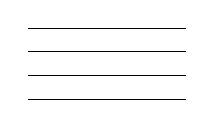
\begin{tikzpicture}
					\draw (0, 0) -- (2, 0);
					\draw (0, 0.3) -- (2, 0.3);
					\draw (0, 0.6) -- (2, 0.6);
					\draw (0, 0.9) -- (2, 0.9);
				\end{tikzpicture}
				\caption{Unit in TL$_4(\delta)$.}
				\label{fig:unit_temperley_lieb}
			\end{subfigure}
			\begin{subfigure}{0.49\textwidth}
				\centering
				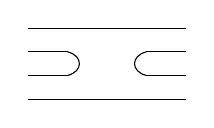
\begin{tikzpicture}
					\draw (0, 0) -- (2, 0);
					\draw (0, 0.3) -- (0.5, 0.3);
					\draw (0, 0.6) -- (0.5, 0.6);
					\draw (0.5, 0.3) .. controls (0.7, 0.35) and (0.7, 0.55) .. (0.5, 0.6);
					\draw (1.5, 0.3) -- (2, 0.3);
					\draw (1.5, 0.6) -- (2, 0.6);
					\draw (1.5, 0.3) .. controls (1.3, 0.35) and (1.3, 0.55) .. (1.5, 0.6);
					\draw (0, 0.9) -- (2, 0.9);
				\end{tikzpicture}
				\caption{Generator $U_2$ in TL$_4(\delta)$.}
				\label{fig:generator_temperley_lieb}
			\end{subfigure}
        	\end{figure}
        }

\subsection{Graded vector spaces}\label{section:graded_spaces}

	Similar to definition \ref{group:graded_ring} we can define the following:
	\newdef{Graded vector space}{\index{degree}\index{graded!vector space}
		Let $V_n$ be a vector space for all $n\in\mathbb{N}$. The vector space
		\begin{gather}
			\label{linalgebra:graded_vector_space}
			V = \bigoplus_{n\in\mathbb{N}} V_n
		\end{gather}
		is called a graded vector space. In fact one can replace $\mathbb{N}$ by any countable (finite or infinite) index set. For most operations however one requires the index set to be closed under addition operations. The index $n$ is often called the \textbf{degree} of the subspace $V_n$ in $V$.
	}
	
	\newdef{Graded algebra}{\index{graded!algebra}
		Let $V$ be a graded vector space with the additional structure of an algebra given by the multiplication $\star$. Then $V$ is a graded algebra if $\star$ maps $V^k\times V^l$ to $V^{k+l}$.
	}
	
	\newdef{Super vector space}{\index{super!vector space}
		A super vector space is defined as a $\mathbb{Z}_2$-graded vector space.
	}
	
	\begin{example}[Superalgebra]\index{super!algebra}\label{linalgebra:superalgebra}
		A $\mathbb{Z}_2$-graded algebra, i.e. there exists a decomposition
		\begin{gather}
			A = A_0\oplus A_1
		\end{gather}
		such that for all $i, j \mod 2$:
		\begin{gather}
			A_i\star A_j \subseteq A_{i+j}
		\end{gather}
	\end{example}
	
	\newdef{dg-algebra}{\index{dg-algebra}\label{linalgebra:dg_algebra}
		A differential graded algebra (often denoted by dg-algebra) is a graded algebra equipped with a differential of degree 1.
	}
	
	\newdef{Parity functor}{\index{parity}
		Consider the category $\mathbf{sVect}$ of super vector spaces. We can define the parity functor $\func{\Pi}{sVect}{sVect}$ as the functor which interchanges even and odd subspaces:
		\begin{align}
			(\Pi V)_0 &= V_1\\
			&\\
			(\Pi V)_1 &= V_0
		\end{align}
	}
	\newdef{Symmetric tensors}{
		Using the parity functor one can write the exterior algebra $\Lambda^\bullet(V)$ as the symmetric algebra $\text{Sym}^\bullet(\Pi V)$. In a similar way one can write the symmetric algebra on a super vector space $V=V_0\oplus V_1$ as $\text{Sym}^n(V)=\bigoplus_{p+q=n}\text{Sym}^p(V_0)\otimes\Lambda^q(V_1)$.
	}
        
\section[Linear maps]{Linear maps\footnote{Other names are \textbf{linear mapping} and \textbf{linear transformation}.}}

	\newdef{Injective}{\label{linalgebra:injective}
		A map $f:A\rightarrow B$ is called injective if the following condition is satisfied:
	    	\begin{gather}
		        \forall a, a'\in A:f(a)=f(a')\implies a=a'
		\end{gather}
	}
	\newnot{Injective map}{\[f:A\hookrightarrow B\]}
	\newdef{Surjective}{\label{linalgebra:surjective}
		A map $f:A\rightarrow B$ is called surjective if the following condition is satisfied:
	    	\begin{gather}
		        \forall b\in B, \exists a\in A:f(a) = b
		\end{gather}
	}
	\newnot{Surjective map}{\[f:A\twoheadrightarrow B\]}
	\newnot{Bijective map}{\[f:A\xrightarrow{\sim} B\qquad\text{or}\qquad f:A\cong B\]}
	\newnot{Isomorphic}{If two $K$-vector spaces $V, W$ are isomorphic we denote this by\[V\cong W\]}
	
	\begin{property}
		Let $V$ be finite-dimensional $K$-vector space. Let $f:V\rightarrow V$ be a linear map. The following statements are equivalent:
        	\begin{itemize}
            		\item $f$ is injective
			\item $f$ is surjective
                	\item $f$ is bijective
		\end{itemize}
	\end{property}

	\newdef{Automorphism}{\index{automorphism}\label{linalgebra:automorphism}
		\nomenclature[S_Aut]{$\text{Aut}(V)$}{Set of automorphisms (invertible endomorphisms) on a set $V$.}
	    	An isomorphism from $V$ to $V$ is called an automorphism\footnote{In some case also called a \textbf{linear operator}, but this terminology is also often used for a general linear map in \textit{operator theory}.}. The set of all automorphisms  on $V$, which is in fact a group, is denoted by $\text{Aut}(V)$.
	}
    
	\newdef{General linear group\footnotemark}{\index{general linear group}
		\nomenclature[S_GL]{GL$(V)$}{General linear group: group of all automorphisms on a vector space $V$.}
		\footnotetext{This group is isomorphic to the general linear group of invertible matrices, hence the similar name and notation. (See definition \ref{linalgebra:GL_matrices})}
	    	The set of all automorphisms $f:V\rightarrow V$ is called the general linear group and denoted by GL$_K(V)$ or GL$(V)$ when the base field is obvious.
	}

	\newdef{Rank}{\index{rank}\label{linalgebra:image_rank}
		The dimension of the image of a linear map is called the rank.
	}
	\newdef{Kernel}{\index{kernel}
	        The kernel of a linear map $f: V \rightarrow W$ is the following subset of $V$:
        	\begin{gather}
        		\text{ker}(f) = \{v\in V\ |\ f(v) = 0\}
	        \end{gather}
	}
	\newdef{Nullity}{\index{nullity}
		The dimension of the kernel is called the nullity.
	}
    
	\begin{theorem}
	    	A linear map $f:V\rightarrow W$ is injective if and only if $\text{ker}(f) = \{0\}$.
	\end{theorem}
	\begin{property}
	        Let $f:V\rightarrow W$ be a linear map. Let $U\leq V$. We have the following two properties of the restriction $f|_U$ of $f$ to $U$:
        	\begin{itemize}
			\item $\text{ker}\left(f|_U\right) = \text{ker}(f)\cap U$
        		\item $\text{im}\left(f|_U\right) \leq \text{im}(f)$
		\end{itemize}
	\end{property}
    
\subsection{Dimension}

        \begin{theorem}[Dimension theorem\footnotemark]\index{rank-nullity theorem}
		\footnotetext{Also called the \textbf{rank-nullity theorem}.}
		Let $f: V \rightarrow W$ be a linear map.
	        \begin{gather}
	                \label{linalgebra:dimension_theorem}
	                \dim(\text{\upshape im}(f)) + \dim(\text{\upshape ker}(f)) = \dim(\text{\upshape V})
	        \end{gather}
        \end{theorem}

        \begin{property}
		Two $K$-vector spaces are isomorphic if and only if they have the same dimension.
	\end{property}

\section{Inner product}\label{linalgebra:innerproduct}
	In the following section all vector spaces $V$ will be $\mathbb{R}$- or $\mathbb{C}$-vector spaces.
    
	\newnot{Inner product}{\index{inner!product}
		Let $v, w$ be two vectors in $V$. The map $\langle \cdot|\cdot \rangle:V\times V\rightarrow K$ is called an inner product on $V$ if it satisfies the following 3 properties:
		\begin{enumerate}
			\item \textbf{Conjugate symmetry:} $\langle v|w\rangle = \langle w|v\rangle^*$
			\item \textbf{Linearity in the first argument:} $\langle \lambda u + v|w\rangle = \lambda\langle u|w\rangle + \langle v|w\rangle$
			\item \textbf{Non-degeneracy: } $\langle v|v\rangle = 0 \iff v = 0$
			\item \textbf{Positive-definiteness} $\langle v|v\rangle \geq 0$
		\end{enumerate}
	}
	\remark{\index{Hermitian!form}
		\label{linalgebra:NDH_form}
    		Inner products are special cases of \textbf{non-degenerate Hermitian forms} which do not possses the positive-definiteness property.
	}

	\begin{result}
    		The first two properties have the result of conjugate linearity in the second argument:
    		\begin{equation}
			\langle f|\lambda g + \mu h\rangle = \overline{\lambda}\langle f|g \rangle + \overline{\mu}\langle f|h \rangle
		\end{equation}
	\end{result}
    
\subsection{Inner product space}
	
	\newdef{Inner product space\footnotemark}{
		\footnotetext{Sometimes called a \textbf{prehilbert space}.}
		A vector space equipped with an inner product $\langle\cdot|\cdot\rangle$ is called an inner product space.
	}

        \newdef{Metric dual\footnotemark}{\footnotetext{See also definition \ref{manifolds:flat_map}.}
        	Using the inner product (or any other non-degenerate Hermitian form) one can define the metric dual of a vector $v$ by the following map:
            \begin{equation}
            	\label{linalgebra:metric_dual}
            	L:V\rightarrow V^*:v\mapsto \langle v|\cdot \rangle
            \end{equation}
        }
        \newdef{Adjoint operator}{\index{Hermitian!adjoint}\index{self-adjoint}\label{linalgebra:adjoint_operator}
		Let $A$ be a linear operator on $V$. Let $v, w$ be two vectors in $V$. The \textit{Hermitian} adjoint of $A$ is defined as the linear operator $A^\dag$ that satisfies:
		\begin{equation}
			\langle A^\dag v, w\rangle = \langle v, Aw\rangle
		\end{equation}
		Alternatively one can define the adjoint using the metric dual $L(\cdot)$ as follows:
		\begin{equation}
			\boxed{A^\dag = L^{-1} \circ A^T \circ L}
		\end{equation}
		If $A = A^\dag$ then A is said to be \textbf{Hermitian} or \textbf{self-adjoint}.
	}
	
    \begin{result}
    	The Hermitian adjoint of a complex matrix $A\in\mathbb{C}^{m\times n}$ is given by:
        \begin{equation}
			A^\dag = \overline{A}^T
		\end{equation}
        where $\overline{A}$ denotes the complex conjugate of $A$ and $A^T$ the transpose of $A$.
    \end{result}
    
	The definition of an adjoint operator \ref{linalgebra:adjoint_operator} can be generalized to the case where $A^\dag$ is not unique (for example when $A$ is not globally defined) in the following way:
	\newdef{Conjugate operators}{
		Two operators $B$ and $C$ are said to be conjugate if:
		\begin{equation}
			\langle Bx, y\rangle = \langle x, Cy\rangle
		\end{equation}
	}
    
    \begin{example}\index{Lie!algebra}\index{isometry}
    	The Lie algebra associated with the group of isometries $\text{Isom}(V)$ of a non-degenerate Hermitian form satisfies following condition:
        \begin{equation}
        	\label{linalgebra:lie_isometry}
        	\langle Xv, w \rangle = -\langle v, Xw \rangle
        \end{equation}
        for all Lie algebra elements $X$. It follows that the Lie algebra consists of all anti-hermitian operators.
    \end{example}
    
\subsection{Orthogonality}\label{linalgebra:section:orthogonality}
	
	\newdef{Orthogonal}{
		Let $v, w \in V$. The vectors $v$ and $w$ are said to be orthogonal, denoted by $v\perp w$,  if they obey the following relation:
		\begin{equation}
			\label{linalgebra:orthogonal}
			\langle v|w \rangle = 0
		\end{equation}
		An orthogonal \textbf{system} is a set of vectors, none of them the null vector, that are mutually orthogonal.
	}
	\begin{property}
		Orthogonal systems are linearly independent.
	\end{property}
	
	\newdef{Orthonormal}{
		A set of vectors $\{v_n\}$ is said to be orthonormal if it is orthogonal and if all the elements $v_n$ obey the following relation:
		\begin{equation}
			\label{linalgebra:orthonormal}
			\langle v|v \rangle = 1
		\end{equation}
	}
        \newdef{Orthogonal complement\footnotemark}{\label{linalgebra:orthogonal_complement}Let $W$ be a subspace of $V$. The following subspace is called the orthogonal complement of $W$:
        	\begin{equation}
                W^\perp = \{v\in V\ |\ \forall w\in W:\langle v|w\rangle = 0\}
			\end{equation}
        }
        \footnotetext{$W^\perp$ is pronunciated as 'W-perp'.}
        
        	\begin{property}
		The inner-product is invariant under transformations between orthonormal bases.
	\end{property}
        
        \begin{property}
        	\label{linalgebra:W_W_perp_intersection}
			\begin{equation}
				W \cap W^\perp = \{0\}
			\end{equation}
		\end{property}
        \begin{property}
			Let $V$ be a finite-dimensional K-vector space. The orthogonal complement $W^\perp$ is a complementary subspace\footnotemark\ to W, i.e. $W\leq V$: $W\oplus W^\perp=V$.
		\end{property}
        \footnotetext{hence the name}
        \begin{result}
        	\label{linalgebra:perp_of_perp}
			Let $W\leq V$ where $V$ is a finite-dimensional K-vector space. We have the following relation:
            \begin{equation}
	            (W^\perp)^\perp = W
			\end{equation}
		\end{result}
    
    	\newdef{Orthogonal projection}{\index{projection}\label{linalgebra:orthogonal_projection}
    	Let $V$ be a finite-dimensional K-vector space. Let $W\leq V$. Let $w\in W$ and let $\{w_1, ..., w_k\}$ be an orthonormal basis of $W$. We define the projection of $v\in V$ on $W$ and $w\in W$ as follows:
        	\begin{equation}
				\text{proj}_W(v) = \sum_{i=1}^k\langle v|w_i \rangle w_i
			\end{equation}
            \begin{equation}
				\text{proj}_w(v) = \stylefrac{\langle v|w \rangle}{\langle w|w \rangle}w
			\end{equation}
        }
        \begin{property}\ 
			\begin{enumerate}
				\item $\forall w\in W:\text{proj}_W(w) = w$
                \item $\forall u\in W^\perp:\text{proj}_W(u) = 0$
			\end{enumerate}
		\end{property}
        
	\newmethod{Gram-Schmidt orthonormalisation}{
		Let $\{u_n\}$ be a set of linearly independent vectors. We can construct an orthonormal set $\{e_n\}$ out of $\{u_n\}$ in the following way:
		\begin{equation}
			\label{linalgebra:inner_product:gramm_schmidt}
			\begin{aligned}
				&w_1 = u_1&\\
				&w_2 = u_2 - \stylefrac{\langle u_2|w_1\rangle}{||u_2||^2}w_1&\\
				&\vdots&\\
				&w_n = u_n - \sum_{k = 1}^{n-1}\stylefrac{\langle u_n|w_k\rangle}{||u_n||^2}w_k&
			\end{aligned}\qquad
			\begin{aligned}
				&e_1 = \stylefrac{w_1}{||w_1||}&\\
				&e_2 = \stylefrac{w_2}{||w_2||}&\\
				&\vdots&\\
				&e_n = \stylefrac{w_n}{||w_n||}&
			\end{aligned}
		\end{equation}
	}
	
	\newdef{Householder transformation}{\index{Householder transformation}\label{linalgebra:householder_transformation}
		Let $v$ be an element of an inner product space $V$. The Householder transformation generated by $v$ is given by the linear map
		\begin{equation}
			\sigma_v:w\mapsto w - 2\frac{\langle w|v \rangle}{\langle v|v \rangle}v
		\end{equation}
		This transformation amounts to a reflection in the hyperplane orthogonal to $v$.
	}
        
\subsection{Angle}
	
	\newdef{Angle}{\index{angle}
		Let $v,w$ be elements of an inner product space $V$. The angle $\theta$ between $v$ and $w$ is defined as:
		\begin{equation}
			\label{linalgebra:angle}
			\boxed{\cos\theta = \stylefrac{\langle v|w \rangle}{||v||||w||}}
		\end{equation}
	}

\section{Matrices}
	
	\begin{notation}\label{linalgebra:matrix_set}
	        The set of all $m\times n$-matrices defined over the field K is denoted by $M_{m,n}(K)$. If $m=n$, the set is denoted by $M_n(K)$.
	\end{notation}
	
	\begin{property}[Dimension]\index{dimension}\label{linalgebra:dimension_of_matrix_space}
		The dimension of $M_{m,n}(K)$ is $mn$.
	\end{property}
    
	\newdef{Trace}{\index{trace}\label{linalgebra:trace}
	        Let $A = (a_{ij})\in M_n(K)$. We define the trace of $A$ as follows:
    		\begin{equation}
			\boxed{\operatorname{tr}(A) = \sum_{i=1}^na_{ii}}
		\end{equation}
	}
	\begin{property}\label{linalgebra:trace_commutative}
		Let $A, B\in M_n(K)$. We have the following properties of the trace:
	        \begin{enumerate}
        		\item $\text{tr}:M_n(K)\rightarrow K$ is a linear map
			\item $\text{tr}(AB) = \text{tr}(BA)$
			\item $\text{tr}(AB) \neq \text{tr}(A)\text{tr}(B)$
        		\item $\text{tr}(A^T) = \text{tr}(A)$
		\end{enumerate}
	\end{property}
    
	\newformula{Hilbert-Schmidt norm\footnotemark}{\index{Frobenius!norm}\index{Hilbert-Schmidt norm}
    		\footnotetext{Also called the \textbf{Frobenius norm}.}
    		The Hilbert-Schmidt matrix norm is given by following formula:
	        \begin{equation}
        		\label{linalgebra:hilbert_schmidt_norm}
        		||A||^2_{HS} = \sum_{i, j}|A_{ij}|^2 = \text{tr}(A^\dag A)
	        \end{equation}
        	If one identifies $M_{n}(\mathbb{C})$ with $\mathbb{C}^{2n}$ then this norm equals the standard Hermitian norm.
	}

	\newformula{Hadamard product}{\index{Hadamard!product}
    		The Hadamard product of two matrices $A, B\in M_{m\times n}(K)$ is defined as the entry-wise product:
        	\begin{equation}
        		(A\circ B)_{ij} = A_{ij}B_{ij}
        	\end{equation}
	}
    
	\newdef{General linear group}{\index{general linear group}\label{linalgebra:GL_matrices}
		\nomenclature[S_GLn]{GL$_n(K)$}{General linear group: group of all invertible $n$-dimensional matrices over the field $K$.}
	        The set of invertible matrices is called the general linear group and is denoted by GL$_n(K)$.
	}
	\begin{property}
		For all $A\in\text{GL}_n(K)$ we have:
	        \begin{itemize}
			\item $A^T\in\text{GL}_n(K)$
		        \item $\left(A^T\right)^{-1}=\left(A^{-1}\right)^T$
		\end{itemize}
	\end{property}
    
	\begin{property}\label{linalgebra:dim_columns_rows}
		Let $A\in M_{m,n}(K)$. Denote the set of columns as $\{A_1, A_2, ..., A_n\}$ and the set of rows as $\{R_1, R_2, ..., R_m\}$. The set of columns is a subset of $K^m$ and the set of rows is a subset of $K^n$. Furthermore we have:
		\[
			\dim(\text{span}(A_1, ..., A_n)) = \dim(\text{span}(R_1, ..., R_m))
		\]
	\end{property}
	
	\newdef{Rank of a matrix}{\index{rank}
		We can define the rank of matrix $A\in M_{m,n}(K)$ as follows:
		\begin{equation}
			\label{linalgebra:matrix_rank}
        			\text{rk}(A) := \dim(\text{span}(A_1, ..., A_n)) \overset{\ref{linalgebra:dim_columns_rows}}{=} \dim(\text{span}(R_1, ..., R_m))
		\end{equation}
	}
    
	\begin{property}\label{linalgebra:rank_properties}
	        The rank of a matrix has the folowing properties:
        	\begin{enumerate}
			\item Let $A\in M_{m,n}(K)$ and $B\in M_{n,r}(K)$. We have $\text{rk}(AB)\leq\text{rk}(A)$ and $\text{rk}(AB)\leq\text{rk}(A)$.
        		\item Let $A\in\text{GL}_n(K)$ and $B\in M_{n,r}(K)$. We have $\text{rk}(AB)=\text{rk}(B)$.
		        \item Let $A\in\text{GL}_n(K)$ and $B\in M_{r,n}(K)$. We have $\text{rk}(BA)=\text{rk}(B)$.
		\end{enumerate}
	\end{property}
	\begin{property}\label{linalgebra:dim_matrix_left_multiplication}
	        Let $A\in M_{m,n}(K)$. First define the following linear map:
        	\begin{equation}
			\label{linalgebra:matrix_left_multiplication}
        		\boxed{L_A:K^n\rightarrow K^m:v\mapsto Av}
		\end{equation}
	        This map has the following properties:
        	\begin{enumerate}
        		\item $\text{im}(L_A) = \text{span}(A_1, ..., A_n)$
			\item $\dim(\text{im}(L_A))=\text{rk}(A)$
		\end{enumerate}
	\end{property}
	\sremark{The second property is a direct consequence of the first one and definition \ref{linalgebra:matrix_rank}.}
    
\subsection{System of equations}

	\begin{theorem}\label{linalgebra:matrix_and_equations}
	        Let $AX=w$ with $A\in M_{m,n}(K)$, $w\in K^m$ and $X\in K^n$ be a system of $m$ equations in $n$ variables. Let $L_A$ be the linear map as defined in equation \ref{linalgebra:matrix_left_multiplication}. We then have the following properties:
        	\begin{enumerate}
			\item The system is false if and only if $w\not\in\text{im}(L_A)$.
        		\item If the system is not false, the solution set is an affine space. If $v_0\in K^n$ is a solution, then the solution set is given by: $L_A^{-1}(w)=v_0+\text{ker}(L_A)$.
		        \item If the system is homogeneous ($AX=0$), then the solution set is equal to $\text{ker}(L_A)$.
		\end{enumerate}
	\end{theorem}
	\begin{theorem}[Uniqueness]\label{linalgebra:rank_unique_solution}
	        Let $AX=w$ with $A\in M_n(K)$ be a system of $n$ equations in $n$ variables. If $\text{rk}(A)=n$, then the system has a unique solution.
	\end{theorem}
    
\subsection{Coordinates and matrix representations}

        \newdef{Coordinate vector}{\label{linalgebra:coordinate_vector}
        	Let $\mathcal{B} = \{b_1, ..., b_n\}$ be a basis of $V$. Let $v\in V$ such that $v=\sum_{i=1}^n\lambda_ib_i$. We define the coordinate vector of $v$ with respect to $\mathcal{B}$ as $(\lambda_1, ..., \lambda_n)^T$. The $\lambda_i$'s are called the \textbf{coordinates} of $v$ with respect to $\mathcal{B}$.
        }
        \newdef{Coordinate isomorphism}{\label{linalgebra:coordinate_isomorphism}
        	With the previous definition in mind we can define the coordinate isomorphism of $v$ with respect to $\mathcal{B}$ as follows:
        	\begin{equation}
			\boxed{\beta:V\rightarrow K^n:\sum_{i=1}^n\lambda_ib_i\mapsto(\lambda_1, ..., \lambda_n)^T}
		\end{equation}
        }
        
        \newdef{Matrix representation}{\label{linalgebra:matrix_representation}
        	Let $V$ be an $n$-dimensional K-vector space and $W$ an $m$-dimensional K-vector space. Let $f:V\rightarrow W$ be a linear map. Let $\mathcal{B}=\{b_1, ..., b_n\}, \mathcal{C} = \{c_1, ..., c_m\}$ be a basis for $V$, respectively $W$. The matrix representation of $f$ with respect to $\mathcal{B}$ and $\mathcal{C}$ can be derived as follows: For every $j\in\{1, ..., n\}$ we can write $f(b_j) = \sum_{i=1}^ma_{ij}c_i$, so with this in mind we can define the matrix $(a_{ij})\in M_{m,n}(K)$ as the matrix represenation of $f$.
        }
        \newnot{Matrix representation of a linear map}{
        	The matrix representation of $f$ with respect to $\mathcal{B}$ and $\mathcal{C}$ is denoted by $A_{f, \mathcal{B}, \mathcal{C}}$.
        }
        
        \newmethod{Construction of a matrix representation}{\label{linalgebra:method:matrix_representation}
        	From definition \ref{linalgebra:matrix_representation} we can see that $j$-th column of $A_{f, \mathcal{B}, \mathcal{C}}$ coincides with the coordinate vector of $f(b_j)$ with respect to $\mathcal{C}$. We use this relation to construct $A_{f, \mathcal{B}, \mathcal{C}}$ by writing for every $j\in\{1, ..., n\}$ the coordinate vector of $f(b_j)$ in the $j$-th column.
        }
        
        \begin{theorem}\label{linalgebra:theorem:matrix_representation}
		Let $(\lambda_1, ..., \lambda_n)^T$ be the coordinate vector of $v\in V$ with respect to $\mathcal{B}$. Let $(\mu_1, ..., \mu_m)^T$ be the coordinate vector of $f(v)$ with respect to $\mathcal{C}$. Then the following relation holds:
            	\begin{equation}
			\left(
			\begin{array}{c}
				\mu_1\\
				\vdots\\
				\mu_m
			\end{array}\right)
	                = A_{f, \mathcal{B}, \mathcal{C}}
        	        \left(\begin{array}{c}
				\lambda_1\\
				\vdots\\
				\lambda_n
			\end{array}\right)
		\end{equation}
	\end{theorem}
        
        \begin{theorem}\label{linalgebra:theorem:map_matrix_link}
		For every matrix $A\in M_{m,n}(K)$ there exists a linear map $f:V\rightarrow W$ such that $A_{f, \mathcal{B}, \mathcal{C}} = A$.
	\end{theorem}
        On the other hand we also have the following theorem:
        \begin{theorem}
		Let $f:K^n\rightarrow K^m$ be a linear map. There exists a matrix $A\in M_{m,n}(K)$ such that $f=L_A$.
	\end{theorem}
        \begin{theorem}
		Let $\beta$ and $\gamma$ be the coordinate isomorphisms with respect to respectively $\mathcal{B}$ and $\mathcal{C}$. From theorem \ref{linalgebra:theorem:matrix_representation} it follows that:
        	\begin{equation}
			\gamma(f(v)) = A_f\cdot\beta(v)
		\end{equation}
        	or alternatively
        	\begin{equation}
			\gamma\circ f = L_{A_f}\circ\beta
		\end{equation}
	\end{theorem}
        
        \begin{theorem}\label{linalgebra:theorem:matrix_composition_hom}
	        The map $\text{Hom}_K(V,W)\rightarrow M_{m,n}(K):f\mapsto A_f$ is an isomorphism and for every $f\in\text{Hom}_K(V,W)$ and $g\in \text{Hom}_K(W,U)$ we have:
		\begin{equation}
			A_{g\circ f} = A_gA_f
		\end{equation}
	\end{theorem}
	
	\begin{theorem}\label{linalgebra:theorem:matrix_composition_end}
	        The map $\text{End}_K(V)\rightarrow M_n(K):f\mapsto A_{f, \mathcal{B}, \mathcal{B}}$ is an isomorphism and for every $f,g\in\text{End}_K(V)$ we have:
        	\begin{equation}
			A_{g\circ f} = A_gA_f
		\end{equation}
	\end{theorem}
	
        \begin{theorem}\label{linalgebra:matrix_invertable_map}
	        Let $f\in\text{End}_K(V)$. Let $A_f$ be the corresponding matrix representation. The linear map $f$ is invertible if and only if $A_f$ is invertible. Furthermore, if $A_f$ is invertible, we have that \[\left(A_f\right)^{-1} = A_{f^{-1}}\] In other words, the following map is an isomorphism\footnotemark:
	        \begin{equation}
	        	\text{GL}_K(V)\rightarrow\text{GL}_n(K):f\mapsto A_f
	        \end{equation}
	        \footnotetext{Follows from theorem \ref{linalgebra:theorem:matrix_composition_end}.}
	\end{theorem}
        \remark{The sets GL$_K(V)$ and GL$_N(K)$ are groups. So the previous theorem states that the map $f\mapsto A_f$ is a group isomorphism.}
        
        \begin{theorem}
		Let $V = K^n$. Let $f\in V^*$. From construction \ref{linalgebra:method:matrix_representation} it follows that $A_f = (f(e_1), ..., f(e_n))\in M_{1,n}(K)$ with respect to the standard basis of $V$. This combined with theorem \ref{linalgebra:theorem:matrix_representation} gives:
	        \begin{equation}
			f(\lambda_1, ..., \lambda_n)^T = (f(e_1), ..., f(e_n))(\lambda_1, ..., \lambda_n)^T = \sum_{i=1}^nf(e_i)\lambda_i
		\end{equation}
        	or alternatively with $\{\varepsilon_1, ..., \varepsilon_n\}$ the dual basis to the standard basis of $V$:
	        \begin{equation}
        	    	\label{linalgebra:map_in_function_of_dual_basis}
			\boxed{f = \sum_{i=1}^nf(e_i)\varepsilon_i}
		\end{equation}
	\end{theorem}
        
        \begin{theorem}
		Let $f:V\rightarrow W$ be a linear map. Let $f^*:W^*\rightarrow V^*$ be the corresponding dual map. If $A_f$ is the matrix representation of $f$ with respect to $\mathcal{B}$ and $\mathcal{C}$, then the transpose $A_f^T$ is the matrix representation of $f^*$ with respect to the dual basis of $\mathcal{C}$ and the dual basis of $\mathcal{B}$.
	\end{theorem}
        
\subsection{Coordinate transforms}
        
        \newdef{Transition matrix}{\label{linalgebra:transition_matrix}
        	Let $\mathcal{B} = \{b_1, ..., b_n\}$ and $\mathcal{B}' = \{b_1', ..., b_n'\}$ be two bases of $V$. Every element of $\mathcal{B}'$ can be written as a linear combination of elements in $\mathcal{B}$:
        	\begin{equation}
        		b_j' = q_{1j}b_1 + ... + q_{nj}b_n
        	\end{equation}
	        The matrix $Q = (q_{ij})\in M_n(K)$ is called the transition matrix from the 'old' basis $\mathcal{B}$ to the 'new' basis $\mathcal{B}'$.}
        
        \begin{theorem}\label{linalgebra:theorem:transition_matrix}
		Let $\mathcal{B}, \mathcal{B}'$ be two basis of $V$. Let $Q$ be the transition matrix from $\mathcal{B}$ to $\mathcal{B}'$. We find the following statements:
	        \begin{enumerate}
			\item Let $\mathcal{C}$ be an arbitrary basis of $V$ with $\gamma$ the corresponding coordinate isomorphism. Define the following matrices:
        	        	\[
        	        		B=(\gamma(b_1), ..., \gamma(b_n))\quad\text{and}\quad B'=(\gamma(b_1'), ..., \gamma(b_n'))
        	        	\]
		                Then $BQ = B'$.
			\item $Q\in\text{GL}_n(K)$ and $Q^{-1}$ is the transition matrix from $\mathcal{B}'$ to $\mathcal{B}$.
                	\item Let $v\in V$ with $(\lambda_1, ..., \lambda_n)^T$ the coordinate vector with respect to $\mathcal{B}$ and $(\lambda_1', ..., \lambda_n')^T$ the coordinate vector with respect to $\mathcal{B}'$. Then:
                	\[
		                Q\left(
				\begin{array}{c}
					\lambda_1'\\
                			\vdots\\
			        	\lambda_n'
				\end{array}
                        	\right)
                        	=
		                \left(
                		\begin{array}{c}
					\lambda_1\\
                			\vdots\\
			        	\lambda_n
				\end{array}
                        	\right)
				\quad\text{and}\quad
                        	\left(
                        	\begin{array}{c}
					\lambda_1'\\
                        		\vdots\\
			        	\lambda_n'
				\end{array}
		                \right)
                	        =
                	        Q^{-1}\left(
                	        \begin{array}{c}
					\lambda_1\\
                		        \vdots\\
			                \lambda_n
				\end{array}
                        	\right)
			\]
		\end{enumerate}
	\end{theorem}
        
	\begin{theorem}\label{linalgebra:theorem:transition_matrix_representation}
        	Let $V,W$ be two finite-dimensional K-vector spaces. Let $\mathcal{B}, \mathcal{B}'$ be two bases of $V$ and $\mathcal{C}, \mathcal{C}'$ two bases of $W$. Let $Q, P$ be the transition matrices from $\mathcal{B}$ to $\mathcal{B}'$ and from $\mathcal{C}$ to $\mathcal{C}'$ respectively. Let $A=A_{f, \mathcal{B}, \mathcal{C}}$ and $A' = A_{f, \mathcal{B}', \mathcal{C}'}$. Then:
	        \begin{equation}
        	    	A' = P^{-1}AQ
        	\end{equation}
	\end{theorem}
        \begin{result}
		Let $f\in \text{End}_K(V)$ and let $Q$ be the transition matrix. From theorem \ref{linalgebra:theorem:transition_matrix_representation} it follows that:
            	\begin{equation}
	            	A'=Q^{-1}AQ
        	\end{equation}
	\end{result}

        \newdef{Matrix conjugation}{\index{conjugacy class}\index{matrix!conjugation}\label{linalgebra:conjugacy_class}
        	Let $A\in M_n(K)$. The set
        	\begin{equation}
	            	\{Q^{-1}AQ\ |\ Q\in\text{GL}_n(K)\}
        	\end{equation}
	        is called the conjugacy class\footnotemark\ of $A$. Another name for conjugation is \textbf{similarity transformation}.
        	\footnotetext{This is the general definition of conjugacy classes for groups. Furthermore, these classes induce a partitioning of the group.}
	}
        \begin{remark}
        	If $A$ is a matrix representation of a linear operator $f$, then the conjugacy class of $A$ consists out of every possible matrix representation of $f$.
        \end{remark}
        
        \begin{property}\index{trace}
        	From property \ref{linalgebra:trace_commutative} it follows that the trace of a matrix is invariant under similarity transformations:
        	\begin{equation}
            		\label{linalgebra:trace_invariance}
            		\boxed{\text{tr}(Q^{-1}AQ) = \text{tr}(A)}
	        \end{equation}
        \end{property}
        
        \newdef{Matrix congruence}{\index{matrix!congruence}\label{linalgebra:matrix_congruence}
        	Let $A, B\in M_n(K)$. If there exists a matrix $P$ such that
	        \begin{equation}
        	    	A = P^TBP
        	\end{equation}
	        then the matrices are said to be congruent.
        }
        \begin{property}
        	Every matrix congruent to a symmetric matrix is also symmetric.
        \end{property}
        
        \begin{theorem}\label{linalgebra:theorem:orthogonal_transition_matrix}
        	Let $(V, \langle .|. \rangle)$ be an inner-product space defined over $\mathbb{R}$ (or $\mathbb{C}$). Let $\mathcal{B}, \mathcal{B}'$ be two orthonormal bases of $V$ and let $Q$ be the transition matrix. Then $Q$ is orthogonal:
        	\begin{equation}
	        	Q^TQ = \mathbbm{1}_n
	        \end{equation}
	\end{theorem}

\subsection{Determinant}

    	\newdef{Minor}{
        	The $(i, j)$-th minor of $A$ is defined as:\[\det(A_{ij})\] where $A_{ij}\in M_{n-1}(K)$ is the matrix obtained by removing the $i$-th row and the $j$-th column from $A$.
	}
        \newdef{Cofactor}{
        	The cofactor $\alpha_{ij}$ of the matrix element $a_{ij}$ is equal to:\[(-1)^{i+j}\det(A_{ij})\]where $\det(A_{ij})$ is the minor as previously defined.
	}
        \newdef{Adjugate matrix}{\label{linalgebra:adjugate_matrix}
	        The adjugate matrix of $A\in M_n(K)$ is defined as follows:
	       	\begin{equation}
	            	\text{adj}(A) := \left(
	                \begin{array}{cccc}
				\alpha_{11}&\alpha_{21}&\dotsm&\alpha_{n1}\\
		                \alpha_{12}&\alpha_{22}&\dotsm&\alpha_{n2}\\
		                \vdots&\vdots&\vdots&\vdots\\
		                \alpha_{1n}&\alpha_{2n}&\dotsm&\alpha_{nn}\\
			\end{array}
        	        \right)
		\end{equation}
        	or shorter: $\text{adj}(A) = (\alpha_{ij})^T$.
        }
        \begin{remark*}
		It is important to notice that we have to transpose the matrix after the elements have been replaced by their cofactor.
	\end{remark*}
        
        \begin{property}\label{linalgebra:determinant_properties}
	        Let $A,B\in M_n(K)$. Denote the columns of $A$ as $A_1, \dotso, A_n$. We have the following properties of the determinant:
	        \begin{enumerate}
			\item $\det(A^T) = \det(A)$
	                \item $\det(AB) = \det(BA) = \det(A)\det(B)$
	                \item $\det(A_1, \dotso, A_i+\lambda A_i', \dotso, A_n) = \det(A_1, \dotso, A_i, \dotso, A_n) + \lambda\det(A_1, \dotso,A_i', \dotso, A_n)$ for all $A_i,A_i'\in M_{n,1}(K)$.
	                \item If two columns of $A$ are equal then $\det(A) = 0$.
	                \item $\det(A_{\sigma(1)},\dotso,A_{\sigma(n)}) = \text{sgn}(\sigma)\det(A_1,\dotso,A_n)$
	                \item The determinant can be evaluated as follows:
	                	\begin{equation}
					\det(A) = \sum_{i=1}^n(-1)^{i+k}a_{ik}\det(A_{ik})
				\end{equation}
		\end{enumerate}
		\end{property}
        
	\begin{theorem}\label{linalgebra:theorem:rank_det_equivalence}
        	Let $A\in M_n(K)$, the following statements are equivalent:
        	\begin{enumerate}
			\item $\det(A) \neq 0$
        	        \item $\text{rk}(A) = n$
        	        \item $A\in\text{GL}_n(K)$
		\end{enumerate}
	\end{theorem}
        \begin{theorem}\label{linalgebra:theorem:adjugate_matrix}
            For all $A\in M_n(K)$ we find $A\text{adj}(A) = \text{adj}(A)A = \det(A)I_n$.
	\end{theorem}
        \begin{formula}\label{linalgebra:theorem:determinant_inverse}
	        For all $A\in\text{GL}_n(K)$ we find:
		\begin{equation}
            		A^{-1} = \det(A)^{-1}\ \text{adj}(A)
            	\end{equation}
	\end{formula}
        
        An alternative definition of a $k\times k$-minor is: 
        \begin{definition}
		Let $A\in M_{m,n}(K)$ and $k\leq\min(m, n)$. A $k\times k$-minor of $A$ is the determinant of a $k\times k$-partial matrix obtained by removing $m-k$ rows and $n-k$ columns from $A$.
	\end{definition}
        \begin{theorem}
		Let $A\in M_{m,n}(K)$ and $k\leq\min(m, n)$. We find that $\text{rk}(A)\geq k$ if and only if $A$ contains a non-zero $k\times k$-minor.
	\end{theorem}
        
        \begin{theorem}
		Let $f\in\textup{End}_K(V)$. The determinant of the matrix representation of $f$ is invariant under basis transformations.
	\end{theorem}
	
        \newdef{Determinant of a linear operator}{\index{determinant}\label{linalgebra:operator_determinant}
        	The previous theorem allows us to unambiguously define the determinant of $f\in\textup{End}_K(V)$ as follows:
        	\[\det(f) := \det(A)\]
		where $A$ is some matrix representation of $f$.
        }

\subsection{Characteristic polynomial}

    	\begin{definition}[Characteristic polynomial\footnotemark]\index{characteristic!polynomial}\label{linalgebra:characteristic_polynomial}
		Let $V$ be a finite-dimensional K-vector space. Let $f\in \text{End}_K(V)$ be a linear operator with the matrix representation $A$ (with respect to some arbitrary basis). We then find:
		\begin{equation}
                	\chi_f(x) := \det(x\mathbbm{1}_n - A) \in K[x]
		\end{equation}
		is a monic polynomial of degree $n$ in the variable $x$ and the polynomial does not depend on the choice of basis.
		\footnotetext{This polynomial can also be used directly for a matrix $A$ as theorem \ref{linalgebra:theorem:map_matrix_link} matches every matrix $A$ with some linear operator $f$.}
	\end{definition}
        
        \begin{definition}[Characteristic equation\footnotemark]\index{characteristic!equation}
        	\footnotetext{This equation is sometimes called the \textbf{secular equation}.}
		The following equation is called the characteristic equation of $f$:
	        \begin{equation}
            		\label{linalgebra:characteristic_equation}
			\boxed{\chi_f(x) = 0}
		\end{equation}
	\end{definition}
        
        \begin{formula}\label{linalgebra:parts_of_characteristic_polynomial}
        	Let $A=(a_{ij})\in M_n(K)$ with characteristic polynomial: \[\chi_A(x) = x^n + c_{n-1}x^{n-1} + \dotso + c_1x + c_0\] We then have the following result:
        	\begin{equation}
			\begin{cases}
				c_0 = (-1)^n\det(A)\\
				c_{n-1} = -\text{tr}(A)
			\end{cases}
		\end{equation}
	\end{formula}
        
        \begin{theorem}[Cayley-Hamilton]\index{Cayley-Hamilton theorem}\label{linalgebra:cayley_hamilton}\
	        \begin{enumerate}
			\item Let $A\in\text{M}_n(K)$ with characteristic polynomial $\chi_A(x)$. We find the following relation:
		                \begin{equation}
					\chi_A(A) = A^n + \sum_{i=1}^{n-1}c_iA^i= 0
				\end{equation}
	                \item Let $f\in\textup{End}_K(V)$ with characteristic polynomial $\chi_f(x)$. We find that
		                \begin{equation}
					\chi_f(f) = f^n + \sum_{i=1}^{n-1}c_if^i= 0
				\end{equation}
		\end{enumerate}
	\end{theorem}
        \begin{result}
		From theorem \ref{linalgebra:minimal_polynomial_divisor} and the Cayley-Hamilton theorem it follows that the minimal polynomial $\mu_f(x)$ is a divisor of the characteristic polynomial $\chi_f(x)$.
	\end{result}
        
\subsection{Linear groups}\label{linalgebra:section:linear_groups}
        
        \newdef{Elementary matrix}{\label{linalgebra:elementary_matrix}An elementary matrix is a matrix of the following form:
        	\[\left(
                \begin{array}{cccc}
			1&0&\dotsm&0\\
        	        0&1&c_{ij}&0\\
                	\vdots&\vdots&\ddots&\vdots\\
	                0&0&\vdots&1
		\end{array}
		\right),
        	\left(
                \begin{array}{cccc}
			1&0&\dotsm&0\\
                	0&1&\dotsm&0\\
	                \vdots&c_{ij}&\ddots&\vdots\\
        	        0&0&\vdots&1
		\end{array}
		\right),\dotso\]
		i.e. equal to the sum of an identity matrix and a multiple of a matrix unit $U_{ij}, i\neq j$.
        }
        \newnot{Elementary matrix}{$E_{ij}(c)$ is the elementary matrix with element $c$ on the $i,j$-th position.}
        \begin{property}
        	We have the following property:
		\begin{equation}
			\det(E_{ij}(c)) = 1
		\end{equation}
		which implies that $E_{ij}(c)\in\text{GL}_n(K)$.
	\end{property}
        \begin{property}
		We find the following results concerning the multiplication by an elementary matrix:
	        \begin{enumerate}
			\item Left multiplication by an elementary matrix $E_{ij}(c)$ comes down to replacing the $i$-th row of the matrix with the $i$-th row plus $c$ times the $j$-th row.
                	\item Right multiplication by an elementary matrix $E_{ij}(c)$ comes down to replacing the $j$-th column of the matrix with the $j$-th column plus $c$ times the $i$-th column.
		\end{enumerate}
		\end{property}
        
        \begin{theorem}\label{linalgebra:theorem:elementary_matrices}
		Every matrix $A\in\text{GL}_n(K)$ can be written in the following way: \[A = SD\] where $S$ is a product of elementary matrices and $D=\text{diag}(1,\dotso,1,\det(A))$.
	\end{theorem}
        
        \newdef{Special linear group}{\label{linalgebra:special_linear_group}
        	The following subset of GL$_n(K)$ is called the special linear group:
		\begin{equation}
			\text{SL}_n(K) = \{A\in \text{GL}_n(K)\ |\ \det(A) = 1\}
		\end{equation}
        }
        \begin{theorem}
		Every $A\in\text{SL}_n(K)$ can be written as a product of elementary matrices.\footnote{This follows readily from theorem \ref{linalgebra:theorem:elementary_matrices}.}
	\end{theorem}
        
        \newdef{Orthogonal group}{\label{linalgebra:orthogonal_group}The orthogonal and special orthogonal group are defined as follows:
        	\begin{align}
			\text{O}_n(K) &= \{A\in \text{GL}_n(K)\ |\ AA^T = A^TA = I_n\}\nonumber\\
			\text{SO}_n(K) &= \text{O}_n(K)\cap \text{SL}_n(K)\nonumber
		\end{align}
        }
        \begin{property}\label{linalgebra:con_equivalence}
        	For orthogonal matrices, conjugacy \ref{linalgebra:conjugacy_class} and congruency \ref{linalgebra:matrix_congruence} are equivalent.
        \end{property}
        
        \newdef{Unitary group}{\label{linalgebra:unitary_group}\index{involution}
        	The unitary and special unitary group are defined as follows:
        	\begin{align}
			\text{U}_n(K, \sigma) &= \{A\in \text{GL}_n(K)\ |\ A\overline{A}^T = \overline{A}^TA = I_n\}\nonumber\\
			\text{SU}_n(K, \sigma) &= \text{U}_n(K)\cap \text{SL}_n(K)\nonumber
		\end{align}
		where $\sigma$ denotes the \textit{involution}\footnotemark\ $a^\sigma \equiv \overline{a}$.
		\footnotetext{An involution is an operator that is its own inverse: $f(f(x)) = x$.}
        }

	\begin{remark*}
		If $K=\mathbb{C}$ where the involution is taken to be the complex conjugate, the $\sigma$ is often ommited in the definition: U$_n(K)$ and SU$_n(K)$.
	\end{remark*}
	
	\newdef{Unitary equivalence}{
		Let $A, B$ be two matrices in M$_n(K)$. If there is a unitary matrix $U$ such that \[A = U^\dag BU\] then the matrices $A$ and $B$ are said to be \textbf{unitarily equivalent}.
	}
	
	\newdef{Symplectic group}{\index{symplectic!group}
		\nomenclature[S_SymA]{Sp$_n(K)$}{Symplectic group: Group of matrices preserving the canonical symplectic form over the field $K$.}
		Consider a vector space $V$ with an antisymmetric nonsingular matrix $\Omega$. The symplectic group Sp$_n(V, \Omega)$ is defined as follows:
		\begin{equation}
			\text{Sp}(V, \Omega) = \{A\in\text{GL}(V)\ |A^T\Omega A = \Omega\}
		\end{equation}
		On the real or complex numbers one can define the canonical \textbf{symplectic} matrix \[\Omega_{st} = \begin{pmatrix}0&-\mathbbm{1}\\\mathbbm{1}&0\end{pmatrix}\]
		The group of matrices that preserve this matrix are often denoted by Sp$_n(\mathbb{R})$ or Sp$_n(\mathbb{C})$.
	}
	\begin{property}
		Symplectic groups can only be defined on even-dimensional spaces because the defining matrix $\Omega$ can only be nonsingular if $n$ is even.
	\end{property}
	
	\newdef{Compact symplectic group}{
		\nomenclature[S_SymC]{Sp$(n)$}{Compact symplectic group: Sp$_{2n}(\mathbb{C})\cap\text{U}(2n)$.}
		The compact symplectic group is defined as follows:
		\begin{equation}
			\text{Sp}(n) = \text{Sp}_{2n}(\mathbb{C})\cap\text{U}(2n)
		\end{equation}
		This is in fact isomorphic to the \textit{quaternionic unitary group} in $n$ quaternionic dimensions.
	}
	\begin{example}
		For $n=1$ we find Sp$(1)\cong\text{SU}(2)$.
	\end{example}
	
\subsection{Matrix decomposition}

	\begin{method}[QR Decomposition]\index{QR!decompositon}
		Every square complex matrix $M$ can be decomposed as:
		\begin{equation}
			M = QR
		\end{equation}
		where $Q$ is unitary and $R$ is upper-triangular. The easiest (but not the most numerically stable) way to do this is by applying the Gram-Schmidt orthonormalisation process:
		
		Let $\{v_i\}_{i\leq n}$ be a basis for the column space of $M$. By applying the Gram-Schmidt process to this basis one obtains a new orthonormal basis $\{e_i\}_{i\leq n}$. The matrix $M$ can then be written as $QR$ where:
		\begin{itemize}
			\item $R$ is an upper-triangular matrix with entries $R_{ij} = \langle e_i|\text{col}_j(M) \rangle$ where col$_j(M)$ denotes the $j^{th}$ column of $M$.
			\item $Q = (a_1\cdots a_n)$ is the unitary matrix constructed by setting the $i^{th}$ column equal to the $i^{th}$ basis vector $a_i$ 
		\end{itemize}
	\end{method}
	\begin{property}
		If $M$ is invertible and if the diagonal elements of $R$ are required to have positive norm then the QR-decomposition is unique.
	\end{property}

\section{Eigenvectors}
	\begin{definition}[Eigenvector]
		A vector $v\in V\setminus\{0\}$ is called an \textbf{eigenvector} of the linear operator $f: V\rightarrow V$ if it satisfies the following equation:
        \begin{equation}
			f(v) = \lambda v
		\end{equation}
        Where $\lambda \in K$ is the \textbf{eigenvalue} belonging to $v$.
	\end{definition}
    \begin{definition}[Eigenspace]
		The subspace of $V$ consisting of the zero vector and the eigenvectors of an operator is called the \textbf{eigenspace} associated with that operator:
        \begin{equation}
			\text{ker}(\lambda\boldsymbol{1}_V - f)
		\end{equation}
	\end{definition}

	\begin{theorem}[Characteristic equation\footnotemark]
    	\label{linalgebra:theorem:eigenvalue_characteristic_equation}
    	Let $f\in\text{End}_K(V)$ be a linear operator. A scalar $\lambda\in K$ is an eigenvalue of $f$ if and only if it satisfies the characteristic equation \ref{linalgebra:characteristic_equation}.
	\end{theorem}
    \footnotetext{This theorem also holds for the eigenvalues of a matrix $A\in M_n(K)$.}
    
    \begin{theorem}
		A linear operator $f\in\text{End}_K(V)$ defined over an $n$-dimensional K-vector space $V$ has at most $n$ different eigenvalues.\footnote{This theorem also holds for a matrix $A\in M_n(K)$.}
	\end{theorem}
    
    \begin{method}[Finding the eigenvectors of a matrix $\mathbf{A}$]\leavevmode
		\begin{enumerate}
			\item First we find the eigenvalues $\lambda_i$ of $\mathbf{A}$ by applying theorem \ref{linalgebra:theorem:eigenvalue_characteristic_equation}.
            \item Then we find the eigenvector $v_i$ belonging to the eigenvalue $\lambda_i$ by using the following equation:
            \begin{equation}
				\label{linalgebra:eigenvectors:eigenspace}
                \left(\mathbf{A} - \lambda_i\mathbf{1}_V\right)v_i = 0
			\end{equation}
		\end{enumerate}
	\end{method}
    
    \subsection{Diagonalization}
    	\newdef{Diagonalizable operator}{An operator $f\in\text{End}_K(V)$ on a finite-dimensional K-vector space $V$ is diagonalizable if there exists a matrix representation $A\in M_n(K)$ of $f$ such that $A$ is a diagonal matrix.}
    
    	\begin{theorem}
			\label{linalgebra:theorem:diagonalizable_basis}
            A linear operator $f$ defined on a finite-dimensional K-vector space $V$ has a diagonal matrix as matrix representation if and only if the set of eigenvectors of $f$ is a basis of $V$.
		\end{theorem}
		
        \begin{theorem}
        	\label{linalgebra:theorem:diagonalizable_PQP}
            A matrix $A\in M_n(K)$ is diagonalizable if and only if there exists a matrix $P\in GL_n(K)$ such that $P^{-1}AP$ is diagonal.
        \end{theorem}
        \begin{result}\index{trace}
        	Using the fact that the trace of a linear operator is invariant under similarity transformations (see property \ref{linalgebra:trace_invariance}) we get following useful formula:
            \begin{equation}
            	\boxed{\text{tr}(f) = \sum_i\lambda_i}
            \end{equation}
            where $\{\lambda_i\}_{0\leq i\leq n}$ are the eigenvalues of $f$.
        \end{result}
        
        \begin{property}
        	\label{linalgebra:diagonalization_properties}
			Let $V$ be an $n$-dimensional K-vector space. Let $f\in \text{End}_K(V)$ be a linear operator. We find the following properties of the eigenvectors/eigenvalues of $f$:
            \begin{enumerate}
				\item The eigenvectors of $f$ belonging to different eigenvalues are linearly independent.
                \item If $f$ has exactly $n$ eigenvalues, $f$ is diagonalizable.
                \item If $f$ is diagonalizable, $V$ is the direct sum of the eigenspaces of $f$ belonging to the different eigenvalues of $f$.
			\end{enumerate}
		\end{property}
        
        \newdef{Multiplicity}{\index{multiplicity}
        	Let $V$ be a K-vector space. Let $f\in \text{End}_K(V)$ be a linear operator with characteristic polynomial\footnotemark:
        	\[\chi_f(x) = \prod_{i=1}^n(x-\lambda_i)^{n_i}\]
            We can define the following multiplicities:
            \begin{enumerate}
				\item The \textit{algebraic multiplicity} of an eigenvalue $\lambda_i$ is equal to $n_i$.
                \item The \textit{geometric multiplicity} of an eigenvalue $\lambda_i$ is equal to the dimension of the eigenspace belonging to that eigenvalue.
			\end{enumerate}
        }
        \footnotetext{We assume that the characteristic polynomial can be written in this form. This depends on the possibility to completely factorize the polynomial in $K$ (i.e. it has 'enough' roots in $K$). If not, $f$ cannot even be diagonalized. However, there always exists a field $F$ containing $K$, called a \textbf{splitting field}, where the polynomial has 'enough' roots.}
        \remark{The geometric multiplicity is always at least 1.}
        \begin{property}
			The algebraic multiplicity is always greater than or equal to the geometric multiplicity.
		\end{property}
        \begin{theorem}
			\label{linalgebra:theorem:diagonalizable_multiplicity}
            Let $f\in\text{End}_K(V)$ be a linear operator. $f$ is diagonalizable if and only if for every eigenvalue the algebraic multiplicity is equal to the geometric multiplicity.
		\end{theorem}
        
        \begin{property}\index{Hermitian}
        	\label{linalgebra:diagonalizable_hermitian}
			Every Hermitian operator $f\in\text{End}_K(\mathbb{C}^n)$ has the following properties:
            \begin{enumerate}
				\item All the eigenvalues of $f$ are real.
                \item Eigenvectors belonging to different eigenvalues are orthogonal.
                \item $f$ is diagonalizable and there always exists an orthonormal basis of eigenvectors of $f$.
			\end{enumerate}
		\end{property}
        
        \begin{property}\index{commutator}
			Let $A, B \in \text{End}_K(V)$ be two linear operators. If the commutator $[A, B] = 0$, then the two operators have a common eigenbasis.
		\end{property}
        
        \begin{theorem}[Sylvester's law of inertia]\index{Sylvester's law of inertia}
        	Let $S$ be a symmetric matrix. The number of positive and negative eigenvalues is invariant with respect to similarity transformations\footnotemark.
        \end{theorem}
        \footnotetext{Also with respect to conjugation, which are equivalent to similarity transformations according to property \ref{linalgebra:con_equivalence}.}

\section{Euclidean space}\index{Euclidean space}\index{Cartesian|seealso{Euclidean}}

    A finite-dimensional $\mathbb{R}$-vector space is called a \textbf{Euclidean space} or a \textbf{Cartesian space}.

    \begin{notation}
        When working in a Euclidean space the inner product $\langle v|w\rangle$ is often written as $v\cdot w$ or even $vw$.
    \end{notation}

    \newdef{Orientation}{\label{linalgebra:orientation}
        Let $\mathcal{B}, \mathcal{B}'$ be two ordered bases of $\mathbb{R}^n$ and let $Q$ be the transition matrix from $\mathcal{B}$ to $\mathcal{B}'$. If $\det(Q)>0$ then the bases are said to have the same orientation (or to be \textbf{consistently oriented}). If $\det(Q)<0$ then the bases are said to have an opposite orientation.
    }
    \begin{result}[Positive orientation]
        The previous definition imposes an equivalence relation on the set of bases of $\mathbb{R}^n$ such that the set of bases consists out of two equivalence classes. Take one class and call the bases in it \textbf{positively} (or \textbf{directly}) oriented. The bases in the other class are then said to be \textbf{negatively} (or \textbf{indirectly}) oriented.
    \end{result}
    \remark{It is convenient to take the standard basis $(e_1,\ldots,e_n)$ to be positively oriented.}

\section{Grassmanians}

    \newdef{Grassmannian}{\index{Grassmannian}\label{linalgebra:grassmannian}
        Let $V$ be a $K$-vector space. The set of all subspaces of dimension $k$ is called the Grassmannian $\text{Gr}(k, V)$.
    }
    \begin{property}\label{linalgebra:grassmannian_construction}
        GL$(V)$ acts transitively \ref{group:transitive} on all $k$-dimensional subspaces of $V$. From property \ref{group:transitive_action_property} it follows that the coset space GL$(V)/H_W$ for any stabilizer $H_W$ of some $W\in \text{Gr}(k, V)$ is isomorphic (as a set) to $\text{Gr}(k, V)$.
    \end{property}

    \newdef{Flag}{\index{flag}\index{signature}
        Let $V$ be a finite-dimensional vector space. A sequence of proper subspaces $V_1<\cdots<V_n$ is called a flag of $V$. The sequence $(\dim V_1, \ldots, \dim V_n)$ is called the \textbf{signature} of the flag. If for all $i$, $\dim V_i = i$, the flag is called \textbf{complete}.
    }

    \newdef{Flag variety}{\label{linalgebra:flag_manifold}
        The set of all flags of a given signature over a vector space $V$ is called the (generalized) flag variety (of that signature). If the underlying field is the field of real (or complex) numbers then the flag variety is a smooth (or complex) manifold\footnote{See chapter \ref{chapter:manifolds}.}, called the \textbf{flag manifold}.

        It should be noted that Grassmannians are a specific type of flag variaties.
    }

    \begin{property}[Parabolic subgroups]\index{Borel!subgroup}\index{parabolic subgroup}
        It can be shown that every flag variety has the structure of a homogeneous space: $Fl_{n,\underline{d}} \equiv \text{GL}(V) / P_{n, \underline{d}}$ (where $\underline{d}$ denotes the signature of the flags). These subgroups $P_{n,\underline{d}}$ are called \textbf{parabolic subgroups} (parabolic subgroups can always be obtained by taking intersections of maximal ones). The maximal parabolic subgroups are exactly those that define the Grassmannian variaties. The flag variety of all complete flags defines a the Borel subgroup $B_n$. It can be shown that every parabolic subgroup contains the Borel subgroup.
    \end{property}
\chapter{Vector \& Tensor Calculus}

References for this chapter are \cite{jeevanjee}.

\section{Nabla-operator}\label{vectorcalculus:nabla}
	
	\begin{definition}[Nabla]\index{nabla}
		\begin{equation}
        		\nabla\equiv\left(\pderiv{}{x}, \pderiv{}{y}, \pderiv{}{z}\right)
		\end{equation}
	\end{definition}

	Following formulas can be found by using basic properties of (vector) calculus.    
	\newformula{Gradient}{\index{gradient}
		\begin{equation}
			\label{vectorcalculus:gradient}
			\nabla V = \left(\pderiv{V_x}{x}, \pderiv{V_y}{y}, \pderiv{V_z}{z}\right)
		\end{equation}
	}
	\begin{formula}
		Let $\varphi(\vector{x})$ be a scalar field. The total differential $d\varphi$ can be rewritten as
	        \begin{equation}
			d\varphi = \nabla\varphi\cdot d\vec{r}
		\end{equation}
	\end{formula}
    
	\begin{property}
		The gradient of a scalar function $V$ is perpendicular to the level sets \ref{set:level_set} of $V$.
	\end{property}
    
	\newdef{Directional derivative}{\index{directional derivative}
	    	Let $\vec{a}$ be a unit vector. The directional derivative $\nabla_{\vector{a}}V$ is defined as the change of the function $V$ in the direction of $\vec{a}$:
	    	\begin{equation}
			\label{vectorcalculus:directional_derivative}
		        \nabla_{\vector{a}}V \equiv (\vec{a}\cdot\nabla)V
		\end{equation}
	}
	\begin{example}
		Let $\varphi(\vector{x})$ be a scalar field. Let $\vec{t}$ denote the tangent vector to a curve $\vec{r}(s)$ with $s$ natural parameter. The variation of the scalar field $\varphi(\vector{x})$ along $\vec{r}(s)$ is given by
	        \begin{equation}
			\pderiv{\varphi}{s} = \deriv{\vec{r}}{s}\cdot\nabla\varphi
		\end{equation}
	\end{example}
    
	\newdef{Conservative vector field}{\index{conservative}
	    	A vector field obtained as the gradient of a scalar function.
	}
	\begin{property}
		A vector field is conservative if and only if its line integral is path independent.
	\end{property}
	
	\newformula{Gradient of tensor}{
		Let $T$ be a tensor field with coordinates $x^i$. Let $\vector{e}^i(x^1, x^2, x^3)$ be a curvilinear orthogonal frame\footnote{See definition \ref{diff:frame}.}. The gradient of $T$ is defined as follows:
		\begin{equation}
			\nabla T = \pderiv{T}{x^i}\otimes\vector{e}^i
		\end{equation}
	}
	
	\newformula{Divergence}{\index{divergence}
		\begin{equation}
			\label{vectorcalculus:divergence}
			\nabla\cdot\vector{A} = \pderiv{A_x}{x} + \pderiv{A_y}{y} + \pderiv{A_z}{z}
		\end{equation}
	}
	\newdef{Solenoidal vector field}{\index{solenoidal}
		A vector field $\vector{V}(\vector{x})$ is said to be solenoidal if it satisfies:
		\begin{equation}
			\nabla\cdot\vector{V} = 0
		\end{equation}
		It is also known as a \textbf{divergence free vector field}.
	}

	\newformula{Rotor / curl}{\index{curl}\index{rotor|see{curl}}
		\begin{equation}
			\label{vectorcalculus:rotor}
			\nabla\times\vector{A} = \left(\pderiv{A_z}{y} - \pderiv{A_y}{z}, \pderiv{A_x}{z} - \pderiv{A_z}{x}, \pderiv{A_y}{x} - \pderiv{A_x}{y}\right)
		\end{equation}
	}
    
	\newdef{Irrotational vector field}{\index{irrotational}
		A vector field $\vector{V}(\vector{x})$ is said to be irrotational if it satisfies:
	    	\begin{equation}
	    		\nabla\times\vector{V} = 0
	    	\end{equation}
	}
	\begin{remark}
		All conservative vector fields are irrotational but irrotational vector fields are only conservative if the domain is simply-connected\footnote{See definition \ref{topology:simply_connected}.}
	\end{remark}

\subsection{Laplacian}

	\newdef{Laplacian}{\index{Laplace!operator}
		\begin{equation}
			\label{vectorcalculus:laplacian}
			\bigtriangleup V\equiv\nabla^2V = \mpderiv{2}{V}{x} + \mpderiv{2}{V}{y} + \mpderiv{2}{V}{z}
		\end{equation}
		\begin{equation}
			\label{vectorcalculus:vector_laplacian}
		        \nabla^2\vector{A} = \nabla\left(\nabla\cdot\vector{A}\right) - \nabla\times \left(\nabla\times\vector{A}\right)
		\end{equation}
	}
	\remark{Equation \ref{vectorcalculus:vector_laplacian} is called the \textbf{vector laplacian}.}
    
	\newformula{Laplacian in different coordinate systems}{\ 
	    	\begin{itemize}
		        \item Cylindrical coordinates $(\rho,\phi,z)$:
		    	        \begin{equation}
		        	    	\label{laplacian:cylindrical}
					\stylefrac{1}{\rho}\pderiv{}{\rho}\left(\rho\pderiv{}{\rho}\right) + \stylefrac{1}{\rho^2}\mpderiv{2}{}{\phi} + \mpderiv{2}{}{z}
				\end{equation}
		        \item Spherical coordinates $(r,\phi,\theta)$:
	        		\begin{equation}
					\label{laplacian:spherical}
                    			\stylefrac{1}{r^2}\left[\pderiv{}{r}\left(r^2\pderiv{}{r}\right) + \stylefrac{1}{\sin^2\theta}\mpderiv{2}{}{\phi} + \stylefrac{1}{\sin\theta}\pderiv{}{\theta}\left(\sin\theta\pderiv{}{\theta}\right)\right]
				\end{equation}
		\end{itemize}
	}
    
\subsection[Mixed properties]{Mixed properties\footnotemark}\label{vectorcalculus:mixed_properties}
	\footnotetext{See remark \ref{forms:vector_calculus} for a differential geometric approach.}
	
	\begin{equation}
		\label{vectorcalculus:rotor_of_gradient}
        	\nabla \times \left(\nabla V\right) = 0
	\end{equation}
	\begin{equation}
		\label{vectorcalculus:divergence_of_rotor}
	        \nabla \cdot \left(\nabla \times \vector{V}\right) = 0
	\end{equation}
    
	In Cartesian coordinates equation \ref{vectorcalculus:vector_laplacian} can be rewritten as follows:
	\begin{equation}
		\label{vectorcalculus:vector_laplacian_carthesian}
		\nabla^2\vector{A} = \left(\bigtriangleup A_x, \bigtriangleup A_y, \bigtriangleup A_z\right)
	\end{equation}
    
\subsection{Helmholtz decomposition}

	\newformula{Helmholtz decomposition}{\index{Helmholtz!decomposition}
		Let $\vector{P}$ be a vector field that decays rapidly (more than $1/r$) when $r\rightarrow\infty$. $\vector{P}$ can be written as follows:
	        \begin{equation}
			\label{vectorcalculus:helmholtz_decomposition}
		        \vector{P} = \nabla\times\vector{A} + \nabla V
		\end{equation}
	}

\section{Line integrals}\index{line!integral}\index{path!integral|see{line integral}}

	\newformula{Line integral of a continuous function}{\label{vectorcalculus:line_integral_scalar}
	    	Let $f:\mathbb{R}^3\rightarrow\mathbb{R}$ be a continuous function. Let $\Gamma$ be a piecewise smooth curve with parametrization $\vector{\varphi}(t), t\in [a, b]$. We define the line integral of $f$ over $\Gamma$ as follows:
        	\begin{equation}
			\int_\Gamma f(s)ds = \int_a^b f(\vector{\varphi}(t))||\vector{\varphi}'(t)||dt
		\end{equation}
	}
	\newformula{Line integral of a continuous vector field}{\label{vectorcalculus:line_integral_vector}
	    	Let $\vector{F}$ be a continuous vector field. Let $\Gamma$ be a piecewise smooth curve with parametrization $\vector{\varphi}(t), t\in [a, b]$. We define the line integral of $F$ over $\Gamma$ as follows:
        	\begin{equation}
			\int_\Gamma \vector{F}(\vector{s})\cdot d\vector{s} = \int_a^b \vector{F}(\vector{\varphi}(t))\cdot\vector{\varphi}'(t)dt
		\end{equation}
	}

\section[Integral theorems]{Integral theorems\footnotemark}
	\footnotetext{These theorems follow from the more general Stokes' theorem \ref{forms:theorem:stokes_theorem}.}

	\begin{theorem}[Fundamental theorem of calculus for line integrals]\index{Fundamental theorem!for line integrals}~\newline
	    	Let $\vec\Gamma:\mathbb{R}\rightarrow\mathbb{R}^3$ be a smooth curve.
		\begin{equation}
			\label{vectorcalculus:fundamental_theorem}
		        \int_{\Gamma(a)}^{\Gamma(b)}\nabla f(\vector{r})\cdot d\vector{r} = \varphi(\Gamma(b)) - \varphi(\Gamma(a))
		\end{equation}
	\end{theorem}
        
	\begin{theorem}[Kelvin-Stokes' theorem]\index{Stokes!Kelvin-Stokes theorem}
	    	\begin{equation}
			\label{vectorcalculus:stokes_theorem}
		        \oint_{\partial S}\vector{A}\cdot d\vector{l} = \iint_S \left(\nabla \times \vector{A}\right)dS
		\end{equation}
	\end{theorem}
    
	\begin{theorem}[Divergence theorem\footnotemark]\index{divergence!theorem}
	    	\footnotetext{Also known as \textit{Gauss's theorem} or the \textit{Gauss-Ostrogradsky theorem}.}
	    	\begin{equation}
			\label{vectorcalculus:divergence_theorem}
		        \oiint_{\partial V}\vector{A}\cdot d\vector{S} = \iiint_V \left(\nabla \cdot \vector{A}\right)dV
		\end{equation}
	\end{theorem}
	\begin{result}[Green's identity]\index{Green!identity}
	    	\begin{equation}
			\label{vectorcalculus:green_indentity}
		        \oiint_{\partial V}\left(\psi\nabla\phi - \phi\nabla\psi\right)\cdot d\vector{S} = \iiint_V \left(\psi\nabla^2\phi - \phi\nabla^2\psi\right) dV
		\end{equation}
	\end{result}
    
\section{Curvilinear coordinates}

	In this section the differential operators are generalized to curvilinear coordinates. To do this we need the scale factors as formally defined in equation \ref{diff:scale_factor}. Also there is no Einstein summation used, all summations are written explicitly.
    
	\newformula{Unit vectors}{
	    	\begin{equation}
			\pderiv{\vec{r}}{q^i} = h_i\hat{e}_i
		\end{equation}
	}
	\newformula{Gradient}{
	    	\begin{equation}
			\nabla V = \sum_{i=1}^3\stylefrac{1}{h_i}\pderiv{V}{q^i}\hat{e}_i
		\end{equation}
	}
	\newformula{Divergence}{
	    	\begin{equation}
			\nabla\cdot\vector{A} = \stylefrac{1}{h_1h_2h_3}\left(\pderiv{}{q^1}(A_1h_2h_3) + \pderiv{}{q^2}(A_2h_3h_1) + \pderiv{}{q^3}(A_3h_1h_2)\right)
		\end{equation}
	}
	\newformula{Rotor}{
	   	\begin{equation}
			(\nabla\times\vector{A})_i = \stylefrac{1}{h_jh_k}\left(\pderiv{}{q^j}(A_kh_k) - \pderiv{}{q^k}(A_jh_j)\right)
		\end{equation}
	        where $i\neq j\neq k$.
	}

\section{Tensor product}
\subsection{Tensor product}\index{tensor!product}
	\nomenclature[O_zsymbinten]{$X\otimes Y$}{Tensor product of the vector spaces $X$ and $Y$.}

	There are two possible ways to introduce the components of a tensor (on finite dimensional spaces). One way is to interpret tensors as multilinears maps another way is to interpret the components as expansion coefficients with respect to the tensor space basis.
    
	\begin{definition}\label{tensor:tensor_product}
    		The tensor product of vector spaces $V$ and $W$ is defined as\footnotemark\ the set of multilinear maps on the Cartesian product $V^*\times W^*$. Let $v, w$ be vectors in respectively $V$ and $W$. Let $g, h$ be vectors in the corresponding dual spaces. The tensor product of $v$ and $w$ is then defined as:
    		\footnotetext{\textit{isomorphic to} would be a better terminology. See the "universal property" \ref{tensor:prop:universal_property}. For a complete proof and explanation, see \cite{principal_bundles}.}
        	\begin{equation}
        		\boxed{(v\otimes w)(g, h) = v(g)w(h)}
	        \end{equation}
	\end{definition}
	
	\newdef{Tensor component}{
    		One way to define the tensor components is as follows: Let $\mathbf{T}$ be a tensor that takes $r$ vectors and $s$ covectors as input and returns a scalar. The different components are given by  $\mathbf{T}(e_i, ..., e_j, e^k, ...., e^l) = T_{i...j}^{\ \ \ \ k...l}$.
	}
    
	The following property can also be seen as the defining property of a tensor product (also in the case of infinite-dimensional spaces):
	\begin{uproperty}\index{universal!property}\label{tensor:prop:universal_property}
	   	Let $Z$ be a vector space. For every bilinear map $T:V\times W\rightarrow Z$ there exists a linear map $f:V\otimes W\rightarrow Z$ such that $T = f\circ\varphi$, where $\varphi$ is the bilinear map $V\times W\rightarrow V\otimes W$.
	\end{uproperty}
	\begin{result}
	    	The tensor product is unique up to a linear isomorphism. This results in the commutativity of the tensor product:
	    	\begin{equation}
			\label{tensor:prop:change}
	        	V\otimes W \cong W\otimes V
		\end{equation}
		where the isomorphism is explicitly given by:
	        \begin{equation}
	        	v(f) \equiv f(v)
	        \end{equation}
	        for all $v\in V$ and $f\in V^*$.
	\end{result}
    
	\begin{notation}[Tensor power]\index{tensor!power}
	    	\begin{equation}
	    		V^{\otimes n} = \underbrace{V\otimes...\otimes V}_{n\text{ copies}}
	    	\end{equation}
	\end{notation}
	\begin{remark}
	    	More generally, the tensor product of $r$ copies of $V$ and $s$ copies of $V^*$ is the vector space $\mathcal{T}^r_s(V) = V^{\otimes r}\otimes V^{*\otimes s}$. These tensors are said to be of \textbf{type} $(r, s)$.
	\end{remark}
	
	\begin{remark}
		Generally the space $\mathcal{T}^1_1V$ is only isomorphic to the space $\text{End}(V^*)$. The isomorphism is given by the map $\hat{T}:V^*\rightarrow V^*:\omega\mapsto\mathbf{T}(\cdot, \omega)$ for every $\mathbf{T}\in\mathcal{T}^1_1V$. Furthermore the spaces $\mathcal{T}^0_1V$ and $V^*$ are isomorphic.
		
		For finite-dimensional vector spaces the space $\mathcal{T}^1_1V$ is also isomorphic to $\text{End}(V)$ (see property \ref{linalgebra:dual_space_dimension}) and the space $\mathcal{T}^1_0V$ will also be isomorphic to $V$ itself.
	\end{remark}
	\begin{definition}
	    	The scalars (elements of the base field $K$) are by definition the $(0,0)$ tensors.
	\end{definition}

	\begin{adefinition}\index{tensor!type}\label{tensor:type}
    		The tensor space $\mathcal{T}^r_s(V)$ is spanned by the elements
    		\[\underbrace{e_i\otimes...\otimes e_j}_{r\text{ basis vector}}\otimes\underbrace{\varepsilon^k\otimes...\otimes \varepsilon^l_{\textcolor{white}{a}}}_{s\text{ dual basis vectors}}\]
    		where the operation $\otimes$ satisfies following properties:
        	\begin{enumerate}
        		\item Associativity: $u\otimes(v\otimes w) = u \otimes v\otimes w$
		        \item Multilinearity: $a(v\otimes w) = (av)\otimes w = v\otimes (aw)$ and $v\otimes (u+w) = v\otimes u + v\otimes w$
	        \end{enumerate}
	        The expansion coefficients in this basis are written as $T^{i...j}_{\ \ \ \ k...l}$
	\end{adefinition}

	\newprop{Dimension of tensor product}{
	    	From the previous construction it follows that the dimension of $\mathcal{T}^r_s(V)$ is equal to $rs$.
	}
    
    	We now have to proof that the values of the tensor operating on $r$ basis vectors and $s$ basis covectors are equal to the corresponding expansion coefficients:
      	\begin{proof}
        	Let $\mathbf{T} = T_{i...j}^{\ \ \ \ k...l}e^i\otimes...\otimes e^j\otimes e_k\otimes...\otimes e_l$. Applying \ref{tensor:tensor_product} and using the definition of the dual vectors \ref{linalgebra:dual_basis_2} we have:
		\[
            	\begin{array}{ccl}
            		\mathbf{T}(e_a, ..., e_b, \varepsilon^m, ..., \varepsilon^n) &=& T_{i...j}^{\ \ \ \ k...l}e^i(e_a)...e^j(e_b)e_k(e^m)...e_l(e^n)\\
                	&=& T_{i...j}^{\ \ \ \ k...l}\delta_a^i...\delta_b^j\delta_k^m...\delta_l^n\\
                	&=& T_{a...b}^{\ \ \ \ m...n}
	        \end{array}
		\]
		This is exactly the same result as the one we get by applying the first definition.\qed
      	\end{proof}
      	
      	\newdef{Tensor algebra}{\index{tensor!algebra}\label{tensor:tensor_algebra}
      		The tensor algebra over a vector space $V$ is defined as follows:
      		\begin{equation}
      			T(V) = \bigoplus_{k\geq0}V^{\otimes k}
      		\end{equation}
      	}

\subsection{Quotient space}

	On infinite-dimensional spaces there exists a more general definition (that coincides with the previous one on finite-dimensional spaces\footnote{This can be checked using the universal property.}):
	\begin{construct}[Tensor product]\index{tensor!product}
		Consider two vector spaces $V, W$ over a field $K$. First construct the free vector space $F(V\times W)$ over $K$. Then construct the subspace $N$ of $F(V\times W)$ spanned by the following elements:
		\begin{itemize}
			\item $(v+v', w) - (v, w) - (v', w)$
			\item $(v, w+w') - (v, w) - (v, w')$
			\item $(kv, w) - k(v, w)$
			\item $(v, lw) - l(v, w)$
		\end{itemize}
		where $v\in V, w\in W$ and  $k,l\in K$. The tensor product $V\otimes W$ is then given by the quotient $F(V\times W)/N$.
	\end{construct}

\section{Transformation rules}

	Let the basis for $V$ transform as $e_i' = A^j_{\ i}e_j$ and $e_i = B^j_{\ i}e_j'$. Because the basis transformation should be well-defined, the operators $A$ and $B$ are each other's inverses: $B = A^{-1}$.

	\begin{definition}[Contravariant]
		A tensor component that transforms by the following rule is called contravariant:
	        \begin{equation}
			\label{tensorcalculus:contravariant}
		        v^i = A^i_{\ j}v'^j
		\end{equation}
	\end{definition}
    
	\begin{definition}[Covariant]
		A tensor component that transforms by the following rule is called covariant:
	        \begin{equation}
			\label{tensorcalculus:covariant}
		        p_i = B^j_{\ i}\ p'_j
		\end{equation}
	\end{definition}
    
	\begin{example}[Mixed tensor]
		As an example of a mixed tensor we give the transformation formula for the mixed third-order tensor $T_{\ ij}^k$:
	        \[
	        	T_{\ ij}^k = A^k_{\ w}B^u_{\ i}B^v_{\ j}T_{\ \ uv}'^w
	        \]
	\end{example}

	\begin{theorem}[Quotient rule]
		Assume we have an equation such as $K_iA^{jk} = B_i^{\ jk}$ or $K_i^{\ j}A_{jl}^{\ \ k} = B_{il}^{\ \ k}$ with $A$ and $B$ two known tensors\footnotemark. The quotient rule asserts the following: "If the equation of interest holds under all transformations, then $K$ is a tensor of the indicated rank and covariant/contravariant character".
		\footnotetext{This rule does not necessarily hold when $B = 0$ as transformations rules are not defined for the null-tensor.}
	\end{theorem}
	\sremark{This rule is a useful substitute for the "illegal" division of tensors.}

\section{Tensor operations}
\subsection{General operations}

	\newdef{Contraction}{\index{contraction}
	    	Let $A$ be a tensor of type $(n, m)$. Setting a sub- and superscript equal and summing over this index gives a new tensor of type $(n-1, m-1)$. This operation is called the contraction of $A$. It is given by the evaluation map
	    	\begin{equation}
	    		\label{tensor:contraction}
	    		V\otimes V^*:e_i\otimes e^j\mapsto e^j(e_i)
	    	\end{equation}
	}
    
	\newdef{Direct product}{\index{direct product}
	    	Let $A$ and $B$ be two random tensors (both rank and co-/contravariancy). The tensor constructed by the componentwise multiplication of $A$ and $B$ is called the direct product of $A$ and $B$.
	}
	\begin{example}
		Let $A_{\ k}^i$ and $B_{\ lm}^j$ be two tensors. The direct product is equal to: \[C_{\ k\ lm}^{i\ j} = A_{\ k}^iB_{\ lm}^j\]
	\end{example}
    
	\newformula{Operator product}{
    		It is also possible to combine operators working on different vector spaces so to make them work on the tensor product space. To do this we use following definition:
        	\begin{equation}
	        	\label{tensor:operator_product}
			\boxed{(\hat{A}\otimes\hat{B})(v\otimes w) = (\hat{A}v)\otimes(\hat{B}w)}
	        \end{equation}
	}
	\begin{remark*}
	    	Consider an operator $\hat{A}$ working on a space $V_1$. When working with a combined space $V_1\otimes V_2$ the corresponding operator is in fact $\hat{A}\otimes\mathbbm{1}$ but it is often still denoted by $\hat{A}$ in physics.
	\end{remark*}
	
	\begin{notation}
		Consider a tensor with two indices $T_{ij}$. The antisymmetric part is written as follows:
		\begin{equation}
			T_{[ij]} = \frac{1}{2}\left(T_{ij} - T_{ji}\right)
		\end{equation}
	\end{notation}
	
\subsection{Determinant}

	\newdef{Form}{\index{form}
		An $n$-form is a totally antisymmetric element $\omega\in\mathcal{T}^0_nV$.
	}
	\newdef{Volume form}{\index{volume!form}
		A form of rank $\dim V$ is also called a \textbf{top form} or \textbf{volume form}.
	}

	\newdef{Determinant}{\index{determinant}
		Let $V$ be finite-dimensional with basis $\{e_i\}_{i\leq n}$. Let $\varphi$ be a tensor in $\mathcal{T}^1_1V\cong\text{End}(V)$ and let $\omega$ be a volume form. The determinant of $\varphi$ is then defined as:
		\begin{equation}
			\det\varphi = \frac{\omega(\varphi(e_1), ..., \varphi(e_n))}{\omega(e_1, ..., e_n)}
		\end{equation}
		This definition is well-defined, i.e. it is independent of the choice of volume form and basis. Furthermore it coincides with definition \ref{linalgebra:operator_determinant}.
		
		One should note that the determinant is only well-defined for $(1,1)$-tensors. Although other types of tensors can also be represented as matrices, definition \ref{linalgebra:operator_determinant} would not be independent of a choice of basis anymore. An alternative concept can be defined using principal bundles and more precisely frame bundles (see section \ref{manifolds:section:principal_bundles}).
	}
	
	\begin{result}
		\begin{equation}
			\omega(e_1, ..., e_{i-1}, X, e_{i+1}, ..., e_n) = X_i
		\end{equation}
	\end{result}

\subsection{Differentiation}
	
	\begin{property}
		\begin{equation}
        		\nabla\cdot(\vector{A}\otimes\vector{B}) = (\nabla\cdot\vector{A})\vector{B}+(\vector{A}\cdot\nabla)\vector{B}
		\end{equation}
	\end{property}    
    
\subsection{Levi-Civita tensor}
	
	\newdef{Levi-Civita tensor}{\index{Levi-Civita!symbol}
    		Let $e^i$ be the dual vector to $e_i$. In $n$ dimensions, we define the Levi-Civita tensor as follows:
    		\begin{equation}
        		\label{tensor:levi_civita_symbol}
			\boldsymbol{\varepsilon} = \varepsilon_{12...n}e^1\otimes e^2\otimes...\otimes e^n
        	\end{equation}
		where
        	\[
        	\varepsilon_{i...n} = 
        	\left\{
        	\begin{array}{rcl}
			1&\qquad&\text{if }(i...n)\text{ is an even permutation of }(12...n)\\
                	-1&\qquad&\text{if }(i...n)\text{ is an odd permutation of }(12...n)\\
	                0&\qquad&\text{if any of the indices occurs more than once}
		\end{array}
        	\right.
		\]
	}
	\begin{remark}\label{tensor:remark:levi_civita_symbol}
		The Levi-Civita symbol is not a tensor, but a pseudotensor. This means that the sign changes under reflections (or any transformation with determinant $-1$). To turn it into a proper tensor one should multiply it by a factor $\sqrt{g}$ where $g$ is the determinant of the metric.
    	\end{remark}

	\newformula{Cross product}{
		By using the Levi-Civita symbol, we can define the $i$-th component of the cross product\footnotemark\ as follows:
		\footnotetext{Following from remark \ref{tensor:remark:levi_civita_symbol} we can see that the cross product is in fact not a vector, but a pseudovector.}
		\begin{equation}
			\boxed{(\vector{v}\times\vector{w})_i = \varepsilon_{ijk}v_jw_k}
		\end{equation}
	}

\subsection{Complexification}

	\newdef{Complexification}{\index{complexification}\label{tensor:complexification}
		Let $V$ be a real vector space. The complexification of $V$ is defined as the following tensor product:
		\begin{equation}
			V^{\mathbb{C}} = V\otimes\mathbb{C}
		\end{equation}
		As such this is still a real vector space. However we can turn this space into a complex vector space by generalizing the scalar product as follows:
		\begin{equation}
			\alpha(v\otimes\beta) = v\otimes(\alpha\beta)
		\end{equation}
		for all $\alpha,\beta\in\mathbb{C}$.
	}
	\begin{property}
		By noting that every element $v_{\mathbb{C}}\in V^{\mathbb{C}}$ can be written as \[v_{\mathbb{C}} = (v_1\otimes1) + (v_2\otimes i)\] we can decompose the complexification as follows:
		\begin{equation}
			V^{\mathbb{C}} \cong V\oplus iV
		\end{equation}
	\end{property}

\section{Symmetrized tensors}
\subsection{Symmetric tensors}

	\begin{notation}
		\nomenclature[S_SnV]{$S^n(V)$}{Space of symmetric rank $n$ tensors over a vector space $V$.}
		The space of symmetric $(n, 0)$ tensors is denoted by $S^n(V)$. The space of symmetric $(0,n)$ tensors is denoted by $S^n(V^*)$.
	\end{notation}
    
\subsection{Antisymmetric tensors}

	\newdef{Antisymmetric tensor}{\index{antisymmetry}
		Tensors that change sign under the interchange of any two indices.
	}
	\begin{notation}\label{tensor:not:antysimmetric_space}
		\nomenclature[S_zsymLambda]{$\Lambda^n(V)$}{Space of antisymmetric rank $n$ tensors over a vector space $V$.}
		The space of antisymmetric $(0,n)$ tensors is denoted by $\Lambda^n(V^*)$. The space of antisymmetric $(n, 0)$ tensors is denoted by $\Lambda^n(V)$.
	\end{notation}

	\begin{remark*}\index{bivector}\index{blade}
    		Elements of $\Lambda^2(V)$ are also known as \textbf{bivectors}. Elements of $\Lambda^k(V)$ are generally known as $k$-\textbf{blades}.
	\end{remark*}
    
	\begin{property}
    		Let $n = \dim(V)$. $\Lambda^r(V)$ equals the null-space for all $r\geq n$.
	\end{property}
    
\subsection{Wedge product}

	\begin{formula}[Antisymmetrization]
		Let $\{P_i\}_i$ be the set of all permutations of the sequence $(1, ..., k)$.
		\begin{equation}
			\label{tensors:antisymmetrization}
			\text{Alt}(e_1\otimes...\otimes e_k) = \sum_i \sgn(P_i)e_{P_i(1)}\otimes...\otimes e_{P_i(k)}
		\end{equation}
	\end{formula}

	\newdef{Wedge product}{\index{wedge!product}
		Let $\{e_i\}_{1\leq i\leq \dim(V)}$ be a basis for $V$.
		\begin{equation}
			\label{tensor:wedge_product}
    			e_1 \wedge ... \wedge e_k = \text{Alt}(e_1\otimes...\otimes e_k)
    		\end{equation}
		From this definition it immediately follows that the wedge product is (totally) antisymmetric.
	}
    
	\begin{construct}
    		Let $\{e_i\}_{1 \leq i\leq \dim(V)}$ be a basis for $V$. It is clear from the definition \ref{tensor:wedge_product} that a basis for $\Lambda^r(V)$ is given by
		\[
			\{e_{i_1}\wedge...\wedge e_{i_r}\ :\ \forall k: 1\leq i_k \leq \dim(V)\}
		\]
		The dimension of this space is given by:
		\begin{equation}
			\label{tensor:wedge_dimension}
			\dim\Lambda^r(V) = \binom{n}{r}
		\end{equation}
		From the antisymmetry it follows that for $r>\dim(V)$ the spaces $\Lambda^r(V)$ are zero.
	\end{construct}
	\begin{remark}
		For $k=0$, the above construction is not useful, so we just define $\Lambda^0(V) = \mathbb{R}$.
	\end{remark}
	
	\begin{formula}
		Let $v\in\Lambda^r(V)$ and $w\in\Lambda^m(V)$.
		\begin{equation}
			v\wedge w = \frac{1}{r!m!}\text{Alt}(v\otimes w)
		\end{equation}
		where the antisymmetrization operator $\text{Alt}$ is defined in equation \ref{tensors:antisymmetrization}.
	\end{formula}
    
    \newformula{Levi-Civita symbol}{\index{Levi-Civita!symbol}
    	The Levi-Civita tensor in $n$ dimensions as introduced in \ref{tensor:levi_civita_symbol} can now be rewritten more concisely as:
        \begin{equation}
        	\boldsymbol{\varepsilon} = e_1\wedge...\wedge e_n
        \end{equation}
    }
    
    \begin{formula}\index{cross!product}
    	In 3 dimensions there exists an important isomorphism $J:\Lambda^2(\mathbb{R}^3)\rightarrow\mathbb{R}^3$:
        \begin{equation}
		\label{tensor:wedge_to_cross}
	        	J(\lambda)^i = \frac{1}{2}\varepsilon^i_{\ jk}\lambda^{jk}
        \end{equation}
        where $\lambda\in\Lambda^2(\mathbb{R}^3)$.

	Looking at the definition of the cross product \ref{linalgebra:cross_product}, we can see that $\vector{v}\times\vector{w}$ is actually the same as $J(\vector{v}\wedge\vector{w})$. One can thus use the wedge product to generalize the cross product to higher dimensions.
    \end{formula}
    
    \begin{example}
    	Let $A, B$ and $C$ be three vectors in $V$. Now consider following expression:
        \[
        	(C\wedge B)(L(A), \cdot)
        \]
        where $L(A)$ is the metric dual of $A$ (see \ref{linalgebra:metric_dual}). Evaluating this formula using the properties of the wedge and tensor products leads to the well known BAC-CAB rule of triple cross products:
        \[
        	(C\cdot A)B - (B\cdot A)C
        \]
    \end{example}
    
\subsection{Exterior algebra}
	
	\newdef{Exterior power}{\index{exterior!power}\index{form}
		In the theory of exterior algebras, the space $\Lambda^k(V)$ is often called the $k^{th}$ exterior power of $V$. Its elements are called (exterior) \textbf{$k$-forms}.
	}
	\newdef{Exterior algebra}{\index{exterior!algebra}\index{Grassmann!algebra}\label{tensor:exterior_algebra}
		We can define a graded vector space\footnotemark\ $\Lambda^*(V)$ as follows:
		\[
			\Lambda^*(V) = \bigoplus_{k\geq0}\Lambda^k(V)
		\]
		Then we can turn this graded vector space into a graded algebra by taking the wedge product as the multiplication:
		\[
			\wedge:\Lambda^k(V)\times\Lambda^l(V)\rightarrow \Lambda^{k+l}(V)
		\]
		This algebra is called the exterior algebra or \textbf{Grassmann algebra} over $V$.
		\footnotetext{See definition \ref{linalgebra:graded_vector_space}.}
	}
	
	\newadef{$\dag$}{\label{tensor:adef_exterior_algebra}
    		Let $T(V)$ be the tensor algebra over the vector space $V$, i.e.
	    	\begin{equation}
			T(V) = \bigoplus_{k\geq0} V^{\otimes k}
		\end{equation}
		The exterior algebra over $V$ is generally defined as the quotient of $T(V)$ by the two-sided ideal $I$ generated by $\{v\otimes v:v\in V\}$.
	}
	
	\begin{property}
		The exterior algebra is both a unital associative algebra with unit element $1\in\mathbb{R}$ and a coalgebra. Furthermore it is also commutative in the graded sense (see \ref{group:graded_commutativity}).
	\end{property}
	
	\begin{property}
		The graded commutativity implies that the wedge product of any odd exterior form with itself is identically 0. The wedge product of an even exterior form with itself vanishes if and only if the form can be decomposed as a product of 1-forms. 
	\end{property}
	
\subsection{Hodge star}

	It follows from equation \ref{tensor:wedge_dimension} that the spaces $\Lambda^k(V)$ and $\Lambda^{n-k}(V)$ have the same dimension, so there exists an isomorphism between them. This map is given by the Hodge star $\ast$. However this map can only be defined independent of the choice of (ordered) basis if we restrict ourselves to vector spaces equipped with a non-degenerate Hermitian form \ref{linalgebra:NDH_form}.

	When equipped with an inner product and hence an orthonormal basis $\{e_i\}$, every finite-dimensional vector space admits a canonical volume form given by Vol$ = e_1\wedge...\wedge e_n$. This will be the convention adopted in the remainder of this section.

	\newdef{Orientation}{\index{orientation}\label{tensor:orientation}
		Let Vol be the choice of volume form on the vector space $V$. From the definition of a volume form it follows that every other $\dim(V)$-blade is a scalar multiple of $\text{Vol}$. Hence the choice of volume form induces an orientation on $V$: if the scalar $r>0$ then the orientation is said to be \textbf{positive}, if $r<0$ then the orientation is \textbf{negative}.
	}
	
	\begin{formula}[Inner product]\index{inner!product}
		Let $V$ be equipped with an inner product $\langle\cdot,\cdot\rangle$. Then we can define an inner product on $\Lambda^k(V)$ by:
		\begin{equation}
			\label{tensor:wedge_inner_product}
			\boxed{\langle v_1\wedge...\wedge v_k | w_1\wedge...\wedge w_k \rangle_k = \det(\langle v_i, w_j\rangle)}
		\end{equation}
		For an orthogonal basis, this formula factorises into:
		\begin{equation}
			\langle v_1\wedge...\wedge v_k | w_1\wedge...\wedge w_k \rangle_k = \langle v_1|w_1 \rangle\cdots \langle v_k|w_k \rangle
		\end{equation}
	\end{formula}
	\newdef{Hodge star}{\index{Hodge star}
		The Hodge star $\ast: \Lambda^k(V)\rightarrow\Lambda^{n-k}(V)$ is defined as the isomorphism such that for all $\omega\in\Lambda^k(V)$ and $\rho\in\Lambda^{n-k}(V)$ we have the following equality:
		\begin{equation}
			\label{tensor:hodge_star}
			\omega\wedge\rho = \langle\ast\omega, \rho\rangle_{n-k}\text{Vol}(V)
		\end{equation}
		where $\langle\cdot,\cdot\rangle$ is the inner product \ref{tensor:wedge_inner_product} on $\Lambda^{n-k}(V)$. Furthermore, this isomorphism is unique.
		\begin{proof}
			Because $\omega\wedge\rho$ is an element of $\Lambda^n(V)$ it is a scalar multiple of $\text{Vol}(V)$. This implies that it can be written as \[c(\rho)\text{Vol}(V)\] The map $c : \Lambda^{n-k}(V)\rightarrow\mathbb{R}:\rho\mapsto c(\rho)$ is a linear map and thus a continuous map, so we can apply Riesz' representation theorem to identify $c$ with a unique element $\ast\omega\in\Lambda^{n-k}(V)$ such that \[c(\rho) = \langle\ast\omega, \rho\rangle_{n-k}\]
		\qed
		\end{proof}
	}
	
	\begin{formula}
		Let $\{e_i\}_{i\leq n}$ be a positively oriented ordered orthonormal (possibly in a Lorentzian signature) basis for $V$. An explicit formula for the Hodge star is given by the following construction. Let $\{i_1, ..., i_k\}$ and $\{j_1 ,...,j_{n-k}\}$ be two complementary index sets with increasing subindices. Let $\omega = e_{i_1}\wedge...\wedge e_{i_k}$.
		\begin{equation}
			\label{tensor:explicit_hodge_star}
			\boxed{\ast\omega =\sgn(\tau)\prod_{m = 1}^{n-k}\langle e_{j_m}|e_{j_m} \rangle e_{j_1}\wedge...\wedge e_{j_{n-k}}}
		\end{equation}
		where $\tau$ is the permutation that maps $e_{i_1}\wedge...\wedge e_{i_k}\wedge e_{j_1}\wedge...\wedge e_{j_{n-k}}$ to $\text{Vol}(V)$.
	\end{formula}
	
	\begin{result}
		\label{tensor:hodge_star_vectorcalculus}
		Consider three vectors $u, v, w\in\mathbb{R}^3$.
		\begin{align}
			\ast(v\wedge w) &= v\times w \label{tensor:cross_by_hodge_star}\\
			\ast(v\times w) &= v\wedge w\\
			\ast(u\wedge v\wedge w) &= u\cdot(v\times w)
		\end{align}
	\end{result}
	\begin{remark}
		Formula \ref{tensor:wedge_to_cross} is an explicit evaluation of the first equation \ref{tensor:cross_by_hodge_star}.
		\begin{proof}
			The sign $\sgn(\tau)$ can be written using the Levi-Civita symbol $\varepsilon_{ijk}$ as defined in \ref{tensor:levi_civita_symbol}. The factor $\frac{1}{2}$ is introduced to correct for the double counting due to the contraction over both the indices $j$ and $k$.
		\end{proof}
	\end{remark}
	
	\begin{property}
		Consider an inner product space $V$, then
		\begin{equation}
			\boxed{\ast\ast\ \omega = (-1)^{k(n-k)}\omega}
		\end{equation}
		In $n=4$ this leads to $\ast\ast\omega = \omega$ which means that the Hodge star is an involution in 4-dimensional inner product spaces.
	\end{property}
	
	\newdef{Self-dual}{\index{dual!self-dual}
		Let $V$ be a 4-dimensional inner product space. Consider $\omega\in\Lambda^2(V)$. Then $\omega$ is said to be self-dual if $\ast\omega = \omega$. Furthermore every $v\in\Lambda^2(V)$ can be uniquely decomposed as the sum of a self-dual and an anti-self-dual 2-form.
	}
	
\subsection{Grassmann numbers}

	Although this section does not really belong to the chapter about tensors, we have included it here as it is an application of the concept of exterior algebras. The concept of Grassmann numbers (or variables) is used in QFT when performing calculations in the fermionic sector.
	
	\newdef{Grassmann numbers}{\index{Grassmann!number}\label{tensor:grassmann_number}
		Let $V$ be a complex vector space spanned by a set of generators $\theta_i$. The Grassmann algebra with Grassmann variables $\theta_i$ is the exterior algebra over $V$. The wedge symbol of Grassmann variables is often ommitted when writing the product: $\theta_i\wedge\theta_j \equiv \theta_i\theta_j$.
	}
	\begin{remark}
		Furthermore, from the anti-commutativity it follows that we can regard the Grassmann variables as being non-zero square-roots of zero.
	\end{remark}
	
	\begin{property}
		Consider a one-dimensional Grassmann algebra. When constructing the polynomial ring $\mathbb{C}[\theta]$ generated by $\theta$, we see that, due to the anti-commutativity, $\mathbb{C}[\theta]$ is spanned only by $1$ and $\theta$. All higher degree terms vanish because $\theta^2 = 0$. This implies that the most general polynomial over a one-dimenisonal Grassmann algebra can be written as
		\begin{equation}
			p(\theta) = a + b\theta
		\end{equation}
	\end{property}
	
	\begin{definition}\index{DeWitt!convention}
		We can equip the exterior algebra $\Lambda$ with Grassmann variables $\theta_i$ with an involution similar to that on $\mathbb{C}$:
		\begin{equation}
			(\theta_i\theta_j...\theta_k)^* = \theta_k...\theta_j\theta_i
		\end{equation}
		Elements $z\in\Lambda$ such that $z^* = z$ are called \textbf{(super)real}, elements such that $z^* = -z$ are called \textbf{(super)imaginary}. This convention is called the \textit{DeWitt} convention.
	\end{definition}

\chapter{Normed Spaces}

	In this chapter the term "linear operator", which was previously reserved for vector space automorphisms, is now used instead of "linear map". This was done to keep the vocabulary in track with that of the standard literature on Banach spaces and operator spaces.
	
	For a revision of inner product spaces see section \ref{linalgebra:innerproduct}.

\section{Banach spaces}

	\newdef{Topological vector space}{\index{vector!space}
		\nomenclature[A]{TVS}{Topological vector space}
		A topological vector space (TVS) over a base field $K$ is a vector space for which the addition and scalar multiplication over $K$ are continuous.
	}
	
	\newdef{Weak topology}{\index{topology!weak}\label{hilbert:weak_topology}
		The initial topology on a TVS with respect to its dual. 
	}

	\newdef{Norm}{\index{norm}
    		Let $V$ be a TVS over a field $K$. A function $||\vec{v}||:V\rightarrow[0,+\infty[$ is called a norm if it satisfies following conditions:
		\begin{itemize}
			\item \textbf{Non-degeneracy:} $||\vec{v}|| = 0 \iff \vec{v} = 0$
			\item \textbf{Homogeneity:} $||a\vec{v}|| = |a|||\vec{v}||$ for all scalars $a\in K$
			\item \textbf{Triangle equality (subadditivity):} $||\vec{v} + \vec{w}|| \leq ||\vec{v}|| + ||\vec{w}||$
		\end{itemize}
	}
	\remark{
		A norm $||\cdot||$ clearly induces a metric\footnotemark\ by setting $d(x,y) = ||x-y||$.
	}
	\footnotetext{See definition \ref{topology:metric}.}
    
	\newdef{Normed vector space}{
    		A TVS equipped with a norm $||\cdot||$.
	}
	\newdef{Banach space}{\index{Banach!space}\label{linalgebra:banach_space}
	    	A normed vector space that is complete\footnote{See condition \ref{topology:cauchy_sequence}.} in the norm-topology.
	}
	
	\begin{property}
		The topological (continuous) dual of a Banach space is also a Banach space.
	\end{property}
	\newdef{Reflexive space}{
		A Banach space $V$ that coincides with its double (topological) dual, i.e. $V = (V^*)^*$.
	}
	\begin{property}
		Every finite-dimensional Banach spaces is reflexive. This follows from property \ref{linalgebra:dual_space_dimension}.
	\end{property}
	
	\begin{property}
		Let $(x_n)$ be a Cauchy sequence in a normed space $V$. Then $(||x_n||)$ is a convergent sequence in $\mathbb{R}$. This implies that every Cauchy sequence in a normed space is bounded.
	\end{property}

	\begin{property}
		Let $X$ be a TVS. Every linear map $\varphi:\mathbb{K}^n\rightarrow X$ is continuous.
	\end{property}
	\begin{property}
		Let $X$ be a finite-dimensional normed vector space. Every linear bijection $\varphi:\mathbb{K}^n\rightarrow X$ is a homeomorphism.
	\end{property}
	\begin{result}
		Two finite-dimensional normed vector spaces with the same dimension are homeomorphic. It follows that all metrics on a finite-dimensional normed vector space are equivalent.
	\end{result}

	\begin{theorem}[Open mapping theorem\footnotemark]\index{open mapping theorem}
		\footnotetext{Sometimes called the \textit{Banach-Schauder} theorem.}
		Let $f:V\rightarrow W$ be a continuous linear operator between two Banach spaces. If $f$ is surjective then it is also open.
	\end{theorem}
	
	\begin{theorem}[Hahn-Banach theorem]\index{Hahn-Banach}
		Let $V$ be a Banach space. Let $f:V\rightarrow\mathbb{R}$ be a sublinear map, i.e. a map that is both subadditive and positive-homogeneous, and let $\phi:U\rightarrow\mathbb{R}$ be a linear map dominated by $f$, defined on a linear subspace $U\subset V$. Then there exists a linear extension $\psi:V\rightarrow\mathbb{R}$ of $\phi$ that is dominated by $f$ on all of $V$.
	\end{theorem}

\section{Hilbert space}

	\newdef{Hilbert space}{\index{Hilbert!space}\label{hilbert:hilbert_space}
		A vector space that is both a Banach space and an inner product space (where the norm is induced by the inner product).
	}

	\begin{example}
		Let $f, g \in \mathcal{L}^2([a,b], \mathbb{C})$, the inner product of $f$ and $g$ is defined as:
		\begin{equation}
			\label{hilbert:inner_product}
		        \boxed{\langle f|g\rangle = \int_a^bf^*(x)\overline{g(x)}dx}
		\end{equation}
	\end{example}
	\remark{
		See section \ref{lebesgue:section:hilbert_space} for a more formal treatment of this subject.
	}
    
	\begin{formula}
		It is also possible to define an inner product with respect to a weight function $\phi(x)$:
		\begin{equation}
			\label{hilbert:weighted_inner_product}
			\int_a^bf^*(x)g(x)\phi(x)dx
		\end{equation}
		Using this formula it is possible to define orthogonality with respect to a weight function.
	\end{formula}
    
\subsection{Inner products and norms}
	\begin{formula}
		Let $V$ be an inner product space. A norm on $V$ can be induced by the inner product in the following way:
		\begin{equation}
			\label{linalgebra:inner_product:norm}
			||v||^2 = \langle v|v \rangle
		\end{equation}
		However not every norm induces an inner product. Only norms that satisfy the parallellogram law \ref{linalgebra:parallellogram_law} induce an inner product. This inner product can be recovered through the polarization identity \ref{linalgebra:polarization_identity} (see below).
	\end{formula}
	
	\begin{property}[Cauchy-Schwarz inequality]\index{Cauchy-Schwarz}\label{linalgebra:theorem:cauchy_schwarz}
		\begin{equation}
			\boxed{|\langle v|w\rangle| \leq ||v||\ ||w||}
		\end{equation}
		where the equality holds if and only if $v$ and $w$ are linearly dependent.
	\end{property}
	\begin{result}
		The Cauchy-Schwarz inequality can be used to prove the triangle inequality. Together with the properties of an inner product this implies that an inner product space is also a normed space.
	\end{result}
	
	\begin{formula}[Parallellogram law]\index{parallellogram law}
		\begin{equation}
			\label{linalgebra:parallellogram_law}
			||v+w||^2 + ||v-w||^2 = 2(||v||^2 + ||w||^2)
		\end{equation}
	\end{formula}
	\begin{formula}[Polarization identity]\index{polarization!identity}
		\begin{equation}
			\label{linalgebra:polarization_identity}
			4 \langle v|w \rangle = ||v+w||^2 - ||v-w||^2 + i\left(||v+iw||^2 - ||v-iw||^2\right)
		\end{equation}
	\end{formula}
	\begin{formula}[Pythagorean theorem]\index{Pythagorean theorem}
		In an inner product space the triangle equality reduces to the well-known Pythagorean theorem for orthogonal vectors $v, w$:
		\begin{equation}
			\label{linalgebra:pythagorean_theorem}
			||v+w||^2 = ||v||^2 + ||w||^2
		\end{equation}
		This formula can be extended to any set of orthogonal vectors $x_1, ..., x_n$:
		\begin{equation}
			\boxed{\left\lVert\sum_{i=1}^nx_i\right\rVert^2 = \sum_{i=1}^n||x_i||^2}
		\end{equation}
	\end{formula}

\subsection{Generalized Fourier series}

	\begin{property}[Bessel's inequality]\index{Bessel!inequality}
		First of all we have following general equality for orthonormal vectors $x_1, ..., x_n$ and complex scalars $a_1, ..., a_n$:
		\begin{equation}
			\left\lVert x - \sum_{i=1}^n a_ix_i\right\rVert^2 = ||x||^2 - \sum_{i=1}^n|\langle x, x_i\rangle|^2 + \sum_{i=1}^n|\langle x, x_i\rangle - a_i|^2
		\end{equation}
		This expression becomes minimal for $a_i = \langle x, x_i\rangle$ (last term becomes 0). This leads to Bessel's inequality:
		\begin{equation}
			\label{norm:bessels_inequality}
			\boxed{\sum_{i=1}^n|\langle x, x_i\rangle|^2 \leq ||x||^2}
		\end{equation}
	\end{property}
	\begin{result}\index{Fourier!generalized series}
		The sum in \ref{norm:bessels_inequality} is bounded for all $n$, so the series $\sum_{i=1}^{+\infty}$ converges for all $x$. This implies that the sequences $(\langle x, x_n\rangle)$ belongs to the space $l^2$ of square-summable sequences.
	\end{result}
	
	This result does however not imply that the generalized Fourier series $\sum_{i=1}^{+\infty}\langle x, x_i\rangle x_i$ converges to $x$. The following theorem gives a necessary and sufficient condition for the convergence.
	\begin{theorem}
		Let $\mathcal{H}$ be a Hilbert space. Let $(x_n)$ be an orthonormal sequence in $\mathcal{H}$ and let $(a_n)$ be a sequence in $\mathbb{C}$. The expansion $\sum_{i=1}^{+\infty}a_ix_i$ converges in $\mathcal{H}$ if and only if $(a_n)\in l^2$. Furthermore the expansion satisfies following equality:
		\begin{equation}
			\left\lVert\sum_{i=1}^{+\infty}a_ix_i\right\rVert^2 = \sum_{i=1}^{+\infty}|a_i|^2
		\end{equation}
		As we noted the sequence $(\langle x, x_n\rangle)$ belongs to $l^2$ so the generalized Fourier series converges of $x\in\mathcal{H}$ converges in $\mathcal{H}$.
	\end{theorem}
	\begin{remark}
		Although the convergence of the generalized Fourier series of $x\in\mathcal{H}$ can be established using previous theorem, it does not follow that the expansion converges to $x$ itself. We can merely say that the Fourier expansion is the best approximation of $x$ with respect to the norm on $\mathcal{H}$.
	\end{remark}
    
\subsection{Complete sets}

	\newdef{Complete set}{\index{complete!set}
		Let $\{e_i\}_{i\in I}$ be a set (possibly a sequence) of orthonormal vectors in an inner product space $V$. This set is said to be complete if every vector $x\in V$ can be expressed as follows:
		\begin{equation}
			x = \sum_{i\in I}\langle x, x_i\rangle x_i
		\end{equation}
		This implies that a complete set is a basis for the vector space.
	}
	Another characterization is the following.
	\begin{adefinition}
		A complete set of orthonormal vectors is a set $S\subset V$ such that we cannot add another vector $w$ to it satisfying:
		\begin{equation}
			\forall v_i\in S: \langle v_i, w\rangle = 0\qquad\land\qquad  w\neq0
		\end{equation}
	\end{adefinition}
	
	\begin{property}
		For complete sequences $(x_n)$ the inequality of Bessel \ref{norm:bessels_inequality} becomes an equality. Furthermore, the generalized Fourier series with respect to the complete sequence is unique.
	\end{property}
	
	Using previous property we can prove the following theorem due to Parceval.
	\begin{theorem}[Parceval]\index{Parceval}
		Let $(x_n)$ be a complete sequence in a Hilbert space $\mathcal{H}$. Every vector $x\in\mathcal{H}$ has a unique Fourier series representation $\sum_{i=1}^{+\infty}a_ix_i$ where the Fourier coefficients $(a_i)$ belong to $l^2$ and the inequality of Bessel is an equality.
		
		Conversely if the inequality of Bessel becomes an equality for every $x\in\mathcal{H}$ then the sequence $(x_n)$ is complete.
	\end{theorem}
	
	\begin{property}
		A sequence $(x_n)$ in a Hilbert space $\mathcal{H}$ is complete if and only if $\langle x, x_i\rangle = 0$ for all $x_i$ implies that $x=0$.
	\end{property}

\subsection{Orthogonality and projections}

	The basic notions on orthogonality in inner product space can be found in section \ref{linalgebra:section:orthogonality}.

	\begin{property}
		Let $S$ be a subset (not necessarily a subspace) of a Hilbert space $\mathcal{H}$. The orthogonal complement $S^\perp$ is closed in $\mathcal{H}$.
	\end{property}
	\begin{result}
		The previous property implies that the orthogonal complemement of some arbitrary subset of a Hilbert space is a Hilbert space itself.
	\end{result}
	
	\begin{theorem}[Projection theorem]
		\label{linalgebra:theorem:projection_theorem}
		Let $H$ be a Hilbert space and $K\leq H$ a complete subspace. For every $h\in H$ there exists a unique $h'\in K$ such that $h-h'$ is orthogonal to every $k\in K$, i.e $h-h'\in K^\perp$.
	\end{theorem}
	\remark{
		An equivalent definition for the unique $h'\in K$ is $||h-h'|| = \inf\{||h-k||:k\in K\}$.
	}
	\begin{result}
		It follows that given a complete (or closed) subspace $S$ the Hilbert space $\mathcal{H}$ can be decomposed as $\mathcal{H} = S\oplus S^\perp$.
	\end{result}
	
	\newdef{Trace}{\index{trace}
		Let $\mathcal{H}$ be a Hilbert space wih orthogonal basis ${e_k}$. Given a bounded linear operator $S\in\mathcal{B}(\mathcal{H})$ we define its trace by the following formula:
		\begin{equation}
			\label{hilbert:trace}
			\text{tr}(S) = \sum_k\langle |S|e_k, e_k\rangle
		\end{equation}
	}

\subsection{Separable Hilbert spaces}

	The definition of separable spaces in the sense of point-set topology is given in \ref{topology:separable}. An equivalent definition for Hilbert spaces is the following.
	\newadef{Separable Hilbert space}{
		A Hilbert space is separable if it contains a complete sequence of orthonormal vectors.
	}
	\begin{result}
		Using the Gram-Schmidt method it follows from previous definition that every finite-dimensional Hilbert space is separable.
	\end{result}

	The following theorem shows that (up to an isomorphism) there are only 2 distinct types of separable Hilbert spaces.
	\begin{theorem}
		Let $\mathcal{H}$ be separable. If $\mathcal{H}$ is finite-dimensional with dimension $n$ then it is isometrically isomorphic to $\mathbb{C}^n$. If $\mathcal{H}$ is infinite-dimensional then it is isometrically isomorphic to $l^2$.
	\end{theorem}
	\begin{property}
		Every orthogonal subset of a separable Hilbert space is countable.
	\end{property}

\subsection{Linear functionals}

	\begin{property}
		Let $f$ be a continuous linear functional. Then two possibilities arise:
		\begin{enumerate}
			\item $\dim(\ker f)^\perp=0$ if $f\equiv0$.
			\item $\dim(\ker f)^\perp=1$
		\end{enumerate}
	\end{property}

	\begin{theorem}[Riesz' representation theorem]\index{Riesz'!representation theorem}
    		Let $\mathcal{H}$ be a Hilbert space. For every continuous linear functional $\rho\in\mathcal{H}^*$ there exists a unique element $x_0\in\mathcal{H}$ such that
    		\begin{equation}
	    		\rho(h) = \langle h, x_0 \rangle
    		\end{equation}
	    	for all $h\in\mathcal{H}$. This implies that $\mathcal{H}$ and $\mathcal{H}^*$ are isometrically isomorphic. Furthermore the operator norm of $\rho$ is equal to the norm of $x_0$.
	\end{theorem}
	\begin{remark}
    		This theorem justifies the bra-ket notation used in quantum mechanics where one associates to every ket $|\psi\rangle\in\mathcal{H}$ a bra $\langle\psi|\in\mathcal{H}^*$.
	\end{remark}
	
\section{Seminorms}

	\newdef{Seminorm}{\index{seminorm}
		Let $V$ be a $K$-vector space. A function $p:V\rightarrow[0,+\infty[$ is called a seminorm if it satisfies following conditions:
		\begin{itemize}
			\item \textbf{Homogeneity:} $||a\vec{v}|| = |a|||\vec{v}||$ for all scalars $a\in K$
			\item \textbf{Triangle equality (subadditivity):} $||\vec{v} + \vec{w}|| \leq ||\vec{v}|| + ||\vec{w}||$
		\end{itemize}
	}
	
	\begin{theorem}[Hahn-Banach]\index{Hahn-Banach}
		Let $X$ be a TVS. If $f$ is a continuous linear functional on $X$ such that $|f(y)|\leq p(y)$ on a subspace $Y\leq X$ for some seminorm $p$ defined on $X$ then there exists a linear extension $F$ on $X$ such that:
		\begin{itemize}
			\item $F(y) = f(y), \forall y\in Y$.
			\item $|F(x)|\leq p(x), \forall x\in X$.
		\end{itemize}
	\end{theorem}
	
\subsection{Topology}
	
	In this subsection we denote by $\mathscr{P}$ a family of seminorms defined on a TVS $X$. By $I$ we denote the index family of $\mathscr{P}$.
	
	\newdef{$\mathscr{P}$-open ball}{\index{ball}
		A $\mathscr{P}$-open ball centered on $x_0$ is a subset $Y\subseteq X$ such that all points $y\in Y$ satisfy the following condition for a finite number of seminorms $p_i\in\mathscr{P}, i\in I$:
		\begin{equation}
			p_i(y-x_0) \leq \varepsilon_i
		\end{equation}
		where $\varepsilon_i > 0$.
	}
	
	\begin{property}
		The set of $\mathscr{P}$-open balls generates a topology on $X$. This topology is often called the $\mathscr{P}$-topology.
	\end{property}
	\newdef{Separated family}{
		A family of seminorms $\mathscr{P}$ is said to be separated if for every point $x\in X$ there exists a seminorm $p\in\mathscr{P}$ such that $p(x)\neq0$.
	}
	\begin{property}
		A separated family of seminorms generates a Hausdorff topology on $X$. If the family is finite or countable the topology is also metrizable. In the case it is finite, the metric is induced by the norm $\sum_{i\in I}p_i$.
	\end{property}

\chapter{Clifford Algebra}\label{chapter:clifford}

    The main references for this chapter are \cite{AMP1, AMP2, gallier_clifford}. One should note that there are various conventions for the different structures that arise in the study of Clifford algebras and their representations. Even the references we give do not agree on the conventions they adopt.

    In general we will also assume that all metrics (and quadratic forms) are nondegenerate. A part of the theory can also be extended to the degenerate case, but we will not need this. See \cite{gallier_clifford} for more information.

\section{Clifford algebra}

    \newdef{Clifford algebra}{\index{Clifford!algebra}\label{clifford:clifford_algebra}
        Consider a unital associative algebra $V$ together with a quadratic form $Q:V\rightarrow K$. The Clifford algebra over $V$ associated to $Q$ is the free algebra generated by $V$ under the following relation:
        \begin{gather}
            \label{clifford:condition}
            v\cdot v = Q(v)1
        \end{gather}
        where $1$ is the unit element in $V$. This condition implies that the square of a vector is a scalar.
    }
    \begin{notation}
        The Clifford algebra corresponding to $V$ and $Q$ is often denoted by $C\ell(V, Q)$.
    \end{notation}

    \begin{construct}
        The previous definition can be given an explicit construction. First we construct the tensor algebra of $V$:
        \begin{gather}
            T(V) = \bigoplus_{k\in\mathbb{N}}V^{\otimes k}.
        \end{gather}
        Then, we construct a two-sided ideal $I$ of $V$ generated\footnote{See definition \ref{group:generating_set_ideal}.} by $\{v\otimes v - Q(v)1_V\ :\ v\in V\}$. The Clifford algebra $C\ell(V, Q)$ can then be constructed as the quotient algebra $T(V)/I$.
    \end{construct}

    \begin{remark}
        Looking at definition \ref{tensor:adef_exterior_algebra} we see that the exterior algebra $\Lambda^*(V)$ coincides with the Clifford algebra $C\ell(V, 0)$. If $Q\neq0$ then the two algebras are still isomorphic as vector spaces (if\footnote{This condition will often come back in this chapter.} $\text{char}(V)\neq2$).
    \end{remark}

    \begin{property}[Dimension]
        If $V$ has dimension $n$, then $C\ell(V, Q)$ has dimension $2^n$.
    \end{property}

    \begin{example}
        The classic example of a Clifford algebra is given by a vector space with Lorentzian signature $(p, q)$, i.e. a vector space with a semidefinite form $g(\cdot, \cdot)$ admitting a basis $\{e_i\}_{i\leq p+q}$ such that
        \begin{gather}
            \begin{cases}
                g(e_i, e_i) = 1 & 1\leq i\leq p\\
                g(e_i, e_i) = -1 & p<i\leq p+q.
            \end{cases}
        \end{gather}
        The Clifford algebra $C\ell_{p,q}(K)$ or $K_{p, q}$ is then defined as the Clifford algebra generated under the relation $v\cdot v = -g(v, v)1$. In physics this convention would correspond to the ''mostly pluses''-convention, which is mainly adopted in general relativity.
    \end{example}

\section{Geometric algebra}

    \newdef{Geometric algebra}{\index{geometric!algebra}
        Let $V$ be a vector space equipped with a symmetric bilinear form $g:V\times V\rightarrow K$. The geometric algebra (GA) over $V$ is defined as the Clifford algebra $C\ell(V, g)$. Here we implicitly used the classic relation $Q(v) = g(v,v)$ since we used quadratic forms in definition \ref{clifford:clifford_algebra}. This identification is unique as long as $\text{char}(V)\neq2$.
    }

    \newdef{Inner and exterior product}{\index{inner!product}\index{exterior!product}
        Analogous to the inner product in linear algebra and the wedge product in exterior algebra one can define a(n) (a)symmetric product on the geometric algebra.

        First of all we note that the product $ab$ of two vectors $a$ and $b$ can be written as the sum of a symmetric and an antisymmetric part:
        \begin{gather}
            \label{clifford:geometric_product}
            ab = \stylefrac{1}{2}(ab + ba) + \stylefrac{1}{2}(ab - ba).
        \end{gather}
        We can then define the inner product as the symmetric part:
        \begin{gather}
            \label{clifford:inner_product}
            a\cdot b := \stylefrac{1}{2}(ab + ba) = \stylefrac{1}{2}\left((a+b)^2 - a^2 - b^2\right) = g(a, b).
        \end{gather}
        Analogously we define the exterior (outer) product as the antisymmetric part:
        \begin{gather}
            \label{clifford:exterior_product}
            a\wedge b := \stylefrac{1}{2}(ab - ba).
        \end{gather}
        These definitions allow us the rewrite formula \ref{clifford:geometric_product} as follows:
        \begin{gather}
            ab = a\cdot b + a\wedge b.
        \end{gather}
    }
    \begin{remark*}
        Looking at the last equality in the definition of the inner product \ref{clifford:inner_product} we see that condition \ref{clifford:condition} is indeed satisfied when $a=b$.
    \end{remark*}

    \newdef{Multivector}{\index{blade}\index{multi!vector}\index{pseudo!scalar}\index{pseudo!vector}
        Any element of the GA over $V$ is called a multivector. The simple multivectors of grade $k$, i.e. elements of the form $v_1v_2...v_k$ with $v_i\in V$ for all $i$, are called \textbf{$k$-blades}. (This should again remind the reader of the content of section \ref{tensor:section:wedge_product}.) Sums of multivectors of different grades are called \textbf{mixed} multivectors\footnote{Although important, these elements do not represent a geometric structure.}.

        Let $n=\dim(V)$. Multivectors of grade $n$ are also called \textbf{pseudoscalars} and multivectors of grade $n-1$ are also called \textbf{pseudovectors}.
    }

    \newdef{Grade projection operator}{\index{projection}
        Let $a$ be a general multivector. The grade (projection) operator $\langle\cdot\rangle_k:\mathcal{G}\rightarrow\mathcal{G}_k$ is defined as the projection of $a$ on the $k$-vector part of $a$.
    }

    Using these projection operators we can extend the inner and exterior product to the complete GA as follows:
    \begin{formula}
        Let $A, B$ be two multivectors of respectively grades $m$ and $n$. Their inner product is defined as
        \begin{gather}
            A\cdot B := \langle AB \rangle_{|m-n|}
        \end{gather}
        and their exterior product is defined as
        \begin{gather}
            A\wedge B := \langle AB \rangle_{m+n}.
        \end{gather}
        An explicit calculation for $A\in\mathcal{G}_1, B\in\mathcal{G}_k$ gives us:
        \begin{align}
            A\cdot B &= \frac{1}{2}\left(AB - (-1)^kBA\right)\\
            A\wedge B &= \frac{1}{2}\left(AB + (-1)^kBA\right).
        \end{align}
    \end{formula}

\section{Classification of Clifford algebras}

    \begin{formula}[Dimensional reduction]
        \begin{gather}
            \mathbb{R}_{p+1, q+1}\cong\mathbb{R}_{p, q}\otimes M_2(\mathbb{R})
        \end{gather}
    \end{formula}
    \begin{formula}
        \begin{gather}
            \mathbb{R}_{p+1, q}\cong\mathbb{R}_{q+1, p}
        \end{gather}
    \end{formula}
    \begin{formula}
        \begin{gather}
            \mathbb{R}_{p, q+2}\cong\mathbb{R}_{q, p}\otimes\mathbb{H}
        \end{gather}
    \end{formula}

    The following theorem has deep implications in K-theory. It is also (through K-theory) related to the \textit{tenfold way} of Altland \& Zirnbauer in condensed matter physics
    \begin{theorem}[Bott periodicity]\index{Bott!periodicity}
        The classification of (real) Clifford algebras is periodic modulo 8:
        \begin{gather}
            \mathbb{R}_{p, q+8}\cong\mathbb{R}_{p+8, q}\cong\mathbb{R}_{p, q}\otimes M_{16}(\mathbb{R}).
        \end{gather}
        For complex Clifford algebras one has a similar statement, but with periodicity 2.
    \end{theorem}

\section{Pin group}
\subsection{Clifford group}

    \newdef{Transposition}{\index{transposition}
        Let $\{e_i\}_{i\leq n}$ be a basis for $V$. On the tensor algebra $T(V)$ there exists an antiautomorphism $v^t$ that reverses the order of the basis vectors:
        \begin{gather}
            \label{clifford:transposition}
            \cdot^t:e_i\otimes e_j\otimes\cdots\otimes e_k\mapsto e_k\otimes\cdots\otimes e_j\otimes e_i.
        \end{gather}
        Because the ideal in the definition of a Clifford algebra is invariant under this map, it induces an antiautomorphism, called the transposition or \textbf{reversal}, on $C\ell(V)$.
    }

    \newdef{Main involution}{\index{involution}\index{inversion}
        Let $V_0, V_1$ be respectively the grade 0 and 1 components of the Clifford algebra $C\ell(V, Q)$. Consider the following operator:
        \begin{gather}
            \hat{v} =
            \begin{cases}
                v\qquad\qquad&v\in V_0\\
                -v\qquad\qquad&v\in V_1
            \end{cases}
        \end{gather}
        This operator can be generalized to all of $C\ell(V, Q)$ using linearity. The resulting operator is called the main involution or \textbf{inversion} on $C\ell(V, Q)$. It turns the Clifford algebra into a superalgebra\footnote{See definition \ref{linalgebra:superalgebra}.}.
    }

    \newformula{Twisted conjugation}{
        Let $v\in V$ be a vector and let $s\in C\ell(V, Q)$ be a unit of the Clifford algebra over $V$, i.e. $Q(s) \neq 0$. The twisted conjugation of $v$ by $s$ is given by the following map:
        \begin{gather}
            \chi: C\ell(V, Q)\rightarrow\text{Aut}(C\ell(V, Q))\qquad\text{with}\qquad\chi(s)v = sv\hat{s}^{-1}.
        \end{gather}
    }
    \newdef{Clifford group\footnotemark}{\index{Clifford!group}\index{Lipschitz!group}
        \footnotetext{Sometimes called the \textbf{Lipschitz group}.}
        The Clifford group $\Gamma(V, Q)$ is defined as follows:
        \begin{gather}
            \Gamma(V, Q) = \left\{s\in C\ell_{hom}(V, Q): s\text{ is invertible and }v\in V \implies sv\hat{s}^{-1} \in V\right\}
        \end{gather}
        Because the units of $C\ell(V, Q)$ form a group, $\Gamma(V, Q)$ also forms a group.
    }
    \begin{property}
        When restricting to the units of $C\ell(V)$ that belong to $V$ itself, the twisted conjugation is given by a Householder transformation\footnote{See definition \ref{linalgebra:householder_transformation}.}.
    \end{property}

    \begin{property}
        Let us now restrict to the case where $V$ is finite-dimensional and $Q$ is nondegenerate. If we interpret the condition $\chi_s(v)\in V$ as stating the existence of a linear transformation\footnote{Here we use the isomorphism between the degree-1 subspace of $C\ell(V)$ and $V$ itself.} $L\in\text{End}(V)$ such that
        \begin{gather}
            se_i\hat{s}^{-1} = L^j_ie_j
        \end{gather}
        then we see that $L$ preserves the norm on $V$ and accordingly that the map $s\mapsto L$ defines a surjective homomorphism\footnote{In char$(K)\neq2$, the surjectiveness of the map $\chi$ follows from the \textit{Cartan-Dieudonn\'e theorem}. For characteristic 2 one prove that the surjectiveness holds using different methods.}
        \begin{gather}
            \rho:\Gamma(V, Q)\rightarrow\text{O}(V, Q): s\mapsto L.
        \end{gather}
        Being a group morphism to a matrix group acting on $V$, it defines a representation called the \textbf{vector(ial) representation}. Furthermore, from the first isomorphism theorem \ref{group:theorem:first_isomorphism_theorem} it follows that $O(V, Q)$ is isomorphic to $\Gamma(V, Q)/\ker\chi$ where $\ker\chi = \mathbb{R}_0$. This isomorphism also implies\footnote{Again using the \textit{Cartan-Dieudonn\'e theorem}, valid only when char$(K)\neq2$.} that the Clifford group is given by the set of finite products of invertible elements $v\in V$:\footnote{This is more or less the Cartan-Dieudonn\'e theorem.}
        \begin{gather}
            \Gamma(V, Q) = \left\{\prod_i^n s_i : s_i\text{ invertible in }V, n\in\mathbb{N}\right\}.
        \end{gather}
    \end{property}
    \begin{result}
        By noting that pure rotations can be decomposed as an even number of reflections we find that
        \begin{gather}
            \Gamma^+(V, Q)/\mathbb{R}_0\cong\text{SO}(V, Q)
        \end{gather}
        where $\Gamma^+$ is the intersection of the even Clifford algebra and the Clifford group.
    \end{result}

    \begin{remark}
        As we noted in the beginning of this chapter, there is a variety of different conventions in use. One of the important distinctions is the definition (or choice) of conjugation map $\chi$. Atiyah, Bott and Shapiro have introduced the twisted conjugation map that we used for the definition of the Clifford group. Before them, the common choice was the ordinary conjugation map\footnote{The notation ad$_s$ comes from the fact that this map resembles the adjoint action of a group.}
        \begin{gather}
            \text{ad}_s:v\mapsto svs^{-1}.
        \end{gather}
        Although the difference between these maps seems to be rather subtle, the implications are important. If we would have chosen the conjugation $\text{ad}$ for our definition of the Clifford group, we would only have found a surjective homomorphism in the case of $\dim(V)$ being odd. Moreover, the action by a degree-1 element would not be given by a Householder transformation anymore, but instead it would be the negative of this operation. This distinction is in particular important for the next section.
    \end{remark}

\subsection{Pin and Spin}\label{clifford:section:spin}

    \newformula{Spinor norm}{\index{spinor!norm}
        On $\Gamma(V, Q)$ one can define the spinor norm:\footnote{This map can be generalized to the full Clifford algebra, but then the image will not just be the underlying field anymore.}
        \begin{gather}
            \mathcal{N}(x):\Gamma(V, Q)\rightarrow K^\times:x\mapsto x^tx
        \end{gather}
        where $x^t$ is the transposition \ref{clifford:transposition}. On $V$, $\mathcal{N}$ coincides with the norm induced by $Q$.
    }
    \newdef{Pin and spin groups}{\index{pin group}\index{spin!group}
        \nomenclature[S_Pin]{$\text{Pin}(V)$}{Pin group of the Clifford algebra $C\ell(V, Q)$.}
        Using the spinor norm $\mathcal{N}$ we can now define the pin and spins groups as follows:
        \begin{gather}
            \text{Pin}(V) := \{s\in\Gamma(V, Q): \mathcal{N}(s) = \pm1\}
        \end{gather}
        and
        \begin{gather}
            \text{Spin}(V) := \text{Pin}(V)\cap\Gamma^+(V, Q).
        \end{gather}
    }
    \begin{remark}
        In the literature one can sometimes find the following alternative definition of the spinor norm:
        \begin{gather}
            \mathcal{N}(x) := \hat{x}^tx.
        \end{gather}
    \end{remark}

    \begin{adefinition}
        The Pin group can also be defined as the set of elements in $\Gamma(V, Q)$ that can be written as a product of unit Clifford vectors (here by unit we mean unit norm and not just invertible as before). The Spin group is then defined as the elements that can be written as the product of an even number of unit Clifford vectors.
    \end{adefinition}

    \begin{property}\label{clifford:pin_group}
        The Pin group satisfies the following isomorphism:
        \begin{gather}
            \text{Pin}(V, Q)/\mathbb{Z}_2 \cong O(V, Q)
        \end{gather}
        and analogously for the Spin group and SO$(V, Q)$. These relations imply that the Pin and Spin groups form a double cover\footnote{A covering group is a topological group that is also a covering space. See definition \ref{topology:covering_space} for more information about the latter.} of respectively the orthogonal and special orthogonal groups.
    \end{property}

    \newdef{Spinor}{\index{spinor}\index{spin!representation}\index{Weyl!spinor}\index{Dirac!spinor}\index{gamma matrix}
        Consider a vector space $V$ equipped with a (faithful) representation of the group Spin$(m,n)$. This representation is called the \textbf{spin(or) representation}. Elements of $V$ are called spinors.

        More precisely, if we consider the complex Clifford algebra $C\ell_{m,n}(\mathbb{C})$ then we can have two possibilities: either $m+n$ is even or $m+n$ is odd. In the even case ($m+n=2k$) one can prove (using the Artin-Wedderburn theorem \ref{algebra:artin_wedderburn}) that the algebra is isomorphic to the matrix algebra $M(2^k, \mathbb{C})$. In the odd case ($m+n=2k+1$) the algebra is isomorphic to the direct sum $M(2^k, \mathbb{C})\oplus M(2^k, \mathbb{C})$.

        Inside these matrix algebras one can find a set of elements satisfying the Clifford relation \ref{clifford:condition} and thereby generating the Clifford algebra (the so-called \textbf{gamma matrices}). The real algebra generated by these elements is isomorphic to the real Clifford algebra $C\ell_{m,n}(\mathbb{R})$.\footnote{Note however that these matrices themselves will still be complex-valued.} The fundamental representation of this real algebra is often called the \textbf{Dirac representation}. If $m+n$ is even then the representation splits into two irreducible representations called the \textbf{Weyl} or \textbf{half-spin(or) representations}.
    }

    \begin{example}
        The following table gives some group isomorphisms for the spin group in $\dim n$:
        \begin{gather*}
            \begin{array}{c|c}
                n&\text{Spin}(n)\\
                \hline
                1&\text{O}(1)\\
                2&\text{U}(1)\\
                3&\text{SU}(2)\\
                4&\text{SU}(2)\times\text{SU}(2)
            \end{array}
        \end{gather*}
        For quadratic forms of signature $(p, q)$ we find the following table:
        \begin{gather*}
            \begin{array}{c|c}
                (1, n)&\text{Spin}(1, n)\\
                \hline
                (1,1)&\text{GL}(1, \mathbb{R})\\
                (1,2)&\text{SL}(1, \mathbb{R})\\
                (1,3)&\text{SL}(2, \mathbb{C})
            \end{array}
        \end{gather*}
    \end{example}

    \begin{formula}
        Consider the basis of $\mathfrak{su}(2)$ given by the Pauli matrices \ref{QM:angular_momentum:pauli_matrices}. An explicit (double) covering map $\rho:\text{Spin}(3)\cong\text{SU}(2)\rightarrow\text{SO}(3)$ is given by:
        \begin{gather}
            \rho:U\mapsto\frac{1}{2}\text{tr}(U\sigma_i U^\dag\sigma^j).
        \end{gather}
    \end{formula}

    \begin{property}
        For all $m, n\in\mathbb{N}$ we have an isomorphism
        \begin{gather}
            \text{Spin}(m, n)\cong\text{Spin}(n, m).
        \end{gather}
    \end{property}
    \begin{remark}
        Note that the above isomorphism only holds for the $\text{Spin}$-groups and not for the associated $\text{Pin}$-groups. This could have major consequences in physics. In general physicists freely switch between a $(1,3)$- and $(3,1)$-signature because all particles are assumed to be spinors (and not pinors). However, some pinors can only occur for one specific signature and this way it might be possible to detect the signature of the universe.
    \end{remark}
\chapter{Operator Algebras}\label{chapter:operator_algebras}

    The main reference for this chapter is \cite{blackadar}.

\section{\texorpdfstring{$C^*$-}{C-star }algebras}
\subsection{Involutive algebras}

    \newdef{Involutive algebra\footnotemark}{\index{algebra!involutive}\index{$*$-algebra|see{algebra, involutive}}
        \footnotetext{Also called a $^*$\textbf{-algebra}.}
        An involutive algebra is an associative algebra $A$ over a commutative involutive ring $(R,\overline{\,\cdot\,}\,)$ together with an algebra involution $\cdot^*:A\rightarrow A$ such that:
        \begin{enumerate}
            \item $(a + b)^* = a^* + b^*$,
            \item $(ab)^* = b^*a^*$, and
            \item $(\lambda a)^* = \overline\lambda a^*$,
        \end{enumerate}
        for all $a,b\in A$ and $\lambda\in R$.
    }

    \newdef{$C^*$-algebra}{\index{C$^*$-algebra}
        A $C^*$-algebra is an involutive Banach algebra \ref{functional:banach_space} such that the \textbf{$C^*$-identity}
        \begin{gather}
            \|a^*a\| = \|a\|\|a^*\|
        \end{gather}
        is satisfied.
    }

    The Artin-Wedderburn theorem \ref{algebra:artin_wedderburn} implies the following decomposition theorem:
    \begin{theorem}
        Let $C$ be a finite-dimensional $C^*$-algebra. There exist unique integers $N,d_1,\ldots,d_N$ such that
        \begin{gather}
            C\cong\bigoplus_{i=1}^NM_{d_i}(K).
        \end{gather}
    \end{theorem}
    This implies that every $C^*$-algebra can be represented using block matrices.

\subsection{Positive maps}

    \newdef{Positive element}{\index{positive}
        An element of a $C^*$-algebra is called positive if its spectrum is contained in $[0,+\infty[$.
    }
    \begin{property}
        Every positive element $a$ can be written as $a=b^*b$ for some element $b$. Hence, every positive element is self-adjoint.
    \end{property}

    \newdef{Cuntz algebra}{\index{Cuntz algebra}
        The $n^{th}$ Cuntz algebra $\mathcal{O}_n$ is defined as the (universal) unital $C^*$-algebra generated by $n$ isometric elements $s_i$ under the additional relation
        \begin{gather}
            \sum_{i=1}^ns_i^*s_i = 1,
        \end{gather}
        where 1 is the unit element.
    }

    \newdef{Positive map}{
        A morphism of $C^*$-algebras is called positive if every positive element is mapped to a positive element.
    }
    \newdef{Completely positive map}{\index{positive!completely}\index{CP map|see{positive, completely}}\label{operators:cp_map}
        \nomenclature[A_CP]{CP}{completely positive}
        A morphism of $C^*$-algebras $T:A\rightarrow B$ is called completely positive if for all $k\in\mathbb{N}$ the following map is positive:
        \begin{gather}
            \mathbbm{1}_k\otimes T:\mathbb{C}^{k\times k}\otimes A\rightarrow \mathbb{C}^{k\times k}\otimes B.
        \end{gather}
        If $T$ satisfies this condition only up to an integer $n$, it is said to be \textbf{$n$-positive}.
    }

    \newdef{State}{\index{state}
        Let $A$ be a $C^*$-algebra. A state $\psi$ on $A$ is a positive linear functional of unit norm.
    }

    \newdef{Adjoint map}{\index{adjoint}
        Consider a continuous linear map $\phi$ defined on the Schatten class $\mathcal{I}_p$. Given a trace functional $\mathrm{tr}$ on the $C^*$-algebra one can define the adjoint map $\phi^*$ defined on $\mathcal{I}_q$ whenever $p,q$ are H\"older conjugate. This adjoint is given by the following equation:
        \begin{gather}
            \mathrm{tr}\Big((\phi^*(A))^*B\Big) = \mathrm{tr}\Big(A^*\phi(B)\Big),
        \end{gather}
        where $A\in\mathcal{I}_q, B\in\mathcal{I}_p$.
    }
    \newdef{Trace-preserving map}{
        A map $\phi$ is said to be trace-preserving if it satisfies
        \begin{gather}
            \mathrm{tr}(\phi(A)) = \mathrm{tr}(A)
        \end{gather}
        for all trace class elements $A$. Using the above definition it is easily seen that on a unital $C^*$-algebra this is equivalent to
        \begin{gather}
            \phi^*(1) = 1.
        \end{gather}
    }

    \begin{property}
        \nomenclature[A_CPTP]{CPTP}{completely positive trace-preserving}
        A completely positive, trace preserving map $\phi$ satisfies:
        \begin{gather}
            \|\phi\|_1 = 1,
        \end{gather}
        where the subscript $1$ indicates that this operator is defined on trace class elements.
    \end{property}

    \newdef{Positivity-improving map}{
        A positive map $\phi$ that satisfies
        \begin{gather}
            A\geq0,A\neq0\implies\phi(A)>0.
        \end{gather}
    }
    \newdef{Ergodic map}{\index{ergodic}
        A positive map $\phi$ that satisfies
        \begin{gather}
            \forall A>0:\exists t_A>0:\exp(t_A\phi)A>0.
        \end{gather}
    }

\subsection{Representations}\index{representation}

    \newdef{$C^*$-algebra representation}{
        A representation of a $C^*$-algebra $\mathcal{C}$ is a unital $\ast$-morphism $\mathcal{C}\rightarrow\mathcal{B}(\mathcal{H})$.
    }
    \newdef{Cyclic vector}{\index{cyclic!vector}
        A cyclic vector for a $C^*$-algebra representation $\rho:\mathcal{C}\rightarrow\mathcal{B}(\mathcal{H})$ is a vector $\xi\in\mathcal{H}$ such that $\{\rho(c)\xi\mid c\in\mathcal{C}\}$ is (norm) dense in $\mathcal{H}$.
    }

    \begin{construct}[GNS\footnotemark\ construction]\index{GNS construction}\index{Gel'fand|seealso{GNS}}\label{operators:gns}
        \footnotetext{Gel'fand-Naimark-Segal}
        \nomenclature[A_GNS]{GNS}{Gel'fand-Naimark-Segal}
        Let $\mathcal{C}$ be a $C^*$-algebra. Given a state $\omega$ on $\mathcal{C}$ there exists a $C^*$-representation $\rho:\mathcal{C}\rightarrow\mathcal{B}(D)$ where $D\subset\mathcal{H}$ is a dense subspace of a Hilbert space $\mathcal{H}$ such that the following conditions are satisfied:
        \begin{itemize}
            \item There exists a distinguished cyclic unit vector $\xi$ such that $D = \{\rho(c)\xi\mid c\in\mathcal{C}\}$.
            \item For all elements $c\in\mathcal{C}$ the following equality holds:
                \begin{gather}
                    \omega(c) = \langle\rho(c)\xi,\xi\rangle.
                \end{gather}
        \end{itemize}

        ?? COMPLETE CONSTRUCTION ??
    \end{construct}

    \begin{theorem}[Gel'fand-Naimark]\index{Gel'fand-Naimark}
        Every $C^*$-algebra is isometrically $\ast$-isomorphic to a norm closed ($C^*$-)algebra of bounded operators on a Hilbert space $\mathcal{H}$.
    \end{theorem}

\subsection{Gel'fand duality}\index{Gel'fand!duality}

    \newdef{Gel'fand spectrum}{\index{Gel'fand!spectrum}
        Consider a unital $C^*$-algebra $A$. Its set of characters, i.e. the algebra morphisms $A\rightarrow\mathbb{C}$, can be equipped with a compact\footnote{Locally compact if the algebra is non-unital.} Hausdorff topology (the weak-* topology \ref{functional:weak_star_topology}).
    }
    \newdef{Gel'fand representation}{
        Consider a $C^*$-algebra $A$ and let $\Phi_A$ denote its Gel'fand spectrum. The Gel'fand transformation of an element $a\in A$ is defined as the morphism $\hat{a}:\Phi_A\rightarrow\mathbb{C}$ given by the following formula:
        \begin{gather}
            \hat{a}(\lambda) = \langle\lambda,a\rangle
        \end{gather}
        where $\langle\cdot,\cdot\rangle$ denotes the pairing between $A$ and $\Phi_A$. By definition of the topology on the Gel'fand spectrum the functional $\hat{a}$ is continuous for all $a\in A$. The mapping $a\mapsto\hat{a}$ is called the Gel'fand representation of $A$.
    }

    \begin{theorem}[Gel'fand-Naimark]\index{Gel'fand-Naimark}
        Let $A$ be a commutative $C^*$-algebra. The Gel'fand representation gives an isometric $\ast$-isomorphism between $A$ and the set of continuous functionals which vanish at infinity $C_0(\Phi_A)$ on its Gel'fand spectrum.
    \end{theorem}

\section{von Neumann algebras}

    \newdef{von Neumann algebra}{\index{von Neumann!algebra}
        A $*$-subalgebra of a $C^*$-algebra equal to its double commutant: $M'' = M$.
    }
    \newdef{Concrete von Neumann algebra}{
        A weakly closed unital $*$-algebra of bounded operators on some Hilbert space.
    }
    \begin{theorem}[Double Commutant theorem\footnotemark]
        \footnotetext{Often called \textbf{von Neumann's double commutant theorem}.}
        The above definitions are equivalent.
    \end{theorem}

    \newdef{Projection}{\index{projection}\label{operators:projection}
        An element $p$ of a von Neumann algebra is called a projection if it satisfies
        \begin{gather}
            p = p^2 = p^*.
        \end{gather}
        This terminology reflects the property that if a von Neumann algebra is regarded as an algebra of bounded operators, the projections are exactly the operators associated to an orthogonal projection.
    }
    \begin{property}
        Any von Neumann algebra is generated by its projections.
    \end{property}

    \newdef{Murray-von Neumann equivalence}{\index{equivalence!Murray-von Neumann}
        Two closed subspaces are said to be Murray-von Neumann equivalent if one is mapped isomorphically onto the other by a partial isometry. In terms of projections this means that $p\sim q$ if and only if there exists a partial isometry $u$ such that $p=uu^*$ and $q=u^*u$.
    }

    \newdef{Finite projection}{\index{projection!finite}
        The collection of projections inherits the structure of a partial order from the partial order on the corresponding subspaces. A projection $p$ is said to be finite if there exists no smaller projection $q$ that is equivalent to $p$.
    }

\subsection{Factors}

    \newdef{Factor}{\index{factor}
        Consider a von Neumann algebra $M$. A $*$-subalgebra $A$ is called a factor of $M$ if its center $Z(A)$ is given by the scalar multiples of the idenity.
    }

    \newdef{Type $\mathrm{I}$ factor}{
        A factor is of type $\mathrm{I}$ if it contains a \textit{minimal projection}.
    }
    \begin{property}[Type $\mathrm{I}_n$ factors]
        Any type $\mathrm{I}$ factor is isomorphic to the algebra of all bounded operators on a Hilbert space. To indicate the dimension $n$ of this Hilbert space (which may be $\infty$) one sometimes uses the subclassification of type $\mathrm{I}_n$ factors.
    \end{property}

    \newdef{Powers index}{\index{index!Powers}
        Consider a Hilbert space $\mathcal{H}$ together with its von Neumann algebra of bounded operators $\mathcal{B}(\mathcal{H})$. A unital $*$-endomorphism $\alpha$ has Powers index $n\in\mathbb{N}$ if the space $\alpha(\mathcal{B}(\mathcal{H}))$ is isomorphic to a type $\mathrm{I}_n$ factor.
    }

    \newdef{Type $\mathrm{II}$ factor}{
        A factor is of type $\mathrm{II}$ if it contains nonzero \textit{finite projections} but no minimal ones. If the identity is finite, the factor is sometimes said to be of type $\mathrm{II}_1$, otherwise it is of type $\mathrm{II}_\infty$.
    }

    \newdef{Type $\mathrm{III}$ factor}{
        A factor is of type $\mathrm{III}$ if it does not contain any nonzero finite projections.
    }

\subsection{Projection-valued measures}

    This section focuses on the algebra of bounded operators $\mathcal{B}(\mathcal{H})$ on a (complex) Hilbert space $\mathcal{H}$.

    \begin{property}[Closed subspaces]
        There exists a bijection between the set of closed subspaces of $\mathcal{H}$ and the set of projections in $\mathcal{B}(\mathcal{H})$. Furthermore, if the projection $p$ corresponds to a subspace $\mathcal{H}_p$, the projection $\mathbbm{1}_{\mathcal{H}}-p$ corresponds to the orthogonal complement $\mathcal{H}_p^\perp$.
    \end{property}

    \newdef{Projection-valued measure\footnotemark}{\index{measure!projection-valued}\index{spectral measure}
        \footnotetext{Also called a \textbf{spectral measure}.}
        \nomenclature[A_PVM]{PVM}{projection-valued measure}
        Consider a topological space $X$ and let $\Sigma$ be a $\sigma$-algebra \ref{set:sigma_algebra} on $X$. A projection-valued measure (PVM) on $X$ is a map $P_-:\Sigma\rightarrow\mathcal{B}(\mathcal{H})$ satisfying the following conditions:
        \begin{enumerate}
            \item $P_E$ is a projection for all $E\in\Sigma$,
            \item $P_X = \mathbbm{1}_\mathcal{H}$,
            \item $P_AP_B = P_{A\cap B}$, and
            \item for all $n\in\mathbb{N}$ and disjoint $\{E_i\}_{i\leq n}\subset\Sigma$:
                \begin{gather}
                    \sum_{i\leq n}P_{E_i} = P_{\cup_{i\leq n}E_i}.
                \end{gather}
                In fact one should also allow the sum on the left-hand side to run over all of $\mathbb{N}$.
        \end{enumerate}
    }
    \begin{property}
        For every two elements $v,w\in\mathcal{H}$ the map $E\mapsto\mu^P_{v,w}(E):=\langle v|P_Ew \rangle$ defines a (complex) measure $\mu^P_{v,w}$ on $X$. The square of the norm of an element $v\in\mathcal{H}$ is then simply given by $\mu^P_{v,v}(X)$ for any PVM $P$ due to the second condition above.
    \end{property}

    \begin{property}
        Let $f:X\rightarrow\mathbb{C}$ be a measurable function on a measurable space $(X,\Sigma)$. Given a PVM $P$ on $X$, one defines $\Delta_f$ to be the set of all $v\in\mathcal{H}$ for which $f\in L^2(X, \mu^P_{v,v})$. The operator $\int_Xf(\lambda)dP(\lambda):\Delta_f\rightarrow\mathcal{H}$ defined by
        \begin{gather}
            \left\langle v\left|\int_Xf(\lambda)dP(\lambda)w\right.\right\rangle = \int_Xf(\lambda)d\mu^P_{v,w}(\lambda)
        \end{gather}
        is closed and normal. Furthermore, it satisfies the following two equalities:
        \begin{align}
            \left(\int_Xf(\lambda)dP(\lambda)\right)^* &= \int_X\overline{f(\lambda)}dP(\lambda)\\
            \left|\left|\int_Xf(\lambda)dP(\lambda)v\right|\right|^2 &= \int_X|f(\lambda)|^2d\mu^P_{v,v}(\lambda).
        \end{align}
        If $f$ is bounded, the above operator is bounded by the supremum norm of $f$:
        \begin{gather}
            \left|\left|\int_Xf(\lambda)dP(\lambda)\right|\right|\leq\|f\|_\infty.
        \end{gather}
    \end{property}

    \begin{theorem}[Spectral decomposition]
        Let $A$ be a self-adjoint operator on a Hilbert space $\mathcal{H}$. There exists a unique projection-valued measure $P_A:\mathcal{B}(X)\rightarrow\mathcal{B}(\mathcal{H})$ on the Borel $\sigma$-algebra of the real line such that
        \begin{gather}
            A = \int_{\mathbb{R}}\lambda dP_A(\lambda).
        \end{gather}
    \end{theorem}
    \begin{remark}[Normal operators]
        The above theorem extends to normal operators if one replaces $\mathbb{R}$ by $\mathbb{C}$.
    \end{remark}
    \begin{property}[Spectrum and support]
        The spectrum of a self-adjoint operator $A$ coincides with the support of its associated spectral measure $P_A$. A number $\lambda\in\mathbb{R}$ belongs to the point spectrum of $A$ if and only if the PVM associated to $A$ does not vanish on $\{\lambda\}$. A number $\lambda\in\mathbb{R}$ belongs to the continuous spectrum of $A$ if the associated PVM vanishes on $\{\lambda\}$ but is nonvanishing on any open set containing $\lambda$.
    \end{property}

    The above property allows to compose self-adjoint operators with (measurable) functions similar to how one can compute $f(X)$ for finite-dimensional operators by applying $f$ to the eigenvalues of $X$:
    \begin{formula}[Function of operators]
        Let $f:\sigma(A)\rightarrow\mathbb{C}$ be a measurable function (with respect to the restriction of the Borel algebra on $\mathbb{R}$) and let $g:\mathbb{R}\rightarrow\mathbb{C}$ be any other measurable function that coincides with $f$ on $\sigma(A)$.
        \begin{gather}
            f(A) := \int_{\sigma(A)}f(\lambda)dP_A(\lambda) = \int_{\mathbb{R}}g(\lambda)dP_A(\lambda) =: g(A).
        \end{gather}
    \end{formula}
\chapter{Representation Theory}

References for this chapter are \cite{fultonharris, jeevanjee}.

\section{Group representations}
    	\newdef{Representation}{\index{representation}
    		A representation of a group $G$, acting on a vector space $V$, is a homomorphism $\rho: G\rightarrow\text{GL}(V)$ from $G$ itself to the automorphism group\footnote{See definition \ref{linalgebra:automorphism}.}\ of $V$. This is a specific case of a group action\footnote{See definition \ref{group:group_action}.}.
    	}
    	
    	\begin{property}
    		Because every linear map maps the zero vector onto itself, a group representation can never be free\footnote{See definition \ref{group:free_action}.}.
    	\end{property}

	\newdef{Subrepresentation}{
		A subrepresentation of a representation $V$ is a subspace of $V$ invariant under the action of the group $G$.
	}
        
	\begin{example}[Permutation representation]
		Consider a vector space $V$ equipped with a basis $\{e_i\}_{i\in I}$ with $|I| = n$. Let $G = S^n$ be the symmetric group on $n$ symbols. Based on remark \ref{group:permutation_remark} we can consider the action of $G$ on the index set $I$. This representation is given by:
		\begin{equation}
			\rho(g):\sum_{i\in I}v_ie_i\mapsto\sum_{i\in I}v_ie_{g\cdot i}
		\end{equation}
	\end{example}
        
        \begin{example}
        	Consider a representation $\rho$ on $V$. There exists a natural representation on the dual space $V^*$. The homomorphism $\rho^*:G\rightarrow\text{GL}(V^*)$ is given by:
            \begin{equation}
            	\rho^*(g) = \rho^T(g^{-1}): V^*\rightarrow V^*
            \end{equation}
            where $\rho^T$ is the transpose as defined in \ref{linalgebra:transpose}. This map satifies the following defining property:
            \begin{equation}
            	\Big\langle\rho^*(g)(v^*), \rho(g)(v)\Big\rangle = \langle v^*, v\rangle
            \end{equation}
            where $\langle\cdot,\cdot\rangle$ is the natural pairing of $V$ and its dual.
        \end{example}
        
        \begin{example}\index{tensor!product}
        	A representation $\rho$ which acts on spaces $V, W$ can also be extended to the tensor product  $V\otimes W$ in the following way:
            \begin{equation}
            	g(v\otimes w) = g(v)\otimes g(w)
            \end{equation}
        \end{example}
        
        \newdef{Intertwiner}{\index{intertwiner}
        	If we look at the representations of $G$ as $G$-modules then the natural morphisms are the intertwining maps \ref{group:equivariant}.
        }

\section{Irreducible representations}

	\newdef{Irreducibility}{\index{irreducibility}
		A representation is said to be irreducible if there exist no proper non-zero subrepresentation.
	}
	
	\begin{example}[Standard representation]
		Consider the action of $\text{Sym}(n)$ on a vector space $V$. The line generated by $v_1+v_2+...+v_n$ is invariant under the permutation action of $\text{Sym}(n)$. It follows that the permutation representation (on finite-dimensional spaces) is never irreducible.
		
		The $(n-1)$-dimensional complementary subspace
		\begin{equation}
			W = \{a_1v_1 + a_2v_2 + ... + a_nv_n|a_1 + a_2 + ... + a_n = 0\}
		\end{equation}
		does form an irreducible representation when we restrict $\rho$ to $W$. It is called the standard representation of $S^n$.
	\end{example}
        
        \begin{theorem}[Schur's lemma]\index{Schur's lemma}\label{rep:schurs_lemma}
        	Let $V, W$ be two finite-dimensional irreducible representations of a group $G$. Let $\varphi: V\rightarrow W$ be an intertwiner. We then have:
            	\begin{itemize}
	        	\item $\varphi$ is an isomorphism or $\varphi = 0$
	                \item If $V = W$ then $\varphi$ is constant, i.e. $\varphi$ is a scalar multiple of the identity map $\mathbbm{1}_V$.
        	\end{itemize}
        \end{theorem}
        
        \begin{property}
        	If $W$ is a subrepresentation of $V$ then there exists an invariant complementary subspace $W'$ such that $V = W \oplus W'$.
            
            This space can be found as follows: Choose an arbitrary complement $U$ such that $V = W \oplus U$. From this we construct a projection map $\pi_0:V \rightarrow W$. Averaging over $G$ gives
            \begin{equation}
            	\pi(v) = \sum_{g\in G}g\circ\pi_0(g^{-1}v)
            \end{equation}
            which is a $G$-linear map $V\rightarrow W$. On $W$ it is given by the multiplication of $W$ by $|G|$. Its kernel is then an invariant subspace of $V$ complementary to $W$.
        \end{property}
        \begin{theorem}[Maschke]\index{Maschke's theorem}
        	Let $G$ be a finite group. A representation\footnote{The characteristic of the base field should not divide the order of $G$.} $V$ can be uniquely decomposed as
		\begin{equation}
	            	V = V_1^{\oplus a_1}\oplus\cdots\oplus V_k^{\oplus a_k}
		\end{equation}
		where all $V_k$'s are distinct irreducible representations.
        \end{theorem}
        
\section{Classification by Young tableaux}

	\newdef{Permutation module}{\index{permutation!module}
		Let $\lambda$ be a partition. The permutation module $M^\lambda$ is defined as the vector space generated by the Young tableaux of shape $\lambda$.
	}
	
	\newdef{Specht module}{\index{Specht!module}
		??TO DO??
	}

\section{Tensor operators}

	\newdef{Representation operators}{\index{representation!operator}\index{tensor!operator|see{representation operator}}
		An intertwiner $\rho:(\mathcal{R}, V_0)\rightarrow\mathcal{L}(V)$ from a $G$-representation on an auxiliary vector space $V_0$ to the space of linear maps on a vector space $V$ (we equip the operator space with the adjoint action).
		
		More explicitly, consider a set of operators $\{\hat{O}_i\}_{i\in I}\subset\text{End}(V)$ acting on a vector space $V$ equipped with a representation $\mathcal{R}$ of the group $G$. This collection defines a representation operator with respect to $G$ if there exists a matrix representation $R$ of $G$ such that the following equation holds:
		\begin{gather}
			\mathcal{R}(g)\hat{O}_i\mathcal{R}(g)^{-1} = \sum_j R(g)_{ij}\hat{O}_j
		\end{gather}
	}
	\begin{example}[Tensor operators]
		Let $G=\text{SO}(3)$ and $V_0=\mathcal{T}^r_s(\mathbb{R}^3)$. With this choice we obtain a set of operators which transform as tensors under rotations. By choosing $V_0=\mathbb{R}^3$ or $V_0=\mathcal{H}_l(\mathbb{R}^3)$ (space of spherical harmonics of degree $l$) one obtains the \textbf{vector} and \textbf{spherical operators}.
	\end{example}
	
	The following property is often used in quantum mechanics to quickly find forbidden transitions in atomic or molecular systems:
        \begin{property}[Selection rules]
        	Let $G$ be a semisimple group. Let $W_1, W_2$ be two (finite-dimensional) inequivalent irreducible unitary subrepresentations of $\mathcal{H}$. Let $\rho$ be a representation operator. For all $v\in V, w_i\in W_i$ we have
        	\begin{equation}
        		\langle w_1|\rho(v)w_2\rangle = 0
        	\end{equation}
        	unless $V\otimes W_2$ contains a subrepresentation equivalent to $W_1$.
        \end{property}
	
	\begin{theorem}[Wigner-Eckart]\index{Wigner-Eckart}
		Consider two irreducible SU$(2)$-subrepresentations $W_j$ and $W_{j'}$ of some unitary representation $\mathcal{H}$ together with two degree $q$ spherical tensors $\rho, \tilde{\rho}:V_0\rightarrow\mathcal{L}(\mathcal{H})$. If there exists at least one index $k\leq q$ and one pair of vectors $(v, v')\in W_j\times W_{j'}$ such that \[\langle v'|\rho_k v\rangle\neq 0\] then for all indices $k\leq 0$ and vectors in $W_j, W_{j'}$ the following equality holds:
		\begin{gather}
			\langle v'|\tilde{\rho}_k' v\rangle = C\langle v'|\rho_k v\rangle
		\end{gather}
		for some constant $C$ that only depends on $q, j$ and $j'$.
	\end{theorem}
	By noting that the Clebsch-Gordan coefficients are the components of the projection $W_q\otimes W_j\rightarrow W_{j'}$, which is itself an intertwiner, we can recast the Wigner-Eckart theorem as a statement about matrix elements:
	\begin{result}
		Consider an irreducible tensor operator $T_j^m$ (with respect to the rotation group). The matrix elements of this operator with respect to a symmetry adapted basis (''angular momentum'' basis) decompose as a product of a Clebsch-Gordan coefficient and a factor which does only depend on the eigenvalues of the Casimir element:
		\begin{gather}
			\langle j', m'|R^{(q)}|j, m\rangle = \langle j'||R_k^{(q)}||j\rangle\langle j', m'|q,j;k,m\rangle
		\end{gather}
		The factor $\langle j'||R^{(q)}||j\rangle$ is sometimes called the \textbf{reduced matrix element}.
	\end{result}

\chapter{Non-Commutative Algebra}

References for this chapter are \cite{quantum_principal_bundles}.

\section{Coalgebras}

    Dual (in the categorical sense) to the definition of a (unital associative) algebra we have:
    \newdef{Coalgebra}{\index{coalgebra}
        A vector space $C$ together with two linear maps $\Delta:C\rightarrow C\otimes C$ and $\varepsilon:C\rightarrow K$, called the \textbf{comultiplication} and \textbf{counit}, is called a coalgebra if it satisfies the following two axioms:
        \begin{enumerate}
            \item $(\mathbbm{1}\otimes\Delta)\circ\Delta = (\Delta\otimes\mathbbm{1})\circ\Delta$
            \item $(\mathbbm{1}\otimes\varepsilon)\circ\Delta = (\varepsilon\otimes\mathbbm{1})\circ\Delta = \mathbbm{1}$
        \end{enumerate}
    }
    \begin{example}
        The simplest example is given by the vector space $V$ with basis $\{e_i\}_{i\in I}$ where the comultiplication and counit are defined as follows:
        \begin{gather}
            \Delta(e_i) = e_i\otimes e_i
        \end{gather}
        and
        \begin{gather}
            \varepsilon(e_i) = 1.
        \end{gather}
        By linearity these maps can be extended to all of $V$. Important cases are the tensor algebra and exterior algebra over a vector space. (See definitions \ref{tensor:tensor_algebra} and \ref{tensor:exterior_algebra}.)
    \end{example}
    \remark{This example shows that every algebra allows a coalgebra structure. However, this does not mean that every algebra allows the structure of a bialgebra (see below).}

    \newdef{Group-like element}{
        An element $c$ in a coalgebra $(C, \Delta, \varepsilon)$ that satisfies $\Delta(c) = c\otimes c$ and $\varepsilon(c) = 1$.
    }
    \sremark{The name ''group-like'' stems from the fact that the coalgebra structure on the group algebra $K[G]$ is obtained by defining $\Delta(g) = g\otimes g$ for all $g\in G$.}

    \newdef{Unital coalgebra}{
        A coalgebra $(C, \Delta, \varepsilon)$ is said to be unital if it comes equipped with a coalgebra morphism $\eta:K\rightarrow C$. The element $\eta(1)$ is often also denoted by 1.
    }
    \newdef{Primitive element}{\index{primitive!element}
        An element $c$ in a unital coalgebra $(C, \Delta, \varepsilon)$ that satisfies $\Delta(c) = c\otimes1 + 1\otimes c$.
    }

    \begin{notation}[Sweedler notation]\index{Sweedler}
        Let $(C, \Delta)$ be a coalgebra. For any element $c\in C$ the comultiplication $\Delta(c)$ is an element of $C\otimes C$ and can thus be written in the following form \[\Delta(c) = \sum_ia_i\otimes b_i.\] For lengthy calculations with a lot of different symbols this notation gets tedious and hence we introduce the following shorthand\footnote{Sometimes one uses the notation $\Delta(c) = \Delta_1(c)\otimes\Delta_2(c)$.}:
        \begin{gather}
            \Delta(c) = \sum_{(c)}c_{(1)}\otimes c_{(2)}
        \end{gather}
        or even
        \begin{gather}
            \Delta(c) = c_{(1)}\otimes c_{(2)}.
        \end{gather}
        Let us give an example: Due to coassociativity, i.e. $(\Delta\otimes\mathbbm{1})\circ\Delta = (\mathbbm{1}\otimes\Delta)\circ\Delta$, we can write: \[c_{(1)}\otimes c_{(2)}\otimes c_{(3)} = \sum_{(c)} c_{(1)(1)}\otimes c_{(1)(2)}\otimes c_{(2)} = \sum_{(c)} c_{(1)}\otimes c_{(2)(1)}\otimes c_{(2)(2)}.\] Analogously, the counit law becomes \[c = c_{(1)}\varepsilon(c_{(2)}) = \varepsilon(c_{(1)})c_{(2)}\] and hence one can freely move the counit $\varepsilon$ around.
    \end{notation}

\section{Hopf algebras}

    \newdef{Bialgebra}{\index{bialgebra}
        Let $A$ be a vector space over a field $K$. Suppose that the triple $(A, \nabla, \eta)$ defines a unital associative algebra and that the triple $(A, \Delta, \varepsilon)$ defines a counital coassociative coalgebra. Then the quintuple $(A, \nabla, \eta, \Delta, \varepsilon)$ defines a bialgebra if $\nabla$ and $\Delta$ satisfy the following commutative diagrams:
        \begin{figure}[ht!]
            \centering
            \begin{subfigure}[b]{0.9\textwidth}
                \centering
                \begin{tikzcd}[ampersand replacement=\&, row sep=4em,column sep=4em, minimum width=2em]
                    A\otimes A \arrow[r, "\nabla"] \arrow[d, "\Delta\otimes\Delta"']\& A \arrow[r, "\Delta"] \& A\otimes A\\
                    A\otimes A\otimes A\otimes A \arrow[rr, "\mathbbm{1}\otimes\sigma_{A, A}\otimes\mathbbm{1}"] \&\& A\otimes A\otimes A\otimes A \arrow[u, "\nabla\otimes\nabla"']
                \end{tikzcd}
            \end{subfigure}
            \par\bigskip
            \begin{subfigure}[b]{0.3\textwidth}
                \centering
                \begin{tikzcd}[ampersand replacement=\&, row sep=3em,column sep=2em, minimum width=2em]
                    \&K \arrow[dl, "\eta"'] \arrow[dr, "\eta\otimes\eta"]\&\\
                    A \arrow[rr, "\Delta"]\&\& A\otimes A
                \end{tikzcd}
            \end{subfigure}
            \begin{subfigure}[b]{0.3\textwidth}
                \centering
                \begin{tikzcd}[ampersand replacement=\&, row sep=3em,column sep=2em, minimum width=2em]
                    A\otimes A \arrow[rr, "\nabla"] \arrow[dr, "\varepsilon\otimes\varepsilon"']\&\& A \arrow[dl, "\varepsilon"]\\
                    \&K\&
                \end{tikzcd}
            \end{subfigure}
            \begin{subfigure}[b]{0.3\textwidth}
                \centering
                \begin{tikzcd}[ampersand replacement=\&, row sep=3em,column sep=2em, minimum width=2em]
                    \& A \arrow[dr, "\varepsilon"]\&\\
                    K \arrow[rr, "\mathbbm{1}"] \arrow[ur, "\eta"]\&\&K
                \end{tikzcd}
            \end{subfigure}
            \caption{Bialgebra conditions.}
            \label{fig:bialgebra}
        \end{figure}

        where these diagrams state that $\nabla, \eta$ are coalgebra morphisms and $\Delta, \varepsilon$ are algebra morphisms.
    }
    \newdef{Convolution}{\index{convolution}
        Let $(A, \nabla, \eta, \Delta, \varepsilon)$ be a bialgebra. The convolution of two operators $f, g:A\rightarrow A$ is defined as follows:
        \begin{gather}
            f\ast g := \nabla\circ(f\otimes g)\circ\Delta.
        \end{gather}
        When equipped with the convolution as multiplication, the space of operators on a bialgebra also becomes an algebra.
    }

    \newdef{Hopf algebra}{\index{Hopf!algebra}\index{antipode}
        Let $(A, \nabla, \eta, \Delta, \varepsilon)$ be a bialgebra. $A$ is called a Hopf algebra if it is equipped with a linear map $S:A\rightarrow A$ that satisfies
        \begin{gather}
            \nabla\circ(\mathbbm{1}_A\otimes S)\circ\Delta = \nabla\circ(S\otimes\mathbbm{1}_A)\circ\Delta = \eta\circ\varepsilon
        \end{gather}
        or using the convolution on $A$:
        \begin{gather}
            \mathbbm{1}_A\ast S = S\ast\mathbbm{1}_A = \eta\circ\varepsilon.
        \end{gather}
        The map $S$ is called the \textbf{antipode} or \textbf{coinverse}.
    }
    \remark{Some authors require the antipode to be invertible.\footnote{In finite dimensions this is always the case as noted below.}}

    \begin{property}
        Given a Hopf algebra structure on a bialgebra, the antipode $S$ is an antihomomorphism. Furthermore, by noting that it is the inverse of the identity under convolutions, one can show that the antipode is unique (if it exists). Being a Hopf algebra is thus a property, not a structure.
    \end{property}
    \begin{property}[Finite-dimensional bialgebras]
        Any finite-dimensional bialgebra admits an invertible antipode and hence, in particular, is a Hopf algebra.
    \end{property}

    \newdef{Quasi-triangular Hopf algebra\footnotemark}{\index{$R$-matrix}\index{quasi!cocommutative}
        \footnotetext{Sometimes called a \textbf{braided Hopf algebra}.}
        A Hopf algebra $H$ for which there exists an invertible element $R\in H\otimes H$ that satisfies:
        \begin{enumerate}
            \item $R\Delta(a) = \sigma\Big(\Delta(x)\Big)R$
            \item $(\Delta\otimes\mathbbm{1})(R) = R_{13}R_{23}$
            \item $(\mathbbm{1}\otimes\Delta)(R) = R_{13}R_{12}$
        \end{enumerate}
        where $\sigma(x\otimes y) = y\otimes x$ is the braiding on $H$ and where $R_{ij}\in H\otimes H\otimes H$ is defined using the components of $R$ in the $i^{th}$ and $j^{th}$ position and the unit element $1\in H$ in the other position, i.e. $(a\otimes b)_{13} = a\otimes1\otimes b$.

        The element $R$ is often called the \textbf{universal $R$-matrix}\footnote{This name is in general used for all elements $R\in H\otimes H$ satisfying the first condition above.}. Any Hopf algebra admitting such an element is said to be \textbf{quasi-cocommutative}.
    }

    \begin{remark}[Tensor product of modules]
        One could ask where bialgebras and especially Hopf algebras naturally arise. Consider an algebra $A$ together with its category of modules \textbf{AMod}. Now one would like to define a monoidal structure on \textbf{AMod} induced by the tensor product on $A$. However, this monoidal structure should be compatible with the action of $A$.

        The intuitive (left) action \[A\otimes(M\otimes_A N)\rightarrow M\otimes_AN: a\otimes m\otimes n\mapsto (am)\otimes n\] does not admit a suitable tensor unit due to its asymmetric definition. To obtain the correct definition we are inspired by group representations: $g\cdot(m\otimes n) = gm\otimes gn$. In this case one has the diagonal map $\Delta:G\rightarrow G\times G$ which can be used to act on both sides of the tensor product. One could then ask "Why not just define the action of an algebra in the same way?", i.e.: \[a\otimes (m\otimes n)\mapsto (am)\otimes(an)\] However, because we require the action to be linear (after all it should be compatible with the algebra morphisms), this definition is not valid. To resolve this issue, we require the existence of an algebra morphism $A\rightarrow A\otimes A$ with which we can construct a suitable action as follows (we use Sweedler's notation):
        \begin{gather}
            A\otimes(M\otimes_AN)\rightarrow M\otimes_AN:a\otimes m\otimes n\mapsto (a_{(1)}m)\otimes(a_{(2)}n).
        \end{gather}
        Together with the usual conditions of an algebra action one obtains exactly the requirement that $A$ should be a bialgebra. So if $A$ is a bialgebra then \textbf{AMod} will be a monoidal category (this is in fact an equivalence known as \textbf{Tannaka duality}\index{Tannaka duality}).

        Now, one could require some more structure on \textbf{AMod}, for example that it admits duals. Consider an $A$-module $V$ together with its dual $V^*\cong\hom(V, \mathbb{C})$. Given a linear map $S:A\rightarrow A$ one could define a general action as follows:
        \begin{gather}
            (af)(v) = f\big(S(a)v\big).
        \end{gather}
        The requirement that this is indeed an action leads us to the requirement $S(ab) = S(b)S(a)$ on $S$, which is equivalent to requiring that $S$ is an algebra antihomomorphism. Together with the other compatibility conditions, such as that the evaluation and coevaluation maps induced by the underlying vector spaces are also $A$-module morphisms, we are led to the requirement that $A$ is a Hopf algebra. Hence if $A$ is a Hopf algebra (with an invertible antipode) then \textbf{AMod} will be a rigid monoidal category.

        One could even go further and require the representation category to be braided. This requirement then exactly leads to the Hopf algebra being quasi-triangular (this also explains why these Hopf algebras are sometimes said to be braided).
    \end{remark}

\subsection{Drinfel'd double}

    One can easily generalize definition \ref{group:bicrossed_product} (when written in terms of group algebras) to the case of bialgebras by replacing the group comultiplication by a general comultiplication:
    \newdef{Bicrossed product of bialgebras}{\index{bicrossed product}
        Two bialgebras $H, K$ are said to form a \textbf{matched pair} (of bialgebras) if there exist actions $-\cdot-:H\otimes K\rightarrow K$ and $-^-:H\otimes K\rightarrow H$, compatible with the coalgebra structures, that satisfy the following equations:
        \begin{enumerate}
            \item $h\cdot(kl) = (h_{(1)}\cdot k_{(1)})(h_{(2)}^{k_{(2)}}\cdot l)$
            \item $h\cdot1=\varepsilon(h)1$
            \item $(gh)^k = g^{h_{(1)}\cdot k_{(1)}}h_{(2)}^{k_{(2)}}$
            \item $1^k = \varepsilon(k)1$
            \item $h_{(1)}^{k_{(1)}}\otimes h_{(2)}\cdot k_{(2)} = h_{(2)}^{k_{(2)}}\otimes h_{(1)}\cdot k_{(1)}$
        \end{enumerate}
        Given such a matched pair one can define a Hopf algebra structure on $H\otimes K$ defined by the following operations:
        \begin{itemize}
            \item \textbf{Product}: $(g\otimes k)(h\otimes l) = g(k_{(1)}\cdot h_{(1)})\otimes k_{(2)}^{h_{(2)}}l$
            \item \textbf{Coproduct}: $\Delta(h\otimes k) = (h_{(1)}\otimes k_{(1)})\otimes(h_{(2)}\otimes k_{(2)})$
            \item \textbf{Counit}: $\varepsilon(h\otimes k) = \varepsilon_H(h)\varepsilon_K(k)$
        \end{itemize}
        If the bialgebras are equipped with antipodes, then the bicrossed product admits an induced antipode:
        \begin{gather}
            S(h\otimes k) = S_K(k_{(2)})\cdot S_H(h_{(2)})\otimes S_K(k_{(1)})^{S_H(h_{(1)})}.
        \end{gather}
    }

    \begin{example}[Tensor product]
        In the case where the bialgebra actions are given by left multiplication with the counits, the bicrossed product is isomorphic to the tensor product.
    \end{example}

    \begin{construct}[Drinfel'd double\footnotemark]\index{Drinfel'd!quantum double}
        \footnotetext{Also known as the \textbf{quantum double} (especially in physics).}
        Consider a Hopf algebra $H$ (with invertible antipode). It can be shown that $H$ and $(H^{op})^*$ form a matched pair of bialgebras. The left and right actions are induced by pullback:
        \begin{align}
            (a\cdot f)(b) &= f\big(S^{-1}(a_{(2)})ba_{(1)}\big)\\
            a^f &= f\big(S^{-1}(a_{(3)})a_{(1)}\big)a_{(2)}
        \end{align}
        The resulting bicrossed product $(H^{op})^*\bowtie H$ is called the Drinfel'd double $D(H)$.
    \end{construct}
    \begin{example}[Drinfel'd double for groups]
        Consider a finite group $G$ together with its associated group algebra $\mathbb{C}[G]$. On this algebra one can put a Hopf algebra structure as follows:
        \begin{align}
            \Delta(g) &= g\otimes g\\
            \varepsilon(g) &= 1.
        \end{align}
        On the other hand one can also put a Hopf algebra structure on the dual $\mathbb{C}[G]^*$:
        \begin{align}
            \Delta(P_g) &= \sum_{hh'=g}P_h\otimes P_{h'}\\
            \varepsilon(P_g) &= \delta_{g, e}
        \end{align}
        where the basis for $\mathbb{C}[G]^*$ is given by the ''projections'' $P_g:h\mapsto\delta_{g,h}$. Antipodes for both algebras are given by $S(g)=g^{-1}$ and $S(P_g) = P_{g^{-1}}$.

        ?? COMPLETE ??
    \end{example}

\section{Quantum groups}

    This section heavily builds upon the theory presented in chapter \ref{chapter:lie}. The content is partially based on talks by \textit{Andr\'e Henriques}.

    \begin{construct}[Jimbo-Drinfeld]\index{Jimbo-Drinfeld}
        Consider a Lie algebra $\mathfrak{g}$ together with its universal enveloping algebra $U(\mathfrak{g})$ constructed using the Chevalley-Serre relations \ref{lie:uea_construct}:
        \begin{enumerate}
            \item $[H_i, H_j] = 0$
                \item $[H_i, E_j] = a_{ij}E_j$
                \item $[H_i, F_j] = -a_{ij}F_j$
            \item $[E_i, F_j] = \delta_{ij}H_j$
                \item $\text{ad}_{E_i}^{|a_{ij}|-1}(E_j) = 0$
                \item $\text{ad}_{F_i}^{|a_{ij}|-1}(F_j) = 0$
        \end{enumerate}
         To obtain the quantum group $U_q(\mathfrak{g})$, which is also called a \textbf{deformation} or \textbf{quantization} of $U(\mathfrak{g})$, one replaces the generators $H_i$ by the following generators\footnote{To be complete one should also add generators $K_i^{-1}$ which act formally as inverses of the generators $K_i$.}:
        \begin{gather}
            K_i := q^{d_iH_i}
        \end{gather}
        where $d_i := \frac{\langle\alpha_i, \alpha_i\rangle}{2}$ is related to the norm of the $i^{th}$ simple root. So, instead of the $H_i$ being functionals on the root lattice, one gets functions from the root lattice to the Laurent polynomials in $q$, i.e. to $\mathbb{C}[q, q^{-1}]$.

        From this functional point of view one can rewrite the second and third relation as follows:
        \begin{align*}
            f\cdot E_i &= E_i\tau_{\alpha_i}(f)\\
            f\cdot F_i &= F_i\tau_{-\alpha_i}(f)
        \end{align*}
        where $f$ is a polynomial in the $H_i$'s and $\tau_{\alpha_i}(f)(\lambda) := f(\lambda+\alpha_i)$. Replacing $H_i$ by $K_i$ one obtains the following relations:
        \begin{enumerate}
            \item[$2^*.$] $K_iE_j = q^{d_ia_{ij}}E_jK_i$
            \item[$3^*.$] $K_iF_j = q^{-d_ia_{ij}}F_jK_i$.
        \end{enumerate}

        The three relations between the $E_i$'s and the $F_i$'s are deformed using $q$-analog numbers. First we define the $q$-numbers\footnote{Note that $q$-numbers are often defined differently. This definition is equal to $\frac{1}{q^{n-1}}[n]_{q^2}$ when rewritten using the common definition.}:
        \begin{gather}
            [n]_q := \frac{q^n - q^{-n}}{q - q^{-1}}.
        \end{gather}
        Using this definition Serre relation 4 becomes
        \begin{enumerate}
            \item[$4^*.$] $[E_i, F_j] = \delta_{ij}[H_i]_{q^{d_i}} = \delta_{ij}\frac{K_i - K_i^{-1}}{q^{d_i} - q^{-d_i}}$
        \end{enumerate}
        where the factor $[H_i]_{q^{d_i}}$ should be interpreted as first evaluating $H_i$ on a root and then taking the $q$-analog. The adjoint action relations (5 and 6) on $E_i$ and $F_i$ can be rewritten by replacing binomial coefficients by their $q$-analogs ($i\neq j$):
        \begin{enumerate}
            \item[$5^*.$] $\sum_{k=1}^{1+|a_{ij}|} (-1)^k\begin{bmatrix}1+|a_{ij}|\\k\end{bmatrix}_{q^{d_i}}E_i^{1+|a_{ij}|-k}E_jE_i^k = 0$
            \item[$6^*.$] $\sum_{k=1}^{1+|a_{ij}|} (-1)^k\begin{bmatrix}1+|a_{ij}|\\k\end{bmatrix}_{q^{d_i}}F_i^{1+|a_{ij}|-k}F_jF_i^k = 0$
        \end{enumerate}
    \end{construct}

\section{Differential calculi}

    \newdef{First order differential calculus}{\index{differential}
        Let $A$ be an algebra and let $\Gamma$ be an $A$-bimodule. An $A$-bimodule morphism $d:A\rightarrow\Gamma$ is called a first order differential calculus if it satisfies the following two conditions:
        \begin{enumerate}
            \item \textbf{Leibniz rule}: $d(ab) = (da)b + a(db)$
            \item \textbf{Standard form}: Every element $g\in\Gamma$ can be written as \[g = \sum_{i=1}^na_i(db_i)\]
            for some $n\in\mathbb{N}$ and (not necessarily unique) elements $\{a_i, b_i\}_{i\leq n}$.
        \end{enumerate}
    }
    \remark{The second condition can be rewritten in terms of a right action using the Leibniz rule.}

\part{Differential Geometry}\label{part:diffgeom}
\chapter{Curves and Surfaces}\label{chapter:curves_surfaces}
\section{Curves}

    \newdef{Regular curve}{\index{regular!curve}
        Let $c(t):I\rightarrow\mathbb{R}^n$ be a curve defined on an interval $I$. $c(t)$ is said to be regular\footnote{This is generalized in property \ref{diff:regular_point}.} if $\deriv{c}{t}(t)\neq\mathbf{0}$ for all $t\in I$.
    }

    \newdef{Geometric property}{A geometric property is a property that is invariant under:
        \begin{enumerate}
            \item parameter transformations, and
            \item orientation-preserving (orthonormal) basis transformations.
        \end{enumerate}
    }

    \begin{property}
        Let $c(t), d(t)$ be two curves with the same image. The following relation holds for all $t$:
        \begin{gather}
            c(t)\text{ regular}\iff d(t)\text{ regular}.
        \end{gather}
    \end{property}

\subsection{Arc length}

    \newdef{Natural parameter}{\index{natural!parameter}\label{diff:natural_parameter}
        Let $c(t)$ be a curve. The parameter $t$ is said to be a natural parameter if
        \begin{gather}
            \left|\left|\deriv{c}{t}\right|\right|=1
        \end{gather}
        for all values of $t$.
    }

    \begin{formula}[Arc length]\index{arc!length}\label{diff:arc_length_integral}
        The following function is a bijective map and a natural parameter for the curve $c$:
        \begin{gather}
            \phi(t) := \int_{t_0}^t||\dot{c}(t)||dt.
        \end{gather}
    \end{formula}
    \sremark{The arc length as defined above is often denoted by the letter $s$.}

    \begin{property}
        Let $c(t)$ be a curve and let $u$ be an alternative parameter of $c(t)$. It is a natural parameter if and only if there exists a constant $\alpha$ such that \[u = \pm s + \alpha\] where $s$ is the integral as defined in equation \ref{diff:arc_length_integral}.
    \end{property}
    \begin{remark*}
        This property implies that there does not exist a unique natural parameter for any curve.
    \end{remark*}

\subsection{Frenet-Serret frame}

    \newdef{Tangent vector}{\index{tangent!vector}\label{diff:tangent_vector}
        Let $c(s)$ be a curve parametrized by arc length. The tangent vector (field) $t(s)$ is defined as follows:
        \begin{gather}
            t(s) := c'(s).
        \end{gather}
    }
    \begin{property}\label{diff:unit_tangent_vector}
        From the definition of the natural parametrization \ref{diff:natural_parameter} and the previous definition it follows that the tangent vector is automatically a unit vector.
    \end{property}

    \newdef{Principal normal vector}{\index{normal!vector}\label{diff:principal_normal_vector}
        Let $c(s)$ be a curve parametrized by arc length. The principal normal vector (field) is defined as follows:
        \begin{gather}
            n(s) := \stylefrac{t'(s)}{||t'(s)||}.
        \end{gather}
    }
    \begin{property}
        From property \ref{diff:unit_tangent_vector} and the definition of the principal normal vector it follows that the tangent vector and principal normal vector are always orthogonal.
    \end{property}

    \newdef{Binormal vector}{\label{diff:binormal_vector}
        Let $c(s)$ be a curve parametrized by arc length. The binormal vector (field) is defined as follows:
        \begin{gather}
            b(s) := t(s)\times n(s).
        \end{gather}
    }

    \newdef{Frenet-Serret frame}{\index{Frenet-Serret}\label{diff:frenet_serret_frame}
        Because the vectors $t(s),n(s)$ and $b(s)$ are mutually orthonormal and linearly independent, we can use them to construct an oriented orthonormal basis. The ordered basis $\big\{t(s),n(s),b(s)\big\}$ is called the Frenet-Serret frame.
    }
    \sremark{This basis does not have to be the same for every value of the parameter $s$.}

    \newdef{Curvature}{\index{curvature}\label{diff:curvature}
        Let $c(s)$ be a curve parametrized by arc length. The curvature of $c(s)$ is defined as follows:
        \begin{gather}
            \stylefrac{1}{\rho(s)} := ||t'(s)||.
        \end{gather}
    }
    \newdef{Torsion}{\index{torsion}\label{diff:torsion}
        Let $c(s)$ be a curve parametrized by arc length. The torsion of $c(s)$ is defined as follows:
        \begin{gather}
            \tau(s) := \rho(s)^2(t\ \ t'\ \ t'')
        \end{gather}
        where $(a b c)$ denotes the \textit{triple product} $a\cdot(b\times c)$.
    }

    \newformula{Frenet formulas}{\index{Frenet formulas}\label{diff:frenet_formulas}
        The derivatives of the tangent, principal normal and binormal vector fields can be written as a linear combination of those vectors themselves:
        \begin{gather}
            \left\{
            \begin{array}{ccccc}
                t'(s) &=&& \stylefrac{1}{\rho(s)}n(s)&\\
                n'(s) &=& -\stylefrac{1}{\rho(s)}t(s) &+& \tau(s)b(s).\\
                b'(s) &=& &-\tau(s)n(s)&
            \end{array}
            \right.
        \end{gather}
    }

    \begin{theorem}[Fundamental theorem for curves]\index{fundamental theorem!for curves}\label{diff:theorem:fundamental_theorem_of_curves}
        Let $k(s),w(s):U\rightarrow\mathbb{R}$ be two $C^1$-functions with $k(s)\geq 0,\forall s\in U$. There exists an interval $]-\varepsilon, \varepsilon[\ \subset U$ and a curve $c(s):\ ]-\varepsilon,\varepsilon[\ \rightarrow\mathbb{R}^3$ with natural parameter $s$ such that $c(s)$ has $k(s)$ as its curvature and $w(s)$ as its torsion.
    \end{theorem}

\section{Surfaces}

    \begin{notation}
        Let $\sigma(q^1, q^2)$ be the parametrization of a surface\footnote{The symbol $\sigma$ denotes the surface as a vector field while $\Sigma$ denotes the geometric image of $\sigma$.}. The derivative of $\sigma$ with respect to the coordinate $q^i$ is written as follows:
        \begin{gather}
            \label{diff:derivative_of_surface}
            \sigma_i:=\pderiv{\sigma}{q^i}.
        \end{gather}
    \end{notation}

    \newdef{Tangent plane}{\index{tangent!plane}\label{diff:tangent_space}
        Let $P(q_0^1,q_0^2)$ be a point on the surface $\Sigma$. The tangent space $T_P\Sigma$ to $\Sigma$ in $P$ is defined as follows:
        \begin{gather}
            T_P\Sigma:=\left\{v\in\mathbb{R}^3:\left[v - \sigma(q_0^1,q_0^2)\right]\cdot\left[\sigma_1(q_0^1,q_0^2)\times\sigma_2(q_0^1,q_0^2)\right] = 0\right\}.
        \end{gather}
    }

    \newdef{Normal vector}{\index{normal!vector}
        The cross product in equation \ref{diff:tangent_space} is closely related to the normal vector to $\Sigma$ at the point $P$. The normal vector at the point $(q_0^1, q_0^2)$ is defined as
        \begin{gather}
            \label{diff:surface_normal_vector}
            N := \stylefrac{\sigma_1\times\sigma_2}{||\sigma_1\times\sigma_2||}.
        \end{gather}
        This way we see that the tangent plane $T_P\Sigma$ is exactly the set of vectors that are orthogonal to the normal vector $N(q^1_0, q^2_0)$.
    }

\subsection{First fundamental form}

    \newdef{Metric coefficients}{\index{metric!coefficients}
        Let $\sigma$ be the parametrization of a surface. The metric coefficients $g_{ij}$ are defined as follows:
        \begin{gather}
            \label{diff:metric_coefficient}
            g_{ij} := \sigma_i\cdot\sigma_j.
        \end{gather}
    }
    \newdef{Scale factor}{\index{scale!factor}\label{diff:scale_factor}
        The following factors are often used in vector calculus:
        \begin{gather}
            g_{ii} =: h_i^2.
        \end{gather}
    }

    \newdef{First fundamental form}{\index{fundamental!form}\label{diff:first_fundamental_form}\index{metric}
        Let $\sigma$ be the parametrization of a surface. We can define a bilinear form $I_P:T_P\Sigma\times T_P\Sigma\rightarrow\mathbb{R}$ that restricts the inner product on $mathbb{R}^3$ to $T_P\Sigma$:
        \begin{gather}
           I_P(v,w) := v\cdot w.
       \end{gather}
        This bilinear form is called the first fundamental form or \textbf{metric}.
    }
    \begin{result}
        All vectors $v,w\in T_P\Sigma$ are linear combinations of the tangent vectors $\sigma_1,\sigma_2$. This enables us to relate the first fundamental form and the metric coefficients \ref{diff:metric_coefficient}:
        \begin{gather}
            I_P(v, w) = v^i\sigma_i\cdot w^j\sigma_j = g_{ij}v^iw^j.
        \end{gather}
    \end{result}

    \begin{notation}
        The (arc) length \ref{diff:arc_length_integral} of a curve $c(t)$ can be written as follows:
        \begin{gather}
            s = \int||\dot{c}(t)||dt = \int\sqrt{ds^2}
        \end{gather}
        where the second equality is formally defined. The two equalities together can be combined into the following notation for the metric (which is often used in physics):
        \begin{gather}
            ds^2 := g_{ij}dq^idq^j.
        \end{gather}
    \end{notation}

    \begin{formula}[Inverse metric]\label{diff:inverse_metric_matrix}
        Let $(g_{ij})$ denote the metric tensor. We define the matrix $(g^{ij})$ as its inverse:
        \begin{gather}
            (g^{ij}) := \stylefrac{1}{\det(g_{ij})} \begin{pmatrix} g_{22}&-g_{12}\\ -g_{12}&g_{11} \end{pmatrix}.
        \end{gather}
    \end{formula}

\subsection{Isometries}

    \newdef{Isometry}{\index{isometry}\label{diff:isometry_def}
        An isometry is a distance-preserving map, i.e. a smooth map $\Phi:\Sigma\rightarrow\Sigma'$ that maps arc segments in $\Sigma$ to arc segments with the same length in $\Sigma'$. In differential geometry this map is usually assumed to be diffeomorphic.
    }
    \begin{property}\label{diff:isometry}
        A diffeomorphism $\Phi$ is an isometry if and only if the metric coefficients of $\sigma$ and $\sigma'$ are the same.
    \end{property}

    \newdef{Conformal map}{\index{conformal}\label{diff:conformal_map}
        A diffeomorphism $\Phi:\Sigma\rightarrow\Sigma'$ is said to be conformal or \textbf{isogonal} if it maps two intersecting curves in $\Sigma$ to intersecting curves in $\Sigma'$ with the same intersection angle.
    }
    \begin{property}
        A diffeomorphism $\Phi$ is conformal if and only if the metric coefficients of $\sigma$ and $\sigma'$ are proportional.
    \end{property}

    \newdef{Area-preserving map}{
        A diffeomorphism $\Phi:\Sigma\rightarrow\Sigma'$ is said to be area-preserving if it maps a subset of $\Sigma$ to a subset of $\Sigma'$ with the same area.
    }
    \begin{property}
        A diffeomorphism $\Phi$ is area-preserving if and only if the metric coefficients of $\sigma$ and $\sigma'$ satisfy
        \begin{gather}
            g_{11}'g_{22}' - (g_{12}')^2 = g_{11}g_{22} - g_{12}^2
        \end{gather}
        for all points $(q^1, q^2)$, i.e. if it preserves the determinant of the metric.
    \end{property}
    \result{A map that is area-preserving and conformal is also isometric.}

\subsection{Second fundamental form}

    \newdef{Second fundamental form}{\index{fundamental!form}\label{diff:second_fundamental_form}
        Let $\sigma$ be the parametrization of a surface. The second fundamental form is the bilinear form $II_P:T_P\Sigma\times T_P\Sigma\rightarrow\mathbb{R}$ defined as follows:
        \begin{gather}
            II_P(v,w) := L_{ij}(q^1, q^2)v^iw^j
        \end{gather}
        where $L_{ij} := N\cdot\sigma_{ij}$.
    }

    \newdef{Normal curvature}{\index{normal!curvature}\index{curvature!normal}
        Let $c$ be a curve embedded as \[c(s) := \sigma\left(q^1(s), q^2(s)\right).\] The normal curvature of $c$ at the point $\left(q^1(s), q^2(s)\right)$ is defined as
        \begin{gather}
            \label{diff:normal_curvature}
            \stylefrac{1}{\rho_n(s)} := c\ ''(s)\cdot N(s).
        \end{gather}
        From the definition of the second fundamental form it follows that the normal curvature can be written as follows:
        \begin{gather}
            \stylefrac{1}{\rho_n(s)} = II(t, t) = \stylefrac{II\left(\dot{c}(\lambda), \dot{c}(\lambda)\right)}{I\left(\dot{c}(\lambda), \dot{c}(\lambda)\right)}
        \end{gather}
        where the last equality holds for any given parameter $\lambda$.
    }

    \begin{theorem}[Meusnier]\index{Meusnier}\index{osculating circle}
        Let $c,d$ be two curves defined on a surface $\sigma$. The curves have the same normal curvature at the point $\left(q^1(t_0), q^2(t_0)\right)$ if the following two conditions are satisfied:
        \begin{itemize}
            \item $c(t_0) = d(t_0)$, and
            \item $\dot{c}(t_0)\ ||\ \dot{d}(t_0)$.
        \end{itemize}
        Furthermore, the \textit{osculating circles} of all curves with the same normal curvature at a given point form a sphere.
    \end{theorem}

    \begin{property}\index{normal!section}
        The normal curvature of a \textbf{normal section}\footnote{The intersection of the surface with a normal plane at the point.} at a given point is equal to the curvature of the section at that point.
    \end{property}

    \newdef{Geodesic curvature}{\index{curvature!geodesic}
        Let $c$ be a curve embedded as \[c(s) := \sigma\left(q^1(s), q^2(s)\right).\] The geodesic curvature of $c$ at the point $\left(q^1(s), q^2(s)\right)$ is defined as follows:
        \begin{gather}
            \label{diff:geodesic_curvature}
            \stylefrac{1}{\rho_g(s)} := \left(N(s)\ t(s)\ t'(s)\right).
        \end{gather}
    }

    \begin{formula}
        Let $c$ be a curve defined on a surface $\sigma$. From the definitions of the normal and geodesic curvature it follows that
        \begin{gather}
            \stylefrac{1}{\rho^2} = \stylefrac{1}{\rho^2_n} + \stylefrac{1}{\rho^2_g}.
        \end{gather}
    \end{formula}

\subsection{Curvature of a surface}

    \newdef{Weingarten map\footnotemark}{\index{Weingarten!map}\index{shape!operator|see{Weingarten map}}
        \footnotetext{Sometimes called the \textbf{shape operator}.}
        Let $P$ be a point on the surface $\Sigma$. The Weingarten map $L_P:T_P\Sigma\rightarrow T_P\Sigma$ is the linear map defined as follows:
        \begin{gather}
            \label{diff:weingarten_map}
            L_P(\sigma_1) := -N_1\qquad\text{and}\qquad L_P(\sigma_2) := -N_2.
        \end{gather}
    }
    \begin{formula}
        Let $v, w\in T_P\Sigma$. The following equalities relate the second fundamental form and the Weingarten map:
        \begin{gather}
            L_P(v)\cdot w = L_P(w)\cdot v = II_P(v, w).
        \end{gather}
    \end{formula}

    \begin{formula}
        Let $\left(g^{ij}\right)$ be the inverse of the metric. The matrix elements of $L_P$ can be expressed as follows:
        \begin{gather}
            L^k_j = g^{ki}L_{ij}.
        \end{gather}
    \end{formula}
    \begin{formula}[Weingarten formulas]\index{Weingarten!formulas}
        \begin{gather}
            N_j = -L^k_j\sigma_k
        \end{gather}
    \end{formula}

    \newdef{Principal curvatures}{\index{curvature!principal}\label{diff:theorem:principal_directions}
        The eigenvalues of the Weingarten map are called the principal curvatures of the surface and they are denoted by \[\stylefrac{1}{R_1}\quad\text{and}\quad\stylefrac{1}{R_2}.\] Let $h_1,h_2$ denote the eigenvectors of $L_P$. By the formulas above, the principal curvatures are given by $II_P(h_i, h_i)$ and they are the extreme values of the normal curvature. The associated tangent vectors are called the \textbf{principal directions}. Furthermore, they form a basis for the tangent plane.
    }
    \begin{property}\index{umbilical point}
        If the principal curvatures at a point $P$ are not equal, the principal directions are orthogonal. If they are equal, the point $P$ is said to be an \textbf{umbilical point} or \textbf{umbilic}.
    \end{property}

    \newdef{Line of curvature}{\index{curvature!line}
        A curve is said to be a line of curvature if the tangent vector at every point $P$ is a principal direction of the surface at $P$.
    }

    \newformula{Rodrigues' formula}{\index{Rodrigues' formula}
        A curve is a line of curvature if and only if it is a solution of the following differential equation:
        \begin{gather}
            \label{diff:rodrigues_formula}
            \deriv{N}{t}(t) = -\stylefrac{1}{R(t)}\deriv{c}{t}(t).
        \end{gather}
        If the curve satisfies this formula, then the scalar function $1/R(t)$ coincides with the principal curvature along the curve.
    }
    \newformula{Differential equation for curvature lines}{
        \begin{gather}
            \left|
            \begin{array}{ccc}
                (\dot{q}^2)^2&-\dot{q}^1\dot{q}^2&(\dot{q}^1)^2\\
                g_{11}&g_{12}&g_{22}\\
                L_{11}&L_{12}&L_{22}
            \end{array}
            \right| = 0
        \end{gather}
    }
    \begin{property}
        From definition \ref{diff:theorem:principal_directions} we know that the principal directions are determined by orthogonal vectors. It follows that on a surface containing no umbilics the curvature lines form an orthogonal web.
    \end{property}

    \newdef{Gaussian curvature}{\index{curvature!Gaussian}\label{diff:gaussian_curvature}
        The Gaussian curvature $K$ of a surface is defined as the determinant of the Weingarten map:
       \begin{gather}
            K := \stylefrac{1}{R_1R_2}.
        \end{gather}
    }
    \newdef{Mean curvature}{\index{curvature!mean}\label{diff:mean_curvature}
        The mean curvature $H$ of a surface is defined as the trace of the Weingarten map:
        \begin{gather}
            H := \stylefrac{1}{2}\left(\stylefrac{1}{R_1} + \stylefrac{1}{R_2}\right).
        \end{gather}
    }
    \begin{property}
        The principal curvatures are the solutions of the following equation:
        \begin{gather}
            x^2 - 2Hx + K = 0.
        \end{gather}
            This is the characteristic equation \ref{linalgebra:characteristic_equation} of the Weingarten map.
    \end{property}

    \begin{definition}
        Let $P$ be a point on the surface $\Sigma$.
        \begin{itemize}
            \item $P$ is said to be \textbf{elliptic} if $K > 0$ in $P$.
            \item $P$ is said to be \textbf{hyperbolic} if $K < 0$ in $P$.
            \item $P$ is said to be \textbf{parabolic} if $K = 0$ and $\stylefrac{1}{R_1}$ or $\stylefrac{1}{R_2}\neq0$ in $P$.
            \item $P$ is said to be \textbf{flat} if $\stylefrac{1}{R_1} = \stylefrac{1}{R_2} = 0$ in $P$.
            \item $P$ is said to be \textbf{umbilical} if $\stylefrac{1}{R_1} = \stylefrac{1}{R_2}$ in $P$.
        \end{itemize}
    \end{definition}
    \sremark{From previous definition it follows that a flat point is a special type of umbilic.}

    \begin{property}
        A surface $\Sigma$ containing only umbilics is either part of a sphere or part of a plane.
    \end{property}
    \begin{formula}
        In the neighbourhood of a point of a surface with principal curvatures $1/R_1$ and $1/R_2$, the surface is locally given by the quadric
        \begin{gather}
            x_3 = \stylefrac{1}{2}\left(\stylefrac{x_1^2}{R_1} + \stylefrac{x_2^2}{R_2}\right)
        \end{gather}
        up to order $O(x^2)$.
    \end{formula}

    \begin{formula}[Euler's formula]\index{Euler!formula for normal curvature}
        Let $h_1, h_2$ be the eigenvectors of the Weingarten map. The normal curvature of a couple $(P, v)$ where $v = h_1\cos\theta + h_2\sin\theta \in T_P\Sigma$ is given by
        \begin{gather}
            \label{diff:euler_formula}
            \stylefrac{1}{\rho_n} = \stylefrac{\cos^2\theta}{R_1} + \stylefrac{\sin^2\theta}{R_2}.
        \end{gather}
    \end{formula}

    \newdef{Asymptotic curve}{\index{asymptotic!curve}
        A curve which is at every point tangent to a direction with zero normal curvature.
    }
    \newformula{Differential equation for asymptotic curves}{
        \begin{gather}
            L_{11}\left(\dot{q}^1(t)\right)^2 + 2L_{12}\dot{q}^1(t)\dot{q}^2(t) + L_{22}\left(\dot{q}^2(t)\right)^2 = 0
        \end{gather}
    }
    \begin{property}
        A curve on a surface is an asymptotic curve if and only if the tangent plane and the \textit{osculation plane} coincide at every point $P$ on the curve.
    \end{property}

\subsection{Christoffel symbols and geodesics}

    \newformula{Gauss' formulas}{\index{Gauss!formula for surfaces}\index{Christoffel symbols}
        The second derivatives of the surface $\sigma$ are given by
        \begin{gather}
            \label{diff:gauss_formulas}
            \sigma_{ij} = L_{ij}N + \Gamma^k_{\ ij}\sigma_k
        \end{gather}
        where the \textbf{Christoffel symbols} $\Gamma^k_{\ ij}$ are defined as
        \begin{gather}
            \label{diff:christoffel_symbol_surface}
            \Gamma^k_{\ ij} := g^{kl}\sigma_l\cdot\sigma_{ij}.
        \end{gather}
    }
    \begin{result}
        From the expression of the Christoffel symbols we can derive an alternative expression only in terms of the metric $g_{ij}$:
        \begin{gather}
            \Gamma^k_{\ ij} = \stylefrac{1}{2}g^{kl}\left(\pderiv{g_{il}}{q^j} - \pderiv{g_{ij}}{q^l} + \pderiv{g_{jl}}{q^i}\right).
        \end{gather}
    \end{result}

    \newdef{Geodesic}{\index{geodesic}
        A curve with zero geodesic curvature\footnote{See definition \ref{diff:geodesic_curvature}.}.
    }
    \begin{property}
        A curve on a surface is a geodesic if and only if the tangent plane and the \textit{osculation plane} are orthogonal at every point of the surface.
    \end{property}
    \newformula{Differential equation for geodesic}{
        If the curve is parametrized by arc length, it is a geodesic if the functions $q^1(s)$ and $q^2(s)$ satisfy the following differential equation:
        \begin{gather}
            \label{diff:geodesic_equation}
            q''^k + \Gamma^k_{\ ij}q'^iq'^j = 0.
        \end{gather}
    }

\subsection{Theorema Egregium}

    \newformula{Codazzi-Mainardi equations}{\index{Codazzi-Mainardi}
        \begin{gather}
            \label{diff:codazzi_mainardi}
            \pderiv{L_{ij}}{q^k} - \pderiv{L_{ik}}{q^j} = \Gamma^l_{\ ik}L_{lj} - \Gamma^l_{\ ij}L_{lk}
        \end{gather}
    }

    \newdef{Riemann curvature tensor}{\index{Riemann!curvature tensor}\label{diff:riemann_curvature}
        \begin{gather}
            R^l_{\ ijk} := \pderiv{\Gamma^l_{\ ik}}{q^j} - \pderiv{\Gamma^l_{\ ij}}{q^k} + \Gamma^s_{\ ik}\Gamma^l_{\ sj} - \Gamma^s_{\ ij}\Gamma^l_{\ ks}
        \end{gather}
    }

    \newformula{Gauss's equations}{\index{Gauss!equation for Riemann curvature}
        \begin{gather}
            \label{diff:gauss_equations}
            R^l_{\ ijk} = L_{ik}L^l_j - L_{ij}L^l_k
        \end{gather}
    }

    \begin{theorem}[Theorema Egregium]\index{Theorema Egregium}\label{diff:theorema_egregium}
        The Gaussian curvature $K$ is completely determined by the metric tensor $g_{ij}$ and its derivatives:
        \begin{gather}
            K = \stylefrac{R^l_{\ 121}g_{l2}}{g_{11}g_{22} - g_{12}^2}.
        \end{gather}
    \end{theorem}
    \sremark{This theorem is remarkable due to the fact that the coefficients $L_{ij}$, which appear in the general formula of the Gaussian curvature, cannot be expressed in terms of the metric.}

    \begin{property}
        From the condition of isometries \ref{diff:isometry} and the previous theorem it follows that if two surfaces are connected by an isometric map, the corresponding points have the same Gaussian curvature.
    \end{property}
    \begin{result}
        There exists no isometric projection from the sphere to the plane. This also implies that a perfect (i.e. isometric) map of the Earth cannot be created.
    \end{result}
\chapter{Manifolds}\label{chapter:manifolds}

References for this chapter (and \ref{part:diffgeom} in general) are \cite{AMP1, AMP2, diffgeom_physics, kms, sen_nash, schuller}.

\section{Charts}

    \newdef{Chart}{\index{chart}\label{diff:chart}
        Consider a topological space  $M$. Let $U$ be an open subset of $M$ and let $O$ be an open subset of $\mathbb{R}^n$ such that there exists a homeomorphism $\varphi:U\rightarrow O$. The pair $(U,\varphi)$ is called a chart on $M$.
    }
    \newdef{Transition map}{
        Let $(U_1,\varphi_1)$ and $(U_2,\varphi_2)$ be two charts on $M$. The mapping $\varphi_1^{-1}\circ\varphi_2$, defined on the intersection $U_1\cap U_2$, is called the transition map between the charts.

        If $\varphi_1^{-1}\circ\varphi_2$ is continuous, the charts are said to be $C^0$-compatible. However, because the composition of any two continuous functions is also continuous, every two charts on a topological space are $C^0$-compatible.
    }

    \newdef{Atlas}{\index{atlas}
        Let $M$ be a topological space and let $\{(U_i,\varphi_i)\}_{i}$ be a collection of pairwise compatible charts covering $M$. This collection of charts is called an atlas on $M$. From the above remark on $C^0$-compatibility it follows that every atlas is a $C^0$-atlas. Depending on the type of compatibility condition that was used, one can define different types of atlases.
    }
    \newdef{Maximal atlas}{
        Let $\mathcal{A}_1$ and $\mathcal{A}_2$ be two atlases on the same topological space $M$. If $\mathcal{A}_1\cup\mathcal{A}_2=\mathcal{A}$ is again an atlas, then the atlases are said to be equivalent or compatible. The largest such union is called a maximal atlas.
    }

    \newdef{Manifold}{\index{manifold}
        A topological space $M$ equipped with a maximal $C^0$-atlas $\mathcal{A}$ is called a \textbf{topological} manifold. An alternative definition (often used in topology) is that of a locally Euclidean Hausdorff space. The topology on $M$ is generated by the collection of charts.
    }
    \begin{remark*}\index{smooth!manifold}\index{PL manifold}
        \nomenclature[S_Man]{$\textbf{Man}^p$}{category of $C^p$-manifolds}
        \nomenclature[S_Diff]{$\textbf{Diff}$}{category of smooth manifolds}
        In the literature second-countability is often added to the definition of a topological manifold. This ensures that the space has (among others) the property of paracompactness \ref{topology:paracompact} and hence lends itself to the construction of partitions of unity (necessary for the introduction of integration theory as in chapter \ref{section:integration_manifolds}).

        For an alternative definition of manifolds in the context of \textit{smooth spaces} see section \ref{section:smooth_spaces}.

        If all transition maps are $C^k$-diffeomorphisms, the manifold is called a $C^k$-manifold. A $C^\infty$-manifold is also called a \textbf{smooth manifold}. If the transition maps are not only smooth, but even analytic \ref{calculus:analytic}, then the manifold is called an \textbf{analytic} or $C^\omega$-manifold. A topological manifold equipped with a maximal atlas for which the transition maps are piecewise linear is called a \textbf{PL manifold}.
    \end{remark*}

    \newdef{\difficult{Structure sheaf}}{\index{structure!sheaf}
        Let $M$ be a $C^k$-manifold. The structure sheaf $\mathcal{O}_M$ is defined as the sheaf (see definition \ref{sheaf:def}) that assigns to every open set $U\subseteq M$ the set of $C^k$-functions $f:U\rightarrow\mathbb{R}$.

        Generally, one can define for all $j\leq k$ the sheaf $\mathcal{O}^j_M$ as the sheaf that assigns to every open set $U\subseteq M$ the set of $C^j$-functions $f:U\rightarrow\mathbb{R}$.

        From the ''sheafy'' point of view one can equivalently define a smooth manifold as a ringed space that is locally isomorphic to $\mathbb{R}^n$ equipped with its standard space of differentiable functions. (This is an extension of the constructions in algebraic geometry as given in sections \ref{section:varieties} and \ref{section:schemes}.)
    }

    \begin{theorem}[Whitney]\index{Whitney}
        Every $C^k$-atlas contains a $C^\infty$-atlas (at least on paracompact manifold). Furthermore, two $C^k$-atlases are equal if and only if they contain the same $C^\infty$-atlas. It follows that every differentiable manifold is automatically smooth.
    \end{theorem}

    \begin{theorem}[Rad\'o-Moise]\index{Rad\'o-Moise}\label{diff:rado_moise}
        In dimensions $1,2$ and $3$ there exists for every topological manifold a unique smooth structure.
    \end{theorem}
    \begin{theorem}
        For dimensions higher than $4$ there exist only finitely many distinct smooth structures on compact manifolds. In fact, for \textit{PL} manifolds the number of smooth structures is fixed for each dimension (except for $4$).
    \end{theorem}
    \sremark{In $\dim M = 4$ there exist only partial results. For noncompact manifolds there exist uncountably many distinct smooth structures. For compact manifolds there exists no complete characterization.}

    \newdef{Smooth function}{\index{smooth!function}\index{local!representation}\label{manifolds:smooth_function}
        Let $f:M\rightarrow N$ be a function between two smooth manifolds. $f$ is said to be smooth if there exist charts $(U,\varphi)$ and $(V,\psi)$ for $M$ and $N$ with $f(U)\subseteq V$ such that the function
        \begin{gather}
            \label{diff:local_representation}
            f_{\varphi\psi} = \psi\circ f\circ\varphi^{-1}
        \end{gather}
        is smooth on $\mathbb{R}^n$. This function is said to be the \textbf{local representation} of $f$.
    }
    \begin{example}[Smooth curve]\index{curve}\label{diff:curve}
        A smooth function $\gamma:\mathbb{R}\rightarrow M$ with $\gamma(0)=p$ is called a smooth curve through $p\in M$.
    \end{example}

    \begin{notation}
        \nomenclature[S_Cinfty]{$C^\infty_p(M)$}{ring of smooth functions $f:M\rightarrow\mathbb{R}$ on a neighbourhood of $p\in M$}
        The set of all $C^\infty$-functions on a manifold $M$, defined on a neighbourhood of $p\in M$, is denoted by $C^\infty_p(M)$. This set forms a commutative ring when equipped with the usual sum and product (composition) of functions.
    \end{notation}

    \remark{Depending on the choice of chart one can define other types of functions in the same way, e.g. $C^k$-functions or piecewise linear functions.}

    \newdef{Good cover\footnotemark}{\index{cover}\index{finite!type}\label{diff:good_cover}
        \footnotetext{Sometimes called a \textbf{nice cover}.}
        Let $M$ be an $n$-dimensional manifold with an open cover $\mathcal{U}=\{U_i\}_{i\in I}$. The cover $\mathcal{U}$ is called a good cover if every nonempty finite intersection $U_{i_1}\cap\ldots\cap\,U_{i_k}$ is contractible. (Many authors require the intersections to be diffeomorphic to $\mathbb{R}^n$. This is also called a \textbf{differentiable good cover}.)

        If a manifold admits a finite good cover, it is said to be of \textbf{finite type}.
    }

    \begin{property}
        Every paracompact smooth manifold admits a (differentiable) good cover. Furthermore, if the manifold is compact, it admits a finite good cover.
    \end{property}

\section{Tangent vectors}\label{section:tangent_space}

    \newdef{Tangent vector}{\index{tangent!vector}\index{derivation}\label{diff:derivation}
        Let $M$ be a smooth manifold and consider a point $p\in M$. A tangent vector to $M$ at $p$ is a differential operator, i.e. a map $v_p:C^\infty_p(M)\rightarrow\mathbb{R}$ satisfying the properties
        \begin{enumerate}
            \item \textbf{Linearity}: $v_p(af+g) = av_p(f) + v_p(g)$, and
            \item \textbf{Leibniz property}: $v_p(fg) = f(p)v_p(g) + g(p)v_p(f)$
        \end{enumerate}
        for all $f,g:\in C^\infty_p(M)$ and $a\in\mathbb{R}$. Maps with these properties are also called \textbf{derivations}\footnote{More generally, every operation that satisfies the Leibniz property is called a derivation.}.
    }
    \begin{property}
        For every constant function $c:p\mapsto c$ one finds that
        \begin{gather}
            v_p(c)=0.
        \end{gather}
    \end{property}

    \newdef{Tangent space}{\index{tangent!space}\index{basis}\label{diff:tangent_vector_partial}
        Using the previous definition one can construct a tangent (vector) space $T_pM$ at each point $p\in M$. The basis vectors are given by
        \begin{gather}
            \left.\ds\pderiv{}{q^i}\right|_{p}:C^\infty_p(M)\rightarrow\mathbb{R}:f\mapsto \pderiv{}{q^i}\left(f\circ\varphi^{-1}\right)(\varphi(p))
        \end{gather}
        where $(U, \varphi)$ is a coordinate chart such that $p\in U$ with local coordinates $(q^1,\ldots,q^n)$.
    }
    Due to the explicit dependence of the tangent vectors on the point $p\in M$, it is clear that for curved manifolds the tangent spaces belonging to different points are not the same. However, they are related through the following property:
    \begin{property}
        From the above construction it follows that
        \begin{gather}
            \dim(T_p M)=\dim(M)
        \end{gather}
        for all $p\in M$. Theorem \ref{linalgebra:dimension_isomorphism} then implies that the tangent spaces over two distinct points $p,q\in M$ are isomorphic. A way to relate distinct tangent spaces will be presented in sections \ref{section:linear_connections} and \ref{section:covariant_derivatives}.
    \end{property}

    \newadef{Tangent space $\dag$}{\label{diff:alternative_definition}
        Let $(U,\varphi)$ be a chart around the point $p\in M$. Two smooth curves $\gamma_1,\gamma_2$ through $p\in M$ are said to be tangent at $p$ if
        \begin{gather}
            \label{diff:equal_derivative}
            \deriv{(\varphi\circ\gamma_1)}{t}(0) = \deriv{(\varphi\circ\gamma_2)}{t}(0),
        \end{gather}
        or, equivalently, if their local representations are tangent at 0. This defines an equivalence relation\footnote{The relation is well-defined because the transition maps (and their Jacobian matrices) are invertible and thus nonsingular.} on the set of smooth curves through $p$. The tangent space at $p$ is then defined as the set of equivalence classes of tangent curves through $p$. These equivalence classes can be explicitly constructed as follows:

        The tangent vector to the curve $c(t)$ through $p$ is defined by the following formula:
        \begin{gather}
            v_p(f) = \left.\deriv{(f\circ c)}{t}\right|_{t=0}.
        \end{gather}
        Applying the chain rule gives
        \begin{gather}
            \label{diff:tangent_vector_chain_rule}
            v_p(f) = \pderiv{(f\circ\varphi^{-1})}{q^i}(\varphi(p))\deriv{q^i}{t}(0)
        \end{gather}
        where $q^i=(\varphi\circ c)^i$. The first factor depends only on the point $p$ while the second factor is equal for all tangent curves through $p$. It is thus clear that curves satisfying equation \ref{diff:equal_derivative} define the same tangent vector.
    }

\section{Submanifolds}
\subsection{Immersions and submersions}

    In this section the tangent map induced by a smooth function $f:M\rightarrow N$ is denoted by $T_pf:T_pM\rightarrow T_{f(p)}N$. A formal definition is given in equation \ref{diff:T_function} when enough mathematical background has been introduced. For now this will be the map that is locally represented by the Jacobian of $f$.

    \newdef{Immersion}{\index{immersion}
        Let $f:M\rightarrow N$ be a differentiable function between smooth manifolds. It is called an immersion if its derivative is everywhere injective, or equivalently, if its derivative has maximal rank everywhere:
        \begin{gather}
            \text{rk}(T_pf)=\dim(M)\qquad\qquad\forall p\in M.
        \end{gather}
    }

    \newdef{Critical point}{\index{critical!point}\label{diff:nondegenerate_critical_point}
        A point $p\in\dom(f)$ is said to be critical if the rank of the Jacobian $T_pf$ is not maximal. The image of a critical point is called a \textbf{critical value}.

        At a critical point $p\in M$ the Hessian of $f$ gives a well-defined quadratic form. A critical point is said to be \textbf{nondegenerate} if the Hessian is nonsingular there.
    }
    \begin{property}[Criticality]\label{diff:critical_point}
        A point $p\in\dom(f)$ is critical if and only if there exists a chart $(U,\varphi)$ containing $p$ for which $\pderiv{f}{x^i}(p)=0$.
    \end{property}
    \begin{theorem}[Sard]\index{Sard}
        Consider a map $\psi:M\rightarrow N$, where $\dim M=m$ and $\dim N=n$ and let $k_0 = \max\{1, m-n+1\}$. If $\psi$ is of class $C^k$, with $k\geq k_0$, the set of critical values of $\psi$ has Lebesgue measure 0.
    \end{theorem}

    \newdef{Regular point}{
        A regular point of $f$ is a point $p\in M$ such that $T_pf$ is surjective.
    }
    \newdef{Regular value}{\index{regular!value}
        Let $f:M\rightarrow N$ be a differentiable map between smooth manifolds. A point $y\in N$ is called a \textbf{regular value} if every point in the preimage $f^{-1}(y)$ is a regular point or, equivalently, if it is not a critical value.
    }

    \begin{result}\label{diff:regular_point}
        It follows from property \ref{diff:critical_point} that a point $p\in\dom(f)$ is regular if and only if $\pderiv{f}{x^i}(p)\neq0$ in all charts $(U,\varphi)$ containing $p$.
    \end{result}

    \newdef{Submersion}{\index{submersion}\label{diff:submersion}
        Let $f:M\rightarrow N$ be a differentiable map between smooth manifolds. It is called a submersion if all $p\in M$ are regular, or equivalently, if
        \begin{gather}
            \text{rk}(T_pf)=\dim(N)
        \end{gather}
        for all $p\in M$.
    }

    \newdef{Embedding}{\index{embedding}
        A differentiable map between smooth manifolds is called a smooth embedding if it is both an immersion and an embedding in the topological sense \ref{topology:embedding}. This implies that the submanifold topology coincides with the subspace topology \ref{topology:relative_topology}.
    }

\subsection{Submanifolds}

    \newdef{Submanifold}{\index{sub!manifold}
        Let $M$ be a manifold. A subset $N\subset M$ is called a submanifold of $M$ if $N$, equipped with the subspace topology, is a topological manifold on its own.
    }
    \newdef{Embedded submanifold}{
        Let $M$ be a manifold. A smooth manifold $N$ is called an embedded or \textbf{regular submanifold} (of $M$) if there exists an embedding $f:M\hookrightarrow N$.
    }

    \newdef{Slice}{\index{slice}
        Consider two positive integers $m<n$. The space $\mathbb{R}^m$ can be canonically identified with a subspace of $\mathbb{R}^n$ as follows:
        \begin{gather}
            \mathbb{R}^m\cong\mathbb{R}^m\times\{0,\ldots, 0\}\overset{\iota}{\hookrightarrow}\mathbb{R}^m\times\mathbb{R}^{n-m}\cong\mathbb{R}^n
        \end{gather}
        where $\iota:(x_1,\ldots,x_m)\mapsto(x_1,\ldots,x_m,0,\ldots,0)$ is the canonical inclusion map. Subspaces obtained by setting a number of coordinates equal to 0 (or any other constant) are called slices.
    }
    \begin{adefinition}[Embedded submanifold]
        A $k$-dimensional embedded manifold $N$ of $M$ can be defined equivalently as a subset of $M$ such that there exists a positive integer $k$ and such that for every point $p\in N$ there exists a chart $(U,\varphi)$ that satisfies
        \begin{gather}
            \varphi(U\cap N) = \varphi(U) \cap (\mathbb{R}^k\times\{\underbrace{0,\ldots,0}_{\text{dim}(M)-k}\}).
        \end{gather}
        The set $U\cap N$ is called a \textbf{slice} of $(U,\varphi)$ in analogy with the previous definition of a (standard) slice.
    \end{adefinition}

    \newdef{Immersed submanifold}{
        Let $M,N$ be smooth manifolds. $N$ is said to be an immersed submanifold of $M$ if there exists an immersion $i:N\hookrightarrow M$. Locally every immersed submanifold looks like a regular submanifold. Globally, however, the topology does not have to coincide with the subspace topology.
    }

    \begin{theorem}[Submersion theorem\footnotemark]\index{submersion!theorem}
        \footnotetext{Also called the \textbf{regular value theorem}.}
        Consider a smooth map $f:M_1\rightarrow M_2$ between smooth manifolds and let $y\in M_2$ be a regular value. Then $N=f^{-1}(y)$ is a submanifold of $M_1$ with codimension $\dim(M_2)$.
    \end{theorem}

    \newdef{Closed embedded manifold}{
        Let $N$ be an immersed submanifold of $M$. If the inclusion map $i:N\hookrightarrow M$ is closed, $N$ is in fact an embedded submanifold and hence it is called a closed embedded manifold.
    }

    \newdef{Transversal intersection}{\index{transversality}
        Consider a smooth manifold $M$. Two submanifolds $X, Y$ are said to be transversal (or to intersect transversally) if at each intersection point $p$ the following relation holds:
        \begin{gather}
            T_pX + T_pY = T_pM.
        \end{gather}
        If the dimensions of $X$ and $Y$ are complementary (in $M$), the sum becomes a direct sum. If two submanifolds do not intersect at all, they are vacuously\mnote{\dbend} transversal (independent of their dimension).
    }
    \begin{property}
        The codimension of transversal intersections is equal to the sum of the codimensions of the intersecting submanifolds. It follows that if the submanifolds have complementary dimensions, the intersection consists of isolated points.
    \end{property}

    \begin{example}[Stiefel manifold]\index{Stiefel!manifold}
        Let $V$ be an inner product space\footnote{See section \ref{linalgebra:innerproduct}.} over a field $K$. The set of orthonormal $k$-frames can be embedded in $K^{n\times k}$. It is a compact embedded submanifold, called the Stiefel manifold of $k$-frames over $V$.
    \end{example}

\section{Manifolds with boundary}\label{section:manifold_boundary}

    \newdef{Manifold with boundary}{\index{boundary}\index{interior}
        Let $\mathbb{H}^n$ denote the upper half space:
        \begin{gather}
            \label{diff:upper_half_space}
            \mathbb{H}^n:=\mathbb{R}^{n-1}\times\mathbb{R}^+= \{(x_1,\ldots,x_n):x_n \geq 0\}\subset\mathbb{R}^n.
        \end{gather}
        An $n$-dimensional manifold with boundary is defined as a topological space $M$ equipped with a maximal atlas consisting of (regular) charts $(U,\varphi)$ such that $U$ is diffeomorphic to $\mathbb{R}^n$ (these points are called \textbf{interior points}) and \textbf{boundary charts} $(V,\phi)$ such that $V$ is diffeomorphic to $\mathbb{H}^n$ (these points are called \textbf{boundary points}).
    }
    \begin{remark}[Boundary]
        The boundary $\partial M$, consisting of all boundary points of $M$ as defined in the above definition, should not be confused with the topological boundary of $M$. In general these are different sets. Similarly, the interior $\text{Int}(M) = M \backslash\partial M$, in the sense of manifolds, should not be confused with the topological interior.
    \end{remark}

    \begin{property}
        Let $M$ be an $n$-dimensional manifold with boundary and let $(U,\varphi)$ be a chart for $p\in\partial M$.
        \begin{gather}
            \varphi(p) \in \partial\mathbb{H}^n = \{(x_1,\ldots,x_n):x_n=0\}
        \end{gather}
    \end{property}

    \newdef{Manifold with corners}{
        Analogous to the definition of a manifold with boundaries one can define a manifold wih corners using \textbf{corner charts} of the form \[\varphi:U\rightarrow\mathbb{R}^k\times(\mathbb{R}^+)^l.\] In contrast to the case of manifolds with boundary one does need to add an extra requirement when working with higher order corners: For every two charts $(U, \varphi)$ and $(V, \psi)$ the transition function should preserve the corners: \[\varphi\circ\psi^{-1}(V\cap \{0\}\times\mathbb{R}^k) \subset \{0\}\times\mathbb{R}^k.\]
    }
    \begin{remark}
        In the topological setting every manifold with corners (even higher order ones) is homeomorphic to a manifold with boundary. However, when working with smooth structures this result fails. There exists no such diffeomorphism and accordingly one has to make a distinction between the type of corners.
    \end{remark}

\subsection{Cobordisms}

    \newdef{Cobordism}{\index{cobordism}\label{diff:cobordism}
        Two manifolds $X, Y$ are said to be \textbf{cobordant} if there exists a manifold with boundary $M$ such that $\partial M = X\sqcup Y$. The manifold $M$ is said to be a cobordism\footnote{Some authors use the terms \textit{bordism} and \textit{bordant} in this context.} between $X$ and $Y$.
    }
    \sremark{In the category of oriented manifolds one can also define a cobordism, but there the manifolds $X, Y$ should respect the orientation of $\partial M$.}

    \newdef{Cobordism group}{
        Under the operation of disjoint union the closed $n$-dimensional manifolds, modulo cobordisms, form a commutative group $\Omega_n$. Under Cartesian products these match together to form a commutative graded ring $\Omega=\bigoplus_{n=0}^\infty\Omega_n$.
    }

    ?? COMPLETE ??

\section{Morse theory}
\subsection{Morse functions}

    \newdef{Morse function}{\index{Morse!function}
        Let $M$ be a smooth manifold. A smooth function is called a Morse function if it has no degenerate critical points (see definition \ref{diff:nondegenerate_critical_point}).
    }
    \begin{property}
        The set of Morse functions is open and dense in the $C^2$-topology\footnote{See section \ref{section:jet_bundles} on jet spaces.}.
    \end{property}

    \newdef{Morse index}{\index{index}
        Consider a Morse function $f\in C^\infty(M)$. The number of negative eigenvalues at a critical point $p\in M$ is called the (Morse) index of $f$ at $p$. This is often denoted by $\lambda_p(f)$.

        To any Morse function one can associate a series called the \textbf{Morse counting-series}:
        \begin{gather}
            M_t(f) := \sum_{p\in\text{crit}(f)}t^{\lambda_p(f)}.
        \end{gather}
        If $M$ is compact, the nondegeneracy condition implies that the above sum only has a finite number of terms.
    }

    ?? COMPLETE ??

\section{\difficult{Surgery theory}}

    \newdef{Dehn twist}{\index{Dehn twist}
        Consider an orientable surface $M$ together with a simple closed curve $c$. A tubular neighbourhood\footnote{See definition \ref{diff:tubular_neighbourhood} for a formal definition.} $T$ of $c$ is homeomorphic to an annulus and hence allows a parametrization $(e^{i\alpha}, t)$ where $\alpha\in[0, 2\pi[$ and $t\in[0,1]$. A Dehn twist about $c$ is an automorphism which is given by $(e^{i\alpha}, t)\mapsto(e^{i(\alpha+2\pi t)}, t)$ on $T$ and restricts to the identity outside of it.
    }

    ?? COMPLETE ??
\chapter{Lie groups and Lie algebras}\label{chapter:lie}
\section{Lie groups}
    
	\newdef{Lie group}{\index{Lie!group}\label{group:lie_group}
		A Lie group is a group that is also a differentiable manifold such that both the multiplication and inversion are smooth functions.
	}
	
	\newdef{Lie subgroup}{
		A subset of a Lie group is a Lie subgroup if it is both a subgroup and a closed submanifold.
	}
	\begin{theorem}[Closed subgroup theorem\footnotemark]
		\footnotetext{Sometimes called \textit{Cartan's theorem}.}
		If $H$ is a closed\footnotemark\ subgroup of a Lie group $G$ then $H$ is a Lie subgroup of $G$.
		\footnotetext{With respect to the group topology on $G$.}
	\end{theorem}
	
	\begin{property}\label{lie:prop_connected}
		Let $G$ be a connected Lie group. Every neighbourhood $U_e$ of the identity $e$ generates $G$, i.e. every element $g\in G$ can be written as a word in $U_e$.
	\end{property}

\subsection{Left invariant vector fields}
	
	\newdef{Left Invariant Vector Field (LIVF)}{\index{LIVF (left invariant vector field)}
		Let $G$ be a Lie group. Let $X$ be a vector field on $G$. $X$ is left invariant if the following equivariance relation holds for all $g\in G$:
		\begin{equation}
			L_{g,\ast}X(h) = X(g\cdot h)
		\end{equation}
		where $L_g$ denotes the left action map associated with $g$.
	}
	\begin{property}
		The set $\mathcal{L}(G)$ of LIVF's on a Lie group $G$ is a vector space over $\mathbb{R}$.
	\end{property}
	\begin{property}
		\label{lie:livf_prop}
		The map $L_{g,\ast}$ is an isomorphism for every $g\in G$. It follows that a LIVF is uniquely determined by its value at the identity of $G$. Furthermore, for every $v\in T_e(G)$, there exists a LIVF $X\in\mathcal{L}(G)$ such that $X(e) = v$ and this mapping is an isomorphism from $T_e(G)$ to $\mathcal{L}(G)$.
	\end{property}

\subsection{One-parameter subgroups}

        \newdef{One-parameter subgroup}{\index{one-parameter subgroup}\label{group:one_parameter_subgroup}
        	A one-parameter (sub)group is a continuous group homomorphism $\Phi:\mathbb{R}\rightarrow G$ from the additive group of real numbers to a Lie group $G$.
        }

        \begin{property}\label{group:OPS_composition}
        	Let $\Phi:\mathbb{R}\rightarrow G$ be a one-parameter subgroup of $G$. Let $\Psi:G\rightarrow H$ be a continuous group homomorphism. Then $\Psi\circ\Phi:\mathbb{R}\rightarrow H$ is a one-parameter subgroup of $H$.
        \end{property}
        
        \begin{property}
        	Let $X$ be a LIVF on a Lie group $G$. Let $\gamma_X$ be the integral curve of $X$ through $e\in G$. The maximal flow domain $D(X)$ is $]-\infty, +\infty[$ and the flow\footnotemark\ $\sigma_t$ determines a one-parameter subgroup on $G$. Furthermore, for every one-parameter subgroup $\phi(t)$ we can construct a LIVF $X = \phi'(0)$. This correspondence is a bijection.
        	\footnotetext{See definition \ref{manifolds:flow}.}
        \end{property}

\subsection{Cocycles}

	\newdef{Cocycle}{\index{cocycle}\label{group:cocycle}
		Let $M$ be a smooth manifold and $G$ a Lie group. A cocycle on $M$ with values in $G$ is a family of smooth functions $g_{ij}:U_i\cap U_j\rightarrow G$ that satisfy the following condition:
		\begin{equation}
			\label{group:cocycle_condition}
			g_{ij} = g_{ik}\circ g_{kj}
		\end{equation}
	}
	\begin{property}
		Let $\{g_{ij}\}_{i,j}$ be a cocycle on $M$. We have the following properties:
		\begin{itemize}
			\item $g_{ii}(x) = \mathbbm{1}_M$
			\item $g_{ij}(x) = (g_{ji}(x))^{-1}$
		\end{itemize}
		for all $x\in M$.
	\end{property}


\section{Lie algebras}
    	There are two ways to define a Lie algebra. The first one is a stand-alone definition using a vector space equipped with a multiplication operation. The second one establishes a direct relation between Lie groups (see \ref{group:lie_group}) and real Lie algebras.
        
\subsection{Definitions}

        \newdef{Lie algebra}{\index{Lie!algebra}\index{Lie!bracket}\index{Jacobi!identity}\label{linalgebra:lie_algebra}
        	Let $V$ be a vector space equipped with a binary operation $[\cdot, \cdot]:V\times V\rightarrow V$ is a Lie algebra if the Lie bracket $[\cdot, \cdot]$ satisfies the following conditions:
            \begin{enumerate}
            	\item Bilinearity: $[ax + y, z] = a[x, z] + [y, z]$
                \item Alternativity: $[v, v] = 0$
                \item Jacobi identity: $[a, [b, c]] + [b, [c, a]] + [c, [a, b]] = 0$
            \end{enumerate}
        }
        
	\begin{property}
		Let $G$ be a Lie group. The tangent space $T_eG$ has the structure of a Lie algebra where the Lie bracket is given by the commutator of vector fields \ref{manifolds:lie_bracket}.
	\end{property}
        
        The following definition gives the equality of the set of LIVF's on a Lie group $G$ and the Lie algebra $\mathfrak{g} := T_eG$:
        \begin{adefinition}
        	From the second part of property \ref{lie:livf_prop} it follows that the Lie algebra $\mathfrak{g}$ associated to $G$ is isomorphic to the set of LIVF's on $G$. Using property \ref{manifolds:lie_bracket} we can show that the Lie bracket also defines a LIVF on $G$. It follows that $\mathfrak{g}$ is closed under Lie brackets.
        \end{adefinition}
        
        \begin{notation}
        	Lie algebras are denoted by fraktur symbols. For example, the Lie algebra associated with the Lie group $G$ is mostly denoted by $\mathfrak{g}$.
        \end{notation}
        
	\begin{theorem}[Ado]\index{Ado}
		Every finite-dimensional Lie algebra can be embedded as a subalgebra of $\mathfrak{gl}_n$.
	\end{theorem}
	\begin{theorem}[Lie's third theorem]\index{Lie!third theorem}
		Every finite-dimensional Lie algebra $\mathfrak{g}$ is the Lie algebra of a unique simply-connected Lie group $G$.
	\end{theorem}
	
	\newdef{Lie algebra homomorphism}{\index{homomorphism!of Lie algebras}
		A map $\Phi:\mathfrak{g}\rightarrow\mathfrak{h}$ is a Lie algebra homomorphism if it satisfies following condition
		\begin{equation}
			\Phi([X, Y]) = [\Phi(X), \Phi(Y)]
		\end{equation}
		for all $X, Y\in\mathfrak{g}$.
	}
	\begin{property}[Homomorphisms theorem\footnotemark]\label{lie:prop_hom}
		\footnotetext{See also formula \ref{lie:induced_homomorphism}.}
		Let $G, H$ be Lie groups with $G$ simply-connected. If a linear map $\Phi:\mathfrak{g}\rightarrow\mathfrak{h}$ is a Lie algebra homomorphism then there exists a unique Lie group homomorphism $\phi:G\rightarrow H$ such that $\Phi = \phi_*$.\footnote{The converse is trivial: every Lie group homomorphism induces a Lie algebra homomorphism through its differential.}
	\end{property}

\subsection{Examples}
        \begin{example}
        	The cross product $\times:\mathbb{R}^3\times\mathbb{R}^3\rightarrow\mathbb{R}^3$ turns $\mathbb{R}^3$ into a Lie algebra.
        \end{example}
        \begin{example}
        	An interesting example is the Lie algebra associated to the Lie group of invertible complex\footnotemark\ matrices $GL(n, \mathbb{C})$. This Lie group is a subset of its own Lie algebra $\mathfrak{gl}(n, \mathbb{C}) = M_n(\mathbb{C})$. It follows that for every $A\in GL(n, \mathbb{C})$ and every $B\in\mathfrak{gl}(n, \mathbb{C})$ the following equality holds:
        	\begin{equation}
        		L_{A,\ast}(B) = L_A(B)
        	\end{equation}
        	\footnotetext{As usual, this result is also valid for real matrices.}
        \end{example}
        
        Following two examples of Lie algebras can be checked using condition \ref{linalgebra:lie_isometry}:
        \begin{example}[Lie algebra of $O(3)$]
        	The set of $3\times3$ anti-symmetric matrices. It is also important to note that $\mathfrak{o}(3) = \mathfrak{so}(3)$.
        \end{example}
        \begin{example}[Lie algebra of $SU(2)$]
        	The set of $2\times2$ traceless anti-Hermitian matrices. This result can be generalized to arbitrary $n\in\mathbb{N}$.
        \end{example}

\subsection{Exponential map}
	\newformula{Exponential map}{\index{exponential map}
		Let $X\in\mathfrak{g}$ be a LIVF on $G$. We define the exponential map $\exp:\mathfrak{g}\rightarrow G$ as:
		\begin{equation}
			\boxed{\exp(X) := \gamma_X(1)}
		\end{equation}
		where $\gamma_X$ is the corresponding one-parameter subgroup.
	}
	
	\begin{property}
		The exponential map is the unique map $\mathfrak{g}\rightarrow G$ such that exp$(0) = e$ and for which the restrictions to the lines through the origin in $\mathfrak{g}$ are one-parameter subgroups of $G$.
	\end{property}
	\begin{result}
		Because the identity element $\mathbbm{1}_\mathfrak{g} = \exp_{e,\ast}$ is an isomorphism, the inverse function theorem \ref{manifolds:theorem:inverse_function_theorem} implies that the image of $\exp$ will contain a neighbourhood of the identity $e\in G$. If $G$ is connected then property \ref{lie:prop_connected} implies that $\exp$ generates all of $G$.
		
		Together with the property that $\psi\circ\exp = \exp\circ\ \psi_\ast$ for every Lie group homomorphism $\psi:G\rightarrow H$ it follows that \textit{if $G$ is connected, a Lie group homomorphism $\psi:G\rightarrow H$ is completely determined by its differential $\psi_\ast$ at the identity $e\in G$}.
	\end{result}
	
	\begin{example}[Matrix Lie groups]\index{matrix!exponentiation}
		For matrix Lie groups we define the classic matrix exponential:
		\begin{equation}
			e^{tX} = \sum_{k=0}^{+\infty}\stylefrac{(tX)^k}{k!}
		\end{equation}
		This operation defines a curve $\gamma(t)$ which can be used as a one-parameter subgroup on $G$. It should be noted that this formula converges for every $X\in M_{m,n}$ and is invertible with the inverse given by $\exp(-X)$.
	\end{example}

\subsection{Structure}  
        
        \newdef{Structure constants}{\index{structure constants}
        	As Lie algebras are closed under Lie brackets, every Lie bracket can be expanded in term of a basis $\{X_k\}_{k\in I}$ as follows:
        	\begin{equation}
            		[X_i, X_j] = \sum_{k\in I}c_{ij}^{\ \ k}X_k
	        \end{equation}
        	where the factors $c_{ij}^{\ \ k}$ are called the structure constants\footnotemark\ of the Lie algebra.
		\footnotetext{Note that these constants are basis-dependent.}
        }
        \begin{property}
        	Two Lie algebras $\mathfrak{g}, \mathfrak{h}$ are isomorphic if one can find bases $\mathcal{B}$ for $\mathfrak{g}$ and $\mathcal{C}$ for $\mathfrak{h}$ such that the associated structure constants are equal for all indices $i, j$ and $k$.
        \end{property}

        \newformula{Baker-Campbell-Hausdorff formula}{\index{Baker-Campbell-Hausdorff formula}
        	This formula is the solution of the equation
        	\begin{equation}
            		Z = \log(\exp(X)\exp(X))
	        \end{equation}
        	for $X, Y\in\mathfrak{g}$. The solution is given by following formula
	        \begin{equation}
        	    	\label{linalgebra:bch_formula}
        	        e^Xe^Y = \exp\left(X + Y + \frac{1}{2}[X, Y] + \frac{1}{12}[X, [X, Y]] - \frac{1}{12}[Y, [X, Y]] + \cdot\right)
        	\end{equation}
	        One should note that this formula will only converge if $X, Y$ are sufficiently small (for matrix Lie algebras this means that $||X|| + ||Y|| < \frac{\ln(2)}{2}$ under the Hilbert-Schmidt norm \ref{linalgebra:hilbert_schmidt_norm}). Due to the closure under commutators (see Lie algebra definition) the exponent in the BCH formula is also an element of the Lie algebra. So the formula gives an expression for Lie group multiplication in terms of Lie algebra elements (whenever the formula converges). 
        }
        \begin{result}[Lie product formula\footnotemark]\index{Lie!product formula}
        	\footnotetext{Also called the Lie-Trotter formula.}
        	Let $\mathfrak{g}$ be a Lie algebra. The following formula applies to any $X, Y\in\mathfrak{g}$:
        	\begin{equation}
            		\label{linalgebra:lie_product_formula}
	                e^{X + Y} = \lim_{n\rightarrow+\infty}\left(e^{\frac{X}{n}}e^{\frac{Y}{n}}\right)^n
        	\end{equation}
        \end{result}

\subsection{Solvable Lie algebras}

	\newdef{Derived algebra}{
		Let $\mathfrak{g}$ be a Lie algebra with Lie bracket $[\cdot, \cdot]$. The derived Lie algebra is defined as follows:
		\begin{equation}
			[\mathfrak{g}, \mathfrak{g}] = \{[x, y]:x, y\in\mathfrak{g}\}
		\end{equation}
	}
	\newdef{Solvable Lie algebra}{\index{solvable}
		Consider the sequence of derived Lie algebras
		\begin{equation}
			g\geq [\mathfrak{g}, \mathfrak{g}] \geq [[\mathfrak{g}, \mathfrak{g}], [\mathfrak{g}, \mathfrak{g}]] \geq \cdots
		\end{equation}
		If this sequence ends in the zero-space then the Lie algebra $\mathfrak{g}$ is said to be solvable.
	}
	
	\newdef{Radical}{\index{radical}
		Let $\mathfrak{g}$ be a Lie algebra. The radical of $\mathfrak{g}$ is the largest solvable ideal in $\mathfrak{g}$.
	}
	
\subsection{Simple Lie algebras}

	\newdef{Direct sum}{\index{direct!sum}
        	The direct sum of two Lie algebras $\mathfrak{g}, \mathfrak{h}$ is defined as the direct sum in the sense of vector spaces (see \ref{linalgebra:direct_sum}) together with the condition
        	\begin{equation}
        		[x, y] = 0
        	\end{equation}
        	for all $x\in\mathfrak{g}$ and $y\in\mathfrak{h}$.
        }
        
        \newdef{Semidirect sum}{
        	The semi direct product $\mathfrak{g}\ltimes\mathfrak{h}$ of two Lie algebras $\mathfrak{g}, \mathfrak{h}$ is defined as the direct sum in the sense of vector spaces (see \ref{linalgebra:direct_sum}) together with the condition that $\mathfrak{g}$ is an ideal of $\mathfrak{h}$ under the Lie bracket.
        }
        
        \newdef{Simple Lie algebra}{\index{simple!Lie algebra}
        	A Lie algebra is said to be simple if it is non-Abelian and if it has no non-trivial ideals.
        }
        \newdef{Semisimple Lie algebra}{
        	A Lie algebra is said to be semisimple if it is the direct sum of simple algebras.
        }
        
        \begin{theorem}[Levi decomposition]\index{Levi!decomposition}
        	Let $\mathfrak{g}$ be a finite-dimensional Lie algebra. This algebra can be decomposed as follows:
        	\begin{equation}
        		\mathfrak{g} = \mathfrak{R} \ltimes (\mathfrak{L}_1 \oplus \cdots \oplus \mathfrak{L}_n)
        	\end{equation}
        	where $\mathfrak{R}$ is a solvable ideal and the $\mathfrak{L}_i$ are simple subalgebras.
        \end{theorem}

\section{Adjoint representation}

	\newdef{Adjoint representation}{\index{adjoint!representation}\label{lie:adjoint_representation}
		\nomenclature[O]{$\text{Ad}_g$}{Adjoint representation of a Lie group $G$.}
		Let $G$ be a Lie group. Consider the conjugation map $\Psi_g:h\mapsto ghg^{-1}$. The adjoint representation of $G$ is defined by the differential of the conjugation $T_e\Psi_g$:
		\begin{equation}
			\text{Ad}_g:T_eG\rightarrow T_eG: X\mapsto gXg^{-1}
		\end{equation}
		It is a representation of $G$ on its own tangent space $T_eG\equiv\mathfrak{g}$.
	}

       	\newformula{Adjoint representation of Lie algebras}{
       		\nomenclature[O]{$\text{ad}_X$}{Adjoint representation of a Lie algebra $\mathfrak{g}$.}
       		Using the fact that the adjoint representation of Lie groups is smooth we can define the adjoint representation of Lie algebras as:
       		\begin{equation}
       			\text{ad}_X := T_e(\text{Ad}_g)
		\end{equation}
            	where $g = e^{tX}$. Explicitly, let $\mathfrak{g}$ be a Lie algebra. For every element $X\in\mathfrak{g}$ we define the Lie bracket as follows:
                \begin{equation}
                	\label{lie:bracket_as_adjoint_rep}
                	[X, Y] := \text{ad}_X(Y)
                \end{equation}
	}
	
        \begin{property}
		Given the antisymmetry of the Lie bracket the Jacobi identity is equivalent to ad$:\mathfrak{g}\rightarrow$ Aut$(\mathfrak{g})$ being a Lie algebra homomorphism, i.e. ad$_{[X, Y]} = [$ad$_X, $ad$_Y]$.
	\end{property}
	
	\begin{formula}
		Let $\{e_i\}_{i\leq n}$ be a basis of a Lie algebra $\mathfrak{g}$. The structure coefficients can be calculated using the adjoint map as follows:
		\begin{equation}
			\label{lie:ad_structure_coefficient}
			(\text{ad}_{e_i})^j_k = C_{ik}^{\ \ j}
		\end{equation}
	\end{formula}

        \newformula{Induced homomorphism}{\index{homomorphism!induced}\label{lie:induced_homomorphism}
            	Let $\phi:G\rightarrow H$ be a Lie group homomorphism\footnote{Continuity (inherent to the definition of a Lie group homomorphism) is needed to ensure that $\phi(e^{tX})$ is also a one-parameter subgroup (see \ref{group:OPS_composition}).} with $G$ connected and simply-connected. This homomorphism induces a
 a Lie algebra homomorphism\footnote{See also property \ref{lie:prop_hom}.} $\Phi:\mathfrak{g}\rightarrow\mathfrak{h}$ given by:
 		\begin{equation}
 			\Phi(X) = \left.\deriv{}{t}\phi\left(e^{tX}\right)\right|_{t=0}
 		\end{equation}
                or equivalently:
                \begin{equation}
                	\phi\left(e^{tX}\right) = e^{t\Phi(X)}
                \end{equation}
 	}
 	\begin{result}[Commutator]\index{commutator}
        	For the general linear group GL$_n$ the Lie bracket is given by the commutator:
	        \begin{equation}
        	    	\boxed{[X, Y] = XY - YX}
        	\end{equation}
	        This follows from definition \ref{lie:bracket_as_adjoint_rep}: $[X, Y] = \left.\deriv{}{t}\text{Ad}_{\gamma(t)}(Y)\right|_{t=0}$ with $\gamma(0) = e$ and $\gamma'(0) = X$.
        \end{result}
            
        \begin{remark}
            	The homomorphism induced by $\text{Ad}:G\rightarrow H$ is precisely $\text{ad}:\mathfrak{g}\rightarrow\mathfrak{h}$. Informally we can thus say that the infinitesimal version of the similarity transformation is given by the commutator (in case of $G=$ GL$_n$).
        \end{remark}

\subsection{Killing form}

	\newdef{Killing form\footnotemark}{\index{Killing!form}
		\footnotetext{Also called the \textbf{Cartan-Killing form}.}
		Let $\mathfrak{g}$ be a finite-dimensional Lie algebra. The Killing form on $\mathfrak{g}$ is defined as the following symmetric bilinear form\footnotemark:
                \begin{equation}
                	\label{linalgebra:killing_form}
                	\boxed{K(X, Y) = \text{tr}(\text{ad}_X\circ\text{ad}_Y)}
                \end{equation}
                Using equation \ref{lie:ad_structure_coefficient} we can work out the action of the Killing form on the basis $\{e_i\}_{i\leq n}$:
                \begin{equation}
                	K_{ij} = C_{ik}^{\ \ l}C_{jl}^{\ \ k}
                \end{equation}
                \footnotetext{i.e. a symmetric $(0,2)$-tensor in $\mathfrak{g}^*\otimes\mathfrak{g}^*$ (See definition \ref{tensor:type})}
	}
	
	\begin{theorem}[Cartan's criterion]\index{Cartan!criterion}
		A Lie algebra is semisimple if and only if its Killing form is non-degenerate.
	\end{theorem}
	\begin{result}
		If a Lie algebra is semisimple its Killing form induces a metric
                \begin{equation}
                	g:(X, Y)\mapsto -\ \text{tr}(\text{ad}_X, \text{ad}_Y)
                \end{equation}
                which turns the corresponding Lie group $G$ into a Riemannian manifold.
	\end{result}
            
	\begin{property}
		The adjoint map $\text{ad}_Z$ is antisymmetric with respect to the Killing form:
		\begin{equation}
			\label{lie:ad_killing_form}
			K(\text{ad}_ZX, Y) = -K(X, \text{ad}_ZY)
		\end{equation}
	\end{property}
	\begin{property}
		The Killing-form is $\text{Ad}$-invariant, i.e.
                \begin{equation}
                    K(\text{Ad}_g(X), \text{Ad}_g(Y)) = K(X, Y)
		\end{equation}
                for all $g\in G$. From this it follows that $\text{Ad}$ is a map from $G$ to the isometry group $\text{Isom}(\mathfrak{g})$.
	\end{property}

\subsection{Root system}

        \newdef{Cartan subalgebra}{\index{Cartan!subalgebra}
        	Let $\mathfrak{g}$ be a Lie algebra. A subalgebra $\mathfrak{h}$ is called a Cartan subalgebra if there exists a basis $\{h_i\}_{i\in I}$ of $\mathfrak{h}$ that can be extended to a basis $\{h_i\}_{i\in I}\cup\{g_j\}_{j\in J}$ of $\mathfrak{g}$ such that every $g_j$ is an eigenvector of the adjoint map $\text{ad}_h$ for all $h\in\mathfrak{h}$.
        }
        
        \begin{property}
        	Every finite-dimensional Lie algebra contains a Cartan subalgebra.
        \end{property}
        \begin{property}
        	If $\mathfrak{g}$ is semisimple then its Cartan subalgebra is Abelian.
        \end{property}
        
        \newdef{Root}{\index{root}
        	Let $\mathfrak{g}$ be a Lie algebra with Cartan subalgebra $\mathfrak{h}$. From the definition of a Cartan subalgebra it follows that for all $h\in\mathfrak{h}$:
        	\begin{equation}
        		[h, g_j] = \alpha_j(h)g_j
        	\end{equation}
        	where $\{g_j\}_{j\in J}$ is the basis extension of $\mathfrak{g}$ with respect to $\mathfrak{h}$. Because $\alpha_j(h)$ is an eigenvector it is an element of the base field $\mathbb{C}$ and hence we can view $\alpha_j$ as a linear map $\mathfrak{h}\rightarrow\mathbb{C}$, or equivalently $\alpha_j\in\mathfrak{h}^*$. These linear maps are called the roots of $\mathfrak{g}$.
        }
        
        \begin{property}
        	From equation \ref{lie:ad_killing_form} it follows that if $\lambda$ is a root of $\mathfrak{g}$ then $-\lambda$ is also a root of $\mathfrak{g}$.
        \end{property}
        Previous property implies that the root set $\Phi$ is not linearly independent. Therefore we introduce following concept:
        \newdef{Simple root}{
        	The set of simple roots\footnote{For every root set $\Phi$ one can find a set of simple roots.} $\Delta$ is a linearly independent subset of $\Phi$ such that every element $\lambda\in\Phi$ can be written as:
        	\begin{equation}
        		\lambda = \pm\sum_i^na_i\lambda_i
        	\end{equation}
        	where $a_i\in\mathbb{N}$ and $\lambda_i\in\Delta$. This definition requires the expansion coefficients $a_i$ of a certain root $\lambda$ to be either all positive or all negative.
        }
        
        \begin{property}
        	Let $\mathfrak{h}$ be a Cartan subalgebra. The set of simple roots $\Delta$ forms a basis for the dual space $\mathfrak{h}^*$.
        \end{property}
        
        \newdef{Weyl group}{\index{Weyl!group}
        	For every simple root $\lambda$ we define the linear map $\sigma_\lambda$ as follows:
        	\begin{equation}
        		\sigma_\lambda:\text{span}_{\mathbb{R}}(\Delta)\rightarrow\text{span}_{\mathbb{R}}(\Delta):\mu\mapsto \mu - 2\frac{\langle\lambda,\mu\rangle}{\langle\lambda,\lambda\rangle}\lambda
        	\end{equation}
        	where the inner product $\langle\cdot,\cdot\rangle$ is given by the dual Killing form. The Weyl group $W$ is then defined as the group generated by all the $\sigma_\lambda$'s.
        }
        \begin{property}
        	Every root $\phi\in\Phi$ can be written as $\phi = \sigma(\mu)$ for some $\mu\in\Delta$ and $\sigma\in W$.
        \end{property}
        

\section{Universal enveloping algebra}

	\newdef{Universal enveloping algebra}{\index{universal!enveloping algebra}
		\nomenclature[S]{$U(\mathfrak{g})$}{The universal enveloping algebra of a Lie algebra $\mathfrak{g}$.}
		Let $\mathfrak{g}$ be a Lie algebra with Lie bracket $[\cdot, \cdot]$. First construct the tensor algebra $T(\mathfrak{g})$. The universal enveloping algebra $U(\mathfrak{g})$ is defined as quotient of $T(\mathfrak{g})$ by the two-sided ideal generated by the elements $g\otimes h - h\otimes g - [g, h]$.
	}
	
	\newdef{Casimir invariant\footnotemark}{\index{Casimir!invariant}\label{lie:casimir_invariant}
		\footnotetext{Also known as a \textbf{Casimir operator} or \textbf{Casimir element}.}
		Let $\mathfrak{g}$ be a Lie algebra. A Casimir invariant $J$ is an element of the center of $U(\mathfrak{g})$.
	}

\section{Poisson algebras and Lie superalgebras}

	\newdef{Poisson algebra}{\index{Poisson!algebra}
		Let $V$ be a vector space equipped with two bilinear operations $\star$ and $\{\cdot, \cdot\}$ that satisfy the following conditions:
		\begin{itemize}
			\item The couple $(V, \star)$ is an associative algebra.
			\item The couple $(V, \{\cdot, \cdot\})$ is a Lie algebra.
			\item the \textbf{Poisson bracket} $\{\cdot,\cdot\}$ acts as a derivation\footnote{See definition \ref{manifolds:derivation}.} with respect to the operation $\star$, i.e. \[\{x, y\star z\} = \{x, y\}\star z + y\star\{x, z\}\]
		\end{itemize}
	}

\chapter{Fibre Bundles}\label{chapter:bundles}

    This chapter is formulated in sufficient generality so as to encompass both the topological and smooth setting (or any other one might find useful). To this end the generic terms ``space'', ``group'' and ``morphism'' are used. The reader should choose in which category he wants to work, e.g. topological space, topological group and continuous map in the case of $\mathbf{Top}$.

\section{Bundles}

    \newdef{Bundle}{\index{bundle}\label{diff:bundle}
        A triple $(E,B,\pi)$ where $E$ and $B$ are spaces and $\pi$ is a morphism. Sometimes one requires that the map $\pi$ is also surjective. However, under this additional restriction one cannot make the association $\mathbf{Bundle}(X)\cong\mathbf{C}/X$ of categories anymore.
    }

    An explicit example in the category $\mathbf{Diff}$ is the following:
    \begin{example}[Fibred manifold]\index{fibred!manifold}\index{fibre}
        A surjective submersion \ref{diff:submersion} \[\pi:E\rightarrow B,\] where $E$ is called the \textbf{total space}, $B$ the \textbf{base space} and $\pi$ the \textbf{projection}. For every point $p\in B$, the set $\pi^{-1}(p)$ is called the \textbf{fibre over $p$}.
    \end{example}

    The most important example of a bundle is a fibre bundle. Before being able to give the definition, an important tool needs to be introduced:
    \newdef{Cocycle}{\index{co-!cycle}\label{diff:G_cocycle}
        Let $B$ be a space and $G$ a group. A $G$-valued cocycle on $B$ with respect to an open cover $\{U_i\}_{i\in I}$ is a family of morphisms $g_{ij}:U_i\cap U_j\rightarrow G$ that satisfy the following condition (it is called the \textbf{\v{C}ech cocycle condition}):
        \begin{gather}
            \label{diff:G_cocycle_condition}
            g_{ij} = g_{ik}\circ g_{kj}.
        \end{gather}
        Two cocycles $(U_i,g_{ij})$ and $(V_i,h_{ij})$ are said to be equivalent if there exist morphisms $\lambda_{i,j}:U_i\cap V_j\rightarrow G$ such that
        \begin{gather}
            \lambda_{i,r}g_{ij}\lambda_{j,s}^{-1} = h_{rs}
        \end{gather}
        whenever this is well-defined. The resulting quotient set is denoted by $H^1(B;G)$.\footnote{The notation stems from the fact that this is the first \v{C}ech cohomology group with values in $G$ as explained in Section \ref{section:cech_de_rham}.}
    }
    \begin{property}\label{diff:G_cocycle_conditions}
        Let $\{g_{ij}\}_{i,j\in I}$ be a cocycle on $B$. It satisfies the following properties for all $x\in B$:
        \begin{itemize}
            \item $g_{ij}(x) = (g_{ji}(x))^{-1}$, and
            \item $g_{ii}(x) = e$.
        \end{itemize}
    \end{property}

    \newdef{Fibre bundle}{\index{fibre!bundle}\index{local!trivialization}\index{structure!group}
        \label{diff:fibre_bundle}
        A tuple $(E,B,\pi,F,G)$ where $E,B$ and $F$ are spaces and $G$ is a group (called the \textbf{structure group}), such that there exists a surjective morphism \[\pi:E\rightarrow B\] and an open cover $\{U_i\}_{i\in I}$ of $B$ together with a family of isomorphisms $\{\varphi_i:\pi^{-1}(U_i)\rightarrow U_i\times F\}_{i\in I}$ that make the following diagram commute for all $i\in I$:

        \begin{figure}[ht!]
            \centering
            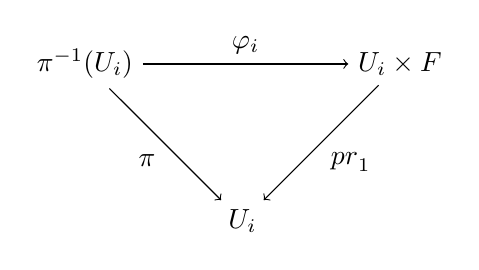
\begin{tikzpicture}
                \node (PI) at (-2, 0) {$\pi^{-1}(U_i)$};
                \node (UF) at (2, 0) {$U_i\times F$};
                \node (U) at (0, -2) {$U_i$};
                \draw[->] (PI) -- node[above]{$\varphi_i$} (UF);
                \draw[->] (PI) -- node[below left]{$\pi$} (U);
                \draw[->] (UF) -- node[below right]{$\text{pr}_1$} (U);
            \end{tikzpicture}
        \end{figure}
        As for general bundles one calls $E$ and $B$ the \textbf{total space} and \textbf{base space} respectively. The space $F$ is called the \textbf{(typical) fibre}. The pair $(U_i,\varphi_i)$ is sometimes called a \textbf{bundle chart} and the set $\{(U_i,\varphi_i)\}_{i\in I}$ is often called a \textbf{local trivialization}\footnote{This name follows from the fact that the bundle is locally isomorphic to a (trivial) product space: $E\cong U\times F$.}. The cover $\{U_i\}_{i\in I}$ itself is called a \textbf{trivializing cover} of the bundle.

        The \textbf{transition maps} $\varphi_j\circ\varphi_i^{-1}:(U_i\cap U_j)\times F\rightarrow (U_i\cap U_j)\times F$ can be identified with the cocycle $g_{ji}:U_i\cap U_j\rightarrow G$, associated to the (left) action (which is required to be faithful\footnote{See definition \ref{group:faithful_action}.}) of $G$ on every fibre, by the following relation:
        \begin{gather}
            \varphi_j\circ\varphi_i^{-1}(b, x) = (b, g_{ji}(b)\cdot x).
        \end{gather}
    }
    \begin{remark}
        One should pay attention to the fact that the bundle charts are not coordinate charts in the sense of manifolds \ref{diff:chart} because the image of $\varphi_i$ is not an open subset of $\mathbb{R}^n$. However, they serve the same purpose as they are used to locally describe the total space $P$.
    \end{remark}
    \begin{notation}
        A fibre bundle $(E,B,\pi,F,G)$ is often denoted by $F\hookrightarrow E\xrightarrow{\ \pi\ }{B}$ or even $\pi:E\rightarrow B$ if the fibre is not important. A drawback of such notations is that the structure group of the bundle is not shown.
    \end{notation}

    \newdef{Numerable fibre bundle}{\index{numerable}\label{diff:numerable_bundle}
        A fibre bundle that admits a local trivialization over a numerable open cover.
    }

    \newdef{Compatible\footnotemark\ bundle charts}{\index{compatible!bundle charts}
        \footnotetext{Also called an \textbf{admissible chart}.}
        A bundle chart $(V,\psi)$ is said to be compatible with a trivializing cover $\{(U_i,\varphi_i)\}_{i\in I}$ if whenever $V\cap U_i\neq\emptyset$, there exists a map $h_i:V\cap U_i\rightarrow G$ such that
        \begin{gather}
            \psi\circ\varphi_i^{-1}(b,x) = (b,h_i(b)x)
        \end{gather}
        for all $b\in V\cap U_i$ and $x\in F$. Two trivializing covers are said to be equivalent if all bundle charts are cross-compatible. As in the case of manifolds, this gives rise to the notion of a \textbf{$G$-atlas}. A \textbf{$G$-bundle} is then defined as a fibre bundle eqipped with an equivalence class of $G$-atlases.
    }

\section{Bundle maps}

    \newdef{Bundle map}{\index{bundle!map}
        A bundle map between two fibre bundles $\pi_1:E_1\rightarrow B_1$ and $\pi_2:E_2\rightarrow B_2$ is a pair $(f_E,f_B)$ of morphisms that make diagram \ref{fig:bundle_map} commute. The map $f_E$ is said to \textbf{cover} $f_B$. If such a couple exists, the base map $f_B$ is uniquely determined by $f_E$ and therefore a bundle map is often just denoted by $f_E:E_1\rightarrow E_2$.

        \begin{figure}[ht!]
        \centering
        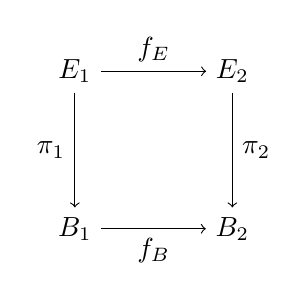
\begin{tikzpicture}
            \node (E1) at (0, 0) {$E_1$};
            \node (E2) at (2, 0) {$E_2$};
            \node (B1) at (0, -2) {$B_1$};
            \node (B2) at (2, -2) {$B_2$};
            \draw[->] (E1) -- node[above]{$f_E$} (E2);
            \draw[->] (E1) -- node[left]{$\pi_1$} (B1);
            \draw[->] (E2) -- node[right]{$\pi_2$} (B2);
            \draw[->] (B1) -- node[below]{$f_B$} (B2);
        \end{tikzpicture}
        \caption{Bundle map between fibre bundles.}
        \label{fig:bundle_map}
        \end{figure}
    }
    \newdef{Isomorphism}{
        Two fibre bundles $F$ and $G$ are said to be isomorphic if there exist bundle maps $f:F\rightarrow G$ and $g:G\rightarrow F$ such that $f\circ g = \mathbbm{1}_G$ and $g\circ f = \mathbbm{1}_F$.
    }

    \newdef{Equivalent fibre bundles}{\index{gauge!transformation}
        Two fibre bundles $\pi_1:E_1\rightarrow B$ and $\pi_2:E_2\rightarrow B$, with the same typical fibre and structure group, are said to be equivalent if there exist trivializations\footnote{Remark that the collection $\{U_i\}_{i\in I}$ is the same for both trivializations.} $\{(U_i,\varphi_i)\}_{i\in I}$ and $\{(U_i,\varphi'_i)\}_{i\in I}$ such that the associated cocycles are equivalent. An explicit form of the functions $\lambda$ is given by
        \begin{gather}
            \lambda_{i,i} := \varphi_i'\circ\varphi_i^{-1}.
        \end{gather}
    }
    \begin{property}
        Two fibre bundles over the same base space are equivalent if and only if they are isomorphic.
    \end{property}

    \newdef{Trivial bundle}{\index{trivial}\label{diff:trivial_bundle}
        A fibre bundle $(E,B,\pi,F)$ is said to be trivial if there exists an equivalence $E\cong B\times F$.
    }

\section{Constructions}

    \begin{construct}[Fibre bundle construction theorem]\label{diff:fibre_bundle_construction_theorem}
        Let $M$ and $F$ be spaces and let $G$ be a group equipped with a left action on $F$. Suppose that a cover $\{U_i\}_{i\in I}$ of $M$ and a collection of morphisms $\{g_{ji}:U_i\cap U_j\rightarrow G\}$ that satisfy the cocycle condition \ref{diff:G_cocycle} are given. A fibre bundle over $M$ can then be constructed as follows:
        \begin{enumerate}
            \item First construct for every set $U_i$ an associated set $U_i\times F$.
            \item Then construct the disjoint union $T:=\bigsqcup_{i\in I}U_i\times F$ and equip it with the disjoint union topology (see definition \ref{topology:disjoint_union}).
            \item From this disjoint union construct a quotient space and equip it with the quotient space topology (see definition \ref{topology:quotient_space}) induced by the following equivalence relation for every $i,j\in I$:
                \begin{gather}
                    (p, f)\sim(p,g_{ji}(x)\cdot f)
                \end{gather}
                for all $x\in U_i\cap U_j$ and $f\in F$.
            \item The fibre bundle is equal to the quotient space $T/\sim$ equipped with the projection $\pi$ that maps the equivalence class $(x,f)\in T$ to $x\in M$.
            \item Local trivializations are given by the maps $\varphi_i:\pi^{-1}(U_i)\rightarrow U_i\times F$ that satisfy
                \begin{gather}
                    \varphi_i^{-1}:(x,f)\mapsto [(x,f)],
                \end{gather}
                where $[A]$ denotes the equivalence class of $A$ in $T/\sim$.
        \end{enumerate}
    \end{construct}
    \begin{property}[Homotopy invariance]
        Homotopic transition functions give rise to equivalent (and hence isomorphic) bundles. (This follows from the homotopy invariance of \v{C}ech cohomology.)
    \end{property}

    \begin{remark}[Clutching]\index{clutching}
        The above construction is often called the clutching construction, especially when constructing vector bundles over a sphere $S^n$. There the covering consists of two hemispheres that intersect on the equator $S^{n-1}$ and the function $g_{21}$ is in that case also called the \textbf{clutching function}.
    \end{remark}
    \begin{property}[Vector bundles over a sphere]\index{vector!bundle}\label{diff:vector_bundles_over_sphere}
        The clutching theorem and the homotopy invariance imply that vector bundles over the sphere are determined by homotopy classes of functions $S^{n-1}\rightarrow\text{GL}_p(k)$, i.e. they are classified by the homotopy group $\pi_{n-1}(\text{GL}_p(k))$.
    \end{property}

    \newdef{Subbundle}{\index{sub!bundle}
        A subbundle of a fibre bundle $\pi:E\rightarrow B$ is a triple $(E',B',\pi')$ such that $E'\subset E$, $B'\subset B$ and $\pi' = \pi|_{E'}$.
    }
    \newdef{Pullback bundle}{\index{pullback!bundle}\label{diff:pullback_bundle}
        Let $\pi:E\rightarrow B$ be a fibre bundle and let $f:B'\rightarrow B$ be a morphism of spaces. The total space of the pullback bundle $f^*E$ is defined as follows:
        \begin{gather}
            f^*E := \big\{(b',e)\in B'\times E:f(b') = \pi(e)\big\}.
        \end{gather}
        The topology on $f^*E$ is induced by the subspace topology of the product $B'\times E$. The projection onto the second factor gives a map of total spaces $f^*E\rightarrow E$.
    }

    \newdef{Fibre product}{\index{fibre!product}
        Let $(F_1,B,\pi_1)$ and $(F_2,B,\pi_2)$  be two fibre bundles over the same base space $B$. Their fibre product is defined as follows:
        \begin{gather}
            \label{diff:fibre_product}
            F_1\diamond F_2 := \big\{(f, g)\in F_1\times F_2: \pi_1(f) = \pi_2(g)\big\}.
        \end{gather}
    }

\section{Sections}

    \newdef{Section}{\index{section}
        A (\textbf{global}) section of a fibre bundle $\pi:E\rightarrow B$ is a morphism $s:B\rightarrow E$ such that $\pi\circ s = \mathbbm{1}_B$. For any open subset $U\subset B$ a \textbf{local} section is defined as a morphism $s_U:U\rightarrow E$ such that $\pi\circ s_U(b) = b$ for all $b\in U$.
    }
    \begin{notation}
        \nomenclature[O_Gamma]{$\Gamma(E)$}{set of global sections of a fibre bundle $E$}
        The set of all global sections of a bundle $E$ is denoted by $\Gamma(E)$. The set of local sections over $U$ is sometimes denoted by $\Gamma(U, E)$. With this latter notation one also has $\Gamma(E)\equiv\Gamma(B, E)$.
    \end{notation}

    \begin{property}[Pullback of sections]
        The sections of a fibre bundle $E$ pullback to the pullback bundle $f^*E$ by setting $f^*s := s\circ f$.
    \end{property}
\section{Connections}
\subsection{Vertical bundle}
	
	Because smooth fibre bundles (which include smooth principal G-bundles) are also smooth manifolds we can define the traditional notions for them, such as the tangent bundle. We use this to construct the notions of horizontal and vertical bundles:
	\newdef{Vertical vector}{\index{vertical vector}
		Let $\pi:E\rightarrow B$ be a smooth fibre bundle. The subbundle $\ker(T\pi)$ of $TE$ is called the vertical bundle of $E$. Fibrewise this gives us $V_x = T_x(E_{\pi(x)})$.
	}

	For principal G-bundles we can use an equivalent definition:
	\begin{adefinition}
		Consider a smooth principal $G$-bundle $G\hookrightarrow P\xrightarrow{\pi} M$. We first construct a map $\iota_p$ for every element $p\in P$:
		\begin{equation}
			\iota_p:G\rightarrow P: g\mapsto p\cdot g
		\end{equation}
		We then define a tangent vector $v\in T_p P$ to be vertical if it lies in the image of $T_e\iota_p$, i.e. $\text{Vert}(T_pP) = \text{im}(T_e\iota_p)$. This construction is supported by the exactness of following short sequence:
		\begin{equation}
			0\xrightarrow{} \mathfrak{g} \xrightarrow{T_e\iota_p} T_p P\xrightarrow{T_p\pi} T_xM \xrightarrow{} 0
		\end{equation}
	\end{adefinition}
	\begin{property}[Dimension]
		It follows from the second definition that the vertical vectors of a principal G-bundle are nothing but the pushforward of the Lie algebra $\mathfrak{g}$ under the right action of $G$ on $P$. Furthermore, the exactness of the sequence implies that $T_e\iota_p:\mathfrak{g}\rightarrow\text{Vert}(T_pP)$ is an isomorphism of vector spaces. In particular, it implies that
		\begin{equation}
			\label{manifolds:vertical_dimension}
			\dim\text{Vert}(T_pP) = \dim\mathfrak{g} = \dim G
		\end{equation}
	\end{property}
	
	\newdef{Fundamental vector field}{
		Consider a principle $G$-bundle. Let $A\in\mathfrak{g}$, where $\mathfrak{g}$ is the Lie algebra corresponding to $G$. The vertical vector field $A^\#:P\rightarrow TP$ given by
		\begin{equation}
			\label{manifolds:fundamental_vector_field}
			A^\#(p) = \iota_{p,\ast}(A)\in\text{Vert}(T_pP)
		\end{equation}
		is called the fundamental vector field associated to $A$.
	}
	\begin{property}
		The map $(\cdot)^\#:\mathfrak{g}\rightarrow\Gamma(TP)$ is a Lie algebra morphism:
		\begin{equation}
			[A, B]^\# = [A^\#, B^\#]
		\end{equation}
		where the Lie bracket on the left is that in $\mathfrak{g}$ and the Lie bracket on the right is that in $\mathfrak{X}(M)$ given by \ref{manifolds:lie_bracket}.
	\end{property}
	
		\begin{property}
		The vertical bundle satisfies the following $G$-equivariance condition:
		\begin{equation}
			R_{g, \ast}(\text{Vert}(T_pP)) = \text{Vert}(T_{pg}P)
		\end{equation}
		
		By differentiating the equality \[R_g\circ\iota_p = \iota_{pg}\circ\text{ad}_{g^{-1}}\] and using \ref{manifolds:fundamental_vector_field} and \ref{lie:adjoint_rep_of_group} we obtain the following algebraic formulation of the $G$-equivariance condition:
		\begin{equation}
			R_{g, \ast}\left(A^\#(p)\right) = \left(\text{Ad}_{g^{-1}}A\right)^\#(pg)
		\end{equation}
	\end{property}
	
\subsection{Horizontal bundle}

	\newdef{Connection}{\index{connection}
		\label{manifolds:connection}
		Consider a principal bundle $P$ with structure group $G$. A connection on $P$ is the selection of a subspace $\text{Hor}(T_pP)\leq T_pP$ for every $p\in P$ such that:
		\begin{itemize}
			\item $\text{Vert}(T_pP)\oplus\text{Hor}(T_pP) = T_pP$
			\item The selection depends smoothly on $p$.\footnote{See the definiton of a (smooth) distribution \ref{manifolds:distribution}.}
			\item The subspace $\text{Hor}(T_pP)$ is $G$-equivariant:
			\begin{equation}
				R_{g, \ast}(\text{Hor}(T_pP)) = \text{Hor}(T_{pg}P)
			\end{equation}
		\end{itemize}
		The elements of $\text{Hor}(T_pP)$ are said to be \textbf{horizontal vectors} with respect to the connection.
	}
	\begin{remark}
		Remark that the $G$-invariance condition for vertical bundles is an intrinsic property while we have to require it by definition for the horizontal bundle.
	\end{remark}
	
	\newdef{Horizontal bundle}{
		The horizontal bundle $\text{Hor}(TP)$ is defined as $\bigcup_{p\in P}\text{Hor}(T_pP)$. It is a subbundle of $TP$. The $G$-invariance condition then implies that this subbundle is invariant under (the pushforward of) the  right action of $G$.
	}
	
	\begin{property}[Dimension]
		Properties \ref{manifolds:principal_bundle_dimension}, \ref{manifolds:vertical_dimension} and the direct sum decomposition of $T_pP$ imply the following relation:
		\begin{equation}
			\dim\text{Hor}(T_pP) = \dim M
		\end{equation}
	\end{property}
	\begin{property}
		\label{manifolds:connection_dimensions}
		We take some time to summarize all dimensional relations between the components of a principal $G$-bundle over a base manifold $M$:
		\begin{empheq}[box=\widefbox]{align}
			\dim P &= \dim M + \dim G\\
			\dim M &= \dim\text{Hor}(T_pP)\\
			\dim G &= \dim\text{Vert}(T_pP)
		\end{empheq}
		for all $p\in P$.
	\end{property}
	
	\newdef{Dual connection}{\index{dual!connection}
		First we define the dual of the horizontal bundle:
		\begin{equation}
			\text{Hor}(T_p^*P) = \{h^*\in T_p^*P|h^*(v)=0, v\in\text{Vert}(T_pP)\}
		\end{equation}
		Equivalently, the horizontal covector bundle is defined as the set of linear functionals that annihilate vertical vectors. Just as with the vertical bundle this structure is independent of any connection on $P$.
		
		A dual connection can then be defined as the selection of a vertical covector bundle $\text{Vert}(T_p^*P)$ satisfying the conditions of definition \ref{manifolds:connection} where $\text{Vert}$ and $\text{Hor}$ should be interchanged.
	}
	
\subsection{Ehresmann connection}\index{Ehresmann connection}

	\newdef{Ehresmann connection}{
		Let $(P, M, \pi, G)$ be a principal bundle. An Ehresmann connection is a $\mathfrak{g}$-valued 1-form $\omega:TP\rightarrow\mathfrak{g}$ that satisfies following 2 conditions:
		
		\begin{enumerate}
			\item
			\begin{equation}
				\omega\circ R_{g, \ast} = \text{Ad}_{g^{-1}}\circ\omega
			\end{equation}
			\item
			\begin{equation}
				\omega(A^\#) = A
			\end{equation}
		\end{enumerate}
		The horizontal subspaces are then defined as $\text{Hor}(T_pP) = \ker\omega|_p$.
	}
	
	\begin{property}
		Consider two principal $G$-bundles $\xi_1$ and $\xi_2$. Let $\omega$ be an Ehresmann connection on $\xi_1$ and let $F;\xi_1\rightarrow \xi_2$ be a bundle map covering a smooth map $f$. The map $F^*\omega$ defines an Ehresmann connection on $\xi_2$.
	\end{property}
	
	\begin{example}
		Consider a principal $G$-bundle. An Ehresmann connection on this bundle is given by the following map:
		\begin{equation}
			\omega = (T_e\iota_p)^{-1}\circ\pr_V
		\end{equation}
		where $\pr_V$ is the projection $TP\rightarrow\text{Vert}(TP)$ associated to the decomposition from definition \ref{manifolds:connection}.
	\end{example}
	
	\newdef{Horizontal and vertical forms}{\index{horizontal!form}\index{vertical!form}\label{forms:horizontal_form}
		Let $\omega$ be an Ehresmann connection on a principal bundle $\prin{G}{P}{M}$. Let $\theta\in\Omega^k(P)$ be a $k$-form. We define following notions:
		\begin{itemize}
			\item $\theta$ is said to be horizontal if
			\begin{equation}
				\theta(v_1, ..., v_k) = 0
			\end{equation}
			whenever at least 1 of the $v_i$ lies in $\text{Vert}(T_pP)$.
			\item $\theta$ is said to be vertical if
			\begin{equation}
				\theta(v_1, ..., v_k) = 0
			\end{equation}
			whenever at least 1 of the $v_i$ lies in $\text{Hor}(T_pP)$.
		\end{itemize}
		For functions $f\in\Omega^0(P)$ it is vacuously true that they are both vertical and horizontal.
	}
	
\subsection{Maurer-Cartan form}

	\newdef{Maurer-Cartan form}{\index{Maurer-Cartan form}\index{Cartan!(connection) form|see{Maurer-Cartan}}
		For every $g\in G$ we have that the tangent space $T_gG$ is isomorphic to $T_eG\cong\mathfrak{g}$. The isomorphism $T_gG\rightarrow\mathfrak{g}$ is given by the Maurer-Cartan form:
		\begin{equation}
			\boxed{\Omega := L_{g^{-1},\ast}}
		\end{equation}
	}
	
	\begin{definition}
		Consider a manifold $M = \{x\}$. When constructing a principal $G$-bundle over $M$ we see that the total space $P = \{x\}\times G$ can be identified with the structure group $G$. From the relations in property \ref{manifolds:connection_dimensions} we see that the horizontal spaces are null-spaces (which defines a smooth distribution and thus a connection according to \ref{manifolds:connection}) and that the vertical spaces are equal to the tangent spaces, i.e. $\text{Vert}(T_gG) = T_gG$ (where we already made the association $P\cong G$).
		
		The simplest way to define a connection form $\omega$ on this bundle would be the trivial projection $TP\rightarrow\text{Vert}(TP) = \mathbbm{1}_{TP}$. The image of this map would however be $T_gG$ and not $\mathfrak{g}$ as required. This can be solved by using the Maurer-Cartan form $\Omega:T_gG\rightarrow\mathfrak{g}$, i.e. we define $\omega(v) = \Omega(v)$.
	\end{definition}
	
	\begin{property}
		The Maurer-Cartan form is the unique Ehresmann connection on the bundle $G\hookrightarrow G\rightarrow \{x\}$.
	\end{property}
	
\subsection{Horizontal lifts and parallel transport}
	
	\begin{property}\index{horizontal!lift}
		Consider a principal $G$-bundle $G\hookrightarrow P\rightarrow M$ and a curve $\gamma:[0, 1]\rightarrow M$. Let $p_0\in \pi^{-1}(\gamma(0))$. There exists a unique curve $\widetilde{\gamma}_{p_0}:[0, 1]\rightarrow P$ satisfying the following conditions:
		\begin{itemize}
			\item $\widetilde{\gamma}_{p_0}(0) = p_0$
			\item $\pi\circ\widetilde{\gamma}_{p_0} = \gamma$
			\item $\widetilde{\gamma}_{p_0}'(t)\in\text{Hor}(TP)$ for all $t\in[0, 1]$
		\end{itemize}
		The curve $\widetilde{\gamma}_{p_0}$ is said to be the horizontal lift of $\gamma$ starting at $p_0$. When it is clear from the context what the basepoint $p_0$ is, the subscript is often ommited and we write $\widetilde{\gamma}$ instead of $\widetilde{\gamma}_{p_0}$.
	\end{property}
	\begin{remark}[Horizontal curve]\index{horizontal!curve}
		Curves satisfying the last condition are said to be horizontal.
	\end{remark}
	
	\newdef{Parallel transport on principal bundles}{\index{parallel transport!on principal bundles}
		\nomenclature[O]{$\text{Par}_t^\gamma$}{Parallel transport map with respect to the curve $\gamma$.}
		The parallel transport map with respect to the curve $\gamma$ is defined as follows:
		\begin{equation}
			\text{Par}_t^\gamma:\pi^{-1}(\gamma(0))\rightarrow\pi^{-1}(\gamma(t)):p_0\mapsto \widetilde{\gamma}_{p_0}(t)
		\end{equation}
		This map is $G$-equivariant and it is a diffeomorphism of fibres.
	}
	
	\begin{formula}
		Consider a principal bundle $G\hookrightarrow P\rightarrow M$. Let $\gamma(t)$ be a curve in $M$ and let $\omega$ be an Ehresmann connection on this bundle. The horizontal lift of $\gamma(t)$ can locally be parametrized as $(\gamma(t), g(t))$ where $g(t)$ is some unique curve in $G$. To determine $\widetilde{\gamma}(t)$ it is thus sufficient to find $g(t)$. The following parametrization uniquely characterizes $g(t)$:
		\begin{equation}
			g'(t) = -\omega(\gamma(t), \mathbbm{1}_G, \gamma'(t), 0)g(t)
		\end{equation}
		Using the trivial section $s:U\rightarrow U\times G:x\mapsto (x, \mathbbm{1}_G)$ where $U$ is an open subset of $M$ we can rewrite this formula as follows: First we consider the action of the pullback $s^*\omega$ on the derivative $\gamma_*: \mathbb{R}\times\mathbb{R}\rightarrow TM:(t, 1) \mapsto (\gamma(t), \gamma'(t))$. Using the fact that it is linear in the second argument we can write\[s^*\omega(\gamma(t), \gamma'(t)) = A(\gamma(t))\gamma'(t)\]where $A:M\rightarrow\text{Hom}(\mathbb{R}^{\dim M}, \mathfrak{g})$ gives a linear map for each point $\gamma(t)\in M$. The action can also be rewritten using the relation $f^*\omega = \omega\circ f_\ast$ as\[s^*\omega(\gamma(t), \gamma'(t)) = \omega\Big(s_\ast(\gamma(t), \gamma'(t))\Big) = \omega(\gamma(t), \mathbbm{1}_G, \gamma'(t), 0)\]
		Combining these relations with the ODE for $g(t)$ gives
		\begin{equation}
			\left(\deriv{}{t} + A(\gamma(t))\gamma'(t)\right)g(t) = 0
		\end{equation}
		where $\deriv{}{t}$ is a matrix given by the scalar multiplication of the derivative $\deriv{}{t}$ and the unit matrix $I$.
	\end{formula}
	
	\newdef{Holonomy group}{\index{holonomy}
		\nomenclature[S]{$\text{Hol}_p(\omega)$}{Holonomy group at $p$ with respect to the connection $\omega$.}
		Consider a principal bundle $\prin{G}{P}{M}$. Let $\Omega^{ps}_mM\subset\Omega M$ be the loop space with basepoint $m\in M$ of piecewise smooth loops. The holonomy group $\text{Hol}_p(\omega)$ based at $p\in\pi^{-1}(m)\subset P$ with respect to the connection form $\omega$ is given by:
		\begin{equation}
			\text{Hol}_p(\omega) = \{g\in G: p \text{ and } p\cdot g \text{ can be connected by a $\widetilde\gamma$}, \gamma\in\Omega^{ps}_mM\}
		\end{equation}
	}
	\newdef{Reduced holoomy group}{
		The reduced holonomy group $\text{Hol}_p^0(\omega)$ is defined as the subset of $\text{Hol}_p(\omega)$ using only contractible loops.
	}
	
\subsection{Koszul connections and covariant derivatives}

	\newdef{Parallel transport on vector bundles}{
		Consider a principal bundle $G\hookrightarrow P\rightarrow M$ where we explicitly require $P$ to be trivial, i.e. $P = M\times G$. Suppose that the Lie group $G$ acts on a vector space $V$ by a representation $\rho:G\rightarrow GL_m$ . We can then construct an associated vector bundle $\pi_1:M\times V\rightarrow M$.
		
		Parallel transport on this vector bundle is then defined as follows. Let $\gamma(t)$ be a curve in $M$ such that $\gamma(0)=x_0$ and $x_1 = \gamma(1)$. Furthemore, let the horizontal lift $\widetilde{\gamma}(t)$ have $\widetilde{\gamma}(0)=(x_0, h)$ as initial condition. The parallel transport of the point $(x_0, v_0)\in M\times V$ along $\gamma$ is given by the following map:
		\begin{equation}
			\text{Par}^\gamma_t:\pi^{-1}_1(x_0)\rightarrow\pi^{-1}_1(\gamma(t)):(x_0, v_0)\mapsto \big(\gamma(t), \rho\big(g(t)h^{-1}\big)v_0\big)
		\end{equation}
		It should be noted that this map is independent of the initial element $h\in G$. Furthermore, $\text{Par}^\gamma_t$ is an isomorphism of vector spaces and can thus be used to identify distant fibers (as long as they lie in the same path-component).
	}
	\begin{remark}
		Two remarks have to be made. First of all, although the previous construction explicitly used trivial bundles, it is also valid for general non-trivial vector bundles. Secondly, following remark \ref{manifolds:vector_principal_correspondence} we can construct a principal bundle for any vector bundle and use the parallel transport on this bundle to define parallel transport of vectors. The previous construction is thus possible for every vector bundle.
	\end{remark}
	
	\newdef{Covariant derivative}{\index{covariant!derivative}
		Consider a vector bundle with model fibre space $V$ and its associated principal $GL(V)$-bundle with Ehresmann connection $\omega$, both over a base manifold $M$. Let $\sigma:M\rightarrow E$ be a section of the vector bundle and let $X$ be a vector field on $M$. The covariant derivative of $\sigma$ with respect to $X$ is defined as:
		\begin{equation}
			\nabla_X\sigma(x_0) = \lim_{t\rightarrow+\infty}\stylefrac{(\text{Par}_t^\gamma)^{-1}\sigma(\gamma(t)) - \sigma(x_0)}{t}
		\end{equation}
		where $\gamma(t)$ is any curve such that $\gamma(0) = x_0$ and $\gamma'(0) = X(x_0)$.
	}
	\begin{property}
		Let $\pi:E\rightarrow M$ be a vector bundle. Let $\sigma, X$ and $f$ be respectively a section on $E$, a vector field on $M$ and a $C^\infty$ function on $M$. The covariant derivative along $X$ satisfies following properties:
		\begin{itemize}
			\item $\nabla_X\sigma$ is a smooth section on $E$.
			\item The map $(X, \sigma)\mapsto\nabla_X\sigma$ is bilinear over $\mathbb{R}$.
			\item $\nabla_{(fX)}\sigma = f\nabla_X\sigma$
			\item $\nabla_X(f\sigma) = f\nabla_X\sigma + X(f)\sigma$
		\end{itemize}
	\end{property}
	\begin{remark}
		The last two properties show the major difference between the Lie derivative and the covariant derivative when $\sigma$ is a section of the tangent bundle, i.e. a vector field. Lie derivatives depend on the local behaviour of both $X$ and $\sigma$. The covariant derivative on the other hand only depends on the value of $X$ at $p\in M$ and on the local behaviour of $\sigma$.
	\end{remark}
	
	\newdef{Koszul connection}{\index{Koszul!connection}
		The map
		\begin{equation}
			\Gamma(TM)\times\Gamma(E)\rightarrow\Gamma(E):(X, \sigma)\mapsto\nabla_X\sigma
		\end{equation}
		is called a Koszul connection if the above properties hold. From the above constructions it also follows that every Ehresmann connection on a principal bundle induces a Koszul connection on all of its associated vector bundles.
	}
	
	\newdef{Exterior covariant derivative}{\index{exterior!covariant derivative}
		Consider a principal bundle $\prin{G}{P}{M}$ equipped with an Ehresmann connection $\omega$. Let $\theta\in \Omega^k(P)$ be a differential $k$-form. The exterior covariant derivative $D\theta$ is defined as follows:
		\begin{equation}
			D\theta(v_0, ..., v_k) = d\theta(v_0^H, ..., v_k^H)
		\end{equation}
		where $d$ is the exterior derivative \ref{forms:def:exterior_derivative} and $v_i^H$ is the projection of $v_i$ on the horizontal subspace $\text{Hor}(T_pP)$ associated to the Ehresmann connection $\omega$. From the definition it follows that the covariant derivative $D\theta$ is a horizontal form \ref{forms:horizontal_form}.
	}
	\begin{remark}
		The exterior covariant derivative can also be defined for general $W$-valued $k$-forms where $W$ is a vector space. This can be done by defining it component-wise with respect to a given basis on $W$. Afterwards one can prove that the choice of basis plays no role.
	\end{remark}
	
	\begin{formula}
		Using the Koszul connection on the tangent bundle $TP$ we can rewrite the action of the exterior covariant derivative as follows:
		\begin{equation}
			D\theta(v_0, ..., v_k) = \sum_i^k(-1)^i\nabla_{v_i}\theta(v_0, ..., \hat{v}_i, ..., v_k) + \sum_{i<j}^k(-1)^{i+j}\theta([v_i, v_j], v_0, ..., \hat{v}_i, ..., \hat{v}_j, ..., v_k)
		\end{equation}
		where $\hat{v}_i$ means that this vector is omitted. As an example we explicitly give the formula for a 1-form $\Phi$:
		\begin{equation}
			D\Phi(X, Y) = \nabla_X(\Phi(Y)) - \nabla_Y(\Phi(X)) - \Phi([X, Y])
		\end{equation}
		which should remind the reader of the analogous formula for the ordinary exterior derivative \ref{forms:k_form_exterior_derivative}.
	\end{formula}
	
\subsection{Curvature of a connection}

	\newdef{Curvature}{\index{curvature}
		Let $\omega$ be an Ehresmann connection on a principal bundle $\prin{G}{P}{M}$. The curvature of $\omega$ is defined as the exterior covariant derivative $D\omega$.
	}
	\newdef{Flat connection}{
		An Ehresmann connection $\omega$ is said to be flat if its curvature $D\omega$ vanishes everywhere.
	}
	
	The following property is an immediate consequence of the Frobenius integrability theorem \ref{manifolds:frobenius} and the fact that an Ehresmann connection vanishes on the horizontal subbundle.
	\begin{property}\index{integrable}
		Let $\omega$ be an Ehresmann connection. The associated horizontal distribution\footnote{See \ref{manifolds:distribution} for the definition of a distribution of vector spaces.}\[p\mapsto\text{Hor}(T_pP)\]is integrable if and only if the connection $\omega$ is flat. The vertical distribution is always integrable.
	\end{property}

\section{Integration Theory}\label{section:integration_manifolds}

    For the theory on measure spaces and Lebesgue integration see chapter \ref{chapter:lebesgue}.

\subsection{Orientation and densities}

    One can define an orientation of manifolds by generalizing the situation for vector spaces \ref{tensor:orientation}:
    \newdef{Orientable manifold}{\index{orientation}\index{volume}\label{diff:orientability}
        First, we slightly modify the definition of the volume element. A \textbf{volume form} on $M$ is a nowhere-vanishing top-dimensional differential form $\text{Vol}\in\Omega^n(M)$ where $n=\dim(M)$. The definition of an orientation is then virtually the same as for vector spaces.

        An \textbf{oriented atlas} is given by all charts of $M$ for which the pullback of the Euclidean volume form is a positive multiple of $\text{Vol}$. This also implies that the transition functions have a positive Jacobian determinant. The existence of such a volume form turns a differentiable manifold into an \textbf{orientable manifold}.

        Alternatively, an orientable manifold with volume form $\text{Vol}$ is said to be \textbf{positively oriented} if it comes equipped with a smooth choice of bases $\{v_1,\ldots,v_n\}$ for $T_pM$ such that $\text{Vol}(v_1,\ldots,v_n)>0$.
    }

    \begin{example}\index{determinant}
        Let $M=\mathbb{R}^n$. The canonical Euclidean volume form is given by the determinant map
        \begin{gather}
            \det:(u_1,\ldots,u_n)\mapsto\det(u_1,\ldots,u_n)
        \end{gather}
        where the $u_n$'s are expressed in the canonical basis $(e_1,\ldots,e_n)$. The terminology of ''volume forms'' is justified by noting that the determinant map gives the signed volume of the $n$-dimensional parallelotope spanned by the vectors $\{u_1,\ldots,u_n\}$.
    \end{example}

    \begin{property}
        Let $\omega_1,\omega_2$ be two volume forms on $M$. There exists a smooth function $f$ such that \[\omega_1 = f\omega_2.\] Furthermore, the sign of this function is constant on every connected component of $M$.
    \end{property}

    One can also rephrase orientability of manifolds in terms of bundles:
    \newdef{Orientation bundle}{\index{orientation}
        Consider a smooth manifold $M$ with its tangent bundle $TM$. The transition function $A$ of $TM$ is given by the Jacobian of the transitions functions on $M$. The associated line bundle with transition function $\sgn\det(A)$ is called the orientation bundle $o(M)$.

        In general one can define the orientation bundle $o(E)$ for any vector bundle $E$, where one replaces the Jacobian in the above construction by the transition maps of $E$. From this it is clear that the orientation bundle $o(M)$ is the same as $o(TM)$.
    }
    \newadef{Orientable manifold}{
        A smooth manifold is orientable if its orientation bundle is trivial.
    }
    \begin{property}[Orientability]
        A smooth manifold is orientable if and only if its canonical line bundle \ref{diff:canonical_bundle} is trivial. Furthermore, for orientable manifolds there exists an isomorphism $\Gamma(\det(T^*M))\cong\Gamma(|\Omega|(M))$.
    \end{property}

    \begin{remark}
        By definition of the orientation bundle, the transition functions are those that have a positive determinant. This gives the equivalence with definition \ref{diff:orientability}. In the next chapter on principal bundles we will give yet another (equivalent) definition of orientability in terms of $G$-structures (see example \ref{diff:orientable_structure}).
    \end{remark}

    In a later paragraph in this section we will generalize integration from orientable manifolds to non-orientable manifolds. To achieve this goal we will need to generalize the notion of differential forms. A good introduction for this is \cite{tensor_bundle_calculus}.
    \newdef{Pseudoscalars}{\index{pseudo!scalar}
        Consider a group morphism $\phi:G\rightarrow\text{O}(p, q)$ for some $p,q\in\mathbb{N}$. The pseudoscalar representation of $G$, induced by $\phi$, is defined as the one-dimensional representation given by
        \begin{gather}
            \mathbf{1}_\sgn:g\mapsto\det(\phi(g)).
        \end{gather}
        The notation $\mathbf{1}_\sgn$ refers to the fact that this representation is a generalization of the \textit{alternating (or sign) representation} of the permutation groups $S_n$.

        Sections of vector bundle with defined by $\mathbf{1}_\sgn$ are generally called \textbf{pseudoscalar fields}.  When twitsing a vector bundle by the pseudoscalar bundle $\Psi$ over $M$, we often add the prefix ''pseudo'' to the name of the bundle $E$, e.g. the $\Psi$-twisted $k$-form bundle is called the bundle of $k$-pseudoforms.

        Any Riemannian manifold admits a canonical pseudoscalar bundle $\Psi$ associated to its (orthogonal) frame bundle. In fact for such manifolds the pseudoscalar bundle coincides with the following slightly different construction:
    }

    \begin{definition}[Tensor density]\index{tensor!density}\label{diff:density}
        Consider a vector bundle $E\rightarrow M$ defined by transition maps $A$. The associated bundle of (tensor) $s$-densities is obtained by using the representation
        \begin{gather}
            \rho:A\mapsto\det(A)^{-s}
        \end{gather}
        The number $s$ is called the \textbf{weight} of the density. For $E\equiv TM$ one obtains the (tensor) $s$-densities on $M$, which in the case of $s=1$ are equivalent to top-dimensional forms on $M$. When twisting a vector bundle by an $s$-density bundle, the prefix ''$s$-weighted'' is often added.
    \end{definition}

    \begin{example}[Pseudovectors]\index{pseudo!vector}
        If we consider the representation
        \begin{gather}
            \rho:A\mapsto\sgn\det(A)A,
        \end{gather}
        we can construct a bundle similar to the tangent bundle where the sign of the cocycles $t_{ji}$ now has an influence on the fibres. Sections of such bundles are called \textbf{pseudovector fields}. This construction is equivalent to twisting the tangent bundle by the pseudoscalar bundle $\Psi$, hence its name.
    \end{example}

    \begin{remark}[Honest densities]\index{density}
        Now one should pay incredible attention to the definition of a \textbf{density} (i.e. without the prefix ''tensor''). A density is defined as an $n$-pseudoform, i.e. a section of the \textbf{density bundle} $|\Omega|(M):=\Omega^n(M)\otimes o(M)$. Hence the transition function is $|\det(A)|$, where $A$ is the transition function of $T^*M$.\footnote{One can also define honest $s$-densities $|\Omega|^s(M)$ by combining definition \ref{diff:density} with the orientation bundle to obtain transition maps $|\det(A)|^s$ (for $A$ the cotangent transition map). This is also the only possible way to generalize the $s$-densities of definition \ref{diff:density} to real $s$.}  These are the objects one can integrate over any manifold, even the non-orientable ones. They are essentially maps $\Gamma(\det(T^*M))\rightarrow C^\infty(M)$.

        A naive way to construct a density on a manifold $M$ is by choosing a volume form $\text{Vol}$ and taking the absolute value $|\text{Vol}|$.
    \end{remark}

\subsection{Integration of top-dimensional forms}\index{Lebesgue!integral}\index{measure}

    \newdef{Measure zero}{\index{null!set}
        A subset $U\subset M$ of an orientable manifold is said to be of measure zero if it is the countable union of inverse images (with respect to the chart maps on $M$) of null sets in $\mathbb{R}^n$.
    }

    \newdef{Integrable form}{
        A differential form is said to be integrable if its components with respect to any basis of $\Omega^k(M)$ are Lebesgue integrable on $\mathbb{R}^n$.
    }

    \begin{formula}[Integration of compactly supported forms]
        Consider a form $\omega\in\Omega^{\dim(M)}$ on $M$ with compact support on a coordinate patch $U\subset M$.
        \begin{gather}
            \label{forms:integration_compact_support}
            \int_M\omega = \int_U\omega := \int_{-\infty}^{+\infty}\cdots\int_{-\infty}^{+\infty}\omega_{12\ldots n}(x)dx^1dx^2\cdots dx^n.
        \end{gather}
        This integral is well-defined because under an orientation-preserving change of coordinates the component $\omega_{1\ldots n}$ transforms as $\omega'_{1\ldots n} = \det(J)\omega_{1\ldots n}$ where $J$ is the Jacobian of the coordinate transformation. Inserting this in the integral and replacing $dx_i$ by $dx'_i$ then gives us the well-known change-of-variables formula from Lebesgue integration theory.

        If we require the manifold $M$ to be paracompact, such that to every open cover $\{U_i\subseteq M\}_{i\in I}$ there is associated a subordinate partition of unity $\{\phi_i\}_{i\in I}$, we define the integral of a general compactly supported form $\omega\in\Omega^n(M)$ as follows:
        \begin{gather}
            \int_M\omega := \sum_{i\in I}\int_{U_i}\rho_i\omega.
        \end{gather}
    \end{formula}
    \begin{remark}
        Although we only defined integration for compactly supported forms, the general formula can also sometimes be applied to general forms. It is well-defined whenever the forms $\rho_i\omega$ are integrable and the sum in the definition converges.
    \end{remark}

    \newprop{Compact manifolds}{
        Let $M$ be a smooth compact manifold. Because every form on $M$ is obviously compactly supported, all forms are integrable on $M$.
    }

    \newprop{Invariance under pullbacks}{
        Consider an orientation-preserving diffeomorphism $f:M\rightarrow N$.
        \begin{gather}
            \int_Mf^*\omega = \int_N\omega
        \end{gather}
    }

    \begin{notation}
        Because the integral of differential forms satisfies properties similar to the ones listed in \ref{lebesgue:general_properties}, we introduce the following notation:
        \begin{gather}
            \langle M, \omega \rangle := \int_M\omega.
        \end{gather}
    \end{notation}

\subsection{Stokes's theorem}

    \begin{theorem}[Stokes's theorem]\index{Stokes!theorem for differential forms}
        \label{forms:theorem:stokes_theorem}
        Let $M$ be an orientable smooth manifold with boundary $\partial M$ and let $\omega$ be a differential $k$-form on $M$.
        \begin{gather}
            \int_{\partial M}\omega = \int_M d\omega.
        \end{gather}
    \end{theorem}
    \begin{result}
        The Kelvin-Stokes theorem \ref{vectorcalculus:stokes_theorem}, the divergence theorem \ref{vectorcalculus:divergence_theorem} and Green's identity \ref{vectorcalculus:green_indentity} are immediate results of this (generalized) Stokes's theorem.
    \end{result}

\subsection{Distributions}

    For more information on the theory of distributions on Euclidean space, see chapter \ref{chapter:distributions}.

    There are two ways to introduce distributions on general manifolds. Either we use the locally Euclidean character and define distributions on charts and glue them using the right compatibility data (see for example \cite{AMP1}) or we define them as the dual of the space of smooth functions (with compact support) as in the Euclidean case. In this section we follow the second approach.

    We will require our base manifold $M$ to be paracompact and second-countable. Moreover, we will also assume that we are given a Riemannian metric $g$ (see chapter \ref{chapter:riemann} for more information). This data allows us to turn the space of smooth sections of any tensor bundle over $M$ into a Fr\'echet space using a generalization of the seminorms \ref{distribution:D_seminorm} where we replace the (partial) derivatives $\partial^i$ by covariant derivatives $\nabla^i$ ($\nabla$ is the Levi-Civita connection induced by $g$). The norm will now also be the one induced (fibrewise) by $g$. In a similar way we can for every compact subset $K\subset M$ define the space $\mathcal{D}(K, \otimes^p)$ of smooth $p$-tensor fields with support in $K$ and by taking the direct limit (with its associated topology) we obtain the space of smooth compactly supported $p$-tensor fields $\mathcal{D}(M, \otimes^p)$.

    \newdef{Tensor distribution}{\index{distribution!tensor}
        The space of tensor distributions (of order $p$) is defined as the continuous dual of $\mathcal{D}(M, \otimes^p)$.
    }

    Much of the theory of distributions on Euclidean space can be generalized to smooth manifolds without too much trouble (for example we again obtain a dense inclusion $\mathcal{D}\hookrightarrow\mathcal{D}'$). An interesting generalization is the definition of the covariant derivative:
    \newdef{Covariant derivative}{\index{covariant!derivative}
        Let $(M, g)$ be a Riemannian manifold with associated Levi-Civita connection $\nabla$. The covariant derivative of a tensor distribution $T$ is defined using duality as follows (as in the case of Euclidean space this can be interpreted as an extension of the integration by parts formula):
        \begin{gather}
            \langle \nabla T, \sigma\rangle := -\langle T, g\cdot\nabla\sigma\rangle
        \end{gather}
        where $g\cdot\nabla\sigma$ denotes the internal contraction (generalizing the divergence of a vector field) which, in local coordinates, is given by
        \begin{gather}
            (g\cdot\nabla\sigma)^{i_1\ldots i_p} = \nabla_j\sigma^{ji_1\ldots i_p}.
        \end{gather}
    }

    ?? COMPLETE? ??
\chapter{Riemannian Geometry}

\section{Riemannian manifolds}
\subsection{Metric}

	\begin{definition}[Bundle metric]\index{metric!bundle}
		Consider the bundle of second order covariant vectors. Following from \ref{tensor:tensor_product} every section $g$ of this bundle gives a bilinear map \[g_x:T_xM\times T_xM\rightarrow\mathbb{R}\]
		for all $x\in M$. If this map is symmetric and non-degenerate and if it depends smoothly on $p$ it is called a \textbf{(Lorentzian}) metric.\footnote{See also the section about Hermitian forms and metric forms \ref{linalgebra:innerproduct}.}
		
		The maps $\{g_x\}_{x\in M}$ can be `glued' together to form a global metric $g$, defined on the fibre product\footnotemark\ $TM\diamond TM$. Defining this map on $TM\times TM$ is not possible as tangent vectors belonging to different points in $M$ cannot be `compared'. The collection $\{\langle\cdot|\cdot\rangle_x|x\in M\}$ is called a \textbf{bundle metric}\index{metric!bundle}.
		\footnotetext{See definition \ref{manifolds:fibre_product}.}
	\end{definition}

	A Riemannian metric also induces a duality between $TM$ and $T^*M$. This is given by the \textit{flat} and \textit{sharp} isomorphisms:
	\newdef{Musical isomorphisms}{\index{musical isomorphism}\label{riemann:musical_isomorphisms}
		Let $g:TM\times TM\rightarrow\mathbb{R}$ be the Riemannian metric on $M$. The \textbf{flat} isomorphism is defined as:
		\begin{equation}
			\label{manifolds:flat_map}
			\flat:v\mapsto g(v, \cdot)
		\end{equation}
		The \textbf{sharp} isomorphism is defined as the inverse map:
		\begin{equation}
			\label{manifolds:sharp_map}
			\sharp:g(v, \cdot)\mapsto v
		\end{equation}
		These 'musical' isomorphisms can be used to lower and raise tensor indices.
	}

\subsection{Riemannian manifold}

	\newdef{Pseudo-Riemannian manifold}{\index{Riemann!manifold}\label{riemann:riemannian_manifold}
		Let $M$ be a smooth manifold. This manifold is called pseudo-Riemannian if it is equipped with a pseudo-Riemannian metric. A \textbf{Riemannian manifold} is similarly defined.
	}
	
	\newdef{Riemannian isometry}{\index{isometry}
		Let $(M, g_M)$ and $(N, g_N)$ be two Riemannian manifolds. An isometry \ref{diff:isometry_def} $f:M\rightarrow N$ is said to be Riemannian if $F^*g_N = g_M$.
	}
	
	\begin{property}\index{index}
		Let $M$ be a pseudo-Riemannian manifold. For every $p\in M$ there exists a splitting $T_pM = P\oplus N$ where $P$ is a subspace on which the pseudometric is positive-definite and $N$ is a subspace on which the pseudometric is negative-definite. This splitting is however not unique, only the dimensions of the two subspaces are well-defined.
	\end{property}
	Due to the continuity of the pseudometric, the dimensions of this splitting wil be the same for points in the same neighbourhood. For connected manifolds this amounts to a global invariant:
	\newdef{Index}{
		Let $M$ be a connected pseudo-Riemannian manifold. The dimension of the \textit{negative} subspace $N$ in the above splitting $T_pP = P\oplus N$ is called the index of the pseudo-Riemannian manifold.
	}
	
	\begin{theorem}[Whitney's embedding theorem]\index{Whitney!embedding theorem}
		Every smooth paracompact\footnotemark\ manifold $M$ can be embedded in $\mathbb{R}^{2\dim M}$.
		\footnotetext{See definition \ref{topology:paracompact}.}
	\end{theorem}
	\begin{theorem}[Whitney's immersion theorem]\index{Whitney!immersion theorem}
		Every smooth paracompact manifold $M$ can be immersed in $\mathbb{R}^{2\dim M - 1}$.
	\end{theorem}
	\begin{theorem}[Immersion conjecture]\index{immersion!conjecture}
		Every smooth paracompact manifold $M$ can be immersed in $\mathbb{R}^{2\dim M - a(\dim M)}$ where $a(n)$ is the number of 1's in the binary expansion of $n$.
	\end{theorem}
	
	\newdef{Riemannian cone}{\index{Riemann!cone}\label{riemann:riemannian_cone}
		Let $(M, g)$ be a Riemannian manifold. Consider the product manifold $M\times]0, +\infty[$. This manifold can also be turned into a Riemannian manifold by equipping it with the metric $t^2g+dt^2$. This manifold is called the Riemannian cone or \textbf{metric cone} of $(M, g)$.
	}
	
\subsection{Levi-Civita connection}

	\newdef{Riemannian connection}{\index{Riemann!connection}\index{Levi-Civita!connection|see{Riemann connection}}\label{riemann:levi_civita_connection}
		An affine connection $\nabla$ on a Riemannian manifold $(M, g)$ is said to be Riemannian if it satisfies following two conditions:
		\begin{enumerate}
			\item $\nabla$ is metric:
			\begin{equation}
				X(g(Y, Z)) = g(\nabla_XY, Z) + g(Y, \nabla_XZ)
			\end{equation}
			\item $\nabla$ is torsion-free:
			\begin{equation}
				\nabla_XY - \nabla_YX = [X, Y]
			\end{equation}
		\end{enumerate}
		A Riemannian connection is often called a \textbf{Levi-Civita connection}. 
	}
	
	\begin{theorem}[Fundamental theorem of Riemannian geometry]
		The Levi-Civita connection on a Riemannian manifold $(M, g)$ is unique.
	\end{theorem}
	
	\newformula{Koszul formula}{\index{Koszul!formula}
		The Levi-Civita connection $\nabla$ on a Riemannian manifold $(M, g)$ is implicitly (and uniquely\footnote{Any connection satisfying this formula necessarily coincides with the Levi-Civita connection.}) given by the following formula:
		\begin{align}
			2g(\nabla_XY, Z) &= \mathcal{L}_Xg(Y, Z) + d(\iota_Xg)(Y, Z)\\
			&= X(g(Y, Z)) + Y(g(Z, X)) - Z(g(X, Y))\nonumber\\
			&\hspace{3cm}+ g([X, Y], Z) - g([Z, X], Y) - g([Y, Z], X)
		\end{align}
	}

\subsection{Killing vectors}

	\newdef{Killing vector}{\index{Killing!vector}
		Let $(M, g)$ be a Riemannian manifold. A vector field $X$ satisfying
		\begin{equation}
			\label{diff:killing_vector}
			\boxed{\mathcal{L}_Xg = 0}
		\end{equation}
		is called a Killing vector field.
		
		A simple calculation gives us the following coordinate expression:
		\begin{equation}
			(\mathcal{L}_Xg)_{\mu\nu} = X^\lambda\partial_\lambda g_{\mu\nu} + g_{\lambda\mu}\partial_\nu X^\lambda + g_{\lambda\nu}\partial_\mu X^\lambda
		\end{equation}
	}
	\begin{formula}
		Given a Levi-Civita connection $\nabla$ on $(M, g)$ we can rewrite the Killing condition as follows:
		\begin{equation}
			\nabla_{(m}X_{n)} = 0
		\end{equation}
	\end{formula}

	\newdef{Killing tensor}{\index{Killing!tensor}
		Let $\nabla$ be the Levi-Civita connection on $(M, g)$. A tensor $T$ satisyfing
		\begin{equation}
			\label{diff:killing_tensor}
			\nabla_{(m_N}T_{m_1...m_{N-1})} = 0
		\end{equation}
		is called a Killing tensor. It is obvious that this \textbf{generalized Killing condition} is a direct generalization of the Killing condition as given above.
	}

\section{Curvature}\label{diff:section:curvature}

	\newformula{Riemann curvature tensor}{\index{Riemann!curvature}
		The Riemann (curvature) tensor $R$ is defined as following $(1,3)$-tensor:
		\begin{equation}
			R(v, w)z = [\nabla_v, \nabla_w]z - \nabla_{[v, w]}z
		\end{equation}
		where $\nabla$ is the Levi-Civita connection. In index notation it is given by:
		\begin{equation}
			R^i_{jkl} = dx^i\big(R(e_k, e_l)e_j\big)
		\end{equation}
	}
	
	\newformula{Directional curvature operator\footnotemark}{\index{tidal force operator}
		\footnotetext{Also called the \textbf{tidal force operator} (mostly in physics).}
		\begin{equation}
			R_v(w) = R(w, v)v
		\end{equation}
	}
	
	\newformula{Sectional curvature}{\index{sectional!curvature}
		\begin{equation}
			\text{sec}(v, w) = \frac{g(R(w, v)v, w)}{g(v, v)g(w,w) - g(v, w)^2} = \frac{g(R_v(w), w)}{g(v\wedge w, v\wedge w)}
		\end{equation}
		An important result states that the sectional curvature only depends on the span of $v, w$.
	}
	\remark{For surfaces the sectional curvature coincides with the Gaussian curvature $K$ (see Theorema Egregium \ref{diff:theorema_egregium}). Generally the sectional curvature gives the Gaussian curvature of the plane spanned by the vector $v, w$.}
	
	\newformula{Ricci tensor}{\index{Ricci!tensor}
	    	\begin{equation}
    			\label{diff:manifolds:ricci_tensor}
        	R_{\mu\nu} = R^\lambda_{\ \mu\lambda\nu}
	    	\end{equation}
	}
    
	\newformula{Ricci scalar}{\index{Ricci!scalar}\index{scalar!curvature}
	    	\begin{equation}
	    		\label{diff:manifolds:ricci_scalar}
	        R = R^\mu_{\ \mu}
	    	\end{equation}
	        This scalar quantity is also called the \textbf{scalar curvature}.
	}

	\newformula{Einstein tensor}{\index{Einstein!tensor}
		\begin{equation}
			\label{diff:manifolds:einstein_tensor}
			\boxed{G_{\mu\nu} = R_{\mu\nu} - \frac{1}{2}g_{\mu\nu}R}
		\end{equation}
	}
	\begin{theorem}
	    	For 4-dimensional manifolds the Einstein tensor $G_{\mu\nu}$ is the only tensor containing at most second derivatives of the metric $g_{\mu\nu}$ and satisfying:
	        \begin{equation}
	        	\nabla_\mu G^{\mu\nu} = 0
	        \end{equation}
	\end{theorem}

\section{Sphere bundle}

	\newdef{Unit sphere bundle}{\index{unit!sphere bundle}
		Let $V$ be a normed vector space. Consider a vector bundle $\prin{V}{E}{B}$. From this bundle we can derive a new bundle where we replace the typical fibre $V$ by the unit sphere $\{v\in V : ||v|| = 1\}$. It should be noted that this new bundle is not a vector bundle as the unit sphere is not a vector space.
	}
	\begin{remark}[Unit disk bundle]\index{unit!disk bundle}
		A similar construction can be made by replacing the unit sphere by the unit disk $\{v\in V : ||v||\leq1\}$.
	\end{remark}

\section{Hilbert bundles}
	
	\newdef{Hilbert bundle}{\index{Hilbert!bundle}
		A vector bundle for which the typical fibre is a Hilbert space is called a Hilbert bundle.
	}
	\newdef{Compatible Hilbert bundle}{
		Consider the isomorphisms
		\begin{equation}
			l_x:F_x\rightarrow\mathcal{H}:h\mapsto\varphi_i(x, h)\in\pi(x)
		\end{equation}
		where $\mathcal{H}$ is the typical fibre and where $\{(U_i, \varphi_i)\}_{i\in I}$ is a trivializing cover. These maps $l_x$ are called \textbf{point-trivializing maps}.
		
		Using these maps we can extend the metric structure of the typical fibre $\mathcal{H}$ to the fibres $F_x$ for all $x$ by:
		\begin{equation}
			\langle v|w \rangle_x = \langle l_x(v)|l_x(w) \rangle_{\mathcal{H}}
		\end{equation}
		The Hilbert bundle is said to be compatible (with the metric structure on $\mathcal{H}$) if the above extension is valid for all $v, w \in F_x$.
	}
	
	\begin{remark*}
		For compatible Hilbert bundles, the transition maps $l_{x\rightarrow y} = l_y^{-1}\circ l_x:\pi^{-1}(x)\rightarrow\pi^{-1}(y)$ are easily seen to be isometries.
	\end{remark*}
	
\section{Conformal transformations}\index{conformal}

\subsection{Conformal Killing vectors}

	\newdef{Conformal Killing vector}{\index{Killing!conformal vector}
		Consider a pseudo-Riemannian manifold $(M, g)$. A vector field $X$ is said to be conformal with conformal factor $\Omega:M\rightarrow\mathbb{R}$ if it satisfies:
		\begin{equation}
			\mathcal{L}_Xg = \Omega g
		\end{equation}
		In local coordinates this amounts to:
		\begin{equation}
			\nabla_\mu X_\nu + \nabla_\nu X_\mu = \Omega g_{\mu\nu}
		\end{equation}
		where $\nabla$ is the Levi-Civita connection associated to $(M, g)$.
	}


\chapter{Symplectic Topology}
\section{Symplectic manifolds}

	\newdef{Symplectic form}{\index{symplectic!form}
		Let $\omega\in\Omega^2(M)$ be a differential 2-form. $\omega$ is said to be a symplectic form if it satisfies following properties:
		\begin{itemize}
			\item Closed: $d\omega = 0$
			\item Non-degeneracy: if $\omega(u, v) = 0, \forall u\in TM$ then $v=0$
		\end{itemize}
	}
	\newdef{Symplectic manifold}{\index{symplectic!manifold}
		A manifold $M$ equipped with a symplectic 2-form $\omega$ is called a symplectic manifold. This structure is often denoted as a pair $(M, \omega)$.
	}
	
	\begin{property}
		From the antisymmetry (property of all differential $k$-forms) and the non-degeneracy of the symplectic form, it follows that $M$ is even dimensional.
	\end{property}
	
	\begin{theorem}[Darboux]\index{Darboux!theorem for symplectic manifolds}
		Let $(M, \omega)$ be a symplectic manifold. For every neighbourhood $\Omega$ in $T^*M$ there exists a fibered chart $(x^i, y^i)$ such that
		\begin{equation}
			\left.\omega\right|_\Omega = \sum_idx^i\wedge dy^i
		\end{equation}		
		{\normalfont The charts in Darboux's theorem are called \textbf{Darboux charts} and they form a cover for $M$.}
	\end{theorem}
	
\section{Lagrangian submanifolds}

	\newdef{Symplectic complement}{
		Let $(M, \omega)$ be a symplectic manifold and let $S\subset M$ be an embedded submanifold $\iota: S\hookrightarrow M$. The symplectic orthogonal complement $T^\bot_pS$ at the point $p\in S$ is defined as:
		\begin{equation}
			T^\bot_pS = \{v\in T_pM: \omega(v, \iota_* w) = 0, \forall w\in T_pS\}
		\end{equation}
	}
	
	\newdef{Isotropic submanifold}{\index{isotropic}
		Let $(M, \omega)$ be a symplectic manifold. An embedded submanifold $\iota:S\hookrightarrow M$ is called isotropic if $T_pS\subset T^\bot_pS$.
	}
	\newdef{Isotropic submanifold}{
		Let $(M, \omega)$ be a symplectic manifold. An embedded submanifold $\iota:S\hookrightarrow M$ is called co-isotropic if $T^\bot_pS\subset T_pS$.
	}
	\newdef{Larangian submanifold}{\index{Lagrange!Lagrangian submanifold}
		Let $(M, \omega)$ be a symplectic manifold. An embedded submanifold $\iota:S\hookrightarrow M$ is called Lagrangian if $T_pS = T^\bot_pS$. Therefore they are sometimes called maximal isotropic submanifolds.
	}

\chapter{Contact Geometry}

\section{Contact structure}
\subsection{Contact form}

	\newdef{Contact element}{\index{contact!element}
		Let $M$ be a smooth $n$-dimensional manifold. A contact element at the point $p\in M$, called the \textbf{contact point}, is a $(n-1)$-dimensional subspace of the tangent space $T_pM$.
	}
	\begin{property}
		As every $(n-1)$-dimensional subspace of the tangent space can be constructed as the kernel of a linear functional (living in $T^*_pM$) one can construct the space of contact elements as a quotient of the cotangent bundle:
		\begin{equation}
			PT^*M = (T^*M\backslash\{0_M\})/\sim
		\end{equation}
		where the equivalence relation $\sim$ is defined by $\omega\sim\rho\iff\exists\lambda\in\mathbb{R}_0: \omega = \lambda\rho$.
	\end{property}
	
	\newdef{Contact structure}{\index{contact!structure}
		Let $M$ be a $(2n+1)$-dimensional smooth manifold. A distribution $\xi$ of contact elements on $M$ is called a contact structure on $M$ if the (locally) defining one-form $\alpha$ satisfies the following non-integrability condition\footnote{In fact it is maximally non-integrable. (Compare with Frobenius' theorem TODO.)}:
		\begin{equation}
			\alpha\wedge(d\alpha)^n\neq0
		\end{equation}
		If the one-form $\alpha$ is defined globally on $M$ then it is called a \textbf{contact form} and the pair $(M, \alpha)$ is called a \textbf{contact manifold}.
	}
	
	\newprop{Coorientable distribution}{\index{coorientable}
		A global contact form $\alpha$ such that $\xi=\ker(\alpha)$ can be defined globally if and only if the distribution $\xi$ is coorientable, i.e. the line bundle $TM/\xi$ is trivial (orientable).
	}

\subsection{Reeb vector fields}

	\newdef{Reeb vector field}{\index{Reeb}
		Let $(M, \alpha)$ be a contact manifold. A Reeb vector field on $M$ is a vector field $X$ such that $\alpha(X) = 1$ and $\iota_Xd\alpha = 0$.
	}
	\begin{property}
		Given a contact manifold, there exists a unique Reeb vector field associated to it.
	\end{property}

\chapter{Complex Geometry}\label{chapter:complex_geometry}

\section{Complex structures}

    \newdef{Almost complex structure}{
        Let $M$ be a smooth manifold. An almost complex structure on $M$ is a (complexified) smooth $(1,1)$-tensor field $J:TM^\mathbb{C}\rightarrow TM^\mathbb{C}$ such that $J|_p:T_pM^\mathbb{C}\rightarrow T_pM^\mathbb{C}$ satisfies $J|_p^2 = -1$ for all $p\in M$.
    }

    This definition implies the following property:
    \begin{property}
        An almost complex manifold is even-dimensional and orientable.
    \end{property}

    An almost complex structure induces a decomposition of the tangent bundle in so-called holomorphic and antiholomorphic components:\[TM^\mathbb{C} = TM^+\oplus TM^-,\] where both bundles have the same dimension. When the coordinates on $M$ are denoted by $\{x^k\}_{k\leq 2n}$, bases for these two subbundles are given by \[\left\{\pderiv{}{z^k} := \frac{1}{2}\left(\pderiv{}{x}_{^{2k-1}} - i\pderiv{}{x}_{^{2k}}\right)\right\}_{k\leq n}\] and \[\left\{\pderiv{}{\overline{z}^k} := \frac{1}{2}\left(\pderiv{}{x}_{^{2k-1}} + i\pderiv{}{x}_{^{2k}}\right)\right\}_{k\leq n},\] respectively.
    \remark{The reason that the almost complex structure is defined on the complexified tangent bundle has to do with the fact that $J$ is only diagonalizable on a complex vector space (because it squares to a negative value).}

    \begin{example}[Complex vector spaces]
        Consider a complex vector space $V$. By looking at Property \ref{vector:complexification_decomposition} and using the canonical isomorphism $V\cong T_vV$ for vector spaces, one can see that the automorphism $v\mapsto iv$ induced by the imaginary unit gives rise to an almost complex structure on $V$.
    \end{example}

    \begin{property}[Reduction of structure group]
        A $2m$-dimensional manifold $M$ admits an almost complex structure if and only if the structure group of the tangent bundle $TM$ can be reduced from $\GL(\mathbb{R}^{2n})$ to $\GL(\mathbb{C}^n)$.
    \end{property}

    \newdef{Complex manifold}{\index{manifold!complex}
        A topological space $M$ for which there exists an open cover $\{U_i\}_i$ such that for every $U_i$ there exists a homeomorphism $\varphi_i:U_i\rightarrow \mathbb{C}^n$ onto some open subset of $\mathbb{C}^n$. The transition functions $\varphi_{ji}:\varphi_i(U_i\cap U_j)\rightarrow\varphi_j(U_i\cap U_j)$ are also required to be holomorphic.
    }
    \newdef{Complex dimension}{
        The integer $n$ in previous definition is called the complex dimension of $M$. It is denoted by $\dim_\mathbb{C}(M)$.
    }

    \begin{property}
        An almost complex manifold is complex if and only if the $\GL(\mathbb{C}^n)$-structure is integrable.
    \end{property}
    The integrability condition can be rephrased algebraically as follows:
    \begin{theorem}[Newlander-Nirenberg]\index{Nijenhuis!tensor}\index{integrable!complex structure}
        An almost complex manifold is complex if and only if the \textbf{Nijenhuis tensor} $N_J$ vanishes for all vector fields:
        \begin{gather}
            \label{complex:integrable_structure}
            N_J(X,Y) = [JX,JY] - J[JX,Y] - J[X,JY] - [X,Y] = 0.
        \end{gather}
        In a local coordinate-induced basis this becomes
        \begin{gather}
            J_\rho^\nu\partial_\nu J_\sigma^\mu - J_\sigma^\nu\partial_\nu J_\rho^\mu - J_\nu^\mu\partial_\rho J_\sigma^\nu + J_\nu^\mu\partial_\sigma J_\rho^\mu = 0.
        \end{gather}
    \end{theorem}

    \newdef{Metalinear structure}{\index{meta!linear group}\label{complex:metalinear_structure}
        Consider the complex linear group $\GL(n,\mathbb{C})$ together with the morphism $\det:\GL(n,\mathbb{C})\rightarrow\mathbb{C}^\times$. The metalinear group can be considered as the domain of the holomorphic square root of $\det$:
        \begin{gather}
            \mathrm{ML}(n,\mathbb{C}) := \big\{(A,z)\in\GL(n,\mathbb{C})\times\mathbb{C}^\times\,\big\vert\,\det(A)=z^2\big\}.
        \end{gather}
        An equivalent definition, which will be used in the remainder of the text, makes use of the special linear group:
        \begin{gather}
            \mathrm{ML}(n,\mathbb{C}) = \frac{\mathrm{SL}(n,\mathbb{C})\times\mathbb{C}}{2\mathbb{Z}},
        \end{gather}
        where $\mathbb{Z}$ acts on the product group as $k:(A,z)\mapsto(e^{-2\pi ik/n})A, z + 2\pi ik/n)$. This group is the double cover of $\GL(n,\mathbb{C})$.

        Similar to the definition of spinor and metasymplectic structures (Definitions \ref{riemann:spin_structure} and \ref{symplectic:metaplectic_structure}), one can also define metalinear structures on a manifold. The metalinear frame bundle is a lift of the (complex) frame bundle along the canonical morphism $\mathrm{ML}(n,\mathbb{C})\rightarrow\GL(n,\mathbb{C})$ such that it ``commutes'' with the bundle map $F_\mathrm{ML}M\rightarrow FM$.
    }
    \begin{property}[Existence]
        A manifold $M$ admits a metalinear structure if and only if its first Stiefel-Whitney class $w_1\in H^1(M;\mathbb{Z}_2)$ squares to 0. In particular, every orientable manifold admits a metalinear structure. The set of nonequivalent metalinear structures is parametrized by $H^1(M;\mathbb{Z}_2)$.
    \end{property}
    \begin{remark}
        The above definitions can be restricted to real manifolds and real metalinear structures.
    \end{remark}

    \newdef{Half-form}{\index{half-form}
        Consider a smooth manifold $M$ equipped with a metalinear frame bundle $F_\mathrm{ML}M$. The bundle of half-forms $M^{1/2}$ is defined as the associated $\mathbb{C}$-line bundle defined by the action $(g,\lambda)\mapsto e^{nz/2}\lambda$, where $g\equiv(A,z)\in\mathrm{ML}(n,\mathbb{C})$.

        Now, consider the bundle of 1-densities $|\Omega^1|(M)$ from Definition \ref{diff:honest_density}. There exists a map $\Gamma(M^{1/2})\times\Gamma(M^{1/2})\rightarrow\Gamma(|\Omega|^1(M))$ defined by sending the pair $(\mu,\nu)$ to the (tensor) product $\mu\overline{\nu}$ along the covering map $F_\mathrm{ML}M\rightarrow FM$. If one does not use the conjugation, a section of the ordinary $n$-form bundle $\Omega^n(M)$ is obtained. In this sense the existence of a metalinear structure is equivalent to the existence of a square root of the determinant line bundle.
    }

    \begin{property}[Metaplectic structure]\index{metaplectic!structure}\label{complex:metaplectic}
        Let $(M,\omega)$ be a symplectic manifold and consider a Lagrangian subbundle $L\subset TM$. The tangent bundle $TM$ admits a metaplectic structure if and only if $L$ admits a metalinear structure.
    \end{property}

\section{Complex differential forms}

    \begin{property}
        On a complex manifold there exist coordinates $\{z^i\}_{i\leq n}$ such that the almost complex structure $J$ can be written as
        \begin{gather}
            \label{complex:complex_structure}
            J = i\partial_k\otimes dz^k - i\partial_{\overline{k}}\otimes d\overline{z}^k.
        \end{gather}
        This coordinate expression can be used to find a coordinate transformation from the real coordinates $\{x^i\}_{i\leq2n}$ to the complex coordinates $\{z^i,\overline{z}^i\}_{i\leq n}$.
    \end{property}

    Using the basis forms $dz^i,d\overline{z}^i$ one can also define complex Grassmann spaces $\Omega^{p,q}(M)$, analogous to $\Omega^k(X)$ for smooth manifolds, for any point $m\in M$:
    \begin{align}
        \Omega^{1,0}_m(M) &:= \mathrm{span}_\mathbb{C}\{dz^i_m\}\\
        \Omega^{0,1}_m(M) &:= \mathrm{span}_\mathbb{C}\{d\overline{z}^i_m\}\\
        \Omega^{p,q}_m(M) &:= \left(\bigwedge_{i=1}^p\Omega^{1,0}_m\right)\wedge\left(\bigwedge_{j=1}^q\Omega^{0,1}_m\right).
    \end{align}

    \begin{property}
        The spaces $\Omega^{1,0}(M)$ and $\Omega^{0,1}(M)$ are stable, i.e. they transform tensorially, under holomorphic coordinate transformations. On the space \[\Omega^k(M) = \bigoplus_{p+q=k}\Omega^{p,q}(M)\] of forms of total degree $k$ one can then define the canonical projection maps $\pi^{p,q}:\Omega^k\rightarrow\Omega^{p,q}$.
    \end{property}

    \newdef{Dolbeault operator}{\index{Dolbeault!operator}
        Consider a general $(p+q)$-form $\omega\in\Omega^{p,q}(M)$. The de Rham differential maps this form to a $(p+q+1)$-form. This form is in general an element of $\sum_{r+s=p+q+1}\Omega^{r,s}(M)$. Using the projection maps $\pi^{p,q}$ one defines the Dolbeault operators as follows:
        \begin{align}
            \partial &:= \pi^{p+1,q}\circ d\\
            \overline{\partial} &:= \pi^{p,q+1}\circ d.
        \end{align}
    }
    \begin{property}
        By explicitly writing out the action of the de Rham differential $d$ on a general $(p,q)$-form one obtains the following decomposition:
        \begin{gather}
            d = \partial + \overline{\partial}.
        \end{gather}
        By using the coboundary property of $d$ one also obtains
        \begin{align}
            \partial^2 = \overline{\partial}^2 &= 0\\
            \partial\overline{\partial} + \overline{\partial}\partial &= 0.
        \end{align}
    \end{property}
    \begin{remark}[Integrability]
        It can be shown that $J$ is integrable, i.e. the almost complex structure is complex, if and only if the induced Dolbeault operator $\overline{\partial}$ squares to zero.
    \end{remark}

    \begin{formula}
        Analogous to the definition of the de Rham codifferential \eqref{riemann:codifferential}, one can define the adjoints of the Dolbeault operators:
        \begin{align}
            \partial^\dag &:= -\ast\partial\ast\\
            \overline{\partial}^\dag &:= -\ast\overline{\partial}\ast,
        \end{align}
        where the fact that the real dimension of a complex manifold is even is used: $(-1)^{n(k+1)+1} = -1$.
    \end{formula}
    \begin{result}
        Using these definitions one can write the Hodge Laplacian \eqref{riemann:hodge_laplacian} as:
        \begin{gather}
            \Delta = 2(\partial\partial^\dag + \partial^\dag\partial) = 2(\overline{\partial}\overline{\partial}^\dag + \overline{\partial}^\dag\overline{\partial}).
        \end{gather}
    \end{result}

\section{K\"ahler manifolds}\label{section:kahler}

    In analogy with the definition of Riemannian manifolds \ref{riemann:riemannian_manifold} one can also define metrics for complex vector bundles:
    \newdef{Hermitian manifold}{\index{Hermitian|seealso{manifold}}\index{manifold!Hermitian}
        A complex vector bundle equipped with a Hermitian bundle metric. A connection that is compatible with this metric is called a Hermitian connection.
    }

    \newdef{K\"ahler manifold}{\index{K\"ahler!manifold}
        Consider a smooth manifold equipped with a Riemannian structure $(M,g)$, a symplectic structure $(M,\omega)$ and an almost complex structure $J$. This manifold is called a K\"ahler manifold if the structures satisfy any of the following (equivalent) sets of compatibility conditions:
        \begin{enumerate}
            \item The almost complex structure $J$ is integrable\footnote{If not, the manifold is said to be almost K\"ahler.}, and
            \item The symplectic form is compatible with the almost complex structure:
                \begin{gather}
                    \omega(v,w) = \omega(Jv,Jw)
                \end{gather}
                and
                \begin{gather}
                    \omega(v,Jv)>0;
                \end{gather}
        \end{enumerate}
        or
        \begin{enumerate}
            \item $M$ is Hermitian with metric $h(v,w) := g(v,w) + ig(v,Jw)$, and
            \item The fundamental two-form $\omega(v,w) := g(v,Jw)$ is closed and hence symplectic\footnote{The nondegeneracy condition is automatically satisfied because of the nondegeneracy of the metric.};
        \end{enumerate}
        or\footnote{Here the symplectic structure can be recovered using the K\"ahler form defined below.}
        \begin{enumerate}
            \item $M$ is Hermitian with metric $h(v,w) := g(v,w) + ig(v,Jw)$, and
            \item $J$ is parallel with respect to the Levi-Civita connection on $(M,g)$:
            \begin{gather}
                \nabla_XJ = 0.
            \end{gather}
        \end{enumerate}
    }
    \remark{The property that says that $J$ acts isometrically can be interchanged for the statement that $J$ acts as a symplectomorphism. These two statements are equivalent on a K\"ahler manifold.}

    \newdef{K\"ahler form}{\index{Hermitian!form}\index{fundamental!form}
        The central object in all these definitions is the K\"ahler form (also called the \textbf{Hermitian form} or \textbf{fundamental form}):
        \begin{gather}
            \omega(v,w) := g(v,Jw).
        \end{gather}
    }

    \begin{formula}
        The metric $g = g_{ij}dx^i\otimes dx^j$ can be rewritten as
        \begin{gather}
            g = g_{i\overline{j}}\big(dz^i\otimes d\overline{z}^j + d\overline{z}^j\otimes dz^i\big).
        \end{gather}
        The K\"ahler form can then be written as
        \begin{gather}
            \label{complex:kahler_form}
            \omega = ig_{i\overline{j}}dz^i\wedge d\overline{z}^j.
        \end{gather}
    \end{formula}

    \newdef{K\"ahler potential}{\index{K\"ahler!potential}
        Using the $\partial\overline{\partial}$-lemma \ref{complex:del_delbar_lemma} one can locally write the K\"ahler form as
        \begin{gather}
            \label{complex:kahler_potential}
            \omega = i\partial\overline{\partial}K(z,\overline{z}),
        \end{gather}
        where the real function $K\in\Omega^0(M)$ is called the \textbf{K\"ahler potential}.
    }
    \begin{result}
        Formula \ref{complex:kahler_form} implies that one can locally rewrite the metric as
        \begin{gather}
            g_{i\overline{j}} = \partial_i\partial_{\overline{j}}K(z,\overline{z}).
        \end{gather}
    \end{result}

    \begin{property}
        The Christoffel symbols associated to the Levi-Civita connection on $(M,g)$ admit a simple expression when $M$ is K\"ahler. Only the $\Gamma^{\ \ k}_{ij}$ and $\Gamma^{\ \ \overline{k}}_{\overline{i}\overline{j}}$ components do not vanish. They are given by
        \begin{align}
            \Gamma^{\ \ k}_{ij} &= g^{k\overline{m}}\partial_ig_{j\overline{m}}\\
            \Gamma^{\ \ \overline{k}}_{\overline{i}\overline{j}} &= g^{\overline{k}m}\partial_{\overline{i}}g_{\overline{j}m}.
        \end{align}
        Accordingly, the only nonvanishing component of the Riemann curvature tensor is
        \begin{gather}
            R_{\overline{i}j\overline{k}l} = g_{\overline{k}m}\partial_{\overline{i}}\Gamma^{\ \ m}_{jl}.
        \end{gather}
    \end{property}

    \newdef{K\"ahler transformation}{
        From Definition \ref{complex:kahler_potential} one can conclude that the K\"ahler potential is not unambiguously defined. The following transformation leaves the K\"ahler form invariant:
        \begin{gather}
            K'(z,\overline{z}) = K(z,\overline{z}) + f(z) + \overline{f}(\overline{z}).
        \end{gather}
        On overlapping coordinate charts the transformation between K\"ahler potentials is exactly of this form.
    }

    \newdef{Hyperk\"ahler manifold}{
        A manifold is said to be hyperk\"ahler if it is \textit{hypercomplex} and if it admits a (Riemannian) metric that is K\"ahler with respect to all complex structures. Explicitly this means that:
        \begin{enumerate}
            \item there exist distinct complex structures $I,J,K$ such that $I^2 = J^2 = K^2 = IJK = -1$, and
            \item the K\"ahler forms induced by $I,J$ and $K$ are closed.
        \end{enumerate}
    }

\subsection{Killing vectors}

    \newdef{Holomorphic Killing vector}{\index{Killing!vector}
        Consider the set of Killing vector fields $X_A$ associated to the metric $g$. Within this set of vector fields one can consider the set of vector fields $k_A$ satisfying
        \begin{gather}
            \mathcal{L}_{k_A}J = 0.
        \end{gather}
        or, equivalently by the K\"ahler condition,
        \begin{gather}
            \mathcal{L}_{k_A} \omega = 0.
        \end{gather}
        These are called holomorphic Killing vector fields because their components are holomorphic in the sense of complex analysis. This can easily be shown by writing the Killing condition in terms of covariant derivatives and by using expression \ref{complex:complex_structure}.
    }

    \newdef{Moment map}{\index{moment!map}\index{generating!function}
        Let $k$ be a holomorphic Killing vector field. From $d\omega = 0$ one can, using Cartan's magic formula \ref{diff:cartan_magic_formula} and the above condition, derive that $\iota_k\omega$ is closed. Poincar\'e's lemma then implies that there exists a real function $\mathcal{P}(z,\overline{z})$ such that
        \begin{gather}
            \iota_k\omega = d\mathcal{P}.
        \end{gather}
        Using Equation \ref{complex:kahler_form} one can then find the following expression for the Killing vector fields:
        \begin{gather}
            k^i = -ig^{i\overline{j}}\partial_{\overline{j}}\mathcal{P}.
        \end{gather}
    }

\section{Cohomology}
%\subsection{Hodge-de Rham cohomology}
%
    %\newdef{Hodge-de Rham cohomology}{\index{Hodge!cohomology}
    %    Let $M$ be a complex manifold. The Hodge-de Rham cohomology class $H^{p, q}(M)$ is defined as follows:
    %    \begin{gather}
    %        H^{p, q}(M) = \frac{\ker(d_k)}{\im(d_{k-1})}
    %    \end{gather}
    %}

    ?? COMPLETE ??

\subsection{Dolbeault cohomology}

    \begin{theorem}[Hodge decomposition]\index{Hodge!decomposition}
        Let $M$ be a compact K\"ahler manifold.
        \begin{gather}
            H^k_{dR}(M)\cong\bigoplus_{p+q=k}H^{p,q}(M)
        \end{gather}
        for all $k\in\mathbb{N}$
    \end{theorem}

    By analogy with the Poincar\'e lemma for smooth manifolds one can prove the following theorems:
    \begin{theorem}[$\partial$-lemma]\index{$\partial$-lemma}
        Let $\alpha\in\Omega^{p,q}(M)$. If $\partial\alpha = 0$, then locally there exists a complex form $\beta\in\Omega^{p-1,q}$ such that $\alpha = \partial\beta$.
    \end{theorem}
    \begin{theorem}[$\overline{\partial}$-lemma]
        Let $\alpha\in\Omega^{p,q}(M)$. If $\overline{\partial}\alpha = 0$, then locally there exists a complex form $\beta\in\Omega^{p,q-1}$ such that $\alpha = \overline{\partial}\beta$.
    \end{theorem}
    \begin{theorem}[$\partial\overline{\partial}$-lemma]\label{complex:del_delbar_lemma}
        Let $\alpha\in\Omega^{p,q}(M)$. If $d\alpha = 0$, then locally there exists a complex form $\beta\in\Omega^{p-1,q-1}$ such that $\alpha = \partial\overline{\partial}\beta$.
    \end{theorem}

    ?? COMPLETE ??
\chapter{Calculus of Variations}\label{chapter:variation}

\section{Constrained systems}
\subsection{Holonomic constraints}

    \newdef{Holonomic constraint}{
        A constraint $f(q, t) = 0$ is said to be holonomic if it only depends on the coordinates $q^i$ and $t$.
    }
    \begin{method}[Holonomic constraints]
        The Euler-Lagrange equations of a system with $k$ holonomic constraints $f_k(q, t) = 0$ can be obtained from the generalized action functional
        \begin{gather}
            \int_a^b\Big[L(q(t), \dot{q}(t), t) + \sum_{j=1}^k\lambda_j(t)f_j(q(t), t)\Big]dt
        \end{gather}
        where $\lambda_j(t)$ are undetermined (Lagrange) multipliers.
    \end{method}

\section{Noether symmetries}
\subsection{Classical systems}

    \newdef{Noether symmetry}{
        Consider an integral quantity $I$ defined through some Lagrangian function $L(q, u)$:
        \begin{gather}
            I_M = \int_ML(q, u, \partial u)dq
        \end{gather}
        where $u$ are (analytic) functions of the variables $q$. A transformation $q\longrightarrow\tilde{q}n u\longrightarrow\tilde{u}$ of the variables \footnote{The transformations of the derivatives $\partial u$ are induced by the ones for $u$.} is called a Noether symmetry for $L$ if it satisfies
        \begin{gather}
            \int_{\widetilde{M}}L(\tilde{q}, \tilde{u}, \partial\tilde{u})d\tilde{q} = \int_ML(q, u, \partial u)dq
        \end{gather}
        for arbitrary $M$.
    }

    Following Lie we introduce the notion of a group of transformations:
    \newdef{Finite continuous group}{
        A collection of analytic functions, closed under inverses and composition, such that every function depends analytically on a finite number of parameters. In this chapter we will denote these groups by $\mathfrak{G}_k$ (where $k$ is the number of independent parameters).
    }
    \remark{It should be clear that this is the same as a finite-dimensional Lie group (see definition \ref{lie:lie_group}).}

    Instead of a parameters, one can also generalize to functions:
    \newdef{Infinite continuous group}{
        A collection of analytic functions, closed under inverses and composition, such that every function depends analytically on a finite number of arbitrary (analytic) functions. In this chapter we will denote these groups by $\mathfrak{G}_{\infty, k}$ (where $k$ is the number of independent functions).
    }
    \remark{In physics terminology the infinite groups would be the symmetry groups obtained by gauging a global symmetry $\mathfrak{G}_k$.}

    \begin{theorem}[Noether]\index{Noether}
        Consider an integral quantity $I$ that is invariant under some group $\mathfrak{G}$.
        \begin{itemize}
            \item If $\mathfrak{G}$ is finite continuous (and hence of the form $\mathfrak{G}_k$) then there exist $k$ independent (linear) combinations among the Lagrangian expressions of $I$ that are equal to divergences. Conversely, if there exist $k$ independent combinations among the Lagrangian expressions that are divergences, then $I$ is invariant under a group of the form $\mathfrak{G}_k$.
            \item If $\mathfrak{G}$ is infinite continuous (and hence of the form $\mathfrak{G}_{\infty, k}$) then there exists $k$ independent relations among the Lagrangian expressions and their derivatives\footnote{The order up to which the derivatives occur is equal to the order of derivatives up to which the transformations depend on the $k$ arbitrary functions.}. Conversely, if $k$ such relations exist, then the integral $I$ is invariant under a group of the form $\mathfrak{G}_{\infty, k}$.
        \end{itemize}
    \end{theorem}
    \remark{In fact the first theorem is also valid in the limit of an infinite number of parameters.}

    \newdef{Improper relations}{
        Divergence relations $\sum_i\psi_i\delta u_i = \nabla\cdot B$ obtained in a variational problem with symmetry group $\mathfrak{G}_k$ can be classified into two groups:
        \begin{itemize}
            \item If the quantities $B$ are linear combinations of Lagrangian expressions (and their derivatives) then the divergence relations are said to be improper. It can be shown that this is the case if and only if $\mathfrak{G}_k$ is a subgroup of an infinite continuous symmetry group $\mathfrak{G}_{\infty, k}$.
            \item Otherwise the divergence relations are said to be proper.
        \end{itemize}
    }

    For Lagrangians describing ''point particles'', hence where $M\subseteq\mathbb{R}$, we can obtain the following result:
    \begin{example}[One dimension]
        Infinitesimal transformations
        \begin{align*}
            q^i \longrightarrow q^i &+ \varepsilon\xi^i(q^k, t)\\
            t \longrightarrow t &+ \varepsilon\tau(q^k, t)\\
            \dot{q}^i \longrightarrow \dot{q}^i &+ \varepsilon(\dot{\xi}^i - \dot{q}^i\dot{\tau})
        \end{align*}
        generate Noether symmetries if they leave the Lagrangian invariant up to a total derivative (in first order) for every subinterval $[t_0, t_1]\subseteq[a, b]$ and for some function $f(q, t)$:
        \begin{gather}
            \int_{\tilde{t}_0}^{\tilde{t}_1}L(\tilde{q}, \dot{\tilde{q}}, \tilde{t})d\tilde{t} = \int_{t_0}^{t_1}L(q, \dot{q}, t)dt + \varepsilon\int_{t_0}^{t_1}\deriv{f}{t}dt + O(\varepsilon^2).
        \end{gather}
        This is equivalent to requiring that the transformation is a solution of the following differential equation:
        \begin{gather}
            \pderiv{L}{\tau} + \pderiv{L}{q^i}\xi^i + \pderiv{L}{\dot{q}^i}(\dot{\xi}^i - \dot{q}^i\dot{\tau}) + L\dot{\tau} = \dot{f}.
        \end{gather}
        By Noether's (first) theorem we obtain for every such symmetry a conserved quantity of the following form
        \begin{gather}
            F := f - \left[L\tau + \pderiv{L}{\dot{q}^i}(\xi^i - \dot{q}^i\tau)\right].
        \end{gather}
    \end{example}

    ?? IS THIS A GENUINE GENERALIZATION OR NOT ??

\section{\difficult{Variational bicomplex}}

    In this section we use the language of jet bundles as introduced in section \ref{section:jet_bundles}.

    ?? COMPLETE ??
\chapter{K-theory}

	\textbf{Important:} In this chapter all topological (base) spaces are supposed to be both compact and Hausdorff. This ensures that the complex of K-theories satisfies the Eilenberg-Steenrod axioms \ref{topology:eilenberg_steenrod_axioms}.

\section{Basic definitions}

	\newdef{K-theory}{\index{K-theory}
		Let Vect$(X)/\sim$ be the set of isomorphism classes of finite-dimensional vector bundles over a topological space $X$. Because this set is well-behaved with respect to Whitney sums, the structure $(\text{Vect}(X)/\sim, \oplus)$ forms an Abelian monoid. The Grothendieck completion\footnote{See definition \ref{group:grothendieck_completion}.} of $(\text{Vect}(X)/\sim, \oplus)$ is called the $K$-theory of $X$.
	}
	
	\begin{notation}
		\nomenclature[S_K]{$K^0(X)$}{K-theory over a (compact Hausdorff) space $X$.}
		The $K$-theory of a space $X$ is denoted by $K^0(X)$.
	\end{notation}
	
	\begin{example}
		Let $\{x_0\}$ be a one-point space. The K-theory $K^0(\{x_0\})$ is isomorphic to the additive group of integers $(\mathbb{Z}, +)$.
	\end{example}
	
	\newdef{Virtual vector bundle}{\index{virtual!vector bundle}\index{vector!bundle}
		The elements of $K^0(X)$ are pairs $([E], [E'])$ that can be formally written as a difference $[E] - [E']$. These elements are called virtual (vector) bundles.
	}
	\newdef{Virtual rank}{\index{virtual!rank}\index{rank}
		The virtual rank of the virtual bundle $([E], [E'])$ is defined as follows:
		\begin{equation}
			\text{rk}([E] - [E']) = \text{rk}(E) - \text{rk}(E')
		\end{equation}
	}
	
	\begin{property}
		Property \ref{bundles:prop:hausdorff} implies that every virtual bundle is of the form $[E] - [X\times\mathbb{R}^n]$ for some vector bundle $E$ and integer $n\in\mathbb{N}$.
	\end{property}
	
	\newdef{Reduced K-theory}{
		Let $(X, x_0)$ be a pointed space. The inclusion $\{x_0\}\hookrightarrow X$ induces a group morphism $M: K^0(X)\rightarrow K^0(x_0)$ given by restriction of virtual bundles to the basepoint $x_0$. The reduced K-theory $\widetilde{K^0}(X)$ is given by $\ker(M)$.
	}
	
	\begin{adefinition}
		One can define the reduced K-theory $\widetilde{K}(X)$ equivalently as follows: Consider the stable isomorphism classes\footnote{See definition \ref{bundle:stable_isomorphism}.} of vector bundles over $X$. Under Whitney sums these define a commutative group $(\text{Vect}(X)/\sim_{stable}, \oplus)$ which is (naturally) isomorphic to $\widetilde{K^0}(X)$.
	\end{adefinition}

\chapter{\difficult{Synthetic Differential Geometry}}

\section{Neighbourhoods}

    \newdef{Neighbourhood relation}{
        A reflexive and symmetric relation $\sim$ with the additional property that the morphisms in the category under consideration preserve this relationship.
    }
    \begin{example}[Monad]\index{monad}
        Let $M$ be a set. Given a neighbourhood relation $\sim$ on $M$, the (first order) monad around $x\in M$ is defined as
        \begin{gather}
            \underline{\mathfrak{M}}(x) := \{y\in M:y\sim x\}.
        \end{gather}
    \end{example}

    \newdef{Infinitesimal simplex}{\index{simplex!infinitesimal}
        An infinitesimal $k$-simplex with respect to a neighbour relation $\sim$ is a collection of $k+1$ points $\{x_i\}_{i\leq k}$ such that $x_i\sim x_j$ for every $i, j\leq k$.
    }

    \newdef{Geometric distribution}{\index{distribution!involutive}
        Let $M$ be a set equipped with a neighbourhood relation $\sim$. A (geometric) distribution on $M$ is a reflexive symmetric refinement $\approx$ of $\sim$. A distribution is said to be \textbf{involutive} if
        \begin{gather}
            (x\approx y)\land(y\approx z)\land(x\sim z)\implies x\approx z
        \end{gather}
        for all $x, y, z\in M$.
    }
    \newdef{Integral subset}{\index{integral!subset}
        Let $M$ be a set equipped with a neighbourhood relation $\sim$ and an associated distribution $\approx$. A subset $N\subseteq M$ is said to be integral with respect to $\approx$ if $\approx$ and $\sim$ coincide on $N$.
    }
    \begin{theorem}[Frobenius' theorem]\index{Frobenius!integrability theorem}\index{leaf}
        An involutive distribution admits maximal connected integral subsets, these are called \textbf{leaves}.
    \end{theorem}

\section{Affine connections}
    \newdef{Affine connection}{\index{connection!affine}
        An affine connection is a map $\lambda(x, y, z)$ which for every three points $x, y, z\in M$ such that $y\sim x$ and $z\sim x$ gives a point $w\in M$ such that $w\sim z$ and $w\sim y$. Graphically this is given by a completion of diagram \ref{fig:synth_connection} to diagram \ref{fig:synth_connection_complete}.
        \begin{figure}[ht!]
            \centering
            \begin{subfigure}{0.49\textwidth}
                \centering
                \begin{tikzpicture}
                    \matrix (m) [matrix of math nodes,row sep=4em,column sep=4em, minimum width=2em, ampersand replacement=\&]{
                        \&\&\phantom{w}\\
                        z\&\&y\\
                        x\&\&\\
                    };
                    \draw (m-2-1) -- (m-3-1);
                    \draw[->] (m-3-1) -- (m-2-3);
                \end{tikzpicture}
                \caption{Neighbouring points.}
                \label{fig:synth_connection}
            \end{subfigure}
            \begin{subfigure}{0.49\textwidth}
                \centering
                \begin{tikzpicture}
                    \matrix (m) [matrix of math nodes,row sep=4em,column sep=4em, minimum width=2em, ampersand replacement=\&]{
                        \&\&w\\
                        z\&\&y\\
                        x\&\&\\
                    };
                    \draw (m-2-1) -- (m-3-1);
                    \draw[->] (m-3-1) -- (m-2-3);
                    \draw[dashed, ->] (m-2-1) -- (m-1-3);
                    \draw[dashed] (m-2-3) -- (m-1-3);
                \end{tikzpicture}
                \caption{Connection in synthetic theories.}
                \label{fig:synth_connection_complete}
            \end{subfigure}
        \end{figure}
    }
    \sremark{By looking at these diagrams the concept of parallel transport can be made a lot more intuitive than in classic differential geometry, e.g. diagram \ref{fig:synth_connection_complete} shows the parallel transport of the point $z$ along $xy$.}

    \newdef{Symmetric connection}{\index{torsion}
        An affine connection $\lambda$ is said to be symmetric or \textbf{torsion-free} if $\lambda(x, y, z) = \lambda(x, z, y)$.
    }

    \newdef{Flat connection}{\index{connection!flat}
        An affine connection $\lambda$ is said to be flat or \textbf{curvature-free} if parallel transporting a point around an infinitesimal 2-simplex gives that same point again.
    }
    \newdef{Curvature}{\index{curvature}
        Let $\lambda$ be an affine connection on $M$. The curvature of $\lambda$ is the map $\mathcal{R}$ which assigns to every infinitesimal 2-simplex $\{x_0, x_1, x_2\}$ the following automorphism: \[\underline{\mathfrak{M}}(x_0)\rightarrow\underline{\mathfrak{M}}(x_0):z\mapsto\text{result of parallel transporting z around }\{x_0, x_1, x_2\}.\]
    }

    \newdef{Geodesic}{\index{geodesic}
        A subset $S\subseteq M$ stable under the affine connection $\lambda$.
    }

\section{Euclidean geometry}
\subsection{Infinitesimal elements}

    \newdef{Infinitesimal line}{\index{infinitesimal}
        Let $R$ be the line. By picking two distinct points, labelled $0$ and $1$, one can turn the line into a commutative ring\footnote{Or more explicitly an algebra over the rationals $\mathbb{Q}$.} $(R, +, \cdot)$. The infinitesimal line is then defined as the following set:
        \begin{gather}
            \Delta := \{x\in R: x^2 = 0\}.
        \end{gather}
        A neighbourhood relation on $R$ is then induced by setting $\underline{\mathfrak{M}}(0)\equiv\Delta$.
    }
    \remark{If one would follow the Euclidean point of view, this set would be $\{0\}$. However by not requiring $R$ to be a field we obtain a larger set.}

    \begin{axiom}\index{slope}\label{synth:axiom1}
        For every map $f:\Delta\rightarrow R$ there exists a unique element $b\in R$, called the \textbf{slope} of $f$, such that:
        \begin{gather}
            f(d) = f(0) + d\cdot b
        \end{gather}
        for all $d\in\Delta$.
    \end{axiom}
    \result{The map $\alpha:R\times R\rightarrow R^\Delta: (a, b)\mapsto (f:d\mapsto a+d\cdot b)$ is invertible and hence an isomorphism\footnote{If one equips the set $R\times R$ with the multiplication rule $(a, b)\cdot(a', b') = (a\cdot a', a\cdot b' + a'\cdot b)$ then this becomes an $R$-algebra isomorphism.}.}
    \result{Let $a, b\in R$. If $d\cdot a = d\cdot b$ for all $d\in\Delta$ then $a = b$.}

    \begin{notation}
        Analogous to the infinitesimal line one defines the subsets $D_k$ in the following way:
        \begin{gather}
            D_k := \{x\in R: x^{k+1} = 0\}.
        \end{gather}
    \end{notation}

\subsection{Calculus}

    \begin{formula}[Taylor expansion]\index{Taylor!expansion}\index{Leibniz!rule}
        From axiom \ref{synth:axiom1} we derive the following exact Taylor expansion:
        \begin{gather}
            f(x+d) = f(x) + d\cdot f'(x)
        \end{gather}
        where $f'(x)$ can be interpreted as the derivative of $f$ at the point $x\in R$.
    \end{formula}
    \sremark{If $f$ also depends on additional parameters in $R$, then we can define the partial derivatives in a similar fashion.}
    \begin{property}
        Using axiom \ref{synth:axiom1} it can be easily proven that the derivative is linear and satisfies Leibniz's rule.
    \end{property}

    Using the sets $D_k$ one can prove higher order expansions. First we generalize axiom \ref{synth:axiom1}:
    \begin{axiom}\label{synth:axiom1b}
        For every $g:D_k\rightarrow R$ there exist unique elements $\{b_1, \ldots, b_k\}$ in $R$ such that
        \begin{gather}
            f(d) = f(0) + \sum_jd^j\cdot b_j
        \end{gather}
        for all $d\in D_k$.
    \end{axiom}
    \begin{result}
        Let $f:R\rightarrow R$ and $d\in D_k$.
        \begin{gather}
            f(x+d) = f(x) + d\cdot f'(x) + \cdots + \frac{d^k}{k!}\cdot f^{(k)}(x)
        \end{gather}
    \end{result}


\part{Probability Theory \& Statistics}
\chapter{Probability}\label{chapter:probability}

    The majority of this chapter uses the language of measure theory. For an introduction see Chapter \ref{chapter:measure}.

\section{Probability}

    The Kolmogorov axioms of probability state when a set admits the definition of a probability theory:
    \newdef{Kolmogorov axioms}{\index{Kolmogorov!axioms}\index{probability}\index{sample space}
        A probability space $(\Omega,\Sigma,P)$ is a measure space \ref{lebesgue:measure_space} with finite measure $P(X)=1$. The set $\Omega$ is called the \textbf{sample space}.
    }

    \newdef{Random variable}{\index{random variable}
        Let $(\Omega,\Sigma,P)$ be a probability space. A function $X:\Omega\rightarrow\mathbb{R}$ is called a random variable if $\forall a\in\mathbb{R}:X^{-1}\big([a,\infty[\big)=\{\omega\in\Omega\mid X(\omega)\geq a\}\in\Sigma$.
    }

    \newdef{$\sigma$-algebra of a random variable}{\index{$\sigma$!algebra}
        Let $X$ be a random variable defined on a probability space $(\Omega,\Sigma,P)$. The following family of sets is a $\sigma$-algebra:
        \begin{gather}
            \label{prob:sigma_algebra_generated_random_variable}
            X^{-1}(\mathcal{B}) := \{S\in\Sigma\mid\exists B\in\mathcal{B}:S = X^{-1}(B)\}.
        \end{gather}
    }
    \begin{notation}
        The $\sigma$-algebra generated by the random variable $X$ is often denoted by $\mathcal{F}_X$, analogous to \ref{set:notation:generated_sigma_algebra}.
    \end{notation}

    \newdef{Event}{\index{event}
        Let $(\Omega,\Sigma,P)$ be a probability space. An element $S$ of the $\sigma$-algebra $\Sigma$ is called an event.

        From this definition it is clear that a single possible outcome of a measurement can be a part of multiple events. So, although only one outcome can occur at the same time, multiple events can occur simultaneously.
    }
    \begin{remark*}
        The Kolmogorov axioms use the $\sigma$-algebra \ref{set:sigma_algebra} of events instead of the power set \ref{set:power_set} of all events. Intuitively this seems to mean that some possible outcomes are not treated as events. However, one can make sure that the $\sigma$-algebra still contains all ``useful'' events by using a ``nice'' definition of probability spaces.
    \end{remark*}

    \begin{formula}[Union]\label{prob:union}
        Let $A,B$ be two events. The probability that at least one of them occurs is given by the following formula:
        \begin{gather}
            P(A\cup B) = P(A) + P(B) + P(A\cap B).
        \end{gather}
    \end{formula}

    \newdef{Disjoint events}{
        Two events $A$ and $B$ are said to be disjoint if they cannot happen at the same time:
        \begin{gather}
            P(A\cap B) = 0.
        \end{gather}
    }
    \result{If $A$ and $B$ are disjoint, the probability that both $A$ and $B$ occur is just the sum of their individual probabilities.}

    \newformula{Complement}{\index{complement}\label{prob:complement}
        Let $A$ be an event. The probability of $A$ being false is denoted as $P\left(\overline{A}\right)$ and is given by
        \begin{gather}
            P\left(\overline{A}\right) = 1 - P(A).
        \end{gather}
    }
    \begin{result}
        From the previous equation and de Morgan's laws \eqref{set:de_morgan_union} and \eqref{set:de_morgan_intersection}, one can derive the following formula:
        \begin{gather}
            P\left(\overline{A}\cap\overline{B}\right) = 1 - P(A\cup B).
        \end{gather}
    \end{result}

\section{Conditional probability}

    \newdef{Conditional probability}{\index{probability!conditional}\label{prob:conditional_probability}
        Let $A,B$ be two events. The probability of $A$ given that $B$ is true is denoted as $P(A|B)$:
        \begin{gather}
            P(A|B) = \stylefrac{P(A\cap B)}{P(B)}.
        \end{gather}
    }
    By interchanging $A$ and $B$ in previous equation and by observing that this has no effect on the quantity $P(A\cap B)$ the following important result can be derived:
    \begin{theorem}[Bayes]\index{Bayes}\label{prob:bayes}
        Let $A,B$ be two events.
        \begin{gather}
            P(A|B) = \frac{P(B|A)P(A)}{P(B)}.
        \end{gather}
    \end{theorem}

    \begin{formula}
        Let $\seq{B}$ be a sequence of pairwise disjoint events. If $\bigsqcup_{n=1}^\infty B_n = \Omega$, the total probability of a given event $A$ can be calculated as follows:
        \begin{gather}
            \label{probability:total_probability_conditional}
            P(A) = \sum_{n=1}^\infty P(A|B_n)P(B_n).
        \end{gather}
    \end{formula}

    \newdef{Independent events}{\index{independence}
        Let $A,B$ be two events. $A$ and $B$ are said to be independent if they satisfy the following relation:
        \begin{gather}
            P(A\cap B) = P(A)P(B).
        \end{gather}
    }
    \begin{result}
        If $A$ and $B$ are two independent events, Bayes's theorem simplifies to
        \begin{gather}
            P(A|B) = P(A).
        \end{gather}
    \end{result}
    The above definition can be generalized to multiple events:
    \begin{definition}
        The events $A_1,\ldots,A_n$ are said to be independent if for each choice of $k$ events the probability of their intersection is equal to the product of their individual probabilities.
    \end{definition}
    This definition can be stated in terms of $\sigma$-algebras:
    \begin{definition}[Independence]\index{independence}
        The $\sigma$-algebras $\mathcal{F}_1,\ldots,\mathcal{F}_n$ defined on a probability space $(\Omega,\mathcal{F},P)$ are said to be independent if for all choices of distinct indices $i_1,\ldots,i_k$ and for all choices of sets $F_{i_n}\in\mathcal{F}_{i_n}$ the following equation holds:
        \begin{gather}
            \label{prob:independent_sigma_algebras}
            P(F_{i_1}\cap\cdots\cap F_{i_k}) = P(F_{i_1})\cdots P(F_{i_k}).
        \end{gather}
    \end{definition}
    \begin{result}
        Let $X,Y$ be two random variables. $X$ and $Y$ are independent if the $\sigma$-algebras generated by them are independent.
    \end{result}

\section{Probability distribution}

    \newdef{Probability distribution}{\index{probability!distribution}\label{prob:probability_distribution}
        Let $X$ be a random variable defined on a probability space $(\Omega,\Sigma,P)$. The following function is a measure on the Borel $\sigma$-algebra of $\mathbb{R}$:
        \begin{gather}
            P_X(B) = P(X^{-1}(B)).
        \end{gather}
        This measure is called the probability distribution of $X$.
    }

    \newdef{Density}{\index{density}\index{cumulative distribution function}
        \nomenclature[A_CDF]{CDF}{cumulative distribution function}
        Let $f\geq0$ be an integrable function and recall Property \ref{lebesgue:measure_by_integral}. The function $f$ is called the density of the measure $P(A):=\int_Af\,d\lambda$ (with respect to the Lebesgue measure $\lambda$). Measures of this form are often called \textbf{cumulative distribution functions} and denoted by $F$. More generally, by the Radon-Nikodym theorem from Section \ref{section:Radon-Nikodym}, every absolutely continuous distribution function $F$ is of the form
        \begin{gather}
            F(A) = \int_Af\,d\lambda
        \end{gather}
        for some integrable function $f$.
    }

    \begin{theorem}[Skorokhod's representation theorem]\index{Skorokhod}
        Let $F:\mathbb{R}\rightarrow[0,1]$ be a function that satisfies the following three properties:
        \begin{itemize}
            \item $F$ is nondecreasing.
            \item $\ds\lim_{x\rightarrow-\infty}F(x) = 0$ and $\ds\lim_{x\rightarrow\infty}F(x) = 1$.
            \item $F$ is right-continuous, i.e. $\ds\lim_{y\nearrow y_0}F(y)=F(y_0)$.
        \end{itemize}
        There exists a random variable $X:[0,1]\rightarrow\mathbb{R}$ defined on the probability space $([0,1],\mathcal{B},m_{[0,1]})$ such that $F=F_X$.
    \end{theorem}

    \begin{theorem}[Theorem of the unconscious statistician]\label{prob:unconscious_statistician}
        Consider a random variable $X$ on a probability space $(\Omega,\Sigma,P)$. The following equality holds for every integrable function $g\in L^1(\mathbb{R})$:
        \begin{gather}
            \int_\Omega g\circ X\,dP = \int_\mathbb{R}g(x)dP_X(x).
        \end{gather}
    \end{theorem}
    \begin{remark}
        The name of this theorem stems from the fact that many scientists take this equality to be a definition of the expectation value $\text{E}[g(X)]$. However, this equality should be proven since the measure on the right-hand side is the one belonging to the random variable $X$ and not $g(X)$.
    \end{remark}

    \begin{formula}
        Consider an absolutely continuous probability function $F$ defined on $\mathbb{R}^n$ and let $f$ be the associated density. Let $g:\mathbb{R}^n\rightarrow\mathbb{R}$ be integrable with respect to $F$.
        \begin{gather}
            \int_{\mathbb{R}^n}g\,dF = \int_{\mathbb{R}^n}f(x)g(x)dx
        \end{gather}
    \end{formula}
    \begin{result}
        The previous formula together with Theorem \ref{prob:unconscious_statistician} gives rise to
        \begin{gather}
            \label{prob:omega_int_to_real_int}
            \int_\Omega g\circ X\,dP = \int_{\mathbb{R}^n}f_X(x)g(x)dx.
        \end{gather}
    \end{result}

    \begin{formula}
        Let $X$ be a random variable with density function $f_X$ and let $g:\mathbb{R}\rightarrow\mathbb{R}$ be smooth and strictly monotone. The random variable $g\circ X$ has an associated density $f_g$ given by
        \begin{gather}
            \label{prob:function_of_random_variable}
            f_g(y) = f(g^{-1}(y))\left|\deriv{g^{-1}}{y}(y)\right|.
        \end{gather}
    \end{formula}

    \newdef{Convergence in distribution}{\index{convergence!in distribution}
        A sequence $\seq{X}$ of random variables is said to converge in distribution to a random variable $Y$ if the associated distribution functions $F_{X_n}$ converge pointwise to $F_Y$, i.e. $\lim_{n\rightarrow\infty}F_{X_n}(x)=F_Y(x)$ for all $x\in\mathbb{R}$.
    }
    \begin{notation}
        If a sequence $\seq{X}$ converges in distribution to a random variable $Y$, this is often denoted by $X_n\overset{d}{\longrightarrow}Y$. Sometimes the $d$ (for ``distribution'') is replaced by the $\mathcal{L}$ (for ``law'').
    \end{notation}

    \begin{theorem}[Slutsky]\index{Slutsky}
        Let $\seq{X},\seq{Y}$ be two sequences of random variables converging in probability to a random variable $X$ and a constant $c$, respectively. The following statements hold:
        \begin{itemize}
            \item $X_n+Y_n\overset{d}{\longrightarrow}X+c$,
            \item $X_nY_n\overset{d}{\longrightarrow}cX$, and
            \item $X_n/Y_n\overset{d}{\longrightarrow}X/c$.
        \end{itemize}
    \end{theorem}

    \newdef{\difficult{Giry monad}}{\index{Giry monad}
        Consider the category $\mathbf{Meas}$ of measurable spaces. On this space one can define a monad \ref{cat:monad} that sends a set $X$ to its collection of probability distributions equipped with the $\sigma$-algebra generated by all evaluation maps $\mathrm{ev}_U$, where $U$ runs over the measurable subsets of $X$.

        The unit of the Giry monad $G$ is defined by assigning Dirac measures:
        \begin{gather}
            \eta_X(x) := \delta_x.
        \end{gather}
        The multiplication map is defined as follows:
        \begin{gather}
            \mu_X(Q)(U) := \int_{P\in GX}\mathrm{ev}_U(P)\,dQ.
        \end{gather}
    }

\section{Moments}
\subsection{Expectation value}

    \newdef{Expectation value}{\index{expectation}\label{prob:expectation_value}
        Let $X$ be random variable defined on a probability space $(\Omega,\Sigma,P)$.
        \begin{gather}
            \expect{X} := \int_\Omega X\,dP
        \end{gather}
    }
    \begin{notation}
        Other notations that are common in the literature are $\langle X \rangle$ and $\mu_X$.
    \end{notation}

    \newdef{Moment of order \texorpdfstring{$r$}{r}}{\index{moment}\label{prob:moment}
        The moment of order $r$ is defined as the expectation value of the $r^{th}$ power of $X$. By Equation \eqref{prob:omega_int_to_real_int} this becomes
        \begin{gather}
            \expect{X^r} = \int_\mathbb{R}x^rf_X(x)dx.
        \end{gather}
    }
    \newdef{Central moment of order \texorpdfstring{$r$}{r}}{\index{central!moment}\label{prob:central_moment}
        \begin{gather}
            \expect{(X-\mu)^r} = \int_\mathbb{R}(x-\mu)^rf_X(x)dx
        \end{gather}
    }
    \begin{remark}
        Moments of order $n$ are determined by central moments of order $k\leq n$ and, conversely, central moments of order $n$ are determined by moments of order $k\leq n$.
    \end{remark}
    \newdef{Variance}{\index{variance}
        The central moment of order 2 is called the variance:
        \begin{gather}
            \variance{X} := \expect{(X-\mu)^2}.
        \end{gather}
    }
    \newdef{Standard deviation}{\index{standard!deviation}
        \begin{gather}
            \sigma_X := \sqrt{V[X]}
        \end{gather}
    }

    \begin{property}
        If $\expect{|X|^n}$ is finite for $n>0$, then $\expect{X^k}$ exist and is finite for all $k\leq n$.
    \end{property}

    \newdef{Moment generating function}{\index{moment!generating function}\label{prob:moment_generating_function}
        \begin{gather}
            M_X(t) := \expect{e^{tX}} = \int_{-\infty}^\infty e^{tx}f_X(x)dx
        \end{gather}
    }
    \begin{property}
        If the moment generating function exists, the moments $\expect{X^n}$ can be expressed in terms of $M_X$ (using the series expansion of the exponential function):
        \begin{gather}
            \label{prob:moment_generating}
            \expect{X^n} = \left.\mderiv{n}{M_X(t)}{t}\right|_{t=0}.
        \end{gather}
    \end{property}

    \newdef{Characteristic function}{\index{characteristic!function}\label{prob:characteristic_function}
        \begin{gather}
            \varphi_X(t) := \expect{e^{itX}}
        \end{gather}
    }
    \begin{property}\label{prob:characteristic_function_properties}
        The characteristic function has the following properties:
        \begin{itemize}
            \item $\varphi_X(0) = 1$,
            \item $|\varphi_X(t)| \leq 1$, and
            \item $\varphi_{aX+b}(t) = e^{itb}\varphi_X(at)$ for all $a,b\in\mathbb{R}$.
        \end{itemize}
    \end{property}

    \begin{formula}
        If $\varphi_X(t)$ is $k$ times continuously differentiable, then $X$ has a finite $k^{th}$ moment and
        \begin{gather}
            \label{prob:characteristic_function_as_moment_generator}
            \expect{X^k} = \frac{1}{i^k}\mderiv{k}{}{t}\varphi_X(0).
        \end{gather}
        Conversely, if $X$ has a finite $k^{th}$ moment, then $\varphi_X(t)$ is $k$ times continuously differentiable and the above formula holds.
    \end{formula}

    \newformula{Inversion formula}{\index{inversion!formula}
        Let $X$ be a random variable. If the CDF of $X$ is continuous at $a,b\in\mathbb{R}$, then
        \begin{gather}
            \label{prob:inversion_formula}
            F_X(b) - F_X(a) = \lim_{c\rightarrow\infty}\frac{1}{2\pi}\int_{-c}^c\frac{e^{-ita} - e^{-itb}}{it}\varphi_X(t)dt.
        \end{gather}
    }
    \begin{formula}
        If $\varphi_X(t)$ is integrable, the CDF is given by:
        \begin{gather}
            f_X(x) = \frac{1}{2\pi}\int_{-\infty}^\infty e^{-itx}\varphi_X(t)dt.
        \end{gather}
    \end{formula}
    \remark{This formula implies that the density function and the characteristic function form a Fourier transform pair.}

\subsection{Correlation}

    \begin{property}\index{independence}\label{prob:independence_expectation_values}
        Two random variables $X,Y$ are independent if and only if $\expect{f(X)g(Y)} = \expect{f(X)}\expect{g(Y)}$ holds for all Borel-measurable bounded functions $f,g$.
    \end{property}

    The value $\expect{XY}$ is equal to the inner product $\langle X|Y \rangle$ as defined in \eqref{lebesgue:L2_inner_product}. It follows that independence of random variables implies orthogonality. To generalize this concept, the following notions are introduced:
    \newdef{Centred random variable}{\index{random variable}
        Let $X$ be a random variable with finite expectation value $\expect{X}$. The centred random variable $X_c$ is defined as $X_c = X-\expect{X}$.
    }
    \newdef{Covariance}{\index{covariance}
        The covariance of two random variables $X,Y$ is defined as follows:
        \begin{gather}
            \label{prob:covariance}
            \mathrm{cov}(X,Y) := \langle X_c|Y_c \rangle = \expect{(X-\expect{X})(Y-\expect{Y})}.
        \end{gather}
        Some basic math gives
        \begin{gather}
            \mathrm{cov}(X,Y) = \expect{XY} - \expect{X}\expect{Y}.
        \end{gather}
    }
    \newdef{Correlation}{\index{correlation}\label{prob:correlation}
        The correlation of two random variables $X,Y$ is defined as the cosine of the angle between $X_c$ and $Y_c$:
        \begin{gather}
            \rho_{XY} := \frac{\mathrm{cov}(X,Y)}{\sigma_X\sigma_Y}.
        \end{gather}
    }
    \result{From Theorem \ref{prob:independence_expectation_values} it follows that independent random variables are uncorrelated.}
    \result{If the random variables $X$ and $Y$ are uncorrelated, they satisfy $\expect{XY} = \expect{X}\expect{Y}$.}

    \begin{formula}[Bienaym\'e formula]\index{Bienaym\'e}\label{prob:bienayme}
        Let $\seq{X}$ be a sequence of independent (or uncorrelated) random variables. Their variances satisfy the following equation:
        \begin{gather}
            \label{prob:variance_of_sum}
            \variance{\sum_{i=1}^\infty X_i} = \sum_{i=1}^\infty\variance{X_i}.
        \end{gather}
    \end{formula}

\subsection{Conditional expectation}

    Let $(\Omega,\Sigma,P)$ be a probability space. Consider a random variable $X\in L^2(\Omega,\Sigma,P)$ and a sub-$\sigma$-algebra $\mathcal{G}\subset\Sigma$. Property \ref{lebesgue:L2_hilbert_space} implies that the spaces $L^2(\Sigma)$ and $L^2(\mathcal{G})$ are complete and, hence, the projection theorem \ref{functional:projection_theorem} can be applied. For every $X\in L^2(\Sigma)$ there exists a random variable $Y\in L^2(\mathcal{G})$ such that $X-Y$ is orthogonal to $L^2(\mathcal{G})$. This has the following result:
    \begin{gather}
        \forall Z\in L^2(\mathcal{G}):\langle X-Y|Z \rangle\equiv\int_\Omega(X-Y)ZdP = 0.
    \end{gather}
    Since $\mathbbm{1}_G\in L^2(\mathcal{G})$ for every $G\in\mathcal{G}$, Equation \eqref{lebesgue:domain_change} can be rewritten as
    \begin{gather}
        \label{prob:conditional_expectation_condition}
        \int_GX\,dP = \int_GY\,dP
    \end{gather}
    for all $G\in\mathcal{G}$. This leads to the introduction of the following definition:
    \newdef{Conditional expectation}{\index{expectation!conditional}\label{prob:conditional_expectation}
        Let $(\Omega,\Sigma,P)$ be a probability space and let $\mathcal{G}$ be a sub-$\sigma$-algebra of $\Sigma$. For every $\Sigma$-measurable random variable $X\in L^2(\Sigma)$ there exists a unique (up to a null set) random variable $Y\in L^2(\mathcal{G})$ that satisfies Equation \eqref{prob:conditional_expectation_condition} for every $G\in\mathcal{G}$. This variable $Y$ is called the conditional expectation of $X$ given $\mathcal{G}$ and it is denoted by $\expect{X|\mathcal{G}}$:
        \begin{gather}
            \int_G\expect{X|\mathcal{G}}\,dP = \int_GX\,dP.
        \end{gather}
    }
    \begin{remark}
        Although this construction was based on orthogonal projections, one could as well have used the (signed) Radon-Nikodym theorem \ref{lebesgue:signed_radon_nikodym} since $G\mapsto\int_GX\,dP$ is absolutely continuous with respect to $P|_{\mathcal{G}}$.
    \end{remark}

    \begin{property}\label{prob:conditional_expectation_props}
        Let $(\Omega,\Sigma,P)$ be a probability space and consider a sub-$\sigma$-algebra $\mathcal{G}\subset\Sigma$. If the random variable $X$ is $\mathcal{G}$-measurable, then
        \begin{gather}
            \expect{X|\mathcal{G}} = X\text{ a.s.}
        \end{gather}
        On the other hand, if $X$ is independent of $\mathcal{G}$, then
        \begin{gather}
            \expect{X|\mathcal{G}} = \expect{X}\text{ a.s.}
        \end{gather}
    \end{property}

\section{Joint distributions}

    \newdef{Joint distribution}{\index{distribution!joint}
        Let $X,Y$ be two random variables defined on the same probability space $(\Omega,\Sigma,P)$ and consider the vector random variable $(X,Y):\Omega\rightarrow\mathbb{R}^2$. The distribution of $(X,Y)$ isa probability measure defined on the Borel algebra of $\mathbb{R}^2$ defined by
        \begin{gather}
            P_{(X,Y)}(B) = P((X,Y)^{-1}(B)).
        \end{gather}
    }
    \newdef{Joint density}{
        If the probability measure from the previous definition can be written as
        \begin{gather}
            P_{(X,Y)}(B) = \int_Bf_{(X,Y)}(x,y)dxdy
        \end{gather}
        for some integrable $f_{(X,Y)}$, it is said that $X$ and $Y$ have a joint density.
    }

    \newdef{Marginal distribution}{\index{distribution!marginal}
        The distributions of the one-dimensional random variables is determined by the joint distribution:
        \begin{gather}
            P_X(A) = P_{(X,Y)}(A\times\mathbb{R})\\
            P_Y(A) = P_{(X,Y)}(\mathbb{R}\times A).
        \end{gather}
    }
    \begin{result}
        If the joint density exists, the marginal distributions are absolutely continuous and the associated density functions are given by
        \begin{gather}
            f_X(x) = \int_\mathbb{R}f_{(X,Y)}(x,y)dy\\
            f_Y(y) = \int_\mathbb{R}f_{(X,Y)}(x,y)dx.
        \end{gather}
        The converse, however, is not always true. The one-dimensional distributions can be absolutely continuous without the existence of a joint density.
    \end{result}

    \begin{property}[Independence]\index{independence}\label{prob:independent_densities}
        Let $X,Y$ be two random variables with joint distribution $P_{(X,Y)}$. $X$ and $Y$ are independent if and only if the joint distribution coincides with the product measure:
        \begin{gather}
            P_{(X,Y)} = P_X\otimes P_Y.
        \end{gather}
        If $X$ and $Y$ are absolutely continuous, the previous properties also applies to the densities instead of the distributions.
    \end{property}

    \begin{formula}[Sum of random variables]
        Consider two independent random variables $X,Y$ and let $Z=X+Y$ denote their sum. The density $f_Z$ is given by the following convolution:
        \begin{gather}
            f_Z(z) := f\ast g(z) = \int_{-\infty}^\infty g(x)h(z-x)dx = \int_{-\infty}^\infty g(z-y)h(y)dy,
        \end{gather}
        where $g,h$ denote the densities of $X,Y$ respectively.
    \end{formula}
    \begin{formula}[Product of random variables]
        Consider two independent random variables $X,Y$ and let $Z=XY$ denote their product. The density $f_Z$ is given by
        \begin{gather}
            f_Z(z) = \int_{-\infty}^\infty g(x)h(z/x)\frac{dx}{|x|} = \int_{-\infty}^\infty g(z/y)h(y)\frac{dy}{|y|},
        \end{gather}
        where $g,h$ denote the densities of $X,Y$ respectively.
    \end{formula}
    \begin{result}
        Taking the Mellin transform \ref{distributions:mellin} of both the positive and negative part of the above integrand (to be able to handle the absolute value) gives the following relation:
        \begin{gather}
            \mathcal{M}\{f\} = \mathcal{M}\{g\}\mathcal{M}\{h\}.
        \end{gather}
    \end{result}

    \newformula{Conditional density}{\index{conditional density}
        Let $X,Y$ be two random variables with joint density $f_{(X,Y)}$. The conditional density of $Y$ given $X\in A$ is
        \begin{gather}
            \label{prob:conditional_distribution}
            h(y|X\in A) = \frac{\int_Af_{(X,Y)}(x,y)dx}{\int_Af_X(x)dx}.
        \end{gather}
        For $X=\{a\}$ this equation is ill-defined since the denominator would become 0. However, it is possible to avoid this problem by formally setting
        \begin{gather}
            \label{prob:formal_conditional}
            h(y|A=a) := \frac{f_{(X,Y)}(a,y)}{f_X(a)},
        \end{gather}
        where $f_X(a)\neq0$. This last condition is nonrestrictive\marginpar{\dbend} because the probability of having a measurement $(X,Y)\in\{(x,y)\mid f_X(x) = 0\}$ is 0 (for nonsingular measures). One can thus define the conditional probability of $Y$ given $X=a$ as follows:
        \begin{gather}
            P(Y\in B|X=a) := \int_B h(y|X=a)dy.
        \end{gather}
    }

    \newformula{Conditional expectation}{\index{expectation!conditional}
        \begin{gather}
            \expect{Y|X}(\omega) = \int_\mathbb{R}yh(y|X(\omega))dy
        \end{gather}
        Let $\mathcal{F}_X$ denote the $\sigma$-algebra generated by the random variable $X$ as before. Using Fubini's theorem one can prove that for all sets $A\in\mathcal{F}_X$ the following equality holds:
        \begin{gather}
            \int_A\expect{Y|X}\,dP = \int_AY\,dP.
        \end{gather}
        This implies that the conditional expectation $\expect{Y|X}$ on $\mathcal{F}_X$ coincides with Definition \ref{prob:conditional_expectation}.
    }
    Applying Property \ref{prob:conditional_expectation_props} to the case $\mathcal{G}=\mathcal{F}_X$ gives the law of total expectation:
    \begin{property}[Law of total expectation]
        \begin{gather}
            \expect{\expect{Y|X}} = \expect{Y}
        \end{gather}
    \end{property}

    \begin{theorem}[Bayes's theorem]\index{Bayes}\label{prob:bayes_density}
        The conditional density can be computed without prior knowledge of the joint density:
        \begin{gather}
            g(x|y) = \frac{h(y|x)f_X(x)}{f_Y(y)}.
        \end{gather}
    \end{theorem}

\section{Stochastic calculus}

    \newdef{Stochastic process}{\index{stochastic!process}
        A sequence of random variables $\tseq{X}$ for some index set $T$. In practice $T$ will often be a totally ordered set, e.g. $(\mathbb{R},\leq)$ in the case of a time series. This will be assumed from here on.
    }

    \newdef{Filtered probability space}{\index{probability!space}
        Consider a probability space $(\Omega,\Sigma,P)$ together with a filtration \ref{set:filtration} of $\Sigma$, i.e. a collection of $\sigma$-algebras $\mathbb{F}=\tseq{\mathbb{F}}$, such that $i\leq j\implies\mathbb{F}_i\subseteq\mathbb{F}_j$. The quadruple $(\Omega,\Sigma,\mathbb{F},P)$ is called a filtered probability space.

        Often the filtration is required to be exhaustive and separated (where $\emptyset$ is replaced by $\mathbb{F}_0=\{\emptyset,\Omega\}$ since any $\sigma$-algebra has to contain the total space).
    }

    \newdef{Adapted process}{\index{adapted!process}
        A stochastic process $\tseq{X}$ on a filtered probability space $(\Omega,\Sigma,\mathbb{F},P)$ is said to be adapted to the filtration $\mathbb{F}$ if $X_t$ is $\mathbb{F}_t$-measurable for all $t\in T$.
    }
    \newdef{Predictable process}{\index{predictable}
        A stochastic process $\tseq{X}$ on a filtered probability space $(\Omega,\Sigma,\mathbb{F},P)$ is said to be predictable if $X_{t+1}$ is $\mathbb{F}_t$-measurable for all $t\in T$.
    }

    \newdef{Stopping time}{\index{stopping time}
        Consider a random variable $\tau$ on filtered probability space $(\Omega,\Sigma,\mathbb{F},P)$ where the codomain of $\tau$ coincides with the index set of $\mathbb{F}$. This variable is called a stopping time for $\mathbb{F}$ if
        \begin{gather}
            \{\tau\leq t\}\in\mathbb{F}_t
        \end{gather}
        for all $t$. The stopping time is a ``time indicator'' that only depends on the knowledge of the process up to time $t\in T$.
    }

\subsection{Martingales}

    From here on the index set $T$ will be $\mathbb{R}_+\equiv[0,\infty[$ so that the index $t$ can be interpreted as a true time parameter. The discrete case $T=\mathbb{N}$ can be obtained as the restriction of most definitions or properties and, if necessary, this will be made explicit.

    \newdef{Martingale}{\index{martingale}
        Consider a filtered probability space $(\Omega,\Sigma,\mathbb{F},P)$. A stochastic process $\tseq{X}$ is called a martingale relative to $\mathbb{F}$ if it satisfies the following conditions:
        \begin{enumerate}
            \item $\tseq{X}$ is adapted to $\mathbb{F}$.
            \item Each random variable $X_t$ is integrable, i.e. $X_t\in L^1(P)$ for all $t\geq0$.
            \item For all $t>s\geq0:\expect{X_{t}|\mathbb{F}_s}=X_s$.
        \end{enumerate}
        If the equality in the last condition is replaced by the inequality $\leq$ (resp. $\geq$), the stochastic process is called a \textbf{supermartingale} (resp. \textbf{submartingale}).
    }

    \begin{theorem}[Doob decomposition]\index{Doob}
        Any integrable adapted process $\tseq{X}$ can be decomposed as $X_t=X_0+M_t+A_t$, where $\tseq{M}$ is a martingale and $\tseq{A}$ is a predictable process. These two processes are constructed iteratively as follows:
        \begin{align}
            A_0 = 0\qquad&\qquad M_0 = 0\\
            \Delta A_t = \expect{\Delta X_t|\mathbb{F}_{t-1}}\qquad&\qquad\Delta M_t = \Delta X_t - \Delta A_t.
        \end{align}
        Furthermore, $\tseq{X}$ is a submartingale if and only if $\tseq{A}$ is (almost surely) increasing.
    \end{theorem}
    \begin{result}\index{variation!quadratic}
        Consider the special case $X=Y^2$ for some martingale $Y$. One can show the following property:
        \begin{gather}
            \Delta A_t = \expect{(\Delta Y_t)^2|\mathbb{F}_{t-1}}\qquad\forall t\in\mathbb{R}_+.
        \end{gather}
        The process $\tseq{A}$ is often called the \textbf{quadratic variation process} of $\tseq{X}$ and is denoted by $\tseq{[X]}$.
    \end{result}

    \newdef{Discrete stochastic integral\footnotemark}{\index{integral!stochastic}\index{martingale!transform|see{integral, stochastic}}
        \footnotetext{Sometimes called the \textbf{martingale transform}.}
        Let $\seq{M}$ be a martingale on a filtered probability space $(\Omega,\Sigma,\mathbb{F},P)$ and let $\seq{X}$ be a predictable stochastic process with respect to $\mathbb{F}$. The (discrete) stochastic integral of $X$ with respect to $M$ is defined as follows:
        \begin{gather}
            (X\cdot M)_t(\omega) := \sum_{i=1}^tX(\omega)_i\Delta M_i(\omega),
        \end{gather}
        where $\omega\in\Omega$. For $t=0$ the convention $(X\cdot M)_0=0$ is used.
    }
    \begin{property}
        If the process $\seq{X}$ is bounded, the stochastic integral itself defines a martingale.
    \end{property}

    \begin{property}[It\^o isometry]\index{It\^o!isometry}
        Consider a martingale $\seq{M}$ and a predictable process $\seq{X}$. Using the Doob decomposition theorem one can show the following equality for all $n\geq0$:
        \begin{gather}
            \expect{\left(X\cdot M\right)_n^2} = \expect{(X^2\cdot[M])_n}.
        \end{gather}
    \end{property}
    It is this property that allows for the definition of integrals with respect to continuous martingales, since although the martingales are not in general of bounded variation (and hence do not induce a well-defined Lebesgue-Stieltjes integral), their quadratic variations are (e.g. the Wiener process).

\subsection{Markov processes}

    \newdef{Markov process}{\index{Markov!process}
        A Markov process (or chain) is a stochastic process $\tseq{X}$ adapted to a filtration $\tseq{\mathbb{F}}$ such that
        \begin{gather}
            P(X_t|\mathbb{F}_s) = P(X_t|X_s)
        \end{gather}
        for all $t,s\in T$. For discrete processes, the first-order Markov chains are the most common. These satisfy
        \begin{gather}
            P(X_t|X_{t-1},\ldots,X_{t-r}) = P(X_t|X_{t-1})
        \end{gather}
        for all $t,r\in\mathbb{N}$.
    }

\section{Information theory}

    \newdef{Self-information}{\index{information}
        The self-information of an event $x$ described by a distribution $P$ is defined as follows:
        \begin{gather}
            I(x) := -\ln P(x).
        \end{gather}
        This definition is modeled on the following (reasonable) requirements:
        \begin{itemize}
            \item Events that are almost surely going to happen, i.e. events $x$ such that $P(x)=1$, contain only little information: $I(x)=0$.\footnote{And by extension $P(x)\approx1\implies I(x)\approx0$.}
            \item Events that are very rare contain a lot of information.
            \item Independent events contribute additively to the information.
        \end{itemize}
    }
    \newdef{Shannon entropy}{\index{entropy!Shannon}\label{prob:shannon_entropy}
        The amount of uncertainty in a discrete distribution $P$ is characterized by its (Shannon) entropy
        \begin{gather}
            H(P) := \expect{I(X)} = -\sum_iP_i\ln(P_i).
        \end{gather}
    }

    \newdef{Kullback-Leibler divergence}{\index{Kullback-Leibler divergence}\index{entropy!relative}\label{prob:kullback_leibler}
        Let $P,Q$ be two probability distributions. The Kullback-Leibler divergence (or \textbf{relative entropy}) of $P$ with respect to $Q$ is defined as follows:
        \begin{gather}
            D_\mathrm{KL}(P\|Q) := \int_\Omega\log\left(\frac{P}{Q}\right)\,dP.
        \end{gather}
        This quantity can be interpreted as the information gained when using the distribution $P$ instead of $Q$. Instead of a base-10 logarithm, any other logarithm can be used since this simply changes the result by a (positive) scaling constant.
    }

    \begin{property}[Gibbs's inequality]
        By noting that the logarithm is a concave function and applying Jensen's equality \ref{calculus:jensen_inequality}, one can prove that the Kullback-Leibler divergence is nonnegative:
        \begin{gather}
            D_\mathrm{KL}(P\|Q)\geq0.
        \end{gather}
        Furthermore, the Kullback-Leibler divergence is zero if and only if $P$ and $Q$ are equal almost everywhere.
    \end{property}

\section{Extreme value theory}

    \newdef{Conditional excess}{
        Consider a random variable $X$ with distribution $P$. The conditional probability that $X$ is larger than a given threshold is given by the conditional excess distribution:
        \begin{gather}
            F_u(y) = \mathrm{Pr}(X-u\leq y|X>u) = \frac{P(u+y)-P(u)}{1-P(u)}.
        \end{gather}
    }

    \newdef{Extreme value distribution}{
        The extreme value distribution is given by the following formula:
        \begin{gather}
            F(x;\xi) = \exp\left(-(1+x\xi)^{-1/\xi}\right).
        \end{gather}
        In the case that $\xi=0$, one can use the definition of the Euler number to rewrite the definition as
        \begin{gather}
            F(x;0)=\exp(-e^{-x}).
        \end{gather}
        The number $\xi$ is called the \textbf{extreme value index}.
    }

    \newdef{Maximum domain of attraction}{
        The (maximum) domain of attraction of a distribution function $H$ consist of all distribution functions $F$ for which there exist sequences $(a_n>0)_{n\in\mathbb{N}}$ and $\seq{b}$ such that $F^n(a_nx+b_n)\longrightarrow H(x)$.
    }

    \begin{theorem}[Fischer, Tippett \& Gnedenko]
        Consider a sequence of i.i.d. random variables with distribution $F$. If $F$ lies in the domain of attraction of $G$, then $G$ has the form of an extreme value distribution.
    \end{theorem}

    \begin{theorem}[Pickands, Balkema \& de Haan]
        Consider a sequence of i.i.d. random variables with conditional excess distribution $F_u$. If the distribution $F$ lies in the domain of attraction of the extreme value distribution, the conditional excess distribution $F_u$ converges to the generalised Pareto distribution when $u\longrightarrow\infty$.
    \end{theorem}

\section{Copulas}

    \begin{property}
        Consider a continuous random variable $X$ and let $U$ be the result of the probability integral transformation, i.e. $U = F_X(X)$. This transformed random variable has a uniform cumulative distribution, i.e. $F_U(u) = u$.
    \end{property}

    \newdef{Copula}{\index{copula}
        The joint cumulative distribution function of a random variable with uniform marginal distributions.
    }
    The following alternative definition is more analytic in nature:
    \newadef{Copula}{
        A function $C:[0,1]^d\rightarrow[0,1]$ satisfying the following properties:
        \begin{enumerate}
            \item\textbf{Normalization} $C(x_1,\ldots,x_d)=0$ if any of the $x_i$ is zero.
            \item\textbf{Uniformity:} $C(1,1,\ldots,x_i,1,\ldots)=x_i$ for all $1\leq i\leq d$.
            \item\textbf{$d$-nondecreasing:} For every box $B=\prod_{1\leq i\leq d}[a_i,b_i]\subseteq[0,1]^d$ the $C$-volume is nonnegative:
            \begin{gather}
                \int_BdC := \sum_{\mathbf{z}\in\prod_i\{a_i,b_i\}}(-1)^{N_b(\mathbf{z})}C(\mathbf{z})\geq0,
            \end{gather}
            where $N_B(\mathbf{z}) = \mathrm{Card}(\{i\mid a_i=z_i\})$.
        \end{enumerate}
    }

    \begin{theorem}[Sklar]
        For every joint distribution function $H$ with marginals $F_i$ there exists a unique copula $C$ such that
        \begin{gather}
            H(x_1,\ldots,x_d) = C(F_1(x_1),\ldots,F_d(x_d)).
        \end{gather}
    \end{theorem}

    \begin{property}[Fr\'echet-Hoeffding]
        Every copula $C:[0,1]^d\rightarrow[0,1]$ is bounded in the following way:
        \begin{gather}
            \max\left(\sum_{i=1}^du_i-d+1,0\right)\leq C(u_1,\ldots,u_d)\leq \min_iu_i
        \end{gather}
        for all $(u_1,\ldots,u_d)\in[0,1]^d$. Furthermore, the upper bound is sharp, i.e. $\min_iu_i$ is itself a copula.\footnote{The lower bound is only a copula for $d=2$. In general this bound is only pointwise sharp.}
    \end{property}

    \newdef{Extreme value copula}{
        A copula $C$ for which there exists a copula $\widetilde{C}$ such that
        \begin{gather}
            \left[\widetilde{C}(u_1^{1/n},\ldots,u_d^{1/n})\right]^n\longrightarrow C(u_1,\ldots,u_d)
        \end{gather}
        for all $(u_1,\ldots,u_d)\in[0,1]^d$.
    }
    \begin{property}
        A copula $C$ is an extreme value copula if and only if it is stable in the following sense:
        \begin{gather}
            C(u_1,\ldots,u_d) = \left[C(u_1^{1/n},\ldots,u_d^{1/n})\right]^n
        \end{gather}
        for all $n\geq1$.
    \end{property}

\section{\difficult{Randomness}}

    This section is strongly related to Section \ref{section:turing} on computability theory.

    \newdef{Kolmogorov randomness}{\index{Kolmogorov!randomness}
        Consider a \textit{universal Turing machine} $U$. The \textbf{Kolmogorov complexity} $C(\kappa)$ of a finite bit string $\kappa$ (with respect to $U$) is defined as
        \begin{gather}
            C(\kappa) := \min\{|\sigma|\mid\sigma\text{ is finite}, U(\sigma)=\kappa\}.
        \end{gather}
        A finite bit string is said to be Kolmogorov random (with respect to $U$) if there exists an integer $n\in\mathbb{N}$ such that $C(\kappa)\geq|\sigma|-n$.
    }

    \begin{property}
        For every universal Turing machine there exists at least one Kolmogorov random string. This easily follows from the pigeonhole principle since for every $n\in\mathbb{N}$ there are $2^n$ strings of length $n$ but only $2^n-1$ programs of length less than $n$.
    \end{property}
    \remark{Note that, although universal Turing machines can emulate each other, the randomness of a string is not absolute. Its randomness depends on the chosen machine.}

    It would be pleasing if this notion of randomness could easily be extended to infinite bit strings, for example by giving such a string the label random if there exists a uniform choice of constant $k$ such that all initial segments of the string are $k$-random. However, by a result of \textit{Martin-L\"of}, there does not exist any string satisfying this condition.
\chapter{Statistics}\label{chapter:statistics}

    In this chapter, most definitions and formulas will be based on either a standard calculus approach or a data-driven approach. See \cref{chapter:probability} for a measure-theoretic approach. For some sections, the language of information geometry will be used (as introduced in the previous chapter).

    \minitoc

\section{Data samples}

    In this section, $(x_i)_{i\leq n}$ will always denoted a finite data set in $\mathbb{R}$ (or a suitable vector space $V$). Note the notation for families instead of subsets (cf.~\cref{section:collections}). What are called data sets in statistics and data science are actually not necessarily sets but \textbf{multisets}\index{multi-!set}, i.e.~copies are allowed.

\subsection{Moment estimators}

    \newformula{$r^{\text{th}}$ sample  moment}{\index{moment}\label{statistics:sample_moment}
        \begin{gather}
            \mu_r := \overline{x^r} = \frac{1}{n}\sum_{i=1}^nx_i^r
        \end{gather}
    }
    \begin{example}[Arithmetic mean]\index{mean}\label{statistics:arithmetic_mean}
        The arithmetic mean is used to average out differences between measurements. It is defined as the first sample moment:
        \begin{gather}
            \overline{x} := \frac{1}{n}\sum_{i=1}^nx_i\,.
        \end{gather}
    \end{example}

    \begin{theorem}[Weak law of large numbers\footnotemark]\index{law!of large numbers}\index{Khinchin's law}
        \footnotetext{Also called \textbf{Khinchin's law}.}
        Assume that the sequence $\seq{X}$ of random variables is i.i.d.~with finite expectation $\mu$. The sample average converges in probability (\cref{prob:convergence_in_probability}) to the expectation value:
        \begin{gather}
            \lim_{n\rightarrow\infty}\Prob\left(|\overline{X}_n-\mu|>\varepsilon\right)=0
        \end{gather}
        for all $\varepsilon>0$.
    \end{theorem}

    Convergence in probability can also be strengthened to almost sure convergence.
    \begin{theorem}[Strong law of large numbers\footnotemark]\index{law!of large numbers}\index{Kolmogorov!law}\index{Kolmogorov!criterion}\label{prob:strong_lln}
        \footnotetext{Also called \textbf{Kolmogorov's law}.}
        Assume that the sequence $\seq{X}$ of random variables is i.i.d.~with finite expectation $\mu$. The sample average converges almost surely (\cref{measure:almost_everywhere}) to the expectation value:
        \begin{gather}
            \Prob\left(\lim_{n\rightarrow\infty}\overline{X}_n=\mu\right)=1\,.
        \end{gather}
        In fact, the i.i.d.~assumption can be weakened. The convergence
        \begin{gather}
            \overline{X}_n\overset{\text{a.s.}}{\longrightarrow}\expect{\overline{X}_n}
        \end{gather}
        holds as long as the random variables are independent and satisfy the \textbf{Kolmogorov criterion}
        \begin{gather}
            \sum_{k=1}^{+\infty}\frac{1}{k^2}\variance{X_k}<+\infty\,.
        \end{gather}
    \end{theorem}

    \newdef{Weighted mean}{\label{statistics:weighted_mean}
        Let $f:\mathbb{R}\rightarrow\mathbb{R}^+$ be a weight function. The $f$-weighted mean is given by
        \begin{gather}
            \overline{x} := \frac{\sum_if(x_i)x_i}{\sum_if(x_i)}\,.
        \end{gather}
    }
    \begin{example}[Binned mean]\label{statistics:binned_arithmetic_mean}
        If the data has been grouped in $b\in\mathbb{N}$ bins, the weight function is often given by the number of elements in each bin.
        \begin{gather}
            \overline{x} = \frac{1}{n}\sum_{i=1}^bn_ix_i\,,
        \end{gather}
        where $n_i\in\mathbb{N}_0$ is the number of observations in the bin $b_i$.
    \end{example}
    \begin{remark}
        In the above definitions, the measurements $x_i$ can be replaced by function values $f(x_i)$ to calculate the mean of the function $f(x)$. This follows from \cref{prob:unconscious_statistician}. However, it is also important to keep in mind that $\overline{f(x)} \neq f(\overline{x})$. The equality only holds for linear functions.
    \end{remark}

    \newdef{Geometric mean}{\label{statistics:geometric_mean}
        Let $(x_i)_{i\leq n}$ be a data set taking values in $\mathbb{R}^+$. The geometric mean is used to average out \textit{normalized} measurements, i.e.~ratios with respect to a reference value.
        \begin{gather}
            g := \left(\prod_{i=1}^nx_i\right)^{1/n}
        \end{gather}
        The following relation exists between the arithmetic and geometic mean:
        \begin{gather}
            \ln g = \overline{\ln x}\,.
        \end{gather}
    }

    \newdef{Harmonic mean}{\label{statistics:harmonic_mean}
        \begin{gather}
            h := \left(\frac{1}{n}\sum_{i=1}^nx_i^{-1}\right)^{-1}
        \end{gather}
        The following relation exists between the arithmetic and harmonic means:
        \begin{gather}
            h^{-1} = \overline{x^{-1}}\,.
        \end{gather}
    }

    \begin{property}
        Let $(x_i)_{i\leq n}$ be a data set taking values in $\mathbb{R}^+$.
        \begin{gather}
            h\leq g\leq\overline{x}
        \end{gather}
        The equalities only hold when all $x_i$ are equal.
    \end{property}

    \newdef{Mode}{\index{mode}
        The most occurring value in a data set.
    }
    \newdef{Median}{\index{median}\label{statistics:median}
        The element $x_{(0.5)}$ in a data set such that half of the values is greater than $x_{(0.5)}$ and half of the values is smaller than $x_{(0.5)}$. (Cf.~\cref{statistics:percentile} further below.)
    }

\subsection{Dispersion}

    \newdef{Range}{\index{range}
        The simplest indicator for statistical dispersion:
        \begin{gather}
            R := x_{\text{max}} - x_{\text{min}}\,.
        \end{gather}
        It should be noted that this quantity is very sensitive for outliers.
    }

    \newdef{Mean absolute difference}{
        \begin{gather}
            \mathrm{MD} := \frac{1}{n}\sum_{i=1}^n|x_i - \overline{x}|
        \end{gather}
    }

    \newformula{$r^{\text{th}}$ central sample moment}{\label{statistics:central_sample_moment}
        \begin{gather}
            m_r := \frac{1}{n}\sum_{i=1}^n(x_i-\overline{x})^r
        \end{gather}
    }

    \newdef{Sample variance}{\index{variance}\label{statistics:sample_variance}
        \begin{gather}
            \mathrm{Var}(x) := \frac{1}{n}\sum_{i=1}^n(x_i-\overline{x})^2
        \end{gather}
    }
    \begin{formula}\label{statistics:variance_without_sum}
        The variance can also be rewritten in the following way:
        \begin{gather}
            \mathrm{Var}(x) = \overline{x^2} - \overline{x}^2\,.
        \end{gather}
    \end{formula}
    \begin{remark}[Bessel corection]\index{Bessel!correction}\label{statistics:bessel_correction}
        A better estimator for the variance of a sample is given by the following formula:
        \begin{gather}
            \widehat{s}^2 := \frac{1}{n-1}\sum_{i=1}^n(x_i - \overline{x})^2\,.
        \end{gather}
        See \cref{statistics:variance_bessel_correction} for more information.
    \end{remark}

    \newdef{Skewness}{\index{skewness}\label{statistics:skewness}
        The skewness $\gamma$ describes the `asymmetry' of a distribution. It is defined as the proportionality constant relating the third central moment and the standard deviation:
        \begin{gather}
            m_3 = \gamma\sigma^3\,.
        \end{gather}
        A positive skewness indicates a tail to the right or, alternatively, a median smaller than $\overline{x}$. A negative skewness indicates a median greater than $\overline{x}$.
    }
    \newdef{Pearson's mode skewness}{\index{Pearson!skewness|see{skewness}}\index{skewness}\label{statistics:pearsons_skewness}
        \begin{gather}
            \gamma_P := \frac{\overline{x} - \mathrm{mode}}{\sigma}
        \end{gather}
    }

    \newdef{Kurtosis}{\index{kurtosis}\index{tailedness}\label{statistics:kurtosis}
        The kurtosis $c$ is an indicator for the `tailedness'. It is defined as the proportionality constant relating the fourth central moment and the standard deviation:
        \begin{gather}
            m_4 = c\sigma^4\,.
        \end{gather}
    }
    \newdef{Excess kurtosis}{\index{excess|see{kurtosis}}
        The excess kurtosis is defined as $c-3$. This fixes the excess kurtosis of all univariate normal distributions at 0. A positive excess is an indicator for long, `fat' tails, whereas a negative excess indicates short, `thin' tails.
    }

    \newdef{Percentile}{\index{percentile}\index{quartile}\index{quantile}\label{statistics:percentile}
        The $p$-percentile of a cumulative distribution $F$ is defined as follows:
        \begin{gather}
            x_{(p\%)} := F^{-1}(p\%)\,.
        \end{gather}
        The $p\%$-percentile is, hence, such that it is greater than $p\%$ of the measurements. The median (\cref{statistics:median}) is the 50-percentile. The percentiles for $0,25\%,50\%,75\%$ and $100\%$ are also called \textbf{quartiles}. If, instead of using percentages, real numbers $p\in[0,1]$ are used, these quantities are also called \textbf{quantiles}.
    }

    \newdef{Interquartile range}{\index{range}
        The difference between the upper and lower quartile (i.e.~the 75- and 25-percentiles, respectively).
    }

    \newdef{Full Width at Half Maximum}{\index{FWHM}
        The difference between the two values of the independent variable where the dependent variable is half of its maximum. This quantity is often denoted by the abbreviation \textbf{FWHM}. Note that this only makes sense for unimodal distributions, i.e.~distributions with a single peak.
    }
    \begin{property}
        For Gaussian distributions $\mathcal{N}(\mu,\sigma^2)$, the following relation exists between the FWHM and the standard deviation:
        \begin{gather}
            \mathrm{FWHM} = 2.35\sigma\,.
        \end{gather}
    \end{property}

\section{Empirical distribution}

    In this section, the probability distribution induced by a data sample will be considered.

    \newdef{Empirical distribution function}{\index{distribution!empirical}\label{statistics:empirical_distribution}
        The empirical probability distribution function, corresponding to a data sample $(x_i)_{i\leq n}$, is defined as the uniform mixture distribution with Dirac measures at the data points:
        \begin{gather}
            P_n := \frac{1}{n}\sum_{i=1}^n\delta_{x_i}\,.
        \end{gather}
    }

    \begin{theorem}[Borel's law of large numbers]\index{law!of large numbers}\label{statistics:large_numbers}
        If the sample size approaches infinity, the observed frequencies approach the theoretical probabilities.
    \end{theorem}
    \begin{result}[Frequentist probability\footnotemark]
        \footnotetext{Also called the \textbf{empirical probability}.}
        \begin{gather}
            \label{statistics:frequentist_probability}
            \Prob(x) := \lim_{n\rightarrow\infty}\frac{f_n(x)}{n}\,,
        \end{gather}
        where $f_n$ denotes the probability mass function of $P_n$.
    \end{result}

    The law of large numbers can also be phrased in terms of the empirical distribution function.
    \begin{theorem}[Glivenko--Cantelli]\index{Glivenko--Cantelli}\label{statistics:glivenko_cantelli}
        Consider a cumulative distribution function $F$ and denote the empirical cumulative distribution function of $n\in\mathbb{N}$ random variables by $F_n$. If the random variables are i.i.d.~according to $F$, then
        \begin{gather}
            \sup_{x\in\mathbb{R}}|F(x)-F_n(x)|\overset{\text{a.s.}}{\longrightarrow}0\,.
        \end{gather}
    \end{theorem}
    \begin{remark}
        The law of the large numbers implies pointwise convergence of the empirical distribution function, while the Glivenko--Cantelli theorem strengthens this to uniform convergence.
    \end{remark}

    The quantity in the Glivenko--Cantelli theorem is important enough to get its own name.
    \newdef{Kolmogorov--Smirnov statistic}{\label{statistics:kolmogorov_smirnov_statistic}
        Let $F$ be a given cumulative distribution function. The $n^{\text{th}}$ Kolmogorov--Smirnov statistic is defined as follows:
        \begin{gather}
            D_n := \sup_{x\in\mathbb{R}}|F_n(x) - F(x)|\,.
        \end{gather}
    }

    \todo{ADD KS METRIC AND TV METRIC}

    \newdef{Kolmogorov distribution}{\index{distribution!Kolmogorov}\label{statistics:kolmogorov_distribution_cumulative}
        \begin{gather}
            F_{\text{Kol}}(x) := 1 - 2\sum_{i=1}^{+\infty}(-1)^{i-1}e^{-2i^2x^2} = \frac{\sqrt{2\pi}}{x}\sum_{i=1}^{+\infty} e^{-(2i-1)^2\pi^2/(8x^2)}
        \end{gather}
    }

    \newprop{Kolmogorov--Smirnov test}{\index{test!Kolmogorov--Smirnov}
        Let the null hypothesis $H_0$ state that a given data sample is described by a cumulative distribution function $F$. The null hypothesis is rejected at significance level $\alpha$ if
        \begin{gather}
            \sqrt{n}D_n > K_{\alpha}\,,
        \end{gather}
        where $K_\alpha$ is defined by the Kolmogorov distribution: $F_{\text{Kol}}(K_\alpha) := 1-\alpha$.
    }

    \newdef{Glivenko--Cantelli class}{\index{Glivenko--Cantelli!class}\label{statistics:glivenko_cantelli_class}
        Consider a set of measurable functions $\mathcal{F}$ on a measurable space $(\Omega,\Sigma)$. For every probability measure $P$ on $\Omega$, one can define the $\mathcal{F}$-norm as follows:
        \begin{gather}
            \|P\|_{\mathcal{F}} := \sup\{\mathrm{E}_P[f]\mid f\in\mathcal{F}\}\,.
        \end{gather}
        A class $\mathcal{F}$ of measurable functions is said to be Glivenko--Cantelli (GC) with respect to a probability measure $P$ if it satisfies
        \begin{gather}
            \|P_n-P\|_{\mathcal{F}}\overset{\text{a.s.}}{\longrightarrow}0\,,
        \end{gather}
        where $P_n$ is the empirical measure.\footnote{If the convergence only holds in probability, the class is said to be \textbf{weakly GC}.} The Glivenko--Cantelli theorem~\ref{statistics:glivenko_cantelli} says that the indicator functions of the sets $]-\infty,x]$ form a GC class.\footnote{Because every indicator function is uniquely associated to a set, one can also speak of GC classes of measurable sets.} In fact, they are \textbf{universally GC} because this theorem applies to all probability measures on $\Omega$. A class is said to be \textbf{uniformally GC} if the convergence holds uniformly over all probability measures.
    }
    \begin{remark}
        Note that, by the law of large numbers, every singleton class is Glivenko--Cantelli (also universally and uniformly). The above definition strengthens the convergence of all elements of $\mathcal{F}$ to uniform convergence.
    \end{remark}

    \begin{property}[Bracketing number]
        Consider a collection of measurable functions $\mathcal{F}$ on a meaurable space $(\Omega,\Sigma)$ and recall \cref{functional:bracket} of the bracketing number. If the bracketing number $N_{[\,]}(\varepsilon,\mathcal{F},\|\cdot\|_1)$ is finite for all $\varepsilon>0$, then $\mathcal{F}$ is Glivenko--Cantelli (with respect to the probability measure that induces the $L^1$-norm $\|\cdot\|_1$).
    \end{property}
    \begin{property}[Metric entropy]\label{statistics:entrop_GC}
        Consider a collection of measurable functions $\mathcal{F}$ on a meaurable space $(\Omega,\Sigma)$ and recall \cref{metric:covering_number} of the metric entropy. Moreover, assume that $\mathcal{F}$ admits an integrable envelope $F$. Let $\mathcal{F}_M$ denote the collection of functions $f\mathbbm{1}_{F\leq M}$, where $f\in\mathcal{F}$. If
        \begin{gather}
            \frac{1}{n}\ln N_C(\varepsilon,\mathcal{F}_M,\|\cdot\|_1)\overset{d}{\longrightarrow}0\,,
        \end{gather}
        where $\|\cdot\|_1$ is the $L^1$-norm associated to the empirical measure $P_n$, for all $\varepsilon>0$ and $M>0$, then $\mathcal{F}$ is Glivenko--Cantelli.
    \end{property}

    \begin{property}[Symmetrized empirical measure]
        Consider a set of i.i.d.~Rademacher variables $\{\sigma_1,\ldots,\sigma_n\}$ (\cref{prob:rademacher}). The symmetrized empirical measure is defined as follows:
        \begin{gather}
            P^\sigma_n:f\mapsto\frac{1}{n}\sum_{i=1}^n\sigma_if(x_i)\,.
        \end{gather}
        Given a collection $\mathcal{F}$ of measurable functions on $(\Omega,\Sigma,P)$, the following inequality holds:
        \begin{gather}
            \expect{\|P_n-P\|_{\mathcal{F}}}\leq2\,\expect{\|P^\sigma_n\|_{\mathcal{F}}}\,.
        \end{gather}
    \end{property}

    \begin{theorem}[Donsker]\index{Donsker}
        Consider an empirical distribution function $F_n$ and define its normalized empirical process as
        \begin{gather}
            G_n := \sqrt{n}(F_n-F)\,,
        \end{gather}
        where $F$ is the cumulative distribution function of the random variables $X_i$. The central limit theorem says that the empirical process converges in distribution to a standard normal distribution for every $x\in\mathbb{R}$. This can be strengthened as follows:
        \begin{gather}
            G_n\overset{d}{\longrightarrow}U
        \end{gather}
        in $D(\mathbb{R},\|\cdot\|_\infty)$, where $U$ is a standard Brownian bridge and $D(\mathbb{R},\|\cdot\|_\infty)$ denotes the space of c\`adl\`ag functions equipped with the supremum metric (\cref{metric:supremum_distance}).
    \end{theorem}

\section{Errors}

    \newdef{Systematic error}{\index{error}
        Errors that always have the same effect independent of the measurements itself, i.e.~they shift all values in the same way and cannot be directly inferred from the measurements. Note that they are not necessarily independent of each other.
    }

    \begin{formula}[Inverse-variance averaging]
        When performing a sequence of measurements $x_i$ with different variances $\sigma_i^2$, it is impossible to use the arithmetic mean (\cref{statistics:arithmetic_mean}) in a meaningful way because the measurements are not of the same type. Therefore, it is also impossible to apply the CLT~\ref{statistics:CLT}.

        These problems can be resolved by the using the weighted mean (\cref{statistics:weighted_mean}):
        \begin{gather}
            \overline{x} := \frac{\sum_ix_i\sigma_i^{-2}}{\sum_i\sigma_i^{-2}}\,.
        \end{gather}
        The variance of the weighted mean is given by
        \begin{gather}
            \label{statistics:weighted_mean_variance}
            \mathrm{Var}[\overline{x}] := \frac{1}{\sum_i\sigma_i^{-2}}\,.
        \end{gather}
    \end{formula}

    \newformula{Error propagation}{\index{propagation!of errors}\label{statistics:error_propagation}
        Let $X$ be a vector random variable such that functions of $X$ admit a good first-order Taylor approximation around the mean (this usually means that the covariance is small). The variance of a general function of $X$ is given by
        \begin{gather}
            \variance{f(X)} \approx \sum_{i=1}^n\left(\pderiv{f}{X_i}\right)^2\variance{X_i} + \sum_{i\neq j}\left(\pderiv{f}{X_i}\right)\left(\pderiv{f}{X_j}\right)\mathrm{cov}[X_i,X_j]\,.
        \end{gather}
    }

    \newdef{Fractional error}{\index{fractional error}\label{statistics:fractional_error}
        Let $X,Y$ be two independent random variables. The standard deviation of $f(X,Y) = XY$ is given by the fractional error:
        \begin{gather}
            \left(\frac{\sigma_f}{f}\right)^2 = \left(\frac{\sigma_x}{x}\right)^2 + \left(\frac{\sigma_y}{y}\right)^2\,.
        \end{gather}
        The fractional error of a variable is equal to the fractional error of the reciprocal of that variable.
    }

    \begin{property}[Logarithm]
        Let $X$ be a random variable. The error of the logarithm of $X$ is equal to the fractional error of $X$.
    \end{property}

    \newformula{Covariance of functions}{\index{covariance}\label{statistics:covariance_functions}
        \begin{gather}
            \mathrm{cov}[f,g] \approx \sum_{i,j}\left(\pderiv{f}{X_i}\right)\left(\pderiv{g}{X_j}\right)\mathrm{cov}[X_i,X_j]
        \end{gather}
    }
    \begin{result}
        Let $f\equiv(f_1,\ldots,f_k)$ be a vector-valued function. The covariance matrix is to first order given by
        \begin{gather}
            \variance{f(X)} \approx J\variance{X}J^T\,,
        \end{gather}
        where $J$ is the Jacobian matrix of $f$.
    \end{result}
    \begin{result}
        The correlation coefficient (\cref{prob:correlation}) of a random variable $X$ and a \underline{linear} function of $X$ is independent of $\sigma_x$ and is equal to $\pm1$.
    \end{result}

\section{Parameter estimation}\label{section:parameter_estimation}
\subsection{General properties}

    \newdef{Consistency}{\index{consistency}\label{statistics:consistency}
        An estimator $\widehat{a}$ is said to be consistent if it is asymptotically equal to the true parameter:
        \begin{gather}
            \lim_{n\rightarrow\infty}\widehat{a} = a\,.
        \end{gather}
    }
    \newdef{Unbiased estimator}{\label{statistics:unbiased_estimator}
        An estimator $\widehat{a}$ is said to be unbiased if its expectation value is equal to the true parameter:
        \begin{gather}
            \langle\widehat{a}\rangle = a\,.
        \end{gather}
        Note that neither consistency, nor unbiasedness implies the other.
    }

    \newdef{Bias}{\index{bias}\label{statistics:bias}
        \begin{gather}
            B(\widehat{a}) := |\langle\widehat{a}\rangle - a|\,.
        \end{gather}
    }

    \newdef{Mean squared error}{\label{statistics:mean_squared_error}
        \begin{gather}
            \mathrm{MSE}(\widehat{a}) := B(\widehat{a})^2 + \mathrm{Var}(\widehat{a})\,.
        \end{gather}
    }
    \remark{If an estimator is unbiased, the MSE is equal to the variance of the estimator.}

\subsection{Common estimators}

    \begin{property}[Unbiased mean]
        The CLT~\ref{statistics:CLT} implies that the sample mean (\cref{statistics:arithmetic_mean}) is a consistent and unbiased estimator of the population mean.
    \end{property}
    \begin{formula}[Standard error of the mean]\index{standard!error}\label{statistics:standard_error}
        Using the Bienaym\'e formula~\ref{prob:bienayme}, one can show that the standard error of the mean, i.e.~the standard deviation of the sample mean, is given by the following formula:
        \begin{gather}
            \variance{\overline{X}} = \frac{\sigma^2}{n}\,.
        \end{gather}
    \end{formula}

    \newformula{Variance estimator for known mean}{\index{variance!estimator}
        If the true mean $\mu$ is known, a consistent and unbiased estimator for the variance is given by
        \begin{gather}
            \widehat{\variance{X}} = \frac{1}{n}\sum_{i=1}^n(x_i-\mu)^2\,.
        \end{gather}
    }
    \newformula{Variance estimator for unknown mean}{\index{Bessel!correction}\label{statistics:variance_bessel_correction}
        If the true mean is unknown and the sample mean has been used to estimate it, a consistent and unbiased estimator is given by
        \begin{gather}
            \widehat{s}^2 = \frac{1}{n-1}\sum_{i=1}^n(x_i-\overline{x})^2\,.
        \end{gather}
        The modified factor $\frac{1}{n-1}$ is called the \textbf{Bessel correction}. It corrects the bias of the estimator given by the sample variance (\cref{statistics:sample_variance}). The consistency is guaranteed by the CLT.
    }

    \begin{property}[Characterization of normal distributions]
        The class of normal distributions is uniquely characterized by those distributions for which the sample mean and sample variance are independent.
    \end{property}

\subsection{Estimation error}

    \newformula{Variance of the estimator of the variance}{
        \begin{gather}
            \mathrm{Var}\left(\widehat{\variance{X}}\right) =  \frac{(n-1)^2}{n^3}\langle(x - \langle x \rangle)^4\rangle - \frac{(n-1)(n-3)}{n^3}\langle(x - \langle x \rangle)^2\rangle^2
        \end{gather}
    }
    \newformula{Variance of the estimator of the standard deviation}{
        \begin{gather}
            \variance{\widehat{\sigma}} = \frac{1}{4\sigma^2}\variance{\widehat{\variance{X}}}
        \end{gather}
    }
    \begin{remark}
        The previous result is a little odd, as one has to know the true standard deviation to compute the variance of the estimator. This problem can be solved in two ways. Either a value (hopefully close to the real one) inferred from the sample is used as an estimator, or a guess is used in the design phase of an experiment to see what the possible outcomes are.
    \end{remark}

\subsection{Likelihood function}

    \newdef{Likelihood}{\index{likelihood}\label{statistics:likelihood}
        The likelihood $\mathcal{L}(a;\mathbf{x})$ is the joint density of a set of measurements $\mathbf{x} := \{x_1,\ldots,x_n\}$:
        \begin{gather}
            \mathcal{L}(a;\mathbf{x}) = \prod_{i=1}^nf(x_i;a)\,.
        \end{gather}
    }

    \begin{theorem}[Cramer--Rao bound]\index{Cramer--Rao bound}\index{minimum!variance bound}\label{statistics:minimum_variance_bound}
        The variance of an unbiased estimator has a lower bound called the Cramer--Rao bound or \textbf{minimum variance bound (MVB)}:
        \begin{gather}
            \variance{\widehat{a}}\geq\frac{1}{\left\langle\left(\deriv{\ln\mathcal{L}}{a}\right)^2\right\rangle}\,.
        \end{gather}
        For a biased estimator with bias $b$, the MVB takes on the following form:
        \begin{gather}
            \label{statistics:biased_minimum_variance_bound}
            \variance{\widehat{a}}\geq\frac{\left(1+\deriv{b}{a}\right)^2}{\left\langle\left(\deriv{\ln\mathcal{L}}{a}\right)^2\right\rangle}\,.
        \end{gather}
    \end{theorem}
    \begin{remark}
        \begin{gather}
            \left\langle\left(\deriv{\ln\mathcal{L}}{a}\right)^2\right\rangle = -\left\langle\mderiv{2}{\ln\mathcal{L}}{a}\right\rangle
        \end{gather}
    \end{remark}

    \newdef{Fisher information}{\index{Fisher!information}\label{statistics:fisher_information}
        \begin{gather}
            I_X(a) := \left\langle\left(\deriv{\ln\mathcal{L}}{a}\right)^2\right\rangle = n\Int\left(\deriv{\ln f}{a}\right)^2f\,d\mu
        \end{gather}
        Using this definition one can rewrite the Cramer--Rao inequality as follows:
        \begin{gather}
            \variance{\widehat{a}}\geq I_X(a)\,.
        \end{gather}
    }

    \newdef{Finite-sample efficiency}{\index{efficient}
        An unbiased estimator is said to be (finite-sample) efficient if it saturates the Cramer--Rao bound. In general the \textbf{efficiency} of (unbiased) estimators is defined through the Cramer--Rao bound as follows:
        \begin{gather}
            e(\widehat{a}) := \frac{I_X(a)^{-1}}{\variance{\widehat{a}}}\,.
        \end{gather}
    }

\subsection{Maximum likelihood estimation}

    From \cref{statistics:likelihood}, it follows that the estimator $\widehat{a}_{\text{MLE}}$ that makes the given measurements most probable is the value of $a$ for which the likelihood function is maximal. It is, therefore, not the most probable estimator.

    Using Bayes' theorem, one finds $f(a\mid x) = f(x\mid a)\frac{f(a)}{f(x)}$. The prior density $f(x)$ is fixed since the values $x_i$ are given by the measurement and, hence, do not vary. The density $f(a)$ is generally assumed to be uniform if there is no prior knowledge about $a$. It follows, that $f(a\mid x)$ and $f(x\mid a)$ are proportional and, hence, the logarithms of these functions differ only by an additive constant. This leads to following method for finding an estimator $\widehat{a}$:
    \newmethod{Maximum likelihood estimator}{\index{likelihood!estimator}\label{statistics:maximum_likelihood_estimator}
        The maximum likelihood estimator $\widehat{a}$ is obtained by solving the following equation:
        \begin{gather}
            \left.\deriv{\ln\mathcal{L}}{a}\right|_{a=\widehat{a}} = 0\,.
        \end{gather}
    }
    \remark{MLE estimators are mostly consistent but often biased.}
    \begin{property}
        MLE estimators are invariant under parameter transformations.
    \end{property}
    \result{The invariance implies that the two estimators $\widehat{a}$ and $\widehat{f(a)}$ cannot both be unbiased at the same time.}

    \begin{property}
        Every consistent estimator asymptotically becomes unbiased and efficient.
    \end{property}

    \begin{property}[Minimizing KL-divergence]\label{statistics:minimizing_KL}
        It can be shown that maximizing the log-likelihood is equivalent to minimizing the Kullback--Leibler divergence (\cref{prob:kullback_leibler}) between the would-be density $f(x;\theta)$ and the true density $q(x)$:
        \begin{align*}
            \arg\max_\theta\ln\mathcal{L} &= \arg\max_\theta\sum_{i=1}^n\ln f(x_i;\theta)\\
            &= \arg\max_\theta\sum_{i=1}^n\ln f(x_i;\theta) - \ln q(x_i)\\
            &= \arg\min_\theta\frac{1}{n}\sum_{i=1}^n\ln\frac{q(x_i)}{f(x_i;\theta)}\\
            &\longrightarrow\arg\min_\theta\Int q(x;\theta)\ln\frac{q(x)}{f(x;\theta)}\,dx = \arg\min_\theta D_{\text{KL}}(q\,\|\,f_\theta)\,,
        \end{align*}
        where the law of large numbers was used in the last line.
    \end{property}

\subsection{Least squares estimation}

    To fit a (parametric) function $y = f(x;a)$ to a set of 2 variables $(x,y)$, where the $x$ values are exact and the $y$ values have an uncertainty $\sigma_i$, one can use the following method.
    \newmethod{Least squares}{\index{least squares}$ $
        \begin{enumerate}
            \item For every event $(x_i,y_i)$, define the residual $d_i := y_i - f(x_i;a)$.
            \item Determine the $\chi^2$-statistic (analytically):
                \begin{gather}
                    \chi^2 := \sum_i\frac{d_i^2}{f_i}\,,
                \end{gather}
                where $f_i:=f(x_i;a)$.
            \item Find the most probable value of $\widehat{a}$ by solving the equation
                \begin{gather}
                    \deriv{\chi^2}{a} = 0\,.
                \end{gather}
        \end{enumerate}
    }
    \begin{property}
        The optimal $\chi^2$-value is asymptotically distributed according to a $\chi^2$-distribution with $N\in\mathbb{N}$ degrees of freedom. The parameter $N$ is equal to the number of events $n\in\mathbb{N}$ minus the number of fitted parameters $k\in\mathbb{N}$. (See more in \cref{section:chi_squared_test}.)
    \end{property}

    \newformula{Linear fit}{\index{linear!fit}
        When all uncertainties $\sigma_i$ are equal, the slope $\widehat{m}$ and intercept $\widehat{c}$ are given by the following formulas:
        \begin{align}
            \label{statistics:least_squares_slope}
            \widehat{m} &:= \frac{\overline{xy} - \overline{x}\ \overline{y}}{\overline{x^2} - \overline{x}^2} = \frac{\mathrm{cov}(x,y)}{\mathrm{Var}(x)}\,,\\
            \label{statistics:least_squares_intercept}
            \widehat{c} &:= \overline{y} - \widehat{m}\overline{x} = \frac{\overline{x^2} - \overline{x}\ \overline{y}}{\overline{x^2} - \overline{x}^2}\,.
        \end{align}
    }
    \remark{The equation $\overline{y} = \widehat{c} + \widehat{m}\overline{x}$ says that the linear fit passes through the center of mass $(\overline{x},\overline{y})$.}

    \newformula{Errors of linear fit}{
        \begin{align}
            \label{statistics:least_squares_slope_variance}
            \variance{\widehat{m}} &= \frac{1}{n(\overline{x^2} - \overline{x}^2)}\sigma^2\\&\nonumber\\
            \label{statistics:least_squares_intercept_variance}
            \variance{\widehat{c}} &= \frac{\overline{x^2}}{n(\overline{x^2} - \overline{x}^2)}\sigma^2\\&\nonumber\\
            \label{statistics:least_squares_linear_fit_covariance}
            \mathrm{cov}(\widehat{m},\widehat{c}) &= \frac{-\overline{x}}{n(\overline{x^2} - \overline{x}^2)}\sigma^2
        \end{align}
    }

    The least squares method is very useful to fit data that has been grouped in bins (histograms).
    \newmethod{Binned least squares}{$ $
        \begin{enumerate}
            \item $n\in\mathbb{N}$ i.i.d.~events with density $f(X;a)$ divided in $N_B\in\mathbb{N}$ bins, where the interval $j$ is centred on the value $x_j$, has a width $W_j$ and contains $n_j\in\mathbb{N}$ events.
            \item The ideally expected number of events in the $j^{\text{th}}$ interval: $f_j = NW_jf(x_j;a)$.
            \item The real number of events has a Poisson distribution: $\overline{n}_j = \sigma_j^2 = f_j$.
            \item Define the binned $\chi^2$ as
                \begin{gather}
                    \chi^2 := \sum_{i=1}^{N_B}\frac{(n_i - f_i)^2}{f_i^2}\,.
                \end{gather}
        \end{enumerate}
    }

\subsection{Geometric approach}

    Consider a sample $\mathbf{x}:=\{x_1,\ldots,x_n\}$ drawn from a distribution $f(x;\theta)$ in an exponential family. The likelihood (\cref{statistics:likelihood}) is given by \[\mathcal{L}(\theta;\mathbf{x}) := \prod_{i=1}^nf(x_i;\theta)\,.\] The $m$-coordinates of the observed point are
    \begin{gather}
        \eta = \frac{1}{n}\sum_{i=1}^nx_i = \overline{x}\,.
    \end{gather}
    The optimal value for $\theta$ can be found by maximizing the log-likelihood as before. In \cref{statistics:minimizing_KL}, it was shown that this is equivalent to minimizing the Kullback--Leibler divergence between the `true' distribution $p(x;\xi)$ and the variational solution $f(x;\theta)$. However, in practice, the true distribution is not known. Luckily, one can replace the true distribution by the empirical distribution in the proof of \cref{statistics:minimizing_KL}. Minimization then corresponds to $m$-projecting the observed point $\eta$ on the submanifold $S$ of `admissible' distributions.

    \begin{theorem}[Sanov]\index{Sanov}
        Consider a probability distribution $q$ on a finite set $S$ and draw $n$ i.i.d.~samples. Let $P_n$ be the empirical distribution function of the samples (\cref{statistics:empirical_distribution}). Furthermore, let $\Gamma$ be a collection of probability distributions such that $P_n\in\Gamma$. The joint distribution $q^n$ satisfies the following inequality:
        \begin{gather}
            q^n(P_n\in\Gamma) \leq (n+1)^{|S|}2^{-n D_{\emph{KL}}(p^*\,\|\,q)}\,,
        \end{gather}
        where $p^*$ is the information projection of $q$ on $\Gamma$. If $\Gamma=\overline{\Gamma^\circ}$, this can be restated as
        \begin{gather}
            \lim_{n\rightarrow\infty}\frac{1}{n}q^n(P_n\in\Gamma) = - D_{\emph{KL}}(p^*\,\|\,q)\,.
        \end{gather}
    \end{theorem}

\section{Bayesian modelling}

    \newdef{Conjugate distributions}{\index{conjugate!distribution}\index{prior!conjugate}
        Consider a prior distribution $F(\theta)$ and a posterior distribution $F(\theta\mid X)$. If these distributions belong to the same family, e.g.~they are both Gaussians, they are said to be conjugate. In this case, the prior $F(\theta)$ is said to be a \textbf{conjugate prior} for the likelihood $F(X\mid\theta)$.
    }
    \begin{example}
        A common example is the case of binomial distributions, where the conjugate prior is the \textit{$\beta$-distribution}. This can be generalized to multi-class situations. The conjugate prior of a categorical (or even \textit{multinomial}) distribution is the \textit{Dirichlet distribution}.
    \end{example}

\section{Confidence intervals}\index{confidence}\label{section:confidence}

    The true value of a parameter $\varepsilon$ can never be known exactly. However, it is possible to construct an interval $I$ in which this value should lie with a certain confidence $C$.
    \begin{example}[Prediction interval]
        Let $X$ be a normally distributed random variable. An observation of $X$ will lie in the interval $[\mu - 1.96\sigma,\mu+1.96\sigma]$ with 95\% \underline{probability}. The true value $\mu$ lies in the interval $[x - 2\sigma, x+2\sigma]$ with 95\% \underline{confidence}.
    \end{example}
    \begin{remark*}
        In the previous example, some assumptions were made. All possible values (left or right side of peak) are given the same probability due to the Gaussian distribution. If one removes this symmetry condition, a more careful approach is required. Furthermore, the apparent symmetry between the uncertainty and confidence levels is only valid for Gaussian distributions.
    \end{remark*}

\subsection{Interval types}

    \newdef{Two-sided confidence interval}{\label{statistics:two_sided_interval}
        \begin{gather}
            \Prob(x_-\leq X\leq x_+) = \Int_{x_-}^{x_+}f(x)\,dx = C
        \end{gather}
        There are three possible (often used) two-sided intervals:
        \begin{itemize}
            \item\textbf{symmetric interval}: $x_+ - \mu = \mu - x_-$,
            \item\textbf{shortest interval}: $|x_+ - x_-|$ is minimal, or
            \item\textbf{central interval}: $\Int_{-\infty}^{x_-}f(x)\,dx = \Int_{x_+}^+{\infty}f(x)\,dx = \frac{1-C}{2}$.
        \end{itemize}
        The central interval is the most widely used confidence interval.
    }
    \remark{For Gaussian distributions, these three definitions are equivalent.}

    \newdef{One-sided confidence interval}{
        \begin{align}
            \label{statistics:one_sided_interval1}
            \Prob(x\geq x_-) &= \Int_{x_-}^{+\infty}f(x)\,dx = C\\
            \label{statistics:one_sided_interval2}
            \Prob(x\leq x_+) &= \Int_{-\infty}^{x_+}f(x)\,dx = C
        \end{align}
    }

    \newdef{Discrete central confidence interval}{
        For a discrete distribution, it is often impossible to find integers $x_{\pm}$ such that the real value lies with exact confidence $C$ in the interval $[x_-,x_+]$.
        \begin{align}
            \label{statistics:central_discreteInterval_lower_bound}
            x_- &= \argmin_\theta\left[\frac{1-C}{2} - \sum_{x=0}^{\theta - 1}p(x)\right]\\
            \label{statistics:central_discreteInterval_upper_bound}
            x_+ &= \argmin_\theta\left[\frac{1-C}{2} - \sum_{x=\theta+1}^{+\infty}p(x)\right]
        \end{align}
    }

\subsection{General construction}

    For every value of the true parameter $X$ it is possible to construct a confidence interval. This leads to the construction of two functions $x_-(X)$ and $x_+(X)$. The 2D diagram obtained by plotting $x_-(X)$ and $x_+(X)$ with the $x$-axis horizontally and $X$-axis vertically is called the \textbf{confidence region}.
    \begin{method}
        Let $x_0$ be a point estimate of the parameter $X$. From the confidence region it is possible to infer a confidence interval $[X_-(x),X_+(x)]$, where the upper limit $X_+$ is not the limit such that there is only a $\frac{1-C}{2}$ chance of having a true parameter $X\geq X_+$, but the limit such that if the true parameter $X\geq X_+$ then there is a chance of $\frac{1-C}{2}$ to have a measurement $x_0$ or smaller.
    \end{method}

\subsection{Interval for a sample mean}

    \newformula{Interval with known variance}{
        If the sample size is large enough, the true distribution is unimportant, since the CLT ensures a Gaussian distribution of the sample mean $\overline{X}$. The $\alpha$-level confidence interval such that $\Prob(-z_{\alpha/2}<Z<z_{\alpha/2})$ with $Z = \frac{\overline{X} - \mu}{\sigma/\sqrt{n}}$ is given by
        \begin{gather}
            \left[\overline{X} - z_{\alpha/2}\frac{\sigma}{\sqrt{n}},\overline{X} + z_{\alpha/2}\frac{\sigma}{\sqrt{n}}\right]\,.
        \end{gather}
    }
    \remark{If the sample size is not sufficiently large, the measured quantity must follow a normal distribution.}

    \newformula{Interval with unknown variance}{
        To account for the uncertainty of the estimated standard deviation $\widehat{\sigma}$, the student-$t$ distribution (\cref{statistics:student_t_distr}) is used instead of a Gaussian distribution to describe the sample mean $\overline{X}$. The $\alpha$-level confidence interval is given by
        \begin{gather}
            \left[\overline{X} - t_{\alpha/2;(n-1)}\frac{s}{\sqrt{n}},\overline{X} + t_{\alpha/2;(n-1)}\frac{s}{\sqrt{n}}\right]\,,
        \end{gather}
        where $s$ is the estimated standard deviation (\cref{statistics:variance_bessel_correction}).
    }

    \newformula{Wilson score interval}{\index{Wilson score interval}
        For a sufficiently large sample, a sample proportion $\widehat{P}$ is approximately Gaussian distributed with expectation value $\pi$ and variance $\frac{\pi(\pi-1)}{n}$. The $\alpha$-level confidence interval is given by
        \begin{gather}
            \left[\frac{(2n\widehat{P} + z^2_{\alpha/2}) - z_{\alpha/2}\sqrt{z^2_{\alpha/2} + 4n\widehat{P}(1 - \widehat{P})}}{2(n + z^2_{\alpha/2})},\frac{(2n\widehat{P} + z^2_{\alpha/2}) + z_{\alpha/2}\sqrt{z^2_{\alpha/2} + 4n\widehat{P}(1 - \widehat{P})}}{2(n + z^2_{\alpha/2})}\right]\,.
        \end{gather}
    }
    \sremark{The expectation value and variance are these of a binomial distribution (\cref{statistics:binomial_distr}) with $r=X/n$.}

\section{Hypothesis testing}\index{hypothesis}

    \newdef{Simple hypothesis}{
        A hypothesis where the distribution is fully specified.
    }
    \newdef{Composite hypothesis}{
        A hypothesis where the distribution is given relative to some parameter values.
    }

\subsection{Testing}

    \newdef{Type I error}{\index{error}
        Rejection of a true null hypothesis.
    }
    \newdef{Type II error}{
        Acceptance of a false null hypothesis.
    }

    \newdef{Significance}{\index{significance}\label{statistics:significance}
        The probability of making a type-I error.
    }
    \begin{property}
        Let $\alpha_1>\alpha_2$. An $\alpha_2$-level test is also significant at the $\alpha_1$-level.
    \end{property}
    \remark{For discrete distributions, it is not always possible to achieve an exact level of significance.}
    \sremark{Type-I errors occur occasionally. They cannot be prevented, one can only try to control them.}

    \newdef{Power}{\index{power}
        The probability of not making a type-II error.
    }
    \begin{remark}
        A good test is a test with a small significance and a large power. The probabilities $P_{\text{I}}$ and $P_{\text{II}}$ should be as different as possible.
    \end{remark}

    \newdef{Shapiro--Wilk test}{\index{test!Shapiro--Wilk}
        After obtaining a data sample, it is often interesting to see if the data is distributed normally, since many other tests and methods assume a normal distribution. The Shapiro--Wilk test considers the following test statistic:
        \begin{gather}
            W := \frac{\sum_{i=1}^n(a_ix_{(i)})^2}{\sum_{i=1}^n(x_i-\overline{x})^2}\,,
        \end{gather}
        where
        \begin{itemize}
            \item $x_{(i)}$ are the order statistics,
            \item $(a_i,\ldots,a_n) := \frac{m^TV}{\|V^{-1}m\|}$,
            \item $m\equiv(m_1,\ldots,m_n)$ are the expectation values of the order statistics of i.i.d.~standard normal distributions, and
            \item $V$ is the covariance matrix of $m$.
        \end{itemize}
        The test statistic does not follow a known distribution and all critical values are calculated with Monte Carlo simulations.
    }

    \newdef{Likelihood ratio test}{\index{test!likelihood ratio}\index{likelihood|ratio!seealso{test}}\label{statistics:likelihood_ratio}
        The null hypothesis $H_0:\theta=\theta_0$ is rejected in favour of the alternative hypothesis $H_1:\theta=\theta_1$ if the likelihood ratio $\Lambda$ satisfies the following condition:
        \begin{gather}
            \Lambda(x) = \frac{\mathcal{L}(\theta_0\mid x)}{\mathcal{L}(\theta_1\mid x)}\leq\eta\,,
        \end{gather}
        where $P(\Lambda(x)\leq\eta\mid H_0)=\alpha$.
    }
    \sremark{In some references the reciprocal of $\Lambda$ is used as the definition of the likelihood ratio.}
    \begin{theorem}[Neyman--Pearson lemma]\index{Neyman--Pearson}\label{statistics:neyman_pearson}
        The likelihood ratio test is the most powerful test at significance level $\alpha$.
    \end{theorem}

    \newdef{Familywise error}{\index{error}
        Given a collection of hypothesis tests, the familywise error is defined as the probability of making at least one type-I error.
    }
    \begin{construct}[Bonferroni correction]\index{Bonferroni correction}
        Consider a set of hypotheses $\{H_i\}_{1\leq i\leq n}$. The higher the number of tests, the higher the chance that by statistical fluctuations at least one of these hypotheses will be rejected. To avoid this problem of multiple comparisons, one can try to control the family-wise error rate, i.e.~the probability of falsely rejecting at least one hypothesis. The easiest way to control this error rate is by modifying the individual significance levels:
        \begin{gather}
            \alpha\longrightarrow\frac{\alpha}{n}\,.
        \end{gather}
    \end{construct}

\subsection{Comparison tests}

    \newdef{McNemar test}{\index{test!McNemar}
        Consider two models or hypotheses describing a given data set. Construct the contingency table describing the number of true positives and true negatives for both models:
        \begin{gather}
            \begin{array}{c||c|c}
                &\text{TP (model 1)}&\text{TN (model 1)}\\
                \hline
                \text{TP (model 2)}&a&b\\
                \hline
                \text{TN (model 2)}&c&d
            \end{array}
        \end{gather}
        The null hypothesis of the McNemar test is that there is no significant difference between the predictive power of the models, i.e.~$ p_a+p_c = p_a+p_b$ and $p_b+p_d = p_c+p_d$, where $p_i$ indicates the proportion of class $i$. In fact it is easy to see that the diagonal values are irrelevant for this hypothesis:
        \begin{align*}
            H_0&:b=c\,,\\
            H_1&:b\neq c\,.
        \end{align*}
        The test statistic is the McNemar chi-squared statistic:
        \begin{gather}
            \chi^2 = \frac{(b-c)^2}{b+c}\,.
        \end{gather}
        When the values of $b$ and $c$ are large enough ($>25$), one can approximate this distribution by an ordinary $\chi^2$-distribution with 1 degree of freedom.
    }
    \begin{remark}[Edwards correction]\index{Edwards correction}
        It is common to apply a continuity correction (similar to the \textit{Yates correction} for the ordinary chi-squared test):
        \begin{gather}
           \chi^2 := \frac{(|b-c|-1)^2}{b+c}\,.
        \end{gather}
        This follows from the fact that for small $b,c$ the exact $p$-values should be compared with a binomial test which compares $b$ to $b+c$ (note the factor of 2):
        \begin{gather}
           p = 2\sum_{i=b}^{b+c}\binom{b+c}{i}0.5^i(1 - 0.5)^{b+c-i}\,.
        \end{gather}
    \end{remark}

    \newdef{Wilcoxon signed-rank test}{\index{test!Wilcoxon}
        Consider a paired data sample, i.e.~two dependent data samples for which the entries are uniquely paired. This test checks if the population means (more generally, the location parameters) are different.

        First, calculate the differences $d_i$ and rank their absolute values (ties are assigned an average rank). Then, calculate the sums of the ranks $R_+,R_-$ for positive and negative differences and take the smallest of these:
        \begin{gather}
            T:=\min(R_+,R_-)\,.
        \end{gather}
        For small data samples ($n<25$) one can look up critical values in the literature. For larger data samples one can (approximately) use a standard normal distribution with statistic
        \begin{gather}
            z := \frac{T-\frac{1}{4}n(n+1)}{\sqrt{\frac{1}{24}n(n+1)(2n+1)}}\,.
        \end{gather}
    }
    \begin{remark}
        The main benefit of this test over a signed $t$-test is that the Wilcoxon test does not require the data samples to be drawn from a normal distribution. However in the case where the assumptions for a paired $t$-test are met, the $t$-test is more powerful.
    \end{remark}
    \begin{remark}[Independent samples]\index{test!Mann--Whitney}
        There exists a similar rank-based test for unpaired data samples. This is the \textbf{Wilcoxon rank-sum test} or \textbf{Mann--Whitney $U$-test}.
    \end{remark}

    \newdef{Friedman test}{\index{test!Friedman}
        Consider $k\in\mathbb{N}$ models tested on $N$ data sets. For every data set, one ranks the models according to decreasing performance. For every $i\leq k$, one defines the average rank $R_i=\frac{1}{N}\sum_{j\leq N}r^j_i$, where $r^j_i$ is the rank of the $i^{\text{th}}$ model on the $j^{\text{th}}$ data set. Under the null hypothesis ``all models perform equally well'', the average ranks should be the same for all models.

        The Friedman statistic
        \begin{gather}
            \chi^2_F := \frac{12N}{k(k+1)}\left(\sum_{i\leq k}R_i^2 - \frac{k(k+1)^2}{4}\right)
        \end{gather}
        follows a $\chi^2$-distribution with $k-1$ degrees of freedom when $N>10$ and $k>5$. For smaller values of these parameters, one can look up the exact critical values in the literature.
    }
    \begin{remark}
        It was shown that the original Friedman test is rather conservative and that a better statistic is
        \begin{gather}
            F := \frac{(N-1)\chi^2_F}{N(k+1)-\chi^2_F}\,.
        \end{gather}
        This follows an $F$-distribution with $k-1$ and $(N-1)(k-1)$ degrees of freedom. A further remark is that the (nonparametric) Friedman test is weaker than the (parametric) \textit{repeated-measures ANOVA} whenever the assumptions for the latter hold (similar to the case of the Wilcoxon signed-rank test).
    \end{remark}

\subsection{Post-hoc tests}

    After successfully using one of the multi-model tests from the previous section to reject the null hypothesis of equal performance, one is often interested in exactly which model outperforms the others. For this one can use one of the following pairwise tests.

    \newdef{Nemenyi test}{\index{test!Nemenyi}
        Consider the average ranks $R_i$ from the Friedman test. As a test statistic one uses
        \begin{gather}
            z := \frac{R_i - R_j}{\sqrt{\frac{k(k+1)}{6N}}}\,,
        \end{gather}
        where $k$ is the number of models and $N$ is the number of data sets. The exact critical values can either be found in the literature or one can approximately use a normal distribution.
    }
    \begin{remark}[Bonferroni--Dunn test]\index{test!Bonferonni--Dunn}
        If all one wants to do is see if a particular model performs better than a given baseline model, the Nemenyi test is too conservative since it corrects for $k(k-1)/2$ model comparisons instead of $k-1$. Therefore it is better to use a general method to control the family-wise error for multiple measurements. The Bonferroni--Dunn test modifies the Nemenyi test by performing a Bonferroni correction with $n-1$ degrees of freedom.
    \end{remark}

    A more powerful test is given by the following strategy.
    \newdef{Holm test}{\index{test!Holm}
        Consider the $p$-values of the Nemenyi test. Instead of comparing all values to a single Bonferroni-corrected significance, one can use a so-called `step-down' method. First, one orders the $p$-values in ascending order and compares the smallest one to $\frac{\alpha}{k-1}$. If this value is significant, i.e.~the hypothesis that the associated models perform equally well is rejected, one compares $p_2$ to $\frac{\alpha}{k-2}$ and so on until one finds a hypothesis that cannot be rejected. All remaining hypotheses are retained as well.
    }

    \begin{remark}[Power]\index{power}
        It is possible that the post-hoc test fails to report a significant difference even though the Friedman test rejected the null hypothesis. This is a consequence of the lower power of post hoc tests.
    \end{remark}

\section{Goodness of fit}\index{goodness of fit}

    \newdef{Akaike information criterion}{\index{Akaike information criterion}
        Consider a model $f(x;\theta)$ with $k\in\mathbb{N}$ parameters fitted to a given data sample and let $\mathcal{L}_0$ be the maximum of the associated likelihood function. The Akaike information criterion is defined a follows:
        \begin{gather}
            \mathrm{AIC} := 2k - 2\ln(\mathcal{L}_0)\,.
        \end{gather}
        From this definition it is immediately clear that the AIC rewards goodness-of-fit but penalizes overfitting due to the first term.

        This criterion is often useful when trying to select the best model/parameters to describe a certain data set. However, it should be noted that it is not an absolute measure of quality.
    }

\subsection{\texorpdfstring{$\chi^2$}{Chi squared}-test}\index{test!$\chi^2$}\label{section:chi_squared_test}

    \begin{property}\label{statistics:chi_square}
        If there are $N-n$ fitted parameters one has:
        \begin{gather}
            \Int_{\chi^2}^{+\infty}f_{\chi^2}(x\mid n)\,dx\approx 1\implies
            \begin{cases}
                \circ\text{  good fit}\\
                \circ\text{  errors were overestimated}\\
                \circ\text{  selected measurements}\\
                \circ\text{  lucky shot}
            \end{cases}
        \end{gather}
    \end{property}
    \begin{property}[Reduced $\chi^2$]
        The reduced chi-squared statistic is defined as follows:
        \begin{gather}
            \chi^2_{\text{red}} := \chi^2/n\,,
        \end{gather}
        where $n\in\mathbb{N}$ is the number of degrees of freedom. Depending on the value of this statistic, one can draw the following conclusions (under the right assumptions):
        \begin{itemize}
            \item $\chi^2_{\text{red}}\gg1$: poor modelling,
            \item $\chi^2_{\text{red}}>1$: bad modelling or underestimation of the uncertainties,
            \item $\chi^2_{\text{red}}\approx1$: good fit, or
            \item $\chi^2_{\text{red}}<1$: (improbable) overestimation of the uncertainties.
        \end{itemize}
    \end{property}

\subsection{Runs test}\index{test!runs}

    A good $\chi^2$-test does not mean that the fit is good. As mentioned in \cref{statistics:chi_square}, it is possible that the errors were overestimated. Another condition for a good fit is that the data points vary around the fit, i.e.~there are no long sequences of points that lie above/underneath the fit. This condition is tested with a runs test (see \cref{statistics:runs_distribution} below).

    \begin{remark}
        The $\chi^2$-test and runs test are complementary. The $\chi^2$-test only takes the absolute value of the differences between the fit and data points into account, the runs test only takes the signs of the differences into account.
    \end{remark}

    \newformula{Runs distribution}{\index{distribution!runs}\label{statistics:runs_distribution}
        Let $N_+$ and $N_-$ denote the number of points above and below the fit. Under the hypothesis that all points were independently drawn from the same distribution, the number of runs is distributed as follows (approximately Gaussian):
        \begin{gather}
            P(r_{\text{even}}) = 2\frac{\binom{N_+ - 1}{\frac{r}{2} - 1}\binom{N_- - 1}{\frac{r}{2} - 1}}{\binom{N}{N_+}}\qquad
            P(r_{\text{odd}}) = \frac{\binom{N_+ - 1}{\frac{r - 3}{2}}\binom{N_- - 1}{\frac{r - 1}{2}} + \binom{N_- - 1}{\frac{r - 3}{2}}\binom{N_+ - 1}{\frac{r - 1}{2}}}{\binom{N}{N_+}}\,,
        \end{gather}
        where $C^n_k$ is the binomial coefficient $\binom{n}{k}$. The first two moments of this distribution are given by the following formulas:
        \begin{gather}
            \begin{aligned}
                \expect{r} &= 1 + 2\frac{N_+ N_-}{N}\,,\\
                \variance{r} &= 2\frac{N_+ N_-}{N}\frac{2N_+ N_- - N}{N(N-1)}\,.
            \end{aligned}
        \end{gather}
    }
    \remark{For $r>15$, the runs distribution approximates a Gaussian distribution.}
%\chapter{Stochastic Calculus}\label{chapter:stochastic_calculus}

\section{Stochastic processes}

    \newdef{Stochastic process}{\index{stochastic!process}
        A sequence of random variables $\tseq{X}$ for some index set $T$. In practice, $T$ will often be a totally ordered set, e.g.~$(\mathbb{R},\leq)$ in the case of a time series.
    }
    \newdef{Jump}{\index{jump}
        The jump of a stochastic process $\tseq{X}$ at $t\in T$ is defined as
        \begin{gather}
            \Delta X_t := X_t - X_{t^-}\,,
        \end{gather}
        where $X_{t^-} := \lim_{s<t}X_s$.
    }

    \newdef{Equivalence}{\index{modification}\index{version}\index{evanescence}
        Stochastic process can be be considered equivalent in different ways. The two most common cases are considered here:
        \begin{itemize}
            \item Two stochastic processes $\tseq{X}$ and $\tseq{Y}$ are said to be \textbf{stochastically equivalent} if $X_t=Y_t$ a.s.~for all $t\in T$. Moreover, the processes are called \textbf{modifications} or \textbf{versions}.
            \item Two stochastic processes $\tseq{X}$ and $\tseq{Y}$ are said to be \textbf{indistinguishable} or \textbf{equivalent up to evanescence} if $X_t=Y_t$ for all $t\in T$ almost surely. Equivalently, they are indistinguishable if their sample paths coincide almost surely.
        \end{itemize}
    }

    \newdef{Continuity}{\index{continuity}\index{sample}\index{path}
        A stochastic process $\tseq{X}$ on a measurable space $(\Omega,\Sigma)$, where $T$ is a topological space (\cref{chapter:topology}), is said to be \textbf{(sample path) continuous} if the functions $t\mapsto X_t(\omega)$ are continuous for almost all $\omega\in\Omega$.
    }
    \begin{property}
        All continuous stochastic processes are \textbf{jointly measurable} when regarded as functions on the product space $T\times\Omega$, where $T$ is equipped with the Borel $\sigma$-algebra.
    \end{property}

    \newdef{Filtered probability space}{\index{probability!space}\index{usual conditions}\index{standard!filtration}
        Consider a probability space $(\Omega,\Sigma,P)$ together with a filtration (\cref{set:filtration}) of $\Sigma$, i.e.~a collection of $\sigma$-algebras $\mathbb{F}\equiv\tseq{\mathbb{F}}$, such that $i\leq j\implies\mathbb{F}_i\subseteq\mathbb{F}_j$. The quadruple $(\Omega,\Sigma,\mathbb{F},P)$ is called a filtered probability space.

        Often, the filtration is required to be exhaustive and separated (where $\emptyset$ is replaced by $\mathbb{F}_0=\{\emptyset,\Omega\}$ since any $\sigma$-algebra has to contain the total space). Moreover, the filtration will often be required to `\textbf{satisfy the usual conditions}' (also called \textbf{standard}): $\mathbb{F}_0$ turns the space into a complete measurable space and $\mathbb{F}$ is right-continuous, i.e.~$\mathbb{F}_t = \bigcap_{s>t}\mathbb{F}_s$.
    }

    \newdef{Adapted process}{\index{adapted!process}
        A stochastic process $\tseq{X}$ on a filtered probability space $(\Omega,\Sigma,\mathbb{F},P)$ is said to be adapted to the filtration $\mathbb{F}$ if $X_t$ is $\mathbb{F}_t$-measurable for all $t\in T$.
    }

    \newdef{Progressively measurable}{\index{measurable!progressively}\index{progressive|see{measurable}}
        An $\mathcal{X}$-valued stochastic process $\tseq{X}$ on a filtered probability space $(\Omega,\Sigma,\mathbb{F},P)$ is said to be progressively measurable (or simply \textbf{progressive}) if for all $t\in T$, the map $T_{\leq t}\times\Omega\rightarrow\mathcal{X}$ is measurable with respect to the product $\sigma$-algebra $\Sigma_{T_{\leq t}}\otimes\mathbb{F}_t$, where the first factor denotes a suitable $\sigma$-algebra on the index set.
    }

    \newdef{Predictable process}{\index{predictable}\label{stoch:predictable_process}
        First, consider $T=\mathbb{N}$. A discrete-time stochastic process $\seq{X}$ on a filtered probability space $(\Omega,\Sigma,\mathbb{F},P)$ is said to be predictable if $X_{n+1}$ is $\mathbb{F}_n$-measurable for all $n\in\mathbb{N}$.

        More generally, for arbitrary $T$, consider the \textbf{predictable $\sigma$-algebra}, i.e.~the $\sigma$-algebra on $T\times\Omega$ generated by all (left-)continuous, adaptive processes. A process $\tseq{X}$ is said to be predictable if it is measurable with respect to the predictable $\sigma$-algebra. 
    }
    \begin{example}[Elementary predictable process]\label{stoch:elementary_process}
        \begin{gather}
            X_t = f_0\mathbbm{1}_{\{0\}}(t) + \sum_{i=1}^nf_i\mathbbm{1}_{]\tau_{i-1},\tau_i]}(t)
        \end{gather}
        for a finite sequence of bounded stopping times $\{\tau_i\}_{i\leq n}$ and bounded $\mathbb{F}_{\tau_i}$-measurable functions $f_i$ (with $\tau_0 = 0$).
    \end{example}
    \begin{property}
        The predictable $\sigma$-algebra is generated by the elemntary predictable processes.
    \end{property}

    \newdef{Increasing}{\index{increasing}\index{integrable}
        An adapted process $\tseq{X}$, where $T$ is linearly ordered and has a minimal element $0$, is called increasing if:
        \begin{enumerate}
            \item $X_0=0$ a.s.
            \item $t\mapsto X_t(\omega)$ is almost surely right-continuous and increasing.
        \end{enumerate}
        Often, integrability of all $X_t$ is also required. If $\lim_tX_t$ is integrable, the increasing process itself is called \textbf{integrable}.
    }
    \begin{property}[Naturality]\index{natural}
        An increasing process $\rseq{A}$ is predictable if and only if it is \textbf{natural}, i.e.~when
        \begin{gather}
            \expect{\Intt{0}{t}X_s\,dA_s} = \expect{\Intt{0}{t}X_{s^-}\,dAs}
        \end{gather}
        for all $t\in T$ and every bounded, right-continuous martingale $\rseq{X}$.
    \end{property}

    \begin{property}[Measurability hierarchy]
        The following hierarchy shows how the different notions of measurability of stochastic processes are related (from strong to weak):
        \begin{enumerate}
            \item Continuous and adapted,
            \item predictable,
            \item \textit{optional},
            \item progressively measurable, and
            \item adapted (and jointly measurable).
        \end{enumerate}
    \end{property}

    \newdef{Stopping time}{\index{stopping time}
        Consider a random variable $\tau$ on filtered probability space $(\Omega,\Sigma,\mathbb{F},P)$ where the codomain of $\tau$ coincides with the index set of $\mathbb{F}$. This variable is called a stopping time for $\mathbb{F}$ if
        \begin{gather}
            \{\tau\leq t\}\in\mathbb{F}_t
        \end{gather}
        for all $t\in T$. The stopping time is a `time indicator' that only depends on the knowledge of the process up to time $t\in T$.
    }
    \newdef{Stopped process}{
        Consider a stochastic process $\tseq{X}$ and a stopping time $\tau$. The stopped process $\tseq{X^\tau}$ is defined as follows:
        \begin{gather}
            X^\tau_t := X_{t\land\tau}\,.
        \end{gather}
    }

    The notions of convergence from \cref{section:probability_distributions} can be generalized to stochastic processes in different ways. The following is the most common one.
    \newdef{UCP convergence}{\index{convergence!ucp}
        A sequence of jointly measurable stochastic processes $(X_{t,n})_{t\in T,n\in\mathbb{N}}$ is said to convergence \textbf{uniformly on compacta} (ucp) to a stochastic process $\tseq{X}$ if
        \begin{gather}
            \Prob\left(\sup_{s\leq t}|X_{s,n}-X_s|>K\right)\longrightarrow0
        \end{gather}
        when $n\longrightarrow+\infty$ for all $t\in T$ and $K>0$.
    }

\section{Brownian motion}\index{Brownian motion}

    \newdef{L\'evy process}{\index{L\'evy!process}
        A stochastic process $\rseq{X}$ satisfying:
        \begin{enumerate}
            \item\textbf{Initial condition}: $X_0=0$ a.s.
            \item\textbf{Independent increments}: For all $t_1\leq\cdots\leq t_n$, $\{X_{t_2}-X_{t_1},\ldots,X_{t_n}-X_{t_{n-1}}\}$ are independent.
            \item\textbf{Stationary increments}: For all $s\leq t$, $X_t-X_s\overset{d}{=}X_{t-s}$.
            \item\textbf{Continuity in probability}: $\rseq{X}$ is almost surely \cdlgg. 
        \end{enumerate}
    }

    A famous example of a L\'evy process is Brownian motion.
    \newdef{Brownian motion}{
        A continuous-time stochastic process $\tseq{W}$ satisfying:
        \begin{enumerate}
            \item $W_0$ is almost surely 0.
            \item $W$ has independent Gaussian increments.
            \item $W$ is almost surely continuous.
        \end{enumerate}
    }

    \begin{remark}\index{Wiener process}
        A Brownian motion is also called a \textbf{Wiener process} (especially in the mathematics literature).
    \end{remark}

    \newdef{Geometric Brownian motion}{
        \begin{gather}
            M_t := \exp\left(W_t - \frac{t}{2}\right)\,,
        \end{gather}
        where $\rseq{W}$ is a standard Brownian motion.
    }

\section{Martingales}

    From here on, the index set $T$ will be $\mathbb{N}$ or $\mathbb{R}^+\equiv[0,+\infty[$, so that the index $t$ can be interpreted as a time parameter. The explicit choice will be made clear if necessary.

\subsection{Proper martingales}

    \newdef{Martingale}{\index{martingale}\label{prob:martingale}
        A stochastic process $\tseq{X}$ on a filtered probability space $(\Omega,\Sigma,\mathbb{F},P)$ is called a martingale (relative to $\mathbb{F}$) if it satisfies the following conditions:
        \begin{enumerate}
            \item $\tseq{X}$ is adapted to $\mathbb{F}$.
            \item Each random variable $X_t$ is integrable, i.e.~$X_t\in L^1(P)$ for all $t\in T0$.
            \item For all $t>s\geq0:\expect{X_{t}\,\middle\vert\,\mathbb{F}_s}=X_s$.
        \end{enumerate}
        If the equality in the last condition is replaced by the inequality $\leq$ (resp.~$\geq$), the stochastic process is called a \textbf{supermartingale} (resp.~\textbf{submartingale}).
    }
    \begin{example}[Doob martingale]\index{Doob!martingale}
        Consider an integrable random variable $X$ and a filtration $\mathbb{F}$. The associated Doob martingale (with respect to $\mathbb{F}$) is given by
        \begin{gather}
            Y_t := \expect{X\,\middle\vert\,\mathbb{F}_t}\,.
        \end{gather}
    \end{example}

    \begin{remark}
        It can be shown that almost surely right-continuous submartingales (and supermartingales) with respect to a filtration that satisfies the usual conditions, always admit a \cdlg modification. From here one, all submartingales will assumed to be \cdlg unless mentioned otherwise.
    \end{remark}

    \begin{theorem}[Optional stopping]\index{optional stopping}
        Let $\tseq{X}$ be a martingale. If $\tau$ is a stopping time satisfying either of the following conditions:
        \begin{enumerate}
            \item $\tau$ is almost surely bounded, or
            \item the stopped process $\tseq{X^\tau}$ is almost surely bounded,
        \end{enumerate}
        then the stopped process $\tseq{X^\tau}$ is again a martingale.
    \end{theorem}

    \begin{property}[Doob--Ville inequality]\index{Doob--Ville!inequality}\index{Ville|seealso{Doob}}\label{prob:doob_inequality}
        Consider a \cdlg submartingale $\tseq{X}$.
        \begin{gather}
            \Prob\left(\sup_{t\leq\tau}X_t\geq C\right)\leq\frac{\expect{\max(0,X_\tau)}}{C}
        \end{gather}
        for all $C\geq1$ and $\tau\in T$.
    \end{property}

    The following property generalizes the Hoeffding inequalities~\cref{prob:hoeffding_inequality}.
    \begin{property}[Hoeffding--Azuma inequality]\index{Hoeffding--Azuma inequality}\index{McDiarmid inequality}\label{prob:hoeffding_azuma}
        Let $\seq{X}$ be a (super)martingale with bounded differences, i.e.~there exist constants $c_k>0$ such that
        \begin{gather}
            |X_k-X_{k-1}|\leq c_k\,.
        \end{gather}
        The following inequality holds for all $\lambda\geq0$:
        \begin{gather}
            \Prob(X_N-X_0\geq\lambda)\leq\exp\left(-\frac{\lambda^2}{2\sum_{i=1}^Nc_i^2}\right)\,.
        \end{gather}
        A symmetric result for the lower tail holds for (sub)martingales. Moreover, if there exist predictable processes $\seq{A},\seq{B}$ such that
        \begin{gather}
            A_k\leq X_k-X_{k-1}\leq B_k
        \end{gather}
        and
        \begin{gather}
            B_k-A_k\leq c_k
        \end{gather}
        for all $k\in\mathbb{N}$, the inequality can be sharpened:
        \begin{gather}
            \Prob(X_N-X_0\geq\lambda)\leq\exp\left(-\frac{2\lambda^2}{\sum_{i=1}^Nc_i^2}\right)\,.
        \end{gather}
        Now, consider a function $f:\Omega^n\rightarrow\mathbb{R}$ such that
        \begin{gather}
            \sup_{x_1,\ldots,x_n,x'_k}|f(x_1,\ldots,x_k,\ldots,x_n)-f(x_1,\ldots,x'_k,\ldots,x_n)|\leq c_k
        \end{gather}
        for all $k\in\mathbb{N}$. By applying the above inequalities to the Doob martingale
        \begin{gather}
            Z_m:=\expect{f(X_1,\ldots,X_n)\mid X_1,\ldots,X_m}\,,
        \end{gather}
        one obtains the following inequality:
        \begin{gather}
            \Prob\bigl(f(X_1,\ldots,X_n)-\expect{f}\geq\lambda\bigr)\leq\exp\left(-\frac{2\lambda^2}{\sum_{i=1}^nc_i^2}\right)\,.
        \end{gather}
        This inequality is sometimes called the \textbf{McDiarmid inequality}.
    \end{property}

    \begin{theorem}[Doob decomposition]\index{Doob!decomposition}
        Any integrable adapted process $\seq{X}$ can be decomposed (almost surely uniquely) as $X_n=X_0+M_n+A_n$, where $\seq{M}$ is a martingale and $\seq{A}$ is an integrable, predictable process. These two processes are constructed iteratively as follows:
        \begin{align}
            A_0 = 0\qquad&\qquad M_0 = 0\\
            \Delta A_n = \expect{\Delta X_n\mid\mathbb{F}_{n-1}}\qquad&\qquad\Delta M_n = \Delta X_n - \Delta A_n\,.
        \end{align}
        Furthermore, $\seq{X}$ is a submartingale if and only if $\seq{A}$ is (almost surely) increasing.\footnote{Replacing increasing by decreasing gives a similar statement for supermartingales.}
    \end{theorem}
    \newdef{Quadratic variation}{\index{variation!quadratic}
        Consider the special case $X_n=Y_n^2$ for some integrable martingale $\seq{Y}$. By Jensen's inquality~\ref{calculus:jensen_inequality}, $\seq{X}$ is an integrable submartingale. The process $\seq{A}$ in the Doob decomposition of $\seq{X}$ is often called the \textbf{quadratic variation process} of $\seq{Y}$ and is denoted by $\seq{[Y]}$.
    }

    The Doob decomposition has an analogue for $\mathbb{R}^+$-indexed processes.
    \begin{theorem}[Doob--Meyer]\index{Doob--Meyer}\index{DL}
        Consider the class $\mathcal{T}_{\!\!a}$ of stopping times which are almost surely bounded by $a\in\mathbb{R}$ and a right-continuous submartingale $\tseq{T}$ such that $\{X_\tau\}_{\tau\in\mathcal{T}_{\!\!a}}$ is uniformly integrable\footnote{Stochastic processes which satisfy this condition for some $a\in\mathbb{R}$ are said to be of \textbf{class DL}}. Then $\tseq{X}$ can be decomposed (almost surely uniquely) as $X_t = X_0 + M_t + A_t$, where $\tseq{M}$ is a right-continuous martingale and $\tseq{A}$ is increasing and natural.
    \end{theorem}
    \begin{remark}
        The DL condition can be replaced by requiring (almost sure) nonnegativity.
    \end{remark}

    As in the case of discrete-time martingales, the quadratic variation could be defined through the Doob--Meyer decomposition of $X^2$. However, an alternative definition goes as follows.
    \newadef{Quadratic variation}{\index{variation!quadratic}\label{stoch:quadratic_variation}
        Let $\tseq{X}$ be a martingale. For every stochastic partition $P=\{0=\tau_0\leq\tau_1\leq\cdots\nearrow+\infty\}$ of $\mathbb{R}$, i.e.~sequence of stopping times starting at zero and going to infinity, define the quadratic variation as
        \begin{gather}
            \langle X \rangle^P_t := \sum_{i=1}^{+\infty}(X_{t\land \tau_i}-X_{t\land\tau_{i-1}})^2\,.
        \end{gather}
        The quadratic variation $\langle X \rangle$ is obtained by taking the limit over all stochastic partitions as the mesh size
        \begin{gather}
            \label{stoch:quadratic_variation_formula}
            |P| := \max_{n\in\mathbb{N}}(t\land\tau_n - t\land\tau_{n-1})
        \end{gather}
        goes to zero in probability. (The limit converges in probability and even ucp.\footnote{For more general processes, the quadratic variation is well-defined exactly if this limit exists.}) Moreover, if $X$ is continuous and square-integrable, so is $\langle X \rangle$ and this construction coincides with that through the Doob--Meyer decomposition.
    }
    \begin{remark}[Quadratic covariation]\index{covariation}
        The formula for the quadratic variation can easily be modified to obtain the quadratic covariation:
        \begin{gather}
            \langle X,Y \rangle^P_t := \sum_{i=1}^{+\infty}(X_{t\land \tau_i}-X_{t\land\tau_{i-1}})(Y_{t\land \tau_i}-Y_{t\land\tau_{i-1}})\,.
        \end{gather}
    \end{remark}

\subsection{Local martingales}\index{martingale}

    \newdef{Local martingale}{
        Consider a filtered probability space $(\Omega,\Sigma,\mathbb{F},P)$. A stochastic process $\tseq{X}$ is called a local martingale (relative to $\mathbb{F}$) if there exists stopping times $\seq{\tau}$ (with respect to $\mathbb{F}$) satisfying the following conditions:
        \begin{enumerate}
            \item $\seq{\tau}$ is almost surely increasing.
            \item $\seq{\tau}$ is almost surely divergent.
            \item The stopped process $\{X^{\tau_k}\}_{t\in T}$ is a martingale (relative to $\mathbb{F}$) for all $k\in\mathbb{N}$.
        \end{enumerate}
    }

    This idea can be generalized to any kind of property of stochastic processes.
    \newdef{Localization}{\index{localization}
        Consider a class $\mathcal{P}$ of stochastic processes. A stochastic process $\tseq{X}$ is said to be locally in $\mathcal{P}$ if there exists a sequence $\seq{\tau}$ of stopping times, with $\tau_n\nearrow+\infty$ almost surely, such that the stopped process $\tseq{X^{\tau_n}}$ is in $\mathcal{P}$ for all $n\in\mathbb{N}$.

        Localization can be shown to be commutative with respect to intersections and, if $\mathcal{P}$ is a vector space, to be idempotent.
    }

    \newdef{Local integrability}{\index{integrable!locally}
        A stochastic process is said to be locally integrable if its maximum process $X_t^*:=\sup_{s\leq t}X_s$ is locally in the class of integrable stochastic processes.
    }
    \begin{property}
        A \cdlgg, adapted stochastic process is of class D(L) if and only if it is locally integrable
    \end{property}
    \begin{property}
        Every local martingale is locally integrable and a local martingale is a martingale if and only if it is of class DL. (Note that, by the preceeding property, this happens exactly when the local martingale is \cdlg and adapted.)
    \end{property}

    \begin{property}[Convergence]
        The limit of a sequence of continuous local martingales that converges ucp is itself a  continuous local martingale.
    \end{property}

    \begin{property}[Covariation]
        If $\tseq{X},\tseq{Y}$ are local martingales, then $\tseq{\langle X,Y \rangle}$ is the unique FV process that starts at 0 and such that
        \begin{enumerate}
            \item $(X_tY_t - \langle X,Y \rangle_t)_{t\in T}$ is a local martingale, and
            \item $\Delta\langle X,Y\rangle = \Delta X\Delta Y$.
        \end{enumerate}
    \end{property}

    \begin{property}[Square-integrability]
        A local martingale $\rseq{X}$ is an $L^2$-martingale if and only if $\expect{X_0^2}<+\infty$ and $\langle X \rangle$ is integrable. More generally, a local martingale is a martingale if it is dominated by an integrable random variable.
    \end{property}

    Although (local) martingales are often the most interesting objects in practice, they can be generalized in a Doob-like manner. Moreover, these generalized martingales are of major importance for the stochastic calculus to be introduced in the next section.
    \newdef{Semimartingale}{\label{stoch:semimartingale}
        A real-valued stochastic process that can be decomposed as the sum of a local martingale and a \cdlgg, adapted process of locally bounded variation\footnote{This means that the sample paths are almost surely of locally bounded variation.}.
    }
    \begin{remark}
        The \cdlgg, adapted processes of locally bounded variation are also called \textbf{FV processes}.
    \end{remark}

    \begin{property}
        If $\tseq{X}$ is a semimartingale, then $\tseq{\langle X \rangle}$ is \cdlgg, adapted and increasing. Moreover, if $\tseq{Y}$ is also a semimartingale, then $\tseq{\langle X,Y \rangle}$ is an FV process.
    \end{property}

    \newdef{\'Emery topology}{\index{topology!\'Emery}\label{stoch:emery_topology}
        The space of semimartingales on a filtered probability space $(\Omega,\Sigma,\mathbb{F},P)$ admits a natural topology (\cref{chapter:topology}). Consider the following metric (\cref{chapter:metric}):
        \begin{gather}
            d_{\text{sm}}(S,T) := \sup_{H\in\mathcal{E},\|H\|_\infty\leq 1}\expect{\sup_{t\in\mathbb{R}^+}|H\cdot(S-T)_t|\land 1}\,,
        \end{gather}
        where $\mathcal{E}$ denotes the set of elementary predictable process on $(\Omega,\Sigma,\mathbb{F},P)$. This metric turn $\Omega$ into a complete metric space (\cref{metric:complete_space}).
    }

\section{It\^o calculus}\label{section:stochastic_integral}

    Two approaches exist to extending integration theory to stochastic processes. One is through the It\^o isometry (see \cref{stoch:ito_isometry} below) and the other is through a more axiomatic approach like for the ordinary Lebesgue integral. Both approaches will be explored in this section, with the latter coming first. For simplicity (and unless stated otherwise), all filtered probability spaces will be assumed to satisfy the usual conditions and all martingales will be assumed to be \cdlgg.

\subsection{Stochastic integral}

    Recall \cref{stoch:elementary_process} for the definition of elementary predictable process. The \textbf{stochastic integral} of such a process $\rseq{P}$ with respect to another stochastic process $\rseq{X}$ is defined as follows:\index{integral!stochastic}\index{stochastic|seealso{integral}}
    \begin{gather}
        \label{stoch:elementary_integral}
        \Intt{0}{t}P\,dX := \sum_{i=1}^nf_i(X_{t\land\tau_i} - X_{t\land\tau_{i-1}})\,.
    \end{gather}

    \begin{example}[Discrete stochastic integral\footnotemark]\index{martingale!transform|see{integral, stochastic}}
    \footnotetext{Sometimes called the \textbf{martingale transform}.}
        Let $\seq{M}$ be a discrete-time martingale and let $\seq{X}$ be a predictable stochastic process. The (discrete) stochastic integral of $X$ with respect to $M$ is defined as follows:
        \begin{gather}
            X\cdot M_n := \sum_{i=1}^nX_i\,\Delta M_i\,.
        \end{gather}
        For $n=0$, the convention $X\cdot M_0=0$ is used. If $\seq{X}$ is bounded, the stochastic integral defines a martingale.
    \end{example}

    \begin{property}
        An integrable, adapted stochastic process $\rseq{X}$ is a martingale if and only if
        \begin{gather}
            \expect{\int_0^{+\infty}P\,dX}=0
        \end{gather}
        for all elementary predictable processes $\rseq{P}$. If this only holds after replacing $=$ by $\geq$, then $\rseq{X}$ is a submartingale.
    \end{property}

    \begin{property}
        If $\rseq{X}$ is a martingale and $\rseq{P}$ a bounded elementary predictable process, then $\Intt{0}{t}P\,dX$ is also a martingale.
    \end{property}

    Since, the elementary predictable processes are dense in the space of all predictable processes, bounded convergence (in probability) would allow to extend the stochastic integral to all (bounded) predictable processes.
    \newdef{Stochastic integral}{\index{integral!stochastic}\index{convergence!bounded}
        An $L^0$-valued functional
        \begin{gather}
            P\mapsto\Intt{0}{t}P\,dX
        \end{gather}
        on the space of bounded predictable processes such that
        \begin{enumerate}
            \item it coincides with \cref{stoch:elementary_integral} for elementary predictable processes, and
            \item it satisfies bounded convergence in probability, i.e.~if $(P_{t,n})_{t\in T,n\in\mathbb{N}}$ is a uniformly bounded sequence of elementary predictable processes that converges pointwise to a stochastic process $\rseq{P}$, then
            \begin{gather}
                \Intt{0}{t} P_n\,dX\longrightarrow\Intt{0}{t}P\,dX
            \end{gather}
            in probability.
        \end{enumerate}
    }

    The following property states necessary conditions on the \textbf{integrator} $\rseq{X}$ for all integrals to exist. This property (uniquely) defines the stochastic integral through a procedure from the integration theory of \textit{Daniell}.\index{integral!Daniell}
    \begin{property}\index{integrator}
        If adapted stochastic process $\rseq{X}$ is a well-behaved integrator, i.e.~the stochastic integral with respect to $\rseq{X}$ exists, then:
        \begin{enumerate}
            \item $\rseq{X}$ is right-continuous in probability\footnote{For this notion of continuity, replace the convergence in \cref{topology:sequential_continuity} with convergence in probability.}.
            \item The set
            \begin{gather}
                \label{stoch:bounded_elementary_set}
                \left\{\Intt{0}{t}P\,dX\,\middle\vert\, P\text{ is elementary predictable}\land|P|\leq1\right\}
            \end{gather}
            is bounded in probability for all $t\in T$.
        \end{enumerate}
    \end{property}
    The first item can actually be strengthened, since good integrators always admit a \cdlg modification. As such, all integrators will be assumed to be \cdlg from here on. It can also be shown that these necessary conditions are also necessary. The following theorem says that these integrators coincide with a previously defined object.

    \begin{theorem}[Bichteler--Dellacherie]\index{Bichteler--Dellacherie}
        The semimartingales are exactly the well-behaved integrators for the stochastic integral.
    \end{theorem}

    Boundedness is, of course, a rather strong property and it would be better to have a more general class of integrands. To this end, bounded convergence should be weakened to dominated convergence (cf.~\cref{measure:dominated_convergence_theorem}).
    \newdef{Integrability}{\index{integrable}
        Let $\rseq{X}$ be a semimartingale. The space $L^1(X)$ of $X$-integrable stochastic processes consists of those predictable processes $\rseq{Y}$ such that if $(P_{t,n})_{t\in T,n\in\mathbb{N}}$ is a sequence of bounded predictable processes converging to 0 with $|P_t|\leq|Y_t|$ for all $t\in T$, then
        \begin{gather}
            \Intt{0}{t}P_n\,dX\longrightarrow0
        \end{gather}
        in probability for all $t\in T$.
    }
    \begin{remark}
        An equivalent definition uses an approach that is similar to the definition of well-behaved integrators. $L^1(X)$ consists exactly of those predictable stochastic processes $\rseq{Y}$ for which the set in \cref{stoch:bounded_elementary_set}, where $\rseq{P}$ is replaced by a bounded and $Y$-dominated process, is bounded in probability for all $t\in T$.
    \end{remark}

    \begin{notation}[Differential]\index{differential}
        A very common notation in stochastic calculus is the differential notation (also common in applied sciences). An equation of the form
        \begin{gather}
            \dr Y = \alpha\,\dr X
        \end{gather}
        means that
        \begin{gather}
            Y_t = Y_0 + \alpha\cdot X_t
        \end{gather}
        for some constant $Y_0\in\mathbb{R}$. For the quadratic (co)variation, a potentially more confusing notation is sometimes used:
        \begin{gather}
            \begin{aligned}
                \dr X^2 &:= \dr\langle X \rangle\,,\\
                \dr X\dr Y &:= \dr\langle X,Y \rangle\,.
            \end{aligned}
        \end{gather}
    \end{notation}

    \newdef{It\^o process}{\index{It\^o!process}\index{SDE}\index{differential equation!stochastic}\label{stoch:ito_process}
        A stochastic process $\rseq{X}$ satisfying the following stochastic differential equation (SDE):
        \begin{gather}
            \dr X = \mu\dr t + \sigma\dr W\,,
        \end{gather}
        where $\rseq{\sigma},\rseq{\mu}$ are adapted. Such processes are actually semimartingales.
    }

    \newdef{$\sigma$-martingale}{\index{martingale!$\sigma$-}
        An adapted stochastic process $\rseq{X}$ such that
        \begin{gather}
            X_t = H\cdot Y_t
        \end{gather}
        for some predictable stochastic process $\rseq{H}$ and martingale $\rseq{Y}$.
    }
    \begin{property}
        All (local) martingales are also $\sigma$-martingales.
    \end{property}

    \newdef{Admissible process}{\index{admissible}\label{stoch:admissible_process}
        Let $\rseq{S}$ be a semimartingale. A predictable stochastic process $\rseq{P}$ is said to be ($\lambda$-)admissible, where $\lambda\in\mathbb{R}^+$, with respect to $\rseq{S}$ if $P\cdot S_t\geq -\lambda$ for all $t\in\mathbb{R}^+$.
    }

    \newdef{Dol\'eans-Dade exponential}{\index{exponential!Dol\'eans-Dade}\label{stoch:stochastic_exponential}
        The \textbf{stochastic exponential} of a semimartingale $\rseq{X}$ is the unique (strong) solution of the stochastic differential equation
        \begin{gather}
            \dr Y_t = Y_{t^-}\,\dr X_t
        \end{gather}
        with initial value condition $Y_0=1$.

        If $\rseq{X}$ is a.s.~continuous, the stochastic exponential is given by
        \begin{gather}
            \label{stoch:continuous_stochastic_exponential}
            \mathcal{E}(X)_t = \exp\left(X_t - X_0 - \frac{1}{2}\langle X \rangle_t\right)\,.
        \end{gather}
        More generally, when continuity is not assumed, it is given by
        \begin{gather}
            \mathcal{E}(X)_t = \exp\left(X_t - X_0 - \frac{1}{2}\langle X \rangle_t^c\right)\prod_{s\leq t}(1+\Delta X_s)\exp(-\Delta X_s)\,,
        \end{gather}
        where $\langle\cdot\rangle^c$ denotes the continuous part of the quadratic variation.
    }
    \begin{property}[Stochastic logarithm]\label{stoch:stochastic_logarithm}\index{logarithm}
        The stochastic exponential and its left-continuous version of a semimartingale $\rseq{X}$ are strictly positive if and only if the jumps of $\rseq{X}$ are strictly greater than -1.

        In such cases, the exponential can be inverted to obtain the \textbf{stochastic logarithm}. This is given by
        \begin{gather}
            \mathcal{L}(Y)_t = \frac{1}{Y_-}\cdot Y_t\,.
        \end{gather}
    \end{property}

\subsection{Properties}

    Note that $L^0$ is the set of equivalence classes of random variables that are almost surely equal. The consequence is that the stochastic process given by
    \begin{gather}
        Y\cdot X_t := \Intt{0}{t}Y\,dX
    \end{gather}
    has sample paths that are not necessarily well-defined. However, they admit well-behaved modifications.
    \begin{property}[Change of variables]
        Let $\rseq{X}$ be a semimartingale and consider a stochastic process $\rseq{Y}\in L^1(X)$. $Z_t := Y\cdot X_t$ is an adapted stochastic process admitting a \cdlg modification and, moreover, is a semimartingale such that
        \begin{gather}
            \Intt{0}{t}P\,dZ = \Intt{0}{t}PY\,dX
        \end{gather}
        for all $t\in T$ and bounded, predictable processes $\rseq{P}$. Any \cdlgg, adapted process satisfying this property will be called `the' stochastic integral of $\rseq{Y}$ with respect to $\rseq{X}$.

        Moreover, a predictable process $\rseq{Q}$ is $Z$-integrable if and only if
        \begin{gather}
            \Intt{0}{t}Q\,dZ = \Intt{0}{t}QY\,dX\,.
        \end{gather}
    \end{property}

    \begin{property}[Optional stopping]
        Consider a semimartingale $\rseq{X}$ and a stopping time $\tau$. If $\rseq{P}$ is an $X$-integrable process, it is also $X^\tau$-integrable and
        \begin{gather}
            \left(P\cdot X\right)^\tau = P\cdot X^\tau\,.
        \end{gather}
    \end{property}

    \begin{property}
        A predictable process is $X$-integrable for some semimartingale $\rseq{X}$ if and only if it is locally $X$-integrable. Moreover, a stochastic process is a semimartingale if and only if it is a semimartingale.

        This property also implies that all locally bounded predictable processes are integrable with respect to any semimartingale. In fact, for every \cdlgg, adapted stochastic process $\rseq{Y}$, the left-limit process $(Y_{t^-})_{t\in T}$ is integrable with respect to any semimartingale.
    \end{property}

    \begin{theorem}[Dominated convergence]\index{convergence!dominated}
        Let $(P_{t,n})_{t\in T,n\in\mathbb{N}}$ be a convergent sequence of predictable stochastic process with limit $\rseq{P}$ and let $\rseq{X}$ be a semimartingale. If the sequence is dominated by an $X$-integrable stochastic process, then
        \begin{gather}
            \Intt{0}{t}P_n\,dX\overset{\text{ucp}}{\longrightarrow}\Intt{0}{t}P\,dX
        \end{gather}
        for all $t\in T$.
    \end{theorem}

    \begin{property}[Linearity]
        The set of semimartingales is a (real) vector space and, moreover, the stochastic integral is linear with respect to this structure.
    \end{property}

    The following formula should be compared to \cref{measure:integration_by_parts} for Lebesgue--Stieltjes integrals (a further relation is also given in the next section).
    \begin{formula}[Integration by parts]\index{integration!by parts}
        Let $\rseq{X},\rseq{Y}$ be semimartingales.
        \begin{gather}
            X_tY_t = X_0Y_0 + \Intt{0}{t}X_{s^-}\,dY_s + \Intt{0}{t}Y_{s^-}\,dX_s + \langle X,Y \rangle_t
        \end{gather}
        In differential notation, this becomes:
        \begin{gather}
            \dr(XY) = X_-\dr Y + Y_-\dr X + \dr X\dr Y\,.
        \end{gather}
        Note that this formula could be used as an alternative definition of the quadratic variation process.
    \end{formula}

    \begin{formula}[Jump process]
        If $\rseq{X}$ is a semimartingale and $\rseq{P}\in L^1(X)$, then
        \begin{gather}
            \dr Y = P\,\dr X\implies \Delta Y = P\Delta X\,.
        \end{gather}
        Moreover, the continuity (resp.~predictability) of $\rseq{X}$ implies the continuity (resp.~predictability) of $\rseq{Y}$. Moreover,
        \begin{gather}
            \Delta\langle X,Y \rangle = \Delta X\Delta Y\,.
        \end{gather}
    \end{formula}
    \begin{result}
        If $\rseq{X}$ is a semimartingale, then
        \begin{gather}
            \sum_{s\leq t}\Delta X_s^2\leq\langle X \rangle_t<+\infty\,.
        \end{gather}
    \end{result}

    The following inequality should be compared to the Cauchy--Schwarz inequality (\cref{measure:schwarz_inequality}).
    \begin{formula}[Kunita--Watanabe inequality]\index{Kunita--Watanabe inequality}
        Let $\rseq{X},\rseq{Y}$ be semimartingales and consider two stochastic processes $\rseq{\alpha},\rseq{\beta}$.
        \begin{gather}
            \Intt{0}{t}|\alpha_s\beta_s|\,|d\langle X,Y \rangle_s| \leq \sqrt{\Intt{0}{t}\alpha_s^2\,d\langle X \rangle_s\Intt{0}{t}\beta_s^2\,d\langle Y \rangle_s}\,,
        \end{gather}
        where $|d\langle X,Y \rangle_s|$ denotes the total variation measure (\cref{measure:total_variation}) and all integrals are Lebesgue--Stieltjes integrals.
    \end{formula}

    \begin{result}[Brownian motion]
        Let $\rseq{W},\rseq{\overline{W}}$ be standard Brownian motions. The Kunita--Watanabe inequality implies that
        \begin{gather}
            \Intt{0}{t}\alpha_s^2|d\langle W,\overline{W}| \rangle_s \leq \Intt{0}{t}\alpha_s^2\,ds\,.
        \end{gather}
        By the Radon--Nikodym theorem~\ref{measure:radon_nikodym}, there exists a predictable process $\rseq{\rho}$, bounded by 1, such that
        \begin{gather}
            \dr W\dr\overline{W} = \rho\dr t\,.
        \end{gather}
        $\rseq{\rho}$ is called the \textbf{instantaneous correlation} of the Brownian motions.
    \end{result}

    \begin{formula}[It\^o lemma]\index{It\^o!lemma}
        Consider an It\^o process $\rseq{X}$:
        \begin{gather}
            \dr X = \mu\dr t + \sigma\dr W\,.
        \end{gather}
        For $f\in C^2(\mathbb{R}^2,\mathbb{R})$, one has
        \begin{gather}
            \dr f(t,X) = \left(\pderiv{f}{t}+\mu\pderiv{f}{x}+\mpderiv{2}{f}{x}\right)\dr t + \sigma\pderiv{f}{x}\dr W\,.
        \end{gather}
        This also implies that $f(t,X)$ is again an It\^o process.
        
        More generally, consider a $d$-dimensional continuous semimartingale $\rseq{X}$ with a differentiable function $g\in C^2(\mathbb{R}^d,\mathbb{R})$.
        \begin{gather}
            \dr f(X) = \pderiv{f}{x^i}(X)\dr X^i + \frac{1}{2}\frac{\partial^2f}{\partial x^i\partial x^j}g(X)\dr\langle X^i,X^j \rangle\,.
        \end{gather}
        If $\rseq{X}$ is not continuous, a correction has to be applied:
        \begin{gather}
            \dr f(X) = \pderiv{f}{x^i}(X_-)\,\dr X^i + \frac{1}{2}\frac{\partial^2f}{\partial x^i\partial x^j}g(X)\,\dr\langle X^i,X^j \rangle^c + \left(\Delta f(X) - \pderiv{f}{x^i}(X_-)\Delta X^i\right)\,.
        \end{gather}
    \end{formula}

    \begin{property}[It\^o isometry]\index{It\^o!isometry}\label{stoch:ito_isometry}
        Consider a local martingale $\rseq{M}$ and a predictable process $\rseq{P}$ such that $\expect{\int_0^{+\infty}P^2\,d\langle X \rangle}<+\infty$. Then $P\in L^1(P)$ and 
        \begin{gather}
            \expect{\left(P\cdot M\right)^2} = \expect{\int_0^{+\infty}P^2\,d\langle M \rangle}\,.
        \end{gather}
    \end{property}

    \begin{property}[Ansel--Stricker]\index{Ansel--Stricker}
        Let $rseq{M}$ be a local martingale and consider $P\in L^1(M)$. If $\rseq{P\cdot M}$ is uniformlly bounded from below by an integrable random variable, then $\rseq{P\cdot M}$ is a local martingale and even a supermartingale.
    \end{property}

\subsection{Lebesgue--Stieltjes integration}\index{integral!Lebesgue--Stieltjes}

    \begin{property}
        Let $\rseq{X}$ be a continuous stochastic process. If for each $t>0$, the $p$-variation\footnote{The stochastic process obtained by replacing the square in \cref{stoch:quadratic_variation_formula} by the power $p>0$.} converges in probability to a random variable taking values in $\mathbb{R}^+$ almost surely, then the $q$-variations for all $q<p$ vanish in probability, and the $q$-variations for all $q>p$ diverge in probability (on the event where the quadratic variation is nonzero).
    \end{property}
    By \cref{stoch:quadratic_variation}, the continuous, square-integrable martingales have a well-defined quadratic variation process. Then, by the property above, this means that their first variation diverges almost surely and that their higher variations are almost surely zero. This shows that it is impossible to obtain a well-defined integration theory with (square-integrable) martingales as integrators. However, instead of looking at the martingales themselves, one can look at their quadratic variation process. These are continuous and increasing and, hence, are equal to their own first variation process. This allows us to define the Lebesgue--Stieltjes integral
    \begin{gather}
        I(\omega) = \Intt{0}{t} Y_s(\omega)\,d\langle X \rangle_s(\omega)
    \end{gather}
    along sample paths. The following property shows that in good cases, the stochastic integral and pathwise Lebesgue--Stieltjes integral coincide.
    \begin{property}
        Let $\rseq{X}$ be a semimartingale and a predictable stochastic process $\rseq{P}$. If
        \begin{gather}
            \Intt{0}{t}|P_s|\,|dX_s| < +\infty
        \end{gather}
        almost surely for all $t\in T$, where $|dX_s|$ denotes the total variation measure (\cref{measure:total_variation}), then $\rseq{P}\in L^1(X)$ and
        \begin{gather}
            \Intt{0}{t}P_s\,dX_s = P\cdot X_t
        \end{gather}
        for all $t\in T$.
    \end{property}

    \begin{formula}
        Let $\rseq{X}$ be a semimartingale and let $\rseq{V}$ be an FV process.
        \begin{gather}
            \langle X,V \rangle_t = \Intt{0}{t}\Delta X\,dV = \sum_{s\leq t}\Delta X_s\Delta V_s\,,
        \end{gather}
        where the integral with respect to $V$ is a Lebesgue--Stieltjes integral. In particular, if either process is continuous, their quadratic covariation vanishes. This property is the reason why quadratic variations are a rare sight in ordinary calculus.
    \end{formula}
    \begin{result}
        Let $\rseq{X}$ be a semimartingale and let $\rseq{V}$ be an FV process.
        \begin{gather}
            X_tV_t = X_0V_0 + \Intt{0}{t}X_s\,dV_s + \Intt{0}{t}V_{s^-}\,dX_s\,,
        \end{gather}
        where the integral with respect to $V$ is again a Lebesgue--Stieltjes integral.
    \end{result}

    \begin{theorem}[Girsanov]\index{Girsanov}\label{measure:girsanov}
        Consider a filtered probability space $(\Omega,\Sigma,\mathbb{F},P)$ and an adapted process $\rseq{X}$. Moreover, let $\rseq{W}$ be a Brownian motion. If
        \begin{gather}
            Z_t := \exp\left(-\Intt{0}{t}X_s\,dW_s - \frac{1}{2}\Intt{0}{t}|W_s|^2\,ds\right)
        \end{gather}
        is a martingale (relative to $\mathbb{F}$), then
        \begin{gather}
            \widetilde{X}_t := X_t + \Intt{0}{t}W_s\,ds
        \end{gather}
        is a Brownian motion with respect to the transformed measure $Z_t\,dP$.
    \end{theorem}

    @@ COMPLETE SECTION

\section{Markov processes}

    \newdef{Markov process}{\index{Markov!process}
        A Markov process (or chain) is a stochastic process $\tseq{X}$ adapted to a filtration $\tseq{\mathbb{F}}$ such that
        \begin{gather}
            \Prob(X_t\mid\mathbb{F}_s) = \Prob(X_t\mid X_s)
        \end{gather}
        for all $t,s\in T$. For discrete-time processes, the first-order Markov chains are the most common. These satisfy
        \begin{gather}
            \Prob(X_t\mid X_{t-1},\ldots,X_{t-r}) = \Prob(X_t\mid X_{t-1})
        \end{gather}
        for all $t,r\in\mathbb{N}$.
    }

\part{Classical Mechanics}
\chapter{Equations of Motion}

\section{General quantities}
\subsection{Linear quantities}

	\begin{formula}[Force]\index{force}
		\begin{equation}
			\label{forces:force}
        		\boxed{\vector{F} = \deriv{\vector{p}}{t}}
		\end{equation}
	\end{formula}
	\sremark{In classical mechanics, this formula is the content of Newton's second law (and is as such an axiom).}

	\begin{formula}[Work]\index{work}
		\begin{equation}
			\label{forces:work}
            		W = \int\vector{F}\cdot d\vector{l}
		\end{equation}
	\end{formula}
	\begin{definition}[Conservative force]\index{conservative}
	    	If the work done by a force is independent of the path taken, the force is said to be \textbf{conservative}.
        	\begin{equation}
			\label{forces:conservative_force_2}
        		\oint_C\vector{F}\cdot d\vector{l}=0
		\end{equation}
	        Stokes' theorem \ref{vectorcalculus:stokes_theorem} together with relation \ref{vectorcalculus:rotor_of_gradient} lets us rewrite the conservative force as the gradient of a scalar field:
		\begin{equation}
			\label{forces:conservative_force}
        		\boxed{\vector{F} = -\nabla V}
		\end{equation}
	\end{definition}
    
	\begin{formula}[Kinetic energy]\index{energy}
		For a free particle with momentum $\vector{p}$ the kinetic energy is given by the following formula:
		\begin{equation}
			\label{forces:kinetic_energy}
			E_{kin} = \stylefrac{p^2}{2m}
		\end{equation}
	\end{formula}

\subsection{Angular quantities}

	In this section $r$ always denotes the the distance from the object's center of mass to the axis around which the object rotates.
	
	\newformula{Angular velocity}{
	    	\begin{equation}
			\label{forces:angular_velocity}
		        \omega = \stylefrac{v}{r}
		\end{equation}
	}
	\newformula{Angular frequency}{
	    	\begin{equation}
			\label{forces:frequency}
		        \nu = \stylefrac{\omega}{2\pi}
		\end{equation}
	}
	
	\newformula{Moment of inertia}{\index{inertia}
		For a symmetric object the moment of inertia is given by:
    		\begin{equation}
			\label{forces:moment_of_inertia}
        		I = \int_V r^2\rho(r)dV
		\end{equation}
		For a general body we can define the moment of inertia tensor:
		\begin{equation}
			\label{forces:inertia_tensor}
			\boxed{\mathcal{I} = \int_V\rho(\vector{r})\left(r^2\mathbbm{1} - \vector{r}\otimes\vector{r}\right)dV}
		\end{equation}
	}
    
	\newdef{Principal axes of inertia}{\index{principal!axis}
		Let $I$ be the matrix of inertia, i.e. the matrix associated with the inertia tensor \ref{forces:inertia_tensor}. This is a real symmetric matrix and as such admits an eigendecomposition\footnote{See property \ref{linalgebra:diagonalizable_hermitian}.} of the form:
		\begin{equation}
			I = Q\Lambda Q^T
		\end{equation}
		The columns of $Q$ determine the principal axes of inertia. The eigenvalues are called the \textbf{principal moments of inertia}.
	}

	\begin{example}[Objects with azimuthal symmetry$^\dag$]
		Let $r$ denote the radius of the object.
		\begin{itemize}
			\item Solid disk: $I = \frac{1}{2}mr^2$
			\item Cylindrical shell: $I = mr^2$
			\item Hollow sphere: $I = \frac{2}{3}mr^2$
			\item Solid sphere: $I = \frac{2}{5}mr^2$
		\end{itemize}
	\end{example}

	\begin{theorem}[Parallel axis theorem\footnotemark]\index{Steiner}
		\footnotetext{Also called \textbf{Steiner's theorem}.}
		Consider a rotation about an axis $\psi$ through a point $A$. Let $\psi_{CM}$ be a parallel axis through the center of mass. The moment of inertia about $\psi$ is related to the moment of inertia about $\psi_{CM}$ in the following way:
		\begin{equation}
			\label{forces:theorem:parallel_axis_theorem}
			\boxed{I_A = I_{CM} + M||\vector{r}_A - \vector{r}_{CM}||^2}
		\end{equation}
		where $M$ is the mass of the rotating body.
	\end{theorem}

	\begin{formula}[Angular momentum]
		\begin{equation}
			\label{forces:angular_momentum}
			\boxed{\vector{L} = \vector{r}\times\vector{p}}
		\end{equation}
		Given the angular velocity vector we can compute the angular momentum as follows:
		\begin{equation}
			\label{forces:angular_momentum_general}
			\vector{L} = \mathcal{I}(\vector{\omega})
		\end{equation}
		where $\mathcal{I}$ is the moment of inertia tensor. If $\vector{\omega}$ is parallel to a principal axis, then the formula reduces to:
		\begin{equation}
			\vector{L} = I\vector{\omega}
		\end{equation}
	\end{formula}
    
	\begin{formula}[Torque]\index{torque}
		For angular momenta there exists a formula analogous to Newton's second law:
		\begin{equation}
			\label{forces:torque}
		        \vector{\tau} =\deriv{\vector{L}}{t}
		\end{equation}
		For constant bodies, this formula can be rewritten as follows:
		\begin{equation}
			\vector{\tau} = I\vector{\alpha} = \vector{r}\times\vector{F}
		\end{equation}
	\end{formula}
    
	\begin{remark}
		From the previous definitions it follows that both the angular momentum and torque vectors are in fact pseudovectors and accordingly change sign under coordinate transformations with $\det = -1$.
	\end{remark}
    
	\newformula{Rotational energy}{\index{energy}
		\begin{equation}
			\label{forces:rotational_energy}
			E_{\text{rot}} = \frac{1}{2}I\omega^2
		\end{equation}
	}

\section{Central force}

	\begin{definition}[Central force]
		A central force is a force that only depends on the relative position of two objects:
		\begin{equation}
			\vector{F}_c \equiv F\Big(||\vector{r}_2 - \vector{r}_1||\Big)\boldsymbol{\hat{e}_r}
		\end{equation}
	\end{definition}

\section{Kepler problem}\index{Kepler!problem}

	\begin{formula}[Potential for a point mass]\index{gravity}
		\begin{equation}
	        	\label{forces:gravity:potential}
			\boxed{V = -G\stylefrac{M}{r}}
		\end{equation}
	        where $G = \num{6,67E-11}\stylefrac{Nm^2}{\text{kg}^2}$ is the \textbf{gravitational constant}.
	\end{formula}
    
    
\section{Harmonic oscillator}

	\begin{formula}[Harmonic potential]
		\begin{equation}
	        	\label{forces:harmonic_oscillator:potential}
			\boxed{V = \stylefrac{1}{2}kx^2}
		\end{equation}
		or
	        \begin{equation}
        		\label{forces:harmonic_oscillator:potential_2}
			V = \stylefrac{1}{2}m\omega^2x^2
		\end{equation}
        	where we have set $\omega = \sqrt{\stylefrac{k}{m}}$.
	\end{formula}
    
	\begin{formula}[Solution]
		\begin{align}
        		\label{forces:harmonic_oscillator:solution}
			x(t) &= A\sin\omega t + B\cos\omega t\\
			&=Ce^{i\omega t} + De^{-i\omega t}
		\end{align}
	\end{formula}

\chapter{Lagrangian and Hamiltonian Mechanics}\label{chapter:lagrange}

\section{Action functional}

	\begin{definition}[Generalized coordinates]\index{generalized!coordinates}
		The generalized coordinates $q_k$ are independent coordinates that completely describe the current configuration of a system relative to a reference configuration.
		
		When a system has $N$ degrees of freedom and $n_c$ constraints, there are $(N - n_c)$ generalized coordinates. Furthermore, every set of generalized coordinates, describing the same system, should contain exactly $(N - n_c)$ coordinates.
	\end{definition}
    \begin{definition}[Generalized velocities]
		The generalized velocities $\dot{q}_k$ are the derivatives of the generalized coordinates with respect to time.
	\end{definition}
    \begin{notation}
		\begin{gather}
			\label{lagrange:notational_convention_1}
            L\left(\vector{q}(t), \dot{\vector{q}}(t), t\right) \equiv L\left(q_1(t), ..., q_n(t), \dot{q}_1(t), ..., \dot{q}_n(t), t\right)
		\end{gather}
	\end{notation}
    
	\begin{definition}[Action]\index{action}
		\begin{gather}
			\label{lagrange:action}
            \boxed{S = \int_{t_1}^{t_2}L\left(\vector{q}(t), \dot{\vector{q}}(t), t\right)dt}
		\end{gather}
	\end{definition}

\section{Euler-Lagrange equations\texorpdfstring{$^\dag$}\ }\index{Lagrange!equations of motion}\index{Euler-Lagrange|see{Lagrange}}
	\begin{formula}[Euler-Lagrange equation of the first kind]
    	\begin{gather}
        	\label{lagrange:first_kind}
			\boxed{\deriv{}{t}\left(\pderiv{T}{\dot{q}^k}\right) - \pderiv{T}{q^k} = Q_k}
		\end{gather}
		where $T$ is the total kinetic energy.
    \end{formula}
	\begin{formula}[Euler-Lagrange equation of the second kind]
    	\begin{gather}
        	\label{lagrange:second_kind}
            \boxed{\deriv{}{t}\left(\pderiv{L}{\dot{q}^k}\right) - \pderiv{L}{q^k} = 0}
        \end{gather}
    \end{formula}

\section{Conservation laws and symmetry properties}

	\begin{definition}[Conjugate momentum]\index{momentum!conjugate}
		Also called the \textbf{canonically conjugate momentum}.
	    	\begin{gather}
			\label{lagrange:conjugate_momentum}
			p_k = \pderiv{L}{\dot{q}^k}
		\end{gather}
	\end{definition}
	\begin{definition}[Cyclic coordinate]
	    	If the lagrangian $L$ does not explicitly depend on a coordinate $q_k$, the coordinate is called a cyclic coordinate.
	\end{definition}
    
	\begin{property}
		The conjugate momentum of a cyclic coordinate is a conserved quantity.
		\begin{gather}
			\dot{p}_k \overset{\ref{lagrange:conjugate_momentum}}{=} \deriv{}{t}\left(\pderiv{L}{\dot{q}^k}\right) \overset{{\ref{lagrange:second_kind}}}{=}\pderiv{L}{q^k} \overset{\underset{\text{\tiny{coord.}}}{\text{\tiny{cyclic}}}}{=} 0
		\end{gather}
	\end{property}

\subsection{Noether's theorem}\index{Noether!theorem}

	\begin{theorem}[Noether's theorem$^\dag$]\index{Noether!charge}\label{qft:noethers_theorem}
		Consider a field transformation
		\begin{gather}
			\label{qft:noether}
			\phi(x)\rightarrow \phi(x) + \alpha\delta\phi(x)
		\end{gather}
		where $\alpha$ is an infinitesimal quantity and $\delta\phi$ is a small deformation. In case of a symmetry we obtain the following conservation law:
		 \begin{gather}
		 	\label{qft:conserved_current}
		 	\partial_\mu\left(\pderiv{\mathcal{L}}{(\partial_\mu\phi)}\delta\phi - \mathcal{J}^\mu\right) = 0
		 \end{gather}
		 The factor between parentheses can be interpreted as a conserved current $j^\mu(x)$. Noether's theorem states that every symmetry of the form \ref{qft:noether} leads to such a current.
		 
		 The conservation can also be expressed in terms of a charge\footnote{The conserved current and its associated charge are called the \textbf{Noether current} and \textbf{Noether charge}.}:
		 \begin{gather}
		 	Q = \int_\Sigma j^0d^3x
		 \end{gather}
		 where $\Sigma$ is a spacelike hypersurface. The conservation law can then simply be restated as \[\deriv{Q}{t} = 0.\]
	\end{theorem}

	\begin{definition}[Stress-energy tensor]\index{stress-energy tensor}
		Consider a field transformation
		\[
			\phi(x)\rightarrow\phi(x+a) = \phi(x) + a^\mu\partial_\mu\phi(x)
		\]
		Because the Lagrangian is a scalar it transforms similarly:
		\begin{gather}
			\mathcal{L}\rightarrow\mathcal{L} + a^\mu\partial_\mu\mathcal{L} = \mathcal{L} + a^\nu\partial_\mu(\delta^\mu_{\ \nu}\mathcal{L})
		\end{gather}
		This leads to the existence of 4 conserved currents. These can be used to define the stress-energy tensor:
		\begin{gather}
			\label{relativity:stress_energy_tensor}
			\boxed{T^\mu_{\ \nu} = \pderiv{\mathcal{L}}{(\partial_\mu\phi)}\partial_\nu\phi - \mathcal{L}\delta^\mu_{\ \nu}}
		\end{gather}
	\end{definition}

\section{Hamilton's equations}

	\newdef{Canonical coordinates}{\index{canonical!coordinates}
		Consider the generalized coordinates $(q, \dot{p}, t)$ from the Lagrangian formalism. Using these we can define a new set of coordinates, called canonical coordinates, by exchanging the time-derivatives $\dot{q}^i$ in favour of the conjugate momenta $p_i$ (see definition \ref{lagrange:conjugate_momentum}) and leaving the coordinates $q^i$ and $t$ invariant.
	}

	\newdef{Hamiltonian function}{\index{Hamilton!Hamiltonian function}
		The (classical) Hamiltonian function is defined as follows:
		\begin{gather}
    			\label{hamilton:hamiltonian}
			H(q, p, t) = \sum_ip_i\dot{q}^i - L(q, p, t)
		\end{gather}
	}

	\newformula{Hamilton's equations\footnotemark}{\index{Hamilton!equations of motion}\footnotetext{Also known as the \textit{canonical equations of Hamilton}.}
    		\begin{empheq}[box=\widefbox]{align}
	        	\label{lagrange:hamilton_equations}
    			\dot{q}^i &= \pderiv{H}{p_i}\\
    			\dot{p_i} &= -\pderiv{H}{q^i}\\
    			\pderiv{L}{t} &= -\pderiv{H}{t}
	    	\end{empheq}
	}

	The formula to obtain the Hamiltonian from the Lagrangian is an application of the following more general \textbf{Legendre transformation}:
	\newdef{Legendre transformation}{\index{Legendre!transformation}
		Consider an equation of the following form:
		\begin{gather}
			\label{lagrange:legendre1}
			df = udx + vdy
		\end{gather}
		where $u = \pderiv{f}{x}$ and $v = \pderiv{f}{y}$.
		
		Suppose we want to perform a coordinate transformation $(x, y)\rightarrow (u, y)$ while preserving the general form of \ref{lagrange:legendre1} for differential quantities. To do this we consider the function
		\begin{gather}
			\label{lagrange:legendre}
			g = f - ux
		\end{gather}
		Differentiating gives
		\begin{align}
			dg &= df - udx - xdu\nonumber\\
			&= (udx + vdy) - udx - xdu\nonumber\\
			&= vdy - xdu\nonumber
		\end{align}
		which has the form of \ref{lagrange:legendre1} as desired. The quantities $v$ and $x$ are now given by
		\begin{gather}
			x = -\pderiv{g}{u}\qquad\text{and}\qquad v=\pderiv{g}{y}
		\end{gather}
		
		The transition $f\longrightarrow g$ defined by equations \ref{lagrange:legendre1} and \ref{lagrange:legendre} is called a Legendre transformation.
	}
	\begin{remark}
		Although the previous derivation used only 2 coordinates, the definition of Legendre transformations can easily be generalized to more coordinates.
	\end{remark}

\subsection{Poisson brackets}

	\newdef{Poisson bracket}{\index{Poisson!bracket}
		\nomenclature[O_sympoi]{$\{\cdot, \cdot\}$}{Poisson bracket}
		\begin{gather}
			\boxed{\{A, B\} = \pderiv{A}{p}\pderiv{B}{q} - \pderiv{B}{p}\pderiv{A}{q}}
		\end{gather}
		where $q, p$ are the generalized coordinates in the Hamiltonian formalism.
	}
	\newformula{Total time derivative}{
		\begin{gather}
			\deriv{F}{t} = \pderiv{F}{t} + \{H, F\}
		\end{gather}
		where $\{\cdot,\cdot\}$ is the Poisson bracket as defined above and $H$ is the Hamiltonian \ref{hamilton:hamiltonian}.
	}

\section{Hamilton-Jacobi equation}

	For a mathematical introduction see section \ref{section:hamilton_jacobi}.

\subsection{Canonical transformations}

	\newdef{Canonical transformations}{\index{canonical!transformation}
		A canonical transformation is a transformation that leaves the Hamiltonian equations of motion unchanged. Mathematically this means that the transformations leave the action invariant up to a constant, or equivalently, they leave the Lagrangian invariant up to a complete time-derivative:
		\begin{gather}
			\sum_i \dot{q}^ip_i - H(q, p, t) = \sum_i \dot{Q}^iP_i - K(Q, P, t) - \deriv{G}{t}(Q, P, t)
		\end{gather}
		The function $G$ is called the generating function of the canonical transformation. The choice of $G$ uniquely determines the transformation.
	}
    
	\newformula{Hamilton-Jacobi equation}{\index{Hamilton-Jacobi}\index{Hamilton!principal function}
		Sufficient conditions for the generating function $S$ are given by:
		\begin{align}
			P_i &=\ds\pderiv{S}{Q^i}\nonumber\\
			Q^i &=\ds\pderiv{S}{P_i}\nonumber
		\end{align}
		and \[K = H + \pderiv{S}{t}\]
		Choosing the new Hamiltonian function $K$ to be 0 gives the Hamilton-Jacobi equation:
		\begin{gather}
			\label{lagrange:hamilton_jacobi_equation}
			\boxed{H\left(q, \pderiv{S}{q}\right)+\pderiv{S}{t} = 0}
		\end{gather}
		The function $S$ is called \textbf{Hamilton's principal function}.
	}
	
	\begin{property}
		The new coordinates $P_i$ and $Q^i$ are all constants of motion. This follows immediately from the choice $K = 0$.
	\end{property}
    
	\newdef{Hamilton's characteristic function}{\index{Hamilton!characteristic function}\index{energy}
		For time-independent systems the HJE can be rewritten as follows:\footnote{Note that this form is the same as equation \ref{diff:hamilton_jacobi} after a redefinition of $H$.}
		\begin{gather}
			\label{lagrange:time_independent_hje}
			H\left(q, \pderiv{S}{q}\right) = -\pderiv{S}{t} := E.
		\end{gather}
		We thus obtain the classical result that for time-independent systems the Hamiltonian function is a constant of motion (the \textbf{energy}). Integration with respect to time then gives the following form of the principal function:
		\begin{gather}
			S(q, p, t) = W(q, p) - Et
		\end{gather}
		where $E$ is the energy. The time-independent function $W$ is called Hamilton's characteristic function.
	}

\subsection{St\"ackel potentials}
	
	\begin{remark}
		If the principal function can be separated into $n$ equations, the HJE splits up into $n$ equations of the form
		\begin{gather}
			h_i\left(q^i, \deriv{S}{q^i}, \alpha_i\right) = 0
		\end{gather}
		The partial differential equation for $S$ can thus be rewritten as a system of $n$ ordinary differential equations.
	\end{remark}

	\begin{property}[St\"ackel condition]\index{St\"ackel potential}
		The Hamilton-Jacobi equation is separable if and only if the potential is of the following form:
		\begin{gather}
			\label{lagrange:stackel_condition}
			V(q) = \sum_{i=1}^n\ds\frac{1}{G_i^2(q)}W_i(q^i)
		\end{gather}
		whenever the Hamiltonian function can be written as
		\begin{gather}
			H(q, p) = \frac{1}{2}\sum_i\stylefrac{p_i^2}{G^2_i(q)} + V(q)
		\end{gather}
		Potentials of this form are called \textbf{St\"ackel potentials}.
	\end{property}

\chapter{Analytical mechanics}

\section{Phase space}

	\newdef{Phase space}{\index{phase space}
		The set of all possible $n$-tuples\footnote{Not only those as given by the equations of motion.} $(q^i, p_i)$ of generalized coordinates and associated momenta is called the phase space of the system. Given a system living on a smooth manifold $Q$, its phase space is modelled by the cotangent bundle $T^*Q$.
	}
    
	\newdef{Rotation}{\index{rotation}
		A rotation is the change of a coordinate for which every possible value is allowed.
	}
	\newdef{Libration}{\index{libration}
		A libration is the change of a coordinate for which only a subset of the total range is allowed. It is the generalization of an oscillation.
	}

\section{Material derivative}

	\newdef{Lagrangian derivative\footnotemark}{\index{Lagrange!derivative}\index{material!derivative}
		\footnotetext{Also known as the \textbf{material derivative}, especially when applied to fluid mechanics.}
	    	Let $a(\vector{r}, \vector{v}, t)$ be a property defined at every point of the system. The Lagrangian derivative along a path $(\vector{r}(t), \vector{v}(t))$ in phase space is given by:
	    	\begin{align}
	    		\label{phasespace:lagrangian_derivative}
		    	\ds\Deriv{a}{t} &= \lim_{\Delta t\rightarrow0}\ds\frac{a(\vector{r} + \Delta\vector{r}, \vector{v} + \Delta\vector{v}, t+\Delta t) - a(\vector{r}, \vector{v}, t)}{\Delta t}\nonumber\\
		        &= \pderiv{a}{t} + \deriv{\vector{r}}{t}\cdot\pderiv{a}{\vector{r}} + \deriv{\vector{v}}{t}\cdot\pderiv{a}{\vector{v}}\nonumber\\
		        &= \pderiv{a}{t} + \vector{v}\cdot\nabla a + \deriv{\vector{v}}{t}\cdot\pderiv{a}{\vector{v}}
	    	\end{align}
	    	The second term $\vector{v}\cdot\nabla a$ in this equation is called the \textbf{advective} term.
    	}
    \begin{remark}
    	In the case that $a(\vector{r}, \vector{v}, t)$ is a tensor field the gradient $\nabla$ has to be replaced by the covariant derivative. The advective term is then called the \textbf{convective} term.
    \end{remark}
    
    \begin{result}
    	If we take $a(\vector{r}, \vector{v}, t) = \vector{r}$ we obtain:
    	\begin{gather}
            \Deriv{\vector{r}}{t} = \vector{v}.
    	\end{gather}
    \end{result}

\section{Liouville's theorem}

	\begin{formula}[Liouville's lemma]
	    	Consider a phase space volume element $dV_0$ moving along a path $(\vector{r}(t), \vector{v}(t)) \equiv (\vector{x}(t))$. The Jacobian $J(\vector{x}, t)$ associated with this motion is given by:
		\begin{gather}
			J(\vector{x}, t) = \deriv{V}{V_0} = \det\left(\pderiv{\vector{x}}{\vector{x}_0}\right) = \sum_{ijklmn}\varepsilon^{ijklmn}\pderiv{x^1}{x^i_0}\pderiv{x^2}{x^j_0}\pderiv{x^3}{x^k_0}\pderiv{x^4}{x^l_0}\pderiv{x^5}{x^m_0}\pderiv{x^6}{x^n_0}.
		\end{gather}
		The Lagrangian derivative of this Jacobian then becomes:
		\begin{gather}
			\label{fluidum:jacobian_derivative}
			\Deriv{J}{t} = (\nabla\cdot\vector{x})J.
		\end{gather}
		Furthermore using the Hamiltonian equations \ref{lagrange:hamilton_equations} it is easy to prove that
		\begin{gather}
			\nabla\cdot\vector{x} = 0
	        \end{gather}
	        and as such the material derivative of $J$ vanishes.
	\end{formula}

	\begin{theorem}[Liouville's theorem]\index{Liouville!theorem on phase spaces}
	    	Let $V(t)$ be a phase space volume containing a fixed set of particles. Applying Liouville's lemma gives:
	    	\begin{gather}
	        	\label{fluidum:liouvilles_theorem}
	    		\Deriv{V}{t} = \Deriv{}{t}\int_{\Omega(t)}d^6x = \Deriv{}{t}\int_{\Omega_0}J(\vector{x}, t)d^6x_0 = 0.
	    	\end{gather}
	    	It follows that the phase space volume of a Hamiltonian system\footnote{A system that satisfies Hamilton's equations of motion.} is invariant with respect to time-evolution.
	\end{theorem}
    
	\newformula{Boltzmann's transport equation}{\index{Boltzmann!transport equation}\index{Vlasov}
    		Let $F(\vector{r}, \vector{v}, t)$ be the mass distribution function:
    		\begin{gather}
    			M_{tot} = \int_{\Omega(t)}F(\vector{x}, t)d^6x.
    		\end{gather}
    		From the conservation of mass we can derive the following formula:
	    	\begin{gather}
    			\label{fluidum:boltzmann_transport_gather}
		        \Deriv{F}{t} = \pderiv{F}{t} + \deriv{\vector{r}}{t}\cdot\pderiv{F}{\vector{r}} - \nabla V\cdot\pderiv{F}{\vector{v}} = \left[\pderiv{F}{t}\right]_{col}
	    	\end{gather}
	        where the right hand side gives the change of $F$ due to collisions.\footnote{The collisionless form of this equation is sometimes called the \textbf{Vlasov equation}.} This partial differential equation in 7 variables can be solved to obtain $F(\vector{x}, t)$.
	}

	Consider a Hamiltonian system with a finite phase space $\mathcal{V}$. By Liouville's theorem, the phase flow generated by the equations of motion is a measure (volume) preserving map $g:\mathcal{V}\rightarrow\mathcal{V}$. This leads us to the following theorem:
	\begin{theorem}[Poincar\'e recurrence theorem]\index{Poincar\'e!recurrence theorem}
	    	Let $\mathcal{V}_0$ be the phase space volume of the system. For every point $x_0\in\mathcal{V}_0$ and for every neighbourhood $U$ of $x_0$ there exists a point $y\in U$ such that $g^ny\in U$ for every $n\in\mathbb{N}$.
	\end{theorem}
    
	\begin{theorem}[Strong Jeans theorem\footnotemark]\index{Jeans}\index{isolating integrals}
    		\footnotetext{Actually due to Donald Lynden-Bell.}
    		The distribution function $F(\vector{r}, \vector{v})$ of a time-independent system for which almost all orbits are regular can be expressed in terms of 3 integrals of motion. These are called the \textup{\textbf{isolating integrals}}.
    	\end{theorem}
    
\section{Continuity equation}
	
    \newformula{Reynolds transport theorem\footnotemark}{\index{Reynolds!transport theorem}\index{Leibniz!integral rule}
    	\footnotetext{This is a 3D extension of the \textit{Leibniz integral rule}.}
    	Consider a quantity \[F = \int_{V(t)}f(\vector{r}, \vector{v}, t)dV.\] Using equation \ref{fluidum:jacobian_derivative} and the divergence theorem \ref{vectorcalculus:divergence_theorem} we obtain
        \begin{gather}
        	\label{fluidum:reynolds_transport_theorem}
    		\boxed{\Deriv{F}{t} = \int_V\pderiv{f}{t}dV + \oint_Sf\vector{v}\cdot d\vector{S}}
    	\end{gather}
    }
    \newformula{Continuity equations}{\index{continuity!equation}
    	For a conserved quantity the equation above becomes:
        	\begin{gather}
            	\label{fluidum:lagrangian_continuity_gather}
        		\Deriv{f}{t} + (\nabla\cdot\vector{v})f = 0
        	\end{gather}
            \begin{gather}
            	\label{fluidum:eulerian_continuity_gather}
            	\pderiv{f}{t} + \nabla\cdot(f\vector{v}) = 0
            \end{gather}
            If we set $f = \rho$ (mass density) then the first equation is called the \textbf{Lagrangian continuity equation} and the second equation is called the \textbf{Eulerian continuity equation}. Both equations can be found by pulling the Lagrangian derivative inside the integral on the left-hand side of \ref{fluidum:reynolds_transport_theorem}.
    }
    \begin{result}
    	Combining the Reynolds transport theorem with the Lagrangian continuity equation gives the following identity for an arbitrary function $f$:
    	\begin{gather}
        	\label{fluidum:result1}
    		\Deriv{}{t}\int_V\rho fdV = \int_V\rho\Deriv{f}{t}dV.
    	\end{gather}
    \end{result}

\chapter{Fluid Mechanics}

\section{Cauchy stress tensor}

	\begin{theorem}[Cauchy's stress theorem\footnotemark]\index{Cauchy!stress theorem}
		\footnotetext{Also known as \textbf{Cauchy's fundamental theorem}.}
	    	Knowing the stress vectors acting on the coordinate planes through a point $A$ is sufficient to calculate the stress vector acting on an arbitrary plane passing through $A$.
	\end{theorem}

	The \textit{Cauchy stress theorem} is equivalent to the existence of the following tensor:
	\newdef{Cauchy stress tensor}{\index{Cauchy!stress tensor}
    		The Cauchy stress tensor is a $(0,2)$-tensor $\mathbf{T}$ that gives the relation between a stress vector associated to a plane and the normal vector $\vector{n}$ to that plane:
	        \begin{gather}
        		\vector{t}_{(\vector{n})} = \mathbf{T}(\vector{n})
	        \end{gather}
	}
	\begin{example}
    		For identical particles, the stress tensor is given by:
	        \begin{gather}
        		\mathbf{T} = -\rho \langle\vector{w}\otimes\vector{w}\rangle
	        \end{gather}
	        where $\vector{w}$ is the random component of the velocity vector and $\langle\cdot\rangle$ denotes the expectation value (see \ref{prob:expectation_value}).
	\end{example}

	\begin{theorem}[Cauchy's lemma]\index{Cauchy!lemma}
    		The stress vectors acting on opposite planes are equal in magnitude but opposite in direction:
	        \begin{gather}
        		\vector{t}_{(-\vector{n})} = -\vector{t}_{(\vector{n})}
	        \end{gather}
	\end{theorem}

	\newformula{Cauchy momentum equation}{\index{Cauchy!momentum equation}
    		From Newton's second law \ref{forces:force} it follows that:
	        \begin{gather}
        		\Deriv{\vector{P}}{t} = \int_V\vector{f}(\vector{x}, t)dV + \oint_S\vector{t}(\vector{x}, t)dS
	        \end{gather}
        	where $\vector{P}$ is the momentum density, $\vector{f}$ are body forces and $\vector{t}$ are surface forces (such as shear stress). Using Cauchy's stress theorem and the divergence theorem \ref{vectorcalculus:divergence_theorem} we get
	        \begin{gather}
        		\Deriv{\vector{P}}{t} = \int_V\left[\vector{f}(\vector{x}, t) + \nabla\cdot\mathbf{T}(\vector{x}, t)\right]dV
	        \end{gather}
        	The left-hand side can be rewritten using \ref{fluidum:result1} as
	        \begin{gather}
        		\int_V\rho\Deriv{\vector{v}}{t}dV = \int_V\left[\vector{f}(\vector{x}, t) + \nabla\cdot\mathbf{T}(\vector{x}, t)\right]dV
	        \end{gather}
	}
\chapter{Optics}

\section{General}
\subsection{Conservation of energy}

    	From the law of conservation of energy we can derive the following formula:
        \begin{gather}
		\label{optics:energy_conservation}
		T+R+A=1
	\end{gather}
        where
        \begin{itemize}
		\item $T$ is the transmission coefficient
		\item $R$ is the reflection coefficient
		\item $A$ is the absorption coefficient
	\end{itemize}

\section{Plane wave}

	\newdef{Wave number}{\index{wave!number}\label{optics:wave_number}
		Consider a (plane) wave with wavelength $\lambda$. Its wave number is defined as follows:
		\begin{gather}
			k = \stylefrac{2\pi}{\lambda}.
		\end{gather}
	}
	\begin{formula}[Plane wave]\label{optics:plane_wave}
		Following equations represent a plane wave, polarized in the $xy$-plane, moving in the $x$-direction:
        	\begin{align}
			\vector{E}(x, t) &= \text{Re}\Big\{A\ \text{exp}\left[i\left(kx - \omega t + \phi\right)\right]\Big\}\vector{e}_y\\
			&= \text{Re}\left\{A\ \text{exp}\left[2\pi i\left(\stylefrac{x}{\lambda} - \stylefrac{t}{T} + \stylefrac{\phi}{2\pi}\right)\right]\right\}\vector{e}_y
		\end{align}
	\end{formula}

\subsection{Photon}

    	\newformula{Energy}{
		\begin{gather}
                	\label{optics:photon:energy}
                	E = h\nu = \hbar\omega = \stylefrac{hc}{\lambda}
		\end{gather}
        }
        \newformula{Momentum}{
		\begin{gather}
                	\label{optics:photon:momentum}
	                p = \stylefrac{h}{\lambda} = \hbar k
		\end{gather}
		where definition \ref{optics:wave_number} was used in the last step.
        }
        \begin{remark*}
        	These formulas can also be (approximately) used for particles for which the rest mass (energy) is negligible.
        \end{remark*}

\section{Refraction}

	\newformula{Refraction}{
    		\begin{gather}
			\label{optics:refraction}
			v_2 = \stylefrac{v_1}{n}
		\end{gather}
	}
	\begin{formula}[Dielectric function]
		In the case of non-magnetic materials ($\mu_r\approx1$), we can write the di\"electric function as following:
       		\begin{gather}
			\label{optics:dielectric_function_non_magnetic}
			\epsilon = \epsilon_r + i\epsilon_i = \widetilde{n}^2 = (n+ik)^2
		\end{gather}
		Where $\widetilde{n}$ is the \textbf{complex refractive index} and $k$ is the \textbf{extinction coefficient}.
	\end{formula}
    

\section{Absorption}

	\begin{theorem}[Law of Lambert-Beer$^\dag$]\index{Lambert-Beer}\label{optics:lambert_beer}
        	\begin{gather}
		        \stylefrac{I(x)}{I(0)} = \text{exp}\left(-\stylefrac{4\pi\nu k}{c}x\right)
		\end{gather}
	\end{theorem}

	\begin{definition}[Absorption coefficient]\index{absorption}
        	The constant factor in the Lambert-Beer law is called the absorption coefficient.
	        \begin{gather}
		        \label{optics:absorption_coefficient}
			\alpha = \stylefrac{4\pi\nu k}{c}
		\end{gather}
	\end{definition}
\chapter{Astronomy}

\section{Ellipsoidal coordinates}

We start from folowing parametrized equation:
\begin{equation}\index{coordinates!ellipsoidal}
	\label{astronomy:ellipsoidal_defining_function}
	f(\tau) = \stylefrac{x^2}{\tau + \alpha} + \stylefrac{y^2}{\tau + \beta} + \stylefrac{z^2}{\tau + \gamma} - 1
\end{equation}
where $\alpha<\beta<\gamma<0$. By multiplying away the denominators and setting $f(\tau) = 0$ we obtain a polynomial equation of degree 3 in $\tau$. This polynomial can be formally factorised as
\begin{equation}
	-(\tau-\lambda)(\tau-\mu)(\tau-\nu)
\end{equation}
such that the solutions $(\lambda, \mu, \nu)$ obey the following rules:
\[
	\left\{
    \begin{array}{ccl}
		\nu&\in&]-\gamma, -\beta[\\
    	\mu&\in&]-\beta, -\alpha[\\
    	\lambda&\in&]-\alpha, +\infty[
	\end{array}
    \right.
\]
From previous two equations we can find a solution for $x^2$ by multiplying by $(\tau+\alpha)$ and letting $\tau\rightarrow-\alpha$. Solutions for $y^2$ and $z^2$ can be found in a similar way:
\begin{equation}
	\label{astronomy:ellipsoidal_coordinates}
	\left\{
    \begin{array}{ccl}
		x^2 &=& \stylefrac{(\lambda + \alpha)(\mu + \alpha)(\nu + \alpha)}{(\beta - \alpha)(\gamma - \alpha)}\\
        y^2 &=& \stylefrac{(\lambda + \beta)(\mu + \beta)(\nu + \beta)}{(\beta - \alpha)(\beta - \gamma)}\\
        z^2 &=& \stylefrac{(\lambda + \gamma)(\mu + \gamma)(\nu + \gamma)}{(\alpha - \gamma)(\beta - \gamma)}
	\end{array}
    \right.
\end{equation}

\noindent For these solutions multiple cases can be considered. We can define different surfaces by fixing $\tau$ at different values.

	\subsection{Ellipsoid\texorpdfstring{$\text{: }\tau = \lambda$}{}}\index{ellipsoid}\index{focal!ellipse}
    First we look at the surfaces defined by fixing $\tau = \lambda$ in equation \ref{astronomy:ellipsoidal_defining_function}. By noting that all denominators are positive in this case, we see that the obtained surface is an ellipsoid with the $x$-axis as the shortest axis. By letting $\lambda\rightarrow+\infty$ we obtain the equation of a sphere with radius $\sqrt{\lambda}$. If $\lambda\rightarrow-\alpha$ we get an ellipse in the $yz$-plane. This ellipse is called the \textbf{focal ellipse}.
    
    \subsection{One-sheet hyperboloid\texorpdfstring{$\text{: }\tau = \mu$}{}}\index{focal!hyperboloid}\index{hyperboloid}
    By fixing $\tau=\mu$ in \ref{astronomy:ellipsoidal_defining_function} we obtain the equation of one-sheet hyperboloid (also called a \textbf{hyperbolic hyperboloid}) around the $x$-axis. By letting $\mu\rightarrow-\alpha$ the hyperboloid collapses in the $yz$-plane and we obtain the surface outside the focal ellipse. If $\mu\rightarrow-\beta$ the hyperboloid becomes degenerate and we get the surface inside the \textbf{focal hyperbola} defined by
    \begin{equation}
    	\label{astronomy:focal_hyperbola}
    	\stylefrac{x^2}{\alpha-\beta} + \stylefrac{z^2}{\gamma-\beta} = 1
    \end{equation}
    This hyperbola intersects the $z$-plane in the foci of the focal ellipse.
    
    \subsection{Two-sheet hyperboloid\texorpdfstring{$\text{: }\tau = \nu$}{}}
    By fixing $\tau=\nu$ in \ref{astronomy:ellipsoidal_defining_function} we obtain the equation of two-sheet hyperboloid (also called an \textbf{elliptic hyperboloid}) around the $z$-axis. By letting $\nu\rightarrow-\beta$ the hyperboloid becomes degenerate and we obtain the surface outside the focal hyperbola \ref{astronomy:focal_hyperbola}. If $\nu\rightarrow-\gamma$ the two sheets coincide in the $xy$-plane.
    
    \subsection{Hamiltonian function}
    When wrting out the kinetic energy in ellipsoidal coordinates by applying the chain rule for differentiation to the Cartesian kinetic energy while noting that mixed terms of the form $\pderiv{x^a}{\lambda^i}\pderiv{x^a}{\lambda^j}$ cancel out when writing them out using \ref{astronomy:ellipsoidal_coordinates} it is clear that the Hamiltonian function can be spearated as follows:
    \begin{equation}
    	H = \frac{1}{2}\left(\stylefrac{p_\lambda^2}{Q_\lambda^2} + \stylefrac{p_\mu^2}{Q_\mu^2} + \stylefrac{p_\nu^2}{Q_\nu^2}\right) + V
    \end{equation}
    where $Q_j^2 = \sum_i\left(\pderiv{x^i}{\lambda^j}\right)^2$ are the metric coefficients in ellipsoidal coordinates.
    
    These coefficients can be calculated by noting that $\pderiv{x^i}{\lambda} = \frac{1}{x^i}\pderiv{(x^i)^2}{\lambda}$ and putting $\frac{1}{(\lambda + \alpha)(\lambda + \beta)(\lambda + \gamma)}$ in the front. Furthermore the coefficient belonging to $\lambda^2, \mu^2, \nu^2$, mixed terms and others can be calculated easily. By doing so we obtain following result
    \begin{equation}
    	Q_\lambda^2 = \frac{1}{4}\stylefrac{(\lambda - \mu)(\lambda - \nu)}{(\lambda + \alpha)(\lambda + \beta)(\lambda + \gamma)}
    \end{equation}
    which is also valid for $\mu$ and $\nu$ by applying cyclic permutation to the coordinates.
    
    Following from the St\"ackel conditions \ref{lagrange:stackel_condition} the potential must be of the form
    \begin{equation}
    	V = \sum_i\stylefrac{W_i(\lambda^i)}{Q_i^2}
    \end{equation}
    if we want to obtain a seperable Hamilton-Jacobi equation. Due to the disjunct nature of $\lambda, \mu$ and $\nu$ we can consider $W_\lambda, W_\mu$ and $W_\nu$ as three parts of a single function $G(\tau)$ given by:
    \begin{equation}
    	G(\tau) = -4(\tau + \beta)W_\tau(\tau)
    \end{equation}
    The 3D potential is thus completely determined by a 1D function $G(\tau)$.
    
    \subsection{Hamilton-Jacobi equation}
    If we consider a time-independent system we can use \ref{lagrange:time_independent_hje} as our starting point. If we multiply this equation by $(\lambda - \mu)(\lambda - \nu)(\mu - \nu)$ we obtain
    \begin{multline}
    	(\mu - \nu)\left[2(\lambda + \alpha)(\lambda + \beta)(\lambda + \gamma)\left(\deriv{S^\lambda(\lambda)^2}{\lambda}\right)\right.\\ - (\lambda + \alpha)(\lambda + \gamma)G(\lambda) - \lambda^2E \bigg] + \text{cyclic permutations} = 0
    \end{multline}
    where we rewrote the multiplication factor in the form $a\lambda^2 + b\mu^2 + c\nu^2$ before multiplying the RHS of \ref{lagrange:time_independent_hje}. This equation can be elegantly rewritten as
    \begin{equation}
    	(\mu-\nu)U(\lambda) + (\lambda - \mu)U(\nu) + (\nu - \lambda)U(\mu) = 0
    \end{equation}
    Differentiating twice with respect to any $\lambda^i$ gives $U''(\tau) = 0$ or equivalently
    \begin{equation}
    	U(\tau) = I_3 - I_2\tau
    \end{equation}
    where $I_2$ and $I_3$ are two new first integrals of motion.
    
    From the Hamiltonian-Jacobi equations of motion one can calculate the conjugate momenta $p_\tau = \deriv{S^\tau}{\tau}$. After a lengthy calculation we obtain
    \begin{equation}
    	p_\tau^2 = \stylefrac{1}{2(\tau + \beta)}\left[E - V_{\text{eff}}(\tau)\right]
    \end{equation}
    where the effective potential is given by
    \begin{equation}
    	\boxed{V_{\text{eff}} = \stylefrac{J}{\tau + \alpha} + \stylefrac{K}{\tau + \gamma} - G(\tau)}
    \end{equation}
    where $J$ and $K$ are two conserved quantities given by
    \[J = \stylefrac{\alpha^2E + \alpha I_2 + I_3}{\alpha - \gamma} \quad\text{and}\quad K = \stylefrac{\gamma^2E + \gamma I_2 + I_3}{\gamma - \alpha}\]
    To be physically acceptable, $p_\tau^2$ should be positive. This leads to following conditions on the energy:
    \begin{equation}
    	\begin{cases}
    		E\geq V_{\text{eff}}(\lambda)\\
            E\geq V_{\text{eff}}(\mu)\\
            E\leq V_{\text{eff}}(\nu)
    	\end{cases}
    \end{equation}The generating $G(\tau)$ function should also satisfy some conditions. First we note that we can rewrite our St\"ackel potential $V(\lambda, \mu, \nu)$ as
    \begin{equation}
    	\label{astronomy:potential2}
    	V = -\stylefrac{1}{\lambda - \nu}\left(\stylefrac{F(\lambda) - F(\mu)}{\lambda - \mu} - \stylefrac{F(\mu) - F(\nu)}{\mu - \nu}\right) \leq 0
    \end{equation}
    where $F(\tau) = (\tau + \alpha)(\tau + \gamma)G(\tau)$.
    
     For $\lambda\rightarrow+\infty$ (or $r^2\rightarrow+\infty$) we get $V \approx -\frac{F(\lambda)}{\lambda^2} \approx -G(\lambda)$. Because $V\sim \lambda^{-1}$ it is clear that $G(\tau)$ cannot decay faster than $\lambda^{-1/2}$ at infity. Furthermore we can interpret \ref{astronomy:potential2} as an approximation of $-F''(\tau)$. So it follows that $F(\tau)$ should be convex. For $\tau\rightarrow-\gamma$ we get
    \[\begin{cases}
    	\alpha + \tau < 0\\
        \tau + \gamma \rightarrow 0\\
    \end{cases}\]
    So if $G(\tau)$ decays faster than $\ds\frac{1}{\tau + \gamma}$ then $F(\tau)\rightarrow-\infty$ which is not possible for a convex function.
    
    To fullfil these conditions we assume that the generating function can be written as
    \begin{equation}
    	\boxed{G(\tau) = \stylefrac{GM}{\sqrt{\gamma_0 + \tau}}}
    \end{equation}
    where $G$ is the gravitational constant and $M$ is the galactic mass.
    
    \begin{theorem}[Kuzmin's theorem]
    	The spatial mass density function generated by a St\"ackel potential is completely determined by a function of the form $\rho(z)$.
    \end{theorem}
    \begin{result}
    	For triaxial mass models in ellipsoidal coordinates the axial ratios are inversely proportional to the axial ratios of the coordinate system.
    \end{result}


\part{Electromagnetism}
\chapter{Electricity and Magnetism}

\section{Resistance \texorpdfstring{$R$}{R}}

    \newdef{Drift velocity}{
        The average speed of the independent charge carriers is the drift velocity $\vector{v_d}$. It is important to remark that $v_d$ is not equal to the propagation speed of the electric signal\footnote{It is several orders of magnitude smaller.}.
    }

    \newformula{Mobility}{\label{electricity:mobility}
        \begin{gather}
            \mu := \stylefrac{v_d}{E}
        \end{gather}
    }
    \newformula{Conductivity}{\label{electricity:conductivity}
        \begin{gather}
            \sigma := nq\mu
        \end{gather}
    }
    \newformula{Resistivity}{\label{electricity:resistivity}
        \begin{gather}
            \rho := \stylefrac{1}{\sigma}
        \end{gather}
    }

    \begin{formula}[Pouillet's law]\index{Pouillet}
        \begin{gather}\index{Pouillet}
            \label{electricity:pouillet}
            R = \stylefrac{l}{A}\rho
        \end{gather}
        where:
        \begin{itemize}
            \item $\rho$ is the resistivity of the material
            \item $l$ is the length of the resistor
            \item $A$ is the cross-sectional area of the resistor.
        \end{itemize}
    \end{formula}

\section{Ohm's law}

    \begin{formula}
        Let $A$ be the cross-section of a conductor. Let $\vector{J}$ be the current density through $A$. The current through $A$ is then given by
        \begin{gather}
            \label{electricity:current_density}
            I = \iint_A\vector{J}\cdot\hat{\mathbf{n}}\ dS.
        \end{gather}
    \end{formula}
    \newformula{Free current}{
        The current density generated by free charges is given by
        \begin{gather}
            \label{electricity:free_current_density}
            \vector{J} = nq\vector{v}_d.
        \end{gather}
    }

    \newformula{Ohm's law}{\index{Ohm}\label{electricity:ohms_law}
        \begin{gather}
            \vector{J} = \sigma\cdot\vector{E}
        \end{gather}
        where $\sigma$ is the conductivity tensor.
    }

    \newformula{Ohm's law in wires}{
        The following formula can be found by combining equations \ref{electricity:conductivity}, \ref{electricity:resistivity},\ref{electricity:current_density} and \ref{electricity:ohms_law} and by assuming that the conductivity tensor is a scalar (this follows from the isotropic behaviour of common resistors):
        \begin{gather}
            \label{electricity:ohms_law_linear}
            U = RI.
        \end{gather}
    }

\section{Capacitance \texorpdfstring{$C$}{C}}

    \newdef{Capacitance}{\index{capacitance}\label{electricity:capacitance}
        The capacitance is a (geometrical) value that reflects the amount of charge an object can store:
        \begin{gather}
            C := \stylefrac{q}{V}
        \end{gather}
    }

\section{Electric dipoles}

    \begin{formula}[Electric dipole]\index{dipole}\label{electricity:dipole}
        \begin{gather}
            \vector{p} := q\vector{a}
        \end{gather}
        where:
        \begin{itemize}
            \item $q$ is the charge of the positive particle
            \item $\vector{a}$ is the vector pointing from the negative to the positive particle.
        \end{itemize}
    \end{formula}

    \begin{formula}[Energy]
        If an electric dipole is placed in an electric field, its potential energy is given by
        \begin{gather}
            \label{electricity:dipole_energy}
            U = -\vector{p}\cdot\vector{E}.
        \end{gather}
    \end{formula}

    \begin{formula}[Torque]
        If an electric dipole is placed in an electric field, the torque on this system is given by
        \begin{gather}
            \label{electricity:dipole_torque}
            \vector{\boldsymbol{\tau}} = \vector{p}\times\vector{E}.
        \end{gather}
    \end{formula}

\section{Magnetic fields}\index{magnetization}\index{induction}

    The \textbf{magnetizing field} $\vector{H}$ is the field generated by all external sources. When applying an external (magnetic) field, some materials will try to oppose this external influence. Similar to polarization in the case of electricity, one can define the \textbf{magnetization}:
    \begin{gather}
        \label{magnetism:M}
        \vector{M} := \chi\vector{H}
    \end{gather}
    where $\chi$ is the magnetic susceptibility.

    The \textbf{magnetic induction} $\vector{B}$ is the field generated by both the external sources and the internal magnetization. It is only this field that one can measure. In vacuum we have the following relation between the magnetic induction, the magnetizing field and the magnetization:
    \begin{gather}
        \label{magnetism:B}
        \vector{B} = \mu_0\left(\vector{H} + \vector{M}\right).
    \end{gather}
    By combining the previous two formulas we obtain\footnote{This equation is only valid in linear media.}
    \begin{gather}
        \label{magnetism:B_with_only_H}
        \vector{B} = \mu_0\left(1 + \chi\right)\vector{H}.
    \end{gather}
    The proportionality constant in formula \ref{magnetism:B_with_only_H} is called the \textbf{magnetic permeability}:
    \begin{gather}
        \label{magnetism:relative_permeability}
        \mu := \mu_0(1 + \chi)
    \end{gather}
    where $\mu_0$ is the magnetic permeability of the vacuum. The factor $1+\chi$ is called the \textbf{relative permeability} and it is often denoted by $\mu_r$.

    \begin{remark}[Tensorial formulation]
        In anisotropic materials we have to use a tensorial formulation:
        \begin{align}
            \label{magnetism:B_tensor}
            B_i &= \sum_j\mu_{ij}H_j\\
            \label{magnetism:M_tensor}
            M_i &= \sum_j\chi_{ij}H_j
        \end{align}
        Both $\mu$ and $\chi$ are tensors of rank 2.
    \end{remark}

\subsection{Electric charges in a magnetic field}

    \newformula{Gyroradius}{
        \begin{gather}
            \label{magnetism:gyroradius}
            r = \stylefrac{mv_{\perp}}{|q|B}
        \end{gather}
    }
    \newformula{Gyrofrequency\footnotemark}{\index{cyclotron}\index{Larmor frequency}
        \footnotetext{Also called the \textbf{Larmor} or \textbf{cyclotron frequency}.}
        \begin{gather}
            \label{magnetism:gyrofrequency}
            \omega = \stylefrac{|q|B}{m}
        \end{gather}
    }
\chapter{Magnetism}

\section{Magnetic field}
    \subsection{Magnetizing field \texorpdfstring{$\vec{H}$}\ }
        The magnetizing field $\vec{H}$ is the field resulting from all exterior sources.

    \subsection{Magnetization \texorpdfstring{$\vec{M}$}\ }
        \begin{equation}
            \label{magnetism:M}
            \vector{M} = \chi\vector{H}
        \end{equation}
        where $\chi$ is the magnetic susceptibility.

    \subsection{Magnetic induction \texorpdfstring{$\vec{B}$}\ }
        The magnetic induction $\vec{B}$ is the field resulting from exterior sources and interior magnetization. (It is the 'real', detectable field.)
        In vacuum we have the following relation between the magnetic induction $B$, the magnetizing field $H$ and the magnetization $M$: 
        \begin{equation}
            \label{magnetism:B}
            \vector{B} = \mu_0\left(\vector{H} + \vector{M}\right)
        \end{equation}
        By combining this formula with formula \ref{magnetism:M} we get\footnotemark:
        \begin{equation}
            \label{magnetism:B_with_only_H}
            \vector{B} = \mu_0\left(1 + \chi\right)\vector{H}
        \end{equation}
        \footnotetext{This equation is only valid in linear media.}

        \begin{definition}[Magnetic permeability]\index{permeability}
            The proportionality constant in formula \ref{magnetism:B_with_only_H} is called the magnetic permeability:
            \begin{equation}
                \label{magnetism:relative_permeability}
                \mu = \mu_0(1 + \chi)
            \end{equation}
	where $\mu_0$ is the magnetic permeability of the vacuum. The factor $1+\chi$ is called the relative permeability and it is often denoted by $\mu_r$.
        \end{definition}
    
    \subsection{Tensorial formulation}
    	In anistropic materials we have to use the tensorial formulation.
    	\begin{equation}
    		\label{magnetism:B_tensor}
        	B_i = \sum_j\mu_{ij}H_j
		\end{equation}
        \begin{equation}
    		\label{magnetism:M_tensor}
        	M_i = \sum_j\chi_{ij}H_j
		\end{equation}
        Both $\mu$ and $\chi$ are tensors of rank 2.
        
\section{Magnetic multipoles}
	\subsection{Dipole}
        \begin{equation}
            \label{magnetism:dipole}
            \vector{m} = IS\vector{u}_n
        \end{equation}
        
\section{Electric charges in a magnetic field}
	\subsection{Cyclotron}
    	\newformula{Gyroradius}{
        	\begin{equation}
            	\label{magnetism:gyroradius}
                r = \stylefrac{mv_{\perp}}{|q|B}
            \end{equation}
		}
        \newformula{Gyrofrequency\footnotemark}{
        	\begin{equation}
            	\label{magnetism:gyrofrequency}
                \omega = \stylefrac{|q|B}{m}
            \end{equation}
		}
        \footnotetext{Also called the Larmor frequency.}
\chapter{Maxwell equations}
\section{Lorentz force}
	\begin{formula}[Lorentz force]
        \begin{equation}
            \label{maxwell:lorentz_force}
            \vector{F} = q\left(\vector{E} + \vector{v}\times\vector{B}\right)
        \end{equation}
    \end{formula}
    
    \begin{formula}[Lorentz force density]
    \begin{equation}
    	\label{maxwell:lorentz_force_density}
        \vector{f} = \rho\vector{E} + \vector{J}\times\vector{B}
    \end{equation}
    \end{formula}
    
\section{Differential Maxwell equations}
	\newformula{Gauss' law for electricity}{
    	\begin{equation}
			\label{maxwell:gauss_electricity}
            \nabla\cdot\vector{E} = \stylefrac{\rho}{\varepsilon}
		\end{equation}
    }
    \newformula{Gauss' law for magnetism}{
    	\begin{equation}
			\label{maxwell:gauss_magnetism}
            \nabla\cdot\vector{B} = 0
		\end{equation}
    }
    \newformula{Faraday's law}{
    	\begin{equation}
			\label{maxwell:faraday}
            \nabla\times\vector{E} = -\pderiv{\vector{B}}{t}
		\end{equation}
    }
    \newformula{Maxwell's law\footnotemark}{
    	\begin{equation}
			\label{maxwell:maxwell}
            \nabla\times\vector{H} = \pderiv{\vector{D}}{t} + \vector{J}
		\end{equation}
    }
    \footnotetext{Also called the law of Maxwell-Amp\`ere.}
    
\section{Potentials}
	\subsection{Decomposition in potentials}
        Remembering the Helmholtz decomposition (equation \ref{vectorcalculus:helmholtz_decomposition}) we can derive the following general form for $\vector{B}$ starting from Gauss' law \ref{maxwell:gauss_magnetism}:

        \begin{equation}
            \label{maxwell:magnetic_potential}
            \boxed{\vector{B} = \nabla\times\vector{A}}
        \end{equation}
        where $\vector{A}$ is the magnetic potential.

        Combining equation \ref{maxwell:magnetic_potential} with Faraday's law \ref{maxwell:faraday} and rewriting it a bit, gives the following general form for $\vector{E}$:
        \begin{equation}
            \label{maxwell:electric_potential}
            \boxed{\vector{E} = -\nabla V - \pderiv{\vector{A}}{t}}
        \end{equation}
        where $V$ is the electrostatic potential.
        
	\subsection{Conditions}
    	Substituting the expressions \ref{maxwell:magnetic_potential} and \ref{maxwell:electric_potential} into Gauss' law \ref{maxwell:gauss_electricity} and Maxwell's law \ref{maxwell:maxwell} gives the following two (coupled) conditions for the electromagnetic potentials:
        \begin{align}
        	\label{maxwell:potential_conditions_A}
			&\lap\vector{A} - \varepsilon\mu\mpderiv{2}{\vector{A}}{t} = \nabla\left(\nabla\cdot\vector{A} + \varepsilon\mu\pderiv{V}{t}\right) - \mu\vector{J}\\
            \label{maxwell:potential_conditions_V}
            &\lap V - \varepsilon\mu\mpderiv{2}{V}{t} = -\pderiv{}{t}\left(\nabla\cdot\vector{A} + \varepsilon\mu\pderiv{V}{t}\right) - \stylefrac{\rho}{\varepsilon}
		\end{align}

	\subsection{Gauge transformations}\index{gauge}
    	Looking at equation \ref{maxwell:magnetic_potential}, it is clear that a transformation $\vector{A}\rightarrow\vector{A} + \nabla\psi$ has no effect on $\vector{B}$ due to property \ref{vectorcalculus:rotor_of_gradient}. To compensate this in equation \ref{maxwell:electric_potential}, we also have to perform the transformation $V\rightarrow V - \pderiv{\psi}{t}$.
        
        The (scalar) function $\psi(\vector{r}, t)$ is called a \textbf{gauge function}. The transformations are called \textbf{gauge transformations}.

        \newdef{Gauge fixing conditions}{
            Conditions that fix a certain gauge (or class of gauge transformations) are called gauge fixing conditions. These select one of many physically equivalent configurations.
        }

	\subsection{Lorenz gauge}\index{Lorenz!gauge}
        \noindent A first example of a gauge fixing condition is the Lorenz gauge\footnotemark\ :
        \begin{equation}
			\label{maxwell:lorenz_gauge}
            \boxed{\nabla\cdot\vector{A} + \varepsilon\mu\pderiv{V}{t} = 0}
		\end{equation}
        \footnotetext{Named after Ludvig Lorenz. Not to be confused with Hendrik Lorentz.}
        
        \noindent When using this gauge fixing condition, equations \ref{maxwell:potential_conditions_A} and \ref{maxwell:potential_conditions_V} become uncoupled and can be rewritten as:
        \begin{align}
			&\Box\vector{A} = -\mu\vector{J}\\
            &\Box V = -\stylefrac{\rho}{\varepsilon}
		\end{align}
        
        \noindent To see which gauge functions $\psi$ are valid in this case we perform a transformation as explained above:\[\vector{A}' = \vector{A} + \nabla\psi\qquad\text{ and }\qquad V'=V-\pderiv{\psi}{t}\]
        Substituting these transformations in equation \ref{maxwell:lorenz_gauge} and using the fact that both sets of potentials $(\vector{A}, V)$ and $(\vector{A}', V)$ satisfiy the Lorenz gauge \ref{maxwell:lorenz_gauge} gives the following condition for the gauge function $\psi$:
        \begin{equation}
			\label{maxwell:lorenz_gauge_condition}
            \Box\psi = 0
		\end{equation}
        
	\begin{example}[Alternative gauges]
        Apart from the Lorenz gauge \ref{maxwell:lorenz_gauge}, there is also the Coulomb gauge:
        \begin{equation}\index{Coulomb!gauge}
			\label{maxwell:coulomb_gauge}
            \nabla\cdot\vector{A} = 0
		\end{equation}
	\end{example}
        
\section{Energy and momentum}
	\newdef{Poynting vector}{\index{Poynting vector}
    	\begin{equation}
			\label{maxwell:poynting_vector}
            \boxed{\vector{S} = \vector{E}\times\vector{H}}
		\end{equation}
    }
    
    \newdef{Energy density}{
    	\begin{equation}
			\label{maxwell:energy_density}
            \boxed{W = \stylefrac{1}{2}\left(\vector{E}\cdot\vector{D} + \vector{B}\cdot\vector{H}\right)} 
		\end{equation}
    }

\part{Relativity Theory}
\chapter{Special relativity}
\section{Lortenz transformations}

	\newformula{Lorentz factor}{
    	\begin{equation}
			\label{rel:lorentz_factor}
            \gamma = \stylefrac{1}{\sqrt{1 - \frac{v^2}{c^2}}}
		\end{equation}
    }
	\newformula{Lorentz transformations}{
    	Let $\mathbf{V}$ be a 4-vector. A Lorentz boost along the $x^1$-axis is given by the following transformation:
    	\begin{equation}
        	\label{rel:lorentz_transformations}
        	\boxed{\begin{array}{ccl}
				V'^0 &=& \gamma\left(V^0 - \stylefrac{v}{c}V^1\right)\\
                V'^1 &=& \gamma\left(V^1 - \stylefrac{v}{c}V^0\right)\\
                V'^2 &=& V^2\\
                V'^3 &=& V^3
			\end{array}
            }
		\end{equation}
    }
    \remark{Putting $c=+\infty$ in the previous transformation formulas gives the known Galilean transformations from classical mechanics.}
    
\section{Energy and momentum}\index{energy}\index{momentum}

	\newformula{4-velocity}{
    	\begin{equation}
        	U^\mu = \left(\deriv{x^0}{\tau}, \deriv{x^1}{\tau}, \deriv{x^2}{\tau}, \deriv{x^3}{\tau}\right)
    	\end{equation}
        or by applying the formulas for proper time and time dilatation we obtain:
        \begin{equation}
    		\label{rel:4_velocity}
            U^\mu = \left(\gamma c, \gamma \vector{u}\right)
    	\end{equation}
    }
    \newformula{4-momentum}{
    	\begin{equation}
			\label{rel:4_momentum}
            p^\mu = m_0U^\mu
    	\end{equation}
        or by setting $E = cp^0$:
        \begin{equation}
        	p^\mu = \left(\frac{E}{c}, \gamma m_0 \vector{u}\right)
        \end{equation}
    }
    \newdef{Relativistic mass}{
    	The factor $\gamma m_0$ in the momentum 4-factor is called the relativistic mass. By introducing this quantity (and denoting it by $m$), the classic formula $\vector{p} = m\vector{u}$ for the 3-momentum is preserved.
    }

	\begin{formula}[Relativistic energy relation]\index{Einstein!energy relation}
		\begin{equation}
        	\label{forces:relativistic_energy}
            \boxed{E^2 = m^2c^4 + p^2c^2}
		\end{equation}
        This is also sometimes called the Einstein relation for energy.
	\end{formula}



\chapter{General Relativity}
\section{Einstein field equations}
	\newformula{Einstein field equations}{\index{Einstein!field equations}
    	The Einstein field equations without the cosmological constant $\Lambda$ read:
    	\begin{equation}
    		\label{rel:einstein_field_equations}
            \boxed{G_{\mu\nu} = \stylefrac{8\pi G}{c^4}T_{\mu\nu}}
    	\end{equation}
    }
    
\section{Schwarzschild metric}
	\newformula{Schwarzschild metric}{\index{Schwarzschild!metric}\index{Schwarzschild!radius}
    	\begin{equation}
    		\label{rel:schwarzschild_metric}
            ds^2 = \left(1-\stylefrac{R_s}{r}\right)c^2dt^2 - \left(1-\stylefrac{R_s}{r}\right)^{-1}dr^2 - r^2d\Omega^2
    	\end{equation}
        where $R_s$ is the Schwarzschild radius given by $R_s = \stylefrac{2GM}{c^2}$.
    }
    
    \begin{theorem}[Birkhoff's theorem]
    	The Schwarzschild metric is the unique solution of the vacuum field equation with the additional constraints of asymptotic flatness and staticity.
    \end{theorem}

\part{Quantum Mechanics}
\chapter{Schr\"odinger equation}

\section{One dimension}

\subsection{Time independent Schr\"odinger equation (TISE)}
    \begin{formula}[TISE]
		\begin{equation}
			\label{schrodinger:1D:TISE}
            \boxed{\op{H}\psi(x) = E\psi(x)}
		\end{equation}
        where $\op{H}$ is the Hamiltonian of the system.
	\end{formula}
    
    \newprop{Orthonormality}{\index{orthonormality}
    	Let $(\psi_i)$ be the set of eigenfunctions of the TISE. These functions obey the following orthogonality relations:
        \begin{equation}
			\label{schrodinger:orthonomality}
            \int\psi_i^*(x)\psi_j(x)dx = \delta_{ij}
		\end{equation}
    }

\subsection{Time dependent Schr\"odinger equation (TDSE)}
	\newformula{General TDSE}{\index{Schr\"odinger!equation}
        \begin{equation}
            \label{schrodinger:TDSE}
            \boxed{i\hbar\pderiv{\psi}{t} = \op{H}\psi}
        \end{equation}
        where $\op{H}$ is the Hamiltonian of the system.
	}

	\begin{formula}[Massive particle in a time-independent potential]
		\begin{equation}
			\label{schrodinger:1D:TDSE_position}
            \boxed{i\hbar\pderiv{}{t}\psi(x, t) = \left(\stylefrac{\op{p}\cdot\op{p}}{2m} + V(x)\right)\psi(x, t)}
		\end{equation}
	\end{formula}
    \begin{formula}[General solution]
		\begin{equation}
			\label{schrodinger:1D:general_solution}
            \boxed{\psi(x, t) = \sum_Ec_E\psi_E(x)e^{-\frac{i}{\hbar}Et}}
		\end{equation}
        where the functions $\psi_E(x)$ are the eigenfunctions of the TISE \ref{schrodinger:1D:TISE}. The coefficients $c_E$ can be found using the orthogonality relations as follows:
        \begin{equation}
			\label{schrodinger:1D:general_solution_coefficients}
            c_E=\left(\int\psi_E^*(x')\psi(x', t)dx'\right)e^{\frac{i}{\hbar}Et_0}
		\end{equation}
	\end{formula}
\chapter{Mathematical formalism}
\section{Postulates}
	
    \subsection{Postulate 6: eigenfunction expansion}
    \newdef{Observable}{\index{observable}
    	An operator $\op{A}$ which possesses a complete set of eigenfunctions is called an observable.
	}
    
	\begin{formula}\index{eigenfunction!expansion}
    	Let $|\Psi\rangle$ be an arbitrary wavefunction representing the system. Let the set $\{|\psi_n\rangle\}$ be a complete set of eigenfunctions of an observable of the system. The wavefunction $|\Psi\rangle$ can then be expanded as a linear combination of those eigenfunctions:
		\begin{equation}
	        \label{qm_formalism:eigenfunction_expansion}
			\boxed{|\Psi\rangle = \sum_nc_n|\psi_n\rangle + \int c_a|\psi_a\rangle da}
		\end{equation}
        where the summation ranges over the discrete spectrum and the integral over the continuous spectrum.
	\end{formula}
    \begin{formula}[Closure relation]\index{closure}
    	For a complete set of discrete eigenfunctions the closure relation\footnotemark reads:
		\begin{equation}
	        \label{qm_formalism:closure}
				\sum_n|\psi_n\rangle\langle\psi_n| = \mathds{1}
		\end{equation}
        For a complete set of continuous eigenfunctions we have the following counterpart:
        \begin{equation}
	        \label{qm_formalism:closure_continuouos}
				\int|\psi_i\rangle\langle\psi_i|di = \mathds{1}
		\end{equation}
        For a mixed set of eigenfunctions a similar relation is obtained by summing over the discrete eigenfunctions and integrating over the continuous eigenfunctions.
	\end{formula}
    \footnotetext{This relation is also called the 'resolution of the identity'.}
    
    \sremark{To simplify the notation we will almost always use the notation of equation \ref{qm_formalism:closure} but implicitly integrate over possible continuous eigenfunctions.}

\section{Uncertainty relations}
	\newformula{Commutator}{\index{commutator}
    	Let $\op{A}, \op{B}$ be two operators. We define the commutator of $\op{A}$ and $\op{B}$ as follows:
    	\begin{equation}
			\label{qm_formalism:commutator}
            \boxed{\comm{A}{B} = \op{A}\op{B} - \op{B}\op{A}}
		\end{equation}
    }
    \begin{property}
        \begin{equation}
			\label{qm_formalism:commutator_left}
            \left[\op{A}\op{B}, \op{C}\right] = \op{A}\comm{B}{C} + \comm{A}{C}\op{B}
		\end{equation}
	\end{property}
    
    \newformula{Anticommutator}{\index{anticommutator}
    	Let $\op{A}, \op{B}$ be two operators. We define the anticommutator of $\op{A}$ and $\op{B}$ as follows:
    	\begin{equation}
			\label{qm_formalism:anticommutator}
            \boxed{\left\{\op{A},\op{B}\right\}_+ = \op{A}\op{B} + \op{B}\op{A}}
		\end{equation}
    }
    
    \newdef{Compatible observables}{\index{observable!compatibile observables}
    	Let $\op{A}, \op{B}$ be two observables. If there exists a complete set of functions $|\psi_n\rangle$ that are simultaneously eigenfunctions of $\op{A}$ and $\op{B}$, the two operators are called \textbf{compatible}.
	}

	\newformula{Uncertainty relation}{\index{uncertainty!relation}\index{Heisenberg!uncertainty relation}
    	Let $\op{A}, \op{B}$ be two observables. Let $\Delta A, \Delta B$ be the corresponding uncertainties. We have the following relation:
    	\begin{equation}
			\label{qm_formalism:uncertainty_relation}
            \boxed{\Delta A\Delta B = \stylefrac{1}{4}\left|\left\langle\left[\op{A}, \op{B}\right]\right\rangle\right|^2}
		\end{equation}
    }

\section{Matrix representation}
	\begin{formula}
    	The following formula gives the $(m,n)$-th element of the matrix representation of $\op{A}$ with respect to the basis orthonormal $\{\psi_n\}$.
		\begin{equation}
			\label{qm_formalism:matrix_entry}
            \boxed{A_{mn} = \langle\psi_m|\op{A}|\psi_n\rangle}
		\end{equation}
	\end{formula}
    \begin{remark}
		 The basis $\{\psi_n\}$ need not consist out of eigenfunctions of $\op{A}$.
	\end{remark}
    
\section{Slater determinants}

	\begin{theorem}[Symmetrization postulate]\index{symmetrization postulate}
    	A system of $n$ identical particles is described by a wave function $\Psi$ belonging to either $S^n(\mathcal{H})$ or $\Lambda^n(\mathcal{H})$, where $\mathcal{H}$ is the Hilbert space belonging to a single particle.
	\end{theorem}
    \begin{remark}
    	In ordinary quantum mechanics this is a postulate, but in quantum field theory this is a consequence of the spin-statistics theorem of Pauli.
    \end{remark}
    
    \begin{formula}
    	Let $\{\sigma\}$ be the set of all permutations of the sequence $(1, ..., n)$. Let $|\psi\rangle$ be the single-particle wave function. Fermionic systems are described by a wave function of the form
        \begin{equation}
        	|\Psi_F\rangle = \sum_{\sigma}|\psi_{\sigma(1)}\rangle\cdots|\psi_{\sigma(n)}\rangle
        \end{equation}
        Bosonic systems are described by a wave function
        \begin{equation}
        	|\Psi_B\rangle = \sum_{\sigma}\sgn(\sigma)|\psi_{\sigma(1)}\rangle\cdots|\psi_{\sigma(n)}\rangle
        \end{equation}
    \end{formula}

	\newdef{Slater determinant}{\index{Slater determinant}
    	Let $\{\phi_i(\vector{q}_i)\}_{i\leq N}$ be the set of wave functions (spin orbitals) describing a system of $N$ identical particles. The totally antisymmetric wave functions for the complete system is given by
        \begin{equation}
        	\label{qm_formalism:slater_determinant}
            \boxed{\psi(\vector{q}_1, ..., \vector{q}_N) = \frac{1}{\sqrt{N!}}\left|
            \begin{array}{ccc}
            	\phi_1(\vector{q}_1)&\cdots&\phi_N(\vector{q}_1)\\
                \vdots&&\vdots\\
                \phi_1(\vector{q}_N)&\cdots&\phi_N(\vector{q}_N)
            \end{array}
            \right|}
        \end{equation}
    }
\chapter{Angular Momentum}
	In this chapter we consider the general angular momentum operator $\hat{J} = \left(\hat{J}_x, \hat{J}_y, \hat{J}_z\right)$. This operator works on the Hilbert space spanned by the eigenbasis $\{|j, m\rangle\}$.

\section{General operator}
    
	\begin{property}
    		The mutual eigenbasis of $\hat{J}^2$ and $\hat{J}_z$ is defined by the following two eigenvalue equations:
        	\begin{align}
        		\label{QM:angular_momentum:j}
        		\hat{J}^2|j, m\rangle &= j(j+1)\hbar^2|j, m\rangle\\
        		\label{QM:angular_momentum:m}
        		\hat{J}_z|j, m\rangle &= m\hbar|j, m\rangle
	        \end{align}
	\end{property}

	\begin{property}
    		The angular momentum operators generate a Lie algebra \ref{linalgebra:lie_algebra}. The Lie bracket is defined by following commutation relation:
        	\begin{equation}
        		\label{QM:angular_momentum:commutation}
        		\boxed{\left[\hat{J}_i, \hat{J}_j\right] = i\hbar\varepsilon_{ijk}\hat{J}_k}
        	\end{equation}
	\end{property}
    
	\newdef{Ladder operators\footnotemark}{\index{ladder operators}
	        \footnotetext{Also called the \textbf{creation} and \textbf{annihilation} operators (especially in quantum field theory).}
	    	The raising and lowering operators\footnote{These operators will only affect the $z$-projection, not the total angular momentum.} $\hat{J}_+$ and $\hat{J}_-$ are defined as:
	        \begin{equation}
	        	\hat{J}_+ = \hat{J}_x + i\hat{J}_y\qquad\text{and}\qquad\hat{J}_- = \hat{J}_x - i\hat{J}_y
	        \end{equation}
	}
	\begin{result}
	    	From the commutation relations of the angular momentum operators we can derive the commutation relations of the ladder operators:
	        \begin{equation}
	        	\left[\hat{J}_+, \hat{J}_-\right] = 2\hbar\hat{J}_z
	        \end{equation}
	\end{result}
    
	\begin{formula}
	    	The total angular momentum operator $\hat{J}^2$ can now be expressed in terms of $\hat{J}_z$ and the ladder operators using commutation relation \ref{QM:angular_momentum:commutation}:
	        \begin{equation}
	        	\hat{J}^2 = \hat{J}_+\hat{J}_- + \hat{J}_z^2 - \hbar\hat{J}_z
	        \end{equation}
	\end{formula}
        \begin{remark}[Casimir operator]\index{Casimir!invariant}
    		From the definition of $\hat{J}^2$ it follows that this operator is a Casimir invariant\footnote{See definition \ref{lie:casimir_invariant}.} in the algebra generated by the operators $\hat{J}_i$.
	\end{remark}
    
\section{Rotations}
\subsection{Infinitesimal rotation}
	
	\begin{formula}
		An infinitesimal rotation $\hat{R}(\delta\vector{\varphi})$ is given by the following formula:
	        \begin{equation}
        		\label{QM:angular_momentum:infinitesimal_rotation}
        		\boxed{\hat{R}(\delta\vector{\varphi}) = \mathbbm{1} - \frac{i}{\hbar}\vector{J}\cdot\delta\vector{\varphi}}
	        \end{equation}
        	A finite rotation can then be produced by applying this infinitesimal rotation repeatedly, which gives:
        	\begin{equation}
		        \label{QM:angular_momentum:finite_rotation}
        		\hat{R}(\vector{\varphi}) = \left(\mathbbm{1} - \frac{i}{\hbar}\vector{J}\cdot\frac{\vector{\varphi}}{n}\right)^n = \exp\left(-\frac{i}{\hbar}\vector{J}\cdot\vector{\varphi}\right)
	        \end{equation}
	\end{formula}
    
	\newformula{Matrix elements}{
	    	Applying a rotation over an angle $\varphi$ around the $z$-axis to a state $|j, m\rangle$ gives:
        	\begin{equation}
        		\hat{R}(\varphi\vector{e}_z)|j, m\rangle = \exp\left(-\frac{i}{\hbar}\hat{J}_z\varphi\right)|j, m\rangle = \exp\left(-\frac{i}{\hbar}m\varphi\right)|j, m\rangle
        	\end{equation}
        	Multiplying these states with a bra $\langle j', m'|$ and using the orthonormality of the eigenstates gives the matrix elements of the rotation operator:
        	\begin{equation}
        		\boxed{\hat{R}_{ij}(\varphi\vector{e}_z) = \exp\left(-\frac{i}{\hbar}m\varphi\right)\delta_{jj'}\delta_{mm'}}
        	\end{equation}
        	From the expression of the angular momentum operators and the rotation operator it is clear that a general rotation has no effect on the total angular momentum number $j$. This means that the rotation matrix will be a block diagonal matrix with respect to $j$. This amounts to the following reduction of the representation of the rotation group:
        	\begin{equation}
        		\boxed{\langle j, m'|\hat{R}(\varphi\vector{n})|j, m\rangle = \mathcal{D}^{(j)}_{m, m'}(\hat{R})}
        	\end{equation}
        	where the values $\mathcal{D}^{(j)}_{m, m'}(\hat{R})$ are the \textbf{Wigner D-functions}.
	}
	\begin{remark*}[Wigner D-functions]\index{Wigner!D-functions}
    		For every value of $j$ there are $(2j+1)$ values for $m$. The matrix $\mathcal{D}^{(j)}(\hat{R})$ is thus a $(2j+1)\times(2j+1)$-matrix
	\end{remark*}
    
\subsection{Spinor representation}

	\newdef{Pauli matrices}{\index{Pauli!matrices}
	    	\begin{equation}
	    		\label{QM:angular_momentum:pauli_matrices}
	    		\boxed{
			\sigma_x = \left(
			\begin{array}{cc}
		    		0&1\\
		        	1&0
			\end{array}
			\right)\qquad
			\sigma_y = \left(
			\begin{array}{cc}
		    		0&-i\\
		        	i&0
			\end{array}
			\right)\qquad
			\sigma_z = \left(
			\begin{array}{cc}
		    		1&0\\
		        	0&-1
			\end{array}
			\right)}
		\end{equation}
		From this definition it is clear that the Pauli matrices are Hermitian and unitary. Together with the $2\times2$ identity matrix\footnote{In the context of relativistic QM one often denotes the $2\times2$ identity matrix as $\sigma_0$.} they form a basis for the space of $2\times2$ Hermitian matrices.
	}

    \begin{formula}
    	In the spinor representation (J = $\frac{1}{2}$) the Wigner-D matrix reads:
    	\begin{equation}
    		\mathcal{D}^{(1/2)}(\varphi\vector{e}_z) = \left(
            \begin{array}{cc}
            	e^{-i/2 \varphi}&0\\
                0&e^{i/2\varphi}
            \end{array}
            \right)
    	\end{equation}
    \end{formula}
    
    
\section{Coupling of angular momenta}
\subsection{Total Hilbert space}
    
    Let $\mathcal{H}_i$ denote the Hilbert space of states belonging to the $i^{th}$ particle. The Hilbert space of the total system is given by the following tensor product:
    \[
    	\mathcal{H} = \mathcal{H}_1 \otimes ... \otimes \mathcal{H}_n
    \]
    Due to the tensor product definition above, the angular momentum operator $\hat{J}_i$ should now be interpreted as $\mathbbm{1}\otimes...\otimes\hat{J}_i\otimes...\otimes\mathbbm{1}$. This implies that the angular momentum operators $\hat{J}_{l\neq i}$ do not act on the space $\mathcal{H}_i$, so one can pull these operators through the tensor product:
    \[
    	\hat{J}_i|j_1\rangle\otimes...\otimes|j_n\rangle = |j_1\rangle\otimes...\otimes\hat{J}_i|j_i\rangle\otimes...\otimes|j_n\rangle
    \]
    The basis used above is called the \textbf{uncoupled basis}.
    
\subsection{Clebsch-Gordan series}

	Let $\vector{J}$ denote the total angular momentum defined as:
	\begin{equation}
	    	\vector{J} = \hat{J}_1 + \hat{J}_2
	\end{equation}
	With this operator we can define a \textbf{coupled} state $|\mathbf{J}, \mathbf{M}\rangle$ where $\mathbf{M}$ is the total magnetic quantum number which ranges from $-\mathbf{J}$ to $\mathbf{J}$.
    
	\newformula{Clebsch-Gordan coefficients}{
	        Because both bases (coupled and uncoupled) span the total Hilbert space $\mathcal{H}$ there exists a transformation between them. The transformation coefficients can be found by using the resolution of the identity:
	        \begin{equation}
		        \label{QM:angular_momentum:clebsch-gordan}
        		\boxed{|\mathbf{J}, \mathbf{M}\rangle = \sum_{m_1 = -j_1}^{j_1}\sum_{m_2 = -j_2}^{j_2} |j_1, j_2, m_1, m_2\rangle\langle j_1, j_2, m_1, m_2|\mathbf{J}, \mathbf{M}\rangle}
	        \end{equation}
        	These coefficients are called the Clebsch-Gordan coefficients.
	}
    
    \begin{property}
    	By acting with the operator $\hat{J}_z$ on both sides of equation \ref{QM:angular_momentum:clebsch-gordan} it is possible to proof that the CG coefficient are non-zero if and only if $\mathbf{M} = m_1 + m_2$.
    \end{property}

\chapter{Dirac equation}

\section{Dirac equation}

	\newdef{Dirac matrices}{\index{gamma matrices|see{Dirac matrices}}\index{Dirac!matrices}\index{Dirac!basis}\index{Weyl!basis}\index{chiral!basis|see{Weyl basis}}
		The time-like Dirac matrix $\gamma^0$ is defined as:
		\begin{equation}
			\gamma^0 = \left(
			\begin{array}{cc}
				\mathbbm{1}&0\\
				0&-\mathbbm{1}
			\end{array}
			\right)
		\end{equation}
		where $\mathbbm{1}$ is the 2-dimensional identity matrix. The space-like Dirac matrices $\gamma^k$, $k= 1, 2, 3$ are defined using the Pauli matrices $\sigma^k$:
		\begin{equation}
			\gamma^k = \left(
			\begin{array}{cc}
				0&\sigma^k\\
				-\sigma^k&0
			\end{array}
			\right)
		\end{equation}
		This form of the Dirac matrices fixes a basis called the \textbf{Dirac basis}. The \textbf{Weyl} or \textbf{chiral} basis is fixed by replacing the time-like matrix $\gamma^0$ by
		\begin{equation}
			\gamma^0 = \left(
			\begin{array}{cc}
				0&\mathbbm{1}\\
				\mathbbm{1}&0
			\end{array}
			\right)
		\end{equation}
		We can also define a fifth matrix $\gamma^5$:
		\begin{equation}
			\gamma^5 = i\gamma^0\gamma^1\gamma^2\gamma^3
		\end{equation}
	}
	\begin{property}
		The Dirac matrices satisfy
		\begin{equation}
			\gamma^\mu\gamma^\nu + \gamma^\nu\gamma^\mu = 2\eta^{\mu\nu}\mathbbm{1}
		\end{equation}
		This has the form of equation \ref{clifford:inner_product}. The Dirac matrices can thus be used as the generating set of a Clifford algebra\footnote{See defiinition \ref{clifford:clifford_algebra}.}.
	\end{property}
	
	\newnot{Feynman slash notation}{\index{Feynman!slash}
		Let $a = a_\mu x^\mu\in V$ be a general 4-vector. The Feynman slash $\slashed{a}$ is defined as follows:
		\begin{equation}
			\slashed{a} = \gamma^\mu a_\mu
		\end{equation}
		A more formal treatment of the Feynman slash notation shows us that it gives us a canonical map:
		\begin{equation}
			/ : V\rightarrow C\ell_V : a_\mu x^\mu\mapsto a_\mu\gamma^\mu
		\end{equation}
	}

	\newformula{Dirac equation}{\index{Dirac!equation}
		In covariant form the Dirac equation reads:
		\begin{equation}
			\boxed{(i\hbar\slashed\partial - mc)\psi = 0}
		\end{equation}
	}

\chapter{Perturbation Theory}

\section{Rayleigh-Schr\"odinger theory}
\index{Schr\"odinger!Rayleigh-Schr\"odinger perturbation}

	The basic of assumptions of the Rayleigh-Schr\"odinger perturbation theory are that the perturbation Hamiltonian is time-independent and that the eigenfunctions of the unperturbed Hamiltonian $\hat{H}_0$ also form a complete set for the perturbed Hamiltonian.

	\begin{formula}
	    	The perturbed eigenfunctions and eigenvalues can be expanded in the following way, where we assume that $\lambda$ is a small perturbation parameter:
	        \begin{equation}
	        	|\psi_n\rangle = \sum_{i = 0}^{+\infty} \lambda^i |\psi_n^{(i)}\rangle
	        \end{equation}
	        \begin{equation}
	        	E_n = \sum_{i = 0}^{+\infty} \lambda^i E_n^{(i)}
	        \end{equation}
	        where $i$ denotes the order of the perturbation.
	\end{formula}

\section{Time-dependent perturbation theory}

	In this section we consider perturbed Hamiltoninians of the following form:
	\begin{equation}
		\hat{H}(t) = \hat{H}_0 + \lambda \hat{V}(t)
	\end{equation}

\subsection{Dyson series}

	\newformula{Tomonaga-Schwinger equation}{\index{Schwinger!Tomonaga-Schwinger equation}
		The evolution operator $\hat{U}(t)$ satisfies the following Schr\"odinger-type equation in the interaction picture\footnote{See section \ref{qm:interaction_picture}.}:
        	\begin{equation}
        		\label{QM:perturbation:tomonaga_schwinger_equation}
        		i\hbar\deriv{}{t}\hat{U}_I|\psi(0)\rangle_I = \hat{V}_I(t)\hat{U}_I|\psi(0)\rangle_I
        	\end{equation}
	}

	\newformula{Dyson series}{\index{Dyson!series}
	        Together with the initial value condition $\hat{U}_I(0) = \mathbbm{1}$ the Tomonaga-Schwinger equation becomes an initial value problem. A particular solution is given by:
	        \begin{equation}
	        	\hat{U}_I(t) = \mathbbm{1} - \stylefrac{i}{\hbar}\int_0^t\hat{V}_I(t')\hat{U}_I(t')dt'
	        \end{equation}
	        This solution can be iterated to obtain a series expansion of the evolution operator:
	        \begin{equation}
	        	\hat{U}(t) = 1 - \stylefrac{i}{\hbar}\int_0^t\hat{V}(t_1)dt_1 + \left(-\stylefrac{i}{\hbar}\right)^2\int_0^tdt_1\int_0^{t_1}dt_2\hat{V}(t_1)\hat{V}(t_2) + ...
	        \end{equation}
	        It is clear that the integrands obey a time-ordering. By introducing the \textbf{time-ordering operator} $\mathcal{T}$:
	        \begin{equation}
	        	\label{QM:time_ordering_operator}
		        \mathcal{T}\left(\hat{V}(t_1)\hat{V}(t_2)\right) = \left\{
	        	\begin{array}{ccc}
				\hat{V}(t_1)\hat{V}(t_2)&,&t_1 \geq t_2\\
                		\hat{V}(t_2)\hat{V}(t_1)&,&t_2 > t_1
		        \end{array}
        		\right.
	        \end{equation}
        	the integrals can be rewritten in a more symmetric form:
        	\begin{equation}\index{Dyson!series}
        		\hat{U}(t) = 1 - \stylefrac{i}{\hbar}\int_0^t\hat{V}(t_1)dt_1 + \frac{1}{2!}\left(-\stylefrac{i}{\hbar}\right)\int_0^tdt_1\int_0^{\textcolor{red}{t}}dt_2\mathcal{T}\left(\hat{V}(t_1)\hat{V}(t_2)\right) + ...
        	\end{equation}
        	or by comparing with the series expansion for exponential functions:
        	\begin{equation}
        		\label{QM:dyson_series}
        		\boxed{\hat{U}(t) = \mathcal{T}\left(e^{-\frac{i}{\hbar}\int_0^t\hat{V}(t')dt'}\right)}
        	\end{equation}
        	This expansion is called the \textbf{Dyson series}.
	}

\section{Variational method}\index{variational method}

	\newdef{Energy functional}{\index{energy}
	    	\begin{equation}
	    		\label{QM:perturbation:energy_functional}
		        E(\psi) = \stylefrac{\langle\psi|\hat{H}|\psi\rangle}{\langle\psi|\psi\rangle}
	    	\end{equation}
	}

	\begin{property}
    		The energy functional \ref{QM:perturbation:energy_functional} satisfies following inequality:
        	\begin{equation}
        		E(\psi) \geq E_0
        	\end{equation}
        	where $E_0$ is the ground state energy.
	\end{property}
    
	\begin{method}
	    	Assume that the trial function $|\psi\rangle$ depends on a set of parameters $\{c_i\}_{i\in I}$. The 'optimal' wave function (the one extremizing the energy functional) is found by solving the following system of equations:
	        \begin{equation}
	        	\pderiv{\psi}{c_i} = 0\qquad\qquad\forall i\in I
	        \end{equation}
	\end{method}
    
\section{Adiabatic approximation}
\subsection{Berry phase}\index{Berry!phase}

    	Consider a system for which the adiabatic approximation is valid. We then have a wavefunction of the form
        \begin{equation}
        	\psi(t) = C_a(t)\psi_a(t)\exp\left[-\frac{i}{\hbar}\int_{t_0}^tE_a(t')dt'\right]
        \end{equation}
    	It follows from the orthonormality of the eigenstates $\psi_k(t)$ that the coefficient $C_a(t)$ is just a phase factor, so we can write it as
        \begin{equation}
        	C_a(t) = e^{i\gamma_a(t)}
        \end{equation}
        Substituting this ansatz in the wavefunction and the Sch\"odinger equation gives a differential equation for the phase factor $\gamma_a(t)$. Integrating it gives:
        \begin{equation}
        	\label{QM:perturbation:berry:phase_factor}
        	\gamma_a(t) = i\int_{t_0}^t\left\langle\psi_a(t')\left|\pderiv{\psi_a(t')}{t'}\right\rangle\right. dt'
        \end{equation}
        Due to time evolution the wavefunction accumulates a phase through the coefficient $C_a(t)$ over the period $t_0-t_f$. This phase is called the \textbf{Berry phase}.
        
        Lets try to apply a phase transformation to remove the Berry phase:
        \begin{equation}
        	\label{QM:perturbation:berry:phase_transform}
        	\psi'_a(t) = \psi_a(t)e^{i\eta(t)}
        \end{equation}
        Entering this in equation \ref{QM:perturbation:berry:phase_factor} gives
        \begin{equation}
        	\bar\gamma'_a(t) = \bar\gamma_a(t) - \eta(t_f) + \eta(t_0)
        \end{equation}
        where the overhead bar denotes the integration between $t_0$ and $t_f$ in equation \ref{QM:perturbation:berry:phase_factor}. If the system is cyclic then $\psi_a(t_0) = \psi_a(t_f)$. Combining this with equation \ref{QM:perturbation:berry:phase_transform} gives us:
        \begin{equation}
        	\eta(t_f) - \eta(t_0) = 2k\pi\qquad\qquad k\in\mathbb{N}
        \end{equation}
        which implies that the Berry phase cannot be eliminated through a basis transformation and is thus an observable property of the system.
        
        \newdef{Berry connection}{\index{Berry!connection}
        	The quantity
        	\begin{equation}
        	    	\mathbf{A}(\vector{x}) = i\langle\psi_a(\vector{x})|\nabla_{\vector{x}}\psi_a(\vector{x})\rangle
        	\end{equation}
	        where $\nabla_{\vector{x}}$ denotes the gradient in phase space, is called the Berry connection (or Berry gauge potential). Applying Stokes' theorem to \ref{QM:perturbation:berry:phase_factor} gives us:
        	\begin{equation}
            		\bar\gamma_a = \int\boldsymbol{\mathcal{B}}\cdot d\vector{S}
	        \end{equation}
        	where $\boldsymbol{\mathcal{B}} = \nabla_{\vector{x}}\times\mathbf{A}(\vector{x})$ is called the \textbf{Berry curvature}. Although the Berry connection is gauge dependent, the Berry curvature is gauge invariant!
        }
        \remark{Using the language of differential geometry one immediately finds that the accumulated phase $\bar\gamma_a$ is simply the holonomy associated with the Berry connection along the considered trajectory.}

\chapter{Scattering theory}

\section{Cross section}

	\newformula{Differential cross section}{\index{cross section}
    	\begin{equation}
    		\label{QM:scattering:cross_section}
            \deriv{\sigma}{\Omega} = \frac{N(\theta, \varphi)}{F}
    	\end{equation}
        where is the incoming particle flux and $N$ the detected flow rate\footnotemark.
    }
    \footnotetext{As $N$ is not defined as a rate per unit area (flux), the differential cross section has the dimension of area.}

\subsection{Fermi's golden rule}

	\newformula{Fermi's golden rule}{\index{Fermi!golden rule}
		The transition propability from state $i$ to state $f$ is given by:
		\eq{
			\label{QM:scattering:fermi_golden_rule}
			\boxed{\Gamma_{i\rightarrow f} = \frac{2\pi}{\hbar}|\langle f|\hat{H}|i\rangle|^2\deriv{n}{E_f}}
		}
	}


\section{Lippman-Schwinger equations}

	In this section we consider Hamiltonians of the following form: $\hat{H} = \hat{H}_0 + \hat{V}$ where $\hat{H}_0$ is the free Hamiltonian and $\hat{V}$ the scattering potential. We will also assume that both the total Hamiltonian and the free Hamiltonian have the same eigenvalues.

	\newformula{Lippman-Schwinger equation}{\index{Schwinger!Lippman-Schwinger equation}
    	\begin{equation}
    		|\psi^{(\pm)}\rangle = |\varphi\rangle + \stylefrac{1}{E - \hat{H}_0 \pm i\varepsilon}\hat{V}|\psi^{(\pm)}\rangle
    	\end{equation}
        where $|\varphi\rangle$ is an eigenstate of the free Hamiltonian with the same energy as $|\psi\rangle$.
    }
    \remark{The term $\pm i\varepsilon$ is added to the denominator as otherwise it would be singular. It has no real physical meaning.}
    
    \newformula{Born series}{\index{Born!series}
    	If we rewrite the Lippman-Schwinger equation as$|\psi\rangle = |\varphi\rangle + \hat{G}_0\hat{V}|\psi\rangle$, were $\hat{G}_0$ is the Green's operator, then we can derive the following series expansion by iterating the equation:
        \begin{equation}
        	\label{QM:cattering:born_series}
            |\psi\rangle = |\varphi\rangle + \hat{G}_0\hat{V}|\varphi\rangle + \left(\hat{G}_0\hat{V}\right)^2|\varphi\rangle + ...
        \end{equation}
    }
    \newformula{Born approximation}{\index{Born!approximation}
    	If we cut off the Born series at the first order term in $\hat{V}$ then we obtain the Born approximation:
        \begin{equation}
        	\label{QM:scattering:born_approximation}
            |\psi\rangle = |\varphi\rangle + \hat{G}_0\hat{V}|\varphi\rangle
        \end{equation}
    }
\chapter{Entanglement \& Quantum computing}

\section{Bipartite systems}
\subsection{Marginal density operators}

	\newdef{Marginal density operator}{\index{density!operator}
		Let $|\Psi\rangle_{AB}$ be the state of a bipartite system. The marginal density operator $\hat\rho_A$ of system A is defined as follows:
		\begin{equation}
			\hat\rho_A = \text{Tr}_B|\Psi\rangle_{ABAB}\langle\Psi|
		\end{equation}
		This operator is sometimes called the \textbf{reduced density operator} of $A$.
	}
	
	\newdef{Purification}{\index{purification}
		Let $\hat\rho_A$ be the density operator of a system A. A purification of $\hat\rho_A$ is a pure state (!!COMPLETE!!) $|\Psi\rangle_{AB}$ of a composite system $AB$ such that:
		\begin{equation}
			\hat\rho_A = \text{Tr}_B|\Psi\rangle_{ABAB}\langle\Psi|
		\end{equation} 	
	}
	\begin{property}
		Any two purifications of the same density operator $\hat\rho_A$ are related by a transformation $\mathbbm{1}_A\otimes\hat{V}$, where $\hat{V}$ is a unitary operator on $\mathcal{H}_B$. 
	\end{property}


\part{Quantum Field Theory}
\chapter{Classical Field Theory}\label{chapter:classical_fields}

	Rigorous definitions and statements about the mathematical concepts used in this chapter can be found in chapters \ref{diff:chapter:bundles}, \ref{diff:chapter:vector_bundles}, \ref{diff:chapter:riemann} and \ref{diff:chapter:variation}.

\section{Lagrangian field theory}

	We will work on a (pseudo)Riemannian manifold $(M, g)$ and the fields will be sections of a fibre bundle $E\rightarrow M$ (mostly this will be the tangent bundle $TM$). In general a Lagrangian function is a mapping $L:J^\infty(E)\rightarrow\mathbb{R}$ from the infinity jet bundle to the real numbers.\footnote{In fact one uses the composition of a mapping $\Gamma(J^\infty E)\rightarrow\Omega^n(M)$ and integration of this form. So the Lagrangian will be an $n$-form obtained by multiplying the volume form (technically a tensor density) by a suitable (scalar) Lagrangian density.} However if our theory is sufficiently local, i.e. the Lagrangian depends only on a finite number of derivatives, then one can restrict the configuration space to a finite-dimensional jet bundle $J^k(E)$. (This is much cleaner than working with the infinite-dimensional space of sections $\Gamma(E)$).
	
	Associated to this manifold one can construct a cochain complex similar to the de Rham complex $\Omega^\bullet(M)$. This structure takes two geometric features into account. On one hand one has the ordinary de Rham differential $d$ on the base manifold $M$, while on the other hand one has a differential $\delta$ along the jet fibres, induced by the variation of fields. The total differential will be the sum of these as is standard in the context of bicomplexes. By taking the differentials to be anticommuting we obtain the variational bicomplex.

	We quickly recall some key concepts from the calculus of variations. The variational derivative or Euler-Lagrange derivative is defined as follows:
	\begin{gather}
		\frac{\delta L}{\delta \phi} = \pderiv{L}{\phi} - \partial_\mu\left(\pderiv{L}{\partial_\mu\phi}\right) + \partial_\mu\partial_\nu\left(\pderiv{L}{\partial_\mu\partial_\nu\phi}\right) -\cdots
	\end{gather}
	By comparing this formula to the formula for the variation of the Lagrangian $dL$ we obtain the following formula:
	\begin{gather}
		\delta L = \frac{\delta L}{\delta \phi^I}\partial\phi^I - d\Theta[\phi]
	\end{gather}
	The first term vanishes on-shell, $\frac{\delta L}{\delta \phi^I}$ is exactly the EL-equation associated to the field $\phi I$. The last term contains the boundary terms obtained by performing integration by parts. The $(n-1, 1)$-form $\Theta$ is called the \textbf{presymplectic potential}. The \textbf{presymplectic current}\footnote{In general this form is not symplectic.} $\omega$ is obtained by taking the variation:
	\begin{gather}
		\omega[\phi] = \delta\Theta[\phi]
	\end{gather}
	On-shell this current is closed, i.e. $d\omega\approx0$, and furthermore it can be shown that if the variations $\delta\phi^I$ satisfy the linearized equations of motion then for every gauge transformation $\xi$ there exists a $(n-2, 1)$-form $k_\xi[\phi]$ such that $\omega\approx dk[\phi]$. (More details can be found in \cite{compere}.)

\section{Covariant phase space}

	We will first introduce the formalism, originally developped by Peierls, in the absence of local gauge symmetries. Since the classical notion of phase space as the set of coordinate-momentum $(q,p)$ points at a given time $t$ is clearly not covariant (the choice of a time slice ruins any form of relativistic invariance) we have to embrace a new approach:
	\newdef{Covariant phase space}{\index{phase space}
		Let $S[\phi]$ be a local action functional. The covariant phase space $\mathcal{P}$ associated to $S$ is the set of solutions of the equations of motion $\frac{\delta S}{\delta \phi}=0$.
	}
	The physical observables are then defined as the smooth functions on this new phase space $\mathcal{P}$. These can be described more generally. Let $M$ be the set of all field histories (the covariant phase space is a submanifold of this space). The ring of physical observables $C^\infty(\mathcal{P})$ is then obtained as the quotient of $C^\infty(M)$ by the ideal of functions vanishing on-shell.
\chapter{Canonical Quantization}

\section{Klein-Gordon field}
\subsection{Lagrangian and Hamiltonian}

	The simplest Lagrangian (density) is given by:
	\begin{equation}
		\label{qft:klein_gordon_lagrangian}
		\boxed{\mathcal{L} = \frac{1}{2}\partial_\mu\phi\partial^\mu\phi - \frac{1}{2}m^2\phi^2}
	\end{equation}
	Using the principle of least action we obtain the following Euler-Lagrange equation\footnote{See formula \ref{lagrange:second_kind}.}:
	\begin{equation}
		\left(\partial^\mu\partial_\mu + m^2\right)\phi = 0
	\end{equation}
	which can be rewritten using the \textbf{d'Alembertian} $\Box = \partial_\mu\partial^\mu$:\index{d'Alembert!wave operator}\index{Klein-Gordon}
	\begin{equation}
		\label{qft:klein_gordon_equation}
		\boxed{(\Box+m^2)\phi = 0}
	\end{equation}
	This equation is called the Klein-Gordon equation. In the limit $m\rightarrow0$ this equation reduces to the well-known wave equation.
	
	From the Lagrangian \ref{qft:klein_gordon_lagrangian} we can also derive a Hamiltonian function using relations \ref{lagrange:conjugate_momentum} and \ref{hamilton:hamiltonian}:
	\begin{equation}
		\label{qft:klein_gordon_hamiltonian}
		\boxed{H = \int d^3x \frac{1}{2}\left[\pi^2(x) + (\nabla\phi(x))^2 + m^2\phi^2(x)\right]}
	\end{equation}
	
	
\subsection{Raising and lowering operators}

	Fourier expanding the scalar field $\phi(\vector{x}, t)$ in momentum space and inserting it into the Klein-Gordon equation gives:
	\begin{equation}
		\left(\partial_t^2 +p^2+m^2\right)\phi(\vector{p}, t) = 0
	\end{equation}
	This is the equation for a simple harmonic oscillator with frequency $\omega_{\vector{p}} = \sqrt{p^2 + m^2}$.
	
	Analogous to ordinary quantum mechanics we define the raising and lowering operators $a_{\vector{p}}^\dag$ and $a_{\vector{p}}$ such that:
	\begin{align}
		\phi(\vector{x}) &= \iiint\stylefrac{d^3p}{(2\pi)^{3/2}}\stylefrac{1}{\sqrt{2\omega_{\vector{p}}}}\left(a_{\vector{p}}e^{i\vector{p}\cdot\vector{x}} + a_{\vector{p}}^\dag e^{-i\vector{p}\cdot\vector{x}}\right)\label{qft:phi}\\
		\pi(\vector{x}) &= \iiint\stylefrac{d^3p}{(2\pi)^{3/2}}(-i)\sqrt{\stylefrac{\omega_{\vector{p}}}{2}}\left(a_{\vector{p}}e^{i\vector{p}\cdot\vector{x}} - a_{\vector{p}}^\dag e^{-i\vector{p}\cdot\vector{x}}\right)
	\end{align}
	An equivalent definition is obtained by performing the transformation $\vector{p}\rightarrow-\vector{p}$ in the second term of $\phi(\vector{x})$ and $\pi(\vector{x})$:
	\begin{empheq}[box=\widefbox]{align}
		\phi(\vector{x}) &= \iiint\stylefrac{d^3p}{(2\pi)^{3/2}}\stylefrac{1}{\sqrt{2\omega_{\vector{p}}}}\left(a_{\vector{p}} + a_{-\vector{p}}^\dag\right)e^{i\vector{p}\cdot\vector{x}}\\
		\pi(\vector{x}) &= \iiint\stylefrac{d^3p}{(2\pi)^{3/2}}(-i)\sqrt{\stylefrac{\omega_{\vector{p}}}{2}}\left(a_{\vector{p}} - a_{-\vector{p}}^\dag\right)e^{i\vector{p}\cdot\vector{x}}
	\end{empheq}
	
	When we impose the commutation relation
	\begin{equation}
		\label{qft:ladder_comutation}
		[a_{\vector{p}}, a_{\vector{q}}^\dag] = \delta(\vector{p}-\vector{q})
	\end{equation}
	we obtain the following commutation relation for the scalar field and its conjugate momentum:
	\begin{equation}
		[\phi(\vector{x}), \pi(\vector{y})] = i\delta(\vector{x} - \vector{y})
	\end{equation}
	Now, the Hamiltonian can be calculated explicitly:
	\begin{equation}
		\label{qft:Klein_gordon_hamiltonian}
		H = \int\frac{d^3p}{(2\pi)^3}\omega_{\vector{p}}\left(a_{\vector{p}}^\dag a_{\vector{p}} + \frac{1}{2}[a_{\vector{p}}, a_{\vector{p}}^\dag]\right)
	\end{equation}
	It is however clear from \ref{qft:ladder_comutation} that the second term in this integral diverges. There are two reasons for this divergence. Firstly, space is infinite, i.e. the $d^3x$ integral in \ref{qft:klein_gordon_hamiltonian} diverges. This problem can be resolved by restricting the system to a (finite) part of space or by considering the energy density instead of the energy itself. Secondly, by including very large values for $p$ in the integral we enter a parameter range where our theory is likely to break down. So we should introduce a "high $p$" cut-off\footnote{See \textit{regularization}.}.
	
	A more practical solution however is to note that only energy differences are physical and so we can drop the second term altogether as it is merely a "constant".
	
	A corollary of equation \ref{qft:Klein_gordon_hamiltonian} together with the canonical commutation relations is:
	\begin{empheq}[box=\widefbox]{align}
		[H, a_{\vector{p}}^\dag] &= \omega_pa_{\vector{p}}^\dag\\
		[H, a_{\vector{p}}] &= -\omega_pa_{\vector{p}}
	\end{empheq}
	As was the case for the quantum harmonic oscillator, the creation and annihilation operators deserve their names and we can write:
	\begin{equation}
		|\vector{k}_1, ..., \vector{k}_n\rangle = a^\dag(\vector{k}_1)\cdots a^\dag(\vector{k}_n)|0\rangle
	\end{equation}
	Furthermore, this equation together with the canonical commutation relations imply that the Klein-Gordon fields are bosonic fields.

\subsection{Scalar propagator}

	\newformula{Pauli-Jordan function}{\index{Pauli-Jordan function}
		\begin{equation}
			i[\phi(x), \phi(y)] = \underbrace{\int\frac{d^3p}{(2\pi)^3}\frac{1}{2\omega_p}\left(e^{-i\mathbf{p}\cdot(\mathbf{x}-\mathbf{y})} - e^{i\mathbf{p}\cdot(\mathbf{x}-\mathbf{y})}\right)}_{i\Delta(x-y)}
		\end{equation}
		In the case that $x^0 = y^0$ (ETCR) or $(x - y)^2 < 0$ (\textit{faster than light}) the Pauli-Jordan function is identically 0.\footnote{See also the axiom of microcausality \ref{qft:microcausality}}
	}
	
\subsection{Normalization constant}

	Under a general Lorentz boost $\Lambda$ the delta function $\delta^{(3)}(\vector{p}-\vector{q})$ transforms\footnote{This follows from property \ref{distribution:delta_of_function}.} as $\delta^{(3)}(\Lambda\vector{p} - \Lambda\vector{q})\frac{\Lambda E}{E}$. Although this is clearly not Lorentz invariant, we see that the quantity $E_p\delta^{(3)}(\vector{p}-\vector{q})$ is an invariant.
	
	The correct normalisation for the momentum representation thus becomes:
	\begin{equation}
		\sqrt{2E_p}a_{\mathbf{p}}^\dag|0\rangle = |\mathbf{p}\rangle
	\end{equation}
	and hence
	\begin{equation}
		\langle \mathbf{p}|\mathbf{q} \rangle = 2E_p(2\pi)^3\delta^{(3)}(\vector{p}-\vector{q})
	\end{equation}
	where the constants are a matter of convention (to cancel the constants in \ref{qft:phi}).

\subsection{Invariant integration measure}
	
	The factor $2E_p$ does not only occur in the normalisation conditions. To find a Lorentz invariant integration measure in spacetime we consider the following integral:
	\begin{equation}
		\int\frac{d^3p}{2E_p} = \left.\int d^4p\ \delta(p^2-m^2)\right|_{p^0>0}
	\end{equation}
	By using this measure we ensure that the integral of any Lorentz invariant function $f(p)$ is again Lorentz invariant.
	\begin{example}[One-particle identity operator]\index{identity!operator}
		\begin{equation}
			\hat{\mathbbm{1}}_1 = \int\frac{d^3p}{2E_p}|\mathbf{p}\rangle\langle\mathbf{p}|
		\end{equation}
	\end{example}

\section{Dirac field}

	

\section{Contractions and Wick's theorem}
\subsection{Bosonic fields}
	
	In the following definitions (field) operators will be decomposed as
	\[\phi = \phi^{(+)} + \phi^{(-)}\]
	where the + symbol denotes the 'positive frequency' part, i.e. the part consisting of annihilation operators\footnote{The classic Fourier integral is defined using an exponential $e^{-i\mathbf{k\cdot x}}$. By looking at equation \ref{qft:phi} and remembering that we are working in the $(1, 3)$ Minkowski signature, we see that the annihilators always occur together with a positive frequency exponential.}. The 'negative frequency' part is defined analogously.

	\newdef{Contraction for neutral bosonic fields}{\index{contraction}
		\begin{equation}
			\contraction{}{\phi}{(x)}{\phi}\phi(x)\phi(y)=
			\begin{cases}
				[\phi(x)^{(+)}, \phi(y)^{(-)}]\qquad x^0>y^0\\
				[\phi(y)^{(+)}, \phi(x)^{(-)}]\qquad y^0>x^0
			\end{cases}
		\end{equation}
	}
	\newformula{Feynman propagator}{\index{Feynman!propagator}
		\begin{equation}
			\contraction{}{\phi}{(x)}{\phi}\phi(x)\phi(y) = i\underbrace{\lim_{\varepsilon\rightarrow 0^+}\int\frac{d^4k}{(2\pi)^4}\frac{e^{-i\mathbf{k}\cdot(\mathbf{x}-\mathbf{y})}}{k^2 - m^2 + i\varepsilon}}_{\Delta_F(\mathbf{x}-\mathbf{y})}
		\end{equation}
	}
	
	\newdef{Contraction for charged bosonic fields}{
		\begin{equation}
			\contraction{}{\phi}{(x)}{\overline\phi}\phi(x)\overline\phi(y)=
			\begin{cases}
				[\phi(x)^{(+)}, \overline\phi(y)^{(-)}]\qquad x^0>y^0\\
				[\phi(y)^{(+)}, \overline\phi(x)^{(-)}]\qquad y^0>x^0
			\end{cases}
		\end{equation}
	}
	
	\newdef{Normal ordering}{\index{normal!ordering}
		The normal ordering\footnote{Sometimes denoted by $:\ \ :$} $\mathcal{N}$ of a sequence of field operators is defined as the permuted sequence in which all annihilation operators appear on the right of the creation operators. For example: \[\mathcal{N}\Big(\phi(x)\phi^\dag(y)\phi(z)\Big) = \phi^\dag(y)\phi(x)\phi(z)\]
	}
	\begin{property}
		The vacuum state expectation value of a normal ordered sequence is 0.
	\end{property}
	
	\newformula{Wick's theorem for bosonic fields}{\index{Wick!theorem for time-ordered integrals}
		\begin{equation}
			\mathcal{T}\Big(\underbrace{\phi(x_1)\phi(x_2)...\phi(x_n)}_{S}\Big) = \mathcal{N}\Big(\phi(x_1)...\phi(x_n) + \text{all possible contractions}\Big)
		\end{equation}
	}
	
	\begin{remark}
		In the case of charged bosons, only contractions of the form $\contraction{}{\phi}{(x)}{\overline\phi}\phi(x)\overline\phi(y)$ will remain because $[a, b^+] = 0$.
	\end{remark}

\subsection{Fermionic fields}

	\newdef{Contraction}{
		\begin{equation}
			\contraction{}{\psi}{(x)}{\overline\psi}\psi(x)\overline\psi(y)=
			\begin{cases}
				\{\psi(x)^{(+)}, \overline\psi(y)^{(-)}\}_+\qquad x^0>y^0\\
				-\{\psi(y)^{(+)}, \overline\psi(x)^{(-)}\}_+\qquad y^0>x^0
			\end{cases}
		\end{equation}
	}
	\begin{remark}
		Only contractions of the form $\contraction{}{\psi}{(x)}{\overline\psi}\psi(x)\overline\psi(y)$ will remain because $\{a, b^+\}_+ = 0$.
	\end{remark}
	
	\newformula{Feynman propagator}{\index{Feynman!propagator}
		\begin{equation}
			\contraction{}{\psi}{(x)}{\overline\psi}\psi(x)\overline\psi(y) = i\underbrace{\lim_{\varepsilon\rightarrow 0^+}\int\frac{d^4p}{(2\pi)^4}\frac{\slashed{p} + m}{p^2 - m^2 + i\varepsilon}e^{-ip\cdot(x-y)}}_{S_F(x-y)}
		\end{equation}
	}
	
	\begin{remark}[Normal ordering]
		One should take into account the Fermi-Dirac statistics when permuting fermionic field operators under a normal ordering. A general factor $\sgn(P)$, where $P$ is the permutation of the operators, will arise in every term.
		
		For example: \[\mathcal{N}\Big(\psi(x)\overline\psi(y)\psi(z)\Big) = -\overline\psi(y)\psi(x)\psi(z)\]
		A similar remark should be made for the time ordering $\mathcal{T}$.
	\end{remark}

\chapter{Yang-Mills Theory}

\section{Gauge invariance}

	Using the tools of differential geometry, as presented in chapters \ref{diff:chapter:bundles} and onward, we can introduce the general formulation of Yang-Mills gauge theories. Used references are \cite{principal_bundles}, \cite{sen_nash} and \cite{schuller}.

	Consider a general gauge group (Lie group) $SU(n)$, acting on a Hilbert bundle $\mathcal{H}$ of physical states over a base space (manifold) $M$. A general gauge transformation has the form
	\begin{equation}
		\label{qft:gauge_transformation}
		\psi'(x) = U(x)\psi(x)
	\end{equation}
	where $\psi, \psi':M\rightarrow\mathcal{H}$ are sections of the physical Hilbert bundle and $U:M\rightarrow G$ encodes the local behaviour of the gauge transformation.
	
	\begin{theorem}[Local gauge principle]
		The Lagrangian $\mathcal{L}[\psi]$, where $\psi(x)\in\mathcal{H}_x$, is invariant under the action of the gauge group $G$:
		\begin{equation}
			\mathcal{L}[U\psi] = \mathcal{L}[\psi]
		\end{equation}
	\end{theorem}
	
	Generally this gauge invariance can be achieved in the following way. Denote the Lie algebra corresponding to $G$ by $\mathfrak{g}$. Because the gauge transformation is local, the information on how it changes should be able to propagate through space. This is done by introducing a new field $B_\mu(x)$, called the \textbf{gauge field}. The most elegant formulation uses the following concept:
	\newdef{Covariant derivative}{\index{covariant!derivative}
		\begin{equation}
			\mathcal{D}_\mu = \partial_\mu + igB_\mu(x)
		\end{equation}
		where $B_\mu:M\rightarrow\mathfrak{g}$. Here we should also note that the explicit action of the covariant derivative depends on the chosen representation of $\mathfrak{g}$ on $\mathcal{H}$
	}
	
	So to achieve gauge invariance one should replace all derivatives by the covariant derivative. Now one could wonder if the covariant derivative itself satisfies the local gauge principle, i.e. $\mathcal{D}'\psi' = U\mathcal{D}\psi$. Lets write this out (from here on we will supress the coordinate dependence):
	\begin{align}
		U^{-1}\left(\pderiv{}{x^\mu} + igB_\mu'\right)\psi' &= U^{-1}\left(\pderiv{}{x^\mu} + igB_\mu'\right)U\psi\nonumber\\
		&= U^{-1}\pderiv{U}{x^\mu}\psi + \pderiv{\psi}{x^\mu} + igU^{-1}B_\mu'U\psi
	\end{align}
	This expression can only be equal to $\mathcal{D}\psi$ if
	\begin{equation}
		igB_\mu = U^{-1}\pderiv{U}{x^\mu} + igU^{-1}B_\mu'U
	\end{equation}
	which can be rewritten as
	\begin{equation}
		B_\mu' = UB_\mu U^{-1} - \frac{1}{ig}(\partial_\mu U)U^{-1}
	\end{equation}
	or in coordinate-independent form\footnote{See also equations \ref{diff:prin:local_compatibility} and \ref{diff:prin:mc_pullback}.}:
	\begin{equation}
		\boxed{\mathbf{B}' = U\mathbf{B}U^{-1} - \frac{1}{ig}dUU^{-1}}
	\end{equation}
	
	\begin{example}[QED]
		For quantum electrodynamics, which has U$(1)\cong S^1$ as its gauge group, we use the parametrization $U(x) = e^{ie\chi(x)}$ where $\chi:\mathbb{R}^n\rightarrow\mathbb{R}$. The relevant formulae then become:
		\begin{align}
			\partial_\mu &\longrightarrow \mathcal{D}_\mu = \partial_\mu + ieA_\mu\\
			A_\mu &\longrightarrow A_\mu' = A_\mu - \partial_\mu\chi
		\end{align}
		where $A_\mu$ is the classic electromagnetic potential.
	\end{example}
	
\section{Spontaneous symmetry breaking}

	\begin{theorem}[Goldstone]\index{Goldstone}
		Consider a QFT with Lie group $G$. Denote the generators of the corresponding Lie algebra by $\mathbf{X}_a$. Generators that do not destroy the vacuum\footnotemark, i.e. $\mathbf{X}_av\neq0$, correspond to massless scalar (Goldstone) bosons.
		\footnotetext{This corresponds to a transformation that leaves the vacuum invariant.}
	\end{theorem}

%\chapter{Quantum chromodynamics}

\section{Quantum Chromodynamics}

	\newprop{OZI rule\footnotemark}{\index{OZI rule}
		\footnotetext{Okubo, Zweig and Iizuka.}
		Decay processes for which the corresponding Feynman diagrams become disconnected (initial states and final states are disconnected) when removing internal gluon lines are suppressed with respect to other processes.
	}

\chapter{Algebraic QFT}

\section{Axioms}

	\begin{axiom}[Axiom of microcausality]\index{microcausality}\label{qft:microcausality}
		Let $\hat{O}$ be a field operator and let $x, y$ be two spacetime points. If $x-y$ is a space-like vector then $[\hat{O}(x), \hat{O}(y)] = 0$ or $\{\hat{O}(x), \hat{O}(y)\}_+$ (for bosonic and fermionic field operators respectively).
	\end{axiom}
	
\section{Weyl systems}

	\newdef{Weyl system}{\index{Weyl!system}
		Let $(L, \omega)$ be a symplectic vector space. Let $K$ be a complex vector space and let $W$ be a map from $L$ to the space of unitary operators on $K$. The pair $(K, W)$ is a Weyl system over $(L, \omega)$ if it satisfies:
		\begin{equation}
			W(z)W(z') = e^{\frac{i}{2}\omega(z, z')}W(z+z')
		\end{equation}
		for all $z, z'\in K$.
	}
	\newdef{Heisenberg system}{\index{Heisenberg!system}
		The generators\footnote{Their existence is guaranteed by Stone's theorem.} $\phi(z)$ of the map $t\mapsto W(tz)$ are said to form a Heisenberg system. These operators satisfy following properties:
		\begin{itemize}
			\item $\lambda\phi(z) = \phi(\lambda z)$ for all positive $\lambda$.
			\item $[\phi(z), \phi(z')] = -i\omega(z, z')$
			\item $\phi(z+z')$ is the closure of $\phi(z)+\phi(z')$
		\end{itemize}
	}

\chapter{Supersymmetry}

\section{Extensions of the Standard Model}

	\begin{theorem}[Coleman-Mandula]
		Consider a quantum field theory with the following constraints:
		\begin{enumerate}
			\item There exists a mass gap.
			\item For every mass $M$ there exist only finitely many particle species with mass $\leq M$.
			\item The two-point scattering amplitudes are nonvanishing at almost every energy.
			\item The (two-point) scattering amplitudes are analytic in the particle momenta.
		\end{enumerate}
		If the symmetry group\footnote{Here this means the symmetry group of the $S$-matrix.} contains a subgroup isomorphic to the Poincar\'e group\footnote{Or to be precise, its universal cover.} then it can be written as the direct product of the Poincar\'e group and an internal gauge group.
	\end{theorem}
	\sremark{In other words, it is impossible to combine the Poincar\'e group in a nontrivial way with the internal symmetry group.}
	
	Now the question arises if one can do better. That is, is there a nontrivial way to extend the symmetry group. A first possibility is given by conformal field theories. Here there exists no $S$-matrix and hence the above theorem is clearly not valid. However a second and more intricate possibility is given by supersymmetry. Here one does not work with an ordinary symmetry Lie algebra\footnote{See the original paper \cite{coleman_mandula} for why the algebra plays an essential role.} but with a Lie superalgebra. By allowing superstructures, hence fermionic symmetry generators, one can generalize the Coleman-Mandula theorem. The resulting theorem was proven by \textit{Sohnius, Lopusza\'nski and Haag}.


\part{Thermodynamics \& Statistical Mechanics}
\chapter{Thermodynamics}
\section{General definitions}

    \newdef{System}{\index{system}
        The part of space, and the objects contained in it, that we are interested in.
    }
    \newdef{Environment}{\index{environment}
        The complement of the system in space. More specifically this denotes the part of space aside of the system that has a potential influence on the system.
    }

    \newdef{Thermodynamic coordinates}{Macroscopical (i.e. it does not depend on any microscopic description) variables that describe the system. These are also called \textbf{state variables}.}
    \newdef{Intensive coordinate}{Coordinate that does not depend on the total amount of material (or equivalently on the system size). The opposite notion is called an \textbf{extensive coordinate}.}
    \newdef{Thermodynamic equilibrium}{A system in thermodynamic equilibrium is simultaneously in thermal, mechanical and chemical equilibrium. The system is fully described by a set of constant coordinates.}
    \begin{property}
        During thermodynamic equilibrium all intensive coordinates are uniform throughout the system.
    \end{property}

    \newdef{Isolated system}{An isolated system cannot interact with its environment (e.g. due to the presence of impenetrable walls).}
    \newdef{Diathermic wall}{A wall that allows heat transfer (and only heat transfer). This should be distinguished from an \textbf{adiabatic wall}, i.e. a wall that does not allow any transfer of heat.}
    \newdef{Heat bath}{\index{bath}
        A heat bath or \textbf{thermal reservoir} is a thermodynamic system (often part of the environment) for which the temperature remains constant under exchanging of heat (due to a virtually infinite heat capacity).
    }
    \newdef{Open system}{\index{open!system}
        A system that is allowed to interact with its environment.
    }
    \newdef{Quasistatic process}{A sequence of equilibrium states separated by infinitesimal changes.}
    \newdef{Path}{\index{path}
        The sequence of equilibrium states in a thermodynamic process is called its path.
    }

\section{Postulates}

    \begin{axiom}[Zeroth law]
        If two objects are in thermal equilibrium with a third object, they are also in thermal equilibrium with each other.
    \end{axiom}
    \begin{axiom}[First law]
        The change in internal energy is given by
        \begin{gather}
            \label{thermo:first_law}
            \Delta U = Q + W,
        \end{gather}
        or infinitesimally by
        \begin{gather}
            \label{thermo:first_law_differential}
            dU = \delta Q + \delta W
        \end{gather}
        where $W$ denotes the work done on the system and $Q$ denotes the heat that was extracted from the environment.
    \end{axiom}
    \sremark{The $\delta$ in the heat and work differentials implies that these are ''inexact'' differentials. This means that they are not the differential of functions of the thermodynamic coordinates alone. See section \ref{diff:section:forms} for more information on differential forms.}

    \begin{axiom}[Kelvin-Planck formulation of the second law]
        No machine can absorb an amount of heat and completely transform it into work.
    \end{axiom}
    \begin{axiom}[Clausius formulation of the second law]
        Heat cannot be passed from a cooler object to a warmer object without performing work.
    \end{axiom}

    \newformula{Clausius' inequality}{\index{Clausius!inequality}
        In differential form the inequality reads as
        \begin{gather}
            \label{thermo:clausius_inequality}
            \stylefrac{\delta Q}{T} \geq 0.
        \end{gather}
        ?? COMPLETE THIS STATEMENT (WHICH INEQUALITY?) ??
    }

    \begin{axiom}[Third law]
        No process can reach absolute zero through a finite sequence of operations.
    \end{axiom}

\section{Gases}
\subsection{Ideal gases}

    \begin{theorem}[Ideal gas law]\index{ideal gas constant}
        \begin{gather}
            \label{thermo:ideal_gas_law}
            PV = nRT
        \end{gather}
        where $R$ is the \textbf{ideal gas constant} $R\approx8.314 \frac{J}{K.\text{mol}}$.
    \end{theorem}
\chapter{Statistical Mechanics}

\section{Axioms}

    \begin{axiom}[Ergodic principle]\index{ergodic!principle}
        All microstates corresponding to the same macroscopic state are equally probable.
    \end{axiom}

    \begin{axiom}[Boltzmann formula]\index{Boltzmann!entropy}
        The central axiom of statistical mechanics gives following formula for the entropy:
        \begin{gather}
            \label{statmech:boltzmann_formula}
            S := k\ln\Omega(E, V, N, \alpha)
        \end{gather}
        where $\Omega$ denotes the number of microstates corresponding to the system with energy $E$, volume $V$, etc.
    \end{axiom}

\section{Temperature}

    \begin{formula}\index{temperature}\label{statmech:temperature}
        The temperature of a system in contact with a heat bath is defined as follows:
        \begin{gather}
            T := \left(\pderiv{E}{S}\right)_V.
        \end{gather}
    \end{formula}

\section{Canonical ensemble}

    \newformula{Partition function}{\index{partition!function}\label{statmech:partition_function}
        The partition function for discrete systems is defined as
        \begin{gather}
            Z(T) := \sum_i{g_ie^{-\beta\varepsilon_i}}.
        \end{gather}
        The analogue for continuous systems is
        \begin{gather}
            Z(T) := \int \Omega(E, V, N)e^{-\beta E}dE.
        \end{gather}
    }

    \begin{formula}
        Consider a system of $N$ indistinguishable non-interacting particles. Let $\varepsilon_i$ be the energy associated with the $i^{th}$ energy level and let $g_i$ be its degeneracy. The probability $p_i$ of finding a particle in the $i^{th}$ energy level is given by
        \begin{gather}
            p_i = \stylefrac{g_i e^{-\beta\varepsilon_i}}{Z}.
        \end{gather}
    \end{formula}

    \newdef{Helmholtz free energy}{\index{Helmholtz!free energy}\index{energy}
        A Legendre transform of the energy $E$ gives us
        \begin{gather}
            F = -k_BT\ln Z = E - TS.
        \end{gather}
    }

\section{Grand canonical ensemble}

    \newformula{Grand canonical partition function}{
        The partition function of the $i^{th}$ energy level is defined as
        \begin{gather}
            \mathcal{Z}_i := \sum_{n_k}e^{\beta n_k(\mu - \varepsilon_i)}.
        \end{gather}
        The grand canonical partition function is then given by
        \begin{gather}
            \mathcal{Z} := \prod_i\mathcal{Z}_i = \sum_{n_k, \varepsilon_i}e^{\beta n_k(\mu - \varepsilon_i)}.
        \end{gather}
    }
    \remark{In the case of fermions, i.e. $n_i \in \{0, 1\}$, this formula reduces to $\mathcal{Z} = e^{\beta\mu}Z$.}

    \newdef{Fugacity}{\index{fugacity}\label{statmech:fugacity}
        \begin{gather}
            z := e^{\mu N}
        \end{gather}
    }

    \begin{formula}[Quantum]
        For quantum-mechanical systems one can rewrite the partition function as follows:
        \begin{gather}
            \mathcal{Z} = \text{tr exp}\left(-\frac{\hat{H}-\mu\hat{N}}{T}\right).
        \end{gather}
        This reduces to the above expressions when working in the single-particle eigenbasis (this is only possible for free theories).
    \end{formula}

\section{Energy}

    \begin{theorem}[Virial theorem]\index{virial theorem}\label{statmech:virial_theorem}
        \begin{gather}
            \langle T \rangle = -\frac{1}{2}\sum_k\langle \vector{r}_k\cdot\vector{F}_k \rangle
        \end{gather}
    \end{theorem}
    \begin{result}
        For potentials of the form $V = ar^{-n}$ this becomes
        \begin{gather}
            2\langle T \rangle = -n\langle V \rangle.
        \end{gather}
    \end{result}

    \begin{theorem}[Equipartition theorem]\index{equipartition theorem}
        Let $x$ be a generalized coordinate.
        \begin{gather}
            \left\langle x^k\pderiv{H}{x^l} \right\rangle = k_bT\delta_{kl}
        \end{gather}
    \end{theorem}
    \begin{result}
        For quadratic Hamiltonians this can be rewritten using Euler's theorem for homogeneous functions \ref{calculus:theorem:euler_homogeneous_functions}:
        \begin{gather}
            \langle T \rangle = \frac{1}{2}k_bT.
        \end{gather}
    \end{result}

\section{Black-body radiation}

    \begin{formula}[Planck's law]\index{Planck}\label{photon:plancks_law_frequency}
        \begin{gather}
            B_\nu(\nu, T) = \stylefrac{2h\nu^3}{c^2}\stylefrac{1}{e^{\frac{h\nu}{kt}} - 1}
        \end{gather}
    \end{formula}

    \begin{formula}[Wien's displacement law]\index{Wien}\label{photon:wiens_displacement_law}
        \begin{gather}
            \lambda_{max}T = b
        \end{gather}
        where the constant $b = \num{2,8977729(17)E-3}\ $ Km is called \textbf{Wien's displacement constant}.
    \end{formula}

\part{Condensed Matter Physics}
\chapter{Material Physics}

\section{Crystals}

    \begin{theorem}[Steno's law]\index{Steno}
        The angles between crystal faces of the same type are constant and do not depend on the total shape of the crystal.
    \end{theorem}

    \newdef{Zone}{\index{zone}
        The collection of faces parallel to a given axis. The axis itself is called the \textbf{zone axis}.
    }

\subsection{Analytic representation}

    \newdef{Miller indices}{\index{index!Miller}
        Let $a, b, c$ be the lengths of the (not necessarily orthogonal) basis vectors of the crystal lattice. The lattice plane intersecting the axes at $\left(\frac{a}{h},\frac{b}{k},\frac{c}{k}\right)$ is denoted by the Miller indices $(h\ k\ l)$.
    }
    \begin{notation}
        Negative numbers are often written as $\overline{a}$ instead of $-a$.
    \end{notation}

    \newformula{Axes}{
        Let $a, b, c$ denote the lengths of the basis vectors. The axis formed by the intersection of the planes $(h_1\ k_1\ l_1)$ and $(h_2\ k_2\ l_2)$ is denoted by $[u\ v\ w]$. Its direction is determined by the point $(au, bv, cw)$ where
        \begin{gather}
            u = \left|
            \begin{array}{cc}
                k_1&l_1\\
                k_2&l_2
            \end{array}\right|
                    \qquad
            v = \left|
            \begin{array}{cc}
                l_1&h_1\\
                l_2&h_2
            \end{array}\right|
            \qquad
            w = \left|
            \begin{array}{cc}
                h_1&k_1\\
                h_2&k_2
            \end{array}\right|.
        \end{gather}
    }

    \begin{theorem}[Hauy's law of rational indices]\index{Hauy}
        The Miller indices of every natural face of a crystal will always have rational proportions.
    \end{theorem}

\section{Symmetries}

    \newdef{Equivalent planes/axes}{
        When applying certain symmetries to a plane or axis, it often happens that we obtain a set of equivalent planes and axes. These equivalence classes are denoted by $\{h\ k\ l\}$ and $\langle h\ k\ l\rangle$ respectively.
    }

    \newprop{Rotational symmetry}{
        Only $1, 2, 3, 4$ and $6$-fold rotational symmetries can occur.
    }

\section{Crystal lattice}

    \begin{formula}
        For an orthogonal crystal lattice, the distance between planes of the family $(h\ k\ l)$ is given by
        \begin{gather}
            \label{maphy:d_hkl}
            d_{hkl} = \stylefrac{1}{\sqrt{\left(\frac{h}{a}\right)^2 + \left(\frac{k}{b}\right)^2 + \left(\frac{l}{c}\right)^2}}.
        \end{gather}
    \end{formula}

\subsection{Bravais lattice}

    \newdef{Bravais lattice}{\index{Bravais lattice}
        A crystal lattice generated by a certain point group symmetry. There are 14 different Bravais lattices in 3 dimensions. These are the only possible ways to place (infinitely) many points in 3D space by applying symmetry operations consistent with the given point group.
    }

    \newdef{Wigner-Seitz cell}{\index{Wigner-Seitz cell}
        The part of space consisting of all points closer to a given lattice point than to any other.
    }

    \begin{theorem}[Neumann's principle]\index{Neumann!principle}
        The symmetry elements of the physical properties of a crystal should at least contain those of the point group of the crystal.
    \end{theorem}

\subsection{Reciprocal lattice}

    \newformula{Reciprocal basis vectors}{\index{reciprocal lattice}
        The reciprocal lattice corresponding to a given Bravais lattice with primitive basis $\{\vector{a},\vector{b},\vector{c}\}$ is defined by the following reciprocal basis vectors:
        \begin{gather}
            \vector{a}^* := 2\pi\stylefrac{\vector{b}\times\vector{c}}{\vector{a}\cdot(\vector{b}\times\vector{c})}.
        \end{gather}
        The vectors $\vector{b}^*$ and $\vector{c}^*$ are obtained by cyclic permutation of $(a,b,c)$. These vectors satisfy the relations
        \begin{gather}
            \begin{aligned}
                \vector{a}\cdot\vector{a}^* &= 2\pi\\
                \vector{b}\cdot\vector{b}^* &= 2\pi\\
                \vector{c}\cdot\vector{c}^* &= 2\pi
            \end{aligned}
        \end{gather}
    }
    \newnot{Reciprocal lattice vector}{
        The reciprocal lattice vector $\vector{r}^*_{hkl}$ is defined as follows:
        \begin{gather}
            \vector{r}^*_{hkl} := h\vector{a}^* + k\vector{b}^* + l\vector{c}^*.
        \end{gather}
    }

    \begin{property}
        The reciprocal lattice vector $\vector{r}^*_{hkl}$ has the following properties:
        \begin{itemize}
            \item $\vector{r}^*_{hkl}$ is perpendicular to the family of planes $(h\ k\ l)$ of the direct lattice.
            \item $||\vector{r}^*_{hkl}|| = \stylefrac{2\pi n}{d_{hkl}}$
        \end{itemize}
    \end{property}

\section{Diffraction}\index{diffraction}
\subsection{Constructive interference}

    \newformula{Laue conditions}{\index{Laue!conditions}
        Suppose that an incident beam makes angles $\alpha_0,\beta_0$ and $\gamma_0$ with the lattice axes. A diffracted beam, making angles $\alpha,\beta$ and $\gamma$ with the axes, will be observed if the following conditions are satisfied:
        \begin{gather}
            \begin{aligned}
                a(\cos\alpha - \cos\alpha_0) &= h\lambda\\
                b(\cos\beta - \cos\beta_0) &= k\lambda\\
                c(\cos\gamma - \cos\gamma_0) &= l\lambda
            \end{aligned}
        \end{gather}
        If these conditions have been met, we observe a diffracted beam of order $hkl$.
    }
    \begin{remark}
        Further conditions can be imposed on the angles, such as the Pythagorean formula for orthogonal axes. This has the consequence that the only two possible ways to obtain a diffraction pattern are:
        \begin{itemize}
            \item a fixed crystal and a polychromatic beam.
            \item a rotating crystal and a monochromatic beam.
        \end{itemize}
    \end{remark}

    \newformula{Vectorial Laue conditions}{
        Let $\vector{k}_0, \vector{k}$ denote the wave vectors of the incident and diffracted beams respectively. The Laue conditions can be reformulated in the following way:
        \begin{gather}
            \label{maphy:vectorial_laue_condition}
            \vector{k} - \vector{k}_0 = \vector{r}^*_{hkl}.
        \end{gather}
    }

    \newformula{Bragg's law}{\index{Bragg}
        Another equivalent formulation of the Laue conditions is given by the following formula:
        \begin{gather}
            \label{maphy:braggs_law}
            2d_{hkl}\sin\theta = n\lambda
        \end{gather}
        where
        \begin{itemize}
            \item $\lambda$: wavelength of the incoming beam
            \item $\theta$: the \textbf{Bragg angle}
            \item $d_{hkl}$: distance between neighbouring planes.
        \end{itemize}
    }
    \begin{remark}
        The angle between the incident and diffracted beams is $2\theta$.
    \end{remark}

    \begin{construct}[Ewald sphere]\index{Ewald sphere}
        A simple construction to determine if Bragg diffraction will occur is the Ewald sphere: Put the origin of the reciprocal lattice at the tip of the incident wave vector $\vector{k}_i$. Construct a sphere with radius $\frac{2\pi}{\lambda}$ centred on the start of $\vector{k}_i$. All points on the sphere that coincide with a reciprocal lattice point satisfy the vectorial Laue condition \ref{maphy:vectorial_laue_condition}. Therefore Bragg diffraction will occur in the direction of all the intersections of the Ewald sphere and the reciprocal lattice.
    \end{construct}

\subsection{Intensity of diffracted beams}

    \newdef{Systematic extinctions}{\index{extinction}
        Every particle in the motive emits its own waves. These waves will interfere and some will cancel out. This leads to the absence of certain diffraction spots. These absences are called systematic extinctions.
    }

    \newdef{Atomic scattering factor}{\index{scattering!factor}
        The waves produced by the individual electrons of an atom, which can have a different phase, can be combined into a resulting wave. The amplitude of this wave is called the atomic scattering factor.
    }
    \newdef{Structure factor}{\index{structure!factor}
        The waves coming from the individual atoms in the motive can also be combined into a resulting wave (again taking into account the different phases). The amplitude of this wave is called the structure factor and it is given by
        \begin{gather}
            \label{maphy:structure_factor}
            F(hkl) = \sum_j\ f_j\exp\big[2\pi i(hx_j + ky_j + lz_j)\big]
        \end{gather}
        where $f_j$ is the atomic scattering factor of the $j^{th}$ atom in the motive.
    }

    \begin{example}
        A useful example  of systematic extinctions is the structure factor of an FCC or BCC lattice for the following specific situations: If $h+k+l$ is odd, $F(hkl) = 0$ for a BCC lattice. If $h,k$ and $l$ are not all even or all odd, $F(hkl) = 0$ for an FCC lattice.
    \end{example}

    \newdef{Laue indices}{\index{Laue!indices}
        Higher order diffractions can be rewritten as a first order diffraction in the following way:
        \begin{gather}
            2d_{nhnknl}\sin\theta = \lambda\qquad\text{with}\qquad d_{nhnknl} = \stylefrac{d_{hkl}}{n}.
        \end{gather}
        Following from the interpretation of the Bragg law as diffraction being a reflection in the lattice plane $(h\ k\ l)$, we can introduce the (fictitious) plane with indices $(nh\ nk\ nl)$. These indices are called Laue indices.
    }
    \sremark{In contrast to Miller indices which cannot possess common factors, the Laue indices obviously can.}

\section{Alloys}

    \begin{property}[Hume-Rothery conditions]\index{Hume-Rothery}
        An element can be dissolved in a metal (forming a solid solution) if the following conditions are met:
        \begin{itemize}
            \item The difference between the atomic radii is $\leq 15\%$.
            \item The crystal structures are the same.
            \item The elements have a similar electronegativity.
            \item The valency is the same.
        \end{itemize}
    \end{property}

\section{Lattice defects}

    \newdef{Interstitial}{\index{interstitial}
        An atom placed at a position which is not a lattice point.
    }

    \newdef{Vacancy}{\index{vacancy|see{Schottky defect}}\index{Schottky!defect}
        A lattice point where an atom is missing. This is also called a \textbf{Schottky defect}.
    }
    \begin{formula}[Concentration of Schottky defects $\dag$]\label{maphy:schottky_defects}
        Let $N, n$ denote the number of lattice points and vacancies respectively. The following relation gives the temperature dependence of Schottky defects:
        \begin{gather}
            \frac{n}{n + N} = e^{-E_v/kT}
        \end{gather}
        where $T$ denotes the temperature and $E_v$ the energy needed to create a vacancy.
    \end{formula}
    \sremark{A similar relation holds for interstitials.}

    \newdef{Frenkel pair}{\index{Frenkel pair}
        An atom displaced from a lattice point to an interstitial location (thereby creating a vacancy-interstitial pair).
    }
    \begin{formula}[Concentration of Frenkel pairs]
        Let $n_i$ denote the number of atoms displaced from the bulk of the lattice to any of $N_i$ possible interstitial positions and thereby creating $n_i$ vacancies. The following relation holds:
        \begin{gather}
            \stylefrac{n_i}{\sqrt{NN_i}} = e^{-E_{fr}/2kT}
        \end{gather}
        where $E_{fr}$ denotes the energy needed to create a Frenkel pair.
    \end{formula}

    \remark{In compounds, the number of vacancies can be much higher than in mono-atomic lattices.}
    \remark{The existence of these defects creates the possibility of diffusion.}

\section{Electrical properties}
\subsection{Charge carriers}

    \newformula{Conductivity}{\index{conductivity}\label{maphy:conductivity}
        Definition \ref{electricity:conductivity} can be modified to account for both positive and negative charge carriers:
        \begin{gather}
            \sigma := n_nq_n\mu_n + n_pq_p\mu_p.
        \end{gather}
    }
    \sremark{The difference between the concentration of positive and negative charge carriers can differ by orders of magnitude (up to 20) across different materials.}

\subsection{Band structure}

    \newdef{Valence band}{\index{valence band}
        The energy band corresponding to the outermost (partially) filled atomic orbital.
    }
    \newdef{Conduction band}{\index{conduction band}
        The first unfilled energy band.
    }
    \newdef{Band gap}{\index{band gap}
        The energy difference between the valence and conduction bands (if they do not overlap). It is the energy zone where no electron states can exist.\footnote{For a basic derivation see \cite{bransden}.}
    }

    \newdef{Fermi level}{\index{Fermi!level}
        The energy level having a 50\% chance of being occupied at thermodynamic equilibrium.
    }
    \newformula{Fermi function}{\index{Fermi!function}
        The following distribution gives the probability of a state with energy $E_i$ being occupied by an electron:
        \begin{gather}
            \label{maphy:fermi_function}
            f(E_i) = \stylefrac{1}{e^{(E_i - E_f)/kT} + 1}
        \end{gather}
        where $E_f$ is the Fermi level as defined above.
    }

    \begin{formula}
        Let $n$ denote the charge carrier density as before. We find the following temperature dependence:
        \begin{gather}
            n \propto e^{-E_g/2kt}
        \end{gather}
        where $E_g$ is the band gap. This formula can be directly derived from the Fermi function by noting that for intrinsic semiconductors the Fermi level sits in the middle of the band gap, i.e. $E_c - E_f = E_g / 2$, and that for most semiconductors $E_g\gg kT$.
    \end{formula}

    \newdef{Doping}{
        Intentionally introducing impurities to modify the (electrical) properties.
    }
    \newdef{Acceptor}{
        A group-III element added to create an excess of holes in the valence band. The resulting semiconductor is called a \textbf{p-type semiconductor}.
    }
    \newdef{Donor}{
        A group-IV element added to create an excess of electrons in the valence band. The resulting semiconductor is called an \textbf{n-type semiconductor}.
    }

\subsection{Ferroelectricity}

    Some materials can exhibit certain phase transitions between a para-electric and ferroelectric state.

    Para-electric materials have the property that the polarisation $\vector{P}$ and the electric field $\vector{E}$ are proportional. Ferroelectric materials have the property that they exhibit permanent polarization, even in the absence of an electric field. This permanent behaviour is the result of symmetry breaking: The ions in the lattice have been shifted out of their ''central'' positions, which induces a permanent dipole moment.

    The temperature at which this phase transition occurs is called the \textbf{ferroelectric Curie temperature}. Above this temperature the material will behave as a para-electric material.

   \begin{remark}
       Ferroelectricity can only occur in crystals with unit cells that do not have a center of symmetry. This would rule out the possibility of having the asymmetry needed for the dipole moment.
   \end{remark}

    \newdef{Saturation polarization}{\index{polarization}
        The maximum polarization obtained by a ferroelectric material. It it obtained when the \textit{domain formation} reaches a maximum.
    }
    \newdef{Remanent polarization}{
        The residual polarization of the material when the external electric field is turned off.
    }
    \newdef{Coercive field}{
        The electric field needed to cancel out the \textit{remanent} polarization.
    }

    \newdef{Piezoelectricity}{\index{piezoelectricity}
        Materials that obtain a polarization when exposed to mechanical stress are called piezoelectric materials.
    }
    \begin{remark}
        All ferroelectric materials are piezoelectric, but the converse is not true. Moreover, all crystals without a center of symmetry are piezoelectric. This property is however only a necessary (and not a sufficient) condition for ferroelectricity, as mentioned above.
    \end{remark}

    \begin{example}[Transducer]\index{transducer}
        A device that converts electrical energy to mechanical energy (and vice versa).
    \end{example}

\section{Magnetic properties}

    \begin{definition}[Diamagnetism]
        In diamagnetic materials, the magnetization is oriented oppositely to the applied field, so $B < H$. The susceptibility is small, negative and independent of the temperature.
    \end{definition}
    \begin{remark}
        All materials exhibit diamagnetic behaviour.
    \end{remark}

    \begin{definition}[Paramagnetism]
        The susceptibility is small, positive and inversely proportional to the temperature.
    \end{definition}

    \begin{definition}[Ferromagnetism]
        Spontaneous magnetization can occur. The susceptibility is large and dependent on the applied field and temperature. Above a certain temperature, the \textbf{ferromagnetic Curie temperature}, the materials will behave as if they were only paramagnetic.
    \end{definition}

\subsection{Paramagnetism}

    \newformula{Curie's law}{\index{Curie}
        If the interactions between the particles can be neglected, we obtain the following law:
        \begin{gather}
            \label{magentism:curies_law}
            \chi = \stylefrac{C}{T}.
        \end{gather}
        Materials that satisfy this law are called \textbf{ideal paramagnetics}.
    }
    \newformula{Curie-Weiss law}{\index{Weiss|see{Curie-Weiss}}\index{Curie-Weiss}
        If the interactions between particles cannot be neglected, we obtain the a slight correction to Curie's law:
        \begin{gather}
            \label{magentism:curie_weiss__law}
            \chi = \stylefrac{C}{T-\theta}
        \end{gather}
        where $\theta = CN_W$ with $N_W$ the \textbf{Weiss-constant}. This deviation of Curie's law is due to the intermolecular interactions that induce an internal magnetic field $H_m = N_WM$.
    }

    \begin{formula}[Brillouin function]\index{Brillouin function}
        \begin{gather}
            \label{magnetism:brillouin_function}
            B_J(y) := \stylefrac{2J + 1}{2J}\text{coth}\left(\stylefrac{2J + 1}{2J}y\right) - \stylefrac{1}{2J}\text{coth}\left(\stylefrac{y}{2J}\right)
        \end{gather}
        where $y := \stylefrac{g\mu_BJB}{kT}$.
    \end{formula}

    \begin{remark}
        Because $\coth(y\rightarrow\infty)=1$ we have:
        \begin{gather}
            \label{magnetism:absolute_saturation_magnetization}
            \text{if }T\rightarrow0\quad\text{then}\quad M=Ng\mu_BJB_J(y\rightarrow\infty) = Ng\mu_BJ.
        \end{gather}
        This value is called the \textbf{absolute saturation magnetization}.
    \end{remark}

\subsection{Ferromagnetism}

    Ferromagnetics are materials that have strong internal interactions which lead to large scale (with respect to the lattice constant) parallel ordering of the atomic magnetic (dipole) moments. This leads to the spontaneous magnetization of the material and consequently to a nonzero total dipole moment.

    \sremark{In reality ferromagnetic materials do not always spontaneously possess a magnetic moment in the absence of an external field. When stimulated by a small external field, they will however display a magnetic moment, much larger than paramagnetic materials would.}

    \newdef{Domain}{\index{Weiss!domain}
        The previous remark is explained by the existence of Weiss domains. These are spontaneously magnetized regions in a magnetic material. The total dipole moment is the sum of the moments of the individual domains. If not all the domains have a parallel orientation then the total dipole moment can be 0, a small external field is however sufficient to change the domain orientation and produce a large total magnetization.
    }
    \newdef{Bloch walls}{\index{Bloch!walls}
        A wall between two magnetic domains.
    }

    \newdef{Ferromagnetic Curie temperature}{\index{Curie!ferromagnetic Curie temperature}
        Above this temperature the material loses its ferromagnetic properties and it becomes a paramagnetic material following the Curie-Weiss law.
    }

    \remark{For ferromagnetic (and ferrimagnetic) materials it is impossible to define a magnetic susceptibility as the magnetization is nonzero even in the absence of a magnetic field.\footnote{This can be seen from equation \ref{magnetism:M}: $M = \chi H$. The susceptibility should be infinite.} Above the critical temperature (Curie/N\'eel) it is however possible to define a susceptibility as the materials become paramagnetic in this region.
    }

\subsection{Antiferromagnetism}

    When the domains in a magnetic material have an antiparallel order (whenever this is energetically more favourable) the total dipole moment will be small. If the temperature rises, the thermal agitation however will disturb the orientation of the domains and the magnetic susceptibility will rise.

    \newdef{N\'eel temperature}{\index{N\'eel}
        At the N\'eel temperature, the susceptibility will reach a maximum. Above this temperature $(T>T_N)$ the material will become paramagnetic, satisfying the following formula:
        \begin{gather}
            \chi = \stylefrac{C}{T+\theta}.
        \end{gather}
        This resembles a generalization of the Curie-Weiss law with a negative and therefore a virtual critical temperature.
    }

\subsection{Ferrimagnetism}

    Materials that are not completely ferromagnetic nor antiferromagnetic, due to an unbalance between the sublattices, will have a nonzero dipole moment even in the absence of an external field. The magnitude of this moment will however be smaller than that of a ferromagnetic material. These materials are called ferrimagnetic materials.

    \newformula{N\'eel hyperbola}{
        Above the N\'eel temperature it is possible to define a susceptibility given by
        \begin{gather}
            \stylefrac{1}{\chi} = \stylefrac{T}{C} - \stylefrac{1}{\chi_0} - \stylefrac{\sigma}{T - \theta'}.
        \end{gather}
    }
\chapter{Tensor Networks}

\section{Matrix Product States}
\subsection{Finite-dimensional lattices}

    \newdef{Matrix product state}{\index{MPS}
        Let $\mathcal{H}_n$ be the local Hilbert spaces of dimension $d_n$ where $n\in\{1,\ldots,N\}$. A state $|\psi\rangle$ in the total Hilbert space $\bigotimes_i\mathcal{H}_i$ is a matrix product state (with periodic boundary conditions) if there exist matrices $A^{i_n}(n)\in\mathcal{L}(\mathbb{C}^{D_n}, \mathbb{C}^{D_{n-1}})$ with $i_n\leq d_n$ such that
        \begin{gather}
            |\psi\rangle = \sum_{\{i_k\}}\text{tr}\Big(\prod_n^NA^{i_n}(n)\Big)|i_1\ldots i_N\rangle.
        \end{gather}
        For each lattice site $n$ the set of matrices $\{A^{i_n}_{\alpha\beta}(n)\}$ can be regarded as the content of one rank-3 tensor. The periodic boundary condition requires that $D_0=D_N$ (otherwise the trace would be ill-defined). Different boundary conditions can be implemented by inserting an additional factor $X$ at the end of the trace.
    }
    \begin{notation}
        In the continuation of this chapter we will abbreviate matrix product states as \textbf{MPS}.
    \end{notation}

    \begin{remark}[Physical and virtual spaces]
        For each \textit{physical} index $i_n$ one can regard the matrix $A^{i_n}(n)$ as a linear map between \textit{virtual} (or ancilla) spaces $\mathbb{C}^{D_n}$.
    \end{remark}

    \newformula{MPS projector}{
        Consider an MPS given by tensors $\{A(n)\}_{n\leq N}$. The associated MPS projector is defined as:
        \begin{gather}
            \mathcal{P}(A) = \sum_{i, \alpha, \beta}A^i_{\alpha\beta}(n)|i\rangle\langle\alpha\beta|
        \end{gather}
    }

    \newformula{Transfer operator}{\index{transfer!operator}
        Give the MPS tensors $\{A(n)\}_{n\leq N}$ one can define a transfer operator:
        \begin{gather}
            \label{tennet:transfer_operator}
            \mathbb{E}(n) = \sum_{i=1}^{d_n}A^i(n)\otimes\overline{A^i}(n)
        \end{gather}
    }
    \begin{formula}[Superoperator]\index{super!operator}
        More generally we can define for every local observable $\hat{O}_n$ a superoperator in $\mathcal{L}(\mathbb{C}^{D_n}\otimes\overline{\mathbb{C}^{D_n}}, \mathbb{C}^{D_{n-1}}\otimes\overline{\mathbb{C}^{D_{n-1}}})$:
        \begin{gather}
            \mathbb{E}_{O_n}(n) = \sum_{i,i'=1}^{d_n}\langle i|\hat{O}_n|i' \rangle A^{i'}(n)\otimes\overline{A^i}(n)
        \end{gather}
        Comparing with the definition of the transfer operator we see that $\mathbb{E}$ is given by the superoperator associated to the unit operator. Given two sets of MPS tensors $\{A(n)\}, \{B(n)\}$ we define a generalized superoperator by:
        \begin{gather}
            \mathbb{E}^A_B(n) = \sum_{i=1}^{d_n}A^i(n)\otimes\overline{B^i}(n)
        \end{gather}
    \end{formula}
    \begin{example}
        Using these definitions we can rewrite the formulas for expectation values more efficiently. Given a product operator $\hat{O}=\bigotimes_i^N\hat{O}_i$ we find that:
        \begin{gather}
            \langle\psi[A]|\hat{O}|\psi[A]\rangle = \text{tr}\Big(\mathbb{E}_{O_1}(1)\cdots\mathbb{E}_{O_N}(N)\Big)
        \end{gather}
    \end{example}

    \begin{formula}
        Associated to the superoperator $\mathbb{E}_O(n)$ one can define a map acting on the virtual operators:
        \begin{align}
            \mathcal{E}^{(n)}_{O_n}(\phi) &= \sum_{i, i'=1}^{d_n}\langle s|\hat{O}_n|s' \rangle A^{i'}(n)\phi A^i(n)^\dag\\
            \tilde{\mathcal{E}}^{(n)}_{O_n}(\phi) &= \sum_{i, i'=1}^{d_n}\langle s|\hat{O}_n|s' \rangle A^i(n)^\dag\sigma A^{i'}(n)
        \end{align}
        where $\phi\in\mathcal{L}(\mathbb{C}^{D_n}), \sigma\in\mathcal{L}(\mathbb{C}^{D_{n-1}})$.
    \end{formula}
    \begin{property}
        The map $\mathcal{E}_{\mathbbm{1}}^{(n)}$ associated to the transfer operator is a CP map\footnote{See definition \ref{operator:cp_map}.} and the associated Kraus operators are the MPS matrices $A^i(n)$.
    \end{property}

\subsection{Injectivity}\index{injective!MPS}

    For translation-invariant MPS one can use an easier definition:
    \newadef{Injective MPS}{
        A translation-invariant MPS is said to be injective if its transfer operator has a unique maximal eigenvalue.
    }

    In the next sections we will always assume the MPS to be injective unless stated otherwise.

\subsection{Gauge freedom and canonical forms}

    \begin{property}[Gauge freedom]
        As is clear from the construction of matrix product states there exists some freedom in the representation of the MPS tensors. One can always perform a transformation of the form $A(n)\rightarrow X^{-1}(n)A(n)X(n+1)$.
    \end{property}
    \begin{remark}
        If we use periodic boundary conditions then we must require that $X(L+1)=X(1)$ where $L$ is the lattice size.
    \end{remark}

    Using the gauge freedom in the representation of a generic MPS one can construct certain forms which have useful properties:
    \begin{construct}[Left canonical form\footnotemark]
        \footnotetext{Also called the \textbf{left isometric form}, \textbf{left orthogonal form} or just \textbf{left gauge}.}
        This form is specified by the following property:
        \begin{gather}
            \begin{tikzpicture}
                \node[rectangle,draw=black,minimum size=20] (A) at (0,1) {$A_L$};
                \node[rectangle,draw=black,minimum size=20] (Ad) at (0,-1) {$\overline{A_L}$};
                \draw (A) -- (Ad);
                \draw (A) to[out=200,in=160] (Ad);
                \draw (A) -- +(1,0);
                \draw (Ad) -- +(1,0);
                \node (E) at (1.5,0) {$=$};
                \node (A2) at (3,1) {};
                \node (Ad2) at (3,-1) {};
                \draw (A2) to[out=200,in=160] (Ad2);
            \end{tikzpicture}
        \end{gather}
        Any MPS can be brought in this form. First we construct the transfer operator $\mathbb{E}(n)$ for every site and find its maximal eigenvector. By the \textit{Perron-Frobenius theorem} this eigenvector (which is in fact a matrix itself) is positive and hence allows a decomposition of the form $\lambda(n)=L^\dag(n)L(n)$. The left orthogonal forms are then defined by
        \begin{gather}
            A_L(n) = L(n)A(n)L^{-1}(n+1)
        \end{gather}
    \end{construct}
    \sremark{In a similar manner one can construct the right orthogonal form $A_R$.}

    \begin{method}[Vidal]\index{Vidal}
        Given a general quantum state in terms of an $n$-leg tensor there exists an efficient way of constructing the left (or right) canonical forms introduced by Vidal \cite{VidalCanForm}. For this we perform a cut between the first and second site and apply a singular value decomposition to obtain a tensor of the form $U^{[1]}SV^{[2, ...]}$. One can now recursively apply this procedure to the product of the singular values $S$ and the right unitary $V$.
    \end{method}

    \begin{construct}[Mixed canonical form]
        We can combine the left and right canonical forms. Let $L(n)$ and $R(n)$ be the decompositions of the left and right eigenvectors of the transfer operator at site $n$, i.e. $\lambda(n)=L^\dag(n)L(n)$ and $\rho(n)=R(n)R^\dag(n)$. The left and right canonical forms are then related by a matrix $C(n)$ in the following way: $A_L(n)C(n+1)=C(n)A_R(n)$. These matrices are given by
        \begin{gather}
            C(n)=L(n)R(n)
        \end{gather}
    \end{construct}

\subsection{Translation-invariant states}

    \newdef{Uniform MPS}{
        By setting all MPS tensors $A(n) = B$ for a given tensor $B$ one obtains a translation-invariant (TI) state, i.e. a state invariant under a shift of the index $n$. These MPS form the variational class of uniform MPS.
    }
    \begin{remark}[TIMPS]
        Not every TIMPS is uniform, there should only exist a local gauge transformation $A'(n) = U(n-1)A(n)U(n)^{-1}$ such that $A'(n)$ is uniform (in certain cases this is only possible by enlarging the bond dimension).
    \end{remark}

\section{Matrix product operators}

    \newdef{Matrix product operator\footnotemark}{\index{MPO}
        \footnotetext{As in the case of matrix product states we will abbreviate this as \textbf{MPO}.}
        Starting from the general form of an MPS one can easily construct more general objects. By replacing the rank-3 tensors $A^i(n)$ with rank-4 tensors $A^{i,j}(n)$ and $|i_1\cdots i_n\rangle$ by $|i_1\rangle\langle j_1|\otimes\cdots\otimes|i_n\rangle\langle j_n|$ one obtains the notion of a matrix product operator:
        \begin{gather}
            \hat{O} = \sum_{\{i_k,j_l\}}\text{tr}\Big(\prod_{m,n=1}^NO^{i_m,j_n}(n)\Big)|i_1\cdots i_N\rangle\langle j_1\cdots j_n|
        \end{gather}
        or in terms of a basis $\{\hat{O}_i\}$ for the space of local operators:
        \begin{gather}
            \hat{O} = \sum_{\{i_k\}}\text{tr}\Big(\prod_n^NA^{i_n}(n)\Big)\hat{O}_{i_n}
        \end{gather}
    }

    \begin{method}[Local Hamiltonian to MPO]
        Given a local Hamiltonian $\hat{H}=\sum_i\hat{H}^{(i)}$ one can build an MPO which generates this Hamiltonian\footnote{In fact one can use this procedure to turn any local operator into an MPO.}:
        \begin{gather}
            \hat{H} = \sum_{\{i_k,j_l\}}\text{tr}\Big(\prod_{m,n=1}^NA^{i_m,j_n}(n)\Big)|i_1\cdots i_N\rangle\langle j_1\cdots j_n|
        \end{gather}
        To obtain this MPO form one uses the concept of a cellular automaton. This is a set of possible states together with a set of rules that tell you how you can go from one state to another. To obtain the set of states in our case we look at a given site $i$. All distinct combinations of 1-site operators to the right of $i$ give rise to a distinct state $\mu$. The transition rules are obtained by looking at which operator can be placed at the site $i$ in a way consistent with the form of the given Hamiltonian.
    \end{method}
    \begin{example}
        Consider a 2-site Hamiltonian of the form \[\hat{A}\otimes\hat{B}\otimes\mathbbm{1}\otimes\cdots+\mathbbm{1}\otimes\hat{A}\otimes\hat{B}\otimes\mathbbm{1}\otimes\cdots+\cdots\] Looking at a specific site $i$ we obtain 3 distinct possibilities:
        \begin{enumerate}
            \item We have only identity operators acting to the right of $i$.
            \item Immediately to the right we have the operator $\hat{B}$ acting on $i+1$.
            \item Somewhere to the right we find the combination $\hat{A}\otimes\hat{B}$.
        \end{enumerate}
        The transition rules for this automaton are then given by the following list:
        \begin{itemize}
            \item $1\rightarrow2$: $\mathbbm{1}$
            \item $1\rightarrow2$: $\hat{B}$
            \item $2\rightarrow3$: $\hat{A}$
            \item $3\rightarrow3$: $\mathbbm{1}$
        \end{itemize}
        What is useful for us is that this set of transition rules can be turned into a matrix: \[T=\begin{pmatrix}\mathbbm{1}&\hat{B}&0\\0&0&\hat{A}\\0&0&\mathbbm{1}\end{pmatrix}\] The MPO is then obtained by setting the MPO matrix $A$ equal to $T$ at every site.
    \end{example}

\subsection{MPO-injectivity}

    The main reference for this section is \cite{sahinoglu_mpo}.

    \newdef{MPO-injective PEPS}{\index{MPO!injectivity}
        Consider a trivalent PEPS network on a manifold $M$ and select a simply-connected subregion $\Omega\subset\Lambda$. By contracting the tensors withing this region one obtains a linear map \[A_\Lambda:(\mathbb{C}^D)^{\otimes|\Lambda|}\rightarrow(\mathbb{C}^d)^{\otimes|\partial\Lambda|}\] from the virtual spaces on the edges to the physical space living in the bulk. This PEPS is said to be MPO-injective if there exists a linear map (four-leg tensor) \[M:\mathbb{C}^D\otimes\mathbb{C}^m\rightarrow \mathbb{C}^D\otimes\mathbb{C}^m\] such that for every subregion $\Omega\subset\Lambda$ the linear map $A_\Lambda$ is injective on a (maximal) subspace $S$ for which the projector onto $S$ can be written as an MPO constructed from the tensors $M$ living on the boundary $\partial\Lambda$. (See figure \ref{tennet:fig:mpo_injectivity}: the tensors $M$ are given by crossings of black and red lines.)
        \begin{figure}[ht!]
            \centering
            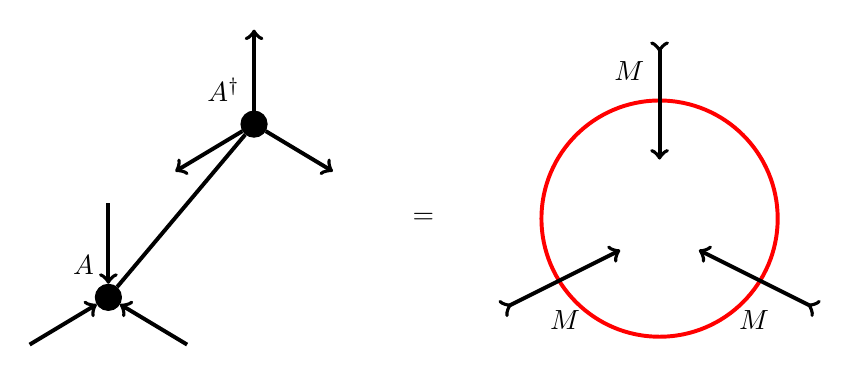
\begin{tikzpicture}
                \node[circle,draw=black,fill=black,minimum size=5pt,label={110:$A$}] (T) at (0,-1) {};
                \node[circle,draw=black,fill=black,minimum size=5pt,label={110:$A^\dag$}] (T2) at (1.85,1.2) {};
                \node (E) at (4,0) {$=$};
                \node[label={120:$M$}] (M1) at (7, 1.5) {};
                \node[label={-90:$M$}] (M2) at (8.2, -0.92) {};
                \node[label={-90:$M$}] (M3) at (5.8, -0.92) {};
                \draw[line width=0.5 mm] (T) -- (T2);
                \draw[<-, line width=0.5 mm] (T) -- +(0,1.2);
                \draw[<-, line width=0.5 mm] (T) -- (1, -1.6);
                \draw[<-, line width=0.5 mm] (T) -- (-1, -1.6);
                \draw[->, line width=0.5 mm] (T2) -- +(0,1.2);
                \draw[->, line width=0.5 mm] (T2) -- (2.85, 0.6);
                \draw[->, line width=0.5 mm] (T2) -- (0.85, 0.6);
                \draw[draw=red, line width=0.5 mm] (7, 0) circle (1.5);
                \draw[<-<, line width=0.5 mm] (7, 0.75) -- (7, 2.25);
                \draw[<-<, line width=0.5 mm] (7.5, -0.4) -- (9, -1.15);
                \draw[<-<, line width=0.5 mm] (6.5, -0.4) -- (5, -1.15);
            \end{tikzpicture}
            \caption{MPO-injective PEPS.}
            \label{tennet:fig:mpo_injectivity}
        \end{figure}
    }

    \begin{axiom}[Pulling-through]\index{pulling-through condition}
        One of the key features of topological order is that this cannot be detected locally, only a global measurement can show the existence of topologically ordered states. To this end we introduce an axiom such that one can pull an MPO through the lattice. Graphically this is shown in figure \ref{tennet:fig:pulling_through}.
        \begin{figure}[ht!]
            \centering
            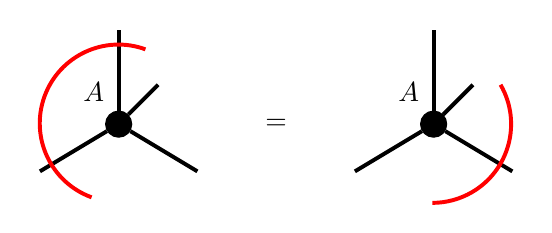
\begin{tikzpicture}
                \node[circle,draw=black,fill=black,minimum size=5pt,label={110:$A$}] (T) at (0,0) {};
                \node[circle,draw=black,fill=black,minimum size=5pt,label={110:$A$}] (T2) at (4,0) {};
                \node (E) at (2,0) {$=$};
                \draw[line width=0.5 mm] (T) -- +(0.5,0.5);
                \draw[line width=0.5 mm] (T) -- +(0,1.2);
                \draw[line width=0.5 mm] (T) -- (1, -0.6);
                \draw[line width=0.5 mm] (T) -- (-1, -0.6);
                \draw[line width=0.5 mm, draw=red] (0.34, 0.95) arc (70:250:1);
                \draw[line width=0.5 mm] (T2) -- +(0.5,0.5);
                \draw[line width=0.5 mm] (T2) -- +(0,1.2);
                \draw[line width=0.5 mm] (T2) -- (5, -0.6);
                \draw[line width=0.5 mm] (T2) -- (3, -0.6);
                \draw[line width=0.5 mm, draw=red] (4.85, 0.5) arc (30:-90:1);
            \end{tikzpicture}
            \caption{Pulling-through condition.}
            \label{tennet:fig:pulling_through}
        \end{figure}
    \end{axiom}

\subsection{MPO-symmetries for SPT phases}

    One can generalize the above framework to include not only pure topological order but also symmetry-protected topological order (see reference \cite{bultinck_mpo}). For this one has to slightly modify the axioms from the last section:
    \begin{axiom}[Pulling-through for SPT phases]\index{pulling-through condition}
        When pulling a symmetry-MPO through a tensor one has to act with a unitary on the physical level. Graphically this is shown in figure \ref{tennet:fig:pulling_through_spt}.
        \begin{figure}[ht!]
            \centering
            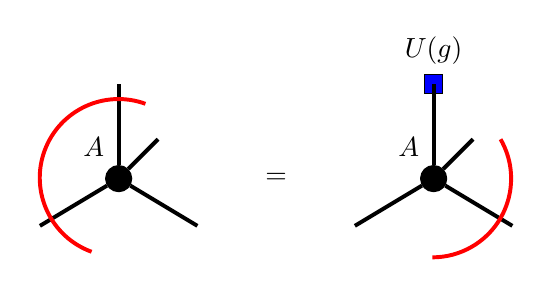
\begin{tikzpicture}
                \node[circle,draw=black,fill=black,minimum size=5pt,label={110:$A$}] (T) at (0,0) {};
                \node[circle,draw=black,fill=black,minimum size=5pt,label={110:$A$}] (T2) at (4,0) {};
                \node[rectangle, draw=black, fill=blue, minimum size=2pt, label={$U(g)$}] (U) at (4, 1.2) {};
                \node (E) at (2,0) {$=$};
                \draw[line width=0.5 mm] (T) -- +(0.5,0.5);
                \draw[line width=0.5 mm] (T) -- +(0,1.2);
                \draw[line width=0.5 mm] (T) -- (1, -0.6);
                \draw[line width=0.5 mm] (T) -- (-1, -0.6);
                \draw[line width=0.5 mm, draw=red] (0.34, 0.95) arc (70:250:1);
                \draw[line width=0.5 mm] (T2) -- +(0.5,0.5);
                \draw[line width=0.5 mm] (T2) -- +(0,1.2);
                \draw[line width=0.5 mm] (T2) -- (5, -0.6);
                \draw[line width=0.5 mm] (T2) -- (3, -0.6);
                \draw[line width=0.5 mm, draw=red] (4.85, 0.5) arc (30:-90:1);
            \end{tikzpicture}
            \caption{Pulling-through condition for SPT phases.}
            \label{tennet:fig:pulling_through_spt}
        \end{figure}
    \end{axiom}

\part{Appendices}
\begin{appendices}
\chapter{Derivations: Mathematics}

\section{Calculus}

\subsection{Proof of method \ref{calculus:borel_transform}}
	The function $F(x)$ is defined as follows:
	\begin{equation}
		F(x) = \ds\sum_{n=0}^{+\infty}\stylefrac{a_n}{n!}x^n
	\end{equation}
	We now perform a Borel transform:
	\begin{equation}
    		\begin{array}{ccl}
    			\ds\int_0^{+\infty}F(xt)e^{-t}dt&=&\ds\sum_{n=0}^N\int_0^{+\infty}\stylefrac{a_n}{n!}x^nt^ne^{-t}dt\\
        		&=&\ds\sum_{n=0}^N\frac{a_n}{n!}x^n\int_0^{+\infty}t^ne^{-t}dt\\
		        &=&\ds\sum_{n=0}^N\frac{a_n}{n!}x^n\Gamma(n+1)\\
		        &=&\ds\sum_{n=0}^Na_nx^n
	    	\end{array}
       	\end{equation}
       	where we used the definition of the Gamma function \ref{calculus:gamma_function} on line 3 and the relation between the factorial function and the Gamma function \ref{calculus:gamma_factorial_relation} on line 4.\qed

\section{Linear algebra}
\subsection{Explanation for property \ref{linalgebra:grassmannian_construction}}\label{proof:stabilizer}

	Pick a subspace $W\in \text{Gr}(k, V)$. The stabilizer of $W$ with respect to $GL(V)$ is the set \[H_W = \{g\in GL(V)| g\cdot W = W\}\]
	Due to the transitivity of the group action we have that
	\[\forall X, Y\in Gr(k, V): \exists h\in GL(V): h\cdot X = Y\]
	So for every $U\in \text{Gr}(k, V)$ we can choose a group element $g_U$ such that $g_U\cdot W = U$. For all elements in the coset $g_UH_W = \{g_Uh\in GL(V)|h\in H_W\}$ the following equality is satisfied:
	\[(g_Uh_W)\cdot W = g_U\cdot (h_WW) = g_U\cdot W = U\]
	This implies that the map $\Phi:GL(V)/H_W \rightarrow \text{Gr}(k, V)$ is surjective.
	
	Now we need to prove that $\Phi$ is also injective. We give a proof by contradiction. Choose two distinct cosets $pH_W$ and $qH_W$. Then there exist two subspaces $P, Q\in \text{Gr}(k, V)$ such that $p\cdot W = P$ and $q\cdot W = Q$. Now assume that $P = Q$. This means that
	\begin{align*}
		&p\cdot W = q\cdot W\\
		\iff&(q^{-1}p)\cdot W = W\\
		\iff&q^{-1}p\in H_W\\
		\iff&qH_W\mathrel{\reflectbox{$\in$}}q(q^{-1}p) = p
	\end{align*}
	This would imply that $pH_W = qH_W$ which is in contradiction to our assumption. It follows that $P\neq Q$ and that $\Phi$ is injective.\qed

\subsection{Proof for the equality of definitions \ref{tensor:exterior_algebra} and \ref{tensor:adef_exterior_algebra}}
	\begin{equation}
		(u+v)\otimes(u+v) - u\otimes u - v\otimes v = u\otimes v + v\otimes u
	\end{equation}
	The LHS is an element of the ideal $I$ generated by $\{v\otimes v|v\in V\}$. Using the ideal generated by elements such as in the RHS gives the usual definition of the exterior algebra based on the wedge product as defined in \ref{tensor:wedge_product} because it imposes the relation $u\wedge v = -v\wedge u$.
	
	We do however have to pay attention to one little detail. As mentioned in \ref{tensor:adef_exterior_algebra} the general definition uses the ideal $I$ to construct the quotient space. The other construction is only equivalent when working over a field with a characteristic different from 2. This follows from the fact that we have to divide by 2 when trying to obtain the ideal $I$ from the RHS by setting $u=v$.

\section{Vector fields \& differential forms}
\subsection{Explanation for example \ref{manifolds:ex:lie_derivative_function}}\index{Landau!little-o notation}

	In this derivation we use the Landau little-o notation $o(t)$, i.e.:
	\begin{equation}
		\lim_{t\rightarrow0}\frac{o(t)}{t} = 0
	\end{equation}
	Now assume that $X$  is a smooth vector field and $f$ is a smooth function. Because the Lie derivative is a local operation we can work in a local chart such that $\gamma$ is (again locally) equivalent to a curve\footnotemark\ $\beta_p:U\rightarrow\mathbb{R}^n$ and such that we can expand $\beta_p(t)$ around $p\in U$:
	\begin{align}
		\mathcal{L}_Xf(p) &= \lim_{t\rightarrow0}\left[\stylefrac{f(\beta_p(0) + t\beta_p'(0) + o(t)) - f(p)}{t}\right]\nonumber\\
		&= \lim_{t\rightarrow0}\left[\stylefrac{f(p + tX(p) + o(t)) - f(p)}{t}\right]\nonumber\\
		&= \lim_{t\rightarrow0}\left[\stylefrac{f(p) + tDf(p)\cdot X(p) + o(t) - f(p)}{t}\right]\nonumber\\
		&= \sum_k\pderiv{f}{x^k}(p)X_k(p) + \lim_{t\rightarrow0}\stylefrac{o(t)}{t}\nonumber\\
		&= \sum_k\pderiv{f}{x^k}(p)X_k(p)\label{manifolds:lie_derivative_calc}
	\end{align}
	where we used the defining condition \ref{manifolds:integral_curve} for integral curves on line 2. If we now rewrite this equation as an operator equality, we obtain:
	\begin{equation}
		\boxed{\mathcal{L}_X = \sum_kX_k\pderiv{}{x^k}}
	\end{equation}
	\footnotetext{The vector field $X(p) = (p, Y(p))$ where $Y$ is a smooth vector field on $\mathbb{R}^n$ can also be identified with $Y$ itself. This is implicitly done in the derivation by using the notation $X$ for both vector fields.}
		
\subsection{Explanation for formula \ref{manifolds:ex:lie_derivative_vector_fields}}

	For vector fields we cannot just take the difference at two different points because the tangent spaces generally do not coincide. We can solve this by using the flow \ref{manifolds:flow}:
	\begin{equation}
		\label{derivmath:lie_derivative_vector_fields}
		\mathcal{L}_XY = \lim_{t\rightarrow0}\stylefrac{(T\sigma_t)^{-1}[X(\gamma_p(t))] - X(p)}{t}
	\end{equation}
	where the $T\sigma_t$ is the differential \ref{manifolds:differential} of the flow which satisfies $(T\sigma)^{-1} = T\sigma_{-t}$. To see that this definition makes sense we have to show that $(T\sigma_t)^{-1}[X(\gamma_p(t))]\in T_pM$. This goes as follows:
	\begin{align*}
		(T\sigma_t)^{-1}[X(\gamma_p(t))](f) &= T\sigma_{-t}[X(\gamma_p(t))](f)\\
		&= X(\sigma_{-t}\circ\gamma_p(t))(f\circ\sigma_{-t})\\
		&= X(\sigma_{-t}\circ\sigma_t(p))(f\circ\sigma_{-t})\\
		&= X(p)(f\circ\sigma_{-t})\\
		&\in T_pM
	\end{align*}
	for all $f\in C^k(M, \mathbb{R})$. On line 3 we used the definition of the flow \ref{manifolds:flow}.
		
	We can also rewrite the second term in the numerator of \ref{derivmath:lie_derivative_vector_fields} using the flow:
	\[
		X(p) = X(\sigma_0(p)) = T\sigma_0(X)
	\]
	Using the definition of the pushforward of vector fields \ref{manifolds:pushforward} the Lie derivative can be rewritten as:
	\begin{align*}
		\mathcal{L}_XY &= \lim_{t\rightarrow0}\stylefrac{\sigma_{-t*}X(\gamma_p(t)) - \sigma_{0*}X(\gamma_p(0))}{t}\\
		&= \left.\deriv{}{t}(\sigma_{-t*}X)(\gamma_p(t))\right|_{t=0}
	\end{align*}
	Or finally by using the relation between pushforward and pullback \ref{manifolds:pullback_pushforward} this becomes:
	\begin{equation}
		\boxed{\mathcal{L}_XY = \left.\deriv{}{t}(\sigma_t^*X)(\gamma_p(t))\right|_{t=0}}
	\end{equation}
		 
\subsection{Explanation for remark \ref{forms:vector_calculus}}

Looking at formula \ref{forms:function_derivative} for the exterior derivative of a smooth function and remembering the definition of the gradient \ref{vectorcalculus:gradient} we see that these two definitions appear very similar. The major difference lies in the fact that $\nabla f$ is a vector in $\mathbb{R}^3$ and $df$ is a covector in $\mathbb{R}^{*3}$. However there exists an isomorphism between these spaces and so we can identify $\nabla f$ and $df$.
		
		Similar relations hold for the rotor \ref{vectorcalculus:rotor} and divergence \ref{vectorcalculus:divergence}, however here we have to use a different construction as we will be working with the spaces $\Lambda^1$ and $\Lambda^2$. However we can use the Hodge star \ref{tensor:hodge_star} to obtain the correct dimensions.
		
		Consider a vector $\vector{f} = (f_1, f_2, f_3)$ where $f_i$ is smooth. Using these functions $f_i$ we can construct a 1-form $\alpha = f_1dx_1 + f_2dx_2 + f_3dx_3$ and a 2-form $\omega = f_1dx_2\wedge dx_3 + f_2dx_3\wedge dx_1 + f_3 dx_1\wedge dx_2$. After applying the exterior derivative (in the corresponding spaces) we obtain:
		\begin{align}
			d\alpha &= \left(\pderiv{f_3}{x_2} - \pderiv{f_2}{x_3}\right)dx_2\wedge dx_3 + \left(\pderiv{f_1}{x_3} - \pderiv{f_3}{x_1}\right)dx_3\wedge dx_1 + \left(\pderiv{f_2}{x_1} - \pderiv{f_1}{x_2}\right)dx_1\wedge dx_2 \nonumber\\
			d\omega &= \left(\pderiv{f_1}{x_1} + \pderiv{f_2}{x_2} + \pderiv{f_3}{x_3}\right)dx_1\wedge dx_2\wedge dx_3 \nonumber
		\end{align}
		Using result \ref{tensor:hodge_star_vectorcalculus} and the isomorphism $\sim\ :\mathbb{R}^{3*}\rightarrow\mathbb{R}^3$ we can rewrite this as:
		\begin{empheq}[box=\fbox]{align}
			\sim df &= \nabla f \\
			\sim (\ast d\alpha) &= \nabla\times\vector{f} \\
			\ast d\omega &= \nabla\cdot\vector{f}
		\end{empheq}

\chapter{\texorpdfstring{$G$-Structures}{G-Structures}}
	In the following table we give an overview of the more common $G$-structures one can define on a smooth (simply-connected) manifolds $M^n$.
	\begin{center}
		\begin{tabularx}{\textwidth}{|l|c|X|}
			 \hline
			 	Geometric structure&Structure group&Remarks\\
			 \hline
			 	Orientation&SL$_n(\mathbb{R})$&GL$^+_n(\mathbb{R})$ is sufficient for orientability. The special linear group gives rise to a volume form.\\
			 	Riemannian metric&$O(n)$&\\&&\\
			 	Almost-symplectic structure*&Sp$_{2k}(\mathbb{R})$&Integrability (in the form of a closed form) gives a symplectic manifold.\\&&\\
			 	Almost-complex structure*&GL$_k(\mathbb{C})$&Integrability (in the form of Newlander-Nirenberg) gives a complex manifold.\\&&\\
			 	Almost-Hermitian structure*&U$(k)$&Integrability gives a K\"ahler manifold.\\&&\\
			 	Calabi-Yau*&SU$(k)$&\\&&\\
			 	Hyperk\"ahler**&Sp$(k)$&It follows that every hyperk\"ahler implies Calabi-Yau.\\&&\\
			 	Quaternionic-K\"ahler**\footnotemark&$(\text{Sp}(k)\times\text{Sp}(1))/\mathbb{Z}_2$&These manifolds are not strictly K\"ahler since the structure group is not a subgroup of U$(2k)$.\\
			 \hline
		\end{tabularx}
	\end{center}
	\footnotetext{This definition additionally requires that $k>1$.}
	Structures marked with $\ast$ require the real dimension $n=2k$ to be even. Structures marked with $\ast\ast$ require the real dimension $n=4k$ to be a multiple of 4.
	
	\begin{remark*}
		This table is strongly related to the classification of (irreducible simply-connected non-symmetric) Riemannian manifolds by \textit{Berger}.
	\end{remark*}
\chapter{Derivations: Mathematical Physics}
\section{d'Alembert's principle}\label{deriv:lagrange}\index{Lagrangian}

    In the following derivation we assume the mass to be constant.
    \begin{align}
        &\sum_k \left(\vector{F}_k - \dot{\vector{p}}_k\right)\dot{\vector{r}}_k = 0\nonumber\\
        \iff&\sum_k \left(\vector{F}_k - \dot{\vector{p}}_k\right)\cdot\left(\sum_l\pderiv{\vector{r}}{q_l}\dot{q_l}\right) = 0\nonumber\\
        \iff&\sum_l\left(\sum_k\vector{F}_k\cdot\pderiv{\vector{r}}{q_l} - \sum_km\ddot{\vector{r}}\cdot\pderiv{\vector{r}}{q_l}\right)\dot{q_l} = 0\nonumber\\
        \iff&\sum_l\left(Q_l - \sum_km\ddot{\vector{r}}\cdot\pderiv{\vector{r}}{q_l}\right)\dot{q_l} = 0\label{lagrange_deriv:deriv1}
    \end{align}
    \noindent Now we look at the following derivative:
    \begin{align}
        &\deriv{}{t}\left(\dot{\vector{r}}\cdot\pderiv{\vector{r}}{q_l}\right) = \ddot{\vector{r}}\cdot\pderiv{\vector{r}}{q_l} + \dot{\vector{r}}\cdot\deriv{}{t}\left(\pderiv{\vector{r}}{q_l}\right)\nonumber\\
        \iff&\ddot{\vector{r}}\cdot\pderiv{\vector{r}}{q_l} = \deriv{}{t}\left(\dot{\vector{r}}\cdot\pderiv{\vector{r}}{q_l}\right) - \dot{\vector{r}}\cdot\deriv{}{t}\left(\pderiv{\vector{r}}{q_l}\right)\nonumber\\
        \iff&\ddot{\vector{r}}\cdot\pderiv{\vector{r}}{q_l} = \deriv{}{t}\left(\dot{\vector{r}}\cdot{\color{red}\underbrace{\textcolor{black}{\pderiv{\vector{r}}{q_l}}}_A}\right) - \dot{\vector{r}}\cdot\left(\pderiv{\dot{\vector{r}}}{q_l}\right).\label{lagrange_deriv:deriv2}
    \end{align}
    To evaluate A we can take a look at another derivative:
    \begin{align}
        \pderiv{\dot{\vector{r}}}{\dot{q}_l} &= \pderiv{}{\dot{q}_l}\left(\sum_k\pderiv{r}{q_k}\dot{q}_k\right)\nonumber\\
        &=\sum_k\pderiv{r}{q_k}\delta_{kl}\nonumber\\
        &=\pderiv{\vector{r}}{q_l}\nonumber\\
        &=\textcolor{red}{A}.\nonumber
    \end{align}
    Substituting this in formula \ref{lagrange_deriv:deriv2} gives
    \begin{align}
        \ddot{\vector{r}}\cdot\pderiv{\vector{r}}{q_l} &= \deriv{}{t}\left(\dot{\vector{r}}\cdot\pderiv{\dot{\vector{r}}}{\dot{q}_l}\right) - \dot{\vector{r}}\cdot\left(\pderiv{\dot{\vector{r}}}{q_l}\right)\nonumber\\
        &=\deriv{}{t}\left(\stylefrac{1}{2}\pderiv{\dot{\vector{r}}^2}{\dot{q}_l}\right) - \stylefrac{1}{2}\pderiv{\dot{\vector{r}}^2}{q_l}.\label{lagrange_deriv:deriv3}
    \end{align}
    If we multiply this by the mass $m$ and sum over all particles we get
    \begin{align}
        \sum_km_k\ddot{\vector{r}}_k\cdot\pderiv{\vector{r}_k}{q_l}=\ &\deriv{}{t}\pderiv{}{\dot{q}_l}\left(\sum_k\stylefrac{1}{2}m\dot{\vector{r}}_k^2\right) - \pderiv{}{q_l}\left(\sum_k\stylefrac{1}{2}m\dot{\vector{r}}_k^2\right)\nonumber\\
        =\ &\deriv{}{t}\pderiv{T}{\dot{q}_l} - \pderiv{T}{q_l}\label{lagrange_deriv:deriv4}
    \end{align}
    where we have denoted the total kinetic energy in the last line by $T$. Plugging this result into formula \ref{lagrange_deriv:deriv1} gives us
    \begin{gather}
        \label{lagrange_deriv:deriv5}
        \sum_l\left(Q_l - \deriv{}{t}\pderiv{T}{\dot{q}_l} - \pderiv{T}{q_l}\right)\dot{q_l} = 0.
    \end{gather}
    As all the $q_l$ are independent the following relation should hold for all $l$:
    \begin{align}
        &Q_l - \deriv{}{t}\left(\pderiv{T}{\dot{q}_l}\right) - \pderiv{T}{q_l} = 0\nonumber\\
        \iff&\deriv{}{t}\left(\pderiv{T}{\dot{q}_l}\right) - \pderiv{T}{q_l} = Q_l.\label{lagrange_deriv:first_kind}
    \end{align}
    This last equation is known as a \textbf{Lagrange equation of the first kind}.

    If we have a system with only conservative forces acting on it, we can write the force on the $i^{th}$ particle as
    \begin{gather}
        \label{lagrange_deriv:deriv7}
        F_i = -\nabla_iV.
    \end{gather}
    With this in mind, let's take a look at the derivative of the potential $V$ with respect to the $l^{th}$ generalized coordinate:
    \begin{gather}
        \label{lagrange_deriv:deriv8}
        \begin{aligned}
            \pderiv{V}{q_l} &= \sum_i\left(\nabla_iV\right)\cdot\pderiv{\vector{r}_i}{q_l}\\
            &=-Q_l.
        \end{aligned}
    \end{gather}
    The derivative of $V$ with respect to any generalized velocity $\dot{q}_l$ is trivially zero. This combined with the previous formula and with formula \ref{lagrange_deriv:first_kind} gives
    \begin{align}
        &\deriv{}{t}\left(\pderiv{T}{\dot{q}_l}\right) - \pderiv{T}{q_l} = Q_l\nonumber\\
        \iff&\deriv{}{t}\left(\pderiv{T}{\dot{q}_l}\right) - \pderiv{T}{q_l} = -\pderiv{V}{q_l} + \pderiv{V}{\dot{q}_l}\nonumber\\
        \iff&\deriv{}{t}\left(\pderiv{T}{\dot{q}_l} - \pderiv{V}{\dot{q}_l}\right) - \pderiv{}{q_l}\left(T - V\right) = 0.\label{lagrange:deriv9}
    \end{align}
    If we introduce a new variable $L:=T-V$, called the \textbf{Lagrangian}, we get the \textbf{Lagrangian equation of the second kind}:
    \begin{gather}
        \label{lagrange_deriv:second_kind}
        \deriv{}{t}\left(\pderiv{L}{\dot{q}_l}\right) - \pderiv{L}{q_l} = 0.
    \end{gather}

\section{Hamilton's principle}

    In this part we start from the principle of least action. First we recall the definition of the \textbf{action}:
    \begin{gather}
        \label{lagrange_deriv:action_integral}
        I[y] := \int_{t_1}^{t_2}L\left(y(t), \dot{y}(t), t\right)dt
    \end{gather}
    Now we want to require that this action is minimal for the physically relevant path (Hamilton's principle). To do this we define a family of paths:
    \begin{gather}
        \label{lagrange_deriv:family_of_paths}
        y(t, \alpha) = y(t) + \alpha\eta(t)
    \end{gather}
    where $\eta(t)$ is an arbitrary function with the following boundary conditions:
    \begin{gather}
        \begin{cases}
        \eta(t_1) = 0&\\
        \eta(t_2) = 0.&
        \end{cases}
    \end{gather}
    If we define the action integral over this family of paths, the integral \ref{lagrange_deriv:action_integral} becomes a function of $\alpha$:
    \begin{gather}
        \label{lagrange_deriv:action_integral_over_family}
        I(\alpha) = \int_{t_1}^{t_2}L\left(y(t,\alpha), \dot{y}(t, \alpha), t\right)dt.
    \end{gather}
    Requiring that the action integral is stationary for $y(t)$ (and thus $\alpha = 0$) is equivalent to
    \begin{gather}
        \label{lagrange_deriv:stationary_condition}
        \left(\deriv{I}{\alpha}\right)_{\alpha=0} = 0.
    \end{gather}
    This condition combined with formula \ref{lagrange_deriv:action_integral_over_family} gives us
    \begin{gather}
        \label{lagrange_deriv:derivative_of_integral}
        \deriv{I}{\alpha} = \int_{t_1}^{t_2}\deriv{}{\alpha}L\left(y(t,\alpha), \dot{y}(t, \alpha), t\right)dt.
    \end{gather}
    As we evaluate this derivative at $\alpha = 0$ we can replace $y(t, \alpha)$ by $y(t)$ due to definition \ref{lagrange_deriv:family_of_paths}.
    \begin{align}
        \deriv{I}{\alpha}&=\int_{t_1}^{t_2}\left[\pderiv{L}{y}\pderiv{y}{\alpha} + \pderiv{L}{\dot{y}}\pderiv{\dot{y}}{\alpha}\right]dt\nonumber\\
        &=\int_{t_1}^{t_2}\left[\pderiv{L}{y}\eta(t) + \pderiv{L}{\dot{y}}\dot{\eta}(t)\right]dt.
    \end{align}
    If we substitute $\pderiv{L}{\dot{y}} := h(t)$ and apply integration by parts to the second term in this integral, we get
    \begin{align}
        \deriv{I}{\alpha}&=\int_{t_1}^{t_2}\left[\pderiv{L}{y}\eta(x) + h(t)\dot{\eta}(t)\right]dt\nonumber\\
        &=\int_{t_1}^{t_2}\left[\pderiv{L}{y}\eta(t) + h(t)\deriv{\eta}{t}\right]dt\nonumber\\
        &=\int_{t_1}^{t_2}\pderiv{L}{y}\eta(t)dt + \eta(t_2)h(t_2) - \eta(t_1)h(t_1) - \int_{t_1}^{t_2}\deriv{}{t}\left(\pderiv{L}{\dot{y}}\right)\eta(t)dt.
    \end{align}
    Due to the initial conditions \ref{lagrange_deriv:stationary_condition} for the function $\eta(t)$, the two terms in the middle vanish and we obtain
    \begin{gather}
        \label{lagrange_deriv:final_integral}
        \deriv{I}{\alpha}=\int_{t_1}^{t_2}\left[\pderiv{L}{y} - \deriv{}{t}\left(\pderiv{L}{\dot{y}}\right)\right]\eta(t)dt.
    \end{gather}
    Furthermore, since the function $\eta(t)$ was arbitrary, the only possible way that this derivative can become zero is when the integrand is identically zero:
    \begin{gather}
        \label{lagrange_deriv:second_kind_with_hamilton}
        \pderiv{L}{y} - \deriv{}{t}\left(\pderiv{L}{\dot{y}}\right) = 0.
    \end{gather}
    If we compare this result with formula \ref{lagrange_deriv:second_kind} we see that we can also obtain the \textbf{Lagrangian equations of the second kind} by starting from the principle of least action. (Where the variable $y$ represents the generalized coordinates $q_l$ and the variable $\dot{y}$ represents the generalized velocities $\dot{q}_l$)

    \begin{remark}
        Differential equations of the form
        \begin{gather}
            \label{lagrange_deriv:euler_lagrange_equation}
            \pderiv{f}{y}(y, \dot{y}, x) = \deriv{}{x}\left(\pderiv{f}{\dot{y}}(y, \dot{y}, x)\right)
        \end{gather}
        are known as \textbf{Euler-Lagrange equations}.
    \end{remark}

\section{Noether's theorem \ref{qft:noethers_theorem}}\label{proof:noether}

    The general transformation rule for the Lagrangian is
    \begin{gather}
        \label{noether_deriv:1}
        \mathcal{L}(x)\rightarrow\mathcal{L}(x) + \alpha\ \delta\mathcal{L}(x).
    \end{gather}
    To have a symmetry, i.e. to keep the action invariant, the deformation factor has to be a 4-divergence:
    \begin{gather}
        \label{noether_deriv:2}
        \mathcal{L}(x)\rightarrow\mathcal{L}(x) + \alpha\partial_\mu\mathcal{J}^\mu(x).
    \end{gather}

    To obtain formula \ref{qft:conserved_current} we vary the Lagrangian explicitly:
    \begin{align*}
        \delta\mathcal{L} &= \pderiv{\mathcal{L}}{\phi}\delta\phi + \pderiv{\mathcal{L}}{(\partial_\mu\phi)}\delta(\partial_\mu\phi)\\
        &= \pderiv{\mathcal{L}}{\phi}\delta\phi + \partial_\mu\left(\pderiv{\mathcal{L}}{(\partial_\mu\phi)}\delta\phi\right) - \partial_\mu\left(\pderiv{\mathcal{L}}{(\partial_\mu\phi)}\right)\delta\phi\\
        &= \partial_\mu\left(\pderiv{\mathcal{L}}{(\partial_\mu\phi)}\delta\phi\right) + \left[\pderiv{\mathcal{L}}{\phi} - \pderiv{\mathcal{L}}{(\partial_\mu\phi)}\right]\delta\phi.
    \end{align*}
    The second term vanishes due to the Euler-Lagrange equation \ref{lagrange_deriv:second_kind_with_hamilton}. Combining these formulas gives us
    \begin{gather}
        \partial_\mu\left(\pderiv{\mathcal{L}}{(\partial_\mu\phi)}\delta\phi\right) - \partial_\mu\mathcal{J}^\mu(x) = 0.
    \end{gather}
    From this equation we can conclude that the current
    \begin{gather}
        j^\mu(x) = \pderiv{\mathcal{L}}{(\partial_\mu\phi)}\delta\phi - \mathcal{J}^\mu(x)
    \end{gather}
    is conserved.


\chapter{Derivations: Optics and Material Physics}

\section{Law of Lambert-Beer \ref{optics:lambert_beer}}

    From formula \ref{optics:dielectric_function_non_magnetic} we now that the complex refractive index can be written as \[\widetilde{n} = n+ik\] where $k$ is called the \textbf{extinction coefficient}. From classic optics we also know that in a material the speed of light obeys the following relation: \[c = \widetilde{n}v.\] It readily follows that the wave number (sadly also denoted by the letter $k$) can be written as \[k = \stylefrac{\omega}{v} = \widetilde{n}\stylefrac{\omega}{c}.\] From classic electromagnetism we know that a plane wave can be written as \[E(x, t) = \text{Re}\big\{A\ \text{exp}\left[i(kx - \omega t + \phi)\right]\big\}.\] So after putting everything together we obtain \[E(x, t) = \text{Re}\left\{A\ \text{exp}\left[i\left((n+ik)\stylefrac{\omega}{c}x - \omega t + \phi\right)\right]\right\}.\] or also:\[E(x, t) = \text{Re}\left\{A\ \text{exp}\left(in\stylefrac{\omega}{c}x\right)\cdot\text{exp}\left(-k\stylefrac{\omega}{c}x\right)\cdot\text{exp}\left(-i\omega t\right)\cdot\text{exp}\left(i\phi\right)\right\}\] We also know that the intensity is given by the following relation:\[I(x) = |E(x)|^2 = E^*(x)\cdot E(x).\]
    This implies that only the second exponential factor will remain. Dividing the result by its value at $x=0$ gives \[\stylefrac{I(x)}{I(0)} = \stylefrac{E(x)\cdot E^*(x)}{E(0)\cdot E^*(0)} = \text{exp}\left(-\stylefrac{2k\omega}{c}x\right) = \text{exp}(-\alpha x)\]
    where $\alpha$ is the absorption coefficient as defined in formula \ref{optics:absorption_coefficient}.\qed

\section{Schottky defects \ref{maphy:schottky_defects}}\label{deriv:schottky_defects}\index{Schottky!defect}\index{Frenkel pair}

    Let $E_v$ be the energy needed to remove a particle from its lattice point and move it to the surface. We will neglect any surface effects and assume that the the energy $E_v$ is independent of the distance to the surface.

    The total energy of all vacancies is then given by $E = nE_v$. The number of possible microstates is
    \begin{gather}
        \Omega = \stylefrac{(N+n)!}{N!n!}
    \end{gather}
    where we used the fact that the removal of $n$ particles creates $n$ more lattice points at the surface. Using Boltzmann's entropy formula \ref{statmech:boltzmann_formula} and Stirling's formula we obtain
    \begin{gather}
        S(N, n) = k\ln\Omega = k\big[(N+n)\ln(N+n) -n\ln n - N\ln N \big].
    \end{gather}
    Using \ref{statmech:temperature} we can find the temperature
    \begin{gather}
        \stylefrac{1}{T} = \left(\pderiv{S}{E}\right)_{N, V} = \deriv{S}{n}\deriv{n}{E} = \frac{k}{E_v}\ln\frac{N+n}{n}
    \end{gather}
    which can be rewritten as
    \begin{gather}
        \stylefrac{n}{N + n} = \exp\left(-\frac{E_v}{kT}\right).
    \end{gather}
    The density of Frenkel pairs can be derived analogously.

\chapter{Derivations: Classical Mechanics}

\section{Moments of inertia}\label{deriv:inertia}\index{inertia}

    In this section we will use formula \ref{forces:moment_of_inertia} to calculate the moment of inertia.

\subsection{Disk}

    The volume of a (solid) disk is given by
    \begin{gather}
        V_{disk} = \pi R^2d
    \end{gather}
    where $R$ is the radius and $d$ is the thickness. The mass density is then given by
    \begin{gather}
        \rho = \frac{M}{\pi R^2d}.
    \end{gather}
    Using cylindrical coordinates the moment of inertia becomes
    \begin{align}
        I &= \frac{M}{\pi R^2d}\int_0^{2\pi}d\varphi\int_0^ddz\int_0^Rr^3dr\\
        &= \frac{M}{\pi R^2d}2\pi d\frac{R^4}{4}\\
        &= \frac{1}{2}MR^2.
    \end{align}

\subsection{Solid sphere}

    The volume of a solid sphere is given by
    \begin{gather}
        V_{sphere} = \frac{4}{3}\pi R^3
    \end{gather}
    where $R$ is the radius. The mass density is then given by
    \begin{gather}
        \rho = \frac{M}{\frac{4}{3}\pi R^3}.
    \end{gather}
    We will use spherical coordinates to derive the moment of inertia, but we have to be careful. The $r$ in formula \ref{forces:moment_of_inertia} is the distance between a point in the body and the axis of rotation. So it is not the same as the $r$ in spherical coordinates which is the distance between a point and the origin. However, the relation between these two quantities is easily found using basic geometry to be:
    \begin{gather}
        r = r'\sin\theta
    \end{gather}
    where $r'$ is the spherical coordinate. Now we can calculate the moment of inertia as follows:
    \begin{align}
        I &= \frac{M}{\frac{4}{3}\pi R^3} \int_0^{2\pi}d\varphi\int_0^Rr'^{^4}dr'\int_0^\pi\sin^3\theta d\theta\\
        &= \frac{M}{\frac{4}{3}\pi R^3} 2\pi \frac{R^5}{5} \frac{4}{3}\\
        &= \frac{2}{5}MR^2.
    \end{align}
\chapter{Units and symbols}

\begin{table}[h]
	\centering
	\begin{tabular}{|c|c|}
		\hline
		pk&745.7 W\\
		\hline
	\end{tabular}
	\caption{Units}
\end{table}
\end{appendices}

\nomenclature[O_zsymisisom]{$\cong$}{is isomorphic to}
\nomenclature[O_zsymisapprox]{$\approx$}{is approximately equal to}
\nomenclature[O_zsymmap]{$\mapsto$}{mapsto}
\nomenclature[O_zsymisincl]{$\hookrightarrow$}{is included in}
\nomenclature[O_zsymangle]{$\sphericalangle(v, w)$}{Angle between the vectors $v$ and $w$.}
\nomenclature[O_zsymbincart]{$X\times Y$}{Cartesian product of the sets $X$ and $Y$.}
\nomenclature[O_zsymids]{$\mathbbm{1}_X$}{Identity map on the set $X$.}
\nomenclature[O_e]{$e$}{Identity element of a group.}
\nomenclature[S_zsyminto]{$]a, b[$}{Open interval}
\nomenclature[S_zsymintc]{$[a, b]$}{Closed interval}
\nomenclature[S_zsymempty]{$\emptyset$}{Empty set}
\nomenclature[S_Sn]{$S^n$}{Standard $n$-sphere}
\nomenclature[S_Tn]{$T^n$}{Standard $n$-torus. Cartesian product of $n$ times $S^1$.}
\nomenclature[S_Dn]{$D^n$}{Standard $n$-disk}

%Print symbol list
\printnomenclature

\nocite{*}
\bibliographystyle{unsrt}
\bibliography{Biblio}

\printindex

\end{document}
